\documentclass[twoside]{book}

% Packages required by doxygen
\usepackage{fixltx2e}
\usepackage{calc}
\usepackage{doxygen}
\usepackage[export]{adjustbox} % also loads graphicx
\usepackage{graphicx}
\usepackage[utf8]{inputenc}
\usepackage{makeidx}
\usepackage{multicol}
\usepackage{multirow}
\PassOptionsToPackage{warn}{textcomp}
\usepackage{textcomp}
\usepackage[nointegrals]{wasysym}
\usepackage[table]{xcolor}

% Font selection
\usepackage[T1]{fontenc}
\usepackage[scaled=.90]{helvet}
\usepackage{courier}
\usepackage{amssymb}
\usepackage{sectsty}
\renewcommand{\familydefault}{\sfdefault}
\allsectionsfont{%
  \fontseries{bc}\selectfont%
  \color{darkgray}%
}
\renewcommand{\DoxyLabelFont}{%
  \fontseries{bc}\selectfont%
  \color{darkgray}%
}
\newcommand{\+}{\discretionary{\mbox{\scriptsize$\hookleftarrow$}}{}{}}

% Page & text layout
\usepackage{geometry}
\geometry{%
  a4paper,%
  top=2.5cm,%
  bottom=2.5cm,%
  left=2.5cm,%
  right=2.5cm%
}
\tolerance=750
\hfuzz=15pt
\hbadness=750
\setlength{\emergencystretch}{15pt}
\setlength{\parindent}{0cm}
\setlength{\parskip}{3ex plus 2ex minus 2ex}
\makeatletter
\renewcommand{\paragraph}{%
  \@startsection{paragraph}{4}{0ex}{-1.0ex}{1.0ex}{%
    \normalfont\normalsize\bfseries\SS@parafont%
  }%
}
\renewcommand{\subparagraph}{%
  \@startsection{subparagraph}{5}{0ex}{-1.0ex}{1.0ex}{%
    \normalfont\normalsize\bfseries\SS@subparafont%
  }%
}
\makeatother

% Headers & footers
\usepackage{fancyhdr}
\pagestyle{fancyplain}
\fancyhead[LE]{\fancyplain{}{\bfseries\thepage}}
\fancyhead[CE]{\fancyplain{}{}}
\fancyhead[RE]{\fancyplain{}{\bfseries\leftmark}}
\fancyhead[LO]{\fancyplain{}{\bfseries\rightmark}}
\fancyhead[CO]{\fancyplain{}{}}
\fancyhead[RO]{\fancyplain{}{\bfseries\thepage}}
\fancyfoot[LE]{\fancyplain{}{}}
\fancyfoot[CE]{\fancyplain{}{}}
\fancyfoot[RE]{\fancyplain{}{\bfseries\scriptsize Generated by Doxygen }}
\fancyfoot[LO]{\fancyplain{}{\bfseries\scriptsize Generated by Doxygen }}
\fancyfoot[CO]{\fancyplain{}{}}
\fancyfoot[RO]{\fancyplain{}{}}
\renewcommand{\footrulewidth}{0.4pt}
\renewcommand{\chaptermark}[1]{%
  \markboth{#1}{}%
}
\renewcommand{\sectionmark}[1]{%
  \markright{\thesection\ #1}%
}

% Indices & bibliography
\usepackage{natbib}
\usepackage[titles]{tocloft}
\setcounter{tocdepth}{3}
\setcounter{secnumdepth}{5}
\makeindex

% Hyperlinks (required, but should be loaded last)
\usepackage{ifpdf}
\ifpdf
  \usepackage[pdftex,pagebackref=true]{hyperref}
\else
  \usepackage[ps2pdf,pagebackref=true]{hyperref}
\fi
\hypersetup{%
  colorlinks=true,%
  linkcolor=blue,%
  citecolor=blue,%
  unicode%
}

% Custom commands
\newcommand{\clearemptydoublepage}{%
  \newpage{\pagestyle{empty}\cleardoublepage}%
}

\usepackage{caption}
\captionsetup{labelsep=space,justification=centering,font={bf},singlelinecheck=off,skip=4pt,position=top}

%===== C O N T E N T S =====

\begin{document}

% Titlepage & ToC
\hypersetup{pageanchor=false,
             bookmarksnumbered=true,
             pdfencoding=unicode
            }
\pagenumbering{roman}
\begin{titlepage}
\vspace*{7cm}
\begin{center}%
{\Large Virtual Zoo \\[1ex]\large V\+Z03 }\\
\vspace*{1cm}
{\large Generated by Doxygen 1.8.11}\\
\end{center}
\end{titlepage}
\clearemptydoublepage
\tableofcontents
\clearemptydoublepage
\pagenumbering{arabic}
\hypersetup{pageanchor=true}

%--- Begin generated contents ---
\chapter{virtual-\/zoo}
\label{md_README}
\hypertarget{md_README}{}
Tugas Besar 1 I\+F2210 O\+OP \+: Virtual \hyperlink{classZoo}{Zoo} (Cpp)

Cara menjalankan virtual zoo
\begin{DoxyEnumerate}
\item Ketik make di cmd untuk melakukan kompilasi
\item Ketik cd bin
\item Ketik ./main
\end{DoxyEnumerate}

Catatan\+: Input dapat dilakukan dengan mengubah konten dari zoo.\+txt, animal.\+txt, dan cage.\+txt 
\chapter{Hierarchical Index}
\section{Class Hierarchy}
This inheritance list is sorted roughly, but not completely, alphabetically\+:\begin{DoxyCompactList}
\item \contentsline{section}{Carnivore}{\pageref{classCarnivore}}{}
\begin{DoxyCompactList}
\item \contentsline{section}{Alligator}{\pageref{classAlligator}}{}
\item \contentsline{section}{Dolphin}{\pageref{classDolphin}}{}
\item \contentsline{section}{Eagle}{\pageref{classEagle}}{}
\item \contentsline{section}{Frog}{\pageref{classFrog}}{}
\item \contentsline{section}{Komodo}{\pageref{classKomodo}}{}
\item \contentsline{section}{Lion}{\pageref{classLion}}{}
\item \contentsline{section}{Piranha}{\pageref{classPiranha}}{}
\item \contentsline{section}{Tiger}{\pageref{classTiger}}{}
\item \contentsline{section}{Whale}{\pageref{classWhale}}{}
\end{DoxyCompactList}
\item \contentsline{section}{Driver}{\pageref{classDriver}}{}
\item \contentsline{section}{Herbivore}{\pageref{classHerbivore}}{}
\begin{DoxyCompactList}
\item \contentsline{section}{Bear}{\pageref{classBear}}{}
\item \contentsline{section}{Chimpanzee}{\pageref{classChimpanzee}}{}
\item \contentsline{section}{Elephant}{\pageref{classElephant}}{}
\item \contentsline{section}{Giraffe}{\pageref{classGiraffe}}{}
\item \contentsline{section}{Hippopotamus}{\pageref{classHippopotamus}}{}
\item \contentsline{section}{Orangutan}{\pageref{classOrangutan}}{}
\end{DoxyCompactList}
\item \contentsline{section}{Omnivore}{\pageref{classOmnivore}}{}
\begin{DoxyCompactList}
\item \contentsline{section}{Bat}{\pageref{classBat}}{}
\item \contentsline{section}{Blue\+Tang}{\pageref{classBlueTang}}{}
\item \contentsline{section}{Cendrawasih}{\pageref{classCendrawasih}}{}
\item \contentsline{section}{Clownfish}{\pageref{classClownfish}}{}
\item \contentsline{section}{Cockatoo}{\pageref{classCockatoo}}{}
\item \contentsline{section}{Macau}{\pageref{classMacau}}{}
\item \contentsline{section}{Owl}{\pageref{classOwl}}{}
\item \contentsline{section}{Puff\+Fish}{\pageref{classPuffFish}}{}
\item \contentsline{section}{Turtle}{\pageref{classTurtle}}{}
\end{DoxyCompactList}
\item \contentsline{section}{Zoo\+:\+:Proxy}{\pageref{classZoo_1_1Proxy}}{}
\item \contentsline{section}{Renderable}{\pageref{classRenderable}}{}
\begin{DoxyCompactList}
\item \contentsline{section}{Animal}{\pageref{classAnimal}}{}
\begin{DoxyCompactList}
\item \contentsline{section}{Flying\+Animal}{\pageref{classFlyingAnimal}}{}
\begin{DoxyCompactList}
\item \contentsline{section}{Bat}{\pageref{classBat}}{}
\item \contentsline{section}{Cendrawasih}{\pageref{classCendrawasih}}{}
\item \contentsline{section}{Cockatoo}{\pageref{classCockatoo}}{}
\item \contentsline{section}{Eagle}{\pageref{classEagle}}{}
\item \contentsline{section}{Macau}{\pageref{classMacau}}{}
\item \contentsline{section}{Owl}{\pageref{classOwl}}{}
\end{DoxyCompactList}
\item \contentsline{section}{Land\+Animal}{\pageref{classLandAnimal}}{}
\begin{DoxyCompactList}
\item \contentsline{section}{Alligator}{\pageref{classAlligator}}{}
\item \contentsline{section}{Bear}{\pageref{classBear}}{}
\item \contentsline{section}{Chimpanzee}{\pageref{classChimpanzee}}{}
\item \contentsline{section}{Elephant}{\pageref{classElephant}}{}
\item \contentsline{section}{Frog}{\pageref{classFrog}}{}
\item \contentsline{section}{Giraffe}{\pageref{classGiraffe}}{}
\item \contentsline{section}{Hippopotamus}{\pageref{classHippopotamus}}{}
\item \contentsline{section}{Komodo}{\pageref{classKomodo}}{}
\item \contentsline{section}{Lion}{\pageref{classLion}}{}
\item \contentsline{section}{Orangutan}{\pageref{classOrangutan}}{}
\item \contentsline{section}{Tiger}{\pageref{classTiger}}{}
\item \contentsline{section}{Turtle}{\pageref{classTurtle}}{}
\end{DoxyCompactList}
\item \contentsline{section}{Water\+Animal}{\pageref{classWaterAnimal}}{}
\begin{DoxyCompactList}
\item \contentsline{section}{Alligator}{\pageref{classAlligator}}{}
\item \contentsline{section}{Blue\+Tang}{\pageref{classBlueTang}}{}
\item \contentsline{section}{Clownfish}{\pageref{classClownfish}}{}
\item \contentsline{section}{Dolphin}{\pageref{classDolphin}}{}
\item \contentsline{section}{Frog}{\pageref{classFrog}}{}
\item \contentsline{section}{Hippopotamus}{\pageref{classHippopotamus}}{}
\item \contentsline{section}{Piranha}{\pageref{classPiranha}}{}
\item \contentsline{section}{Puff\+Fish}{\pageref{classPuffFish}}{}
\item \contentsline{section}{Turtle}{\pageref{classTurtle}}{}
\item \contentsline{section}{Whale}{\pageref{classWhale}}{}
\end{DoxyCompactList}
\end{DoxyCompactList}
\item \contentsline{section}{Cage}{\pageref{classCage}}{}
\item \contentsline{section}{Cell}{\pageref{classCell}}{}
\begin{DoxyCompactList}
\item \contentsline{section}{Facility}{\pageref{classFacility}}{}
\begin{DoxyCompactList}
\item \contentsline{section}{Park}{\pageref{classPark}}{}
\item \contentsline{section}{Restaurant}{\pageref{classRestaurant}}{}
\item \contentsline{section}{Road}{\pageref{classRoad}}{}
\begin{DoxyCompactList}
\item \contentsline{section}{Entrance}{\pageref{classEntrance}}{}
\item \contentsline{section}{Exit}{\pageref{classExit}}{}
\end{DoxyCompactList}
\end{DoxyCompactList}
\item \contentsline{section}{Habitat}{\pageref{classHabitat}}{}
\begin{DoxyCompactList}
\item \contentsline{section}{Air\+Habitat}{\pageref{classAirHabitat}}{}
\item \contentsline{section}{Land\+Habitat}{\pageref{classLandHabitat}}{}
\item \contentsline{section}{Water\+Habitat}{\pageref{classWaterHabitat}}{}
\end{DoxyCompactList}
\end{DoxyCompactList}
\end{DoxyCompactList}
\item \contentsline{section}{Vertebrate}{\pageref{classVertebrate}}{}
\begin{DoxyCompactList}
\item \contentsline{section}{Amphibia}{\pageref{classAmphibia}}{}
\begin{DoxyCompactList}
\item \contentsline{section}{Frog}{\pageref{classFrog}}{}
\end{DoxyCompactList}
\item \contentsline{section}{Aves}{\pageref{classAves}}{}
\begin{DoxyCompactList}
\item \contentsline{section}{Bat}{\pageref{classBat}}{}
\item \contentsline{section}{Cendrawasih}{\pageref{classCendrawasih}}{}
\item \contentsline{section}{Cockatoo}{\pageref{classCockatoo}}{}
\item \contentsline{section}{Eagle}{\pageref{classEagle}}{}
\item \contentsline{section}{Macau}{\pageref{classMacau}}{}
\item \contentsline{section}{Owl}{\pageref{classOwl}}{}
\end{DoxyCompactList}
\item \contentsline{section}{Mammalia}{\pageref{classMammalia}}{}
\begin{DoxyCompactList}
\item \contentsline{section}{Bear}{\pageref{classBear}}{}
\item \contentsline{section}{Chimpanzee}{\pageref{classChimpanzee}}{}
\item \contentsline{section}{Dolphin}{\pageref{classDolphin}}{}
\item \contentsline{section}{Elephant}{\pageref{classElephant}}{}
\item \contentsline{section}{Giraffe}{\pageref{classGiraffe}}{}
\item \contentsline{section}{Hippopotamus}{\pageref{classHippopotamus}}{}
\item \contentsline{section}{Lion}{\pageref{classLion}}{}
\item \contentsline{section}{Orangutan}{\pageref{classOrangutan}}{}
\item \contentsline{section}{Tiger}{\pageref{classTiger}}{}
\item \contentsline{section}{Whale}{\pageref{classWhale}}{}
\end{DoxyCompactList}
\item \contentsline{section}{Pisces}{\pageref{classPisces}}{}
\begin{DoxyCompactList}
\item \contentsline{section}{Blue\+Tang}{\pageref{classBlueTang}}{}
\item \contentsline{section}{Clownfish}{\pageref{classClownfish}}{}
\item \contentsline{section}{Piranha}{\pageref{classPiranha}}{}
\item \contentsline{section}{Puff\+Fish}{\pageref{classPuffFish}}{}
\end{DoxyCompactList}
\item \contentsline{section}{Reptilia}{\pageref{classReptilia}}{}
\begin{DoxyCompactList}
\item \contentsline{section}{Alligator}{\pageref{classAlligator}}{}
\item \contentsline{section}{Komodo}{\pageref{classKomodo}}{}
\item \contentsline{section}{Turtle}{\pageref{classTurtle}}{}
\end{DoxyCompactList}
\end{DoxyCompactList}
\item \contentsline{section}{Zoo}{\pageref{classZoo}}{}
\end{DoxyCompactList}

\chapter{Class Index}
\section{Class List}
Here are the classes, structs, unions and interfaces with brief descriptions\+:\begin{DoxyCompactList}
\item\contentsline{section}{\hyperlink{classAirHabitat}{Air\+Habitat} }{\pageref{classAirHabitat}}{}
\item\contentsline{section}{\hyperlink{classAlligator}{Alligator} }{\pageref{classAlligator}}{}
\item\contentsline{section}{\hyperlink{classAmphibia}{Amphibia} }{\pageref{classAmphibia}}{}
\item\contentsline{section}{\hyperlink{classAnimal}{Animal} }{\pageref{classAnimal}}{}
\item\contentsline{section}{\hyperlink{classAves}{Aves} }{\pageref{classAves}}{}
\item\contentsline{section}{\hyperlink{classBat}{Bat} }{\pageref{classBat}}{}
\item\contentsline{section}{\hyperlink{classBear}{Bear} }{\pageref{classBear}}{}
\item\contentsline{section}{\hyperlink{classBlueTang}{Blue\+Tang} }{\pageref{classBlueTang}}{}
\item\contentsline{section}{\hyperlink{classCage}{Cage} }{\pageref{classCage}}{}
\item\contentsline{section}{\hyperlink{classCarnivore}{Carnivore} }{\pageref{classCarnivore}}{}
\item\contentsline{section}{\hyperlink{classCell}{Cell} }{\pageref{classCell}}{}
\item\contentsline{section}{\hyperlink{classCendrawasih}{Cendrawasih} }{\pageref{classCendrawasih}}{}
\item\contentsline{section}{\hyperlink{classChimpanzee}{Chimpanzee} }{\pageref{classChimpanzee}}{}
\item\contentsline{section}{\hyperlink{classClownfish}{Clownfish} }{\pageref{classClownfish}}{}
\item\contentsline{section}{\hyperlink{classCockatoo}{Cockatoo} }{\pageref{classCockatoo}}{}
\item\contentsline{section}{\hyperlink{classDolphin}{Dolphin} }{\pageref{classDolphin}}{}
\item\contentsline{section}{\hyperlink{classDriver}{Driver} }{\pageref{classDriver}}{}
\item\contentsline{section}{\hyperlink{classEagle}{Eagle} }{\pageref{classEagle}}{}
\item\contentsline{section}{\hyperlink{classElephant}{Elephant} }{\pageref{classElephant}}{}
\item\contentsline{section}{\hyperlink{classEntrance}{Entrance} }{\pageref{classEntrance}}{}
\item\contentsline{section}{\hyperlink{classExit}{Exit} }{\pageref{classExit}}{}
\item\contentsline{section}{\hyperlink{classFacility}{Facility} }{\pageref{classFacility}}{}
\item\contentsline{section}{\hyperlink{classFlyingAnimal}{Flying\+Animal} }{\pageref{classFlyingAnimal}}{}
\item\contentsline{section}{\hyperlink{classFrog}{Frog} }{\pageref{classFrog}}{}
\item\contentsline{section}{\hyperlink{classGiraffe}{Giraffe} }{\pageref{classGiraffe}}{}
\item\contentsline{section}{\hyperlink{classHabitat}{Habitat} }{\pageref{classHabitat}}{}
\item\contentsline{section}{\hyperlink{classHerbivore}{Herbivore} }{\pageref{classHerbivore}}{}
\item\contentsline{section}{\hyperlink{classHippopotamus}{Hippopotamus} }{\pageref{classHippopotamus}}{}
\item\contentsline{section}{\hyperlink{classKomodo}{Komodo} }{\pageref{classKomodo}}{}
\item\contentsline{section}{\hyperlink{classLandAnimal}{Land\+Animal} }{\pageref{classLandAnimal}}{}
\item\contentsline{section}{\hyperlink{classLandHabitat}{Land\+Habitat} }{\pageref{classLandHabitat}}{}
\item\contentsline{section}{\hyperlink{classLion}{Lion} }{\pageref{classLion}}{}
\item\contentsline{section}{\hyperlink{classMacau}{Macau} }{\pageref{classMacau}}{}
\item\contentsline{section}{\hyperlink{classMammalia}{Mammalia} }{\pageref{classMammalia}}{}
\item\contentsline{section}{\hyperlink{classOmnivore}{Omnivore} }{\pageref{classOmnivore}}{}
\item\contentsline{section}{\hyperlink{classOrangutan}{Orangutan} }{\pageref{classOrangutan}}{}
\item\contentsline{section}{\hyperlink{classOwl}{Owl} }{\pageref{classOwl}}{}
\item\contentsline{section}{\hyperlink{classPark}{Park} }{\pageref{classPark}}{}
\item\contentsline{section}{\hyperlink{classPiranha}{Piranha} }{\pageref{classPiranha}}{}
\item\contentsline{section}{\hyperlink{classPisces}{Pisces} }{\pageref{classPisces}}{}
\item\contentsline{section}{\hyperlink{classZoo_1_1Proxy}{Zoo\+::\+Proxy} }{\pageref{classZoo_1_1Proxy}}{}
\item\contentsline{section}{\hyperlink{classPuffFish}{Puff\+Fish} }{\pageref{classPuffFish}}{}
\item\contentsline{section}{\hyperlink{classRenderable}{Renderable} }{\pageref{classRenderable}}{}
\item\contentsline{section}{\hyperlink{classReptilia}{Reptilia} }{\pageref{classReptilia}}{}
\item\contentsline{section}{\hyperlink{classRestaurant}{Restaurant} }{\pageref{classRestaurant}}{}
\item\contentsline{section}{\hyperlink{classRoad}{Road} }{\pageref{classRoad}}{}
\item\contentsline{section}{\hyperlink{classTiger}{Tiger} }{\pageref{classTiger}}{}
\item\contentsline{section}{\hyperlink{classTurtle}{Turtle} }{\pageref{classTurtle}}{}
\item\contentsline{section}{\hyperlink{classVertebrate}{Vertebrate} }{\pageref{classVertebrate}}{}
\item\contentsline{section}{\hyperlink{classWaterAnimal}{Water\+Animal} }{\pageref{classWaterAnimal}}{}
\item\contentsline{section}{\hyperlink{classWaterHabitat}{Water\+Habitat} }{\pageref{classWaterHabitat}}{}
\item\contentsline{section}{\hyperlink{classWhale}{Whale} }{\pageref{classWhale}}{}
\item\contentsline{section}{\hyperlink{classZoo}{Zoo} }{\pageref{classZoo}}{}
\end{DoxyCompactList}

\chapter{File Index}
\section{File List}
Here is a list of all files with brief descriptions\+:\begin{DoxyCompactList}
\item\contentsline{section}{src/\hyperlink{main_8cpp}{main.\+cpp} }{\pageref{main_8cpp}}{}
\item\contentsline{section}{src/driver/\hyperlink{driver_8cpp}{driver.\+cpp} }{\pageref{driver_8cpp}}{}
\item\contentsline{section}{src/driver/\hyperlink{driver_8h}{driver.\+h} }{\pageref{driver_8h}}{}
\item\contentsline{section}{src/other/\hyperlink{color_8cpp}{color.\+cpp} }{\pageref{color_8cpp}}{}
\item\contentsline{section}{src/other/\hyperlink{color_8h}{color.\+h} }{\pageref{color_8h}}{}
\item\contentsline{section}{src/other/\hyperlink{sex_8h}{sex.\+h} }{\pageref{sex_8h}}{}
\item\contentsline{section}{src/renders/\hyperlink{cell_8cpp}{cell.\+cpp} }{\pageref{cell_8cpp}}{}
\item\contentsline{section}{src/renders/\hyperlink{cell_8h}{cell.\+h} }{\pageref{cell_8h}}{}
\item\contentsline{section}{src/renders/\hyperlink{renderable_8cpp}{renderable.\+cpp} }{\pageref{renderable_8cpp}}{}
\item\contentsline{section}{src/renders/\hyperlink{renderable_8h}{renderable.\+h} }{\pageref{renderable_8h}}{}
\item\contentsline{section}{src/renders/\hyperlink{renders_8h}{renders.\+h} }{\pageref{renders_8h}}{}
\item\contentsline{section}{src/renders/animals/\hyperlink{animal_8cpp}{animal.\+cpp} }{\pageref{animal_8cpp}}{}
\item\contentsline{section}{src/renders/animals/\hyperlink{animal_8h}{animal.\+h} }{\pageref{animal_8h}}{}
\item\contentsline{section}{src/renders/animals/\hyperlink{animals_8h}{animals.\+h} }{\pageref{animals_8h}}{}
\item\contentsline{section}{src/renders/animals/\hyperlink{flying__animal_8cpp}{flying\+\_\+animal.\+cpp} }{\pageref{flying__animal_8cpp}}{}
\item\contentsline{section}{src/renders/animals/\hyperlink{flying__animal_8h}{flying\+\_\+animal.\+h} }{\pageref{flying__animal_8h}}{}
\item\contentsline{section}{src/renders/animals/\hyperlink{land__animal_8cpp}{land\+\_\+animal.\+cpp} }{\pageref{land__animal_8cpp}}{}
\item\contentsline{section}{src/renders/animals/\hyperlink{land__animal_8h}{land\+\_\+animal.\+h} }{\pageref{land__animal_8h}}{}
\item\contentsline{section}{src/renders/animals/\hyperlink{species_8cpp}{species.\+cpp} }{\pageref{species_8cpp}}{}
\item\contentsline{section}{src/renders/animals/\hyperlink{species_8h}{species.\+h} }{\pageref{species_8h}}{}
\item\contentsline{section}{src/renders/animals/\hyperlink{water__animal_8cpp}{water\+\_\+animal.\+cpp} }{\pageref{water__animal_8cpp}}{}
\item\contentsline{section}{src/renders/animals/\hyperlink{water__animal_8h}{water\+\_\+animal.\+h} }{\pageref{water__animal_8h}}{}
\item\contentsline{section}{src/renders/animals/diet/\hyperlink{carnivore_8cpp}{carnivore.\+cpp} }{\pageref{carnivore_8cpp}}{}
\item\contentsline{section}{src/renders/animals/diet/\hyperlink{carnivore_8h}{carnivore.\+h} }{\pageref{carnivore_8h}}{}
\item\contentsline{section}{src/renders/animals/diet/\hyperlink{diet_8h}{diet.\+h} }{\pageref{diet_8h}}{}
\item\contentsline{section}{src/renders/animals/diet/\hyperlink{herbivore_8cpp}{herbivore.\+cpp} }{\pageref{herbivore_8cpp}}{}
\item\contentsline{section}{src/renders/animals/diet/\hyperlink{herbivore_8h}{herbivore.\+h} }{\pageref{herbivore_8h}}{}
\item\contentsline{section}{src/renders/animals/diet/\hyperlink{omnivore_8cpp}{omnivore.\+cpp} }{\pageref{omnivore_8cpp}}{}
\item\contentsline{section}{src/renders/animals/diet/\hyperlink{omnivore_8h}{omnivore.\+h} }{\pageref{omnivore_8h}}{}
\item\contentsline{section}{src/renders/animals/taxonomy/\hyperlink{amphibia_8cpp}{amphibia.\+cpp} }{\pageref{amphibia_8cpp}}{}
\item\contentsline{section}{src/renders/animals/taxonomy/\hyperlink{amphibia_8h}{amphibia.\+h} }{\pageref{amphibia_8h}}{}
\item\contentsline{section}{src/renders/animals/taxonomy/\hyperlink{aves_8cpp}{aves.\+cpp} }{\pageref{aves_8cpp}}{}
\item\contentsline{section}{src/renders/animals/taxonomy/\hyperlink{aves_8h}{aves.\+h} }{\pageref{aves_8h}}{}
\item\contentsline{section}{src/renders/animals/taxonomy/\hyperlink{mammalia_8cpp}{mammalia.\+cpp} }{\pageref{mammalia_8cpp}}{}
\item\contentsline{section}{src/renders/animals/taxonomy/\hyperlink{mammalia_8h}{mammalia.\+h} }{\pageref{mammalia_8h}}{}
\item\contentsline{section}{src/renders/animals/taxonomy/\hyperlink{pisces_8cpp}{pisces.\+cpp} }{\pageref{pisces_8cpp}}{}
\item\contentsline{section}{src/renders/animals/taxonomy/\hyperlink{pisces_8h}{pisces.\+h} }{\pageref{pisces_8h}}{}
\item\contentsline{section}{src/renders/animals/taxonomy/\hyperlink{reptilia_8cpp}{reptilia.\+cpp} }{\pageref{reptilia_8cpp}}{}
\item\contentsline{section}{src/renders/animals/taxonomy/\hyperlink{reptilia_8h}{reptilia.\+h} }{\pageref{reptilia_8h}}{}
\item\contentsline{section}{src/renders/animals/taxonomy/\hyperlink{taxonomy_8h}{taxonomy.\+h} }{\pageref{taxonomy_8h}}{}
\item\contentsline{section}{src/renders/animals/taxonomy/\hyperlink{vertebrate_8cpp}{vertebrate.\+cpp} }{\pageref{vertebrate_8cpp}}{}
\item\contentsline{section}{src/renders/animals/taxonomy/\hyperlink{vertebrate_8h}{vertebrate.\+h} }{\pageref{vertebrate_8h}}{}
\item\contentsline{section}{src/renders/cage/\hyperlink{cage_8cpp}{cage.\+cpp} }{\pageref{cage_8cpp}}{}
\item\contentsline{section}{src/renders/cage/\hyperlink{cage_8h}{cage.\+h} }{\pageref{cage_8h}}{}
\item\contentsline{section}{src/renders/facilities/\hyperlink{facilities_8h}{facilities.\+h} }{\pageref{facilities_8h}}{}
\item\contentsline{section}{src/renders/facilities/\hyperlink{facility_8cpp}{facility.\+cpp} }{\pageref{facility_8cpp}}{}
\item\contentsline{section}{src/renders/facilities/\hyperlink{facility_8h}{facility.\+h} }{\pageref{facility_8h}}{}
\item\contentsline{section}{src/renders/facilities/park/\hyperlink{park_8cpp}{park.\+cpp} }{\pageref{park_8cpp}}{}
\item\contentsline{section}{src/renders/facilities/park/\hyperlink{park_8h}{park.\+h} }{\pageref{park_8h}}{}
\item\contentsline{section}{src/renders/facilities/restaurant/\hyperlink{restaurant_8cpp}{restaurant.\+cpp} }{\pageref{restaurant_8cpp}}{}
\item\contentsline{section}{src/renders/facilities/restaurant/\hyperlink{restaurant_8h}{restaurant.\+h} }{\pageref{restaurant_8h}}{}
\item\contentsline{section}{src/renders/facilities/road/\hyperlink{road_8cpp}{road.\+cpp} }{\pageref{road_8cpp}}{}
\item\contentsline{section}{src/renders/facilities/road/\hyperlink{road_8h}{road.\+h} }{\pageref{road_8h}}{}
\item\contentsline{section}{src/renders/facilities/road/entrance/\hyperlink{entrance_8cpp}{entrance.\+cpp} }{\pageref{entrance_8cpp}}{}
\item\contentsline{section}{src/renders/facilities/road/entrance/\hyperlink{entrance_8h}{entrance.\+h} }{\pageref{entrance_8h}}{}
\item\contentsline{section}{src/renders/facilities/road/exit/\hyperlink{exit_8cpp}{exit.\+cpp} }{\pageref{exit_8cpp}}{}
\item\contentsline{section}{src/renders/facilities/road/exit/\hyperlink{exit_8h}{exit.\+h} }{\pageref{exit_8h}}{}
\item\contentsline{section}{src/renders/habitats/\hyperlink{air__habitat_8cpp}{air\+\_\+habitat.\+cpp} }{\pageref{air__habitat_8cpp}}{}
\item\contentsline{section}{src/renders/habitats/\hyperlink{air__habitat_8h}{air\+\_\+habitat.\+h} }{\pageref{air__habitat_8h}}{}
\item\contentsline{section}{src/renders/habitats/\hyperlink{habitat_8cpp}{habitat.\+cpp} }{\pageref{habitat_8cpp}}{}
\item\contentsline{section}{src/renders/habitats/\hyperlink{habitat_8h}{habitat.\+h} }{\pageref{habitat_8h}}{}
\item\contentsline{section}{src/renders/habitats/\hyperlink{habitats_8h}{habitats.\+h} }{\pageref{habitats_8h}}{}
\item\contentsline{section}{src/renders/habitats/\hyperlink{land__habitat_8cpp}{land\+\_\+habitat.\+cpp} }{\pageref{land__habitat_8cpp}}{}
\item\contentsline{section}{src/renders/habitats/\hyperlink{land__habitat_8h}{land\+\_\+habitat.\+h} }{\pageref{land__habitat_8h}}{}
\item\contentsline{section}{src/renders/habitats/\hyperlink{water__habitat_8cpp}{water\+\_\+habitat.\+cpp} }{\pageref{water__habitat_8cpp}}{}
\item\contentsline{section}{src/renders/habitats/\hyperlink{water__habitat_8h}{water\+\_\+habitat.\+h} }{\pageref{water__habitat_8h}}{}
\item\contentsline{section}{src/zoo/\hyperlink{Zoo_8cpp}{Zoo.\+cpp} }{\pageref{Zoo_8cpp}}{}
\item\contentsline{section}{src/zoo/\hyperlink{zoo_8h}{zoo.\+h} }{\pageref{zoo_8h}}{}
\item\contentsline{section}{src/zoo/\hyperlink{zoo__driver_8cpp}{zoo\+\_\+driver.\+cpp} }{\pageref{zoo__driver_8cpp}}{}
\end{DoxyCompactList}

\chapter{Class Documentation}
\hypertarget{classAirHabitat}{}\section{Air\+Habitat Class Reference}
\label{classAirHabitat}\index{Air\+Habitat@{Air\+Habitat}}


{\ttfamily \#include $<$air\+\_\+habitat.\+h$>$}



Inheritance diagram for Air\+Habitat\+:
\nopagebreak
\begin{figure}[H]
\begin{center}
\leavevmode
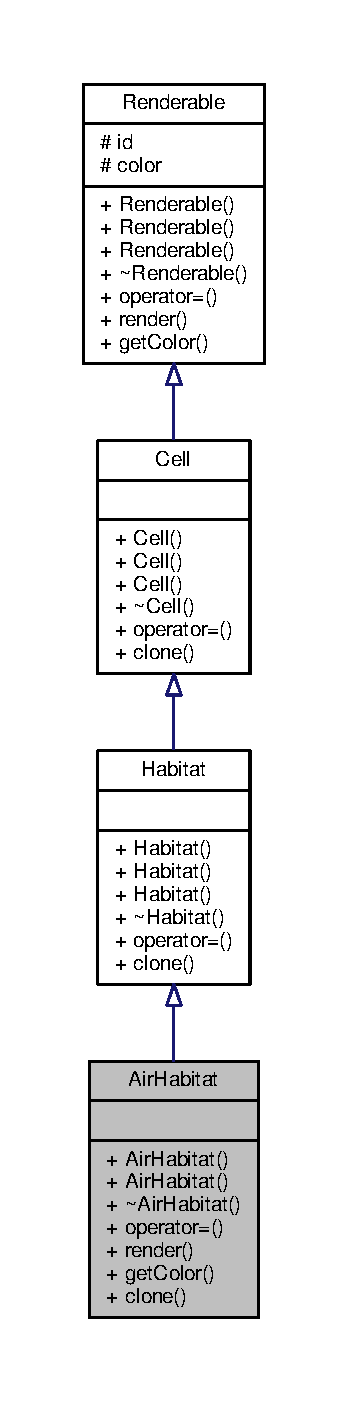
\includegraphics[height=550pt]{classAirHabitat__inherit__graph}
\end{center}
\end{figure}


Collaboration diagram for Air\+Habitat\+:
\nopagebreak
\begin{figure}[H]
\begin{center}
\leavevmode
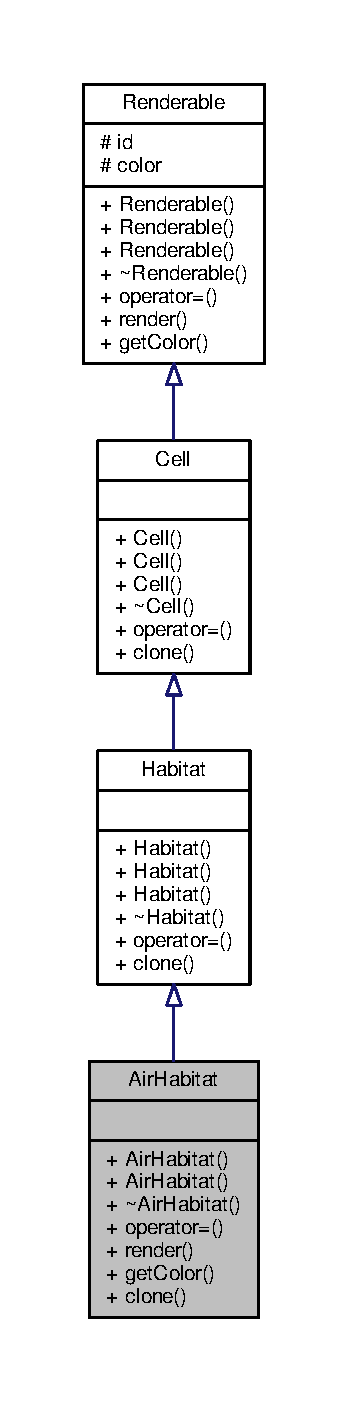
\includegraphics[height=550pt]{classAirHabitat__coll__graph}
\end{center}
\end{figure}
\subsection*{Public Member Functions}
\begin{DoxyCompactItemize}
\item 
\hyperlink{classAirHabitat_aaf82e1201cb35917975fa58ac5a67763}{Air\+Habitat} ()
\begin{DoxyCompactList}\small\item\em Constructor. Menciptakan \hyperlink{classAirHabitat}{Air\+Habitat} kosong. \end{DoxyCompactList}\item 
\hyperlink{classAirHabitat_aaec41ff6acf673890740254b9b47c139}{Air\+Habitat} (const \hyperlink{classAirHabitat}{Air\+Habitat} \&)
\begin{DoxyCompactList}\small\item\em Copy Constructor. Menciptakan salinan dari \hyperlink{classAirHabitat}{Air\+Habitat}. \end{DoxyCompactList}\item 
virtual \hyperlink{classAirHabitat_a18f98f33d3edbb7c397e184f3b7ad56b}{$\sim$\+Air\+Habitat} ()
\begin{DoxyCompactList}\small\item\em Destructor. \end{DoxyCompactList}\item 
\hyperlink{classAirHabitat}{Air\+Habitat} \& \hyperlink{classAirHabitat_a250ef96c8fc2dc62762fcb09819d2098}{operator=} (const \hyperlink{classAirHabitat}{Air\+Habitat} \&)
\begin{DoxyCompactList}\small\item\em Operator=. Menginisialisasi \hyperlink{classAirHabitat}{Air\+Habitat} tanpa terjadi bitwise copy. \end{DoxyCompactList}\item 
char \hyperlink{classAirHabitat_a669080a10d4604141457ba113e5a47e1}{render} ()
\begin{DoxyCompactList}\small\item\em Render. Mengembalikan karakter untuk ditampilkan ke layar. \end{DoxyCompactList}\item 
\hyperlink{color_8h_ab87bacfdad76e61b9412d7124be44c1c}{Color} \hyperlink{classAirHabitat_a098728ad7523cf75ea59f71271a2ace9}{get\+Color} ()
\begin{DoxyCompactList}\small\item\em Get\+Color. Mengembalikan warna untuk ditampilkan ke layar. \end{DoxyCompactList}\item 
virtual \hyperlink{classAirHabitat}{Air\+Habitat} $\ast$ \hyperlink{classAirHabitat_ab756521fcd5adca0283e9bfd0d0fd075}{clone} () const 
\begin{DoxyCompactList}\small\item\em Clone. Menduplikat diri sendiri. \end{DoxyCompactList}\end{DoxyCompactItemize}
\subsection*{Additional Inherited Members}


\subsection{Constructor \& Destructor Documentation}
\index{Air\+Habitat@{Air\+Habitat}!Air\+Habitat@{Air\+Habitat}}
\index{Air\+Habitat@{Air\+Habitat}!Air\+Habitat@{Air\+Habitat}}
\subsubsection[{\texorpdfstring{Air\+Habitat()}{AirHabitat()}}]{\setlength{\rightskip}{0pt plus 5cm}Air\+Habitat\+::\+Air\+Habitat (
\begin{DoxyParamCaption}
{}
\end{DoxyParamCaption}
)}\hypertarget{classAirHabitat_aaf82e1201cb35917975fa58ac5a67763}{}\label{classAirHabitat_aaf82e1201cb35917975fa58ac5a67763}


Constructor. Menciptakan \hyperlink{classAirHabitat}{Air\+Habitat} kosong. 

\index{Air\+Habitat@{Air\+Habitat}!Air\+Habitat@{Air\+Habitat}}
\index{Air\+Habitat@{Air\+Habitat}!Air\+Habitat@{Air\+Habitat}}
\subsubsection[{\texorpdfstring{Air\+Habitat(const Air\+Habitat \&)}{AirHabitat(const AirHabitat &)}}]{\setlength{\rightskip}{0pt plus 5cm}Air\+Habitat\+::\+Air\+Habitat (
\begin{DoxyParamCaption}
\item[{const {\bf Air\+Habitat} \&}]{A}
\end{DoxyParamCaption}
)}\hypertarget{classAirHabitat_aaec41ff6acf673890740254b9b47c139}{}\label{classAirHabitat_aaec41ff6acf673890740254b9b47c139}


Copy Constructor. Menciptakan salinan dari \hyperlink{classAirHabitat}{Air\+Habitat}. 


\begin{DoxyParams}{Parameters}
{\em A} & \hyperlink{classAirHabitat}{Air\+Habitat} yang ingin disalin. \\
\hline
\end{DoxyParams}
\index{Air\+Habitat@{Air\+Habitat}!````~Air\+Habitat@{$\sim$\+Air\+Habitat}}
\index{````~Air\+Habitat@{$\sim$\+Air\+Habitat}!Air\+Habitat@{Air\+Habitat}}
\subsubsection[{\texorpdfstring{$\sim$\+Air\+Habitat()}{~AirHabitat()}}]{\setlength{\rightskip}{0pt plus 5cm}Air\+Habitat\+::$\sim$\+Air\+Habitat (
\begin{DoxyParamCaption}
{}
\end{DoxyParamCaption}
)\hspace{0.3cm}{\ttfamily [virtual]}}\hypertarget{classAirHabitat_a18f98f33d3edbb7c397e184f3b7ad56b}{}\label{classAirHabitat_a18f98f33d3edbb7c397e184f3b7ad56b}


Destructor. 



\subsection{Member Function Documentation}
\index{Air\+Habitat@{Air\+Habitat}!clone@{clone}}
\index{clone@{clone}!Air\+Habitat@{Air\+Habitat}}
\subsubsection[{\texorpdfstring{clone() const }{clone() const }}]{\setlength{\rightskip}{0pt plus 5cm}{\bf Air\+Habitat} $\ast$ Air\+Habitat\+::clone (
\begin{DoxyParamCaption}
{}
\end{DoxyParamCaption}
) const\hspace{0.3cm}{\ttfamily [virtual]}}\hypertarget{classAirHabitat_ab756521fcd5adca0283e9bfd0d0fd075}{}\label{classAirHabitat_ab756521fcd5adca0283e9bfd0d0fd075}


Clone. Menduplikat diri sendiri. 

\begin{DoxyReturn}{Returns}
value object hasil kloning 
\end{DoxyReturn}


Implements \hyperlink{classHabitat_a640c071c99dbd3dc9cbf4971dbcaa463}{Habitat}.

\index{Air\+Habitat@{Air\+Habitat}!get\+Color@{get\+Color}}
\index{get\+Color@{get\+Color}!Air\+Habitat@{Air\+Habitat}}
\subsubsection[{\texorpdfstring{get\+Color()}{getColor()}}]{\setlength{\rightskip}{0pt plus 5cm}{\bf Color} Air\+Habitat\+::get\+Color (
\begin{DoxyParamCaption}
{}
\end{DoxyParamCaption}
)\hspace{0.3cm}{\ttfamily [virtual]}}\hypertarget{classAirHabitat_a098728ad7523cf75ea59f71271a2ace9}{}\label{classAirHabitat_a098728ad7523cf75ea59f71271a2ace9}


Get\+Color. Mengembalikan warna untuk ditampilkan ke layar. 

\begin{DoxyReturn}{Returns}
color warna renderable 
\end{DoxyReturn}


Implements \hyperlink{classRenderable_ab3bcc93b20929c6e92b64223344a73d5}{Renderable}.

\index{Air\+Habitat@{Air\+Habitat}!operator=@{operator=}}
\index{operator=@{operator=}!Air\+Habitat@{Air\+Habitat}}
\subsubsection[{\texorpdfstring{operator=(const Air\+Habitat \&)}{operator=(const AirHabitat &)}}]{\setlength{\rightskip}{0pt plus 5cm}{\bf Air\+Habitat} \& Air\+Habitat\+::operator= (
\begin{DoxyParamCaption}
\item[{const {\bf Air\+Habitat} \&}]{A}
\end{DoxyParamCaption}
)}\hypertarget{classAirHabitat_a250ef96c8fc2dc62762fcb09819d2098}{}\label{classAirHabitat_a250ef96c8fc2dc62762fcb09819d2098}


Operator=. Menginisialisasi \hyperlink{classAirHabitat}{Air\+Habitat} tanpa terjadi bitwise copy. 

\begin{DoxyReturn}{Returns}
\hyperlink{classAirHabitat}{Air\+Habitat} yang sudah di assign nilai dari current object 
\end{DoxyReturn}
\index{Air\+Habitat@{Air\+Habitat}!render@{render}}
\index{render@{render}!Air\+Habitat@{Air\+Habitat}}
\subsubsection[{\texorpdfstring{render()}{render()}}]{\setlength{\rightskip}{0pt plus 5cm}char Air\+Habitat\+::render (
\begin{DoxyParamCaption}
{}
\end{DoxyParamCaption}
)\hspace{0.3cm}{\ttfamily [virtual]}}\hypertarget{classAirHabitat_a669080a10d4604141457ba113e5a47e1}{}\label{classAirHabitat_a669080a10d4604141457ba113e5a47e1}


Render. Mengembalikan karakter untuk ditampilkan ke layar. 

\begin{DoxyReturn}{Returns}
id bertipe char 
\end{DoxyReturn}


Implements \hyperlink{classRenderable_aafa9280e6dcfa557b3cd675221fd97b4}{Renderable}.



The documentation for this class was generated from the following files\+:\begin{DoxyCompactItemize}
\item 
src/renders/habitats/\hyperlink{air__habitat_8h}{air\+\_\+habitat.\+h}\item 
src/renders/habitats/\hyperlink{air__habitat_8cpp}{air\+\_\+habitat.\+cpp}\end{DoxyCompactItemize}

\hypertarget{classAlligator}{}\section{Alligator Class Reference}
\label{classAlligator}\index{Alligator@{Alligator}}


{\ttfamily \#include $<$species.\+h$>$}



Inheritance diagram for Alligator\+:
\nopagebreak
\begin{figure}[H]
\begin{center}
\leavevmode
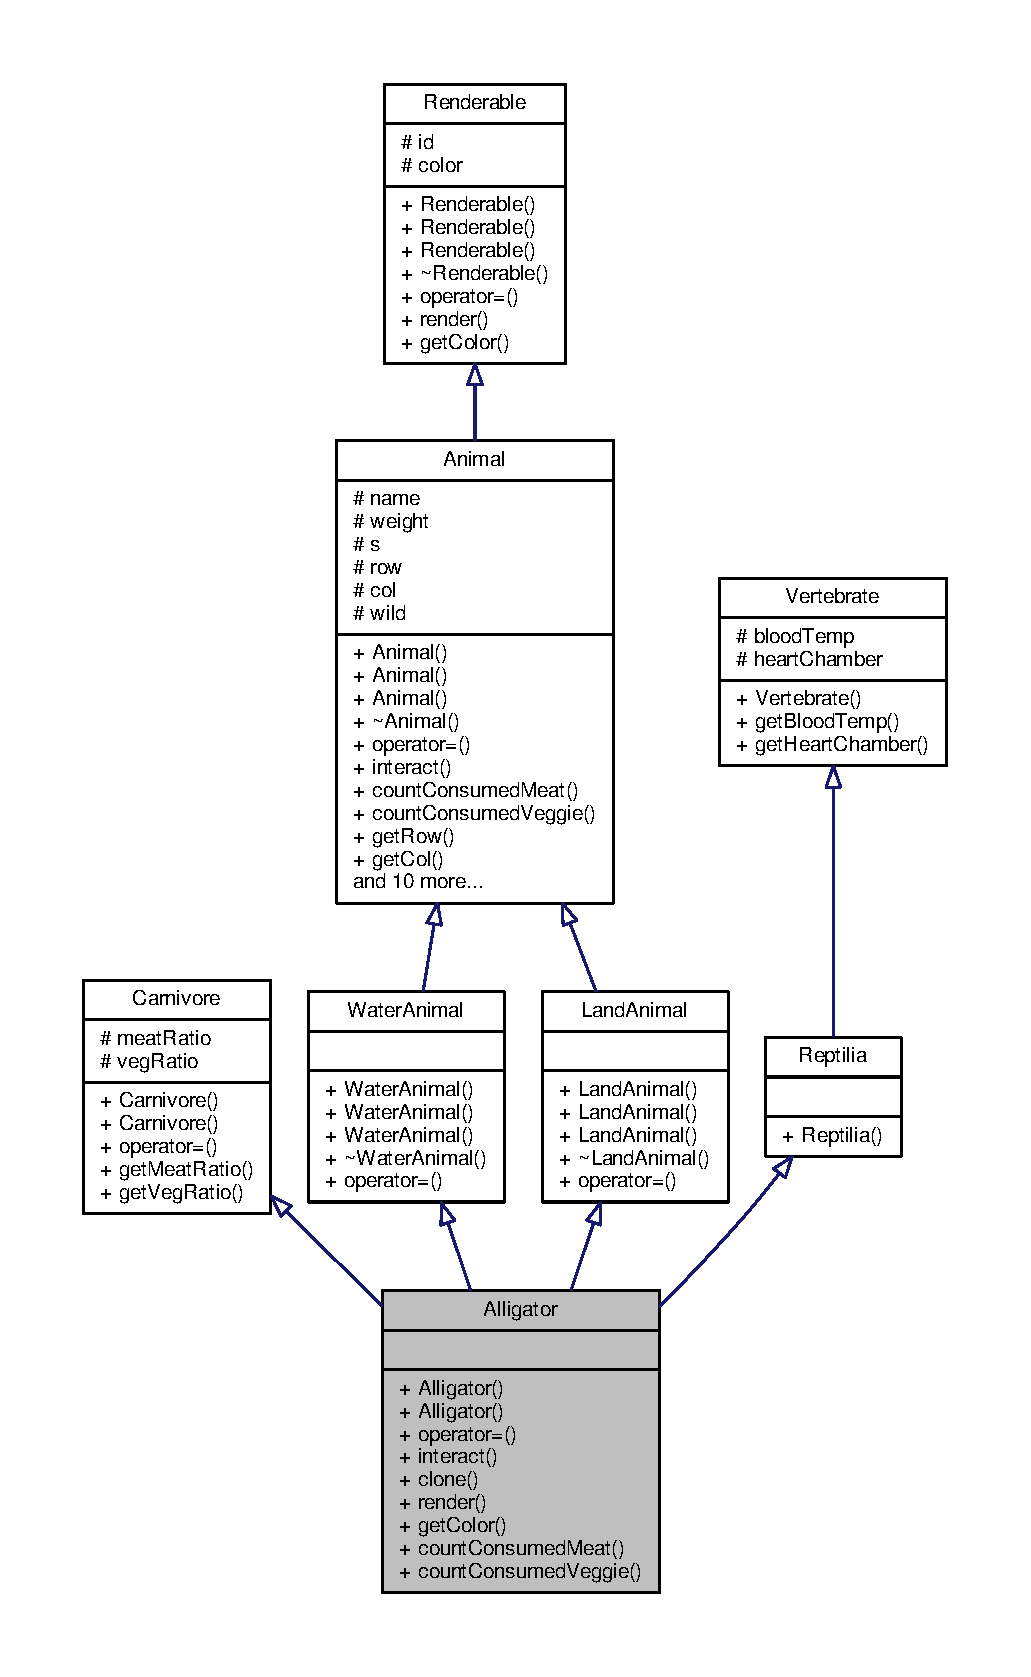
\includegraphics[height=550pt]{classAlligator__inherit__graph}
\end{center}
\end{figure}


Collaboration diagram for Alligator\+:
\nopagebreak
\begin{figure}[H]
\begin{center}
\leavevmode
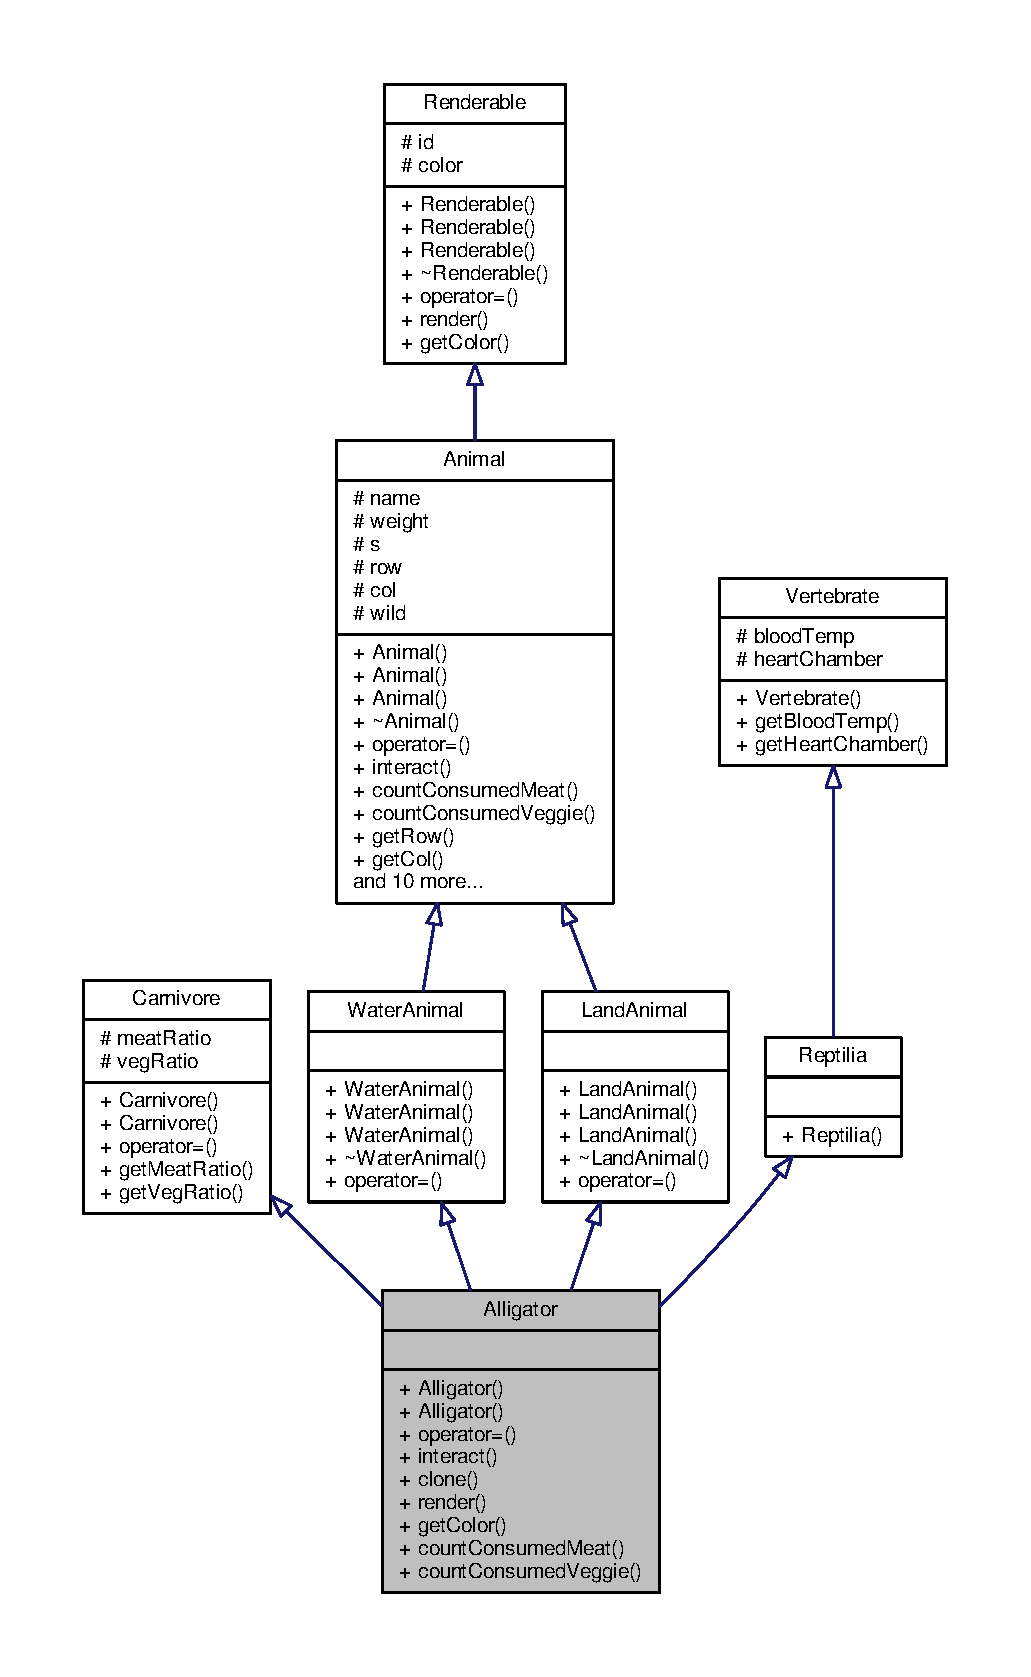
\includegraphics[height=550pt]{classAlligator__coll__graph}
\end{center}
\end{figure}
\subsection*{Public Member Functions}
\begin{DoxyCompactItemize}
\item 
\hyperlink{classAlligator_a394c31cac732c8e80210eb1a08d9be90}{Alligator} (string \+\_\+name, double \+\_\+weight, \hyperlink{sex_8h_a2633cb393c68bb2ee8080db58fb7ba93}{Sex} \+\_\+s, int \+\_\+r, int \+\_\+c)
\begin{DoxyCompactList}\small\item\em Consructor. \end{DoxyCompactList}\item 
\hyperlink{classAlligator_a238834ce335e366454e4720e20471855}{Alligator} (const \hyperlink{classAlligator}{Alligator} \&A)
\begin{DoxyCompactList}\small\item\em Copy Consructor. \end{DoxyCompactList}\item 
\hyperlink{classAlligator}{Alligator} \& \hyperlink{classAlligator_ad264fccaab105b186b2a4dd38e6bb896}{operator=} (const \hyperlink{classAlligator}{Alligator} \&A)
\begin{DoxyCompactList}\small\item\em Operator=. Melakukan assignment pada objek. \end{DoxyCompactList}\item 
virtual void \hyperlink{classAlligator_adad51497aab15fa3ed6cb00bc08ee546}{interact} ()
\begin{DoxyCompactList}\small\item\em interact. Menampilkan interaksi hewan ke layar \end{DoxyCompactList}\item 
virtual \hyperlink{classAlligator}{Alligator} $\ast$ \hyperlink{classAlligator_a307ef9ed05cad69f34b0aa19bc4a4914}{clone} () const 
\begin{DoxyCompactList}\small\item\em clone Menduplikat diri sendiri \end{DoxyCompactList}\item 
virtual char \hyperlink{classAlligator_acc0c14bd7f158137577d158d774efe75}{render} ()
\begin{DoxyCompactList}\small\item\em render Mengembalikan karakter id tiap hewan \end{DoxyCompactList}\item 
virtual \hyperlink{color_8h_ab87bacfdad76e61b9412d7124be44c1c}{Color} \hyperlink{classAlligator_a5bf579134f95113f6a63784622249446}{get\+Color} ()
\begin{DoxyCompactList}\small\item\em get\+Color Mengembalikan warna dari hewan \end{DoxyCompactList}\item 
virtual double \hyperlink{classAlligator_a679001d85f11c97618b9228145a243df}{count\+Consumed\+Meat} ()
\begin{DoxyCompactList}\small\item\em count\+Consumed\+Meat Mengembalikan jumlah daging yang dikonsumsi \end{DoxyCompactList}\item 
virtual double \hyperlink{classAlligator_a5d7511023043e879d8a9aa6f57ada639}{count\+Consumed\+Veggie} ()
\begin{DoxyCompactList}\small\item\em count\+Consumed\+Veggie Mengembalikan jumlah makanan tumbuhan yang dikonsumsi \end{DoxyCompactList}\end{DoxyCompactItemize}
\subsection*{Additional Inherited Members}


\subsection{Constructor \& Destructor Documentation}
\index{Alligator@{Alligator}!Alligator@{Alligator}}
\index{Alligator@{Alligator}!Alligator@{Alligator}}
\subsubsection[{\texorpdfstring{Alligator(string \+\_\+name, double \+\_\+weight, Sex \+\_\+s, int \+\_\+r, int \+\_\+c)}{Alligator(string _name, double _weight, Sex _s, int _r, int _c)}}]{\setlength{\rightskip}{0pt plus 5cm}Alligator\+::\+Alligator (
\begin{DoxyParamCaption}
\item[{string}]{\+\_\+name, }
\item[{double}]{\+\_\+weight, }
\item[{{\bf Sex}}]{\+\_\+s, }
\item[{int}]{\+\_\+r, }
\item[{int}]{\+\_\+c}
\end{DoxyParamCaption}
)}\hypertarget{classAlligator_a394c31cac732c8e80210eb1a08d9be90}{}\label{classAlligator_a394c31cac732c8e80210eb1a08d9be90}


Consructor. 


\begin{DoxyParams}{Parameters}
{\em \+\_\+name} & nama binatang \\
\hline
{\em \+\_\+weight} & berat \\
\hline
{\em \+\_\+s} & jenis kelamin \\
\hline
\end{DoxyParams}
\index{Alligator@{Alligator}!Alligator@{Alligator}}
\index{Alligator@{Alligator}!Alligator@{Alligator}}
\subsubsection[{\texorpdfstring{Alligator(const Alligator \&\+A)}{Alligator(const Alligator &A)}}]{\setlength{\rightskip}{0pt plus 5cm}Alligator\+::\+Alligator (
\begin{DoxyParamCaption}
\item[{const {\bf Alligator} \&}]{A}
\end{DoxyParamCaption}
)}\hypertarget{classAlligator_a238834ce335e366454e4720e20471855}{}\label{classAlligator_a238834ce335e366454e4720e20471855}


Copy Consructor. 


\begin{DoxyParams}{Parameters}
{\em A} & objek yang akan disalin \\
\hline
\end{DoxyParams}


\subsection{Member Function Documentation}
\index{Alligator@{Alligator}!clone@{clone}}
\index{clone@{clone}!Alligator@{Alligator}}
\subsubsection[{\texorpdfstring{clone() const }{clone() const }}]{\setlength{\rightskip}{0pt plus 5cm}{\bf Alligator} $\ast$ Alligator\+::clone (
\begin{DoxyParamCaption}
{}
\end{DoxyParamCaption}
) const\hspace{0.3cm}{\ttfamily [virtual]}}\hypertarget{classAlligator_a307ef9ed05cad69f34b0aa19bc4a4914}{}\label{classAlligator_a307ef9ed05cad69f34b0aa19bc4a4914}


clone Menduplikat diri sendiri 

\begin{DoxyReturn}{Returns}
value object hasil kloning 
\end{DoxyReturn}


Implements \hyperlink{classAnimal_a1430e040ea4ff43bc453fa0ad19c308d}{Animal}.

\index{Alligator@{Alligator}!count\+Consumed\+Meat@{count\+Consumed\+Meat}}
\index{count\+Consumed\+Meat@{count\+Consumed\+Meat}!Alligator@{Alligator}}
\subsubsection[{\texorpdfstring{count\+Consumed\+Meat()}{countConsumedMeat()}}]{\setlength{\rightskip}{0pt plus 5cm}double Alligator\+::count\+Consumed\+Meat (
\begin{DoxyParamCaption}
{}
\end{DoxyParamCaption}
)\hspace{0.3cm}{\ttfamily [virtual]}}\hypertarget{classAlligator_a679001d85f11c97618b9228145a243df}{}\label{classAlligator_a679001d85f11c97618b9228145a243df}


count\+Consumed\+Meat Mengembalikan jumlah daging yang dikonsumsi 

\begin{DoxyReturn}{Returns}
jumlah daging yang dikonsumsi 
\end{DoxyReturn}


Implements \hyperlink{classAnimal_a84ccc380d237650f2bf24d792627d376}{Animal}.

\index{Alligator@{Alligator}!count\+Consumed\+Veggie@{count\+Consumed\+Veggie}}
\index{count\+Consumed\+Veggie@{count\+Consumed\+Veggie}!Alligator@{Alligator}}
\subsubsection[{\texorpdfstring{count\+Consumed\+Veggie()}{countConsumedVeggie()}}]{\setlength{\rightskip}{0pt plus 5cm}double Alligator\+::count\+Consumed\+Veggie (
\begin{DoxyParamCaption}
{}
\end{DoxyParamCaption}
)\hspace{0.3cm}{\ttfamily [virtual]}}\hypertarget{classAlligator_a5d7511023043e879d8a9aa6f57ada639}{}\label{classAlligator_a5d7511023043e879d8a9aa6f57ada639}


count\+Consumed\+Veggie Mengembalikan jumlah makanan tumbuhan yang dikonsumsi 

\begin{DoxyReturn}{Returns}
jumlah makanan tumbuhan yang dikonsumsi 
\end{DoxyReturn}


Implements \hyperlink{classAnimal_aaa7e4bdb7f5a10060b6dcaf09215f822}{Animal}.

\index{Alligator@{Alligator}!get\+Color@{get\+Color}}
\index{get\+Color@{get\+Color}!Alligator@{Alligator}}
\subsubsection[{\texorpdfstring{get\+Color()}{getColor()}}]{\setlength{\rightskip}{0pt plus 5cm}{\bf Color} Alligator\+::get\+Color (
\begin{DoxyParamCaption}
{}
\end{DoxyParamCaption}
)\hspace{0.3cm}{\ttfamily [virtual]}}\hypertarget{classAlligator_a5bf579134f95113f6a63784622249446}{}\label{classAlligator_a5bf579134f95113f6a63784622249446}


get\+Color Mengembalikan warna dari hewan 

\begin{DoxyReturn}{Returns}
warna cetak hewan 
\end{DoxyReturn}


Implements \hyperlink{classRenderable_ab3bcc93b20929c6e92b64223344a73d5}{Renderable}.

\index{Alligator@{Alligator}!interact@{interact}}
\index{interact@{interact}!Alligator@{Alligator}}
\subsubsection[{\texorpdfstring{interact()}{interact()}}]{\setlength{\rightskip}{0pt plus 5cm}void Alligator\+::interact (
\begin{DoxyParamCaption}
{}
\end{DoxyParamCaption}
)\hspace{0.3cm}{\ttfamily [virtual]}}\hypertarget{classAlligator_adad51497aab15fa3ed6cb00bc08ee546}{}\label{classAlligator_adad51497aab15fa3ed6cb00bc08ee546}


interact. Menampilkan interaksi hewan ke layar 



Implements \hyperlink{classAnimal_af47626b050b665e9a19525227d2b840f}{Animal}.

\index{Alligator@{Alligator}!operator=@{operator=}}
\index{operator=@{operator=}!Alligator@{Alligator}}
\subsubsection[{\texorpdfstring{operator=(const Alligator \&\+A)}{operator=(const Alligator &A)}}]{\setlength{\rightskip}{0pt plus 5cm}{\bf Alligator} \& Alligator\+::operator= (
\begin{DoxyParamCaption}
\item[{const {\bf Alligator} \&}]{A}
\end{DoxyParamCaption}
)}\hypertarget{classAlligator_ad264fccaab105b186b2a4dd38e6bb896}{}\label{classAlligator_ad264fccaab105b186b2a4dd38e6bb896}


Operator=. Melakukan assignment pada objek. 


\begin{DoxyParams}{Parameters}
{\em A} & objek yang akan disalin \\
\hline
\end{DoxyParams}
\index{Alligator@{Alligator}!render@{render}}
\index{render@{render}!Alligator@{Alligator}}
\subsubsection[{\texorpdfstring{render()}{render()}}]{\setlength{\rightskip}{0pt plus 5cm}char Alligator\+::render (
\begin{DoxyParamCaption}
{}
\end{DoxyParamCaption}
)\hspace{0.3cm}{\ttfamily [virtual]}}\hypertarget{classAlligator_acc0c14bd7f158137577d158d774efe75}{}\label{classAlligator_acc0c14bd7f158137577d158d774efe75}


render Mengembalikan karakter id tiap hewan 

\begin{DoxyReturn}{Returns}
karakter tiap hewan 
\end{DoxyReturn}


Implements \hyperlink{classRenderable_aafa9280e6dcfa557b3cd675221fd97b4}{Renderable}.



The documentation for this class was generated from the following files\+:\begin{DoxyCompactItemize}
\item 
src/renders/animals/\hyperlink{species_8h}{species.\+h}\item 
src/renders/animals/\hyperlink{species_8cpp}{species.\+cpp}\end{DoxyCompactItemize}

\hypertarget{classAmphibia}{}\section{Amphibia Class Reference}
\label{classAmphibia}\index{Amphibia@{Amphibia}}


{\ttfamily \#include $<$amphibia.\+h$>$}



Inheritance diagram for Amphibia\+:
\nopagebreak
\begin{figure}[H]
\begin{center}
\leavevmode
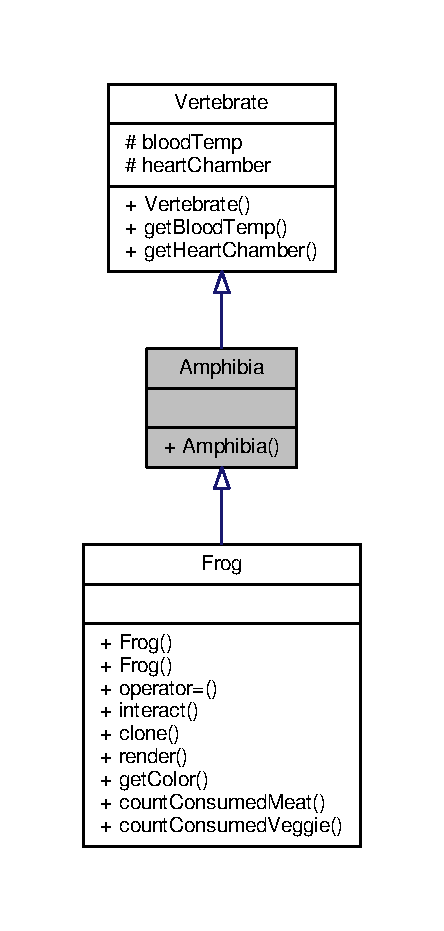
\includegraphics[width=213pt]{classAmphibia__inherit__graph}
\end{center}
\end{figure}


Collaboration diagram for Amphibia\+:
\nopagebreak
\begin{figure}[H]
\begin{center}
\leavevmode
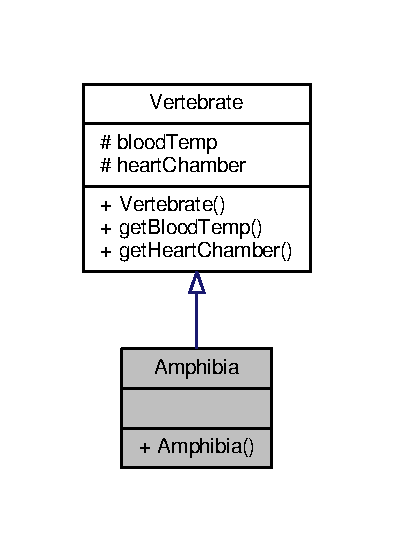
\includegraphics[width=189pt]{classAmphibia__coll__graph}
\end{center}
\end{figure}
\subsection*{Public Member Functions}
\begin{DoxyCompactItemize}
\item 
\hyperlink{classAmphibia_ae1a692326c911b131cee2fbb615a9786}{Amphibia} ()
\begin{DoxyCompactList}\small\item\em Constructor. \end{DoxyCompactList}\end{DoxyCompactItemize}
\subsection*{Additional Inherited Members}


\subsection{Detailed Description}
Kelas taksonomi untuk amphibi 

\subsection{Constructor \& Destructor Documentation}
\index{Amphibia@{Amphibia}!Amphibia@{Amphibia}}
\index{Amphibia@{Amphibia}!Amphibia@{Amphibia}}
\subsubsection[{\texorpdfstring{Amphibia()}{Amphibia()}}]{\setlength{\rightskip}{0pt plus 5cm}Amphibia\+::\+Amphibia (
\begin{DoxyParamCaption}
{}
\end{DoxyParamCaption}
)}\hypertarget{classAmphibia_ae1a692326c911b131cee2fbb615a9786}{}\label{classAmphibia_ae1a692326c911b131cee2fbb615a9786}


Constructor. 



The documentation for this class was generated from the following files\+:\begin{DoxyCompactItemize}
\item 
src/renders/animals/taxonomy/\hyperlink{amphibia_8h}{amphibia.\+h}\item 
src/renders/animals/taxonomy/\hyperlink{amphibia_8cpp}{amphibia.\+cpp}\end{DoxyCompactItemize}

\hypertarget{classAnimal}{}\section{Animal Class Reference}
\label{classAnimal}\index{Animal@{Animal}}


{\ttfamily \#include $<$animal.\+h$>$}



Inheritance diagram for Animal\+:
\nopagebreak
\begin{figure}[H]
\begin{center}
\leavevmode
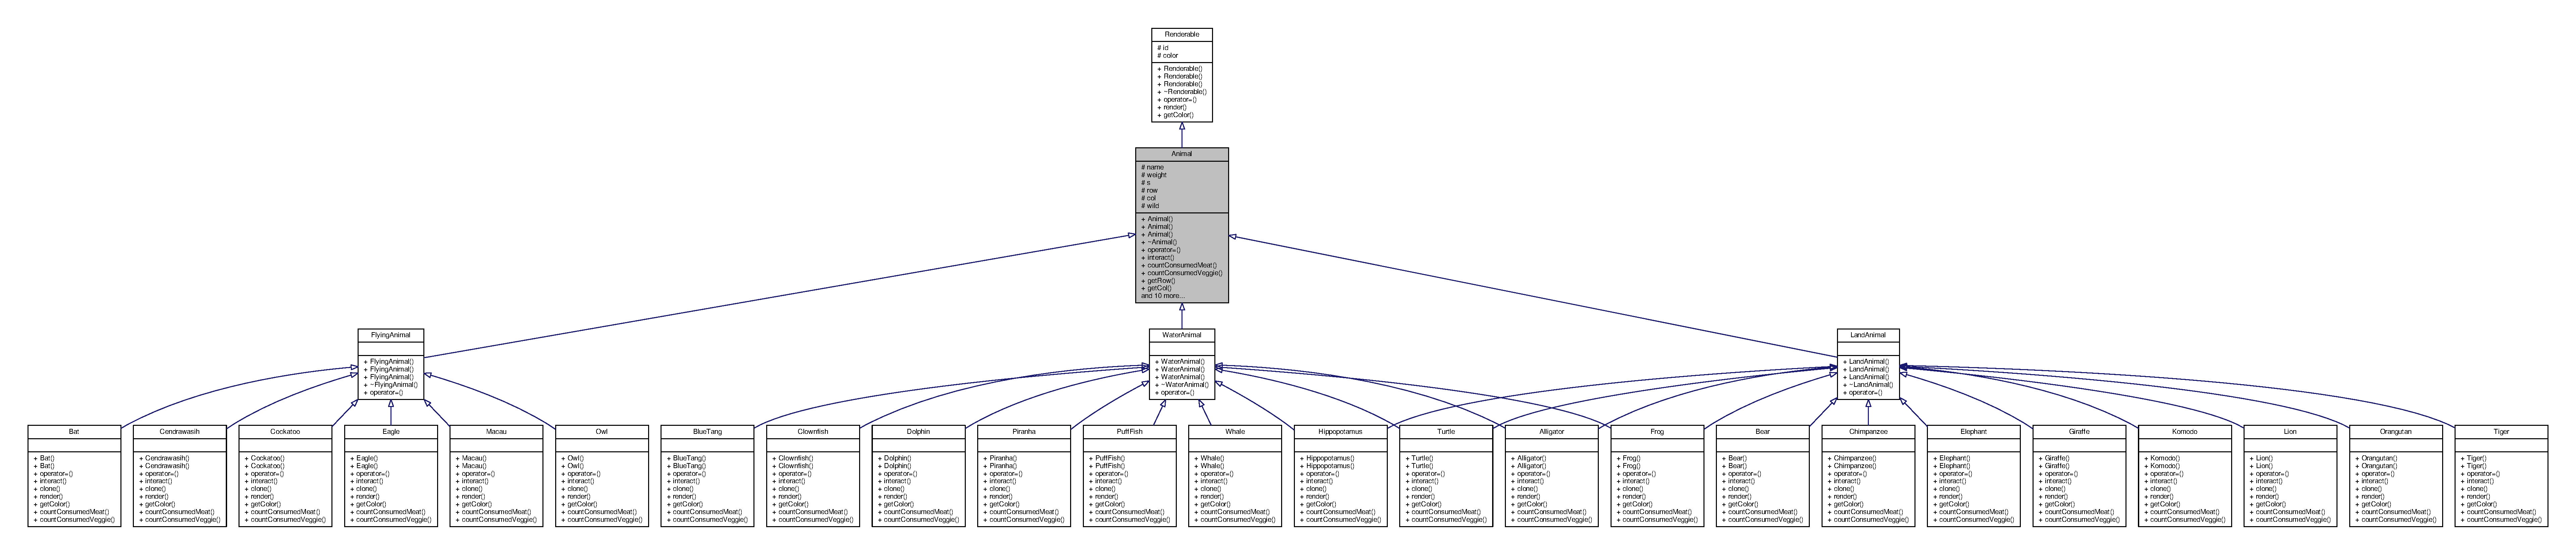
\includegraphics[width=350pt]{classAnimal__inherit__graph}
\end{center}
\end{figure}


Collaboration diagram for Animal\+:
\nopagebreak
\begin{figure}[H]
\begin{center}
\leavevmode
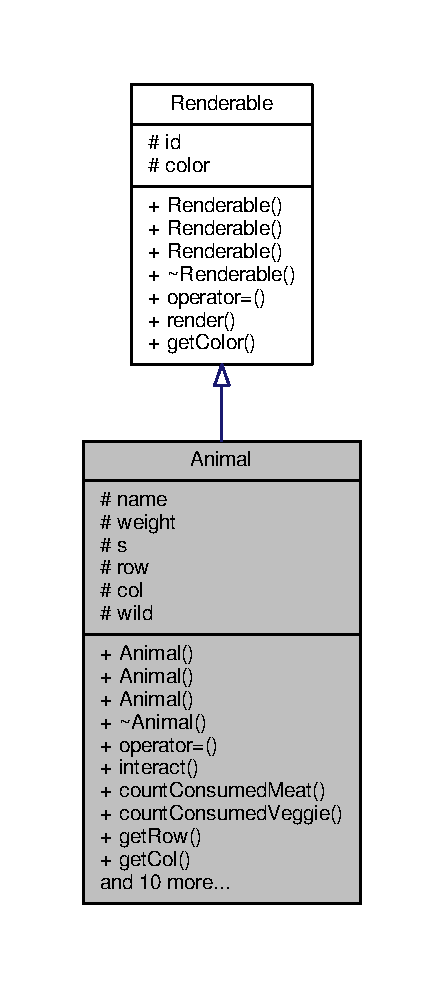
\includegraphics[width=213pt]{classAnimal__coll__graph}
\end{center}
\end{figure}
\subsection*{Public Member Functions}
\begin{DoxyCompactItemize}
\item 
\hyperlink{classAnimal_a1e726a49ec952443190ac62dad22353c}{Animal} ()
\begin{DoxyCompactList}\small\item\em Constructor. \end{DoxyCompactList}\item 
\hyperlink{classAnimal_a84c6d203680b00cb07f2ec48f680ed45}{Animal} (std\+::string \+\_\+name, double \+\_\+weight, \hyperlink{sex_8h_a2633cb393c68bb2ee8080db58fb7ba93}{Sex} \+\_\+s, int \+\_\+r, int \+\_\+c, char \+\_\+id, \hyperlink{color_8h_ab87bacfdad76e61b9412d7124be44c1c}{Color} \+\_\+color, bool \+\_\+w)
\begin{DoxyCompactList}\small\item\em Constructor. \end{DoxyCompactList}\item 
\hyperlink{classAnimal_a97b35f0ad64b9a45c24330d47a164c84}{Animal} (const \hyperlink{classAnimal}{Animal} \&A)
\begin{DoxyCompactList}\small\item\em Copy Constructor. \end{DoxyCompactList}\item 
virtual \hyperlink{classAnimal_a476af25adde5f0dfa688129c8f86fa5c}{$\sim$\+Animal} ()
\begin{DoxyCompactList}\small\item\em Destructor. \end{DoxyCompactList}\item 
\hyperlink{classAnimal}{Animal} \& \hyperlink{classAnimal_a57ae10591202bc5bcc5df2af25d63b34}{operator=} (const \hyperlink{classAnimal}{Animal} \&A)
\begin{DoxyCompactList}\small\item\em Operator= Menjamin bukan bitwise copy. \end{DoxyCompactList}\item 
virtual void \hyperlink{classAnimal_af47626b050b665e9a19525227d2b840f}{interact} ()=0
\begin{DoxyCompactList}\small\item\em Menampilkan experience yang dialami pengamat dengan hewan. Adalah fungsi virtual murni, diimplementasikan oleh kelas anaknya. \end{DoxyCompactList}\item 
virtual double \hyperlink{classAnimal_a84ccc380d237650f2bf24d792627d376}{count\+Consumed\+Meat} ()=0
\begin{DoxyCompactList}\small\item\em Menghitung jumlah daging yang dikonsumsi Adalah fungsi virtual murni, diimplementasikan oleh kelas anaknya. \end{DoxyCompactList}\item 
virtual double \hyperlink{classAnimal_aaa7e4bdb7f5a10060b6dcaf09215f822}{count\+Consumed\+Veggie} ()=0
\begin{DoxyCompactList}\small\item\em Menghitung jumlah tumbuhan yang dikonsumsi Adalah fungsi virtual murni, diimplementasikan oleh kelas anaknya. \end{DoxyCompactList}\item 
int \hyperlink{classAnimal_aa3c07c4eea7541a53c0b3b1ab60ee823}{get\+Row} () const 
\begin{DoxyCompactList}\small\item\em Mengembalikan jumlah baris. \end{DoxyCompactList}\item 
int \hyperlink{classAnimal_a8d5109b00432d23c5d92994f16f7f4d3}{get\+Col} () const 
\begin{DoxyCompactList}\small\item\em Mengembalikan jumlah kolom. \end{DoxyCompactList}\item 
double \hyperlink{classAnimal_a236f28ce33ff9d88b19289decf04e85d}{get\+Weight} () const 
\begin{DoxyCompactList}\small\item\em Mengembalikan berat hewan. \end{DoxyCompactList}\item 
string \hyperlink{classAnimal_a1b2cd74cdd5dee4f3673515bf7672a61}{get\+Name} () const 
\begin{DoxyCompactList}\small\item\em get\+Name Mengembalikan nama hewan \end{DoxyCompactList}\item 
\hyperlink{sex_8h_a2633cb393c68bb2ee8080db58fb7ba93}{Sex} \hyperlink{classAnimal_ab893137840cdbcc79bf37d1917fdb07d}{get\+Sex} () const 
\begin{DoxyCompactList}\small\item\em Mengembalikan jenis kelamin hewan. \end{DoxyCompactList}\item 
bool \hyperlink{classAnimal_ae2db41292da71f0d97f0f14b89e9ca54}{get\+Wild} () const 
\begin{DoxyCompactList}\small\item\em Mengembalikan T\+R\+UE bila hewan tidak jinak. \end{DoxyCompactList}\item 
void \hyperlink{classAnimal_a4b671d61e51b5571b2c970cfbeacec83}{set\+Row} (int r)
\begin{DoxyCompactList}\small\item\em Mengatur posisi baris hewan. \end{DoxyCompactList}\item 
void \hyperlink{classAnimal_a6605290f0ff9a1db578fb11dff721961}{set\+Col} (int c)
\begin{DoxyCompactList}\small\item\em Mengatur posisi kolom hewan. \end{DoxyCompactList}\item 
void \hyperlink{classAnimal_a0472ed25f9cc47d45729dc530088c3ae}{set\+Weight} (double w)
\begin{DoxyCompactList}\small\item\em Mengatur berat hewan. \end{DoxyCompactList}\item 
void \hyperlink{classAnimal_aa26d5b8f6912f03da2cc64ff0b888972}{set\+Name} (string n)
\begin{DoxyCompactList}\small\item\em Mengatur nama hewan. \end{DoxyCompactList}\item 
void \hyperlink{classAnimal_a6ed9f74c98160a980ef0666ecf5f9014}{set\+Sex} (\hyperlink{sex_8h_a2633cb393c68bb2ee8080db58fb7ba93}{Sex} ns)
\begin{DoxyCompactList}\small\item\em Mengatur jenis kelamin hewan. \end{DoxyCompactList}\item 
virtual \hyperlink{classAnimal}{Animal} $\ast$ \hyperlink{classAnimal_a1430e040ea4ff43bc453fa0ad19c308d}{clone} () const =0
\begin{DoxyCompactList}\small\item\em Menduplikasi \hyperlink{classAnimal}{Animal} tanpa terjadi bitwise copy. \end{DoxyCompactList}\end{DoxyCompactItemize}
\subsection*{Protected Attributes}
\begin{DoxyCompactItemize}
\item 
string \hyperlink{classAnimal_a9cf3bfd9070daec7b3bbc87cbd958f35}{name}
\item 
double \hyperlink{classAnimal_a65e900977918b50f9e5ff534dc1e8c01}{weight}
\item 
\hyperlink{sex_8h_a2633cb393c68bb2ee8080db58fb7ba93}{Sex} \hyperlink{classAnimal_a69cdeeac01d5b83eb441aacb5be935f1}{s}
\item 
int \hyperlink{classAnimal_a3eabc10dd98963d59485be78dc49fd86}{row}
\item 
int \hyperlink{classAnimal_a31aa34abac8c22b898aef97ca63f2630}{col}
\item 
bool \hyperlink{classAnimal_a6228996b6df852e6db2776c07c084afe}{wild}
\end{DoxyCompactItemize}
\subsection*{Friends}
\begin{DoxyCompactItemize}
\item 
istream \& \hyperlink{classAnimal_ae1c2dc52641f7001abeabd267e1a7dc9}{operator$>$$>$} (istream \&in, \hyperlink{classAnimal}{Animal} $\ast$\&A)
\begin{DoxyCompactList}\small\item\em Operator$>$$>$ \end{DoxyCompactList}\item 
ostream \& \hyperlink{classAnimal_a4d6786d5c8d30ed0c8047321ab47b5ff}{operator$<$$<$} (ostream \&os, \hyperlink{classAnimal}{Animal} \&A)
\begin{DoxyCompactList}\small\item\em operator$<$$<$ Mencetak informasi dari hewan \end{DoxyCompactList}\end{DoxyCompactItemize}


\subsection{Detailed Description}
Adalah kelas anak dari \hyperlink{classRenderable}{Renderable} karena \hyperlink{classAnimal}{Animal} dapat dicetak. Adalah kelas yang memiliki metode dan atribut binatang. 

\subsection{Constructor \& Destructor Documentation}
\index{Animal@{Animal}!Animal@{Animal}}
\index{Animal@{Animal}!Animal@{Animal}}
\subsubsection[{\texorpdfstring{Animal()}{Animal()}}]{\setlength{\rightskip}{0pt plus 5cm}Animal\+::\+Animal (
\begin{DoxyParamCaption}
{}
\end{DoxyParamCaption}
)}\hypertarget{classAnimal_a1e726a49ec952443190ac62dad22353c}{}\label{classAnimal_a1e726a49ec952443190ac62dad22353c}


Constructor. 

\index{Animal@{Animal}!Animal@{Animal}}
\index{Animal@{Animal}!Animal@{Animal}}
\subsubsection[{\texorpdfstring{Animal(std\+::string \+\_\+name, double \+\_\+weight, Sex \+\_\+s, int \+\_\+r, int \+\_\+c, char \+\_\+id, Color \+\_\+color, bool \+\_\+w)}{Animal(std::string _name, double _weight, Sex _s, int _r, int _c, char _id, Color _color, bool _w)}}]{\setlength{\rightskip}{0pt plus 5cm}Animal\+::\+Animal (
\begin{DoxyParamCaption}
\item[{std\+::string}]{\+\_\+name, }
\item[{double}]{\+\_\+weight, }
\item[{{\bf Sex}}]{\+\_\+s, }
\item[{int}]{\+\_\+r, }
\item[{int}]{\+\_\+c, }
\item[{char}]{\+\_\+id, }
\item[{{\bf Color}}]{\+\_\+color, }
\item[{bool}]{\+\_\+w}
\end{DoxyParamCaption}
)}\hypertarget{classAnimal_a84c6d203680b00cb07f2ec48f680ed45}{}\label{classAnimal_a84c6d203680b00cb07f2ec48f680ed45}


Constructor. 


\begin{DoxyParams}{Parameters}
{\em \+\_\+name} & nama binatang \\
\hline
{\em \+\_\+weight} & berat binatang \\
\hline
{\em \+\_\+s} & jenis kelamin \\
\hline
\end{DoxyParams}
\index{Animal@{Animal}!Animal@{Animal}}
\index{Animal@{Animal}!Animal@{Animal}}
\subsubsection[{\texorpdfstring{Animal(const Animal \&\+A)}{Animal(const Animal &A)}}]{\setlength{\rightskip}{0pt plus 5cm}Animal\+::\+Animal (
\begin{DoxyParamCaption}
\item[{const {\bf Animal} \&}]{A}
\end{DoxyParamCaption}
)}\hypertarget{classAnimal_a97b35f0ad64b9a45c24330d47a164c84}{}\label{classAnimal_a97b35f0ad64b9a45c24330d47a164c84}


Copy Constructor. 


\begin{DoxyParams}{Parameters}
{\em \hyperlink{classAnimal}{Animal}} & A yang ingin disalin. \\
\hline
\end{DoxyParams}
\index{Animal@{Animal}!````~Animal@{$\sim$\+Animal}}
\index{````~Animal@{$\sim$\+Animal}!Animal@{Animal}}
\subsubsection[{\texorpdfstring{$\sim$\+Animal()}{~Animal()}}]{\setlength{\rightskip}{0pt plus 5cm}Animal\+::$\sim$\+Animal (
\begin{DoxyParamCaption}
{}
\end{DoxyParamCaption}
)\hspace{0.3cm}{\ttfamily [virtual]}}\hypertarget{classAnimal_a476af25adde5f0dfa688129c8f86fa5c}{}\label{classAnimal_a476af25adde5f0dfa688129c8f86fa5c}


Destructor. 



\subsection{Member Function Documentation}
\index{Animal@{Animal}!clone@{clone}}
\index{clone@{clone}!Animal@{Animal}}
\subsubsection[{\texorpdfstring{clone() const =0}{clone() const =0}}]{\setlength{\rightskip}{0pt plus 5cm}virtual {\bf Animal}$\ast$ Animal\+::clone (
\begin{DoxyParamCaption}
{}
\end{DoxyParamCaption}
) const\hspace{0.3cm}{\ttfamily [pure virtual]}}\hypertarget{classAnimal_a1430e040ea4ff43bc453fa0ad19c308d}{}\label{classAnimal_a1430e040ea4ff43bc453fa0ad19c308d}


Menduplikasi \hyperlink{classAnimal}{Animal} tanpa terjadi bitwise copy. 

\begin{DoxyReturn}{Returns}
\hyperlink{classAnimal}{Animal} yang sudah diduplikasi. 
\end{DoxyReturn}


Implemented in \hyperlink{classTurtle_ae63e85cb0508d8cf7a254d8d02b05bf5}{Turtle}, \hyperlink{classHippopotamus_ae332973578e7a9a8bfde9cd7fb972d5e}{Hippopotamus}, \hyperlink{classAlligator_a307ef9ed05cad69f34b0aa19bc4a4914}{Alligator}, \hyperlink{classFrog_aab84684c4f6729ab89b1dd7470471d06}{Frog}, \hyperlink{classCockatoo_ad679253fde6f461fa49011583d113d48}{Cockatoo}, \hyperlink{classMacau_a66cffd38f3eeb221344a52b62591a06e}{Macau}, \hyperlink{classBat_a424595b4e6c12819cc4b1a4083c756cb}{Bat}, \hyperlink{classOwl_a2bb2b61736ff978ec96223cc67ba2dfa}{Owl}, \hyperlink{classCendrawasih_a39cf4d2c4a8008a0d6e1292f1cbb86b2}{Cendrawasih}, \hyperlink{classEagle_a8b6f062eccca508c551b27c1581e7d83}{Eagle}, \hyperlink{classPuffFish_a4e8098eefcedd557fe9e490646ef14d9}{Puff\+Fish}, \hyperlink{classPiranha_a7f844252f5836441f77dc90e12822813}{Piranha}, \hyperlink{classBlueTang_a2b4ac8cf3cddaa66c9cc361c6cc3361b}{Blue\+Tang}, \hyperlink{classClownfish_aa4ee84fc66ce7a63aa8a8d64abb26de5}{Clownfish}, \hyperlink{classDolphin_a77c541ea19646ec22a5461cb9788ccb6}{Dolphin}, \hyperlink{classWhale_afaae0fbf8fa68bb122a8b977e174991b}{Whale}, \hyperlink{classBear_a72baa5599585a59e57727f0f00e09e60}{Bear}, \hyperlink{classKomodo_a2b1b5b9e53444eb2aa9ac0784a492bae}{Komodo}, \hyperlink{classChimpanzee_ab4e4e896ca7461d22c526e5a86602903}{Chimpanzee}, \hyperlink{classOrangutan_a58ca36d261bc661415f82c751f6d24b0}{Orangutan}, \hyperlink{classTiger_a9c253adc25d2ecf06da155a402e5437c}{Tiger}, \hyperlink{classLion_a7c094b9988d5d1dae6136bca49f3b91b}{Lion}, \hyperlink{classGiraffe_a37a4621ceb9515e1069a691971c4a31b}{Giraffe}, and \hyperlink{classElephant_a5f3470439cfb819eb68a8ebc070ffaee}{Elephant}.

\index{Animal@{Animal}!count\+Consumed\+Meat@{count\+Consumed\+Meat}}
\index{count\+Consumed\+Meat@{count\+Consumed\+Meat}!Animal@{Animal}}
\subsubsection[{\texorpdfstring{count\+Consumed\+Meat()=0}{countConsumedMeat()=0}}]{\setlength{\rightskip}{0pt plus 5cm}virtual double Animal\+::count\+Consumed\+Meat (
\begin{DoxyParamCaption}
{}
\end{DoxyParamCaption}
)\hspace{0.3cm}{\ttfamily [pure virtual]}}\hypertarget{classAnimal_a84ccc380d237650f2bf24d792627d376}{}\label{classAnimal_a84ccc380d237650f2bf24d792627d376}


Menghitung jumlah daging yang dikonsumsi Adalah fungsi virtual murni, diimplementasikan oleh kelas anaknya. 

\begin{DoxyReturn}{Returns}
jumlah daging yang dikonsumsi 
\end{DoxyReturn}


Implemented in \hyperlink{classTurtle_a19ac999a6f58e77680581ce45effa577}{Turtle}, \hyperlink{classHippopotamus_a55db3d0400a34c50b9dbf8718d31980c}{Hippopotamus}, \hyperlink{classAlligator_a679001d85f11c97618b9228145a243df}{Alligator}, \hyperlink{classFrog_a5297e5e8eebab6d3f67c36e318db56fe}{Frog}, \hyperlink{classCockatoo_a1a0ef8c860f34aee56cecd982e8d8c4b}{Cockatoo}, \hyperlink{classMacau_aa02eae75670d3206147b4702bc5b70be}{Macau}, \hyperlink{classBat_a99a15e819b635da5f3342189d02399a2}{Bat}, \hyperlink{classOwl_ad17ff8e684fbf199bb191e3ecb6e3e37}{Owl}, \hyperlink{classCendrawasih_a899bcc2043226dc51f77f02c644f7c3f}{Cendrawasih}, \hyperlink{classEagle_a815be21cd5e4e1716a36c39eda33b686}{Eagle}, \hyperlink{classPuffFish_a4e3b5bc7adbe6a683fbe0ec03c00ea0c}{Puff\+Fish}, \hyperlink{classPiranha_a7dbc301f51652df5cbba42896ba4b54b}{Piranha}, \hyperlink{classBlueTang_abb9f72532beeac89a07db47010b5124b}{Blue\+Tang}, \hyperlink{classClownfish_a891dd1c6ccb470273d37f4a39bfbfea8}{Clownfish}, \hyperlink{classDolphin_a6c53ee214a0092e13417645b16387596}{Dolphin}, \hyperlink{classWhale_a0b35a77b6aaea6b15ebc93d854fbb41d}{Whale}, \hyperlink{classBear_ac4919e42fe08c1ec792abac72de24f1f}{Bear}, \hyperlink{classKomodo_a3625afd11c1b671636f4e5bd78cf2101}{Komodo}, \hyperlink{classChimpanzee_a7890d585fe43b40b65c5ac68c02bc1a8}{Chimpanzee}, \hyperlink{classOrangutan_afd19f58f4c885084e833f20cef147805}{Orangutan}, \hyperlink{classTiger_a049d69f6adde018719d8a661c22cd3de}{Tiger}, \hyperlink{classLion_a3ab5c2ab285a4f098a1d37eba7624f01}{Lion}, \hyperlink{classGiraffe_a18d770d4819d5c82ef9887a546765c89}{Giraffe}, and \hyperlink{classElephant_ab210c0612d4e9ab539dc47a0776a8997}{Elephant}.

\index{Animal@{Animal}!count\+Consumed\+Veggie@{count\+Consumed\+Veggie}}
\index{count\+Consumed\+Veggie@{count\+Consumed\+Veggie}!Animal@{Animal}}
\subsubsection[{\texorpdfstring{count\+Consumed\+Veggie()=0}{countConsumedVeggie()=0}}]{\setlength{\rightskip}{0pt plus 5cm}virtual double Animal\+::count\+Consumed\+Veggie (
\begin{DoxyParamCaption}
{}
\end{DoxyParamCaption}
)\hspace{0.3cm}{\ttfamily [pure virtual]}}\hypertarget{classAnimal_aaa7e4bdb7f5a10060b6dcaf09215f822}{}\label{classAnimal_aaa7e4bdb7f5a10060b6dcaf09215f822}


Menghitung jumlah tumbuhan yang dikonsumsi Adalah fungsi virtual murni, diimplementasikan oleh kelas anaknya. 

\begin{DoxyReturn}{Returns}
jumlah tumbuhan yang dikonsumsi 
\end{DoxyReturn}


Implemented in \hyperlink{classTurtle_a663df986cfd11e65d96e9796c803617f}{Turtle}, \hyperlink{classHippopotamus_abf66ac77f92d82a60b76424e25fdd2fe}{Hippopotamus}, \hyperlink{classAlligator_a5d7511023043e879d8a9aa6f57ada639}{Alligator}, \hyperlink{classFrog_a0e6b1ee5d8a1dee1adde9ca4f3c7367e}{Frog}, \hyperlink{classCockatoo_a757745e9991110e16036d48f8468bbf5}{Cockatoo}, \hyperlink{classMacau_a423bd20b9c222540b146f9a783a82562}{Macau}, \hyperlink{classBat_a496ea2d647757518276d20a12d3dea44}{Bat}, \hyperlink{classOwl_ad8c5f218317a583204300a3ad353442b}{Owl}, \hyperlink{classCendrawasih_ae3e380084d6e7e9574d2bdb439155ccc}{Cendrawasih}, \hyperlink{classEagle_a5f27f80f81ed438bf9de8a84c24765fb}{Eagle}, \hyperlink{classPuffFish_a356a72134c1005851ffd5ee8d71a296c}{Puff\+Fish}, \hyperlink{classPiranha_a78ae3e98577fe780b1d768a08632df67}{Piranha}, \hyperlink{classBlueTang_abab5b6bae1d54d9c059076f19cd1f3af}{Blue\+Tang}, \hyperlink{classClownfish_ad7c3808e5d5b7ec463e80447b505886b}{Clownfish}, \hyperlink{classDolphin_a528ae87e039dcb252d90815e37535eb9}{Dolphin}, \hyperlink{classWhale_ab11932aef7e81d1013eaf4a12ab835b3}{Whale}, \hyperlink{classBear_a58587a79a0b4df2a7d9629948f339c90}{Bear}, \hyperlink{classKomodo_a00e61d238ddb66453c335f6fa340385d}{Komodo}, \hyperlink{classChimpanzee_a8a9a0561d0eacc5c82fad0ea4e4ed99d}{Chimpanzee}, \hyperlink{classOrangutan_a1ce87d81f98728217b3e500034bc738e}{Orangutan}, \hyperlink{classTiger_aa1cfc0f2b4923202857925c699084cc3}{Tiger}, \hyperlink{classLion_adcd29cbbaf55e6a930271980406e725d}{Lion}, \hyperlink{classGiraffe_ac998c481a5228750394bb8929174c618}{Giraffe}, and \hyperlink{classElephant_a2919bc91970a375001341d63526590c5}{Elephant}.

\index{Animal@{Animal}!get\+Col@{get\+Col}}
\index{get\+Col@{get\+Col}!Animal@{Animal}}
\subsubsection[{\texorpdfstring{get\+Col() const }{getCol() const }}]{\setlength{\rightskip}{0pt plus 5cm}int Animal\+::get\+Col (
\begin{DoxyParamCaption}
{}
\end{DoxyParamCaption}
) const}\hypertarget{classAnimal_a8d5109b00432d23c5d92994f16f7f4d3}{}\label{classAnimal_a8d5109b00432d23c5d92994f16f7f4d3}


Mengembalikan jumlah kolom. 

\begin{DoxyReturn}{Returns}
jumlah kolom 
\end{DoxyReturn}
\index{Animal@{Animal}!get\+Name@{get\+Name}}
\index{get\+Name@{get\+Name}!Animal@{Animal}}
\subsubsection[{\texorpdfstring{get\+Name() const }{getName() const }}]{\setlength{\rightskip}{0pt plus 5cm}string Animal\+::get\+Name (
\begin{DoxyParamCaption}
{}
\end{DoxyParamCaption}
) const}\hypertarget{classAnimal_a1b2cd74cdd5dee4f3673515bf7672a61}{}\label{classAnimal_a1b2cd74cdd5dee4f3673515bf7672a61}


get\+Name Mengembalikan nama hewan 

\begin{DoxyReturn}{Returns}
nama hewan 
\end{DoxyReturn}
\index{Animal@{Animal}!get\+Row@{get\+Row}}
\index{get\+Row@{get\+Row}!Animal@{Animal}}
\subsubsection[{\texorpdfstring{get\+Row() const }{getRow() const }}]{\setlength{\rightskip}{0pt plus 5cm}int Animal\+::get\+Row (
\begin{DoxyParamCaption}
{}
\end{DoxyParamCaption}
) const}\hypertarget{classAnimal_aa3c07c4eea7541a53c0b3b1ab60ee823}{}\label{classAnimal_aa3c07c4eea7541a53c0b3b1ab60ee823}


Mengembalikan jumlah baris. 

\begin{DoxyReturn}{Returns}
jumlah baris 
\end{DoxyReturn}
\index{Animal@{Animal}!get\+Sex@{get\+Sex}}
\index{get\+Sex@{get\+Sex}!Animal@{Animal}}
\subsubsection[{\texorpdfstring{get\+Sex() const }{getSex() const }}]{\setlength{\rightskip}{0pt plus 5cm}{\bf Sex} Animal\+::get\+Sex (
\begin{DoxyParamCaption}
{}
\end{DoxyParamCaption}
) const}\hypertarget{classAnimal_ab893137840cdbcc79bf37d1917fdb07d}{}\label{classAnimal_ab893137840cdbcc79bf37d1917fdb07d}


Mengembalikan jenis kelamin hewan. 

\begin{DoxyReturn}{Returns}
jenis kelamin hewan 
\end{DoxyReturn}
\index{Animal@{Animal}!get\+Weight@{get\+Weight}}
\index{get\+Weight@{get\+Weight}!Animal@{Animal}}
\subsubsection[{\texorpdfstring{get\+Weight() const }{getWeight() const }}]{\setlength{\rightskip}{0pt plus 5cm}double Animal\+::get\+Weight (
\begin{DoxyParamCaption}
{}
\end{DoxyParamCaption}
) const}\hypertarget{classAnimal_a236f28ce33ff9d88b19289decf04e85d}{}\label{classAnimal_a236f28ce33ff9d88b19289decf04e85d}


Mengembalikan berat hewan. 

\begin{DoxyReturn}{Returns}
berat hewan 
\end{DoxyReturn}
\index{Animal@{Animal}!get\+Wild@{get\+Wild}}
\index{get\+Wild@{get\+Wild}!Animal@{Animal}}
\subsubsection[{\texorpdfstring{get\+Wild() const }{getWild() const }}]{\setlength{\rightskip}{0pt plus 5cm}bool Animal\+::get\+Wild (
\begin{DoxyParamCaption}
{}
\end{DoxyParamCaption}
) const}\hypertarget{classAnimal_ae2db41292da71f0d97f0f14b89e9ca54}{}\label{classAnimal_ae2db41292da71f0d97f0f14b89e9ca54}


Mengembalikan T\+R\+UE bila hewan tidak jinak. 

\begin{DoxyReturn}{Returns}
kejinakan hewan dalam boolean 
\end{DoxyReturn}
\index{Animal@{Animal}!interact@{interact}}
\index{interact@{interact}!Animal@{Animal}}
\subsubsection[{\texorpdfstring{interact()=0}{interact()=0}}]{\setlength{\rightskip}{0pt plus 5cm}virtual void Animal\+::interact (
\begin{DoxyParamCaption}
{}
\end{DoxyParamCaption}
)\hspace{0.3cm}{\ttfamily [pure virtual]}}\hypertarget{classAnimal_af47626b050b665e9a19525227d2b840f}{}\label{classAnimal_af47626b050b665e9a19525227d2b840f}


Menampilkan experience yang dialami pengamat dengan hewan. Adalah fungsi virtual murni, diimplementasikan oleh kelas anaknya. 



Implemented in \hyperlink{classTurtle_a5ea131c173457031494504005395b511}{Turtle}, \hyperlink{classHippopotamus_a36896f7daf07dbdf68153f371c2e5890}{Hippopotamus}, \hyperlink{classAlligator_adad51497aab15fa3ed6cb00bc08ee546}{Alligator}, \hyperlink{classFrog_a1f48dff9c7eb100579f938c53c9fa25b}{Frog}, \hyperlink{classCockatoo_ab202d8b4fa4cafe364618a2e8c2e60ea}{Cockatoo}, \hyperlink{classMacau_aeea725c520e0ae63e9565111df511f99}{Macau}, \hyperlink{classBat_adf63bb33699532d83e680252c4b7021c}{Bat}, \hyperlink{classOwl_a1ffe69fc425d9f13cb045b8c49d62760}{Owl}, \hyperlink{classCendrawasih_ab24c4c34838000da51a810dec7d29669}{Cendrawasih}, \hyperlink{classEagle_aa47ed62d92f1b2f9bad339b8521a50f6}{Eagle}, \hyperlink{classPuffFish_abf242b48a31ec87e38d2c8d13d8470d4}{Puff\+Fish}, \hyperlink{classPiranha_a115e6e7d67f93c005eaec8ba77d209a7}{Piranha}, \hyperlink{classBlueTang_a2cb5619f4bb30b19f54fe3c062598422}{Blue\+Tang}, \hyperlink{classClownfish_a7c4cae7b0676de4ba55273db65d929f5}{Clownfish}, \hyperlink{classDolphin_a6d5b202824f7f12e6286b2b09489c342}{Dolphin}, \hyperlink{classWhale_a4c8a19ea11861b215901cf6e8863f841}{Whale}, \hyperlink{classBear_af149829fb71fdedae09885a66964d216}{Bear}, \hyperlink{classKomodo_a091e8c0374220bb60e86d55e52470efb}{Komodo}, \hyperlink{classChimpanzee_aade8161c7bcd697eae3d5a3559f6d976}{Chimpanzee}, \hyperlink{classOrangutan_abd71dc2a59a85f5b2d358d6509589fc4}{Orangutan}, \hyperlink{classTiger_ac1b9958a8e7c05090bf7283627d37745}{Tiger}, \hyperlink{classLion_a4e12205d48a96d7cc32c8fa45cd1f5e0}{Lion}, \hyperlink{classGiraffe_a70da7b25c32699f3b2a2bc85cd61b2e0}{Giraffe}, and \hyperlink{classElephant_a26c7fe6f59e30b8cf400004edd2d3196}{Elephant}.

\index{Animal@{Animal}!operator=@{operator=}}
\index{operator=@{operator=}!Animal@{Animal}}
\subsubsection[{\texorpdfstring{operator=(const Animal \&\+A)}{operator=(const Animal &A)}}]{\setlength{\rightskip}{0pt plus 5cm}{\bf Animal} \& Animal\+::operator= (
\begin{DoxyParamCaption}
\item[{const {\bf Animal} \&}]{A}
\end{DoxyParamCaption}
)}\hypertarget{classAnimal_a57ae10591202bc5bcc5df2af25d63b34}{}\label{classAnimal_a57ae10591202bc5bcc5df2af25d63b34}


Operator= Menjamin bukan bitwise copy. 

\begin{DoxyReturn}{Returns}
\hyperlink{classAnimal}{Animal} yang sudah di assign nilai dari current object. 
\end{DoxyReturn}
\index{Animal@{Animal}!set\+Col@{set\+Col}}
\index{set\+Col@{set\+Col}!Animal@{Animal}}
\subsubsection[{\texorpdfstring{set\+Col(int c)}{setCol(int c)}}]{\setlength{\rightskip}{0pt plus 5cm}void Animal\+::set\+Col (
\begin{DoxyParamCaption}
\item[{int}]{c}
\end{DoxyParamCaption}
)}\hypertarget{classAnimal_a6605290f0ff9a1db578fb11dff721961}{}\label{classAnimal_a6605290f0ff9a1db578fb11dff721961}


Mengatur posisi kolom hewan. 


\begin{DoxyParams}{Parameters}
{\em posisi} & kolom \\
\hline
\end{DoxyParams}
\index{Animal@{Animal}!set\+Name@{set\+Name}}
\index{set\+Name@{set\+Name}!Animal@{Animal}}
\subsubsection[{\texorpdfstring{set\+Name(string n)}{setName(string n)}}]{\setlength{\rightskip}{0pt plus 5cm}void Animal\+::set\+Name (
\begin{DoxyParamCaption}
\item[{string}]{n}
\end{DoxyParamCaption}
)}\hypertarget{classAnimal_aa26d5b8f6912f03da2cc64ff0b888972}{}\label{classAnimal_aa26d5b8f6912f03da2cc64ff0b888972}


Mengatur nama hewan. 


\begin{DoxyParams}{Parameters}
{\em nama} & hewan \\
\hline
\end{DoxyParams}
\index{Animal@{Animal}!set\+Row@{set\+Row}}
\index{set\+Row@{set\+Row}!Animal@{Animal}}
\subsubsection[{\texorpdfstring{set\+Row(int r)}{setRow(int r)}}]{\setlength{\rightskip}{0pt plus 5cm}void Animal\+::set\+Row (
\begin{DoxyParamCaption}
\item[{int}]{r}
\end{DoxyParamCaption}
)}\hypertarget{classAnimal_a4b671d61e51b5571b2c970cfbeacec83}{}\label{classAnimal_a4b671d61e51b5571b2c970cfbeacec83}


Mengatur posisi baris hewan. 


\begin{DoxyParams}{Parameters}
{\em posisi} & baris \\
\hline
\end{DoxyParams}
\index{Animal@{Animal}!set\+Sex@{set\+Sex}}
\index{set\+Sex@{set\+Sex}!Animal@{Animal}}
\subsubsection[{\texorpdfstring{set\+Sex(\+Sex ns)}{setSex(Sex ns)}}]{\setlength{\rightskip}{0pt plus 5cm}void Animal\+::set\+Sex (
\begin{DoxyParamCaption}
\item[{{\bf Sex}}]{ns}
\end{DoxyParamCaption}
)}\hypertarget{classAnimal_a6ed9f74c98160a980ef0666ecf5f9014}{}\label{classAnimal_a6ed9f74c98160a980ef0666ecf5f9014}


Mengatur jenis kelamin hewan. 


\begin{DoxyParams}{Parameters}
{\em jenis} & kelamin \\
\hline
\end{DoxyParams}
\index{Animal@{Animal}!set\+Weight@{set\+Weight}}
\index{set\+Weight@{set\+Weight}!Animal@{Animal}}
\subsubsection[{\texorpdfstring{set\+Weight(double w)}{setWeight(double w)}}]{\setlength{\rightskip}{0pt plus 5cm}void Animal\+::set\+Weight (
\begin{DoxyParamCaption}
\item[{double}]{w}
\end{DoxyParamCaption}
)}\hypertarget{classAnimal_a0472ed25f9cc47d45729dc530088c3ae}{}\label{classAnimal_a0472ed25f9cc47d45729dc530088c3ae}


Mengatur berat hewan. 


\begin{DoxyParams}{Parameters}
{\em berat} & hewan \\
\hline
\end{DoxyParams}


\subsection{Friends And Related Function Documentation}
\index{Animal@{Animal}!operator$<$$<$@{operator$<$$<$}}
\index{operator$<$$<$@{operator$<$$<$}!Animal@{Animal}}
\subsubsection[{\texorpdfstring{operator$<$$<$}{operator<<}}]{\setlength{\rightskip}{0pt plus 5cm}ostream\& operator$<$$<$ (
\begin{DoxyParamCaption}
\item[{ostream \&}]{os, }
\item[{{\bf Animal} \&}]{A}
\end{DoxyParamCaption}
)\hspace{0.3cm}{\ttfamily [friend]}}\hypertarget{classAnimal_a4d6786d5c8d30ed0c8047321ab47b5ff}{}\label{classAnimal_a4d6786d5c8d30ed0c8047321ab47b5ff}


operator$<$$<$ Mencetak informasi dari hewan 


\begin{DoxyParams}{Parameters}
{\em os} & stream output \\
\hline
\end{DoxyParams}
\begin{DoxyReturn}{Returns}
stream output 
\end{DoxyReturn}
\index{Animal@{Animal}!operator$>$$>$@{operator$>$$>$}}
\index{operator$>$$>$@{operator$>$$>$}!Animal@{Animal}}
\subsubsection[{\texorpdfstring{operator$>$$>$}{operator>>}}]{\setlength{\rightskip}{0pt plus 5cm}istream\& operator$>$$>$ (
\begin{DoxyParamCaption}
\item[{istream \&}]{in, }
\item[{{\bf Animal} $\ast$\&}]{A}
\end{DoxyParamCaption}
)\hspace{0.3cm}{\ttfamily [friend]}}\hypertarget{classAnimal_ae1c2dc52641f7001abeabd267e1a7dc9}{}\label{classAnimal_ae1c2dc52641f7001abeabd267e1a7dc9}


Operator$>$$>$ 


\begin{DoxyParams}{Parameters}
{\em in} & stream input \\
\hline
{\em \&A} & binatang yang ingin ditambahkan \\
\hline
\end{DoxyParams}


\subsection{Member Data Documentation}
\index{Animal@{Animal}!col@{col}}
\index{col@{col}!Animal@{Animal}}
\subsubsection[{\texorpdfstring{col}{col}}]{\setlength{\rightskip}{0pt plus 5cm}int Animal\+::col\hspace{0.3cm}{\ttfamily [protected]}}\hypertarget{classAnimal_a31aa34abac8c22b898aef97ca63f2630}{}\label{classAnimal_a31aa34abac8c22b898aef97ca63f2630}
\index{Animal@{Animal}!name@{name}}
\index{name@{name}!Animal@{Animal}}
\subsubsection[{\texorpdfstring{name}{name}}]{\setlength{\rightskip}{0pt plus 5cm}string Animal\+::name\hspace{0.3cm}{\ttfamily [protected]}}\hypertarget{classAnimal_a9cf3bfd9070daec7b3bbc87cbd958f35}{}\label{classAnimal_a9cf3bfd9070daec7b3bbc87cbd958f35}
\index{Animal@{Animal}!row@{row}}
\index{row@{row}!Animal@{Animal}}
\subsubsection[{\texorpdfstring{row}{row}}]{\setlength{\rightskip}{0pt plus 5cm}int Animal\+::row\hspace{0.3cm}{\ttfamily [protected]}}\hypertarget{classAnimal_a3eabc10dd98963d59485be78dc49fd86}{}\label{classAnimal_a3eabc10dd98963d59485be78dc49fd86}
\index{Animal@{Animal}!s@{s}}
\index{s@{s}!Animal@{Animal}}
\subsubsection[{\texorpdfstring{s}{s}}]{\setlength{\rightskip}{0pt plus 5cm}{\bf Sex} Animal\+::s\hspace{0.3cm}{\ttfamily [protected]}}\hypertarget{classAnimal_a69cdeeac01d5b83eb441aacb5be935f1}{}\label{classAnimal_a69cdeeac01d5b83eb441aacb5be935f1}
\index{Animal@{Animal}!weight@{weight}}
\index{weight@{weight}!Animal@{Animal}}
\subsubsection[{\texorpdfstring{weight}{weight}}]{\setlength{\rightskip}{0pt plus 5cm}double Animal\+::weight\hspace{0.3cm}{\ttfamily [protected]}}\hypertarget{classAnimal_a65e900977918b50f9e5ff534dc1e8c01}{}\label{classAnimal_a65e900977918b50f9e5ff534dc1e8c01}
\index{Animal@{Animal}!wild@{wild}}
\index{wild@{wild}!Animal@{Animal}}
\subsubsection[{\texorpdfstring{wild}{wild}}]{\setlength{\rightskip}{0pt plus 5cm}bool Animal\+::wild\hspace{0.3cm}{\ttfamily [protected]}}\hypertarget{classAnimal_a6228996b6df852e6db2776c07c084afe}{}\label{classAnimal_a6228996b6df852e6db2776c07c084afe}


The documentation for this class was generated from the following files\+:\begin{DoxyCompactItemize}
\item 
src/renders/animals/\hyperlink{animal_8h}{animal.\+h}\item 
src/renders/animals/\hyperlink{animal_8cpp}{animal.\+cpp}\end{DoxyCompactItemize}

\hypertarget{classAves}{}\section{Aves Class Reference}
\label{classAves}\index{Aves@{Aves}}


{\ttfamily \#include $<$aves.\+h$>$}



Inheritance diagram for Aves\+:
\nopagebreak
\begin{figure}[H]
\begin{center}
\leavevmode
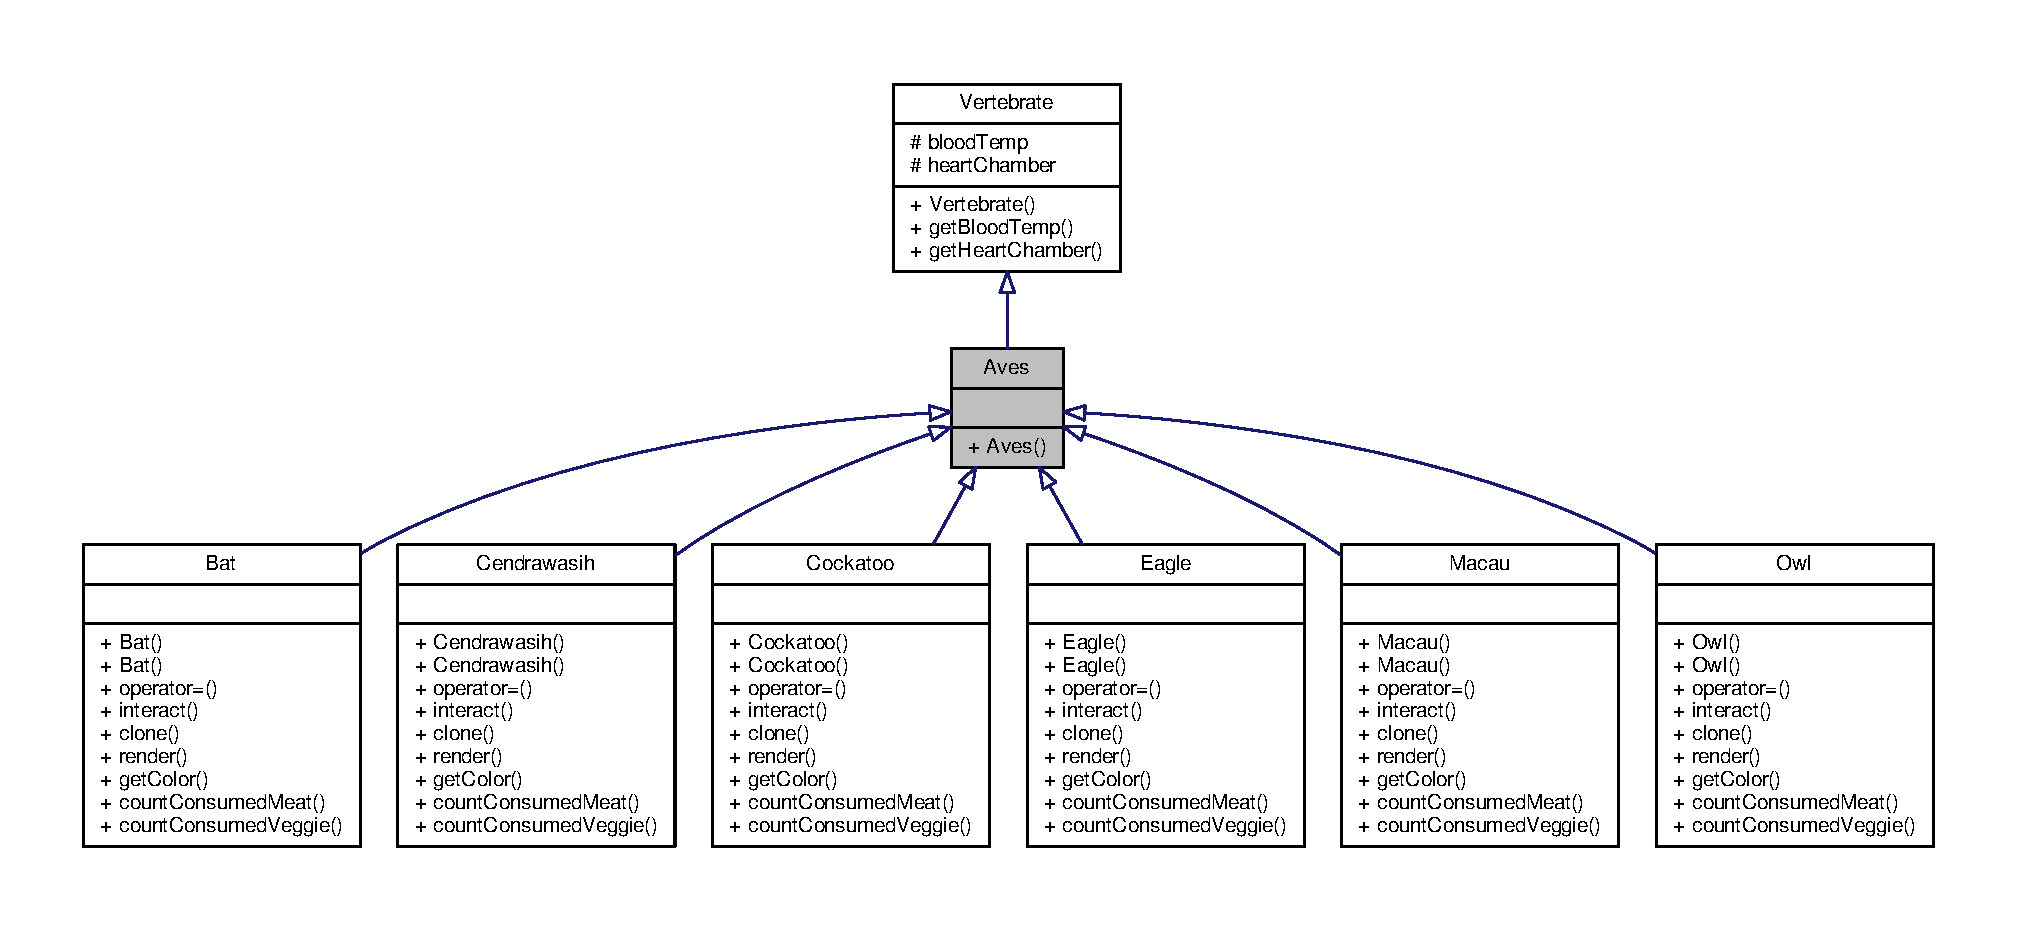
\includegraphics[width=350pt]{classAves__inherit__graph}
\end{center}
\end{figure}


Collaboration diagram for Aves\+:
\nopagebreak
\begin{figure}[H]
\begin{center}
\leavevmode
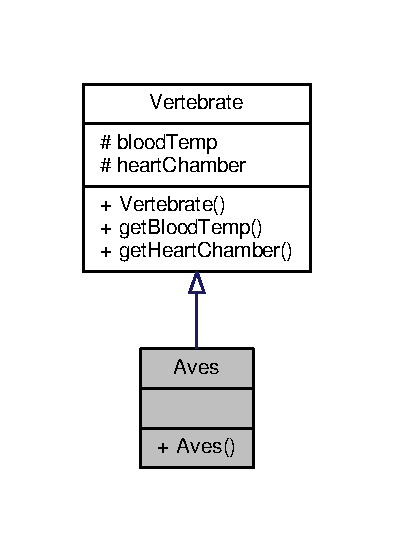
\includegraphics[width=189pt]{classAves__coll__graph}
\end{center}
\end{figure}
\subsection*{Public Member Functions}
\begin{DoxyCompactItemize}
\item 
\hyperlink{classAves_a897937de509ba03114b94b004a29f341}{Aves} ()
\begin{DoxyCompactList}\small\item\em Constructor. \end{DoxyCompactList}\end{DoxyCompactItemize}
\subsection*{Additional Inherited Members}


\subsection{Detailed Description}
Kelas taksonomi untuk burung 

\subsection{Constructor \& Destructor Documentation}
\index{Aves@{Aves}!Aves@{Aves}}
\index{Aves@{Aves}!Aves@{Aves}}
\subsubsection[{\texorpdfstring{Aves()}{Aves()}}]{\setlength{\rightskip}{0pt plus 5cm}Aves\+::\+Aves (
\begin{DoxyParamCaption}
{}
\end{DoxyParamCaption}
)}\hypertarget{classAves_a897937de509ba03114b94b004a29f341}{}\label{classAves_a897937de509ba03114b94b004a29f341}


Constructor. 



The documentation for this class was generated from the following files\+:\begin{DoxyCompactItemize}
\item 
src/renders/animals/taxonomy/\hyperlink{aves_8h}{aves.\+h}\item 
src/renders/animals/taxonomy/\hyperlink{aves_8cpp}{aves.\+cpp}\end{DoxyCompactItemize}

\hypertarget{classBat}{}\section{Bat Class Reference}
\label{classBat}\index{Bat@{Bat}}


{\ttfamily \#include $<$species.\+h$>$}



Inheritance diagram for Bat\+:
\nopagebreak
\begin{figure}[H]
\begin{center}
\leavevmode
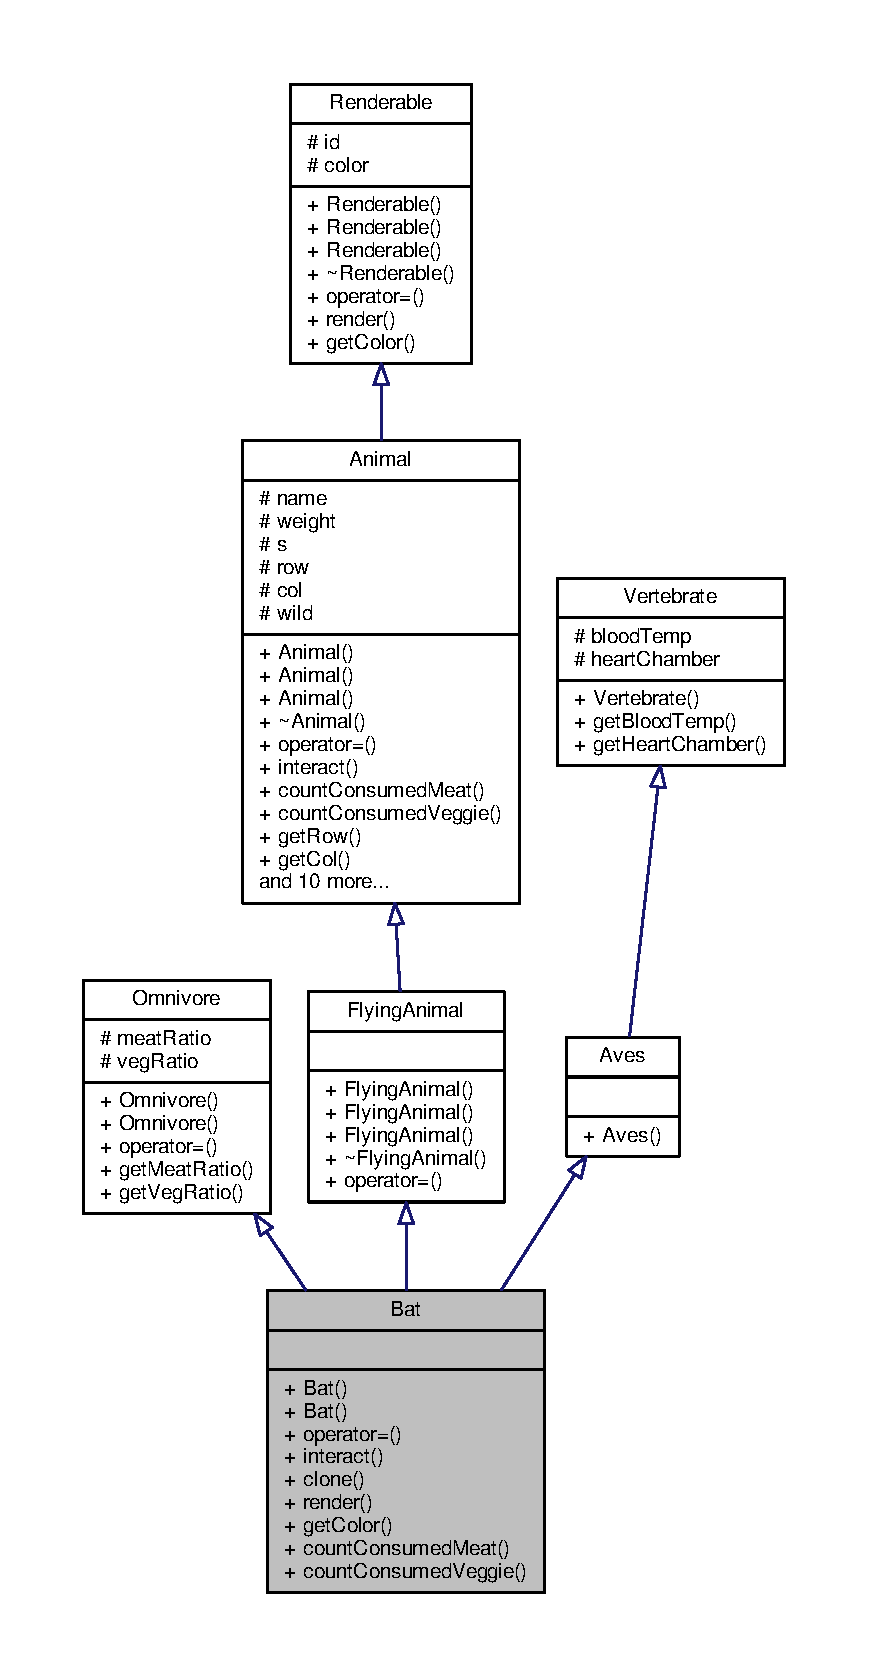
\includegraphics[height=550pt]{classBat__inherit__graph}
\end{center}
\end{figure}


Collaboration diagram for Bat\+:
\nopagebreak
\begin{figure}[H]
\begin{center}
\leavevmode
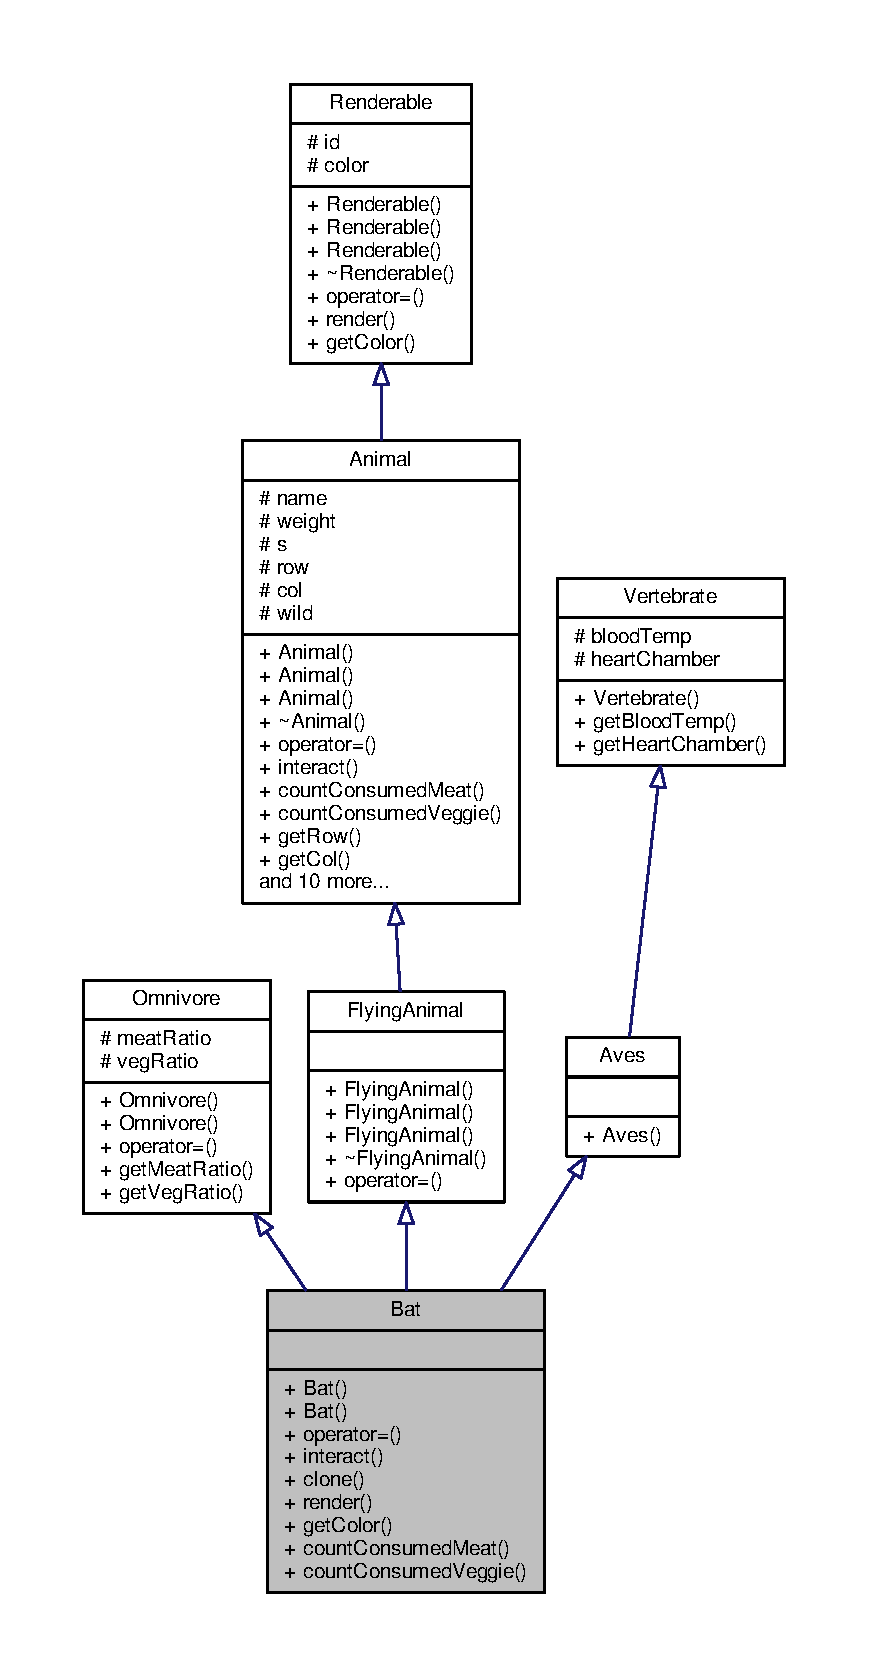
\includegraphics[height=550pt]{classBat__coll__graph}
\end{center}
\end{figure}
\subsection*{Public Member Functions}
\begin{DoxyCompactItemize}
\item 
\hyperlink{classBat_a0c530d84bcd47df69423446f42432b08}{Bat} (string \+\_\+name, double \+\_\+weight, \hyperlink{sex_8h_a2633cb393c68bb2ee8080db58fb7ba93}{Sex} \+\_\+s, int \+\_\+r, int \+\_\+c)
\begin{DoxyCompactList}\small\item\em Consructor. \end{DoxyCompactList}\item 
\hyperlink{classBat_acf84d45e08e801386877838426746725}{Bat} (const \hyperlink{classBat}{Bat} \&B)
\begin{DoxyCompactList}\small\item\em Copy Consructor. \end{DoxyCompactList}\item 
\hyperlink{classBat}{Bat} \& \hyperlink{classBat_a63fbad7b887f510a807f03950cd44af6}{operator=} (const \hyperlink{classBat}{Bat} \&B)
\begin{DoxyCompactList}\small\item\em Operator=. Melakukan assignment pada objek. \end{DoxyCompactList}\item 
virtual void \hyperlink{classBat_adf63bb33699532d83e680252c4b7021c}{interact} ()
\begin{DoxyCompactList}\small\item\em interact. Menampilkan interaksi hewan ke layar \end{DoxyCompactList}\item 
virtual \hyperlink{classBat}{Bat} $\ast$ \hyperlink{classBat_a424595b4e6c12819cc4b1a4083c756cb}{clone} () const 
\begin{DoxyCompactList}\small\item\em clone Menduplikat diri sendiri \end{DoxyCompactList}\item 
virtual char \hyperlink{classBat_a53f34e24e9247fb195c4114e53920bc3}{render} ()
\begin{DoxyCompactList}\small\item\em render Mengembalikan karakter id tiap hewan \end{DoxyCompactList}\item 
virtual \hyperlink{color_8h_ab87bacfdad76e61b9412d7124be44c1c}{Color} \hyperlink{classBat_a7f75f3924791ba21aef97876aed26475}{get\+Color} ()
\begin{DoxyCompactList}\small\item\em get\+Color Mengembalikan warna dari hewan \end{DoxyCompactList}\item 
virtual double \hyperlink{classBat_a99a15e819b635da5f3342189d02399a2}{count\+Consumed\+Meat} ()
\begin{DoxyCompactList}\small\item\em count\+Consumed\+Meat Mengembalikan jumlah daging yang dikonsumsi \end{DoxyCompactList}\item 
virtual double \hyperlink{classBat_a496ea2d647757518276d20a12d3dea44}{count\+Consumed\+Veggie} ()
\begin{DoxyCompactList}\small\item\em count\+Consumed\+Veggie Mengembalikan jumlah makanan tumbuhan yang dikonsumsi \end{DoxyCompactList}\end{DoxyCompactItemize}
\subsection*{Additional Inherited Members}


\subsection{Constructor \& Destructor Documentation}
\index{Bat@{Bat}!Bat@{Bat}}
\index{Bat@{Bat}!Bat@{Bat}}
\subsubsection[{\texorpdfstring{Bat(string \+\_\+name, double \+\_\+weight, Sex \+\_\+s, int \+\_\+r, int \+\_\+c)}{Bat(string _name, double _weight, Sex _s, int _r, int _c)}}]{\setlength{\rightskip}{0pt plus 5cm}Bat\+::\+Bat (
\begin{DoxyParamCaption}
\item[{string}]{\+\_\+name, }
\item[{double}]{\+\_\+weight, }
\item[{{\bf Sex}}]{\+\_\+s, }
\item[{int}]{\+\_\+r, }
\item[{int}]{\+\_\+c}
\end{DoxyParamCaption}
)}\hypertarget{classBat_a0c530d84bcd47df69423446f42432b08}{}\label{classBat_a0c530d84bcd47df69423446f42432b08}


Consructor. 


\begin{DoxyParams}{Parameters}
{\em \+\_\+name} & nama binatang \\
\hline
{\em \+\_\+weight} & berat \\
\hline
{\em \+\_\+s} & jenis kelamin \\
\hline
\end{DoxyParams}
\index{Bat@{Bat}!Bat@{Bat}}
\index{Bat@{Bat}!Bat@{Bat}}
\subsubsection[{\texorpdfstring{Bat(const Bat \&\+B)}{Bat(const Bat &B)}}]{\setlength{\rightskip}{0pt plus 5cm}Bat\+::\+Bat (
\begin{DoxyParamCaption}
\item[{const {\bf Bat} \&}]{B}
\end{DoxyParamCaption}
)}\hypertarget{classBat_acf84d45e08e801386877838426746725}{}\label{classBat_acf84d45e08e801386877838426746725}


Copy Consructor. 


\begin{DoxyParams}{Parameters}
{\em B} & objek yang akan disalin \\
\hline
\end{DoxyParams}


\subsection{Member Function Documentation}
\index{Bat@{Bat}!clone@{clone}}
\index{clone@{clone}!Bat@{Bat}}
\subsubsection[{\texorpdfstring{clone() const }{clone() const }}]{\setlength{\rightskip}{0pt plus 5cm}{\bf Bat} $\ast$ Bat\+::clone (
\begin{DoxyParamCaption}
{}
\end{DoxyParamCaption}
) const\hspace{0.3cm}{\ttfamily [virtual]}}\hypertarget{classBat_a424595b4e6c12819cc4b1a4083c756cb}{}\label{classBat_a424595b4e6c12819cc4b1a4083c756cb}


clone Menduplikat diri sendiri 

\begin{DoxyReturn}{Returns}
value object hasil kloning 
\end{DoxyReturn}


Implements \hyperlink{classAnimal_a1430e040ea4ff43bc453fa0ad19c308d}{Animal}.

\index{Bat@{Bat}!count\+Consumed\+Meat@{count\+Consumed\+Meat}}
\index{count\+Consumed\+Meat@{count\+Consumed\+Meat}!Bat@{Bat}}
\subsubsection[{\texorpdfstring{count\+Consumed\+Meat()}{countConsumedMeat()}}]{\setlength{\rightskip}{0pt plus 5cm}double Bat\+::count\+Consumed\+Meat (
\begin{DoxyParamCaption}
{}
\end{DoxyParamCaption}
)\hspace{0.3cm}{\ttfamily [virtual]}}\hypertarget{classBat_a99a15e819b635da5f3342189d02399a2}{}\label{classBat_a99a15e819b635da5f3342189d02399a2}


count\+Consumed\+Meat Mengembalikan jumlah daging yang dikonsumsi 

\begin{DoxyReturn}{Returns}
jumlah daging yang dikonsumsi 
\end{DoxyReturn}


Implements \hyperlink{classAnimal_a84ccc380d237650f2bf24d792627d376}{Animal}.

\index{Bat@{Bat}!count\+Consumed\+Veggie@{count\+Consumed\+Veggie}}
\index{count\+Consumed\+Veggie@{count\+Consumed\+Veggie}!Bat@{Bat}}
\subsubsection[{\texorpdfstring{count\+Consumed\+Veggie()}{countConsumedVeggie()}}]{\setlength{\rightskip}{0pt plus 5cm}double Bat\+::count\+Consumed\+Veggie (
\begin{DoxyParamCaption}
{}
\end{DoxyParamCaption}
)\hspace{0.3cm}{\ttfamily [virtual]}}\hypertarget{classBat_a496ea2d647757518276d20a12d3dea44}{}\label{classBat_a496ea2d647757518276d20a12d3dea44}


count\+Consumed\+Veggie Mengembalikan jumlah makanan tumbuhan yang dikonsumsi 

\begin{DoxyReturn}{Returns}
jumlah makanan tumbuhan yang dikonsumsi 
\end{DoxyReturn}


Implements \hyperlink{classAnimal_aaa7e4bdb7f5a10060b6dcaf09215f822}{Animal}.

\index{Bat@{Bat}!get\+Color@{get\+Color}}
\index{get\+Color@{get\+Color}!Bat@{Bat}}
\subsubsection[{\texorpdfstring{get\+Color()}{getColor()}}]{\setlength{\rightskip}{0pt plus 5cm}{\bf Color} Bat\+::get\+Color (
\begin{DoxyParamCaption}
{}
\end{DoxyParamCaption}
)\hspace{0.3cm}{\ttfamily [virtual]}}\hypertarget{classBat_a7f75f3924791ba21aef97876aed26475}{}\label{classBat_a7f75f3924791ba21aef97876aed26475}


get\+Color Mengembalikan warna dari hewan 

\begin{DoxyReturn}{Returns}
warna cetak hewan 
\end{DoxyReturn}


Implements \hyperlink{classRenderable_ab3bcc93b20929c6e92b64223344a73d5}{Renderable}.

\index{Bat@{Bat}!interact@{interact}}
\index{interact@{interact}!Bat@{Bat}}
\subsubsection[{\texorpdfstring{interact()}{interact()}}]{\setlength{\rightskip}{0pt plus 5cm}void Bat\+::interact (
\begin{DoxyParamCaption}
{}
\end{DoxyParamCaption}
)\hspace{0.3cm}{\ttfamily [virtual]}}\hypertarget{classBat_adf63bb33699532d83e680252c4b7021c}{}\label{classBat_adf63bb33699532d83e680252c4b7021c}


interact. Menampilkan interaksi hewan ke layar 



Implements \hyperlink{classAnimal_af47626b050b665e9a19525227d2b840f}{Animal}.

\index{Bat@{Bat}!operator=@{operator=}}
\index{operator=@{operator=}!Bat@{Bat}}
\subsubsection[{\texorpdfstring{operator=(const Bat \&\+B)}{operator=(const Bat &B)}}]{\setlength{\rightskip}{0pt plus 5cm}{\bf Bat} \& Bat\+::operator= (
\begin{DoxyParamCaption}
\item[{const {\bf Bat} \&}]{B}
\end{DoxyParamCaption}
)}\hypertarget{classBat_a63fbad7b887f510a807f03950cd44af6}{}\label{classBat_a63fbad7b887f510a807f03950cd44af6}


Operator=. Melakukan assignment pada objek. 


\begin{DoxyParams}{Parameters}
{\em B} & objek yang akan disalin \\
\hline
\end{DoxyParams}
\index{Bat@{Bat}!render@{render}}
\index{render@{render}!Bat@{Bat}}
\subsubsection[{\texorpdfstring{render()}{render()}}]{\setlength{\rightskip}{0pt plus 5cm}char Bat\+::render (
\begin{DoxyParamCaption}
{}
\end{DoxyParamCaption}
)\hspace{0.3cm}{\ttfamily [virtual]}}\hypertarget{classBat_a53f34e24e9247fb195c4114e53920bc3}{}\label{classBat_a53f34e24e9247fb195c4114e53920bc3}


render Mengembalikan karakter id tiap hewan 

\begin{DoxyReturn}{Returns}
karakter tiap hewan 
\end{DoxyReturn}


Implements \hyperlink{classRenderable_aafa9280e6dcfa557b3cd675221fd97b4}{Renderable}.



The documentation for this class was generated from the following files\+:\begin{DoxyCompactItemize}
\item 
src/renders/animals/\hyperlink{species_8h}{species.\+h}\item 
src/renders/animals/\hyperlink{species_8cpp}{species.\+cpp}\end{DoxyCompactItemize}

\hypertarget{classBear}{}\section{Bear Class Reference}
\label{classBear}\index{Bear@{Bear}}


{\ttfamily \#include $<$species.\+h$>$}



Inheritance diagram for Bear\+:
\nopagebreak
\begin{figure}[H]
\begin{center}
\leavevmode
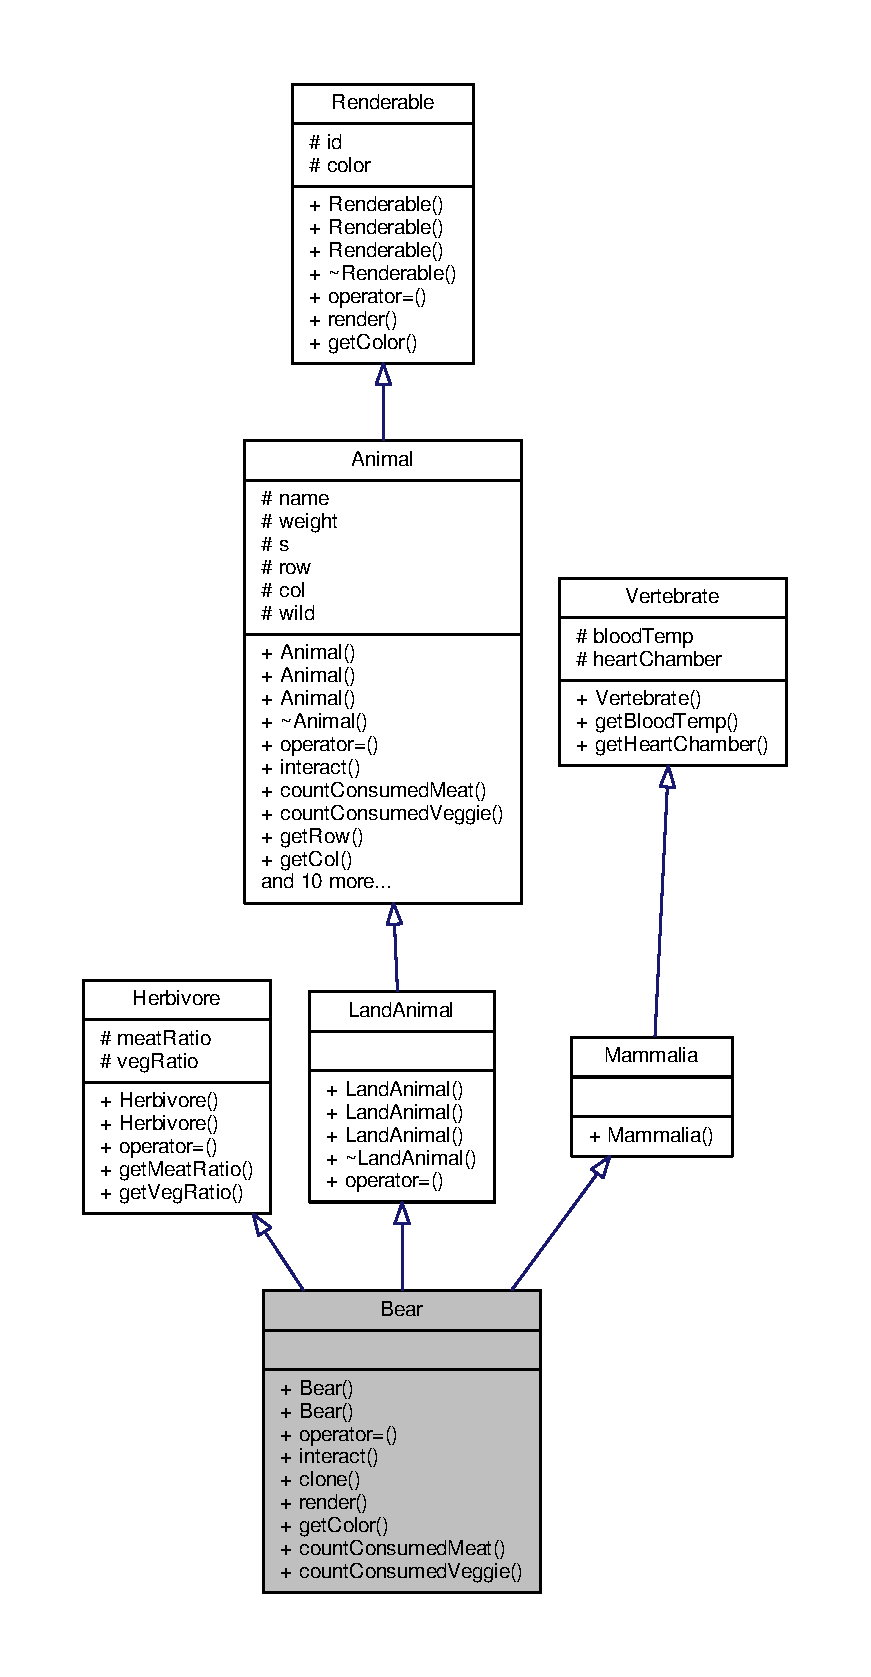
\includegraphics[height=550pt]{classBear__inherit__graph}
\end{center}
\end{figure}


Collaboration diagram for Bear\+:
\nopagebreak
\begin{figure}[H]
\begin{center}
\leavevmode
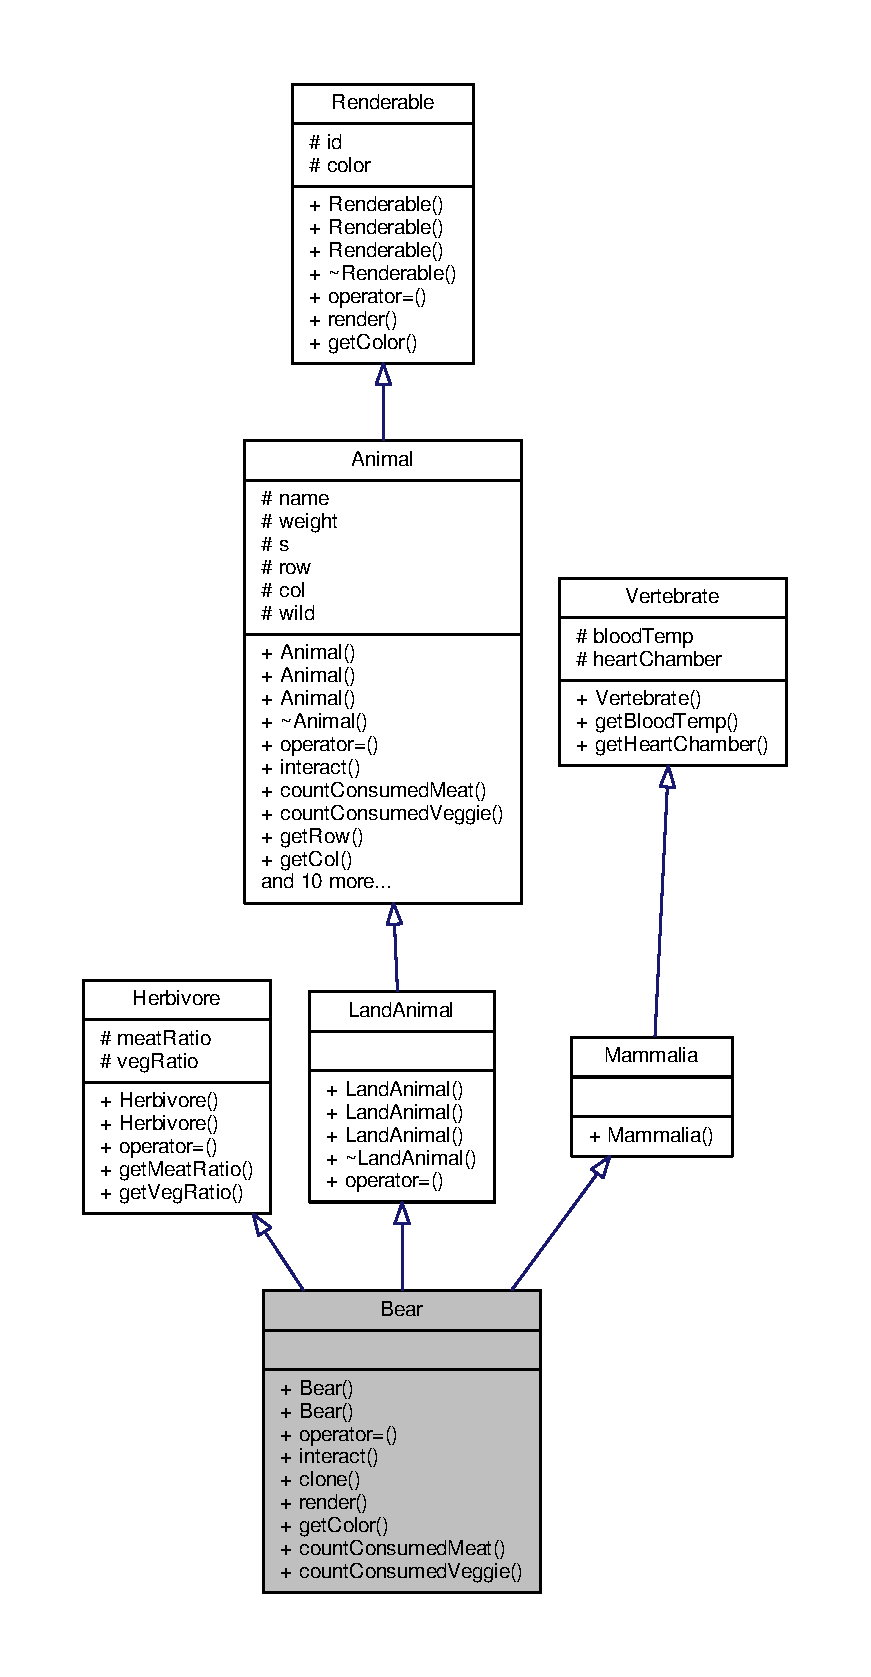
\includegraphics[height=550pt]{classBear__coll__graph}
\end{center}
\end{figure}
\subsection*{Public Member Functions}
\begin{DoxyCompactItemize}
\item 
\hyperlink{classBear_a3afafc9aa9b3dd250f6655bf9a0246f6}{Bear} (string \+\_\+name, double \+\_\+weight, \hyperlink{sex_8h_a2633cb393c68bb2ee8080db58fb7ba93}{Sex} \+\_\+s, int \+\_\+r, int \+\_\+c)
\begin{DoxyCompactList}\small\item\em Consructor. \end{DoxyCompactList}\item 
\hyperlink{classBear_a496183e4a4191809bf67634e18c83499}{Bear} (const \hyperlink{classBear}{Bear} \&B)
\begin{DoxyCompactList}\small\item\em Copy Consructor. \end{DoxyCompactList}\item 
\hyperlink{classBear}{Bear} \& \hyperlink{classBear_a6ce0207456c0c4dc02f3dced1b447405}{operator=} (const \hyperlink{classBear}{Bear} \&B)
\begin{DoxyCompactList}\small\item\em Operator=. Melakukan assignment pada objek. \end{DoxyCompactList}\item 
virtual void \hyperlink{classBear_af149829fb71fdedae09885a66964d216}{interact} ()
\begin{DoxyCompactList}\small\item\em interact. Menampilkan interaksi hewan ke layar \end{DoxyCompactList}\item 
virtual \hyperlink{classBear}{Bear} $\ast$ \hyperlink{classBear_a72baa5599585a59e57727f0f00e09e60}{clone} () const 
\begin{DoxyCompactList}\small\item\em clone Menduplikat diri sendiri \end{DoxyCompactList}\item 
virtual char \hyperlink{classBear_a2a5f7a948404e599fd37538386c384d8}{render} ()
\begin{DoxyCompactList}\small\item\em render Mengembalikan karakter id tiap hewan \end{DoxyCompactList}\item 
virtual \hyperlink{color_8h_ab87bacfdad76e61b9412d7124be44c1c}{Color} \hyperlink{classBear_ac9289a4721aa26c2f198555a9670d0d7}{get\+Color} ()
\begin{DoxyCompactList}\small\item\em get\+Color Mengembalikan warna dari hewan \end{DoxyCompactList}\item 
virtual double \hyperlink{classBear_ac4919e42fe08c1ec792abac72de24f1f}{count\+Consumed\+Meat} ()
\begin{DoxyCompactList}\small\item\em count\+Consumed\+Meat Mengembalikan jumlah daging yang dikonsumsi \end{DoxyCompactList}\item 
virtual double \hyperlink{classBear_a58587a79a0b4df2a7d9629948f339c90}{count\+Consumed\+Veggie} ()
\begin{DoxyCompactList}\small\item\em count\+Consumed\+Veggie Mengembalikan jumlah makanan tumbuhan yang dikonsumsi \end{DoxyCompactList}\end{DoxyCompactItemize}
\subsection*{Additional Inherited Members}


\subsection{Constructor \& Destructor Documentation}
\index{Bear@{Bear}!Bear@{Bear}}
\index{Bear@{Bear}!Bear@{Bear}}
\subsubsection[{\texorpdfstring{Bear(string \+\_\+name, double \+\_\+weight, Sex \+\_\+s, int \+\_\+r, int \+\_\+c)}{Bear(string _name, double _weight, Sex _s, int _r, int _c)}}]{\setlength{\rightskip}{0pt plus 5cm}Bear\+::\+Bear (
\begin{DoxyParamCaption}
\item[{string}]{\+\_\+name, }
\item[{double}]{\+\_\+weight, }
\item[{{\bf Sex}}]{\+\_\+s, }
\item[{int}]{\+\_\+r, }
\item[{int}]{\+\_\+c}
\end{DoxyParamCaption}
)}\hypertarget{classBear_a3afafc9aa9b3dd250f6655bf9a0246f6}{}\label{classBear_a3afafc9aa9b3dd250f6655bf9a0246f6}


Consructor. 


\begin{DoxyParams}{Parameters}
{\em \+\_\+name} & nama binatang \\
\hline
{\em \+\_\+weight} & berat \\
\hline
{\em \+\_\+s} & jenis kelamin \\
\hline
\end{DoxyParams}
\index{Bear@{Bear}!Bear@{Bear}}
\index{Bear@{Bear}!Bear@{Bear}}
\subsubsection[{\texorpdfstring{Bear(const Bear \&\+B)}{Bear(const Bear &B)}}]{\setlength{\rightskip}{0pt plus 5cm}Bear\+::\+Bear (
\begin{DoxyParamCaption}
\item[{const {\bf Bear} \&}]{B}
\end{DoxyParamCaption}
)}\hypertarget{classBear_a496183e4a4191809bf67634e18c83499}{}\label{classBear_a496183e4a4191809bf67634e18c83499}


Copy Consructor. 


\begin{DoxyParams}{Parameters}
{\em B} & objek yang akan disalin \\
\hline
\end{DoxyParams}


\subsection{Member Function Documentation}
\index{Bear@{Bear}!clone@{clone}}
\index{clone@{clone}!Bear@{Bear}}
\subsubsection[{\texorpdfstring{clone() const }{clone() const }}]{\setlength{\rightskip}{0pt plus 5cm}{\bf Bear} $\ast$ Bear\+::clone (
\begin{DoxyParamCaption}
{}
\end{DoxyParamCaption}
) const\hspace{0.3cm}{\ttfamily [virtual]}}\hypertarget{classBear_a72baa5599585a59e57727f0f00e09e60}{}\label{classBear_a72baa5599585a59e57727f0f00e09e60}


clone Menduplikat diri sendiri 

\begin{DoxyReturn}{Returns}
value object hasil kloning 
\end{DoxyReturn}


Implements \hyperlink{classAnimal_a1430e040ea4ff43bc453fa0ad19c308d}{Animal}.

\index{Bear@{Bear}!count\+Consumed\+Meat@{count\+Consumed\+Meat}}
\index{count\+Consumed\+Meat@{count\+Consumed\+Meat}!Bear@{Bear}}
\subsubsection[{\texorpdfstring{count\+Consumed\+Meat()}{countConsumedMeat()}}]{\setlength{\rightskip}{0pt plus 5cm}double Bear\+::count\+Consumed\+Meat (
\begin{DoxyParamCaption}
{}
\end{DoxyParamCaption}
)\hspace{0.3cm}{\ttfamily [virtual]}}\hypertarget{classBear_ac4919e42fe08c1ec792abac72de24f1f}{}\label{classBear_ac4919e42fe08c1ec792abac72de24f1f}


count\+Consumed\+Meat Mengembalikan jumlah daging yang dikonsumsi 

\begin{DoxyReturn}{Returns}
jumlah daging yang dikonsumsi 
\end{DoxyReturn}


Implements \hyperlink{classAnimal_a84ccc380d237650f2bf24d792627d376}{Animal}.

\index{Bear@{Bear}!count\+Consumed\+Veggie@{count\+Consumed\+Veggie}}
\index{count\+Consumed\+Veggie@{count\+Consumed\+Veggie}!Bear@{Bear}}
\subsubsection[{\texorpdfstring{count\+Consumed\+Veggie()}{countConsumedVeggie()}}]{\setlength{\rightskip}{0pt plus 5cm}double Bear\+::count\+Consumed\+Veggie (
\begin{DoxyParamCaption}
{}
\end{DoxyParamCaption}
)\hspace{0.3cm}{\ttfamily [virtual]}}\hypertarget{classBear_a58587a79a0b4df2a7d9629948f339c90}{}\label{classBear_a58587a79a0b4df2a7d9629948f339c90}


count\+Consumed\+Veggie Mengembalikan jumlah makanan tumbuhan yang dikonsumsi 

\begin{DoxyReturn}{Returns}
jumlah makanan tumbuhan yang dikonsumsi 
\end{DoxyReturn}


Implements \hyperlink{classAnimal_aaa7e4bdb7f5a10060b6dcaf09215f822}{Animal}.

\index{Bear@{Bear}!get\+Color@{get\+Color}}
\index{get\+Color@{get\+Color}!Bear@{Bear}}
\subsubsection[{\texorpdfstring{get\+Color()}{getColor()}}]{\setlength{\rightskip}{0pt plus 5cm}{\bf Color} Bear\+::get\+Color (
\begin{DoxyParamCaption}
{}
\end{DoxyParamCaption}
)\hspace{0.3cm}{\ttfamily [virtual]}}\hypertarget{classBear_ac9289a4721aa26c2f198555a9670d0d7}{}\label{classBear_ac9289a4721aa26c2f198555a9670d0d7}


get\+Color Mengembalikan warna dari hewan 

\begin{DoxyReturn}{Returns}
warna cetak hewan 
\end{DoxyReturn}


Implements \hyperlink{classRenderable_ab3bcc93b20929c6e92b64223344a73d5}{Renderable}.

\index{Bear@{Bear}!interact@{interact}}
\index{interact@{interact}!Bear@{Bear}}
\subsubsection[{\texorpdfstring{interact()}{interact()}}]{\setlength{\rightskip}{0pt plus 5cm}void Bear\+::interact (
\begin{DoxyParamCaption}
{}
\end{DoxyParamCaption}
)\hspace{0.3cm}{\ttfamily [virtual]}}\hypertarget{classBear_af149829fb71fdedae09885a66964d216}{}\label{classBear_af149829fb71fdedae09885a66964d216}


interact. Menampilkan interaksi hewan ke layar 



Implements \hyperlink{classAnimal_af47626b050b665e9a19525227d2b840f}{Animal}.

\index{Bear@{Bear}!operator=@{operator=}}
\index{operator=@{operator=}!Bear@{Bear}}
\subsubsection[{\texorpdfstring{operator=(const Bear \&\+B)}{operator=(const Bear &B)}}]{\setlength{\rightskip}{0pt plus 5cm}{\bf Bear} \& Bear\+::operator= (
\begin{DoxyParamCaption}
\item[{const {\bf Bear} \&}]{B}
\end{DoxyParamCaption}
)}\hypertarget{classBear_a6ce0207456c0c4dc02f3dced1b447405}{}\label{classBear_a6ce0207456c0c4dc02f3dced1b447405}


Operator=. Melakukan assignment pada objek. 


\begin{DoxyParams}{Parameters}
{\em B} & objek yang akan disalin \\
\hline
\end{DoxyParams}
\index{Bear@{Bear}!render@{render}}
\index{render@{render}!Bear@{Bear}}
\subsubsection[{\texorpdfstring{render()}{render()}}]{\setlength{\rightskip}{0pt plus 5cm}char Bear\+::render (
\begin{DoxyParamCaption}
{}
\end{DoxyParamCaption}
)\hspace{0.3cm}{\ttfamily [virtual]}}\hypertarget{classBear_a2a5f7a948404e599fd37538386c384d8}{}\label{classBear_a2a5f7a948404e599fd37538386c384d8}


render Mengembalikan karakter id tiap hewan 

\begin{DoxyReturn}{Returns}
karakter tiap hewan 
\end{DoxyReturn}


Implements \hyperlink{classRenderable_aafa9280e6dcfa557b3cd675221fd97b4}{Renderable}.



The documentation for this class was generated from the following files\+:\begin{DoxyCompactItemize}
\item 
src/renders/animals/\hyperlink{species_8h}{species.\+h}\item 
src/renders/animals/\hyperlink{species_8cpp}{species.\+cpp}\end{DoxyCompactItemize}

\hypertarget{classBlueTang}{}\section{Blue\+Tang Class Reference}
\label{classBlueTang}\index{Blue\+Tang@{Blue\+Tang}}


{\ttfamily \#include $<$species.\+h$>$}



Inheritance diagram for Blue\+Tang\+:
\nopagebreak
\begin{figure}[H]
\begin{center}
\leavevmode
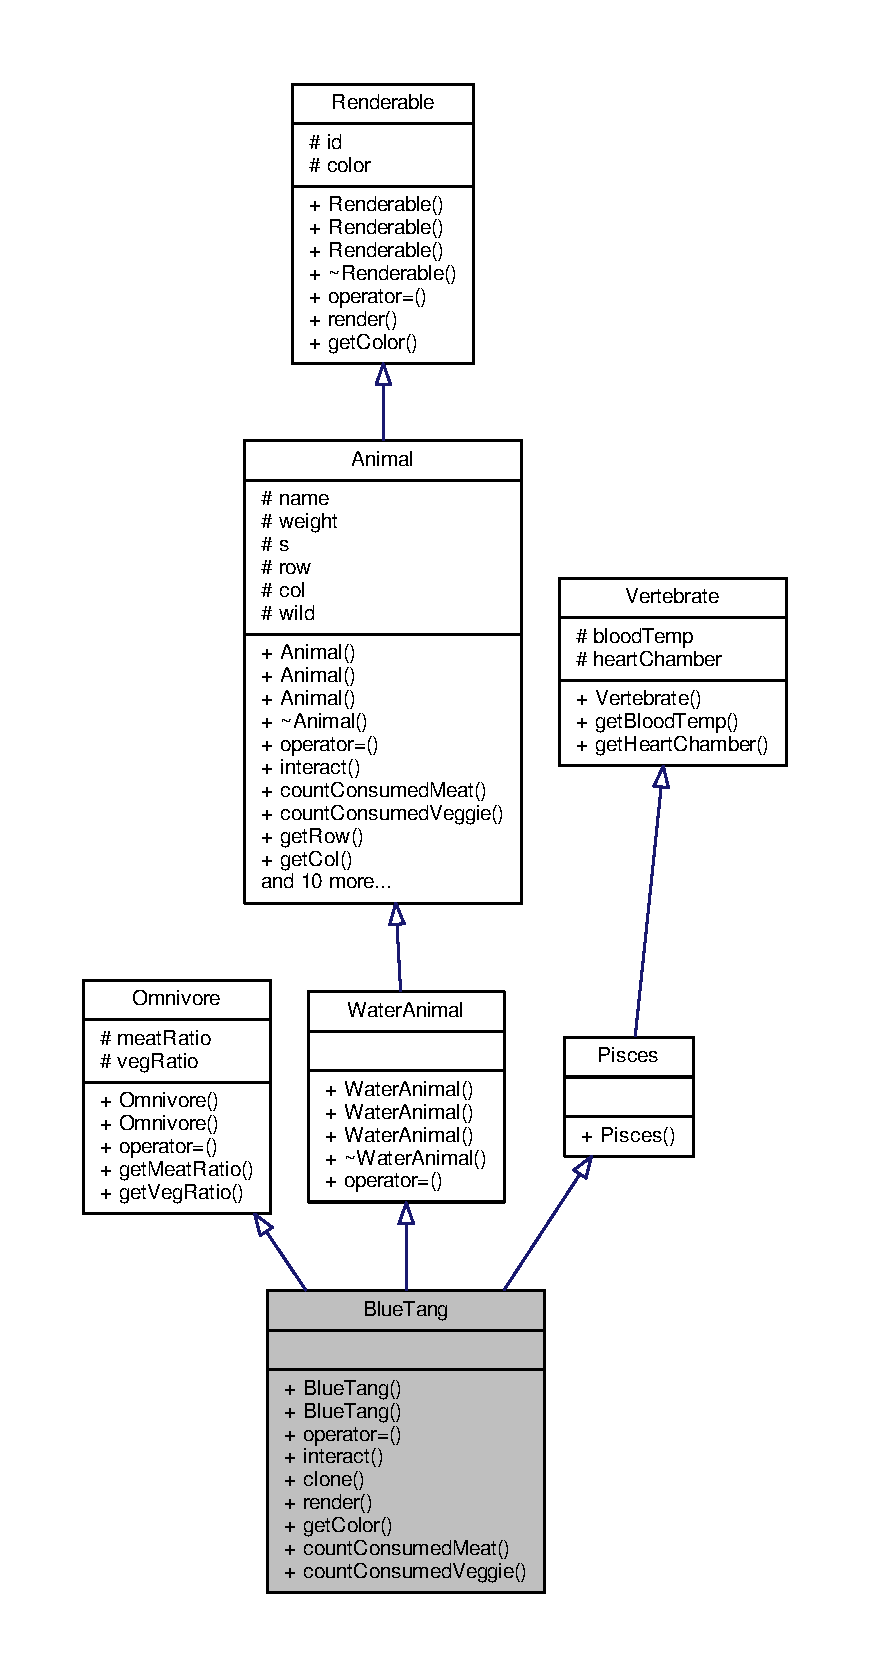
\includegraphics[height=550pt]{classBlueTang__inherit__graph}
\end{center}
\end{figure}


Collaboration diagram for Blue\+Tang\+:
\nopagebreak
\begin{figure}[H]
\begin{center}
\leavevmode
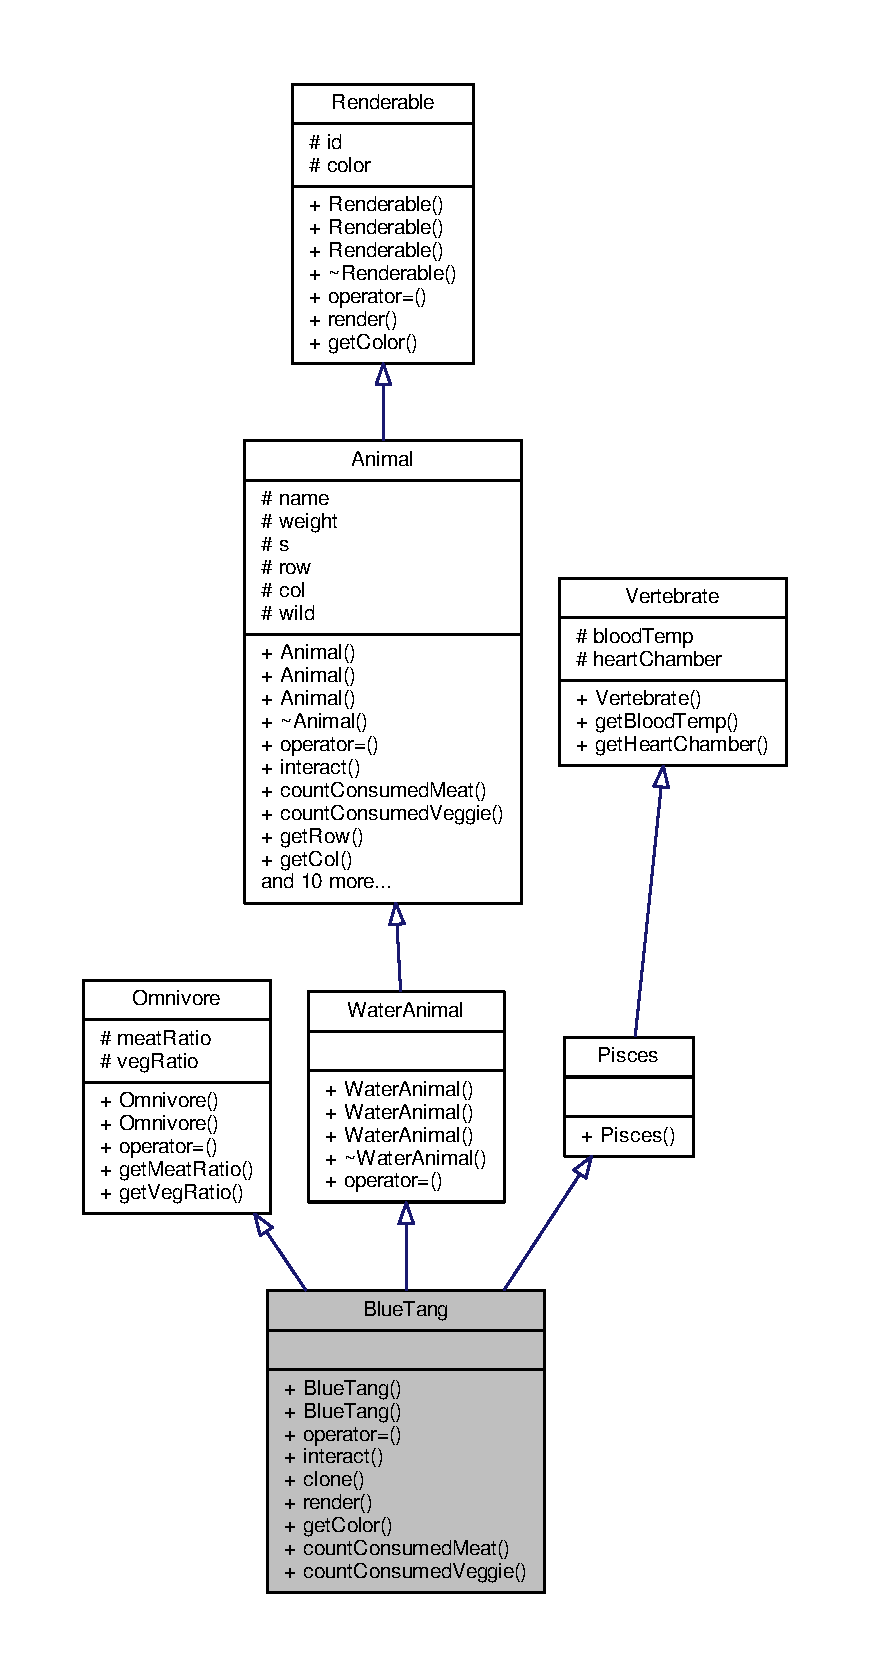
\includegraphics[height=550pt]{classBlueTang__coll__graph}
\end{center}
\end{figure}
\subsection*{Public Member Functions}
\begin{DoxyCompactItemize}
\item 
\hyperlink{classBlueTang_a13620a0a3513d70caaf1dd7a7d70389b}{Blue\+Tang} (string \+\_\+name, double \+\_\+weight, \hyperlink{sex_8h_a2633cb393c68bb2ee8080db58fb7ba93}{Sex} \+\_\+s, int \+\_\+r, int \+\_\+c)
\begin{DoxyCompactList}\small\item\em Consructor. \end{DoxyCompactList}\item 
\hyperlink{classBlueTang_adaecf8dcc061e6c4cae3b4e61ea83238}{Blue\+Tang} (const \hyperlink{classBlueTang}{Blue\+Tang} \&B)
\begin{DoxyCompactList}\small\item\em Copy Consructor. \end{DoxyCompactList}\item 
\hyperlink{classBlueTang}{Blue\+Tang} \& \hyperlink{classBlueTang_af87c19bccd039c3978c989c6ec0616fc}{operator=} (const \hyperlink{classBlueTang}{Blue\+Tang} \&B)
\begin{DoxyCompactList}\small\item\em Operator=. Melakukan assignment pada objek. \end{DoxyCompactList}\item 
virtual void \hyperlink{classBlueTang_a2cb5619f4bb30b19f54fe3c062598422}{interact} ()
\begin{DoxyCompactList}\small\item\em interact. Menampilkan interaksi hewan ke layar \end{DoxyCompactList}\item 
virtual \hyperlink{classBlueTang}{Blue\+Tang} $\ast$ \hyperlink{classBlueTang_a2b4ac8cf3cddaa66c9cc361c6cc3361b}{clone} () const 
\begin{DoxyCompactList}\small\item\em clone Menduplikat diri sendiri \end{DoxyCompactList}\item 
virtual char \hyperlink{classBlueTang_a6679edaef26a7ae9c94e8a3ca633af54}{render} ()
\begin{DoxyCompactList}\small\item\em render Mengembalikan karakter id tiap hewan \end{DoxyCompactList}\item 
virtual \hyperlink{color_8h_ab87bacfdad76e61b9412d7124be44c1c}{Color} \hyperlink{classBlueTang_a95f6a1192959bb77c51eb41c2fd0757e}{get\+Color} ()
\begin{DoxyCompactList}\small\item\em get\+Color Mengembalikan warna dari hewan \end{DoxyCompactList}\item 
virtual double \hyperlink{classBlueTang_abb9f72532beeac89a07db47010b5124b}{count\+Consumed\+Meat} ()
\begin{DoxyCompactList}\small\item\em count\+Consumed\+Meat Mengembalikan jumlah daging yang dikonsumsi \end{DoxyCompactList}\item 
virtual double \hyperlink{classBlueTang_abab5b6bae1d54d9c059076f19cd1f3af}{count\+Consumed\+Veggie} ()
\begin{DoxyCompactList}\small\item\em count\+Consumed\+Veggie Mengembalikan jumlah makanan tumbuhan yang dikonsumsi \end{DoxyCompactList}\end{DoxyCompactItemize}
\subsection*{Additional Inherited Members}


\subsection{Constructor \& Destructor Documentation}
\index{Blue\+Tang@{Blue\+Tang}!Blue\+Tang@{Blue\+Tang}}
\index{Blue\+Tang@{Blue\+Tang}!Blue\+Tang@{Blue\+Tang}}
\subsubsection[{\texorpdfstring{Blue\+Tang(string \+\_\+name, double \+\_\+weight, Sex \+\_\+s, int \+\_\+r, int \+\_\+c)}{BlueTang(string _name, double _weight, Sex _s, int _r, int _c)}}]{\setlength{\rightskip}{0pt plus 5cm}Blue\+Tang\+::\+Blue\+Tang (
\begin{DoxyParamCaption}
\item[{string}]{\+\_\+name, }
\item[{double}]{\+\_\+weight, }
\item[{{\bf Sex}}]{\+\_\+s, }
\item[{int}]{\+\_\+r, }
\item[{int}]{\+\_\+c}
\end{DoxyParamCaption}
)}\hypertarget{classBlueTang_a13620a0a3513d70caaf1dd7a7d70389b}{}\label{classBlueTang_a13620a0a3513d70caaf1dd7a7d70389b}


Consructor. 


\begin{DoxyParams}{Parameters}
{\em \+\_\+name} & nama binatang \\
\hline
{\em \+\_\+weight} & berat \\
\hline
{\em \+\_\+s} & jenis kelamin \\
\hline
\end{DoxyParams}
\index{Blue\+Tang@{Blue\+Tang}!Blue\+Tang@{Blue\+Tang}}
\index{Blue\+Tang@{Blue\+Tang}!Blue\+Tang@{Blue\+Tang}}
\subsubsection[{\texorpdfstring{Blue\+Tang(const Blue\+Tang \&\+B)}{BlueTang(const BlueTang &B)}}]{\setlength{\rightskip}{0pt plus 5cm}Blue\+Tang\+::\+Blue\+Tang (
\begin{DoxyParamCaption}
\item[{const {\bf Blue\+Tang} \&}]{B}
\end{DoxyParamCaption}
)}\hypertarget{classBlueTang_adaecf8dcc061e6c4cae3b4e61ea83238}{}\label{classBlueTang_adaecf8dcc061e6c4cae3b4e61ea83238}


Copy Consructor. 


\begin{DoxyParams}{Parameters}
{\em B} & objek yang akan disalin \\
\hline
\end{DoxyParams}


\subsection{Member Function Documentation}
\index{Blue\+Tang@{Blue\+Tang}!clone@{clone}}
\index{clone@{clone}!Blue\+Tang@{Blue\+Tang}}
\subsubsection[{\texorpdfstring{clone() const }{clone() const }}]{\setlength{\rightskip}{0pt plus 5cm}{\bf Blue\+Tang} $\ast$ Blue\+Tang\+::clone (
\begin{DoxyParamCaption}
{}
\end{DoxyParamCaption}
) const\hspace{0.3cm}{\ttfamily [virtual]}}\hypertarget{classBlueTang_a2b4ac8cf3cddaa66c9cc361c6cc3361b}{}\label{classBlueTang_a2b4ac8cf3cddaa66c9cc361c6cc3361b}


clone Menduplikat diri sendiri 

\begin{DoxyReturn}{Returns}
value object hasil kloning 
\end{DoxyReturn}


Implements \hyperlink{classAnimal_a1430e040ea4ff43bc453fa0ad19c308d}{Animal}.

\index{Blue\+Tang@{Blue\+Tang}!count\+Consumed\+Meat@{count\+Consumed\+Meat}}
\index{count\+Consumed\+Meat@{count\+Consumed\+Meat}!Blue\+Tang@{Blue\+Tang}}
\subsubsection[{\texorpdfstring{count\+Consumed\+Meat()}{countConsumedMeat()}}]{\setlength{\rightskip}{0pt plus 5cm}double Blue\+Tang\+::count\+Consumed\+Meat (
\begin{DoxyParamCaption}
{}
\end{DoxyParamCaption}
)\hspace{0.3cm}{\ttfamily [virtual]}}\hypertarget{classBlueTang_abb9f72532beeac89a07db47010b5124b}{}\label{classBlueTang_abb9f72532beeac89a07db47010b5124b}


count\+Consumed\+Meat Mengembalikan jumlah daging yang dikonsumsi 

\begin{DoxyReturn}{Returns}
jumlah daging yang dikonsumsi 
\end{DoxyReturn}


Implements \hyperlink{classAnimal_a84ccc380d237650f2bf24d792627d376}{Animal}.

\index{Blue\+Tang@{Blue\+Tang}!count\+Consumed\+Veggie@{count\+Consumed\+Veggie}}
\index{count\+Consumed\+Veggie@{count\+Consumed\+Veggie}!Blue\+Tang@{Blue\+Tang}}
\subsubsection[{\texorpdfstring{count\+Consumed\+Veggie()}{countConsumedVeggie()}}]{\setlength{\rightskip}{0pt plus 5cm}double Blue\+Tang\+::count\+Consumed\+Veggie (
\begin{DoxyParamCaption}
{}
\end{DoxyParamCaption}
)\hspace{0.3cm}{\ttfamily [virtual]}}\hypertarget{classBlueTang_abab5b6bae1d54d9c059076f19cd1f3af}{}\label{classBlueTang_abab5b6bae1d54d9c059076f19cd1f3af}


count\+Consumed\+Veggie Mengembalikan jumlah makanan tumbuhan yang dikonsumsi 

\begin{DoxyReturn}{Returns}
jumlah makanan tumbuhan yang dikonsumsi 
\end{DoxyReturn}


Implements \hyperlink{classAnimal_aaa7e4bdb7f5a10060b6dcaf09215f822}{Animal}.

\index{Blue\+Tang@{Blue\+Tang}!get\+Color@{get\+Color}}
\index{get\+Color@{get\+Color}!Blue\+Tang@{Blue\+Tang}}
\subsubsection[{\texorpdfstring{get\+Color()}{getColor()}}]{\setlength{\rightskip}{0pt plus 5cm}{\bf Color} Blue\+Tang\+::get\+Color (
\begin{DoxyParamCaption}
{}
\end{DoxyParamCaption}
)\hspace{0.3cm}{\ttfamily [virtual]}}\hypertarget{classBlueTang_a95f6a1192959bb77c51eb41c2fd0757e}{}\label{classBlueTang_a95f6a1192959bb77c51eb41c2fd0757e}


get\+Color Mengembalikan warna dari hewan 

\begin{DoxyReturn}{Returns}
warna cetak hewan 
\end{DoxyReturn}


Implements \hyperlink{classRenderable_ab3bcc93b20929c6e92b64223344a73d5}{Renderable}.

\index{Blue\+Tang@{Blue\+Tang}!interact@{interact}}
\index{interact@{interact}!Blue\+Tang@{Blue\+Tang}}
\subsubsection[{\texorpdfstring{interact()}{interact()}}]{\setlength{\rightskip}{0pt plus 5cm}void Blue\+Tang\+::interact (
\begin{DoxyParamCaption}
{}
\end{DoxyParamCaption}
)\hspace{0.3cm}{\ttfamily [virtual]}}\hypertarget{classBlueTang_a2cb5619f4bb30b19f54fe3c062598422}{}\label{classBlueTang_a2cb5619f4bb30b19f54fe3c062598422}


interact. Menampilkan interaksi hewan ke layar 



Implements \hyperlink{classAnimal_af47626b050b665e9a19525227d2b840f}{Animal}.

\index{Blue\+Tang@{Blue\+Tang}!operator=@{operator=}}
\index{operator=@{operator=}!Blue\+Tang@{Blue\+Tang}}
\subsubsection[{\texorpdfstring{operator=(const Blue\+Tang \&\+B)}{operator=(const BlueTang &B)}}]{\setlength{\rightskip}{0pt plus 5cm}{\bf Blue\+Tang} \& Blue\+Tang\+::operator= (
\begin{DoxyParamCaption}
\item[{const {\bf Blue\+Tang} \&}]{B}
\end{DoxyParamCaption}
)}\hypertarget{classBlueTang_af87c19bccd039c3978c989c6ec0616fc}{}\label{classBlueTang_af87c19bccd039c3978c989c6ec0616fc}


Operator=. Melakukan assignment pada objek. 


\begin{DoxyParams}{Parameters}
{\em B} & objek yang akan disalin \\
\hline
\end{DoxyParams}
\index{Blue\+Tang@{Blue\+Tang}!render@{render}}
\index{render@{render}!Blue\+Tang@{Blue\+Tang}}
\subsubsection[{\texorpdfstring{render()}{render()}}]{\setlength{\rightskip}{0pt plus 5cm}char Blue\+Tang\+::render (
\begin{DoxyParamCaption}
{}
\end{DoxyParamCaption}
)\hspace{0.3cm}{\ttfamily [virtual]}}\hypertarget{classBlueTang_a6679edaef26a7ae9c94e8a3ca633af54}{}\label{classBlueTang_a6679edaef26a7ae9c94e8a3ca633af54}


render Mengembalikan karakter id tiap hewan 

\begin{DoxyReturn}{Returns}
karakter tiap hewan 
\end{DoxyReturn}


Implements \hyperlink{classRenderable_aafa9280e6dcfa557b3cd675221fd97b4}{Renderable}.



The documentation for this class was generated from the following files\+:\begin{DoxyCompactItemize}
\item 
src/renders/animals/\hyperlink{species_8h}{species.\+h}\item 
src/renders/animals/\hyperlink{species_8cpp}{species.\+cpp}\end{DoxyCompactItemize}

\hypertarget{classCage}{}\section{Cage Class Reference}
\label{classCage}\index{Cage@{Cage}}


{\ttfamily \#include $<$cage.\+h$>$}



Inheritance diagram for Cage\+:
\nopagebreak
\begin{figure}[H]
\begin{center}
\leavevmode
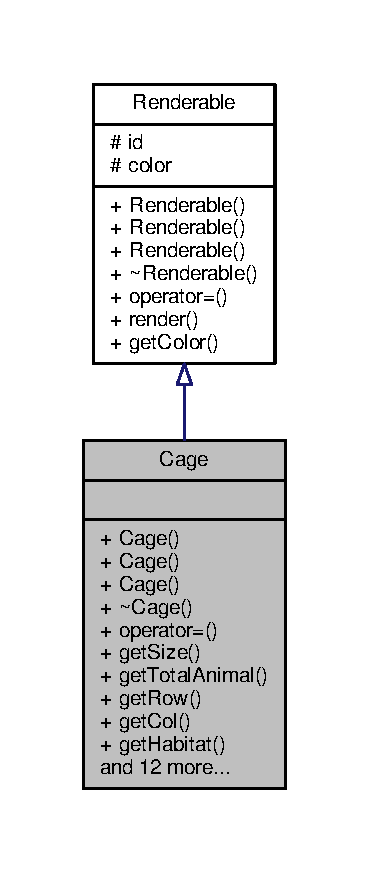
\includegraphics[width=177pt]{classCage__inherit__graph}
\end{center}
\end{figure}


Collaboration diagram for Cage\+:
\nopagebreak
\begin{figure}[H]
\begin{center}
\leavevmode
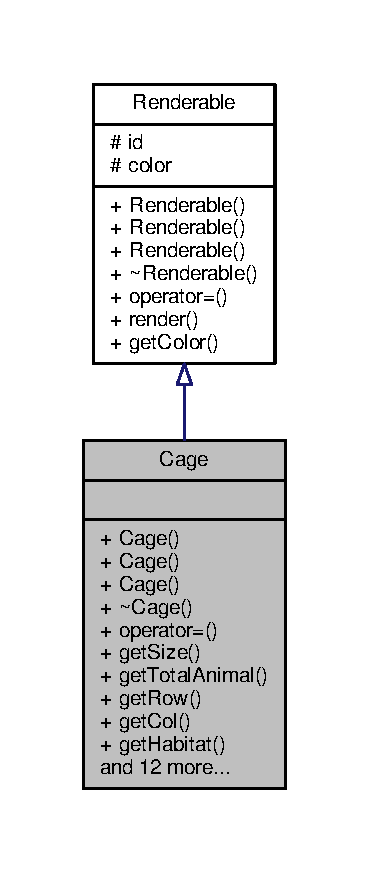
\includegraphics[width=177pt]{classCage__coll__graph}
\end{center}
\end{figure}
\subsection*{Public Member Functions}
\begin{DoxyCompactItemize}
\item 
\hyperlink{classCage_ac03246dd263ee9fe6f37336317e62b69}{Cage} ()
\begin{DoxyCompactList}\small\item\em Constructor membuat cage kosong. \end{DoxyCompactList}\item 
\hyperlink{classCage_a8cd728b1eb23303888a153230f96490e}{Cage} (int s)
\begin{DoxyCompactList}\small\item\em Constructor dengan parameter. \end{DoxyCompactList}\item 
\hyperlink{classCage_ae91dd77b358348f937432b6c48b17ea1}{Cage} (const \hyperlink{classCage}{Cage} \&C)
\begin{DoxyCompactList}\small\item\em Copy Constructor. \end{DoxyCompactList}\item 
virtual \hyperlink{classCage_a657259499dfc23c63fc65aeaf8abbb17}{$\sim$\+Cage} ()
\begin{DoxyCompactList}\small\item\em Destructor. \end{DoxyCompactList}\item 
\hyperlink{classCage}{Cage} \& \hyperlink{classCage_affbe712dc15637fc8f311aa175b66e6d}{operator=} (const \hyperlink{classCage}{Cage} \&C)
\begin{DoxyCompactList}\small\item\em Operator=. Menjamin bukan bitwise copy. \end{DoxyCompactList}\item 
int \hyperlink{classCage_a20b2c76f39601430f67645cac4c5888f}{get\+Size} () const 
\begin{DoxyCompactList}\small\item\em Get\+Size. Mengembalikan ukuran \hyperlink{classCage}{Cage}. \end{DoxyCompactList}\item 
int \hyperlink{classCage_a287b1e3bec3e49102141e5848365c9d9}{get\+Total\+Animal} () const 
\begin{DoxyCompactList}\small\item\em Get\+Total\+Animal. Mengembalikan banyaknya binatang dalam satu cage. \end{DoxyCompactList}\item 
int $\ast$ \hyperlink{classCage_a772fc432329f4f31dec41e6b7420b738}{get\+Row} () const 
\begin{DoxyCompactList}\small\item\em Get\+Row. Mengembalikan posisi baris. \end{DoxyCompactList}\item 
int $\ast$ \hyperlink{classCage_a89adfc6b5d08120c6be34753cc340666}{get\+Col} () const 
\begin{DoxyCompactList}\small\item\em Get\+Col. Mengembalikan posisi kolom. \end{DoxyCompactList}\item 
char \hyperlink{classCage_a9840593873ce0d8e5da91045883f4bfc}{get\+Habitat} () const 
\begin{DoxyCompactList}\small\item\em get\+Habitat. Mengembalikan nilai habitat kandang. \end{DoxyCompactList}\item 
\hyperlink{classAnimal}{Animal} $\ast$ \hyperlink{classCage_a4671c9ad04e70ca66517fde53267954f}{get\+Animal} (int x) const 
\begin{DoxyCompactList}\small\item\em get\+Animal. Mengembalikan pointer ke hewan dari array pada indeks x. \end{DoxyCompactList}\item 
bool \hyperlink{classCage_a6e4f2417918ef61eee36cdf27a807a8d}{is\+Full} () const 
\begin{DoxyCompactList}\small\item\em is\+Full. Mengembalikan true jika 30\% cage berisi binatang \end{DoxyCompactList}\item 
void \hyperlink{classCage_a2123b8cbc7177526b9da8a098bc19afd}{Add\+Animal} (const \hyperlink{classAnimal}{Animal} $\ast$A)
\begin{DoxyCompactList}\small\item\em Add\+Animal. Menambahkan binatang ke dalam cage. \end{DoxyCompactList}\item 
void \hyperlink{classCage_a449f19d08289f70a140955a99769ae4a}{Move} ()
\begin{DoxyCompactList}\small\item\em Move. Menggerakan semua hewan ke posisi yang berbeda dari semula bila memungkinkan. \end{DoxyCompactList}\item 
double \hyperlink{classCage_a4acb30ffa8df06db080019ecf35824a2}{count\+Consumed\+Meat} ()
\begin{DoxyCompactList}\small\item\em count\+Consumed\+Meat. Menghitung jumlah makanan daging \end{DoxyCompactList}\item 
double \hyperlink{classCage_a57c2ea58b99c5990bdf9f712841c0334}{count\+Consumed\+Veggie} ()
\begin{DoxyCompactList}\small\item\em count\+Consumed\+Veggie. Menghitung jumlah makanan sayuran \end{DoxyCompactList}\item 
char \hyperlink{classCage_aab864d541ada79ac83619b139bef5507}{render} ()
\begin{DoxyCompactList}\small\item\em render. Mengembalikan karakter yang merepresentasikan cage sesuai habitatnya \end{DoxyCompactList}\item 
\hyperlink{color_8h_ab87bacfdad76e61b9412d7124be44c1c}{Color} \hyperlink{classCage_a95f3b253744419722bf5ccbda06faf62}{get\+Color} ()
\begin{DoxyCompactList}\small\item\em get\+Color. Mengembalikan warna yang merepresentasikan cage \end{DoxyCompactList}\item 
void \hyperlink{classCage_ab879106b3284eef081bb14096db7c9aa}{set\+Habitat} (char c)
\begin{DoxyCompactList}\small\item\em Setter \hyperlink{classHabitat}{Habitat}. Menginisialisasi habitat cage dengan c I.\+S. kandang belum dihuni animal. \end{DoxyCompactList}\item 
bool \hyperlink{classCage_a128e52e1da32a761113545f84a82c163}{Search\+Pos} (int r, int c)
\begin{DoxyCompactList}\small\item\em Search\+Pos. Mengecek apakah ada pasangan r dan c pada cage. \end{DoxyCompactList}\item 
bool \hyperlink{classCage_a75988c8f55ed212612c012ba94b8815e}{Search\+Animal} (int r, int c)
\begin{DoxyCompactList}\small\item\em Search\+Animal. Mengecek apakah ada animal yang berposisi r dan c pada cage. \end{DoxyCompactList}\item 
void \hyperlink{classCage_a10346b885c28f4d8cc0d3d4e5a0ca5c9}{print\+Interact} ()
\begin{DoxyCompactList}\small\item\em Mencetak interaksi. Mencetak interaksi pengunjung terhadap suatu kandang. Prosesnya dengan mencetak semua interaksi dengan hewan yang ada di kandang. \end{DoxyCompactList}\end{DoxyCompactItemize}
\subsection*{Friends}
\begin{DoxyCompactItemize}
\item 
istream \& \hyperlink{classCage_aafb3403e12ffcf026832b69fbf3ed778}{operator$>$$>$} (istream \&in, \hyperlink{classCage}{Cage} \&C)
\begin{DoxyCompactList}\small\item\em Operator$>$$>$. Menambahkan binatang ke dalam cage. \end{DoxyCompactList}\end{DoxyCompactItemize}
\subsection*{Additional Inherited Members}


\subsection{Detailed Description}
Kelas yang merepresentasikan kandang yang terdiri dari habitat kandang, posisi-\/posisi yang dicakup kandang, dan hewan yang tinggal di kandang. 

\subsection{Constructor \& Destructor Documentation}
\index{Cage@{Cage}!Cage@{Cage}}
\index{Cage@{Cage}!Cage@{Cage}}
\subsubsection[{\texorpdfstring{Cage()}{Cage()}}]{\setlength{\rightskip}{0pt plus 5cm}Cage\+::\+Cage (
\begin{DoxyParamCaption}
{}
\end{DoxyParamCaption}
)}\hypertarget{classCage_ac03246dd263ee9fe6f37336317e62b69}{}\label{classCage_ac03246dd263ee9fe6f37336317e62b69}


Constructor membuat cage kosong. 

\index{Cage@{Cage}!Cage@{Cage}}
\index{Cage@{Cage}!Cage@{Cage}}
\subsubsection[{\texorpdfstring{Cage(int s)}{Cage(int s)}}]{\setlength{\rightskip}{0pt plus 5cm}Cage\+::\+Cage (
\begin{DoxyParamCaption}
\item[{int}]{s}
\end{DoxyParamCaption}
)}\hypertarget{classCage_a8cd728b1eb23303888a153230f96490e}{}\label{classCage_a8cd728b1eb23303888a153230f96490e}


Constructor dengan parameter. 


\begin{DoxyParams}{Parameters}
{\em s} & ukuran cage \\
\hline
\end{DoxyParams}
\index{Cage@{Cage}!Cage@{Cage}}
\index{Cage@{Cage}!Cage@{Cage}}
\subsubsection[{\texorpdfstring{Cage(const Cage \&\+C)}{Cage(const Cage &C)}}]{\setlength{\rightskip}{0pt plus 5cm}Cage\+::\+Cage (
\begin{DoxyParamCaption}
\item[{const {\bf Cage} \&}]{C}
\end{DoxyParamCaption}
)}\hypertarget{classCage_ae91dd77b358348f937432b6c48b17ea1}{}\label{classCage_ae91dd77b358348f937432b6c48b17ea1}


Copy Constructor. 


\begin{DoxyParams}{Parameters}
{\em \hyperlink{classCage}{Cage}} & C yang diacu cctor \\
\hline
\end{DoxyParams}
\index{Cage@{Cage}!````~Cage@{$\sim$\+Cage}}
\index{````~Cage@{$\sim$\+Cage}!Cage@{Cage}}
\subsubsection[{\texorpdfstring{$\sim$\+Cage()}{~Cage()}}]{\setlength{\rightskip}{0pt plus 5cm}Cage\+::$\sim$\+Cage (
\begin{DoxyParamCaption}
{}
\end{DoxyParamCaption}
)\hspace{0.3cm}{\ttfamily [virtual]}}\hypertarget{classCage_a657259499dfc23c63fc65aeaf8abbb17}{}\label{classCage_a657259499dfc23c63fc65aeaf8abbb17}


Destructor. 



\subsection{Member Function Documentation}
\index{Cage@{Cage}!Add\+Animal@{Add\+Animal}}
\index{Add\+Animal@{Add\+Animal}!Cage@{Cage}}
\subsubsection[{\texorpdfstring{Add\+Animal(const Animal $\ast$\+A)}{AddAnimal(const Animal *A)}}]{\setlength{\rightskip}{0pt plus 5cm}void Cage\+::\+Add\+Animal (
\begin{DoxyParamCaption}
\item[{const {\bf Animal} $\ast$}]{A}
\end{DoxyParamCaption}
)}\hypertarget{classCage_a2123b8cbc7177526b9da8a098bc19afd}{}\label{classCage_a2123b8cbc7177526b9da8a098bc19afd}


Add\+Animal. Menambahkan binatang ke dalam cage. 


\begin{DoxyParams}{Parameters}
{\em pointer} & A animal \\
\hline
\end{DoxyParams}
\index{Cage@{Cage}!count\+Consumed\+Meat@{count\+Consumed\+Meat}}
\index{count\+Consumed\+Meat@{count\+Consumed\+Meat}!Cage@{Cage}}
\subsubsection[{\texorpdfstring{count\+Consumed\+Meat()}{countConsumedMeat()}}]{\setlength{\rightskip}{0pt plus 5cm}double Cage\+::count\+Consumed\+Meat (
\begin{DoxyParamCaption}
{}
\end{DoxyParamCaption}
)}\hypertarget{classCage_a4acb30ffa8df06db080019ecf35824a2}{}\label{classCage_a4acb30ffa8df06db080019ecf35824a2}


count\+Consumed\+Meat. Menghitung jumlah makanan daging 

\begin{DoxyReturn}{Returns}
jumlah daging 
\end{DoxyReturn}
\index{Cage@{Cage}!count\+Consumed\+Veggie@{count\+Consumed\+Veggie}}
\index{count\+Consumed\+Veggie@{count\+Consumed\+Veggie}!Cage@{Cage}}
\subsubsection[{\texorpdfstring{count\+Consumed\+Veggie()}{countConsumedVeggie()}}]{\setlength{\rightskip}{0pt plus 5cm}double Cage\+::count\+Consumed\+Veggie (
\begin{DoxyParamCaption}
{}
\end{DoxyParamCaption}
)}\hypertarget{classCage_a57c2ea58b99c5990bdf9f712841c0334}{}\label{classCage_a57c2ea58b99c5990bdf9f712841c0334}


count\+Consumed\+Veggie. Menghitung jumlah makanan sayuran 

\begin{DoxyReturn}{Returns}
jumlah sayuran 
\end{DoxyReturn}
\index{Cage@{Cage}!get\+Animal@{get\+Animal}}
\index{get\+Animal@{get\+Animal}!Cage@{Cage}}
\subsubsection[{\texorpdfstring{get\+Animal(int x) const }{getAnimal(int x) const }}]{\setlength{\rightskip}{0pt plus 5cm}{\bf Animal} $\ast$ Cage\+::get\+Animal (
\begin{DoxyParamCaption}
\item[{int}]{x}
\end{DoxyParamCaption}
) const}\hypertarget{classCage_a4671c9ad04e70ca66517fde53267954f}{}\label{classCage_a4671c9ad04e70ca66517fde53267954f}


get\+Animal. Mengembalikan pointer ke hewan dari array pada indeks x. 


\begin{DoxyParams}{Parameters}
{\em x} & indeks pada array hewan \\
\hline
\end{DoxyParams}
\begin{DoxyReturn}{Returns}
pointer to \hyperlink{classAnimal}{Animal} 
\end{DoxyReturn}
\index{Cage@{Cage}!get\+Col@{get\+Col}}
\index{get\+Col@{get\+Col}!Cage@{Cage}}
\subsubsection[{\texorpdfstring{get\+Col() const }{getCol() const }}]{\setlength{\rightskip}{0pt plus 5cm}int $\ast$ Cage\+::get\+Col (
\begin{DoxyParamCaption}
{}
\end{DoxyParamCaption}
) const}\hypertarget{classCage_a89adfc6b5d08120c6be34753cc340666}{}\label{classCage_a89adfc6b5d08120c6be34753cc340666}


Get\+Col. Mengembalikan posisi kolom. 

\begin{DoxyReturn}{Returns}
posisi kolom 
\end{DoxyReturn}
\index{Cage@{Cage}!get\+Color@{get\+Color}}
\index{get\+Color@{get\+Color}!Cage@{Cage}}
\subsubsection[{\texorpdfstring{get\+Color()}{getColor()}}]{\setlength{\rightskip}{0pt plus 5cm}{\bf Color} Cage\+::get\+Color (
\begin{DoxyParamCaption}
{}
\end{DoxyParamCaption}
)\hspace{0.3cm}{\ttfamily [virtual]}}\hypertarget{classCage_a95f3b253744419722bf5ccbda06faf62}{}\label{classCage_a95f3b253744419722bf5ccbda06faf62}


get\+Color. Mengembalikan warna yang merepresentasikan cage 

\begin{DoxyReturn}{Returns}
color warna cage 
\end{DoxyReturn}


Implements \hyperlink{classRenderable_ab3bcc93b20929c6e92b64223344a73d5}{Renderable}.

\index{Cage@{Cage}!get\+Habitat@{get\+Habitat}}
\index{get\+Habitat@{get\+Habitat}!Cage@{Cage}}
\subsubsection[{\texorpdfstring{get\+Habitat() const }{getHabitat() const }}]{\setlength{\rightskip}{0pt plus 5cm}char Cage\+::get\+Habitat (
\begin{DoxyParamCaption}
{}
\end{DoxyParamCaption}
) const}\hypertarget{classCage_a9840593873ce0d8e5da91045883f4bfc}{}\label{classCage_a9840593873ce0d8e5da91045883f4bfc}


get\+Habitat. Mengembalikan nilai habitat kandang. 

\begin{DoxyReturn}{Returns}
karakter habitat 
\end{DoxyReturn}
\index{Cage@{Cage}!get\+Row@{get\+Row}}
\index{get\+Row@{get\+Row}!Cage@{Cage}}
\subsubsection[{\texorpdfstring{get\+Row() const }{getRow() const }}]{\setlength{\rightskip}{0pt plus 5cm}int $\ast$ Cage\+::get\+Row (
\begin{DoxyParamCaption}
{}
\end{DoxyParamCaption}
) const}\hypertarget{classCage_a772fc432329f4f31dec41e6b7420b738}{}\label{classCage_a772fc432329f4f31dec41e6b7420b738}


Get\+Row. Mengembalikan posisi baris. 

\begin{DoxyReturn}{Returns}
posisi baris 
\end{DoxyReturn}
\index{Cage@{Cage}!get\+Size@{get\+Size}}
\index{get\+Size@{get\+Size}!Cage@{Cage}}
\subsubsection[{\texorpdfstring{get\+Size() const }{getSize() const }}]{\setlength{\rightskip}{0pt plus 5cm}int Cage\+::get\+Size (
\begin{DoxyParamCaption}
{}
\end{DoxyParamCaption}
) const}\hypertarget{classCage_a20b2c76f39601430f67645cac4c5888f}{}\label{classCage_a20b2c76f39601430f67645cac4c5888f}


Get\+Size. Mengembalikan ukuran \hyperlink{classCage}{Cage}. 

\begin{DoxyReturn}{Returns}
integer ukuran cage 
\end{DoxyReturn}
\index{Cage@{Cage}!get\+Total\+Animal@{get\+Total\+Animal}}
\index{get\+Total\+Animal@{get\+Total\+Animal}!Cage@{Cage}}
\subsubsection[{\texorpdfstring{get\+Total\+Animal() const }{getTotalAnimal() const }}]{\setlength{\rightskip}{0pt plus 5cm}int Cage\+::get\+Total\+Animal (
\begin{DoxyParamCaption}
{}
\end{DoxyParamCaption}
) const}\hypertarget{classCage_a287b1e3bec3e49102141e5848365c9d9}{}\label{classCage_a287b1e3bec3e49102141e5848365c9d9}


Get\+Total\+Animal. Mengembalikan banyaknya binatang dalam satu cage. 

\begin{DoxyReturn}{Returns}
integer banyaknya binatang 
\end{DoxyReturn}
\index{Cage@{Cage}!is\+Full@{is\+Full}}
\index{is\+Full@{is\+Full}!Cage@{Cage}}
\subsubsection[{\texorpdfstring{is\+Full() const }{isFull() const }}]{\setlength{\rightskip}{0pt plus 5cm}bool Cage\+::is\+Full (
\begin{DoxyParamCaption}
{}
\end{DoxyParamCaption}
) const}\hypertarget{classCage_a6e4f2417918ef61eee36cdf27a807a8d}{}\label{classCage_a6e4f2417918ef61eee36cdf27a807a8d}


is\+Full. Mengembalikan true jika 30\% cage berisi binatang 

\begin{DoxyReturn}{Returns}
mengembalikan true/false 
\end{DoxyReturn}
\index{Cage@{Cage}!Move@{Move}}
\index{Move@{Move}!Cage@{Cage}}
\subsubsection[{\texorpdfstring{Move()}{Move()}}]{\setlength{\rightskip}{0pt plus 5cm}void Cage\+::\+Move (
\begin{DoxyParamCaption}
{}
\end{DoxyParamCaption}
)}\hypertarget{classCage_a449f19d08289f70a140955a99769ae4a}{}\label{classCage_a449f19d08289f70a140955a99769ae4a}


Move. Menggerakan semua hewan ke posisi yang berbeda dari semula bila memungkinkan. 

\index{Cage@{Cage}!operator=@{operator=}}
\index{operator=@{operator=}!Cage@{Cage}}
\subsubsection[{\texorpdfstring{operator=(const Cage \&\+C)}{operator=(const Cage &C)}}]{\setlength{\rightskip}{0pt plus 5cm}{\bf Cage} \& Cage\+::operator= (
\begin{DoxyParamCaption}
\item[{const {\bf Cage} \&}]{C}
\end{DoxyParamCaption}
)}\hypertarget{classCage_affbe712dc15637fc8f311aa175b66e6d}{}\label{classCage_affbe712dc15637fc8f311aa175b66e6d}


Operator=. Menjamin bukan bitwise copy. 


\begin{DoxyParams}{Parameters}
{\em \hyperlink{classCage}{Cage}} & C berisi data untuk diassign \\
\hline
\end{DoxyParams}
\index{Cage@{Cage}!print\+Interact@{print\+Interact}}
\index{print\+Interact@{print\+Interact}!Cage@{Cage}}
\subsubsection[{\texorpdfstring{print\+Interact()}{printInteract()}}]{\setlength{\rightskip}{0pt plus 5cm}void Cage\+::print\+Interact (
\begin{DoxyParamCaption}
{}
\end{DoxyParamCaption}
)}\hypertarget{classCage_a10346b885c28f4d8cc0d3d4e5a0ca5c9}{}\label{classCage_a10346b885c28f4d8cc0d3d4e5a0ca5c9}


Mencetak interaksi. Mencetak interaksi pengunjung terhadap suatu kandang. Prosesnya dengan mencetak semua interaksi dengan hewan yang ada di kandang. 

\index{Cage@{Cage}!render@{render}}
\index{render@{render}!Cage@{Cage}}
\subsubsection[{\texorpdfstring{render()}{render()}}]{\setlength{\rightskip}{0pt plus 5cm}char Cage\+::render (
\begin{DoxyParamCaption}
{}
\end{DoxyParamCaption}
)\hspace{0.3cm}{\ttfamily [virtual]}}\hypertarget{classCage_aab864d541ada79ac83619b139bef5507}{}\label{classCage_aab864d541ada79ac83619b139bef5507}


render. Mengembalikan karakter yang merepresentasikan cage sesuai habitatnya 

\begin{DoxyReturn}{Returns}
karakter representasi cage 
\end{DoxyReturn}


Implements \hyperlink{classRenderable_aafa9280e6dcfa557b3cd675221fd97b4}{Renderable}.

\index{Cage@{Cage}!Search\+Animal@{Search\+Animal}}
\index{Search\+Animal@{Search\+Animal}!Cage@{Cage}}
\subsubsection[{\texorpdfstring{Search\+Animal(int r, int c)}{SearchAnimal(int r, int c)}}]{\setlength{\rightskip}{0pt plus 5cm}bool Cage\+::\+Search\+Animal (
\begin{DoxyParamCaption}
\item[{int}]{r, }
\item[{int}]{c}
\end{DoxyParamCaption}
)}\hypertarget{classCage_a75988c8f55ed212612c012ba94b8815e}{}\label{classCage_a75988c8f55ed212612c012ba94b8815e}


Search\+Animal. Mengecek apakah ada animal yang berposisi r dan c pada cage. 

\begin{DoxyReturn}{Returns}
true jika ada,false jika tidak ada 
\end{DoxyReturn}
\index{Cage@{Cage}!Search\+Pos@{Search\+Pos}}
\index{Search\+Pos@{Search\+Pos}!Cage@{Cage}}
\subsubsection[{\texorpdfstring{Search\+Pos(int r, int c)}{SearchPos(int r, int c)}}]{\setlength{\rightskip}{0pt plus 5cm}bool Cage\+::\+Search\+Pos (
\begin{DoxyParamCaption}
\item[{int}]{r, }
\item[{int}]{c}
\end{DoxyParamCaption}
)}\hypertarget{classCage_a128e52e1da32a761113545f84a82c163}{}\label{classCage_a128e52e1da32a761113545f84a82c163}


Search\+Pos. Mengecek apakah ada pasangan r dan c pada cage. 

\begin{DoxyReturn}{Returns}
true jika ada,false jika tidak ada 
\end{DoxyReturn}
\index{Cage@{Cage}!set\+Habitat@{set\+Habitat}}
\index{set\+Habitat@{set\+Habitat}!Cage@{Cage}}
\subsubsection[{\texorpdfstring{set\+Habitat(char c)}{setHabitat(char c)}}]{\setlength{\rightskip}{0pt plus 5cm}void Cage\+::set\+Habitat (
\begin{DoxyParamCaption}
\item[{char}]{c}
\end{DoxyParamCaption}
)}\hypertarget{classCage_ab879106b3284eef081bb14096db7c9aa}{}\label{classCage_ab879106b3284eef081bb14096db7c9aa}


Setter \hyperlink{classHabitat}{Habitat}. Menginisialisasi habitat cage dengan c I.\+S. kandang belum dihuni animal. 


\begin{DoxyParams}{Parameters}
{\em c} & karakter yang merepresentasikan habitat \\
\hline
\end{DoxyParams}


\subsection{Friends And Related Function Documentation}
\index{Cage@{Cage}!operator$>$$>$@{operator$>$$>$}}
\index{operator$>$$>$@{operator$>$$>$}!Cage@{Cage}}
\subsubsection[{\texorpdfstring{operator$>$$>$}{operator>>}}]{\setlength{\rightskip}{0pt plus 5cm}istream\& operator$>$$>$ (
\begin{DoxyParamCaption}
\item[{istream \&}]{in, }
\item[{{\bf Cage} \&}]{C}
\end{DoxyParamCaption}
)\hspace{0.3cm}{\ttfamily [friend]}}\hypertarget{classCage_aafb3403e12ffcf026832b69fbf3ed778}{}\label{classCage_aafb3403e12ffcf026832b69fbf3ed778}


Operator$>$$>$. Menambahkan binatang ke dalam cage. 


\begin{DoxyParams}{Parameters}
{\em A} & animal \\
\hline
\end{DoxyParams}


The documentation for this class was generated from the following files\+:\begin{DoxyCompactItemize}
\item 
src/renders/cage/\hyperlink{cage_8h}{cage.\+h}\item 
src/renders/cage/\hyperlink{cage_8cpp}{cage.\+cpp}\end{DoxyCompactItemize}

\hypertarget{classCarnivore}{}\section{Carnivore Class Reference}
\label{classCarnivore}\index{Carnivore@{Carnivore}}


{\ttfamily \#include $<$carnivore.\+h$>$}



Inheritance diagram for Carnivore\+:
\nopagebreak
\begin{figure}[H]
\begin{center}
\leavevmode
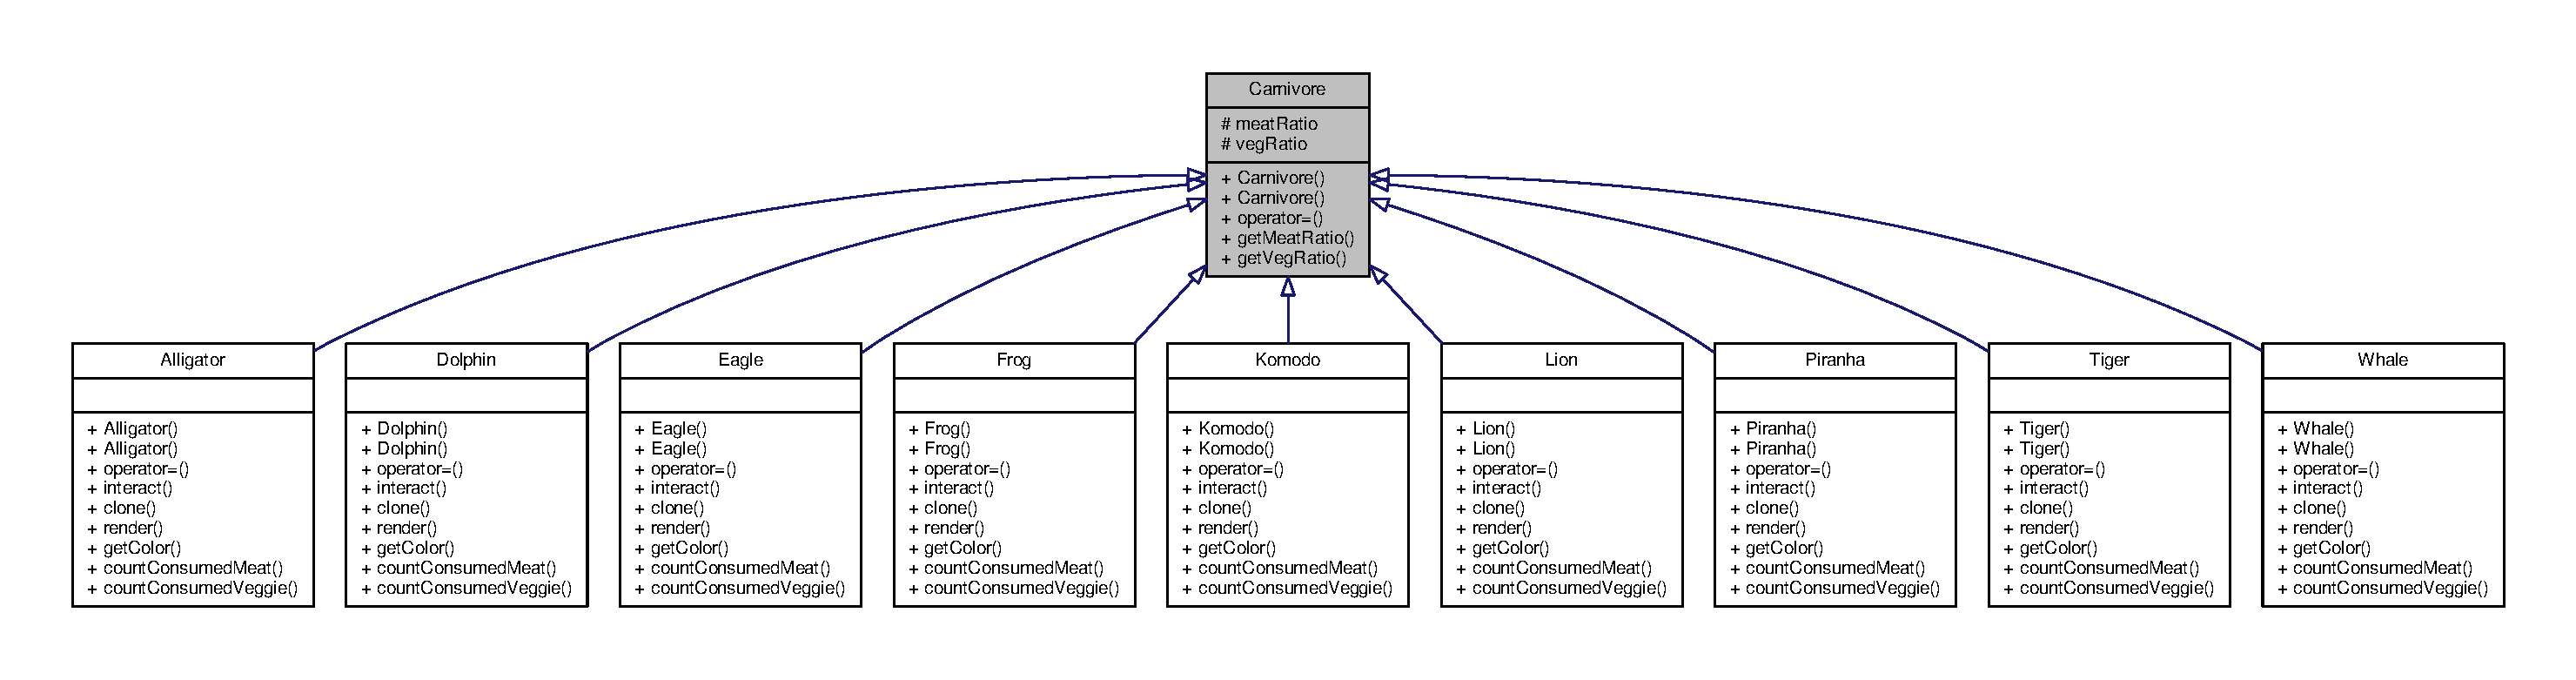
\includegraphics[width=350pt]{classCarnivore__inherit__graph}
\end{center}
\end{figure}


Collaboration diagram for Carnivore\+:
\nopagebreak
\begin{figure}[H]
\begin{center}
\leavevmode
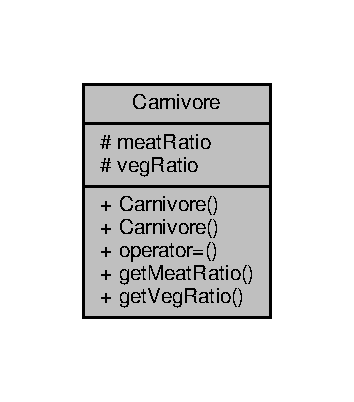
\includegraphics[width=170pt]{classCarnivore__coll__graph}
\end{center}
\end{figure}
\subsection*{Public Member Functions}
\begin{DoxyCompactItemize}
\item 
\hyperlink{classCarnivore_ac18446eeb7acb1dfd3a9c9c955e61ed7}{Carnivore} ()
\begin{DoxyCompactList}\small\item\em Constructor. \end{DoxyCompactList}\item 
\hyperlink{classCarnivore_a32e0695adddbfba360487e31e0653204}{Carnivore} (const \hyperlink{classCarnivore}{Carnivore} \&C)
\begin{DoxyCompactList}\small\item\em Copy Constructor. \end{DoxyCompactList}\item 
\hyperlink{classCarnivore}{Carnivore} \& \hyperlink{classCarnivore_a1f219198f593592d526ba3302d8449f9}{operator=} (const \hyperlink{classCarnivore}{Carnivore} \&C)
\begin{DoxyCompactList}\small\item\em Operator=. Menjamin bukan bitwise copy. \end{DoxyCompactList}\item 
double \hyperlink{classCarnivore_a7d439e225f7cfaf0386c3b1aee77762b}{get\+Meat\+Ratio} () const 
\begin{DoxyCompactList}\small\item\em Getter. Mengembalikan nilai rasio daging. \end{DoxyCompactList}\item 
double \hyperlink{classCarnivore_a74738f03db5bbe83281ada638580dc36}{get\+Veg\+Ratio} () const 
\begin{DoxyCompactList}\small\item\em Getter. Mengembalikan nilai rasio daging. \end{DoxyCompactList}\end{DoxyCompactItemize}
\subsection*{Protected Attributes}
\begin{DoxyCompactItemize}
\item 
double \hyperlink{classCarnivore_a7fded43c2f22eab35e2e6f16ae155f27}{meat\+Ratio}
\item 
const double \hyperlink{classCarnivore_ab4047f87dae34ec4667f42e1efd57d93}{veg\+Ratio} = 0.\+0
\end{DoxyCompactItemize}


\subsection{Detailed Description}
Kelas untuk hewan karnivora (pemakan daging) 

\subsection{Constructor \& Destructor Documentation}
\index{Carnivore@{Carnivore}!Carnivore@{Carnivore}}
\index{Carnivore@{Carnivore}!Carnivore@{Carnivore}}
\subsubsection[{\texorpdfstring{Carnivore()}{Carnivore()}}]{\setlength{\rightskip}{0pt plus 5cm}Carnivore\+::\+Carnivore (
\begin{DoxyParamCaption}
{}
\end{DoxyParamCaption}
)}\hypertarget{classCarnivore_ac18446eeb7acb1dfd3a9c9c955e61ed7}{}\label{classCarnivore_ac18446eeb7acb1dfd3a9c9c955e61ed7}


Constructor. 

\index{Carnivore@{Carnivore}!Carnivore@{Carnivore}}
\index{Carnivore@{Carnivore}!Carnivore@{Carnivore}}
\subsubsection[{\texorpdfstring{Carnivore(const Carnivore \&\+C)}{Carnivore(const Carnivore &C)}}]{\setlength{\rightskip}{0pt plus 5cm}Carnivore\+::\+Carnivore (
\begin{DoxyParamCaption}
\item[{const {\bf Carnivore} \&}]{C}
\end{DoxyParamCaption}
)}\hypertarget{classCarnivore_a32e0695adddbfba360487e31e0653204}{}\label{classCarnivore_a32e0695adddbfba360487e31e0653204}


Copy Constructor. 


\begin{DoxyParams}{Parameters}
{\em \hyperlink{classCarnivore}{Carnivore}} & C yang diacu cctor \\
\hline
\end{DoxyParams}


\subsection{Member Function Documentation}
\index{Carnivore@{Carnivore}!get\+Meat\+Ratio@{get\+Meat\+Ratio}}
\index{get\+Meat\+Ratio@{get\+Meat\+Ratio}!Carnivore@{Carnivore}}
\subsubsection[{\texorpdfstring{get\+Meat\+Ratio() const }{getMeatRatio() const }}]{\setlength{\rightskip}{0pt plus 5cm}double Carnivore\+::get\+Meat\+Ratio (
\begin{DoxyParamCaption}
{}
\end{DoxyParamCaption}
) const}\hypertarget{classCarnivore_a7d439e225f7cfaf0386c3b1aee77762b}{}\label{classCarnivore_a7d439e225f7cfaf0386c3b1aee77762b}


Getter. Mengembalikan nilai rasio daging. 

\begin{DoxyReturn}{Returns}
nilai rasio daging 
\end{DoxyReturn}
\index{Carnivore@{Carnivore}!get\+Veg\+Ratio@{get\+Veg\+Ratio}}
\index{get\+Veg\+Ratio@{get\+Veg\+Ratio}!Carnivore@{Carnivore}}
\subsubsection[{\texorpdfstring{get\+Veg\+Ratio() const }{getVegRatio() const }}]{\setlength{\rightskip}{0pt plus 5cm}double Carnivore\+::get\+Veg\+Ratio (
\begin{DoxyParamCaption}
{}
\end{DoxyParamCaption}
) const}\hypertarget{classCarnivore_a74738f03db5bbe83281ada638580dc36}{}\label{classCarnivore_a74738f03db5bbe83281ada638580dc36}


Getter. Mengembalikan nilai rasio daging. 

\begin{DoxyReturn}{Returns}
nilai rasio sayur 
\end{DoxyReturn}
\index{Carnivore@{Carnivore}!operator=@{operator=}}
\index{operator=@{operator=}!Carnivore@{Carnivore}}
\subsubsection[{\texorpdfstring{operator=(const Carnivore \&\+C)}{operator=(const Carnivore &C)}}]{\setlength{\rightskip}{0pt plus 5cm}{\bf Carnivore} \& Carnivore\+::operator= (
\begin{DoxyParamCaption}
\item[{const {\bf Carnivore} \&}]{C}
\end{DoxyParamCaption}
)}\hypertarget{classCarnivore_a1f219198f593592d526ba3302d8449f9}{}\label{classCarnivore_a1f219198f593592d526ba3302d8449f9}


Operator=. Menjamin bukan bitwise copy. 


\begin{DoxyParams}{Parameters}
{\em C} & \hyperlink{classCarnivore}{Carnivore} berisi data untuk diassign \\
\hline
\end{DoxyParams}


\subsection{Member Data Documentation}
\index{Carnivore@{Carnivore}!meat\+Ratio@{meat\+Ratio}}
\index{meat\+Ratio@{meat\+Ratio}!Carnivore@{Carnivore}}
\subsubsection[{\texorpdfstring{meat\+Ratio}{meatRatio}}]{\setlength{\rightskip}{0pt plus 5cm}double Carnivore\+::meat\+Ratio\hspace{0.3cm}{\ttfamily [protected]}}\hypertarget{classCarnivore_a7fded43c2f22eab35e2e6f16ae155f27}{}\label{classCarnivore_a7fded43c2f22eab35e2e6f16ae155f27}
\index{Carnivore@{Carnivore}!veg\+Ratio@{veg\+Ratio}}
\index{veg\+Ratio@{veg\+Ratio}!Carnivore@{Carnivore}}
\subsubsection[{\texorpdfstring{veg\+Ratio}{vegRatio}}]{\setlength{\rightskip}{0pt plus 5cm}const double Carnivore\+::veg\+Ratio = 0.\+0\hspace{0.3cm}{\ttfamily [protected]}}\hypertarget{classCarnivore_ab4047f87dae34ec4667f42e1efd57d93}{}\label{classCarnivore_ab4047f87dae34ec4667f42e1efd57d93}


The documentation for this class was generated from the following files\+:\begin{DoxyCompactItemize}
\item 
src/renders/animals/diet/\hyperlink{carnivore_8h}{carnivore.\+h}\item 
src/renders/animals/diet/\hyperlink{carnivore_8cpp}{carnivore.\+cpp}\end{DoxyCompactItemize}

\hypertarget{classCell}{}\section{Cell Class Reference}
\label{classCell}\index{Cell@{Cell}}


{\ttfamily \#include $<$cell.\+h$>$}



Inheritance diagram for Cell\+:
\nopagebreak
\begin{figure}[H]
\begin{center}
\leavevmode
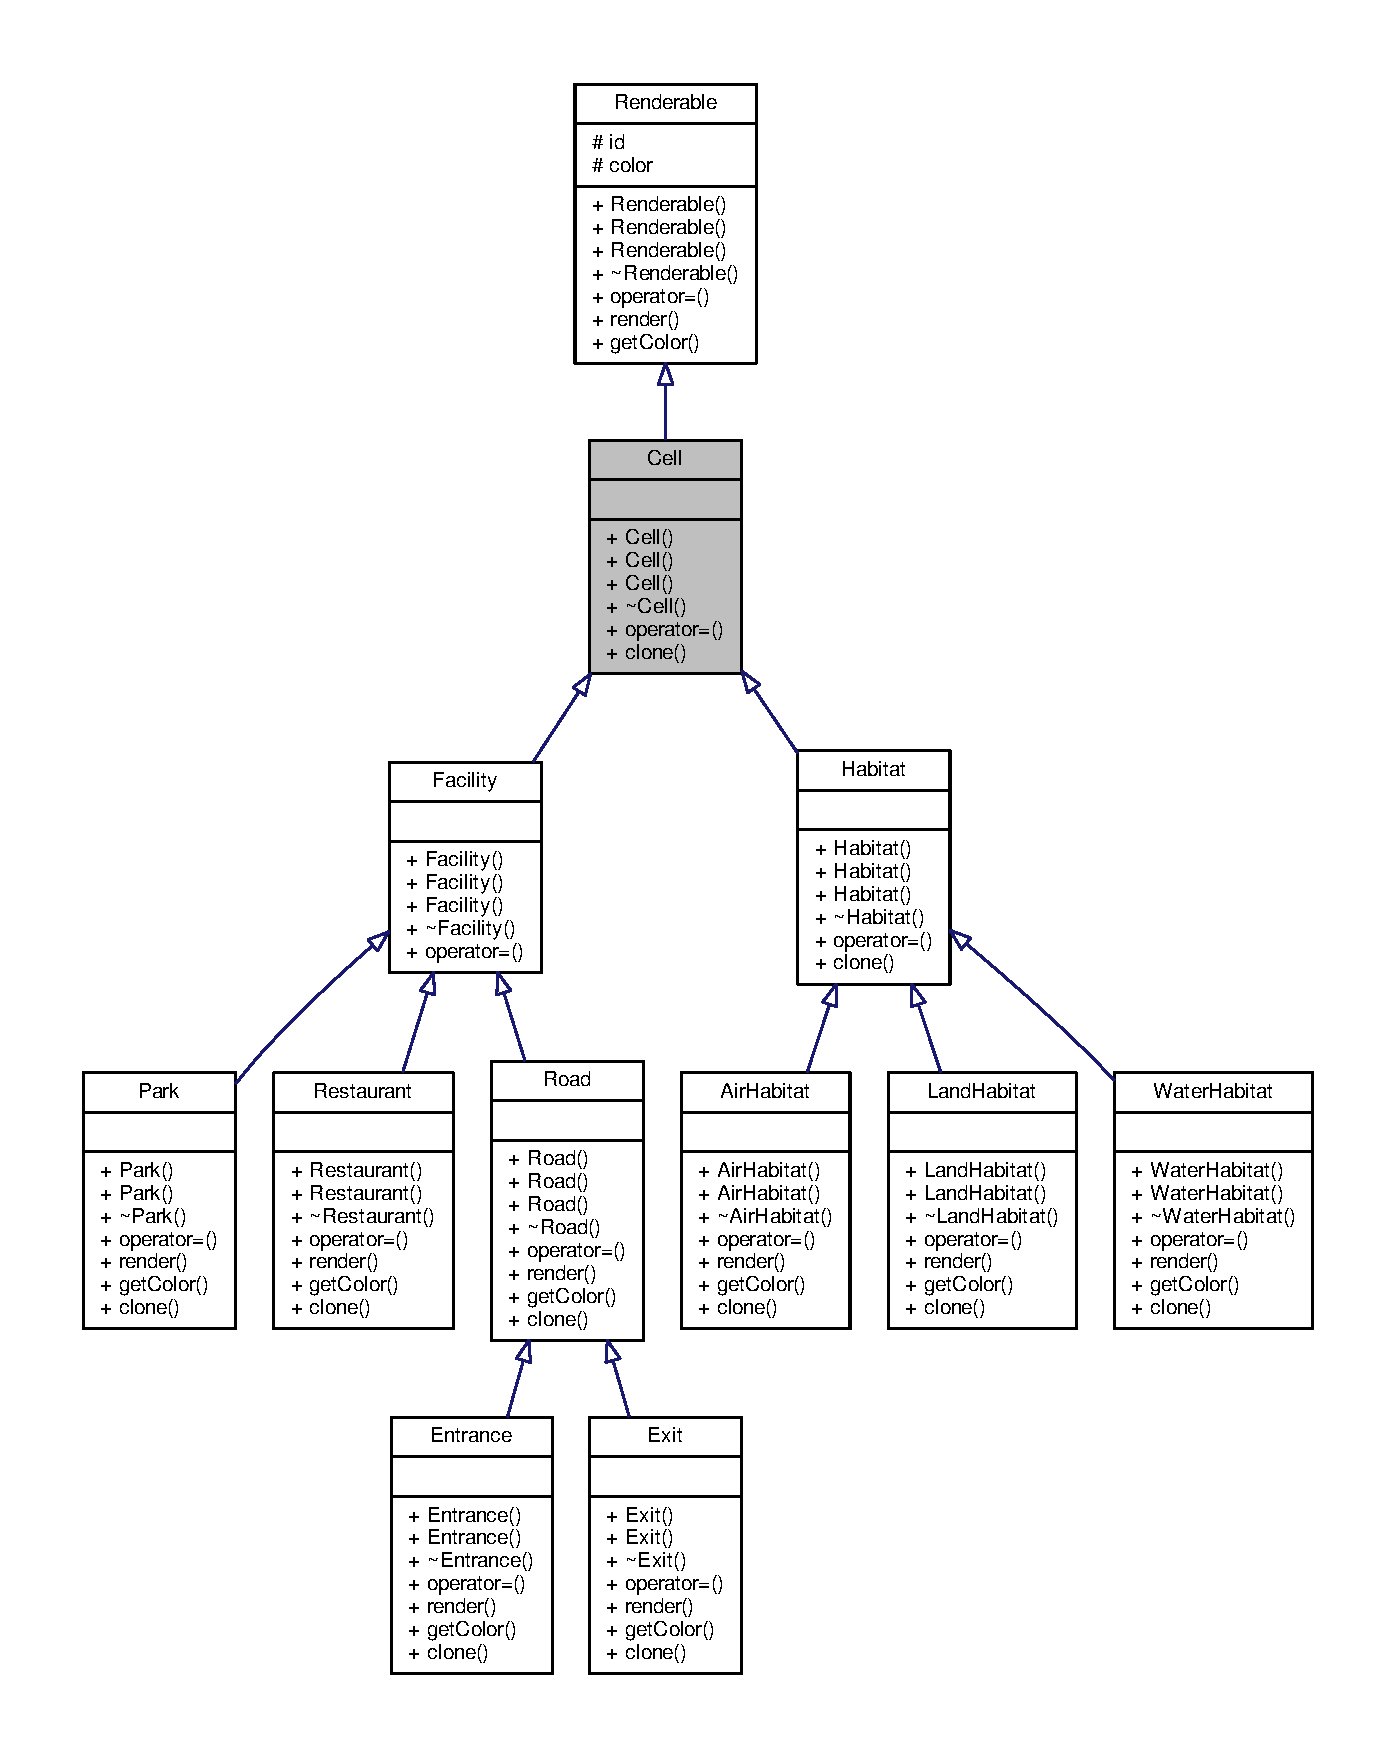
\includegraphics[width=350pt]{classCell__inherit__graph}
\end{center}
\end{figure}


Collaboration diagram for Cell\+:
\nopagebreak
\begin{figure}[H]
\begin{center}
\leavevmode
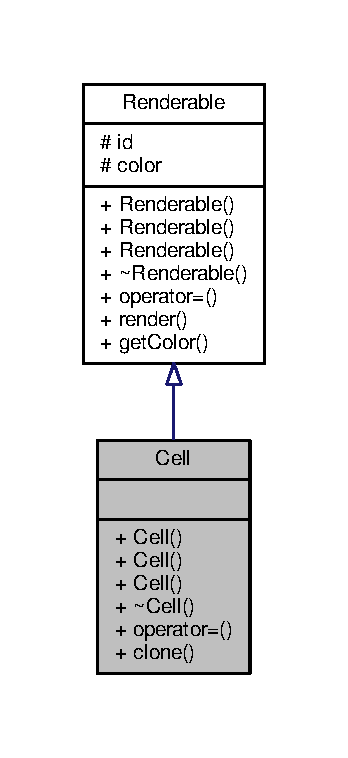
\includegraphics[width=167pt]{classCell__coll__graph}
\end{center}
\end{figure}
\subsection*{Public Member Functions}
\begin{DoxyCompactItemize}
\item 
\hyperlink{classCell_a394510643e8664cf12b5efaf5cb99f71}{Cell} ()
\begin{DoxyCompactList}\small\item\em Constructor. Menciptakan \hyperlink{classCell}{Cell} kosong. \end{DoxyCompactList}\item 
\hyperlink{classCell_a86fe9c1022b8f52158e5bc3de3ee7e0c}{Cell} (char \+\_\+id, \hyperlink{color_8h_ab87bacfdad76e61b9412d7124be44c1c}{Color} \+\_\+color)
\begin{DoxyCompactList}\small\item\em Constructor dengan parameter. Menciptakan \hyperlink{classCell}{Cell} dengan parameter id dan color. \end{DoxyCompactList}\item 
\hyperlink{classCell_a8ca000885181236a713963c5c8bdb46f}{Cell} (const \hyperlink{classCell}{Cell} \&)
\begin{DoxyCompactList}\small\item\em Copy Constructor. Menciptakan salinan dari \hyperlink{classCell}{Cell}. \end{DoxyCompactList}\item 
virtual \hyperlink{classCell_a9fa559f7a28e2b4336c6879ca09304d8}{$\sim$\+Cell} ()
\begin{DoxyCompactList}\small\item\em Destructor. \end{DoxyCompactList}\item 
\hyperlink{classCell}{Cell} \& \hyperlink{classCell_a1c8f1c38098f3b4cbf5126bf218b468d}{operator=} (const \hyperlink{classCell}{Cell} \&)
\begin{DoxyCompactList}\small\item\em Operator=. Menginisialisasi \hyperlink{classCell}{Cell} dari \hyperlink{classCell}{Cell} lain. \end{DoxyCompactList}\item 
virtual \hyperlink{classCell}{Cell} $\ast$ \hyperlink{classCell_aafd03896d9a6131f14273752f9fb9815}{clone} () const =0
\begin{DoxyCompactList}\small\item\em clone. Menduplikasi \hyperlink{classCell}{Cell} objek diri sendiri \end{DoxyCompactList}\end{DoxyCompactItemize}
\subsection*{Additional Inherited Members}


\subsection{Detailed Description}
Kelas abstrak yang merepresentasikan satuan unit tempat dari zoo. 

\subsection{Constructor \& Destructor Documentation}
\index{Cell@{Cell}!Cell@{Cell}}
\index{Cell@{Cell}!Cell@{Cell}}
\subsubsection[{\texorpdfstring{Cell()}{Cell()}}]{\setlength{\rightskip}{0pt plus 5cm}Cell\+::\+Cell (
\begin{DoxyParamCaption}
{}
\end{DoxyParamCaption}
)}\hypertarget{classCell_a394510643e8664cf12b5efaf5cb99f71}{}\label{classCell_a394510643e8664cf12b5efaf5cb99f71}


Constructor. Menciptakan \hyperlink{classCell}{Cell} kosong. 

\index{Cell@{Cell}!Cell@{Cell}}
\index{Cell@{Cell}!Cell@{Cell}}
\subsubsection[{\texorpdfstring{Cell(char \+\_\+id, Color \+\_\+color)}{Cell(char _id, Color _color)}}]{\setlength{\rightskip}{0pt plus 5cm}Cell\+::\+Cell (
\begin{DoxyParamCaption}
\item[{char}]{\+\_\+id, }
\item[{{\bf Color}}]{\+\_\+color}
\end{DoxyParamCaption}
)}\hypertarget{classCell_a86fe9c1022b8f52158e5bc3de3ee7e0c}{}\label{classCell_a86fe9c1022b8f52158e5bc3de3ee7e0c}


Constructor dengan parameter. Menciptakan \hyperlink{classCell}{Cell} dengan parameter id dan color. 


\begin{DoxyParams}{Parameters}
{\em id} & char renderable \\
\hline
{\em color} & warna renderable \\
\hline
\end{DoxyParams}
\index{Cell@{Cell}!Cell@{Cell}}
\index{Cell@{Cell}!Cell@{Cell}}
\subsubsection[{\texorpdfstring{Cell(const Cell \&)}{Cell(const Cell &)}}]{\setlength{\rightskip}{0pt plus 5cm}Cell\+::\+Cell (
\begin{DoxyParamCaption}
\item[{const {\bf Cell} \&}]{C}
\end{DoxyParamCaption}
)}\hypertarget{classCell_a8ca000885181236a713963c5c8bdb46f}{}\label{classCell_a8ca000885181236a713963c5c8bdb46f}


Copy Constructor. Menciptakan salinan dari \hyperlink{classCell}{Cell}. 


\begin{DoxyParams}{Parameters}
{\em C} & \hyperlink{classCell}{Cell} yang ingin disalin. \\
\hline
\end{DoxyParams}
\index{Cell@{Cell}!````~Cell@{$\sim$\+Cell}}
\index{````~Cell@{$\sim$\+Cell}!Cell@{Cell}}
\subsubsection[{\texorpdfstring{$\sim$\+Cell()}{~Cell()}}]{\setlength{\rightskip}{0pt plus 5cm}Cell\+::$\sim$\+Cell (
\begin{DoxyParamCaption}
{}
\end{DoxyParamCaption}
)\hspace{0.3cm}{\ttfamily [virtual]}}\hypertarget{classCell_a9fa559f7a28e2b4336c6879ca09304d8}{}\label{classCell_a9fa559f7a28e2b4336c6879ca09304d8}


Destructor. 



\subsection{Member Function Documentation}
\index{Cell@{Cell}!clone@{clone}}
\index{clone@{clone}!Cell@{Cell}}
\subsubsection[{\texorpdfstring{clone() const =0}{clone() const =0}}]{\setlength{\rightskip}{0pt plus 5cm}virtual {\bf Cell}$\ast$ Cell\+::clone (
\begin{DoxyParamCaption}
{}
\end{DoxyParamCaption}
) const\hspace{0.3cm}{\ttfamily [pure virtual]}}\hypertarget{classCell_aafd03896d9a6131f14273752f9fb9815}{}\label{classCell_aafd03896d9a6131f14273752f9fb9815}


clone. Menduplikasi \hyperlink{classCell}{Cell} objek diri sendiri 

\begin{DoxyReturn}{Returns}
\hyperlink{classCell}{Cell} yang sudah diduplikasi. 
\end{DoxyReturn}


Implemented in \hyperlink{classRoad_a0dae048f0e2f56afa5e3fda6f30bf262}{Road}, \hyperlink{classPark_a94b4494ebee327cbee81ca6b95d11532}{Park}, \hyperlink{classRestaurant_a8189dd83d787840811b90c2c5dbafda0}{Restaurant}, \hyperlink{classEntrance_a5f20360c5b495b5ed4163deb33ff06de}{Entrance}, \hyperlink{classExit_a01a14491e2f7148b0e03b4297c60a0a0}{Exit}, \hyperlink{classAirHabitat_ab756521fcd5adca0283e9bfd0d0fd075}{Air\+Habitat}, \hyperlink{classLandHabitat_add986b725e19b857d3e3fa66689cda73}{Land\+Habitat}, \hyperlink{classWaterHabitat_ab55d7a09373090cfafac504bc1431878}{Water\+Habitat}, and \hyperlink{classHabitat_a640c071c99dbd3dc9cbf4971dbcaa463}{Habitat}.

\index{Cell@{Cell}!operator=@{operator=}}
\index{operator=@{operator=}!Cell@{Cell}}
\subsubsection[{\texorpdfstring{operator=(const Cell \&)}{operator=(const Cell &)}}]{\setlength{\rightskip}{0pt plus 5cm}{\bf Cell} \& Cell\+::operator= (
\begin{DoxyParamCaption}
\item[{const {\bf Cell} \&}]{C}
\end{DoxyParamCaption}
)}\hypertarget{classCell_a1c8f1c38098f3b4cbf5126bf218b468d}{}\label{classCell_a1c8f1c38098f3b4cbf5126bf218b468d}


Operator=. Menginisialisasi \hyperlink{classCell}{Cell} dari \hyperlink{classCell}{Cell} lain. 


\begin{DoxyParams}{Parameters}
{\em C} & \hyperlink{classCell}{Cell} yang akan dicopy \\
\hline
\end{DoxyParams}
\begin{DoxyReturn}{Returns}
\hyperlink{classCell}{Cell} current object yang sudah diassign dengan C 
\end{DoxyReturn}


The documentation for this class was generated from the following files\+:\begin{DoxyCompactItemize}
\item 
src/renders/\hyperlink{cell_8h}{cell.\+h}\item 
src/renders/\hyperlink{cell_8cpp}{cell.\+cpp}\end{DoxyCompactItemize}

\hypertarget{classCendrawasih}{}\section{Cendrawasih Class Reference}
\label{classCendrawasih}\index{Cendrawasih@{Cendrawasih}}


{\ttfamily \#include $<$species.\+h$>$}



Inheritance diagram for Cendrawasih\+:
\nopagebreak
\begin{figure}[H]
\begin{center}
\leavevmode
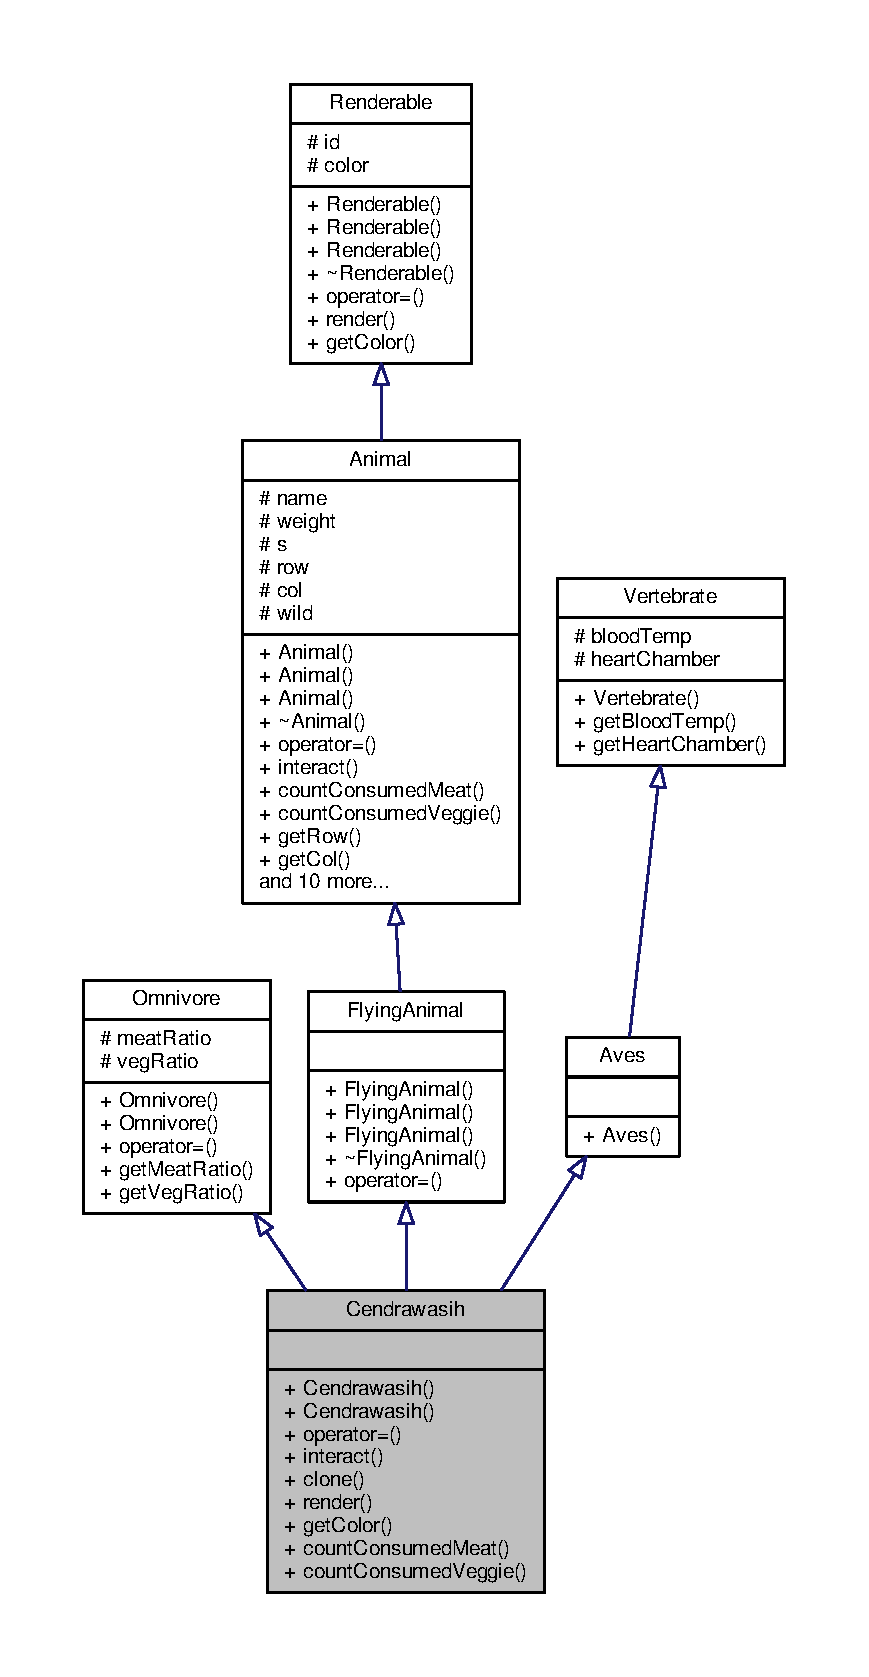
\includegraphics[height=550pt]{classCendrawasih__inherit__graph}
\end{center}
\end{figure}


Collaboration diagram for Cendrawasih\+:
\nopagebreak
\begin{figure}[H]
\begin{center}
\leavevmode
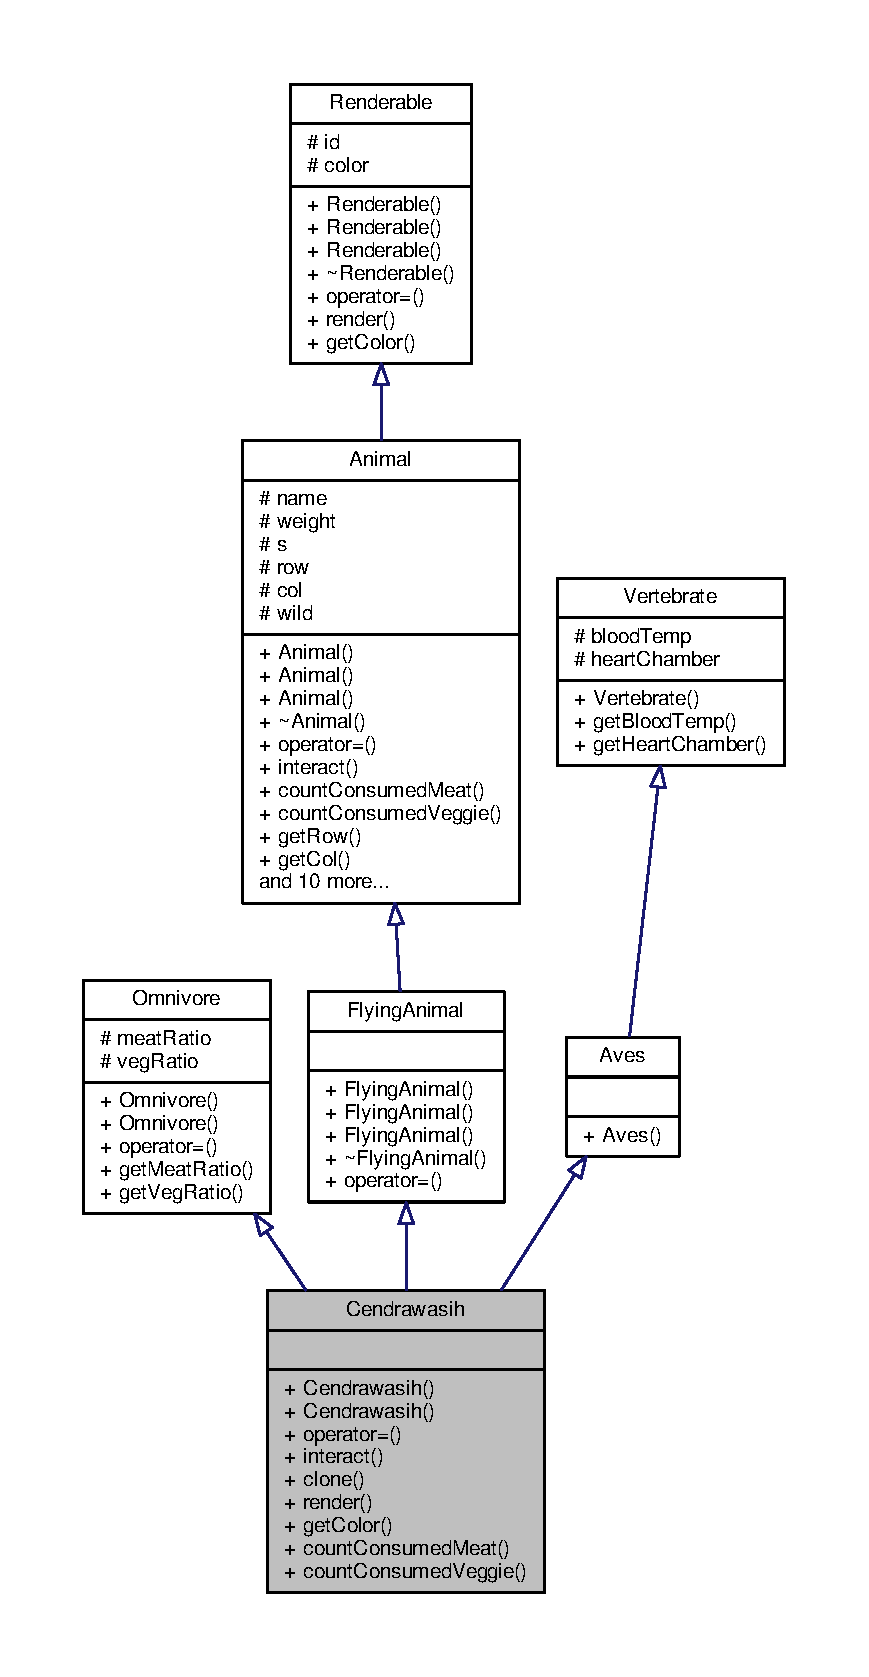
\includegraphics[height=550pt]{classCendrawasih__coll__graph}
\end{center}
\end{figure}
\subsection*{Public Member Functions}
\begin{DoxyCompactItemize}
\item 
\hyperlink{classCendrawasih_abf454396e2e763de85b2529c58c5e550}{Cendrawasih} (string \+\_\+name, double \+\_\+weight, \hyperlink{sex_8h_a2633cb393c68bb2ee8080db58fb7ba93}{Sex} \+\_\+s, int \+\_\+r, int \+\_\+c)
\begin{DoxyCompactList}\small\item\em Consructor. \end{DoxyCompactList}\item 
\hyperlink{classCendrawasih_aa224bbf2b313972f0f4fc18a640d1a8a}{Cendrawasih} (const \hyperlink{classCendrawasih}{Cendrawasih} \&C)
\begin{DoxyCompactList}\small\item\em Copy Consructor. \end{DoxyCompactList}\item 
\hyperlink{classCendrawasih}{Cendrawasih} \& \hyperlink{classCendrawasih_ac96cdea48fe452c5ee2c8af7640fa15e}{operator=} (const \hyperlink{classCendrawasih}{Cendrawasih} \&C)
\begin{DoxyCompactList}\small\item\em Operator=. Melakukan assignment pada objek. \end{DoxyCompactList}\item 
virtual void \hyperlink{classCendrawasih_ab24c4c34838000da51a810dec7d29669}{interact} ()
\begin{DoxyCompactList}\small\item\em interact. Menampilkan interaksi hewan ke layar \end{DoxyCompactList}\item 
virtual \hyperlink{classCendrawasih}{Cendrawasih} $\ast$ \hyperlink{classCendrawasih_a39cf4d2c4a8008a0d6e1292f1cbb86b2}{clone} () const 
\begin{DoxyCompactList}\small\item\em clone Menduplikat diri sendiri \end{DoxyCompactList}\item 
virtual char \hyperlink{classCendrawasih_aa669346ff22d3fb1c2df2f4e3170356d}{render} ()
\begin{DoxyCompactList}\small\item\em render Mengembalikan karakter id tiap hewan \end{DoxyCompactList}\item 
virtual \hyperlink{color_8h_ab87bacfdad76e61b9412d7124be44c1c}{Color} \hyperlink{classCendrawasih_aa042342a8a9b78489e049a5e31e36770}{get\+Color} ()
\begin{DoxyCompactList}\small\item\em get\+Color Mengembalikan warna dari hewan \end{DoxyCompactList}\item 
virtual double \hyperlink{classCendrawasih_a899bcc2043226dc51f77f02c644f7c3f}{count\+Consumed\+Meat} ()
\begin{DoxyCompactList}\small\item\em count\+Consumed\+Meat Mengembalikan jumlah daging yang dikonsumsi \end{DoxyCompactList}\item 
virtual double \hyperlink{classCendrawasih_ae3e380084d6e7e9574d2bdb439155ccc}{count\+Consumed\+Veggie} ()
\begin{DoxyCompactList}\small\item\em count\+Consumed\+Veggie Mengembalikan jumlah makanan tumbuhan yang dikonsumsi \end{DoxyCompactList}\end{DoxyCompactItemize}
\subsection*{Additional Inherited Members}


\subsection{Constructor \& Destructor Documentation}
\index{Cendrawasih@{Cendrawasih}!Cendrawasih@{Cendrawasih}}
\index{Cendrawasih@{Cendrawasih}!Cendrawasih@{Cendrawasih}}
\subsubsection[{\texorpdfstring{Cendrawasih(string \+\_\+name, double \+\_\+weight, Sex \+\_\+s, int \+\_\+r, int \+\_\+c)}{Cendrawasih(string _name, double _weight, Sex _s, int _r, int _c)}}]{\setlength{\rightskip}{0pt plus 5cm}Cendrawasih\+::\+Cendrawasih (
\begin{DoxyParamCaption}
\item[{string}]{\+\_\+name, }
\item[{double}]{\+\_\+weight, }
\item[{{\bf Sex}}]{\+\_\+s, }
\item[{int}]{\+\_\+r, }
\item[{int}]{\+\_\+c}
\end{DoxyParamCaption}
)}\hypertarget{classCendrawasih_abf454396e2e763de85b2529c58c5e550}{}\label{classCendrawasih_abf454396e2e763de85b2529c58c5e550}


Consructor. 


\begin{DoxyParams}{Parameters}
{\em \+\_\+name} & nama binatang \\
\hline
{\em \+\_\+weight} & berat \\
\hline
{\em \+\_\+s} & jenis kelamin \\
\hline
\end{DoxyParams}
\index{Cendrawasih@{Cendrawasih}!Cendrawasih@{Cendrawasih}}
\index{Cendrawasih@{Cendrawasih}!Cendrawasih@{Cendrawasih}}
\subsubsection[{\texorpdfstring{Cendrawasih(const Cendrawasih \&\+C)}{Cendrawasih(const Cendrawasih &C)}}]{\setlength{\rightskip}{0pt plus 5cm}Cendrawasih\+::\+Cendrawasih (
\begin{DoxyParamCaption}
\item[{const {\bf Cendrawasih} \&}]{C}
\end{DoxyParamCaption}
)}\hypertarget{classCendrawasih_aa224bbf2b313972f0f4fc18a640d1a8a}{}\label{classCendrawasih_aa224bbf2b313972f0f4fc18a640d1a8a}


Copy Consructor. 


\begin{DoxyParams}{Parameters}
{\em C} & objek yang akan disalin \\
\hline
\end{DoxyParams}


\subsection{Member Function Documentation}
\index{Cendrawasih@{Cendrawasih}!clone@{clone}}
\index{clone@{clone}!Cendrawasih@{Cendrawasih}}
\subsubsection[{\texorpdfstring{clone() const }{clone() const }}]{\setlength{\rightskip}{0pt plus 5cm}{\bf Cendrawasih} $\ast$ Cendrawasih\+::clone (
\begin{DoxyParamCaption}
{}
\end{DoxyParamCaption}
) const\hspace{0.3cm}{\ttfamily [virtual]}}\hypertarget{classCendrawasih_a39cf4d2c4a8008a0d6e1292f1cbb86b2}{}\label{classCendrawasih_a39cf4d2c4a8008a0d6e1292f1cbb86b2}


clone Menduplikat diri sendiri 

\begin{DoxyReturn}{Returns}
value object hasil kloning 
\end{DoxyReturn}


Implements \hyperlink{classAnimal_a1430e040ea4ff43bc453fa0ad19c308d}{Animal}.

\index{Cendrawasih@{Cendrawasih}!count\+Consumed\+Meat@{count\+Consumed\+Meat}}
\index{count\+Consumed\+Meat@{count\+Consumed\+Meat}!Cendrawasih@{Cendrawasih}}
\subsubsection[{\texorpdfstring{count\+Consumed\+Meat()}{countConsumedMeat()}}]{\setlength{\rightskip}{0pt plus 5cm}double Cendrawasih\+::count\+Consumed\+Meat (
\begin{DoxyParamCaption}
{}
\end{DoxyParamCaption}
)\hspace{0.3cm}{\ttfamily [virtual]}}\hypertarget{classCendrawasih_a899bcc2043226dc51f77f02c644f7c3f}{}\label{classCendrawasih_a899bcc2043226dc51f77f02c644f7c3f}


count\+Consumed\+Meat Mengembalikan jumlah daging yang dikonsumsi 

\begin{DoxyReturn}{Returns}
jumlah daging yang dikonsumsi 
\end{DoxyReturn}


Implements \hyperlink{classAnimal_a84ccc380d237650f2bf24d792627d376}{Animal}.

\index{Cendrawasih@{Cendrawasih}!count\+Consumed\+Veggie@{count\+Consumed\+Veggie}}
\index{count\+Consumed\+Veggie@{count\+Consumed\+Veggie}!Cendrawasih@{Cendrawasih}}
\subsubsection[{\texorpdfstring{count\+Consumed\+Veggie()}{countConsumedVeggie()}}]{\setlength{\rightskip}{0pt plus 5cm}double Cendrawasih\+::count\+Consumed\+Veggie (
\begin{DoxyParamCaption}
{}
\end{DoxyParamCaption}
)\hspace{0.3cm}{\ttfamily [virtual]}}\hypertarget{classCendrawasih_ae3e380084d6e7e9574d2bdb439155ccc}{}\label{classCendrawasih_ae3e380084d6e7e9574d2bdb439155ccc}


count\+Consumed\+Veggie Mengembalikan jumlah makanan tumbuhan yang dikonsumsi 

\begin{DoxyReturn}{Returns}
jumlah makanan tumbuhan yang dikonsumsi 
\end{DoxyReturn}


Implements \hyperlink{classAnimal_aaa7e4bdb7f5a10060b6dcaf09215f822}{Animal}.

\index{Cendrawasih@{Cendrawasih}!get\+Color@{get\+Color}}
\index{get\+Color@{get\+Color}!Cendrawasih@{Cendrawasih}}
\subsubsection[{\texorpdfstring{get\+Color()}{getColor()}}]{\setlength{\rightskip}{0pt plus 5cm}{\bf Color} Cendrawasih\+::get\+Color (
\begin{DoxyParamCaption}
{}
\end{DoxyParamCaption}
)\hspace{0.3cm}{\ttfamily [virtual]}}\hypertarget{classCendrawasih_aa042342a8a9b78489e049a5e31e36770}{}\label{classCendrawasih_aa042342a8a9b78489e049a5e31e36770}


get\+Color Mengembalikan warna dari hewan 

\begin{DoxyReturn}{Returns}
warna cetak hewan 
\end{DoxyReturn}


Implements \hyperlink{classRenderable_ab3bcc93b20929c6e92b64223344a73d5}{Renderable}.

\index{Cendrawasih@{Cendrawasih}!interact@{interact}}
\index{interact@{interact}!Cendrawasih@{Cendrawasih}}
\subsubsection[{\texorpdfstring{interact()}{interact()}}]{\setlength{\rightskip}{0pt plus 5cm}void Cendrawasih\+::interact (
\begin{DoxyParamCaption}
{}
\end{DoxyParamCaption}
)\hspace{0.3cm}{\ttfamily [virtual]}}\hypertarget{classCendrawasih_ab24c4c34838000da51a810dec7d29669}{}\label{classCendrawasih_ab24c4c34838000da51a810dec7d29669}


interact. Menampilkan interaksi hewan ke layar 



Implements \hyperlink{classAnimal_af47626b050b665e9a19525227d2b840f}{Animal}.

\index{Cendrawasih@{Cendrawasih}!operator=@{operator=}}
\index{operator=@{operator=}!Cendrawasih@{Cendrawasih}}
\subsubsection[{\texorpdfstring{operator=(const Cendrawasih \&\+C)}{operator=(const Cendrawasih &C)}}]{\setlength{\rightskip}{0pt plus 5cm}{\bf Cendrawasih} \& Cendrawasih\+::operator= (
\begin{DoxyParamCaption}
\item[{const {\bf Cendrawasih} \&}]{C}
\end{DoxyParamCaption}
)}\hypertarget{classCendrawasih_ac96cdea48fe452c5ee2c8af7640fa15e}{}\label{classCendrawasih_ac96cdea48fe452c5ee2c8af7640fa15e}


Operator=. Melakukan assignment pada objek. 


\begin{DoxyParams}{Parameters}
{\em C} & objek yang akan disalin \\
\hline
\end{DoxyParams}
\index{Cendrawasih@{Cendrawasih}!render@{render}}
\index{render@{render}!Cendrawasih@{Cendrawasih}}
\subsubsection[{\texorpdfstring{render()}{render()}}]{\setlength{\rightskip}{0pt plus 5cm}char Cendrawasih\+::render (
\begin{DoxyParamCaption}
{}
\end{DoxyParamCaption}
)\hspace{0.3cm}{\ttfamily [virtual]}}\hypertarget{classCendrawasih_aa669346ff22d3fb1c2df2f4e3170356d}{}\label{classCendrawasih_aa669346ff22d3fb1c2df2f4e3170356d}


render Mengembalikan karakter id tiap hewan 

\begin{DoxyReturn}{Returns}
karakter tiap hewan 
\end{DoxyReturn}


Implements \hyperlink{classRenderable_aafa9280e6dcfa557b3cd675221fd97b4}{Renderable}.



The documentation for this class was generated from the following files\+:\begin{DoxyCompactItemize}
\item 
src/renders/animals/\hyperlink{species_8h}{species.\+h}\item 
src/renders/animals/\hyperlink{species_8cpp}{species.\+cpp}\end{DoxyCompactItemize}

\hypertarget{classChimpanzee}{}\section{Chimpanzee Class Reference}
\label{classChimpanzee}\index{Chimpanzee@{Chimpanzee}}


{\ttfamily \#include $<$species.\+h$>$}



Inheritance diagram for Chimpanzee\+:
\nopagebreak
\begin{figure}[H]
\begin{center}
\leavevmode
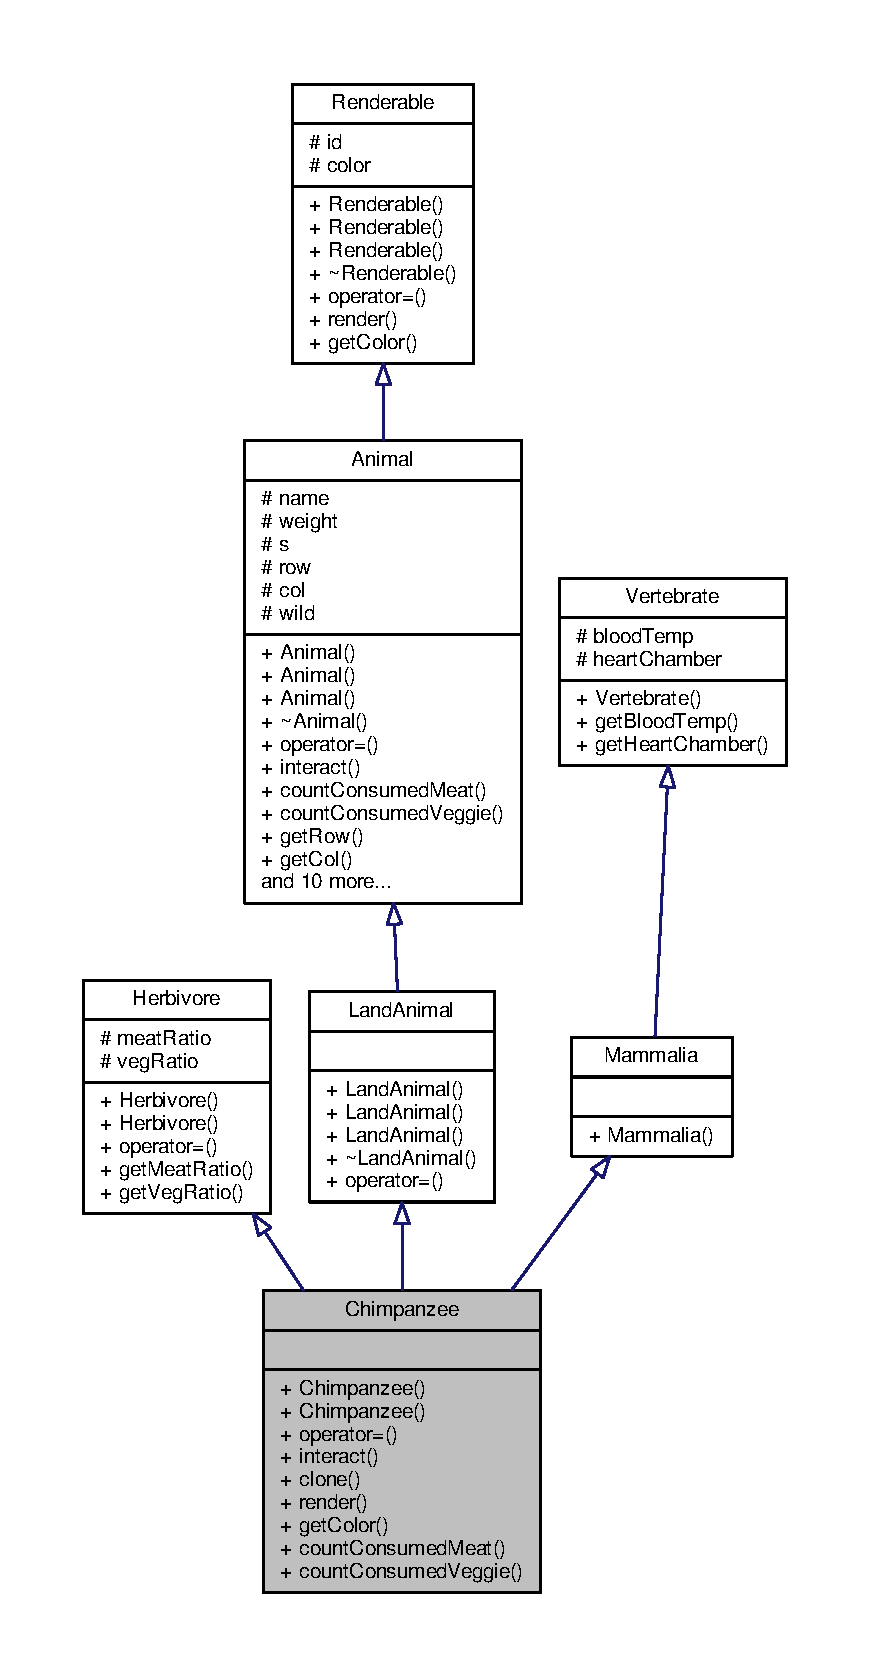
\includegraphics[height=550pt]{classChimpanzee__inherit__graph}
\end{center}
\end{figure}


Collaboration diagram for Chimpanzee\+:
\nopagebreak
\begin{figure}[H]
\begin{center}
\leavevmode
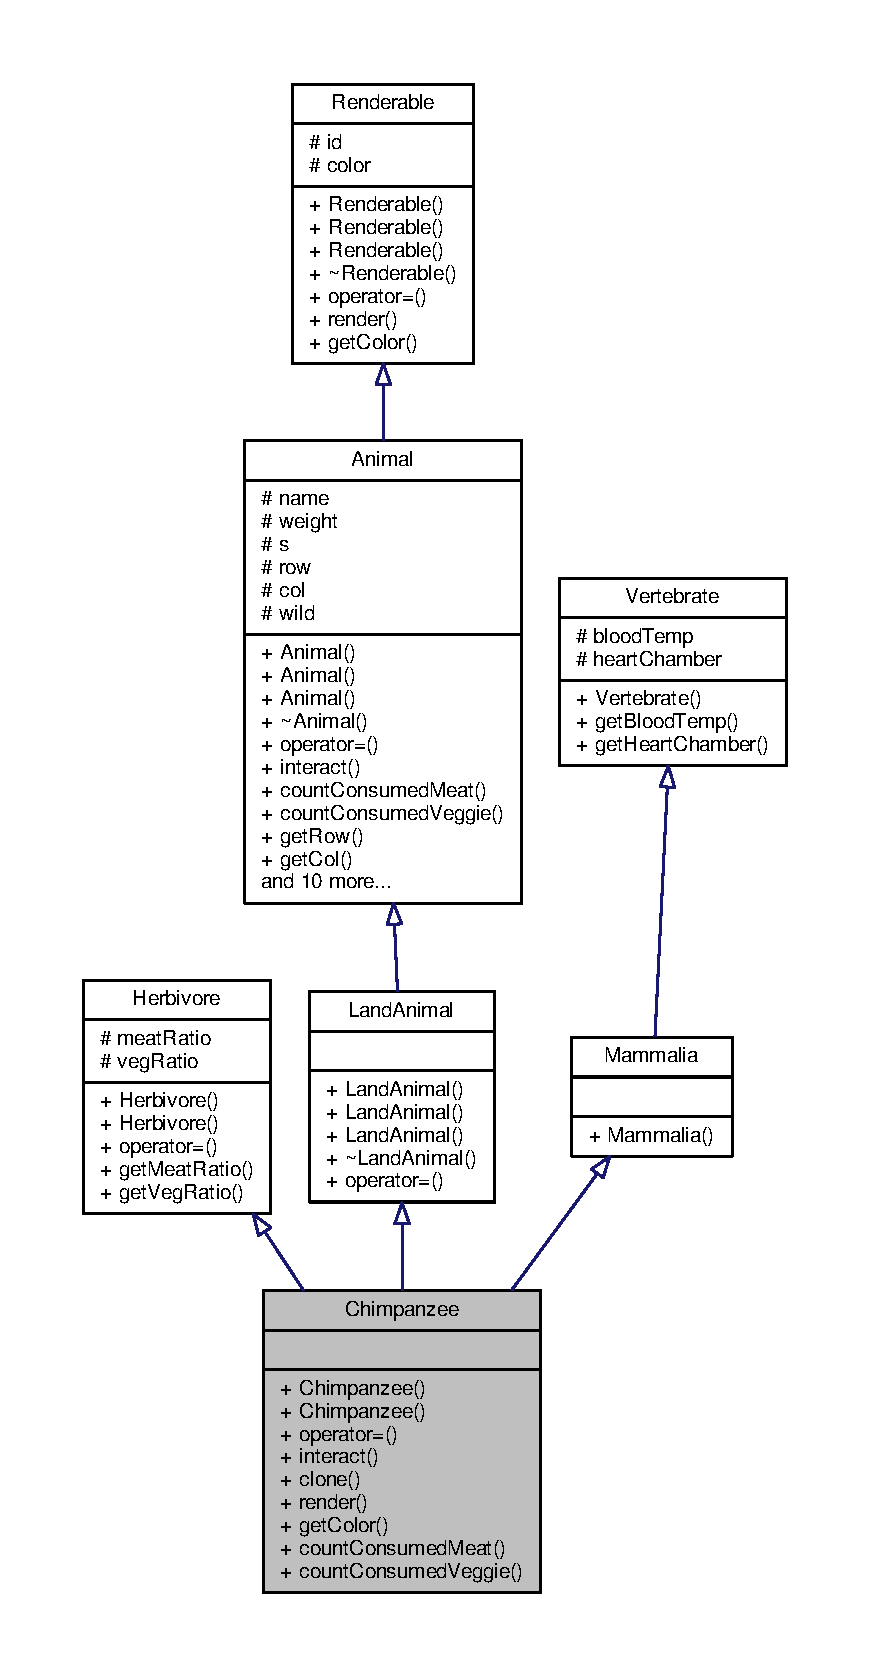
\includegraphics[height=550pt]{classChimpanzee__coll__graph}
\end{center}
\end{figure}
\subsection*{Public Member Functions}
\begin{DoxyCompactItemize}
\item 
\hyperlink{classChimpanzee_a147026737472ddf50fc10f72ad1d8234}{Chimpanzee} (string \+\_\+name, double \+\_\+weight, \hyperlink{sex_8h_a2633cb393c68bb2ee8080db58fb7ba93}{Sex} \+\_\+s, int \+\_\+r, int \+\_\+c)
\begin{DoxyCompactList}\small\item\em Consructor. \end{DoxyCompactList}\item 
\hyperlink{classChimpanzee_a74d8984840f0090f2966d226501bdd92}{Chimpanzee} (const \hyperlink{classChimpanzee}{Chimpanzee} \&C)
\begin{DoxyCompactList}\small\item\em Copy Consructor. \end{DoxyCompactList}\item 
\hyperlink{classChimpanzee}{Chimpanzee} \& \hyperlink{classChimpanzee_a9ad895dc0a2fe9912c948c62f3637844}{operator=} (const \hyperlink{classChimpanzee}{Chimpanzee} \&C)
\begin{DoxyCompactList}\small\item\em Operator=. Melakukan assignment pada objek. \end{DoxyCompactList}\item 
virtual void \hyperlink{classChimpanzee_aade8161c7bcd697eae3d5a3559f6d976}{interact} ()
\begin{DoxyCompactList}\small\item\em interact. Menampilkan interaksi hewan ke layar \end{DoxyCompactList}\item 
virtual \hyperlink{classChimpanzee}{Chimpanzee} $\ast$ \hyperlink{classChimpanzee_ab4e4e896ca7461d22c526e5a86602903}{clone} () const 
\begin{DoxyCompactList}\small\item\em clone Menduplikat diri sendiri \end{DoxyCompactList}\item 
virtual char \hyperlink{classChimpanzee_acad5b9a73a684b44138e842326090357}{render} ()
\begin{DoxyCompactList}\small\item\em render Mengembalikan karakter id tiap hewan \end{DoxyCompactList}\item 
virtual \hyperlink{color_8h_ab87bacfdad76e61b9412d7124be44c1c}{Color} \hyperlink{classChimpanzee_a5160b1aac99d3eb999e88b0e1826724c}{get\+Color} ()
\begin{DoxyCompactList}\small\item\em get\+Color Mengembalikan warna dari hewan \end{DoxyCompactList}\item 
virtual double \hyperlink{classChimpanzee_a7890d585fe43b40b65c5ac68c02bc1a8}{count\+Consumed\+Meat} ()
\begin{DoxyCompactList}\small\item\em count\+Consumed\+Meat Mengembalikan jumlah daging yang dikonsumsi \end{DoxyCompactList}\item 
virtual double \hyperlink{classChimpanzee_a8a9a0561d0eacc5c82fad0ea4e4ed99d}{count\+Consumed\+Veggie} ()
\begin{DoxyCompactList}\small\item\em count\+Consumed\+Veggie Mengembalikan jumlah makanan tumbuhan yang dikonsumsi \end{DoxyCompactList}\end{DoxyCompactItemize}
\subsection*{Additional Inherited Members}


\subsection{Constructor \& Destructor Documentation}
\index{Chimpanzee@{Chimpanzee}!Chimpanzee@{Chimpanzee}}
\index{Chimpanzee@{Chimpanzee}!Chimpanzee@{Chimpanzee}}
\subsubsection[{\texorpdfstring{Chimpanzee(string \+\_\+name, double \+\_\+weight, Sex \+\_\+s, int \+\_\+r, int \+\_\+c)}{Chimpanzee(string _name, double _weight, Sex _s, int _r, int _c)}}]{\setlength{\rightskip}{0pt plus 5cm}Chimpanzee\+::\+Chimpanzee (
\begin{DoxyParamCaption}
\item[{string}]{\+\_\+name, }
\item[{double}]{\+\_\+weight, }
\item[{{\bf Sex}}]{\+\_\+s, }
\item[{int}]{\+\_\+r, }
\item[{int}]{\+\_\+c}
\end{DoxyParamCaption}
)}\hypertarget{classChimpanzee_a147026737472ddf50fc10f72ad1d8234}{}\label{classChimpanzee_a147026737472ddf50fc10f72ad1d8234}


Consructor. 


\begin{DoxyParams}{Parameters}
{\em \+\_\+name} & nama binatang \\
\hline
{\em \+\_\+weight} & berat \\
\hline
{\em \+\_\+s} & jenis kelamin \\
\hline
\end{DoxyParams}
\index{Chimpanzee@{Chimpanzee}!Chimpanzee@{Chimpanzee}}
\index{Chimpanzee@{Chimpanzee}!Chimpanzee@{Chimpanzee}}
\subsubsection[{\texorpdfstring{Chimpanzee(const Chimpanzee \&\+C)}{Chimpanzee(const Chimpanzee &C)}}]{\setlength{\rightskip}{0pt plus 5cm}Chimpanzee\+::\+Chimpanzee (
\begin{DoxyParamCaption}
\item[{const {\bf Chimpanzee} \&}]{C}
\end{DoxyParamCaption}
)}\hypertarget{classChimpanzee_a74d8984840f0090f2966d226501bdd92}{}\label{classChimpanzee_a74d8984840f0090f2966d226501bdd92}


Copy Consructor. 


\begin{DoxyParams}{Parameters}
{\em C} & objek yang akan disalin \\
\hline
\end{DoxyParams}


\subsection{Member Function Documentation}
\index{Chimpanzee@{Chimpanzee}!clone@{clone}}
\index{clone@{clone}!Chimpanzee@{Chimpanzee}}
\subsubsection[{\texorpdfstring{clone() const }{clone() const }}]{\setlength{\rightskip}{0pt plus 5cm}{\bf Chimpanzee} $\ast$ Chimpanzee\+::clone (
\begin{DoxyParamCaption}
{}
\end{DoxyParamCaption}
) const\hspace{0.3cm}{\ttfamily [virtual]}}\hypertarget{classChimpanzee_ab4e4e896ca7461d22c526e5a86602903}{}\label{classChimpanzee_ab4e4e896ca7461d22c526e5a86602903}


clone Menduplikat diri sendiri 

\begin{DoxyReturn}{Returns}
value object hasil kloning 
\end{DoxyReturn}


Implements \hyperlink{classAnimal_a1430e040ea4ff43bc453fa0ad19c308d}{Animal}.

\index{Chimpanzee@{Chimpanzee}!count\+Consumed\+Meat@{count\+Consumed\+Meat}}
\index{count\+Consumed\+Meat@{count\+Consumed\+Meat}!Chimpanzee@{Chimpanzee}}
\subsubsection[{\texorpdfstring{count\+Consumed\+Meat()}{countConsumedMeat()}}]{\setlength{\rightskip}{0pt plus 5cm}double Chimpanzee\+::count\+Consumed\+Meat (
\begin{DoxyParamCaption}
{}
\end{DoxyParamCaption}
)\hspace{0.3cm}{\ttfamily [virtual]}}\hypertarget{classChimpanzee_a7890d585fe43b40b65c5ac68c02bc1a8}{}\label{classChimpanzee_a7890d585fe43b40b65c5ac68c02bc1a8}


count\+Consumed\+Meat Mengembalikan jumlah daging yang dikonsumsi 

\begin{DoxyReturn}{Returns}
jumlah daging yang dikonsumsi 
\end{DoxyReturn}


Implements \hyperlink{classAnimal_a84ccc380d237650f2bf24d792627d376}{Animal}.

\index{Chimpanzee@{Chimpanzee}!count\+Consumed\+Veggie@{count\+Consumed\+Veggie}}
\index{count\+Consumed\+Veggie@{count\+Consumed\+Veggie}!Chimpanzee@{Chimpanzee}}
\subsubsection[{\texorpdfstring{count\+Consumed\+Veggie()}{countConsumedVeggie()}}]{\setlength{\rightskip}{0pt plus 5cm}double Chimpanzee\+::count\+Consumed\+Veggie (
\begin{DoxyParamCaption}
{}
\end{DoxyParamCaption}
)\hspace{0.3cm}{\ttfamily [virtual]}}\hypertarget{classChimpanzee_a8a9a0561d0eacc5c82fad0ea4e4ed99d}{}\label{classChimpanzee_a8a9a0561d0eacc5c82fad0ea4e4ed99d}


count\+Consumed\+Veggie Mengembalikan jumlah makanan tumbuhan yang dikonsumsi 

\begin{DoxyReturn}{Returns}
jumlah makanan tumbuhan yang dikonsumsi 
\end{DoxyReturn}


Implements \hyperlink{classAnimal_aaa7e4bdb7f5a10060b6dcaf09215f822}{Animal}.

\index{Chimpanzee@{Chimpanzee}!get\+Color@{get\+Color}}
\index{get\+Color@{get\+Color}!Chimpanzee@{Chimpanzee}}
\subsubsection[{\texorpdfstring{get\+Color()}{getColor()}}]{\setlength{\rightskip}{0pt plus 5cm}{\bf Color} Chimpanzee\+::get\+Color (
\begin{DoxyParamCaption}
{}
\end{DoxyParamCaption}
)\hspace{0.3cm}{\ttfamily [virtual]}}\hypertarget{classChimpanzee_a5160b1aac99d3eb999e88b0e1826724c}{}\label{classChimpanzee_a5160b1aac99d3eb999e88b0e1826724c}


get\+Color Mengembalikan warna dari hewan 

\begin{DoxyReturn}{Returns}
warna cetak hewan 
\end{DoxyReturn}


Implements \hyperlink{classRenderable_ab3bcc93b20929c6e92b64223344a73d5}{Renderable}.

\index{Chimpanzee@{Chimpanzee}!interact@{interact}}
\index{interact@{interact}!Chimpanzee@{Chimpanzee}}
\subsubsection[{\texorpdfstring{interact()}{interact()}}]{\setlength{\rightskip}{0pt plus 5cm}void Chimpanzee\+::interact (
\begin{DoxyParamCaption}
{}
\end{DoxyParamCaption}
)\hspace{0.3cm}{\ttfamily [virtual]}}\hypertarget{classChimpanzee_aade8161c7bcd697eae3d5a3559f6d976}{}\label{classChimpanzee_aade8161c7bcd697eae3d5a3559f6d976}


interact. Menampilkan interaksi hewan ke layar 



Implements \hyperlink{classAnimal_af47626b050b665e9a19525227d2b840f}{Animal}.

\index{Chimpanzee@{Chimpanzee}!operator=@{operator=}}
\index{operator=@{operator=}!Chimpanzee@{Chimpanzee}}
\subsubsection[{\texorpdfstring{operator=(const Chimpanzee \&\+C)}{operator=(const Chimpanzee &C)}}]{\setlength{\rightskip}{0pt plus 5cm}{\bf Chimpanzee} \& Chimpanzee\+::operator= (
\begin{DoxyParamCaption}
\item[{const {\bf Chimpanzee} \&}]{C}
\end{DoxyParamCaption}
)}\hypertarget{classChimpanzee_a9ad895dc0a2fe9912c948c62f3637844}{}\label{classChimpanzee_a9ad895dc0a2fe9912c948c62f3637844}


Operator=. Melakukan assignment pada objek. 


\begin{DoxyParams}{Parameters}
{\em C} & objek yang akan disalin \\
\hline
\end{DoxyParams}
\index{Chimpanzee@{Chimpanzee}!render@{render}}
\index{render@{render}!Chimpanzee@{Chimpanzee}}
\subsubsection[{\texorpdfstring{render()}{render()}}]{\setlength{\rightskip}{0pt plus 5cm}char Chimpanzee\+::render (
\begin{DoxyParamCaption}
{}
\end{DoxyParamCaption}
)\hspace{0.3cm}{\ttfamily [virtual]}}\hypertarget{classChimpanzee_acad5b9a73a684b44138e842326090357}{}\label{classChimpanzee_acad5b9a73a684b44138e842326090357}


render Mengembalikan karakter id tiap hewan 

\begin{DoxyReturn}{Returns}
karakter tiap hewan 
\end{DoxyReturn}


Implements \hyperlink{classRenderable_aafa9280e6dcfa557b3cd675221fd97b4}{Renderable}.



The documentation for this class was generated from the following files\+:\begin{DoxyCompactItemize}
\item 
src/renders/animals/\hyperlink{species_8h}{species.\+h}\item 
src/renders/animals/\hyperlink{species_8cpp}{species.\+cpp}\end{DoxyCompactItemize}

\hypertarget{classClownfish}{}\section{Clownfish Class Reference}
\label{classClownfish}\index{Clownfish@{Clownfish}}


{\ttfamily \#include $<$species.\+h$>$}



Inheritance diagram for Clownfish\+:
\nopagebreak
\begin{figure}[H]
\begin{center}
\leavevmode
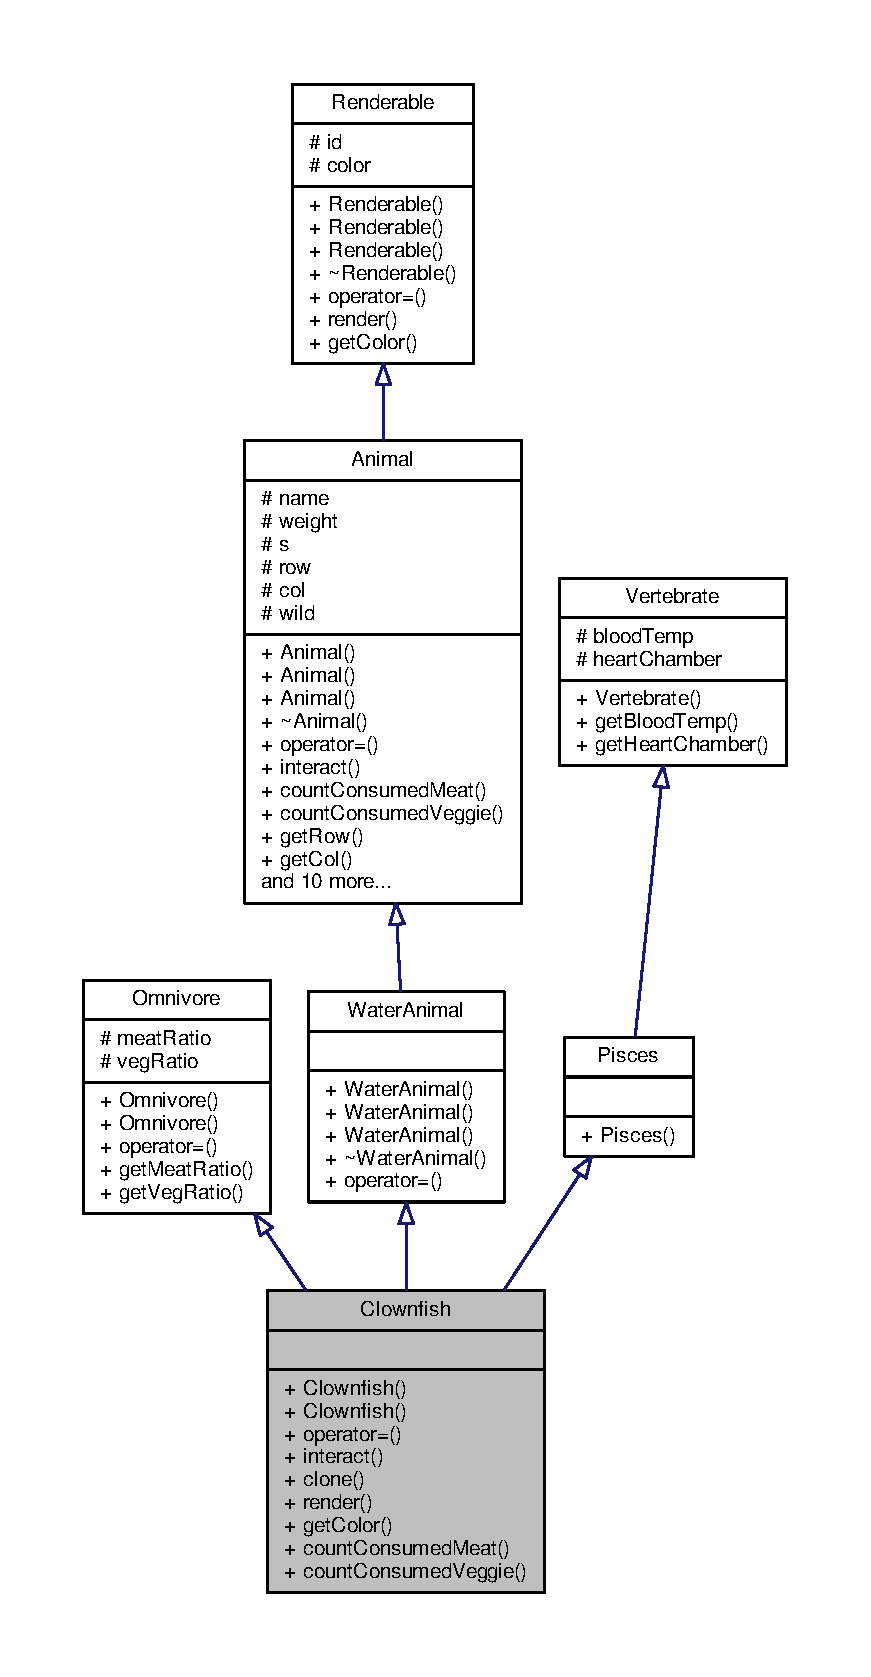
\includegraphics[height=550pt]{classClownfish__inherit__graph}
\end{center}
\end{figure}


Collaboration diagram for Clownfish\+:
\nopagebreak
\begin{figure}[H]
\begin{center}
\leavevmode
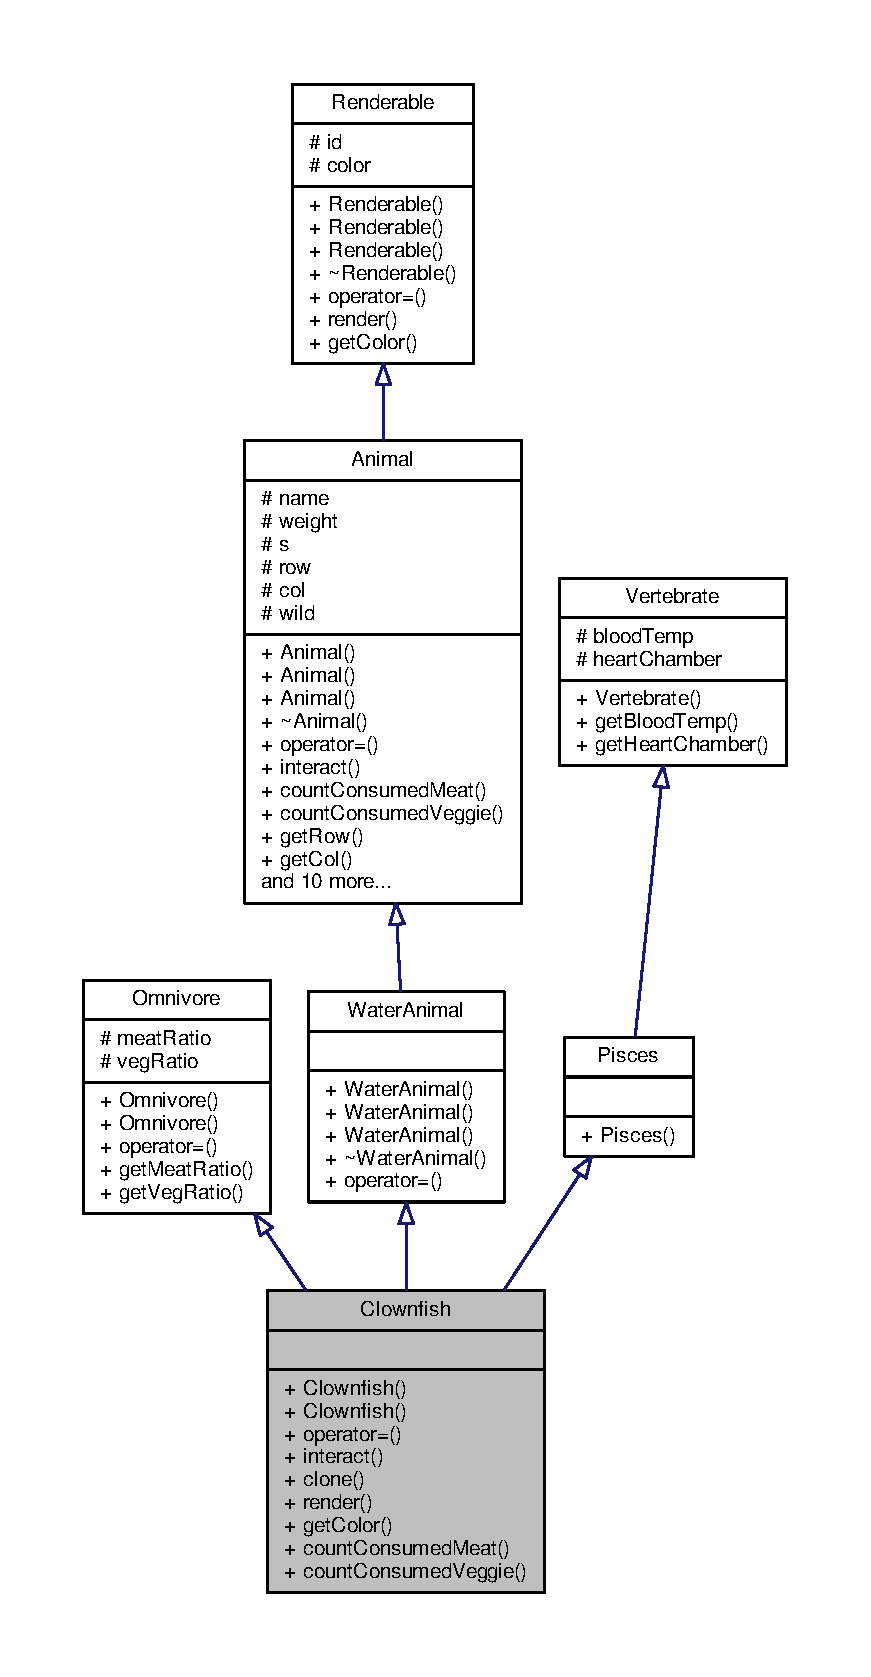
\includegraphics[height=550pt]{classClownfish__coll__graph}
\end{center}
\end{figure}
\subsection*{Public Member Functions}
\begin{DoxyCompactItemize}
\item 
\hyperlink{classClownfish_a77d6bd74aea35e208436e32b88ae67da}{Clownfish} (string \+\_\+name, double \+\_\+weight, \hyperlink{sex_8h_a2633cb393c68bb2ee8080db58fb7ba93}{Sex} \+\_\+s, int \+\_\+r, int \+\_\+c)
\begin{DoxyCompactList}\small\item\em Consructor. \end{DoxyCompactList}\item 
\hyperlink{classClownfish_ac3b7c19260b48e42dc72df3212c43685}{Clownfish} (const \hyperlink{classClownfish}{Clownfish} \&C)
\begin{DoxyCompactList}\small\item\em Copy Consructor. \end{DoxyCompactList}\item 
\hyperlink{classClownfish}{Clownfish} \& \hyperlink{classClownfish_a4d2b9efc9a7001f17bb6433c7f12a20b}{operator=} (const \hyperlink{classClownfish}{Clownfish} \&C)
\begin{DoxyCompactList}\small\item\em Operator=. Melakukan assignment pada objek. \end{DoxyCompactList}\item 
virtual void \hyperlink{classClownfish_a7c4cae7b0676de4ba55273db65d929f5}{interact} ()
\begin{DoxyCompactList}\small\item\em interact. Menampilkan interaksi hewan ke layar \end{DoxyCompactList}\item 
virtual \hyperlink{classClownfish}{Clownfish} $\ast$ \hyperlink{classClownfish_aa4ee84fc66ce7a63aa8a8d64abb26de5}{clone} () const 
\begin{DoxyCompactList}\small\item\em clone Menduplikat diri sendiri \end{DoxyCompactList}\item 
virtual char \hyperlink{classClownfish_a14417b8b2f3a9273eb9fedef9bbe9e92}{render} ()
\begin{DoxyCompactList}\small\item\em render Mengembalikan karakter id tiap hewan \end{DoxyCompactList}\item 
virtual \hyperlink{color_8h_ab87bacfdad76e61b9412d7124be44c1c}{Color} \hyperlink{classClownfish_a5c1bf33027516001957aa1e4d657ac04}{get\+Color} ()
\begin{DoxyCompactList}\small\item\em get\+Color Mengembalikan warna dari hewan \end{DoxyCompactList}\item 
virtual double \hyperlink{classClownfish_a891dd1c6ccb470273d37f4a39bfbfea8}{count\+Consumed\+Meat} ()
\begin{DoxyCompactList}\small\item\em count\+Consumed\+Meat Mengembalikan jumlah daging yang dikonsumsi \end{DoxyCompactList}\item 
virtual double \hyperlink{classClownfish_ad7c3808e5d5b7ec463e80447b505886b}{count\+Consumed\+Veggie} ()
\begin{DoxyCompactList}\small\item\em count\+Consumed\+Veggie Mengembalikan jumlah makanan tumbuhan yang dikonsumsi \end{DoxyCompactList}\end{DoxyCompactItemize}
\subsection*{Additional Inherited Members}


\subsection{Constructor \& Destructor Documentation}
\index{Clownfish@{Clownfish}!Clownfish@{Clownfish}}
\index{Clownfish@{Clownfish}!Clownfish@{Clownfish}}
\subsubsection[{\texorpdfstring{Clownfish(string \+\_\+name, double \+\_\+weight, Sex \+\_\+s, int \+\_\+r, int \+\_\+c)}{Clownfish(string _name, double _weight, Sex _s, int _r, int _c)}}]{\setlength{\rightskip}{0pt plus 5cm}Clownfish\+::\+Clownfish (
\begin{DoxyParamCaption}
\item[{string}]{\+\_\+name, }
\item[{double}]{\+\_\+weight, }
\item[{{\bf Sex}}]{\+\_\+s, }
\item[{int}]{\+\_\+r, }
\item[{int}]{\+\_\+c}
\end{DoxyParamCaption}
)}\hypertarget{classClownfish_a77d6bd74aea35e208436e32b88ae67da}{}\label{classClownfish_a77d6bd74aea35e208436e32b88ae67da}


Consructor. 


\begin{DoxyParams}{Parameters}
{\em \+\_\+name} & nama binatang \\
\hline
{\em \+\_\+weight} & berat \\
\hline
{\em \+\_\+s} & jenis kelamin \\
\hline
\end{DoxyParams}
\index{Clownfish@{Clownfish}!Clownfish@{Clownfish}}
\index{Clownfish@{Clownfish}!Clownfish@{Clownfish}}
\subsubsection[{\texorpdfstring{Clownfish(const Clownfish \&\+C)}{Clownfish(const Clownfish &C)}}]{\setlength{\rightskip}{0pt plus 5cm}Clownfish\+::\+Clownfish (
\begin{DoxyParamCaption}
\item[{const {\bf Clownfish} \&}]{C}
\end{DoxyParamCaption}
)}\hypertarget{classClownfish_ac3b7c19260b48e42dc72df3212c43685}{}\label{classClownfish_ac3b7c19260b48e42dc72df3212c43685}


Copy Consructor. 


\begin{DoxyParams}{Parameters}
{\em C} & objek yang akan disalin \\
\hline
\end{DoxyParams}


\subsection{Member Function Documentation}
\index{Clownfish@{Clownfish}!clone@{clone}}
\index{clone@{clone}!Clownfish@{Clownfish}}
\subsubsection[{\texorpdfstring{clone() const }{clone() const }}]{\setlength{\rightskip}{0pt plus 5cm}{\bf Clownfish} $\ast$ Clownfish\+::clone (
\begin{DoxyParamCaption}
{}
\end{DoxyParamCaption}
) const\hspace{0.3cm}{\ttfamily [virtual]}}\hypertarget{classClownfish_aa4ee84fc66ce7a63aa8a8d64abb26de5}{}\label{classClownfish_aa4ee84fc66ce7a63aa8a8d64abb26de5}


clone Menduplikat diri sendiri 

\begin{DoxyReturn}{Returns}
value object hasil kloning 
\end{DoxyReturn}


Implements \hyperlink{classAnimal_a1430e040ea4ff43bc453fa0ad19c308d}{Animal}.

\index{Clownfish@{Clownfish}!count\+Consumed\+Meat@{count\+Consumed\+Meat}}
\index{count\+Consumed\+Meat@{count\+Consumed\+Meat}!Clownfish@{Clownfish}}
\subsubsection[{\texorpdfstring{count\+Consumed\+Meat()}{countConsumedMeat()}}]{\setlength{\rightskip}{0pt plus 5cm}double Clownfish\+::count\+Consumed\+Meat (
\begin{DoxyParamCaption}
{}
\end{DoxyParamCaption}
)\hspace{0.3cm}{\ttfamily [virtual]}}\hypertarget{classClownfish_a891dd1c6ccb470273d37f4a39bfbfea8}{}\label{classClownfish_a891dd1c6ccb470273d37f4a39bfbfea8}


count\+Consumed\+Meat Mengembalikan jumlah daging yang dikonsumsi 

\begin{DoxyReturn}{Returns}
jumlah daging yang dikonsumsi 
\end{DoxyReturn}


Implements \hyperlink{classAnimal_a84ccc380d237650f2bf24d792627d376}{Animal}.

\index{Clownfish@{Clownfish}!count\+Consumed\+Veggie@{count\+Consumed\+Veggie}}
\index{count\+Consumed\+Veggie@{count\+Consumed\+Veggie}!Clownfish@{Clownfish}}
\subsubsection[{\texorpdfstring{count\+Consumed\+Veggie()}{countConsumedVeggie()}}]{\setlength{\rightskip}{0pt plus 5cm}double Clownfish\+::count\+Consumed\+Veggie (
\begin{DoxyParamCaption}
{}
\end{DoxyParamCaption}
)\hspace{0.3cm}{\ttfamily [virtual]}}\hypertarget{classClownfish_ad7c3808e5d5b7ec463e80447b505886b}{}\label{classClownfish_ad7c3808e5d5b7ec463e80447b505886b}


count\+Consumed\+Veggie Mengembalikan jumlah makanan tumbuhan yang dikonsumsi 

\begin{DoxyReturn}{Returns}
jumlah makanan tumbuhan yang dikonsumsi 
\end{DoxyReturn}


Implements \hyperlink{classAnimal_aaa7e4bdb7f5a10060b6dcaf09215f822}{Animal}.

\index{Clownfish@{Clownfish}!get\+Color@{get\+Color}}
\index{get\+Color@{get\+Color}!Clownfish@{Clownfish}}
\subsubsection[{\texorpdfstring{get\+Color()}{getColor()}}]{\setlength{\rightskip}{0pt plus 5cm}{\bf Color} Clownfish\+::get\+Color (
\begin{DoxyParamCaption}
{}
\end{DoxyParamCaption}
)\hspace{0.3cm}{\ttfamily [virtual]}}\hypertarget{classClownfish_a5c1bf33027516001957aa1e4d657ac04}{}\label{classClownfish_a5c1bf33027516001957aa1e4d657ac04}


get\+Color Mengembalikan warna dari hewan 

\begin{DoxyReturn}{Returns}
warna cetak hewan 
\end{DoxyReturn}


Implements \hyperlink{classRenderable_ab3bcc93b20929c6e92b64223344a73d5}{Renderable}.

\index{Clownfish@{Clownfish}!interact@{interact}}
\index{interact@{interact}!Clownfish@{Clownfish}}
\subsubsection[{\texorpdfstring{interact()}{interact()}}]{\setlength{\rightskip}{0pt plus 5cm}void Clownfish\+::interact (
\begin{DoxyParamCaption}
{}
\end{DoxyParamCaption}
)\hspace{0.3cm}{\ttfamily [virtual]}}\hypertarget{classClownfish_a7c4cae7b0676de4ba55273db65d929f5}{}\label{classClownfish_a7c4cae7b0676de4ba55273db65d929f5}


interact. Menampilkan interaksi hewan ke layar 



Implements \hyperlink{classAnimal_af47626b050b665e9a19525227d2b840f}{Animal}.

\index{Clownfish@{Clownfish}!operator=@{operator=}}
\index{operator=@{operator=}!Clownfish@{Clownfish}}
\subsubsection[{\texorpdfstring{operator=(const Clownfish \&\+C)}{operator=(const Clownfish &C)}}]{\setlength{\rightskip}{0pt plus 5cm}{\bf Clownfish} \& Clownfish\+::operator= (
\begin{DoxyParamCaption}
\item[{const {\bf Clownfish} \&}]{C}
\end{DoxyParamCaption}
)}\hypertarget{classClownfish_a4d2b9efc9a7001f17bb6433c7f12a20b}{}\label{classClownfish_a4d2b9efc9a7001f17bb6433c7f12a20b}


Operator=. Melakukan assignment pada objek. 


\begin{DoxyParams}{Parameters}
{\em C} & objek yang akan disalin \\
\hline
\end{DoxyParams}
\index{Clownfish@{Clownfish}!render@{render}}
\index{render@{render}!Clownfish@{Clownfish}}
\subsubsection[{\texorpdfstring{render()}{render()}}]{\setlength{\rightskip}{0pt plus 5cm}char Clownfish\+::render (
\begin{DoxyParamCaption}
{}
\end{DoxyParamCaption}
)\hspace{0.3cm}{\ttfamily [virtual]}}\hypertarget{classClownfish_a14417b8b2f3a9273eb9fedef9bbe9e92}{}\label{classClownfish_a14417b8b2f3a9273eb9fedef9bbe9e92}


render Mengembalikan karakter id tiap hewan 

\begin{DoxyReturn}{Returns}
karakter tiap hewan 
\end{DoxyReturn}


Implements \hyperlink{classRenderable_aafa9280e6dcfa557b3cd675221fd97b4}{Renderable}.



The documentation for this class was generated from the following files\+:\begin{DoxyCompactItemize}
\item 
src/renders/animals/\hyperlink{species_8h}{species.\+h}\item 
src/renders/animals/\hyperlink{species_8cpp}{species.\+cpp}\end{DoxyCompactItemize}

\hypertarget{classCockatoo}{}\section{Cockatoo Class Reference}
\label{classCockatoo}\index{Cockatoo@{Cockatoo}}


{\ttfamily \#include $<$species.\+h$>$}



Inheritance diagram for Cockatoo\+:
\nopagebreak
\begin{figure}[H]
\begin{center}
\leavevmode
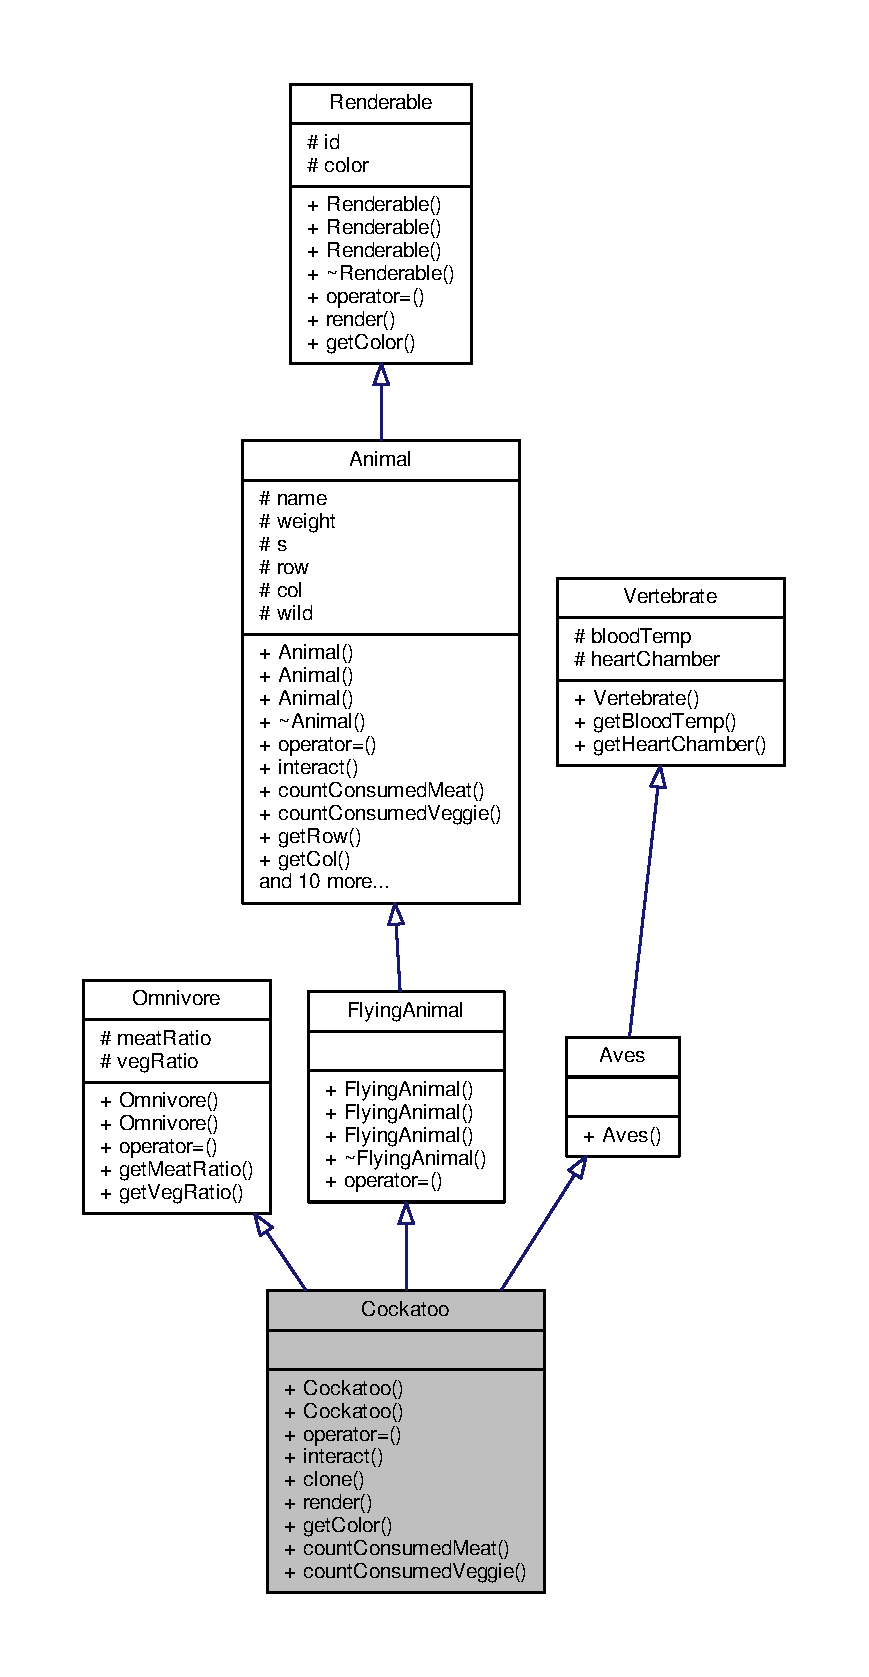
\includegraphics[height=550pt]{classCockatoo__inherit__graph}
\end{center}
\end{figure}


Collaboration diagram for Cockatoo\+:
\nopagebreak
\begin{figure}[H]
\begin{center}
\leavevmode
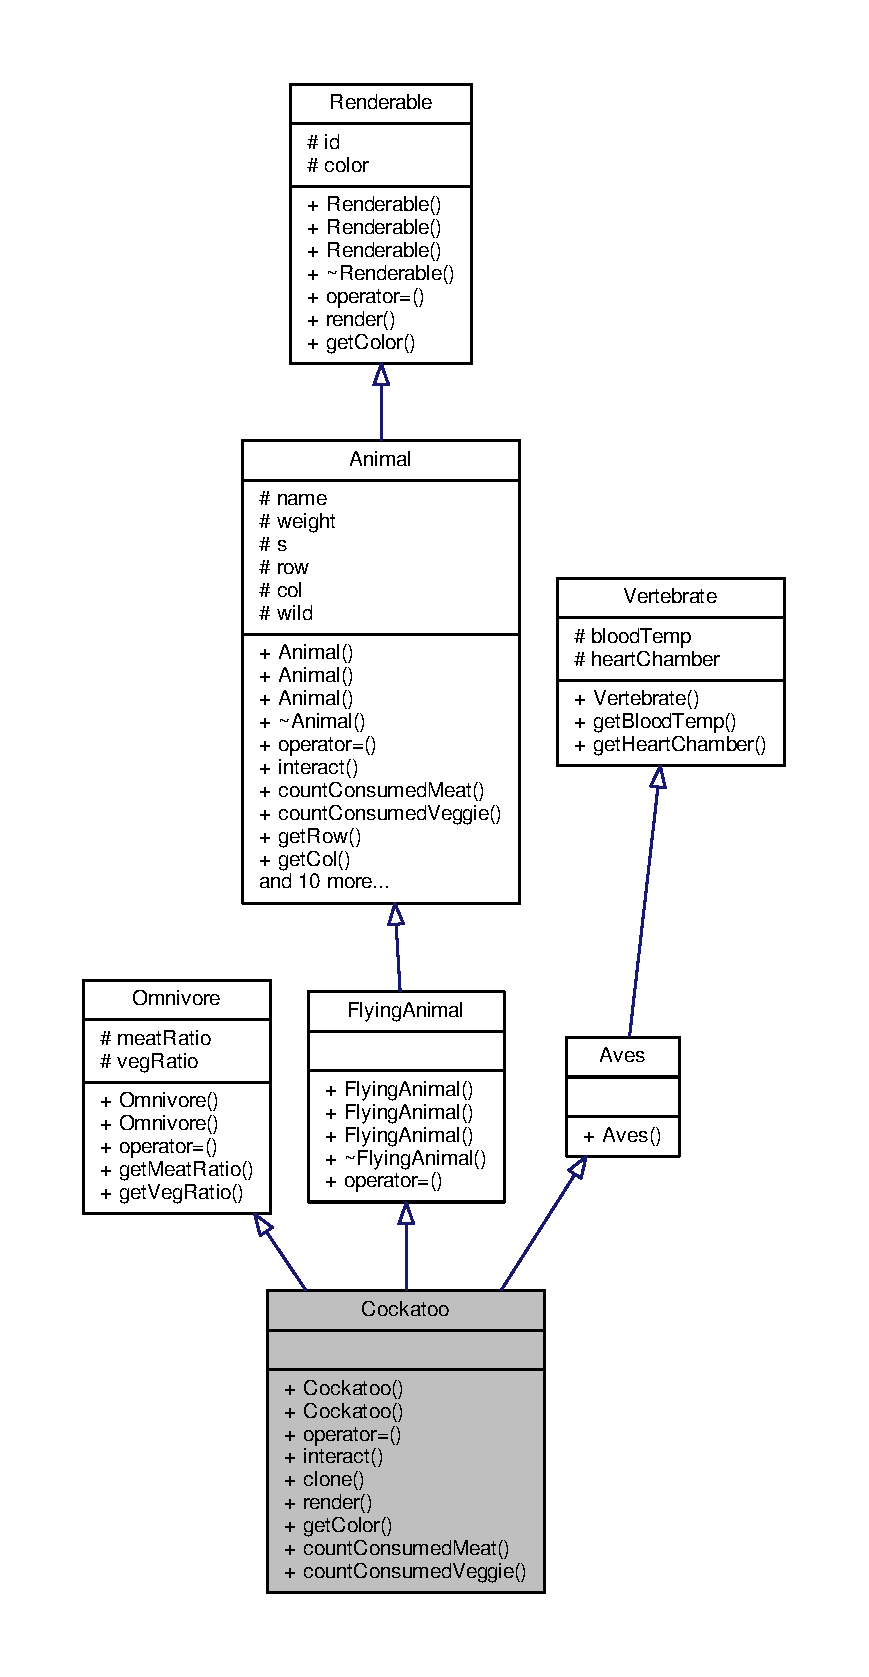
\includegraphics[height=550pt]{classCockatoo__coll__graph}
\end{center}
\end{figure}
\subsection*{Public Member Functions}
\begin{DoxyCompactItemize}
\item 
\hyperlink{classCockatoo_a5838e2eb3136afc17f69310d4c8abadc}{Cockatoo} (string \+\_\+name, double \+\_\+weight, \hyperlink{sex_8h_a2633cb393c68bb2ee8080db58fb7ba93}{Sex} \+\_\+s, int \+\_\+r, int \+\_\+c)
\begin{DoxyCompactList}\small\item\em Consructor. \end{DoxyCompactList}\item 
\hyperlink{classCockatoo_a4188365bf70f793bdeb7cca7c5405e74}{Cockatoo} (const \hyperlink{classCockatoo}{Cockatoo} \&C)
\begin{DoxyCompactList}\small\item\em Copy Consructor. \end{DoxyCompactList}\item 
\hyperlink{classCockatoo}{Cockatoo} \& \hyperlink{classCockatoo_a88f2d3fa9d377a7b6dc36172e289e0ee}{operator=} (const \hyperlink{classCockatoo}{Cockatoo} \&C)
\begin{DoxyCompactList}\small\item\em Operator=. Melakukan assignment pada objek. \end{DoxyCompactList}\item 
virtual void \hyperlink{classCockatoo_ab202d8b4fa4cafe364618a2e8c2e60ea}{interact} ()
\begin{DoxyCompactList}\small\item\em interact. Menampilkan interaksi hewan ke layar \end{DoxyCompactList}\item 
virtual \hyperlink{classCockatoo}{Cockatoo} $\ast$ \hyperlink{classCockatoo_ad679253fde6f461fa49011583d113d48}{clone} () const 
\begin{DoxyCompactList}\small\item\em clone Menduplikat diri sendiri \end{DoxyCompactList}\item 
virtual char \hyperlink{classCockatoo_af124198ac79414cd16e78ee673191585}{render} ()
\begin{DoxyCompactList}\small\item\em render Mengembalikan karakter id tiap hewan \end{DoxyCompactList}\item 
virtual \hyperlink{color_8h_ab87bacfdad76e61b9412d7124be44c1c}{Color} \hyperlink{classCockatoo_a80fc63b29d23cee2b1744499dc577612}{get\+Color} ()
\begin{DoxyCompactList}\small\item\em get\+Color Mengembalikan warna dari hewan \end{DoxyCompactList}\item 
virtual double \hyperlink{classCockatoo_a1a0ef8c860f34aee56cecd982e8d8c4b}{count\+Consumed\+Meat} ()
\begin{DoxyCompactList}\small\item\em count\+Consumed\+Meat Mengembalikan jumlah daging yang dikonsumsi \end{DoxyCompactList}\item 
virtual double \hyperlink{classCockatoo_a757745e9991110e16036d48f8468bbf5}{count\+Consumed\+Veggie} ()
\begin{DoxyCompactList}\small\item\em count\+Consumed\+Veggie Mengembalikan jumlah makanan tumbuhan yang dikonsumsi \end{DoxyCompactList}\end{DoxyCompactItemize}
\subsection*{Additional Inherited Members}


\subsection{Constructor \& Destructor Documentation}
\index{Cockatoo@{Cockatoo}!Cockatoo@{Cockatoo}}
\index{Cockatoo@{Cockatoo}!Cockatoo@{Cockatoo}}
\subsubsection[{\texorpdfstring{Cockatoo(string \+\_\+name, double \+\_\+weight, Sex \+\_\+s, int \+\_\+r, int \+\_\+c)}{Cockatoo(string _name, double _weight, Sex _s, int _r, int _c)}}]{\setlength{\rightskip}{0pt plus 5cm}Cockatoo\+::\+Cockatoo (
\begin{DoxyParamCaption}
\item[{string}]{\+\_\+name, }
\item[{double}]{\+\_\+weight, }
\item[{{\bf Sex}}]{\+\_\+s, }
\item[{int}]{\+\_\+r, }
\item[{int}]{\+\_\+c}
\end{DoxyParamCaption}
)}\hypertarget{classCockatoo_a5838e2eb3136afc17f69310d4c8abadc}{}\label{classCockatoo_a5838e2eb3136afc17f69310d4c8abadc}


Consructor. 


\begin{DoxyParams}{Parameters}
{\em \+\_\+name} & nama binatang \\
\hline
{\em \+\_\+weight} & berat \\
\hline
{\em \+\_\+s} & jenis kelamin \\
\hline
\end{DoxyParams}
\index{Cockatoo@{Cockatoo}!Cockatoo@{Cockatoo}}
\index{Cockatoo@{Cockatoo}!Cockatoo@{Cockatoo}}
\subsubsection[{\texorpdfstring{Cockatoo(const Cockatoo \&\+C)}{Cockatoo(const Cockatoo &C)}}]{\setlength{\rightskip}{0pt plus 5cm}Cockatoo\+::\+Cockatoo (
\begin{DoxyParamCaption}
\item[{const {\bf Cockatoo} \&}]{C}
\end{DoxyParamCaption}
)}\hypertarget{classCockatoo_a4188365bf70f793bdeb7cca7c5405e74}{}\label{classCockatoo_a4188365bf70f793bdeb7cca7c5405e74}


Copy Consructor. 


\begin{DoxyParams}{Parameters}
{\em C} & objek yang akan disalin \\
\hline
\end{DoxyParams}


\subsection{Member Function Documentation}
\index{Cockatoo@{Cockatoo}!clone@{clone}}
\index{clone@{clone}!Cockatoo@{Cockatoo}}
\subsubsection[{\texorpdfstring{clone() const }{clone() const }}]{\setlength{\rightskip}{0pt plus 5cm}{\bf Cockatoo} $\ast$ Cockatoo\+::clone (
\begin{DoxyParamCaption}
{}
\end{DoxyParamCaption}
) const\hspace{0.3cm}{\ttfamily [virtual]}}\hypertarget{classCockatoo_ad679253fde6f461fa49011583d113d48}{}\label{classCockatoo_ad679253fde6f461fa49011583d113d48}


clone Menduplikat diri sendiri 

\begin{DoxyReturn}{Returns}
value object hasil kloning 
\end{DoxyReturn}


Implements \hyperlink{classAnimal_a1430e040ea4ff43bc453fa0ad19c308d}{Animal}.

\index{Cockatoo@{Cockatoo}!count\+Consumed\+Meat@{count\+Consumed\+Meat}}
\index{count\+Consumed\+Meat@{count\+Consumed\+Meat}!Cockatoo@{Cockatoo}}
\subsubsection[{\texorpdfstring{count\+Consumed\+Meat()}{countConsumedMeat()}}]{\setlength{\rightskip}{0pt plus 5cm}double Cockatoo\+::count\+Consumed\+Meat (
\begin{DoxyParamCaption}
{}
\end{DoxyParamCaption}
)\hspace{0.3cm}{\ttfamily [virtual]}}\hypertarget{classCockatoo_a1a0ef8c860f34aee56cecd982e8d8c4b}{}\label{classCockatoo_a1a0ef8c860f34aee56cecd982e8d8c4b}


count\+Consumed\+Meat Mengembalikan jumlah daging yang dikonsumsi 

\begin{DoxyReturn}{Returns}
jumlah daging yang dikonsumsi 
\end{DoxyReturn}


Implements \hyperlink{classAnimal_a84ccc380d237650f2bf24d792627d376}{Animal}.

\index{Cockatoo@{Cockatoo}!count\+Consumed\+Veggie@{count\+Consumed\+Veggie}}
\index{count\+Consumed\+Veggie@{count\+Consumed\+Veggie}!Cockatoo@{Cockatoo}}
\subsubsection[{\texorpdfstring{count\+Consumed\+Veggie()}{countConsumedVeggie()}}]{\setlength{\rightskip}{0pt plus 5cm}double Cockatoo\+::count\+Consumed\+Veggie (
\begin{DoxyParamCaption}
{}
\end{DoxyParamCaption}
)\hspace{0.3cm}{\ttfamily [virtual]}}\hypertarget{classCockatoo_a757745e9991110e16036d48f8468bbf5}{}\label{classCockatoo_a757745e9991110e16036d48f8468bbf5}


count\+Consumed\+Veggie Mengembalikan jumlah makanan tumbuhan yang dikonsumsi 

\begin{DoxyReturn}{Returns}
jumlah makanan tumbuhan yang dikonsumsi 
\end{DoxyReturn}


Implements \hyperlink{classAnimal_aaa7e4bdb7f5a10060b6dcaf09215f822}{Animal}.

\index{Cockatoo@{Cockatoo}!get\+Color@{get\+Color}}
\index{get\+Color@{get\+Color}!Cockatoo@{Cockatoo}}
\subsubsection[{\texorpdfstring{get\+Color()}{getColor()}}]{\setlength{\rightskip}{0pt plus 5cm}{\bf Color} Cockatoo\+::get\+Color (
\begin{DoxyParamCaption}
{}
\end{DoxyParamCaption}
)\hspace{0.3cm}{\ttfamily [virtual]}}\hypertarget{classCockatoo_a80fc63b29d23cee2b1744499dc577612}{}\label{classCockatoo_a80fc63b29d23cee2b1744499dc577612}


get\+Color Mengembalikan warna dari hewan 

\begin{DoxyReturn}{Returns}
warna cetak hewan 
\end{DoxyReturn}


Implements \hyperlink{classRenderable_ab3bcc93b20929c6e92b64223344a73d5}{Renderable}.

\index{Cockatoo@{Cockatoo}!interact@{interact}}
\index{interact@{interact}!Cockatoo@{Cockatoo}}
\subsubsection[{\texorpdfstring{interact()}{interact()}}]{\setlength{\rightskip}{0pt plus 5cm}void Cockatoo\+::interact (
\begin{DoxyParamCaption}
{}
\end{DoxyParamCaption}
)\hspace{0.3cm}{\ttfamily [virtual]}}\hypertarget{classCockatoo_ab202d8b4fa4cafe364618a2e8c2e60ea}{}\label{classCockatoo_ab202d8b4fa4cafe364618a2e8c2e60ea}


interact. Menampilkan interaksi hewan ke layar 



Implements \hyperlink{classAnimal_af47626b050b665e9a19525227d2b840f}{Animal}.

\index{Cockatoo@{Cockatoo}!operator=@{operator=}}
\index{operator=@{operator=}!Cockatoo@{Cockatoo}}
\subsubsection[{\texorpdfstring{operator=(const Cockatoo \&\+C)}{operator=(const Cockatoo &C)}}]{\setlength{\rightskip}{0pt plus 5cm}{\bf Cockatoo} \& Cockatoo\+::operator= (
\begin{DoxyParamCaption}
\item[{const {\bf Cockatoo} \&}]{C}
\end{DoxyParamCaption}
)}\hypertarget{classCockatoo_a88f2d3fa9d377a7b6dc36172e289e0ee}{}\label{classCockatoo_a88f2d3fa9d377a7b6dc36172e289e0ee}


Operator=. Melakukan assignment pada objek. 


\begin{DoxyParams}{Parameters}
{\em C} & objek yang akan disalin \\
\hline
\end{DoxyParams}
\index{Cockatoo@{Cockatoo}!render@{render}}
\index{render@{render}!Cockatoo@{Cockatoo}}
\subsubsection[{\texorpdfstring{render()}{render()}}]{\setlength{\rightskip}{0pt plus 5cm}char Cockatoo\+::render (
\begin{DoxyParamCaption}
{}
\end{DoxyParamCaption}
)\hspace{0.3cm}{\ttfamily [virtual]}}\hypertarget{classCockatoo_af124198ac79414cd16e78ee673191585}{}\label{classCockatoo_af124198ac79414cd16e78ee673191585}


render Mengembalikan karakter id tiap hewan 

\begin{DoxyReturn}{Returns}
karakter tiap hewan 
\end{DoxyReturn}


Implements \hyperlink{classRenderable_aafa9280e6dcfa557b3cd675221fd97b4}{Renderable}.



The documentation for this class was generated from the following files\+:\begin{DoxyCompactItemize}
\item 
src/renders/animals/\hyperlink{species_8h}{species.\+h}\item 
src/renders/animals/\hyperlink{species_8cpp}{species.\+cpp}\end{DoxyCompactItemize}

\hypertarget{classDolphin}{}\section{Dolphin Class Reference}
\label{classDolphin}\index{Dolphin@{Dolphin}}


{\ttfamily \#include $<$species.\+h$>$}



Inheritance diagram for Dolphin\+:
\nopagebreak
\begin{figure}[H]
\begin{center}
\leavevmode
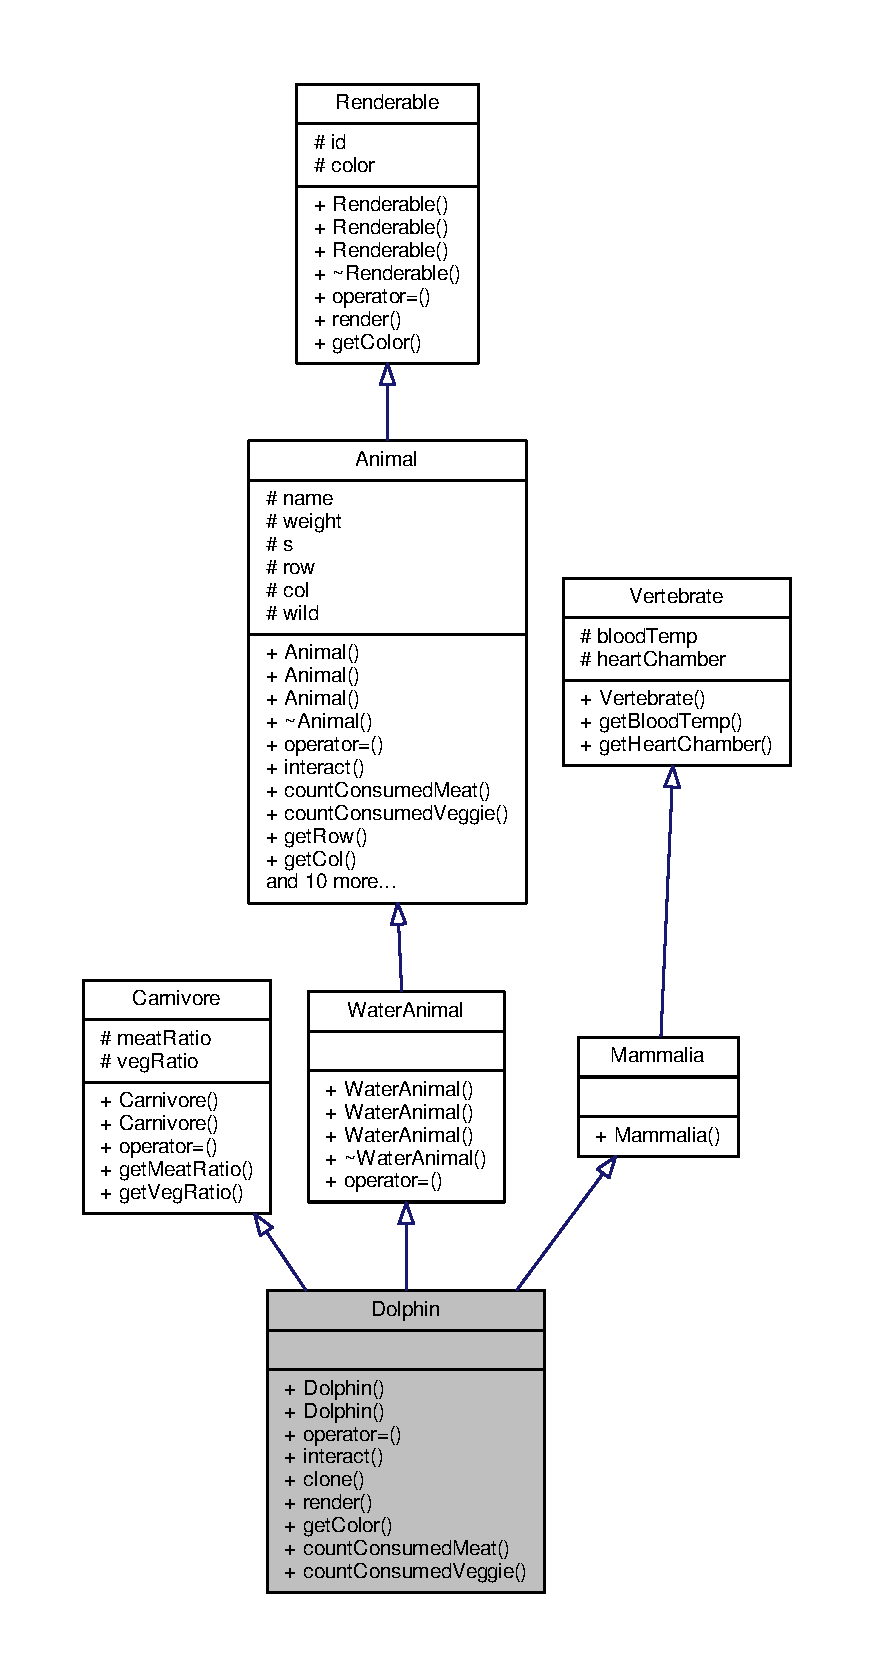
\includegraphics[height=550pt]{classDolphin__inherit__graph}
\end{center}
\end{figure}


Collaboration diagram for Dolphin\+:
\nopagebreak
\begin{figure}[H]
\begin{center}
\leavevmode
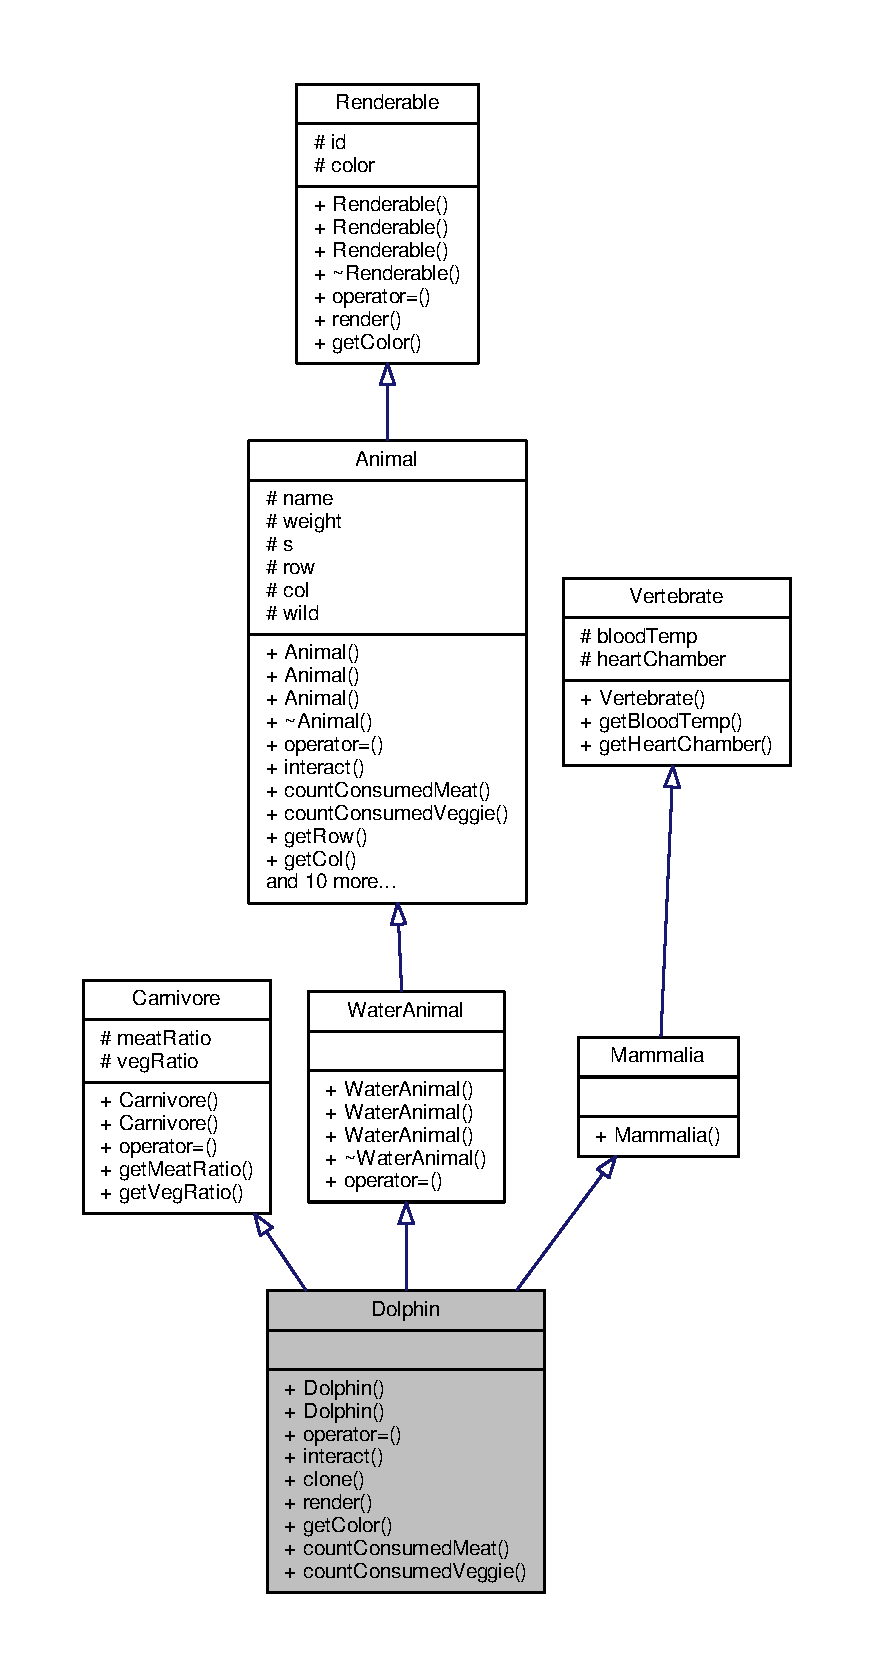
\includegraphics[height=550pt]{classDolphin__coll__graph}
\end{center}
\end{figure}
\subsection*{Public Member Functions}
\begin{DoxyCompactItemize}
\item 
\hyperlink{classDolphin_a8f376b2e32eb805b23f5d5f3048762d0}{Dolphin} (string \+\_\+name, double \+\_\+weight, \hyperlink{sex_8h_a2633cb393c68bb2ee8080db58fb7ba93}{Sex} \+\_\+s, int \+\_\+r, int \+\_\+c)
\begin{DoxyCompactList}\small\item\em Consructor. \end{DoxyCompactList}\item 
\hyperlink{classDolphin_a5b947f871569362a63f5338fc10b0a11}{Dolphin} (const \hyperlink{classDolphin}{Dolphin} \&D)
\begin{DoxyCompactList}\small\item\em Copy Consructor. \end{DoxyCompactList}\item 
\hyperlink{classDolphin}{Dolphin} \& \hyperlink{classDolphin_a62d8e42dd19d6221bac770ae0710bdd7}{operator=} (const \hyperlink{classDolphin}{Dolphin} \&D)
\begin{DoxyCompactList}\small\item\em Operator=. Melakukan assignment pada objek. \end{DoxyCompactList}\item 
virtual void \hyperlink{classDolphin_a6d5b202824f7f12e6286b2b09489c342}{interact} ()
\begin{DoxyCompactList}\small\item\em interact. Menampilkan interaksi hewan ke layar \end{DoxyCompactList}\item 
virtual \hyperlink{classDolphin}{Dolphin} $\ast$ \hyperlink{classDolphin_a77c541ea19646ec22a5461cb9788ccb6}{clone} () const 
\begin{DoxyCompactList}\small\item\em clone Menduplikat diri sendiri \end{DoxyCompactList}\item 
virtual char \hyperlink{classDolphin_aa7c379b5806f594e54021429b99141a9}{render} ()
\begin{DoxyCompactList}\small\item\em render Mengembalikan karakter id tiap hewan \end{DoxyCompactList}\item 
virtual \hyperlink{color_8h_ab87bacfdad76e61b9412d7124be44c1c}{Color} \hyperlink{classDolphin_a425bde02c5be7ddd955380b99249469e}{get\+Color} ()
\begin{DoxyCompactList}\small\item\em get\+Color Mengembalikan warna dari hewan \end{DoxyCompactList}\item 
virtual double \hyperlink{classDolphin_a6c53ee214a0092e13417645b16387596}{count\+Consumed\+Meat} ()
\begin{DoxyCompactList}\small\item\em count\+Consumed\+Meat Mengembalikan jumlah daging yang dikonsumsi \end{DoxyCompactList}\item 
virtual double \hyperlink{classDolphin_a528ae87e039dcb252d90815e37535eb9}{count\+Consumed\+Veggie} ()
\begin{DoxyCompactList}\small\item\em count\+Consumed\+Veggie Mengembalikan jumlah makanan tumbuhan yang dikonsumsi \end{DoxyCompactList}\end{DoxyCompactItemize}
\subsection*{Additional Inherited Members}


\subsection{Constructor \& Destructor Documentation}
\index{Dolphin@{Dolphin}!Dolphin@{Dolphin}}
\index{Dolphin@{Dolphin}!Dolphin@{Dolphin}}
\subsubsection[{\texorpdfstring{Dolphin(string \+\_\+name, double \+\_\+weight, Sex \+\_\+s, int \+\_\+r, int \+\_\+c)}{Dolphin(string _name, double _weight, Sex _s, int _r, int _c)}}]{\setlength{\rightskip}{0pt plus 5cm}Dolphin\+::\+Dolphin (
\begin{DoxyParamCaption}
\item[{string}]{\+\_\+name, }
\item[{double}]{\+\_\+weight, }
\item[{{\bf Sex}}]{\+\_\+s, }
\item[{int}]{\+\_\+r, }
\item[{int}]{\+\_\+c}
\end{DoxyParamCaption}
)}\hypertarget{classDolphin_a8f376b2e32eb805b23f5d5f3048762d0}{}\label{classDolphin_a8f376b2e32eb805b23f5d5f3048762d0}


Consructor. 


\begin{DoxyParams}{Parameters}
{\em \+\_\+name} & nama binatang \\
\hline
{\em \+\_\+weight} & berat \\
\hline
{\em \+\_\+s} & jenis kelamin \\
\hline
\end{DoxyParams}
\index{Dolphin@{Dolphin}!Dolphin@{Dolphin}}
\index{Dolphin@{Dolphin}!Dolphin@{Dolphin}}
\subsubsection[{\texorpdfstring{Dolphin(const Dolphin \&\+D)}{Dolphin(const Dolphin &D)}}]{\setlength{\rightskip}{0pt plus 5cm}Dolphin\+::\+Dolphin (
\begin{DoxyParamCaption}
\item[{const {\bf Dolphin} \&}]{D}
\end{DoxyParamCaption}
)}\hypertarget{classDolphin_a5b947f871569362a63f5338fc10b0a11}{}\label{classDolphin_a5b947f871569362a63f5338fc10b0a11}


Copy Consructor. 


\begin{DoxyParams}{Parameters}
{\em D} & objek yang akan disalin \\
\hline
\end{DoxyParams}


\subsection{Member Function Documentation}
\index{Dolphin@{Dolphin}!clone@{clone}}
\index{clone@{clone}!Dolphin@{Dolphin}}
\subsubsection[{\texorpdfstring{clone() const }{clone() const }}]{\setlength{\rightskip}{0pt plus 5cm}{\bf Dolphin} $\ast$ Dolphin\+::clone (
\begin{DoxyParamCaption}
{}
\end{DoxyParamCaption}
) const\hspace{0.3cm}{\ttfamily [virtual]}}\hypertarget{classDolphin_a77c541ea19646ec22a5461cb9788ccb6}{}\label{classDolphin_a77c541ea19646ec22a5461cb9788ccb6}


clone Menduplikat diri sendiri 

\begin{DoxyReturn}{Returns}
value object hasil kloning 
\end{DoxyReturn}


Implements \hyperlink{classAnimal_a1430e040ea4ff43bc453fa0ad19c308d}{Animal}.

\index{Dolphin@{Dolphin}!count\+Consumed\+Meat@{count\+Consumed\+Meat}}
\index{count\+Consumed\+Meat@{count\+Consumed\+Meat}!Dolphin@{Dolphin}}
\subsubsection[{\texorpdfstring{count\+Consumed\+Meat()}{countConsumedMeat()}}]{\setlength{\rightskip}{0pt plus 5cm}double Dolphin\+::count\+Consumed\+Meat (
\begin{DoxyParamCaption}
{}
\end{DoxyParamCaption}
)\hspace{0.3cm}{\ttfamily [virtual]}}\hypertarget{classDolphin_a6c53ee214a0092e13417645b16387596}{}\label{classDolphin_a6c53ee214a0092e13417645b16387596}


count\+Consumed\+Meat Mengembalikan jumlah daging yang dikonsumsi 

\begin{DoxyReturn}{Returns}
jumlah daging yang dikonsumsi 
\end{DoxyReturn}


Implements \hyperlink{classAnimal_a84ccc380d237650f2bf24d792627d376}{Animal}.

\index{Dolphin@{Dolphin}!count\+Consumed\+Veggie@{count\+Consumed\+Veggie}}
\index{count\+Consumed\+Veggie@{count\+Consumed\+Veggie}!Dolphin@{Dolphin}}
\subsubsection[{\texorpdfstring{count\+Consumed\+Veggie()}{countConsumedVeggie()}}]{\setlength{\rightskip}{0pt plus 5cm}double Dolphin\+::count\+Consumed\+Veggie (
\begin{DoxyParamCaption}
{}
\end{DoxyParamCaption}
)\hspace{0.3cm}{\ttfamily [virtual]}}\hypertarget{classDolphin_a528ae87e039dcb252d90815e37535eb9}{}\label{classDolphin_a528ae87e039dcb252d90815e37535eb9}


count\+Consumed\+Veggie Mengembalikan jumlah makanan tumbuhan yang dikonsumsi 

\begin{DoxyReturn}{Returns}
jumlah makanan tumbuhan yang dikonsumsi 
\end{DoxyReturn}


Implements \hyperlink{classAnimal_aaa7e4bdb7f5a10060b6dcaf09215f822}{Animal}.

\index{Dolphin@{Dolphin}!get\+Color@{get\+Color}}
\index{get\+Color@{get\+Color}!Dolphin@{Dolphin}}
\subsubsection[{\texorpdfstring{get\+Color()}{getColor()}}]{\setlength{\rightskip}{0pt plus 5cm}{\bf Color} Dolphin\+::get\+Color (
\begin{DoxyParamCaption}
{}
\end{DoxyParamCaption}
)\hspace{0.3cm}{\ttfamily [virtual]}}\hypertarget{classDolphin_a425bde02c5be7ddd955380b99249469e}{}\label{classDolphin_a425bde02c5be7ddd955380b99249469e}


get\+Color Mengembalikan warna dari hewan 

\begin{DoxyReturn}{Returns}
warna cetak hewan 
\end{DoxyReturn}


Implements \hyperlink{classRenderable_ab3bcc93b20929c6e92b64223344a73d5}{Renderable}.

\index{Dolphin@{Dolphin}!interact@{interact}}
\index{interact@{interact}!Dolphin@{Dolphin}}
\subsubsection[{\texorpdfstring{interact()}{interact()}}]{\setlength{\rightskip}{0pt plus 5cm}void Dolphin\+::interact (
\begin{DoxyParamCaption}
{}
\end{DoxyParamCaption}
)\hspace{0.3cm}{\ttfamily [virtual]}}\hypertarget{classDolphin_a6d5b202824f7f12e6286b2b09489c342}{}\label{classDolphin_a6d5b202824f7f12e6286b2b09489c342}


interact. Menampilkan interaksi hewan ke layar 



Implements \hyperlink{classAnimal_af47626b050b665e9a19525227d2b840f}{Animal}.

\index{Dolphin@{Dolphin}!operator=@{operator=}}
\index{operator=@{operator=}!Dolphin@{Dolphin}}
\subsubsection[{\texorpdfstring{operator=(const Dolphin \&\+D)}{operator=(const Dolphin &D)}}]{\setlength{\rightskip}{0pt plus 5cm}{\bf Dolphin} \& Dolphin\+::operator= (
\begin{DoxyParamCaption}
\item[{const {\bf Dolphin} \&}]{D}
\end{DoxyParamCaption}
)}\hypertarget{classDolphin_a62d8e42dd19d6221bac770ae0710bdd7}{}\label{classDolphin_a62d8e42dd19d6221bac770ae0710bdd7}


Operator=. Melakukan assignment pada objek. 


\begin{DoxyParams}{Parameters}
{\em D} & objek yang akan disalin \\
\hline
\end{DoxyParams}
\index{Dolphin@{Dolphin}!render@{render}}
\index{render@{render}!Dolphin@{Dolphin}}
\subsubsection[{\texorpdfstring{render()}{render()}}]{\setlength{\rightskip}{0pt plus 5cm}char Dolphin\+::render (
\begin{DoxyParamCaption}
{}
\end{DoxyParamCaption}
)\hspace{0.3cm}{\ttfamily [virtual]}}\hypertarget{classDolphin_aa7c379b5806f594e54021429b99141a9}{}\label{classDolphin_aa7c379b5806f594e54021429b99141a9}


render Mengembalikan karakter id tiap hewan 

\begin{DoxyReturn}{Returns}
karakter tiap hewan 
\end{DoxyReturn}


Implements \hyperlink{classRenderable_aafa9280e6dcfa557b3cd675221fd97b4}{Renderable}.



The documentation for this class was generated from the following files\+:\begin{DoxyCompactItemize}
\item 
src/renders/animals/\hyperlink{species_8h}{species.\+h}\item 
src/renders/animals/\hyperlink{species_8cpp}{species.\+cpp}\end{DoxyCompactItemize}

\hypertarget{classDriver}{}\section{Driver Class Reference}
\label{classDriver}\index{Driver@{Driver}}


{\ttfamily \#include $<$driver.\+h$>$}



Collaboration diagram for Driver\+:
\nopagebreak
\begin{figure}[H]
\begin{center}
\leavevmode
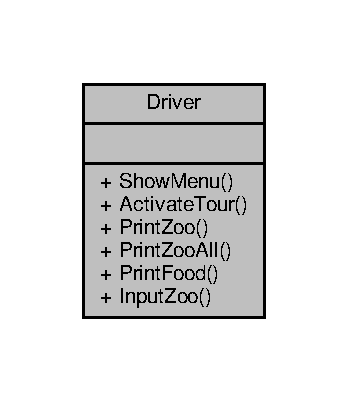
\includegraphics[width=167pt]{classDriver__coll__graph}
\end{center}
\end{figure}
\subsection*{Static Public Member Functions}
\begin{DoxyCompactItemize}
\item 
static void \hyperlink{classDriver_a3cbec9699953cf65b23eae3ced1338bb}{Show\+Menu} ()
\begin{DoxyCompactList}\small\item\em Menampilkan menu. Mencetak menu tampilan utama bagi pengguna. \end{DoxyCompactList}\item 
static void \hyperlink{classDriver_ab43c2330f27a0391bc39be75d348562a}{Activate\+Tour} (\hyperlink{classZoo}{Zoo} \&Z)
\begin{DoxyCompactList}\small\item\em Aktivasi Tour Memulai Tour kebun binatang. \end{DoxyCompactList}\item 
static void \hyperlink{classDriver_a631e22aab57fd7ac4200bccd6fbcb221}{Print\+Zoo} (\hyperlink{classZoo}{Zoo} \&Z, int x1, int y1, int x2, int y2)
\begin{DoxyCompactList}\small\item\em Menampilkan kebun binatang. Memanggil fungsi display dari zoo untuk menampilkan zoo. \end{DoxyCompactList}\item 
static void \hyperlink{classDriver_a73f290d28efdb356bbf0355cf99e3b1f}{Print\+Zoo\+All} (\hyperlink{classZoo}{Zoo} \&Z)
\begin{DoxyCompactList}\small\item\em Menampilkan kebun binatang. Memanggil fungsi display dari zoo untuk menampilkan seluruh zoo. \end{DoxyCompactList}\item 
static void \hyperlink{classDriver_aa7c89da61c5d5810a71048e6a49024e4}{Print\+Food} (\hyperlink{classZoo}{Zoo} \&Z)
\begin{DoxyCompactList}\small\item\em Menampilkan makanan yang dikonsumsi hewan di kebun Z. \end{DoxyCompactList}\item 
static void \hyperlink{classDriver_aff036df2efc67fbf6c20a1dcd3547855}{Input\+Zoo} (\hyperlink{classZoo}{Zoo} \&Z)
\begin{DoxyCompactList}\small\item\em Membaca \hyperlink{classZoo}{Zoo} Z dari File Memanfaatkan method read\+All pada kelas \hyperlink{classZoo}{Zoo}. \end{DoxyCompactList}\end{DoxyCompactItemize}


\subsection{Detailed Description}
Kelas yang menjalankan kebun binatang virtual 

\subsection{Member Function Documentation}
\index{Driver@{Driver}!Activate\+Tour@{Activate\+Tour}}
\index{Activate\+Tour@{Activate\+Tour}!Driver@{Driver}}
\subsubsection[{\texorpdfstring{Activate\+Tour(\+Zoo \&\+Z)}{ActivateTour(Zoo &Z)}}]{\setlength{\rightskip}{0pt plus 5cm}void Driver\+::\+Activate\+Tour (
\begin{DoxyParamCaption}
\item[{{\bf Zoo} \&}]{Z}
\end{DoxyParamCaption}
)\hspace{0.3cm}{\ttfamily [static]}}\hypertarget{classDriver_ab43c2330f27a0391bc39be75d348562a}{}\label{classDriver_ab43c2330f27a0391bc39be75d348562a}


Aktivasi Tour Memulai Tour kebun binatang. 


\begin{DoxyParams}{Parameters}
{\em Z} & kebun binatang yang memulai tour \\
\hline
\end{DoxyParams}
\index{Driver@{Driver}!Input\+Zoo@{Input\+Zoo}}
\index{Input\+Zoo@{Input\+Zoo}!Driver@{Driver}}
\subsubsection[{\texorpdfstring{Input\+Zoo(\+Zoo \&\+Z)}{InputZoo(Zoo &Z)}}]{\setlength{\rightskip}{0pt plus 5cm}void Driver\+::\+Input\+Zoo (
\begin{DoxyParamCaption}
\item[{{\bf Zoo} \&}]{Z}
\end{DoxyParamCaption}
)\hspace{0.3cm}{\ttfamily [static]}}\hypertarget{classDriver_aff036df2efc67fbf6c20a1dcd3547855}{}\label{classDriver_aff036df2efc67fbf6c20a1dcd3547855}


Membaca \hyperlink{classZoo}{Zoo} Z dari File Memanfaatkan method read\+All pada kelas \hyperlink{classZoo}{Zoo}. 


\begin{DoxyParams}{Parameters}
{\em Z} & kebun binatang yang ingin dibaca dari file. \\
\hline
\end{DoxyParams}
\index{Driver@{Driver}!Print\+Food@{Print\+Food}}
\index{Print\+Food@{Print\+Food}!Driver@{Driver}}
\subsubsection[{\texorpdfstring{Print\+Food(\+Zoo \&\+Z)}{PrintFood(Zoo &Z)}}]{\setlength{\rightskip}{0pt plus 5cm}void Driver\+::\+Print\+Food (
\begin{DoxyParamCaption}
\item[{{\bf Zoo} \&}]{Z}
\end{DoxyParamCaption}
)\hspace{0.3cm}{\ttfamily [static]}}\hypertarget{classDriver_aa7c89da61c5d5810a71048e6a49024e4}{}\label{classDriver_aa7c89da61c5d5810a71048e6a49024e4}


Menampilkan makanan yang dikonsumsi hewan di kebun Z. 


\begin{DoxyParams}{Parameters}
{\em Z} & kebun binatang yang ingin dihitung makanan yang dikonsumsinya. \\
\hline
\end{DoxyParams}
\index{Driver@{Driver}!Print\+Zoo@{Print\+Zoo}}
\index{Print\+Zoo@{Print\+Zoo}!Driver@{Driver}}
\subsubsection[{\texorpdfstring{Print\+Zoo(\+Zoo \&\+Z, int x1, int y1, int x2, int y2)}{PrintZoo(Zoo &Z, int x1, int y1, int x2, int y2)}}]{\setlength{\rightskip}{0pt plus 5cm}void Driver\+::\+Print\+Zoo (
\begin{DoxyParamCaption}
\item[{{\bf Zoo} \&}]{Z, }
\item[{int}]{x1, }
\item[{int}]{y1, }
\item[{int}]{x2, }
\item[{int}]{y2}
\end{DoxyParamCaption}
)\hspace{0.3cm}{\ttfamily [static]}}\hypertarget{classDriver_a631e22aab57fd7ac4200bccd6fbcb221}{}\label{classDriver_a631e22aab57fd7ac4200bccd6fbcb221}


Menampilkan kebun binatang. Memanggil fungsi display dari zoo untuk menampilkan zoo. 


\begin{DoxyParams}{Parameters}
{\em Z} & kebun binatang yang dicetak \\
\hline
{\em x1} & indeks baris ujung kiri \\
\hline
{\em y1} & indeks kolom ujung kiri \\
\hline
{\em x2} & indeks baris ujung kanan \\
\hline
{\em y2} & indeks kolom ujung kanan \\
\hline
\end{DoxyParams}
\index{Driver@{Driver}!Print\+Zoo\+All@{Print\+Zoo\+All}}
\index{Print\+Zoo\+All@{Print\+Zoo\+All}!Driver@{Driver}}
\subsubsection[{\texorpdfstring{Print\+Zoo\+All(\+Zoo \&\+Z)}{PrintZooAll(Zoo &Z)}}]{\setlength{\rightskip}{0pt plus 5cm}void Driver\+::\+Print\+Zoo\+All (
\begin{DoxyParamCaption}
\item[{{\bf Zoo} \&}]{Z}
\end{DoxyParamCaption}
)\hspace{0.3cm}{\ttfamily [static]}}\hypertarget{classDriver_a73f290d28efdb356bbf0355cf99e3b1f}{}\label{classDriver_a73f290d28efdb356bbf0355cf99e3b1f}


Menampilkan kebun binatang. Memanggil fungsi display dari zoo untuk menampilkan seluruh zoo. 


\begin{DoxyParams}{Parameters}
{\em Z} & kebun binatang yang dicetak \\
\hline
\end{DoxyParams}
\index{Driver@{Driver}!Show\+Menu@{Show\+Menu}}
\index{Show\+Menu@{Show\+Menu}!Driver@{Driver}}
\subsubsection[{\texorpdfstring{Show\+Menu()}{ShowMenu()}}]{\setlength{\rightskip}{0pt plus 5cm}void Driver\+::\+Show\+Menu (
\begin{DoxyParamCaption}
{}
\end{DoxyParamCaption}
)\hspace{0.3cm}{\ttfamily [static]}}\hypertarget{classDriver_a3cbec9699953cf65b23eae3ced1338bb}{}\label{classDriver_a3cbec9699953cf65b23eae3ced1338bb}


Menampilkan menu. Mencetak menu tampilan utama bagi pengguna. 



The documentation for this class was generated from the following files\+:\begin{DoxyCompactItemize}
\item 
src/driver/\hyperlink{driver_8h}{driver.\+h}\item 
src/driver/\hyperlink{driver_8cpp}{driver.\+cpp}\end{DoxyCompactItemize}

\hypertarget{classEagle}{}\section{Eagle Class Reference}
\label{classEagle}\index{Eagle@{Eagle}}


{\ttfamily \#include $<$species.\+h$>$}



Inheritance diagram for Eagle\+:
\nopagebreak
\begin{figure}[H]
\begin{center}
\leavevmode
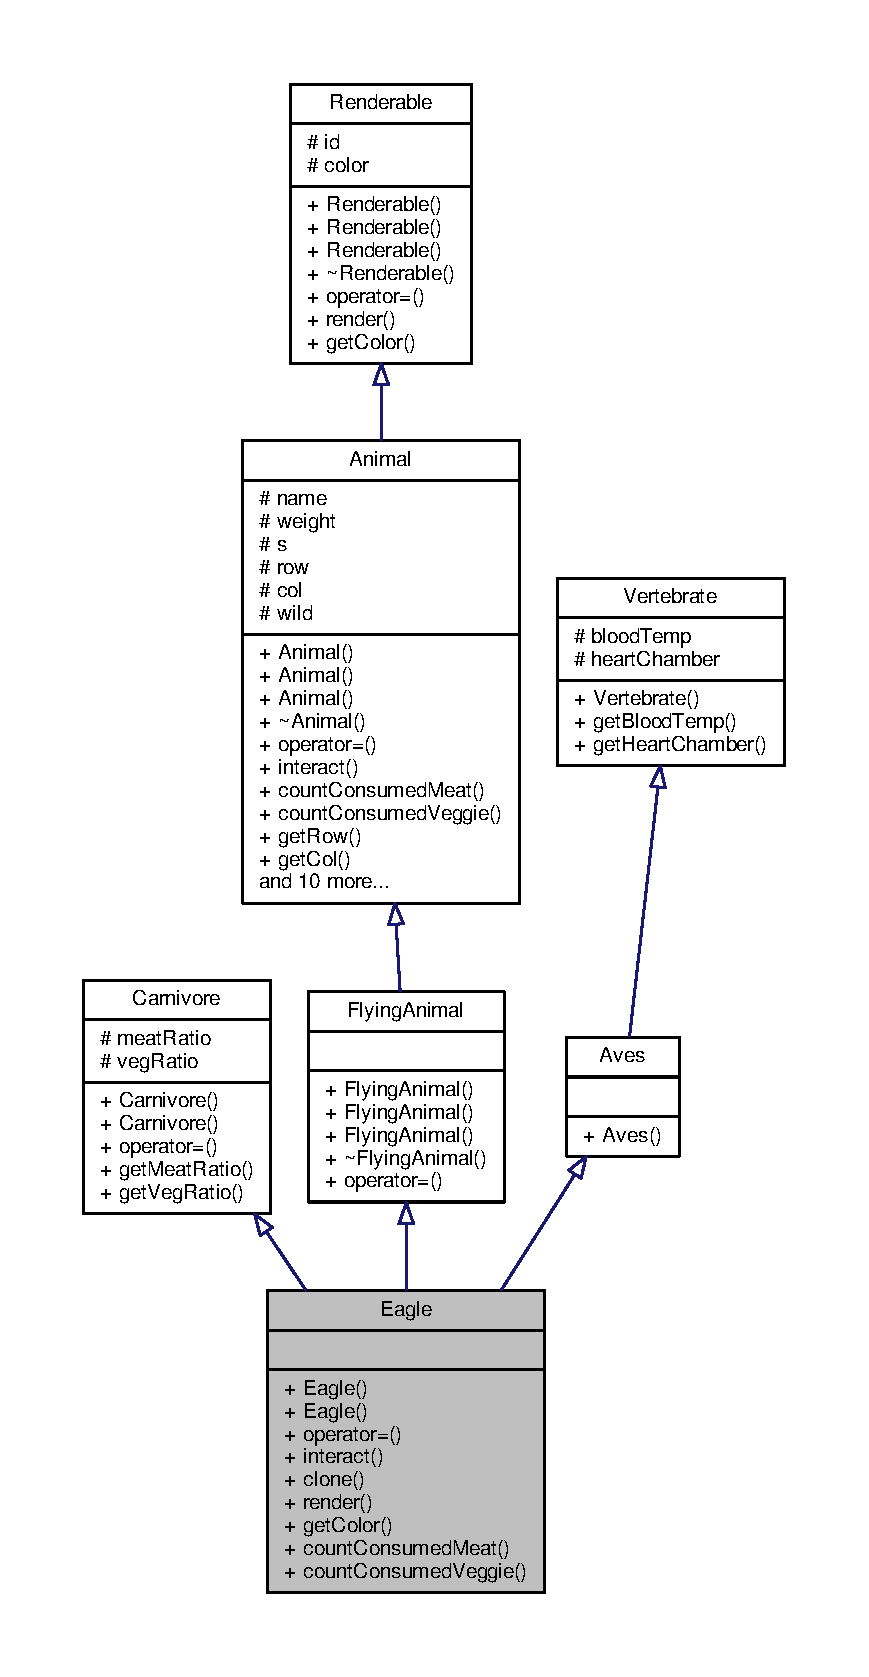
\includegraphics[height=550pt]{classEagle__inherit__graph}
\end{center}
\end{figure}


Collaboration diagram for Eagle\+:
\nopagebreak
\begin{figure}[H]
\begin{center}
\leavevmode
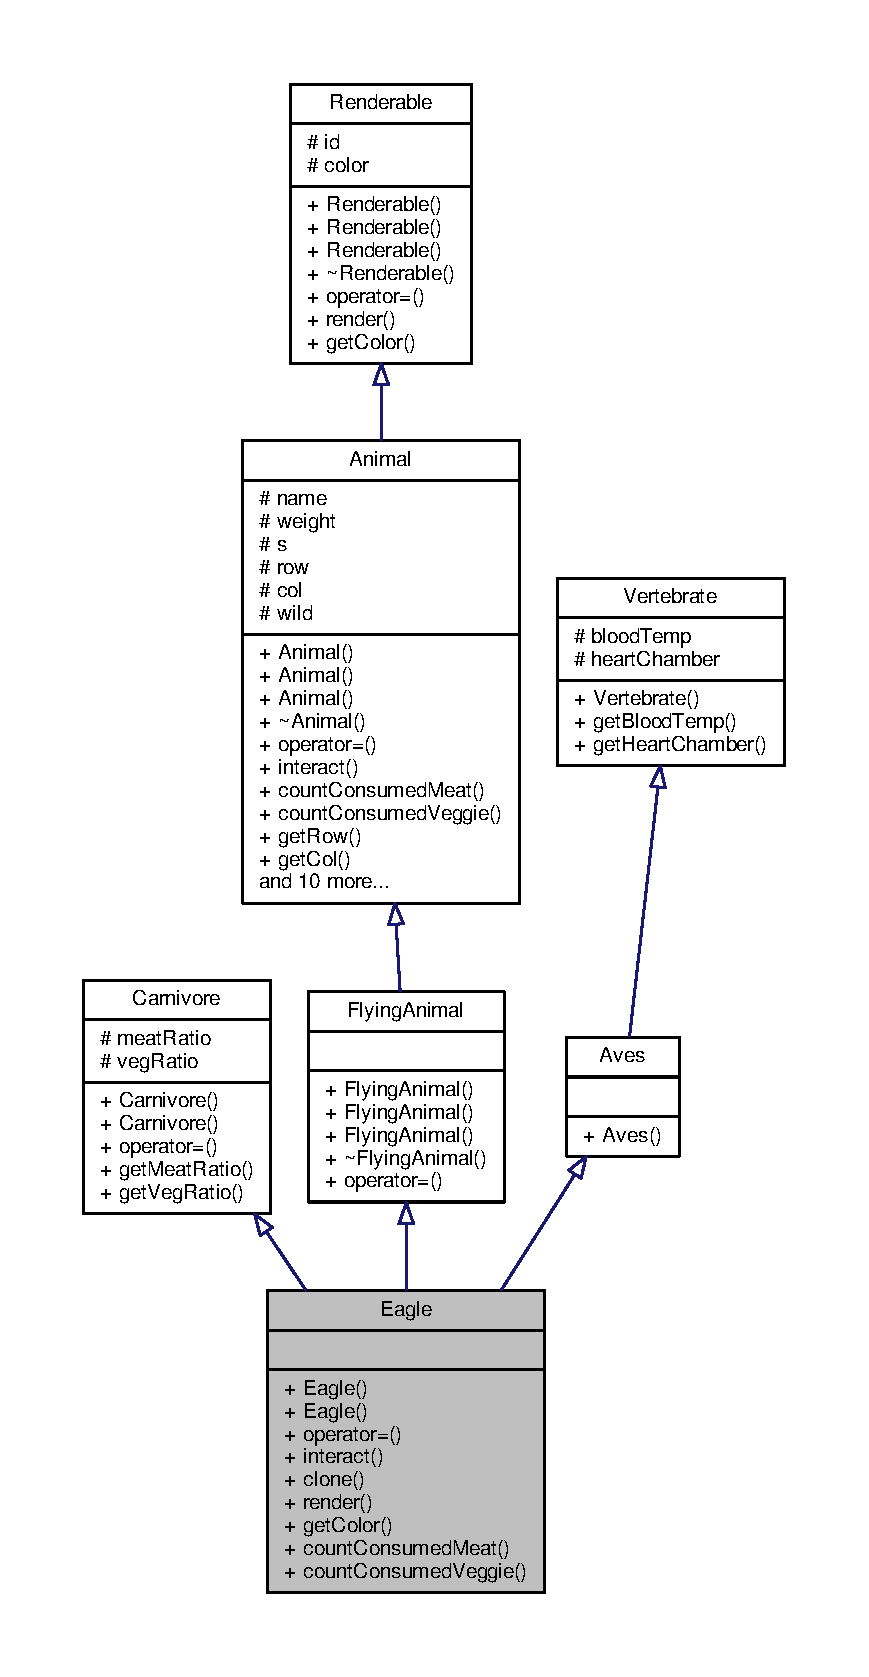
\includegraphics[height=550pt]{classEagle__coll__graph}
\end{center}
\end{figure}
\subsection*{Public Member Functions}
\begin{DoxyCompactItemize}
\item 
\hyperlink{classEagle_aae9a6a5e49f7eb52e598ad9671973cd1}{Eagle} (string \+\_\+name, double \+\_\+weight, \hyperlink{sex_8h_a2633cb393c68bb2ee8080db58fb7ba93}{Sex} \+\_\+s, int \+\_\+r, int \+\_\+c)
\begin{DoxyCompactList}\small\item\em Consructor. \end{DoxyCompactList}\item 
\hyperlink{classEagle_a7255de3683837e66642f9969b06a2c0c}{Eagle} (const \hyperlink{classEagle}{Eagle} \&E)
\begin{DoxyCompactList}\small\item\em Copy Consructor. \end{DoxyCompactList}\item 
\hyperlink{classEagle}{Eagle} \& \hyperlink{classEagle_a26fa818d2c6168304fe6eb7fd80b5ab7}{operator=} (const \hyperlink{classEagle}{Eagle} \&E)
\begin{DoxyCompactList}\small\item\em Operator=. Melakukan assignment pada objek. \end{DoxyCompactList}\item 
virtual void \hyperlink{classEagle_aa47ed62d92f1b2f9bad339b8521a50f6}{interact} ()
\begin{DoxyCompactList}\small\item\em interact. Menampilkan interaksi hewan ke layar \end{DoxyCompactList}\item 
virtual \hyperlink{classEagle}{Eagle} $\ast$ \hyperlink{classEagle_a8b6f062eccca508c551b27c1581e7d83}{clone} () const 
\begin{DoxyCompactList}\small\item\em clone Menduplikat diri sendiri \end{DoxyCompactList}\item 
virtual char \hyperlink{classEagle_a1a97b6a2a2dbe76a6ddf3dc15e5f36d4}{render} ()
\begin{DoxyCompactList}\small\item\em render Mengembalikan karakter id tiap hewan \end{DoxyCompactList}\item 
virtual \hyperlink{color_8h_ab87bacfdad76e61b9412d7124be44c1c}{Color} \hyperlink{classEagle_ac70f5c248aca36e5c3b7f64160bc139d}{get\+Color} ()
\begin{DoxyCompactList}\small\item\em get\+Color Mengembalikan warna dari hewan \end{DoxyCompactList}\item 
virtual double \hyperlink{classEagle_a815be21cd5e4e1716a36c39eda33b686}{count\+Consumed\+Meat} ()
\begin{DoxyCompactList}\small\item\em count\+Consumed\+Meat Mengembalikan jumlah daging yang dikonsumsi \end{DoxyCompactList}\item 
virtual double \hyperlink{classEagle_a5f27f80f81ed438bf9de8a84c24765fb}{count\+Consumed\+Veggie} ()
\begin{DoxyCompactList}\small\item\em count\+Consumed\+Veggie Mengembalikan jumlah makanan tumbuhan yang dikonsumsi \end{DoxyCompactList}\end{DoxyCompactItemize}
\subsection*{Additional Inherited Members}


\subsection{Constructor \& Destructor Documentation}
\index{Eagle@{Eagle}!Eagle@{Eagle}}
\index{Eagle@{Eagle}!Eagle@{Eagle}}
\subsubsection[{\texorpdfstring{Eagle(string \+\_\+name, double \+\_\+weight, Sex \+\_\+s, int \+\_\+r, int \+\_\+c)}{Eagle(string _name, double _weight, Sex _s, int _r, int _c)}}]{\setlength{\rightskip}{0pt plus 5cm}Eagle\+::\+Eagle (
\begin{DoxyParamCaption}
\item[{string}]{\+\_\+name, }
\item[{double}]{\+\_\+weight, }
\item[{{\bf Sex}}]{\+\_\+s, }
\item[{int}]{\+\_\+r, }
\item[{int}]{\+\_\+c}
\end{DoxyParamCaption}
)}\hypertarget{classEagle_aae9a6a5e49f7eb52e598ad9671973cd1}{}\label{classEagle_aae9a6a5e49f7eb52e598ad9671973cd1}


Consructor. 


\begin{DoxyParams}{Parameters}
{\em \+\_\+name} & nama binatang \\
\hline
{\em \+\_\+weight} & berat \\
\hline
{\em \+\_\+s} & jenis kelamin \\
\hline
\end{DoxyParams}
\index{Eagle@{Eagle}!Eagle@{Eagle}}
\index{Eagle@{Eagle}!Eagle@{Eagle}}
\subsubsection[{\texorpdfstring{Eagle(const Eagle \&\+E)}{Eagle(const Eagle &E)}}]{\setlength{\rightskip}{0pt plus 5cm}Eagle\+::\+Eagle (
\begin{DoxyParamCaption}
\item[{const {\bf Eagle} \&}]{E}
\end{DoxyParamCaption}
)}\hypertarget{classEagle_a7255de3683837e66642f9969b06a2c0c}{}\label{classEagle_a7255de3683837e66642f9969b06a2c0c}


Copy Consructor. 


\begin{DoxyParams}{Parameters}
{\em E} & objek yang akan disalin \\
\hline
\end{DoxyParams}


\subsection{Member Function Documentation}
\index{Eagle@{Eagle}!clone@{clone}}
\index{clone@{clone}!Eagle@{Eagle}}
\subsubsection[{\texorpdfstring{clone() const }{clone() const }}]{\setlength{\rightskip}{0pt plus 5cm}{\bf Eagle} $\ast$ Eagle\+::clone (
\begin{DoxyParamCaption}
{}
\end{DoxyParamCaption}
) const\hspace{0.3cm}{\ttfamily [virtual]}}\hypertarget{classEagle_a8b6f062eccca508c551b27c1581e7d83}{}\label{classEagle_a8b6f062eccca508c551b27c1581e7d83}


clone Menduplikat diri sendiri 

\begin{DoxyReturn}{Returns}
value object hasil kloning 
\end{DoxyReturn}


Implements \hyperlink{classAnimal_a1430e040ea4ff43bc453fa0ad19c308d}{Animal}.

\index{Eagle@{Eagle}!count\+Consumed\+Meat@{count\+Consumed\+Meat}}
\index{count\+Consumed\+Meat@{count\+Consumed\+Meat}!Eagle@{Eagle}}
\subsubsection[{\texorpdfstring{count\+Consumed\+Meat()}{countConsumedMeat()}}]{\setlength{\rightskip}{0pt plus 5cm}double Eagle\+::count\+Consumed\+Meat (
\begin{DoxyParamCaption}
{}
\end{DoxyParamCaption}
)\hspace{0.3cm}{\ttfamily [virtual]}}\hypertarget{classEagle_a815be21cd5e4e1716a36c39eda33b686}{}\label{classEagle_a815be21cd5e4e1716a36c39eda33b686}


count\+Consumed\+Meat Mengembalikan jumlah daging yang dikonsumsi 

\begin{DoxyReturn}{Returns}
jumlah daging yang dikonsumsi 
\end{DoxyReturn}


Implements \hyperlink{classAnimal_a84ccc380d237650f2bf24d792627d376}{Animal}.

\index{Eagle@{Eagle}!count\+Consumed\+Veggie@{count\+Consumed\+Veggie}}
\index{count\+Consumed\+Veggie@{count\+Consumed\+Veggie}!Eagle@{Eagle}}
\subsubsection[{\texorpdfstring{count\+Consumed\+Veggie()}{countConsumedVeggie()}}]{\setlength{\rightskip}{0pt plus 5cm}double Eagle\+::count\+Consumed\+Veggie (
\begin{DoxyParamCaption}
{}
\end{DoxyParamCaption}
)\hspace{0.3cm}{\ttfamily [virtual]}}\hypertarget{classEagle_a5f27f80f81ed438bf9de8a84c24765fb}{}\label{classEagle_a5f27f80f81ed438bf9de8a84c24765fb}


count\+Consumed\+Veggie Mengembalikan jumlah makanan tumbuhan yang dikonsumsi 

\begin{DoxyReturn}{Returns}
jumlah makanan tumbuhan yang dikonsumsi 
\end{DoxyReturn}


Implements \hyperlink{classAnimal_aaa7e4bdb7f5a10060b6dcaf09215f822}{Animal}.

\index{Eagle@{Eagle}!get\+Color@{get\+Color}}
\index{get\+Color@{get\+Color}!Eagle@{Eagle}}
\subsubsection[{\texorpdfstring{get\+Color()}{getColor()}}]{\setlength{\rightskip}{0pt plus 5cm}{\bf Color} Eagle\+::get\+Color (
\begin{DoxyParamCaption}
{}
\end{DoxyParamCaption}
)\hspace{0.3cm}{\ttfamily [virtual]}}\hypertarget{classEagle_ac70f5c248aca36e5c3b7f64160bc139d}{}\label{classEagle_ac70f5c248aca36e5c3b7f64160bc139d}


get\+Color Mengembalikan warna dari hewan 

\begin{DoxyReturn}{Returns}
warna cetak hewan 
\end{DoxyReturn}


Implements \hyperlink{classRenderable_ab3bcc93b20929c6e92b64223344a73d5}{Renderable}.

\index{Eagle@{Eagle}!interact@{interact}}
\index{interact@{interact}!Eagle@{Eagle}}
\subsubsection[{\texorpdfstring{interact()}{interact()}}]{\setlength{\rightskip}{0pt plus 5cm}void Eagle\+::interact (
\begin{DoxyParamCaption}
{}
\end{DoxyParamCaption}
)\hspace{0.3cm}{\ttfamily [virtual]}}\hypertarget{classEagle_aa47ed62d92f1b2f9bad339b8521a50f6}{}\label{classEagle_aa47ed62d92f1b2f9bad339b8521a50f6}


interact. Menampilkan interaksi hewan ke layar 



Implements \hyperlink{classAnimal_af47626b050b665e9a19525227d2b840f}{Animal}.

\index{Eagle@{Eagle}!operator=@{operator=}}
\index{operator=@{operator=}!Eagle@{Eagle}}
\subsubsection[{\texorpdfstring{operator=(const Eagle \&\+E)}{operator=(const Eagle &E)}}]{\setlength{\rightskip}{0pt plus 5cm}{\bf Eagle} \& Eagle\+::operator= (
\begin{DoxyParamCaption}
\item[{const {\bf Eagle} \&}]{E}
\end{DoxyParamCaption}
)}\hypertarget{classEagle_a26fa818d2c6168304fe6eb7fd80b5ab7}{}\label{classEagle_a26fa818d2c6168304fe6eb7fd80b5ab7}


Operator=. Melakukan assignment pada objek. 


\begin{DoxyParams}{Parameters}
{\em E} & objek yang akan disalin \\
\hline
\end{DoxyParams}
\index{Eagle@{Eagle}!render@{render}}
\index{render@{render}!Eagle@{Eagle}}
\subsubsection[{\texorpdfstring{render()}{render()}}]{\setlength{\rightskip}{0pt plus 5cm}char Eagle\+::render (
\begin{DoxyParamCaption}
{}
\end{DoxyParamCaption}
)\hspace{0.3cm}{\ttfamily [virtual]}}\hypertarget{classEagle_a1a97b6a2a2dbe76a6ddf3dc15e5f36d4}{}\label{classEagle_a1a97b6a2a2dbe76a6ddf3dc15e5f36d4}


render Mengembalikan karakter id tiap hewan 

\begin{DoxyReturn}{Returns}
karakter tiap hewan 
\end{DoxyReturn}


Implements \hyperlink{classRenderable_aafa9280e6dcfa557b3cd675221fd97b4}{Renderable}.



The documentation for this class was generated from the following files\+:\begin{DoxyCompactItemize}
\item 
src/renders/animals/\hyperlink{species_8h}{species.\+h}\item 
src/renders/animals/\hyperlink{species_8cpp}{species.\+cpp}\end{DoxyCompactItemize}

\hypertarget{classElephant}{}\section{Elephant Class Reference}
\label{classElephant}\index{Elephant@{Elephant}}


{\ttfamily \#include $<$species.\+h$>$}



Inheritance diagram for Elephant\+:
\nopagebreak
\begin{figure}[H]
\begin{center}
\leavevmode
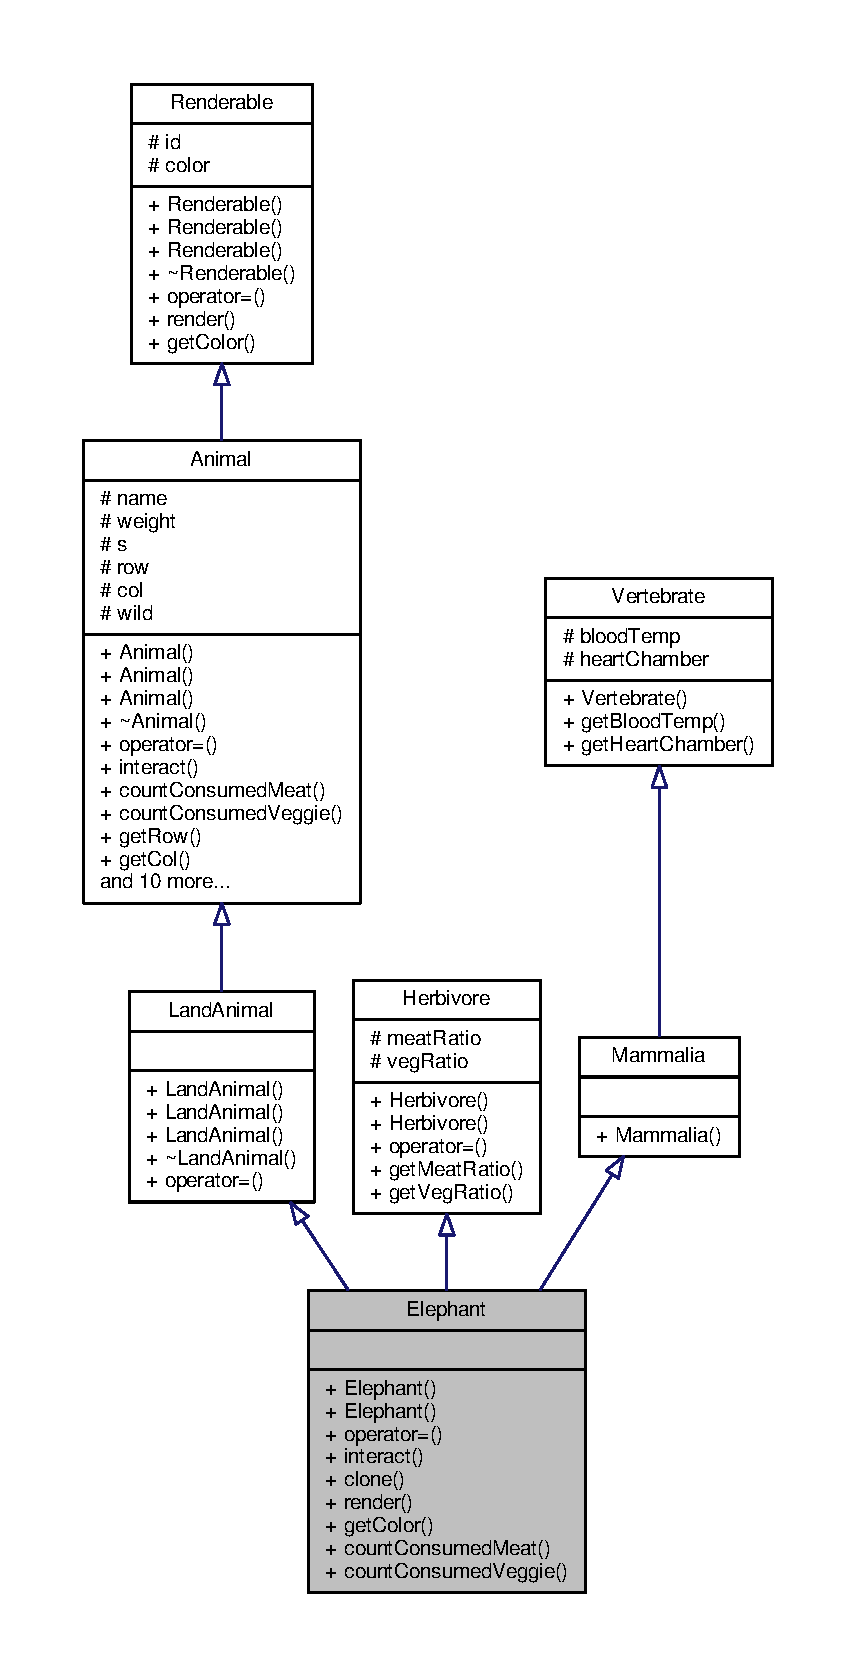
\includegraphics[height=550pt]{classElephant__inherit__graph}
\end{center}
\end{figure}


Collaboration diagram for Elephant\+:
\nopagebreak
\begin{figure}[H]
\begin{center}
\leavevmode
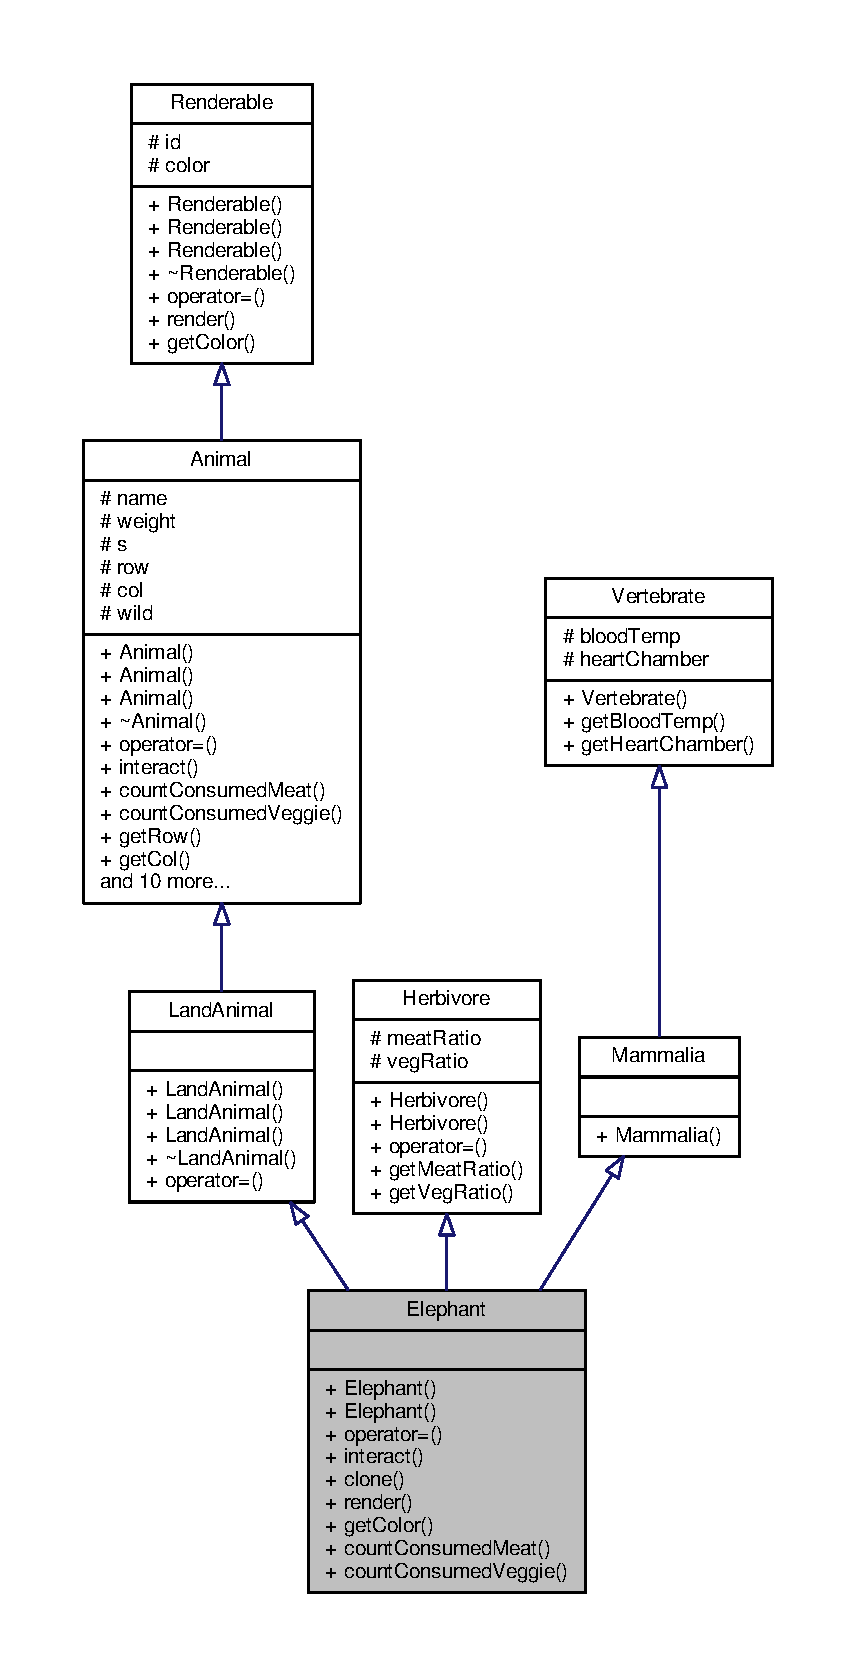
\includegraphics[height=550pt]{classElephant__coll__graph}
\end{center}
\end{figure}
\subsection*{Public Member Functions}
\begin{DoxyCompactItemize}
\item 
\hyperlink{classElephant_a7a94c60757db4cfc466fb14be048472e}{Elephant} (string \+\_\+name, double \+\_\+weight, \hyperlink{sex_8h_a2633cb393c68bb2ee8080db58fb7ba93}{Sex} \+\_\+s, int \+\_\+r, int \+\_\+c)
\begin{DoxyCompactList}\small\item\em Consructor. \end{DoxyCompactList}\item 
\hyperlink{classElephant_a1ca9260043931fcd63f2be2694e74ead}{Elephant} (const \hyperlink{classElephant}{Elephant} \&E)
\begin{DoxyCompactList}\small\item\em Copy Consructor. \end{DoxyCompactList}\item 
\hyperlink{classElephant}{Elephant} \& \hyperlink{classElephant_a822345b7b81981324451feb7603fdf07}{operator=} (const \hyperlink{classElephant}{Elephant} \&E)
\begin{DoxyCompactList}\small\item\em Operator=. Melakukan assignment pada objek. \end{DoxyCompactList}\item 
virtual void \hyperlink{classElephant_a26c7fe6f59e30b8cf400004edd2d3196}{interact} ()
\begin{DoxyCompactList}\small\item\em interact. Menampilkan interaksi hewan ke layar \end{DoxyCompactList}\item 
virtual \hyperlink{classElephant}{Elephant} $\ast$ \hyperlink{classElephant_a5f3470439cfb819eb68a8ebc070ffaee}{clone} () const 
\begin{DoxyCompactList}\small\item\em clone Menduplikat diri sendiri \end{DoxyCompactList}\item 
virtual char \hyperlink{classElephant_a96ae3a5917af96a358079c57e0b2e3b5}{render} ()
\begin{DoxyCompactList}\small\item\em render Mengembalikan karakter id tiap hewan \end{DoxyCompactList}\item 
virtual \hyperlink{color_8h_ab87bacfdad76e61b9412d7124be44c1c}{Color} \hyperlink{classElephant_a85d7fa33bebc6fc766b8d229a9f6f50f}{get\+Color} ()
\begin{DoxyCompactList}\small\item\em get\+Color Mengembalikan warna dari hewan \end{DoxyCompactList}\item 
virtual double \hyperlink{classElephant_ab210c0612d4e9ab539dc47a0776a8997}{count\+Consumed\+Meat} ()
\begin{DoxyCompactList}\small\item\em count\+Consumed\+Meat Mengembalikan jumlah daging yang dikonsumsi \end{DoxyCompactList}\item 
virtual double \hyperlink{classElephant_a2919bc91970a375001341d63526590c5}{count\+Consumed\+Veggie} ()
\begin{DoxyCompactList}\small\item\em count\+Consumed\+Veggie Mengembalikan jumlah makanan tumbuhan yang dikonsumsi \end{DoxyCompactList}\end{DoxyCompactItemize}
\subsection*{Additional Inherited Members}


\subsection{Constructor \& Destructor Documentation}
\index{Elephant@{Elephant}!Elephant@{Elephant}}
\index{Elephant@{Elephant}!Elephant@{Elephant}}
\subsubsection[{\texorpdfstring{Elephant(string \+\_\+name, double \+\_\+weight, Sex \+\_\+s, int \+\_\+r, int \+\_\+c)}{Elephant(string _name, double _weight, Sex _s, int _r, int _c)}}]{\setlength{\rightskip}{0pt plus 5cm}Elephant\+::\+Elephant (
\begin{DoxyParamCaption}
\item[{string}]{\+\_\+name, }
\item[{double}]{\+\_\+weight, }
\item[{{\bf Sex}}]{\+\_\+s, }
\item[{int}]{\+\_\+r, }
\item[{int}]{\+\_\+c}
\end{DoxyParamCaption}
)}\hypertarget{classElephant_a7a94c60757db4cfc466fb14be048472e}{}\label{classElephant_a7a94c60757db4cfc466fb14be048472e}


Consructor. 


\begin{DoxyParams}{Parameters}
{\em \+\_\+name} & nama binatang \\
\hline
{\em \+\_\+weight} & berat \\
\hline
{\em \+\_\+s} & jenis kelamin \\
\hline
\end{DoxyParams}
\index{Elephant@{Elephant}!Elephant@{Elephant}}
\index{Elephant@{Elephant}!Elephant@{Elephant}}
\subsubsection[{\texorpdfstring{Elephant(const Elephant \&\+E)}{Elephant(const Elephant &E)}}]{\setlength{\rightskip}{0pt plus 5cm}Elephant\+::\+Elephant (
\begin{DoxyParamCaption}
\item[{const {\bf Elephant} \&}]{E}
\end{DoxyParamCaption}
)}\hypertarget{classElephant_a1ca9260043931fcd63f2be2694e74ead}{}\label{classElephant_a1ca9260043931fcd63f2be2694e74ead}


Copy Consructor. 


\begin{DoxyParams}{Parameters}
{\em E} & objek yang akan disalin \\
\hline
\end{DoxyParams}


\subsection{Member Function Documentation}
\index{Elephant@{Elephant}!clone@{clone}}
\index{clone@{clone}!Elephant@{Elephant}}
\subsubsection[{\texorpdfstring{clone() const }{clone() const }}]{\setlength{\rightskip}{0pt plus 5cm}{\bf Elephant} $\ast$ Elephant\+::clone (
\begin{DoxyParamCaption}
{}
\end{DoxyParamCaption}
) const\hspace{0.3cm}{\ttfamily [virtual]}}\hypertarget{classElephant_a5f3470439cfb819eb68a8ebc070ffaee}{}\label{classElephant_a5f3470439cfb819eb68a8ebc070ffaee}


clone Menduplikat diri sendiri 

\begin{DoxyReturn}{Returns}
value object hasil kloning 
\end{DoxyReturn}


Implements \hyperlink{classAnimal_a1430e040ea4ff43bc453fa0ad19c308d}{Animal}.

\index{Elephant@{Elephant}!count\+Consumed\+Meat@{count\+Consumed\+Meat}}
\index{count\+Consumed\+Meat@{count\+Consumed\+Meat}!Elephant@{Elephant}}
\subsubsection[{\texorpdfstring{count\+Consumed\+Meat()}{countConsumedMeat()}}]{\setlength{\rightskip}{0pt plus 5cm}double Elephant\+::count\+Consumed\+Meat (
\begin{DoxyParamCaption}
{}
\end{DoxyParamCaption}
)\hspace{0.3cm}{\ttfamily [virtual]}}\hypertarget{classElephant_ab210c0612d4e9ab539dc47a0776a8997}{}\label{classElephant_ab210c0612d4e9ab539dc47a0776a8997}


count\+Consumed\+Meat Mengembalikan jumlah daging yang dikonsumsi 

\begin{DoxyReturn}{Returns}
jumlah daging yang dikonsumsi 
\end{DoxyReturn}


Implements \hyperlink{classAnimal_a84ccc380d237650f2bf24d792627d376}{Animal}.

\index{Elephant@{Elephant}!count\+Consumed\+Veggie@{count\+Consumed\+Veggie}}
\index{count\+Consumed\+Veggie@{count\+Consumed\+Veggie}!Elephant@{Elephant}}
\subsubsection[{\texorpdfstring{count\+Consumed\+Veggie()}{countConsumedVeggie()}}]{\setlength{\rightskip}{0pt plus 5cm}double Elephant\+::count\+Consumed\+Veggie (
\begin{DoxyParamCaption}
{}
\end{DoxyParamCaption}
)\hspace{0.3cm}{\ttfamily [virtual]}}\hypertarget{classElephant_a2919bc91970a375001341d63526590c5}{}\label{classElephant_a2919bc91970a375001341d63526590c5}


count\+Consumed\+Veggie Mengembalikan jumlah makanan tumbuhan yang dikonsumsi 

\begin{DoxyReturn}{Returns}
jumlah makanan tumbuhan yang dikonsumsi 
\end{DoxyReturn}


Implements \hyperlink{classAnimal_aaa7e4bdb7f5a10060b6dcaf09215f822}{Animal}.

\index{Elephant@{Elephant}!get\+Color@{get\+Color}}
\index{get\+Color@{get\+Color}!Elephant@{Elephant}}
\subsubsection[{\texorpdfstring{get\+Color()}{getColor()}}]{\setlength{\rightskip}{0pt plus 5cm}{\bf Color} Elephant\+::get\+Color (
\begin{DoxyParamCaption}
{}
\end{DoxyParamCaption}
)\hspace{0.3cm}{\ttfamily [virtual]}}\hypertarget{classElephant_a85d7fa33bebc6fc766b8d229a9f6f50f}{}\label{classElephant_a85d7fa33bebc6fc766b8d229a9f6f50f}


get\+Color Mengembalikan warna dari hewan 

\begin{DoxyReturn}{Returns}
warna cetak hewan 
\end{DoxyReturn}


Implements \hyperlink{classRenderable_ab3bcc93b20929c6e92b64223344a73d5}{Renderable}.

\index{Elephant@{Elephant}!interact@{interact}}
\index{interact@{interact}!Elephant@{Elephant}}
\subsubsection[{\texorpdfstring{interact()}{interact()}}]{\setlength{\rightskip}{0pt plus 5cm}void Elephant\+::interact (
\begin{DoxyParamCaption}
{}
\end{DoxyParamCaption}
)\hspace{0.3cm}{\ttfamily [virtual]}}\hypertarget{classElephant_a26c7fe6f59e30b8cf400004edd2d3196}{}\label{classElephant_a26c7fe6f59e30b8cf400004edd2d3196}


interact. Menampilkan interaksi hewan ke layar 



Implements \hyperlink{classAnimal_af47626b050b665e9a19525227d2b840f}{Animal}.

\index{Elephant@{Elephant}!operator=@{operator=}}
\index{operator=@{operator=}!Elephant@{Elephant}}
\subsubsection[{\texorpdfstring{operator=(const Elephant \&\+E)}{operator=(const Elephant &E)}}]{\setlength{\rightskip}{0pt plus 5cm}{\bf Elephant} \& Elephant\+::operator= (
\begin{DoxyParamCaption}
\item[{const {\bf Elephant} \&}]{E}
\end{DoxyParamCaption}
)}\hypertarget{classElephant_a822345b7b81981324451feb7603fdf07}{}\label{classElephant_a822345b7b81981324451feb7603fdf07}


Operator=. Melakukan assignment pada objek. 


\begin{DoxyParams}{Parameters}
{\em E} & objek yang akan disalin \\
\hline
\end{DoxyParams}
\index{Elephant@{Elephant}!render@{render}}
\index{render@{render}!Elephant@{Elephant}}
\subsubsection[{\texorpdfstring{render()}{render()}}]{\setlength{\rightskip}{0pt plus 5cm}char Elephant\+::render (
\begin{DoxyParamCaption}
{}
\end{DoxyParamCaption}
)\hspace{0.3cm}{\ttfamily [virtual]}}\hypertarget{classElephant_a96ae3a5917af96a358079c57e0b2e3b5}{}\label{classElephant_a96ae3a5917af96a358079c57e0b2e3b5}


render Mengembalikan karakter id tiap hewan 

\begin{DoxyReturn}{Returns}
karakter tiap hewan 
\end{DoxyReturn}


Implements \hyperlink{classRenderable_aafa9280e6dcfa557b3cd675221fd97b4}{Renderable}.



The documentation for this class was generated from the following files\+:\begin{DoxyCompactItemize}
\item 
src/renders/animals/\hyperlink{species_8h}{species.\+h}\item 
src/renders/animals/\hyperlink{species_8cpp}{species.\+cpp}\end{DoxyCompactItemize}

\hypertarget{classEntrance}{}\section{Entrance Class Reference}
\label{classEntrance}\index{Entrance@{Entrance}}


{\ttfamily \#include $<$entrance.\+h$>$}



Inheritance diagram for Entrance\+:
\nopagebreak
\begin{figure}[H]
\begin{center}
\leavevmode
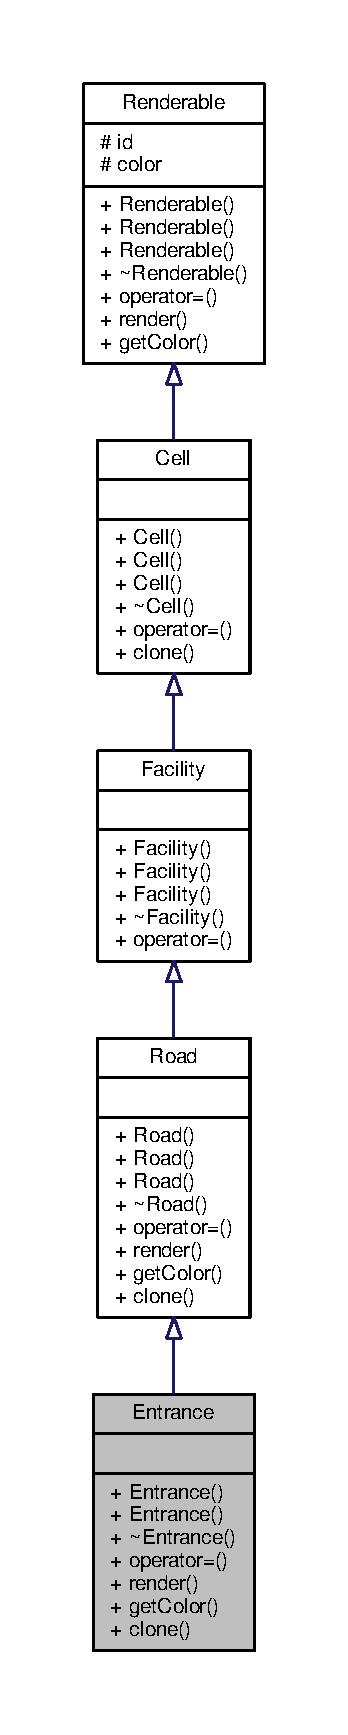
\includegraphics[height=550pt]{classEntrance__inherit__graph}
\end{center}
\end{figure}


Collaboration diagram for Entrance\+:
\nopagebreak
\begin{figure}[H]
\begin{center}
\leavevmode
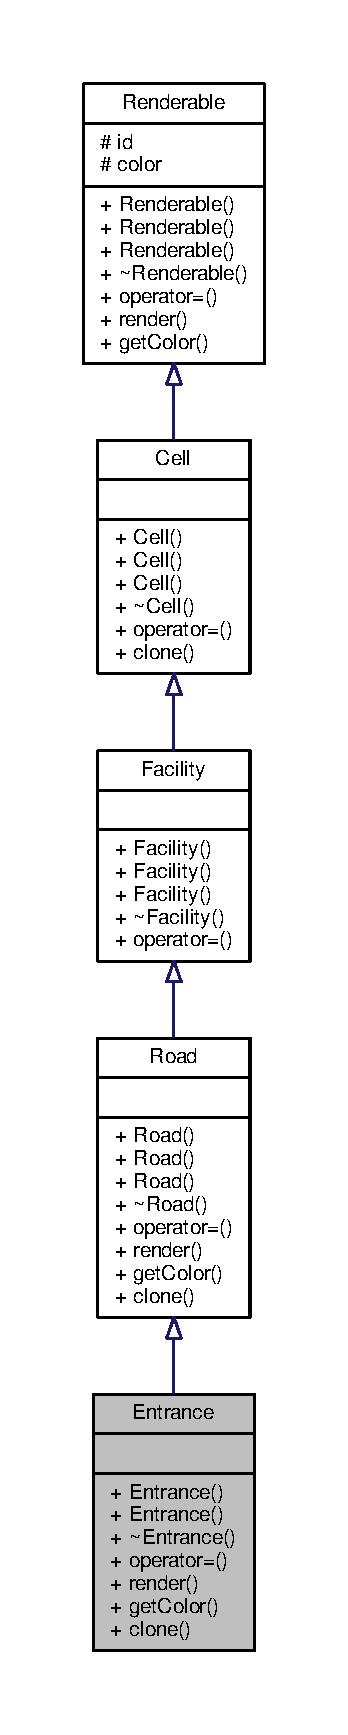
\includegraphics[height=550pt]{classEntrance__coll__graph}
\end{center}
\end{figure}
\subsection*{Public Member Functions}
\begin{DoxyCompactItemize}
\item 
\hyperlink{classEntrance_a88cd27875093371afa47ac0f321716d7}{Entrance} ()
\begin{DoxyCompactList}\small\item\em Constructor. Menciptakan \hyperlink{classEntrance}{Entrance}. \end{DoxyCompactList}\item 
\hyperlink{classEntrance_abecc3f2ef74f5e1a7304ff6778c58ab9}{Entrance} (const \hyperlink{classEntrance}{Entrance} \&)
\begin{DoxyCompactList}\small\item\em Copy Constructor. Menciptakan salinan dari \hyperlink{classEntrance}{Entrance}. \end{DoxyCompactList}\item 
virtual \hyperlink{classEntrance_a05919fe3f4948ea3266b5dd4c5e119ac}{$\sim$\+Entrance} ()
\begin{DoxyCompactList}\small\item\em Destructor. \end{DoxyCompactList}\item 
\hyperlink{classEntrance}{Entrance} \& \hyperlink{classEntrance_ac2a663bd035fd2f6c894165c4ee16a97}{operator=} (const \hyperlink{classEntrance}{Entrance} \&)
\begin{DoxyCompactList}\small\item\em Operator=. Menginisialisasi \hyperlink{classEntrance}{Entrance} tanpa terjadi bitwise copy. \end{DoxyCompactList}\item 
char \hyperlink{classEntrance_a7a2870f72aa2e300896b3fa78c8dcba9}{render} ()
\begin{DoxyCompactList}\small\item\em Render. Mengembalikan karakter untuk ditampilkan ke layar. \end{DoxyCompactList}\item 
\hyperlink{color_8h_ab87bacfdad76e61b9412d7124be44c1c}{Color} \hyperlink{classEntrance_aa0a541a0507a74635e08ccab7b9d6953}{get\+Color} ()
\begin{DoxyCompactList}\small\item\em Get\+Color. Mengembalikan warna untuk ditampilkan ke layar. \end{DoxyCompactList}\item 
virtual \hyperlink{classEntrance}{Entrance} $\ast$ \hyperlink{classEntrance_a5f20360c5b495b5ed4163deb33ff06de}{clone} () const 
\begin{DoxyCompactList}\small\item\em Clone. Menduplikat diri sendiri. \end{DoxyCompactList}\end{DoxyCompactItemize}
\subsection*{Additional Inherited Members}


\subsection{Detailed Description}
Adalah kelas anak dari \hyperlink{classRoad}{Road}. Adalah representasi dari jalan masuk ke zoo. 

\subsection{Constructor \& Destructor Documentation}
\index{Entrance@{Entrance}!Entrance@{Entrance}}
\index{Entrance@{Entrance}!Entrance@{Entrance}}
\subsubsection[{\texorpdfstring{Entrance()}{Entrance()}}]{\setlength{\rightskip}{0pt plus 5cm}Entrance\+::\+Entrance (
\begin{DoxyParamCaption}
{}
\end{DoxyParamCaption}
)}\hypertarget{classEntrance_a88cd27875093371afa47ac0f321716d7}{}\label{classEntrance_a88cd27875093371afa47ac0f321716d7}


Constructor. Menciptakan \hyperlink{classEntrance}{Entrance}. 

\index{Entrance@{Entrance}!Entrance@{Entrance}}
\index{Entrance@{Entrance}!Entrance@{Entrance}}
\subsubsection[{\texorpdfstring{Entrance(const Entrance \&)}{Entrance(const Entrance &)}}]{\setlength{\rightskip}{0pt plus 5cm}Entrance\+::\+Entrance (
\begin{DoxyParamCaption}
\item[{const {\bf Entrance} \&}]{E}
\end{DoxyParamCaption}
)}\hypertarget{classEntrance_abecc3f2ef74f5e1a7304ff6778c58ab9}{}\label{classEntrance_abecc3f2ef74f5e1a7304ff6778c58ab9}


Copy Constructor. Menciptakan salinan dari \hyperlink{classEntrance}{Entrance}. 


\begin{DoxyParams}{Parameters}
{\em E} & \hyperlink{classEntrance}{Entrance} yang ingin disalin. \\
\hline
\end{DoxyParams}
\index{Entrance@{Entrance}!````~Entrance@{$\sim$\+Entrance}}
\index{````~Entrance@{$\sim$\+Entrance}!Entrance@{Entrance}}
\subsubsection[{\texorpdfstring{$\sim$\+Entrance()}{~Entrance()}}]{\setlength{\rightskip}{0pt plus 5cm}Entrance\+::$\sim$\+Entrance (
\begin{DoxyParamCaption}
{}
\end{DoxyParamCaption}
)\hspace{0.3cm}{\ttfamily [virtual]}}\hypertarget{classEntrance_a05919fe3f4948ea3266b5dd4c5e119ac}{}\label{classEntrance_a05919fe3f4948ea3266b5dd4c5e119ac}


Destructor. 



\subsection{Member Function Documentation}
\index{Entrance@{Entrance}!clone@{clone}}
\index{clone@{clone}!Entrance@{Entrance}}
\subsubsection[{\texorpdfstring{clone() const }{clone() const }}]{\setlength{\rightskip}{0pt plus 5cm}{\bf Entrance} $\ast$ Entrance\+::clone (
\begin{DoxyParamCaption}
{}
\end{DoxyParamCaption}
) const\hspace{0.3cm}{\ttfamily [virtual]}}\hypertarget{classEntrance_a5f20360c5b495b5ed4163deb33ff06de}{}\label{classEntrance_a5f20360c5b495b5ed4163deb33ff06de}


Clone. Menduplikat diri sendiri. 

\begin{DoxyReturn}{Returns}
value object hasil kloning 
\end{DoxyReturn}


Reimplemented from \hyperlink{classRoad_a0dae048f0e2f56afa5e3fda6f30bf262}{Road}.

\index{Entrance@{Entrance}!get\+Color@{get\+Color}}
\index{get\+Color@{get\+Color}!Entrance@{Entrance}}
\subsubsection[{\texorpdfstring{get\+Color()}{getColor()}}]{\setlength{\rightskip}{0pt plus 5cm}{\bf Color} Entrance\+::get\+Color (
\begin{DoxyParamCaption}
{}
\end{DoxyParamCaption}
)\hspace{0.3cm}{\ttfamily [virtual]}}\hypertarget{classEntrance_aa0a541a0507a74635e08ccab7b9d6953}{}\label{classEntrance_aa0a541a0507a74635e08ccab7b9d6953}


Get\+Color. Mengembalikan warna untuk ditampilkan ke layar. 

\begin{DoxyReturn}{Returns}
color warna untuk dirender 
\end{DoxyReturn}


Implements \hyperlink{classRenderable_ab3bcc93b20929c6e92b64223344a73d5}{Renderable}.

\index{Entrance@{Entrance}!operator=@{operator=}}
\index{operator=@{operator=}!Entrance@{Entrance}}
\subsubsection[{\texorpdfstring{operator=(const Entrance \&)}{operator=(const Entrance &)}}]{\setlength{\rightskip}{0pt plus 5cm}{\bf Entrance} \& Entrance\+::operator= (
\begin{DoxyParamCaption}
\item[{const {\bf Entrance} \&}]{E}
\end{DoxyParamCaption}
)}\hypertarget{classEntrance_ac2a663bd035fd2f6c894165c4ee16a97}{}\label{classEntrance_ac2a663bd035fd2f6c894165c4ee16a97}


Operator=. Menginisialisasi \hyperlink{classEntrance}{Entrance} tanpa terjadi bitwise copy. 

\begin{DoxyReturn}{Returns}
\hyperlink{classEntrance}{Entrance} yang sudah di assign nilai dari current object 
\end{DoxyReturn}
\index{Entrance@{Entrance}!render@{render}}
\index{render@{render}!Entrance@{Entrance}}
\subsubsection[{\texorpdfstring{render()}{render()}}]{\setlength{\rightskip}{0pt plus 5cm}char Entrance\+::render (
\begin{DoxyParamCaption}
{}
\end{DoxyParamCaption}
)\hspace{0.3cm}{\ttfamily [virtual]}}\hypertarget{classEntrance_a7a2870f72aa2e300896b3fa78c8dcba9}{}\label{classEntrance_a7a2870f72aa2e300896b3fa78c8dcba9}


Render. Mengembalikan karakter untuk ditampilkan ke layar. 

\begin{DoxyReturn}{Returns}
id bertipe char 
\end{DoxyReturn}


Implements \hyperlink{classRenderable_aafa9280e6dcfa557b3cd675221fd97b4}{Renderable}.



The documentation for this class was generated from the following files\+:\begin{DoxyCompactItemize}
\item 
src/renders/facilities/road/entrance/\hyperlink{entrance_8h}{entrance.\+h}\item 
src/renders/facilities/road/entrance/\hyperlink{entrance_8cpp}{entrance.\+cpp}\end{DoxyCompactItemize}

\hypertarget{classExit}{}\section{Exit Class Reference}
\label{classExit}\index{Exit@{Exit}}


{\ttfamily \#include $<$exit.\+h$>$}



Inheritance diagram for Exit\+:
\nopagebreak
\begin{figure}[H]
\begin{center}
\leavevmode
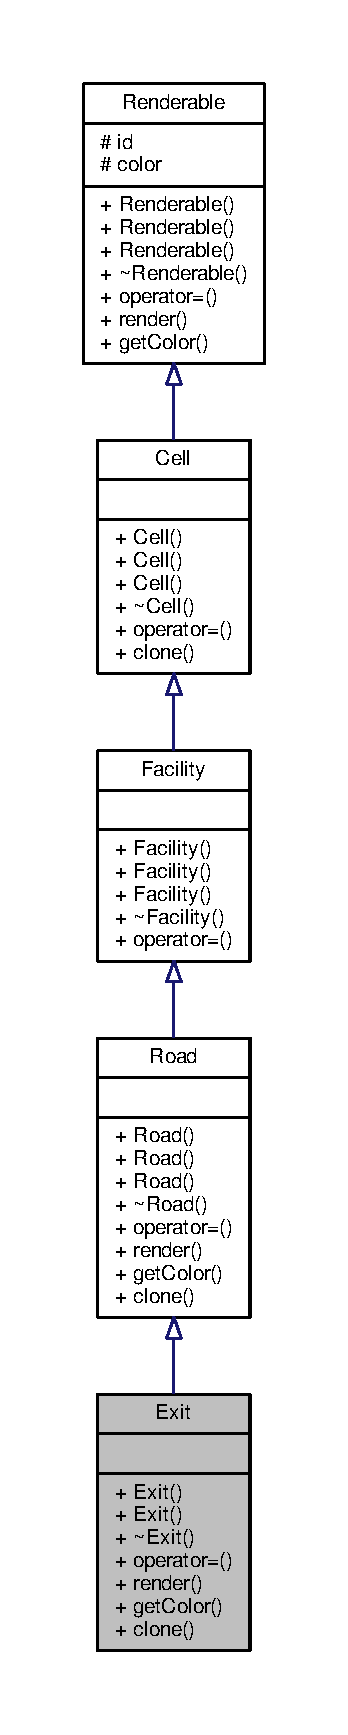
\includegraphics[height=550pt]{classExit__inherit__graph}
\end{center}
\end{figure}


Collaboration diagram for Exit\+:
\nopagebreak
\begin{figure}[H]
\begin{center}
\leavevmode
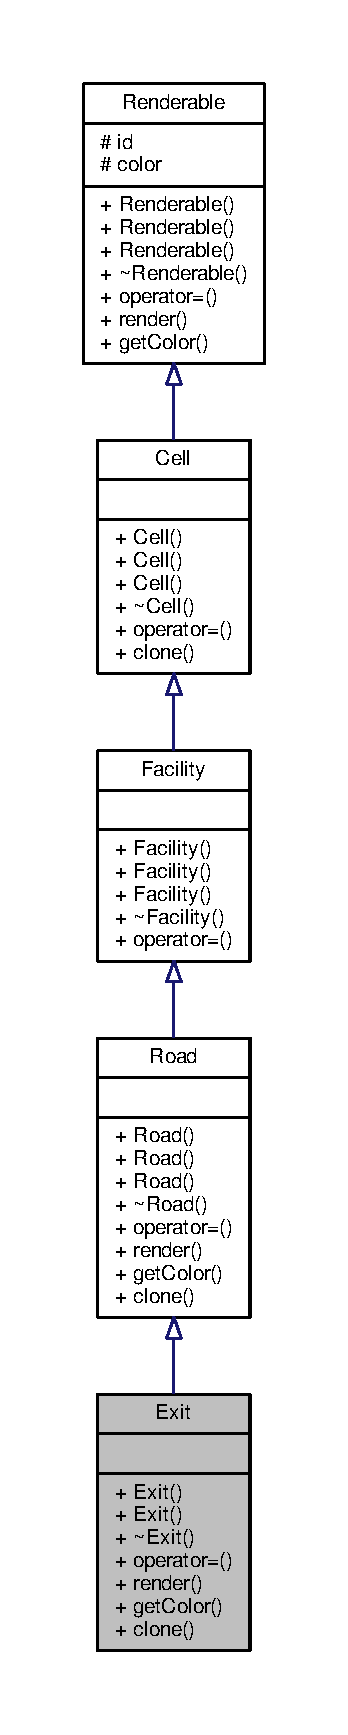
\includegraphics[height=550pt]{classExit__coll__graph}
\end{center}
\end{figure}
\subsection*{Public Member Functions}
\begin{DoxyCompactItemize}
\item 
\hyperlink{classExit_a9b2f58ee65af58d03d7004d9fc2ab264}{Exit} ()
\begin{DoxyCompactList}\small\item\em Constructor. Menciptakan \hyperlink{classExit}{Exit}. \end{DoxyCompactList}\item 
\hyperlink{classExit_a4cdd044013db87741ebc0abdabd84a16}{Exit} (const \hyperlink{classExit}{Exit} \&)
\begin{DoxyCompactList}\small\item\em Copy Constructor. Menciptakan salinan dari \hyperlink{classExit}{Exit}. \end{DoxyCompactList}\item 
virtual \hyperlink{classExit_adf66e70ca988ae2fe7e74ef256d8612a}{$\sim$\+Exit} ()
\begin{DoxyCompactList}\small\item\em Destructor. \end{DoxyCompactList}\item 
\hyperlink{classExit}{Exit} \& \hyperlink{classExit_a0267879724d7267cc38a44c97828e6eb}{operator=} (const \hyperlink{classExit}{Exit} \&)
\begin{DoxyCompactList}\small\item\em Operator=. Menginisialisasi \hyperlink{classExit}{Exit} tanpa terjadi bitwise copy. \end{DoxyCompactList}\item 
char \hyperlink{classExit_aa02d10be39e89bb4f7d7f2934829863a}{render} ()
\begin{DoxyCompactList}\small\item\em Render. Mengembalikan karakter untuk ditampilkan ke layar. \end{DoxyCompactList}\item 
\hyperlink{color_8h_ab87bacfdad76e61b9412d7124be44c1c}{Color} \hyperlink{classExit_a8a409166c560f8b72b876e3d9711769a}{get\+Color} ()
\begin{DoxyCompactList}\small\item\em Get\+Color. Mengembalikan warna untuk ditampilkan ke layar. \end{DoxyCompactList}\item 
virtual \hyperlink{classExit}{Exit} $\ast$ \hyperlink{classExit_a01a14491e2f7148b0e03b4297c60a0a0}{clone} () const 
\begin{DoxyCompactList}\small\item\em Clone. Menduplikat diri sendiri. \end{DoxyCompactList}\end{DoxyCompactItemize}
\subsection*{Additional Inherited Members}


\subsection{Detailed Description}
Adalah kelas anak dari \hyperlink{classRoad}{Road}. Adalah representasi dari jalan keluar ke zoo. 

\subsection{Constructor \& Destructor Documentation}
\index{Exit@{Exit}!Exit@{Exit}}
\index{Exit@{Exit}!Exit@{Exit}}
\subsubsection[{\texorpdfstring{Exit()}{Exit()}}]{\setlength{\rightskip}{0pt plus 5cm}Exit\+::\+Exit (
\begin{DoxyParamCaption}
{}
\end{DoxyParamCaption}
)}\hypertarget{classExit_a9b2f58ee65af58d03d7004d9fc2ab264}{}\label{classExit_a9b2f58ee65af58d03d7004d9fc2ab264}


Constructor. Menciptakan \hyperlink{classExit}{Exit}. 

\index{Exit@{Exit}!Exit@{Exit}}
\index{Exit@{Exit}!Exit@{Exit}}
\subsubsection[{\texorpdfstring{Exit(const Exit \&)}{Exit(const Exit &)}}]{\setlength{\rightskip}{0pt plus 5cm}Exit\+::\+Exit (
\begin{DoxyParamCaption}
\item[{const {\bf Exit} \&}]{E}
\end{DoxyParamCaption}
)}\hypertarget{classExit_a4cdd044013db87741ebc0abdabd84a16}{}\label{classExit_a4cdd044013db87741ebc0abdabd84a16}


Copy Constructor. Menciptakan salinan dari \hyperlink{classExit}{Exit}. 


\begin{DoxyParams}{Parameters}
{\em X} & \hyperlink{classExit}{Exit} yang ingin disalin. \\
\hline
\end{DoxyParams}
\index{Exit@{Exit}!````~Exit@{$\sim$\+Exit}}
\index{````~Exit@{$\sim$\+Exit}!Exit@{Exit}}
\subsubsection[{\texorpdfstring{$\sim$\+Exit()}{~Exit()}}]{\setlength{\rightskip}{0pt plus 5cm}Exit\+::$\sim$\+Exit (
\begin{DoxyParamCaption}
{}
\end{DoxyParamCaption}
)\hspace{0.3cm}{\ttfamily [virtual]}}\hypertarget{classExit_adf66e70ca988ae2fe7e74ef256d8612a}{}\label{classExit_adf66e70ca988ae2fe7e74ef256d8612a}


Destructor. 



\subsection{Member Function Documentation}
\index{Exit@{Exit}!clone@{clone}}
\index{clone@{clone}!Exit@{Exit}}
\subsubsection[{\texorpdfstring{clone() const }{clone() const }}]{\setlength{\rightskip}{0pt plus 5cm}{\bf Exit} $\ast$ Exit\+::clone (
\begin{DoxyParamCaption}
{}
\end{DoxyParamCaption}
) const\hspace{0.3cm}{\ttfamily [virtual]}}\hypertarget{classExit_a01a14491e2f7148b0e03b4297c60a0a0}{}\label{classExit_a01a14491e2f7148b0e03b4297c60a0a0}


Clone. Menduplikat diri sendiri. 

\begin{DoxyReturn}{Returns}
value object hasil kloning 
\end{DoxyReturn}


Reimplemented from \hyperlink{classRoad_a0dae048f0e2f56afa5e3fda6f30bf262}{Road}.

\index{Exit@{Exit}!get\+Color@{get\+Color}}
\index{get\+Color@{get\+Color}!Exit@{Exit}}
\subsubsection[{\texorpdfstring{get\+Color()}{getColor()}}]{\setlength{\rightskip}{0pt plus 5cm}{\bf Color} Exit\+::get\+Color (
\begin{DoxyParamCaption}
{}
\end{DoxyParamCaption}
)\hspace{0.3cm}{\ttfamily [virtual]}}\hypertarget{classExit_a8a409166c560f8b72b876e3d9711769a}{}\label{classExit_a8a409166c560f8b72b876e3d9711769a}


Get\+Color. Mengembalikan warna untuk ditampilkan ke layar. 

\begin{DoxyReturn}{Returns}
color warna untuk dirender 
\end{DoxyReturn}


Implements \hyperlink{classRenderable_ab3bcc93b20929c6e92b64223344a73d5}{Renderable}.

\index{Exit@{Exit}!operator=@{operator=}}
\index{operator=@{operator=}!Exit@{Exit}}
\subsubsection[{\texorpdfstring{operator=(const Exit \&)}{operator=(const Exit &)}}]{\setlength{\rightskip}{0pt plus 5cm}{\bf Exit} \& Exit\+::operator= (
\begin{DoxyParamCaption}
\item[{const {\bf Exit} \&}]{E}
\end{DoxyParamCaption}
)}\hypertarget{classExit_a0267879724d7267cc38a44c97828e6eb}{}\label{classExit_a0267879724d7267cc38a44c97828e6eb}


Operator=. Menginisialisasi \hyperlink{classExit}{Exit} tanpa terjadi bitwise copy. 

\begin{DoxyReturn}{Returns}
\hyperlink{classExit}{Exit} yang sudah di assign nilai dari current object 
\end{DoxyReturn}
\index{Exit@{Exit}!render@{render}}
\index{render@{render}!Exit@{Exit}}
\subsubsection[{\texorpdfstring{render()}{render()}}]{\setlength{\rightskip}{0pt plus 5cm}char Exit\+::render (
\begin{DoxyParamCaption}
{}
\end{DoxyParamCaption}
)\hspace{0.3cm}{\ttfamily [virtual]}}\hypertarget{classExit_aa02d10be39e89bb4f7d7f2934829863a}{}\label{classExit_aa02d10be39e89bb4f7d7f2934829863a}


Render. Mengembalikan karakter untuk ditampilkan ke layar. 

\begin{DoxyReturn}{Returns}
id bertipe char 
\end{DoxyReturn}


Implements \hyperlink{classRenderable_aafa9280e6dcfa557b3cd675221fd97b4}{Renderable}.



The documentation for this class was generated from the following files\+:\begin{DoxyCompactItemize}
\item 
src/renders/facilities/road/exit/\hyperlink{exit_8h}{exit.\+h}\item 
src/renders/facilities/road/exit/\hyperlink{exit_8cpp}{exit.\+cpp}\end{DoxyCompactItemize}

\hypertarget{classFacility}{}\section{Facility Class Reference}
\label{classFacility}\index{Facility@{Facility}}


{\ttfamily \#include $<$facility.\+h$>$}



Inheritance diagram for Facility\+:
\nopagebreak
\begin{figure}[H]
\begin{center}
\leavevmode
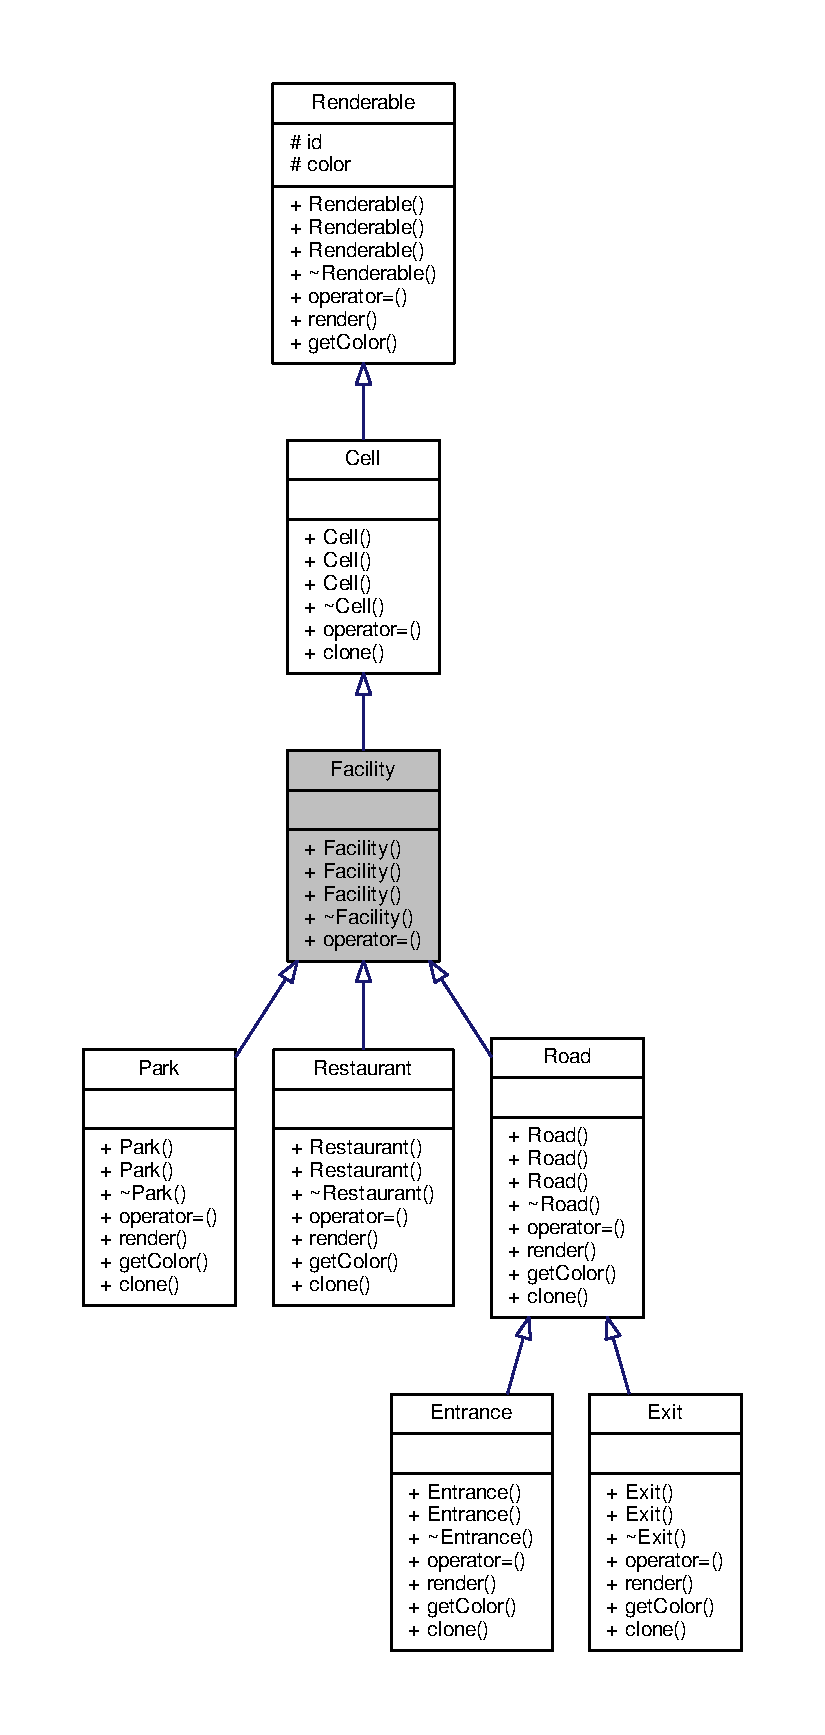
\includegraphics[height=550pt]{classFacility__inherit__graph}
\end{center}
\end{figure}


Collaboration diagram for Facility\+:
\nopagebreak
\begin{figure}[H]
\begin{center}
\leavevmode
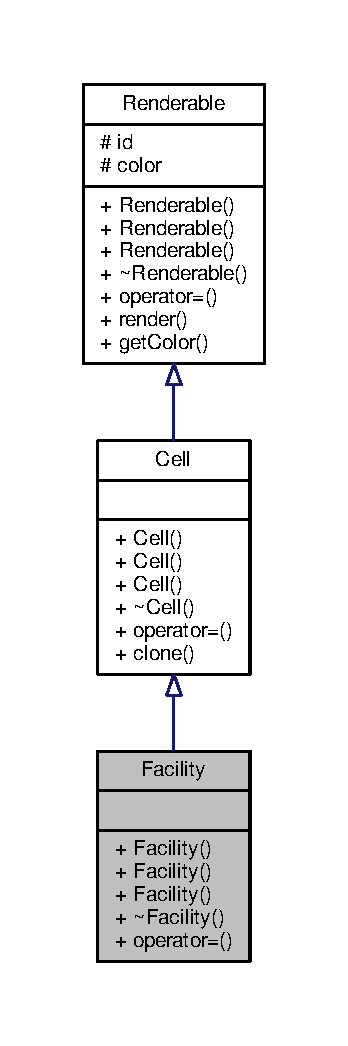
\includegraphics[width=167pt]{classFacility__coll__graph}
\end{center}
\end{figure}
\subsection*{Public Member Functions}
\begin{DoxyCompactItemize}
\item 
\hyperlink{classFacility_aea57fdf380a334f24c6861cf272b4a98}{Facility} ()
\begin{DoxyCompactList}\small\item\em Constructor. Menciptakan \hyperlink{classFacility}{Facility} kosong. \end{DoxyCompactList}\item 
\hyperlink{classFacility_a9911098ad4cc8835ec02b4c654e84c80}{Facility} (char \+\_\+id, \hyperlink{color_8h_ab87bacfdad76e61b9412d7124be44c1c}{Color} \+\_\+color)
\begin{DoxyCompactList}\small\item\em Constructor. Menciptakan \hyperlink{classFacility}{Facility} dengan parameter \+\_\+id dan \+\_\+color. \end{DoxyCompactList}\item 
\hyperlink{classFacility_aac058a14cc73b7f3fe768811a98ef045}{Facility} (const \hyperlink{classFacility}{Facility} \&)
\begin{DoxyCompactList}\small\item\em Copy Constructor. Menciptakan salinan dari \hyperlink{classFacility}{Facility}. \end{DoxyCompactList}\item 
virtual \hyperlink{classFacility_a0d756a7273f5cb2fc57575459ba45670}{$\sim$\+Facility} ()
\begin{DoxyCompactList}\small\item\em Destructor. \end{DoxyCompactList}\item 
\hyperlink{classFacility}{Facility} \& \hyperlink{classFacility_a4f7e56d32d00129e4373e6031a983530}{operator=} (const \hyperlink{classFacility}{Facility} \&)
\begin{DoxyCompactList}\small\item\em Operator=. Menginisialisasi \hyperlink{classFacility}{Facility} tanpa terjadi bitwise copy. \end{DoxyCompactList}\end{DoxyCompactItemize}
\subsection*{Additional Inherited Members}


\subsection{Detailed Description}
Adalah kelas anak dari \hyperlink{classCell}{Cell}. Adalah kelas abstrak yang merepresentasikan fasilitas zoo. 

\subsection{Constructor \& Destructor Documentation}
\index{Facility@{Facility}!Facility@{Facility}}
\index{Facility@{Facility}!Facility@{Facility}}
\subsubsection[{\texorpdfstring{Facility()}{Facility()}}]{\setlength{\rightskip}{0pt plus 5cm}Facility\+::\+Facility (
\begin{DoxyParamCaption}
{}
\end{DoxyParamCaption}
)}\hypertarget{classFacility_aea57fdf380a334f24c6861cf272b4a98}{}\label{classFacility_aea57fdf380a334f24c6861cf272b4a98}


Constructor. Menciptakan \hyperlink{classFacility}{Facility} kosong. 

\index{Facility@{Facility}!Facility@{Facility}}
\index{Facility@{Facility}!Facility@{Facility}}
\subsubsection[{\texorpdfstring{Facility(char \+\_\+id, Color \+\_\+color)}{Facility(char _id, Color _color)}}]{\setlength{\rightskip}{0pt plus 5cm}Facility\+::\+Facility (
\begin{DoxyParamCaption}
\item[{char}]{\+\_\+id, }
\item[{{\bf Color}}]{\+\_\+color}
\end{DoxyParamCaption}
)}\hypertarget{classFacility_a9911098ad4cc8835ec02b4c654e84c80}{}\label{classFacility_a9911098ad4cc8835ec02b4c654e84c80}


Constructor. Menciptakan \hyperlink{classFacility}{Facility} dengan parameter \+\_\+id dan \+\_\+color. 


\begin{DoxyParams}{Parameters}
{\em \+\_\+id} & bertipe char \\
\hline
{\em \+\_\+color} & bertipe Color \\
\hline
\end{DoxyParams}
\index{Facility@{Facility}!Facility@{Facility}}
\index{Facility@{Facility}!Facility@{Facility}}
\subsubsection[{\texorpdfstring{Facility(const Facility \&)}{Facility(const Facility &)}}]{\setlength{\rightskip}{0pt plus 5cm}Facility\+::\+Facility (
\begin{DoxyParamCaption}
\item[{const {\bf Facility} \&}]{F}
\end{DoxyParamCaption}
)}\hypertarget{classFacility_aac058a14cc73b7f3fe768811a98ef045}{}\label{classFacility_aac058a14cc73b7f3fe768811a98ef045}


Copy Constructor. Menciptakan salinan dari \hyperlink{classFacility}{Facility}. 


\begin{DoxyParams}{Parameters}
{\em F} & \hyperlink{classFacility}{Facility} yang ingin disalin. \\
\hline
\end{DoxyParams}
\index{Facility@{Facility}!````~Facility@{$\sim$\+Facility}}
\index{````~Facility@{$\sim$\+Facility}!Facility@{Facility}}
\subsubsection[{\texorpdfstring{$\sim$\+Facility()}{~Facility()}}]{\setlength{\rightskip}{0pt plus 5cm}Facility\+::$\sim$\+Facility (
\begin{DoxyParamCaption}
{}
\end{DoxyParamCaption}
)\hspace{0.3cm}{\ttfamily [virtual]}}\hypertarget{classFacility_a0d756a7273f5cb2fc57575459ba45670}{}\label{classFacility_a0d756a7273f5cb2fc57575459ba45670}


Destructor. 



\subsection{Member Function Documentation}
\index{Facility@{Facility}!operator=@{operator=}}
\index{operator=@{operator=}!Facility@{Facility}}
\subsubsection[{\texorpdfstring{operator=(const Facility \&)}{operator=(const Facility &)}}]{\setlength{\rightskip}{0pt plus 5cm}{\bf Facility} \& Facility\+::operator= (
\begin{DoxyParamCaption}
\item[{const {\bf Facility} \&}]{F}
\end{DoxyParamCaption}
)}\hypertarget{classFacility_a4f7e56d32d00129e4373e6031a983530}{}\label{classFacility_a4f7e56d32d00129e4373e6031a983530}


Operator=. Menginisialisasi \hyperlink{classFacility}{Facility} tanpa terjadi bitwise copy. 

\begin{DoxyReturn}{Returns}
\hyperlink{classFacility}{Facility} yang sudah di assign nilai dari current object 
\end{DoxyReturn}


The documentation for this class was generated from the following files\+:\begin{DoxyCompactItemize}
\item 
src/renders/facilities/\hyperlink{facility_8h}{facility.\+h}\item 
src/renders/facilities/\hyperlink{facility_8cpp}{facility.\+cpp}\end{DoxyCompactItemize}

\hypertarget{classFlyingAnimal}{}\section{Flying\+Animal Class Reference}
\label{classFlyingAnimal}\index{Flying\+Animal@{Flying\+Animal}}


{\ttfamily \#include $<$flying\+\_\+animal.\+h$>$}



Inheritance diagram for Flying\+Animal\+:
\nopagebreak
\begin{figure}[H]
\begin{center}
\leavevmode
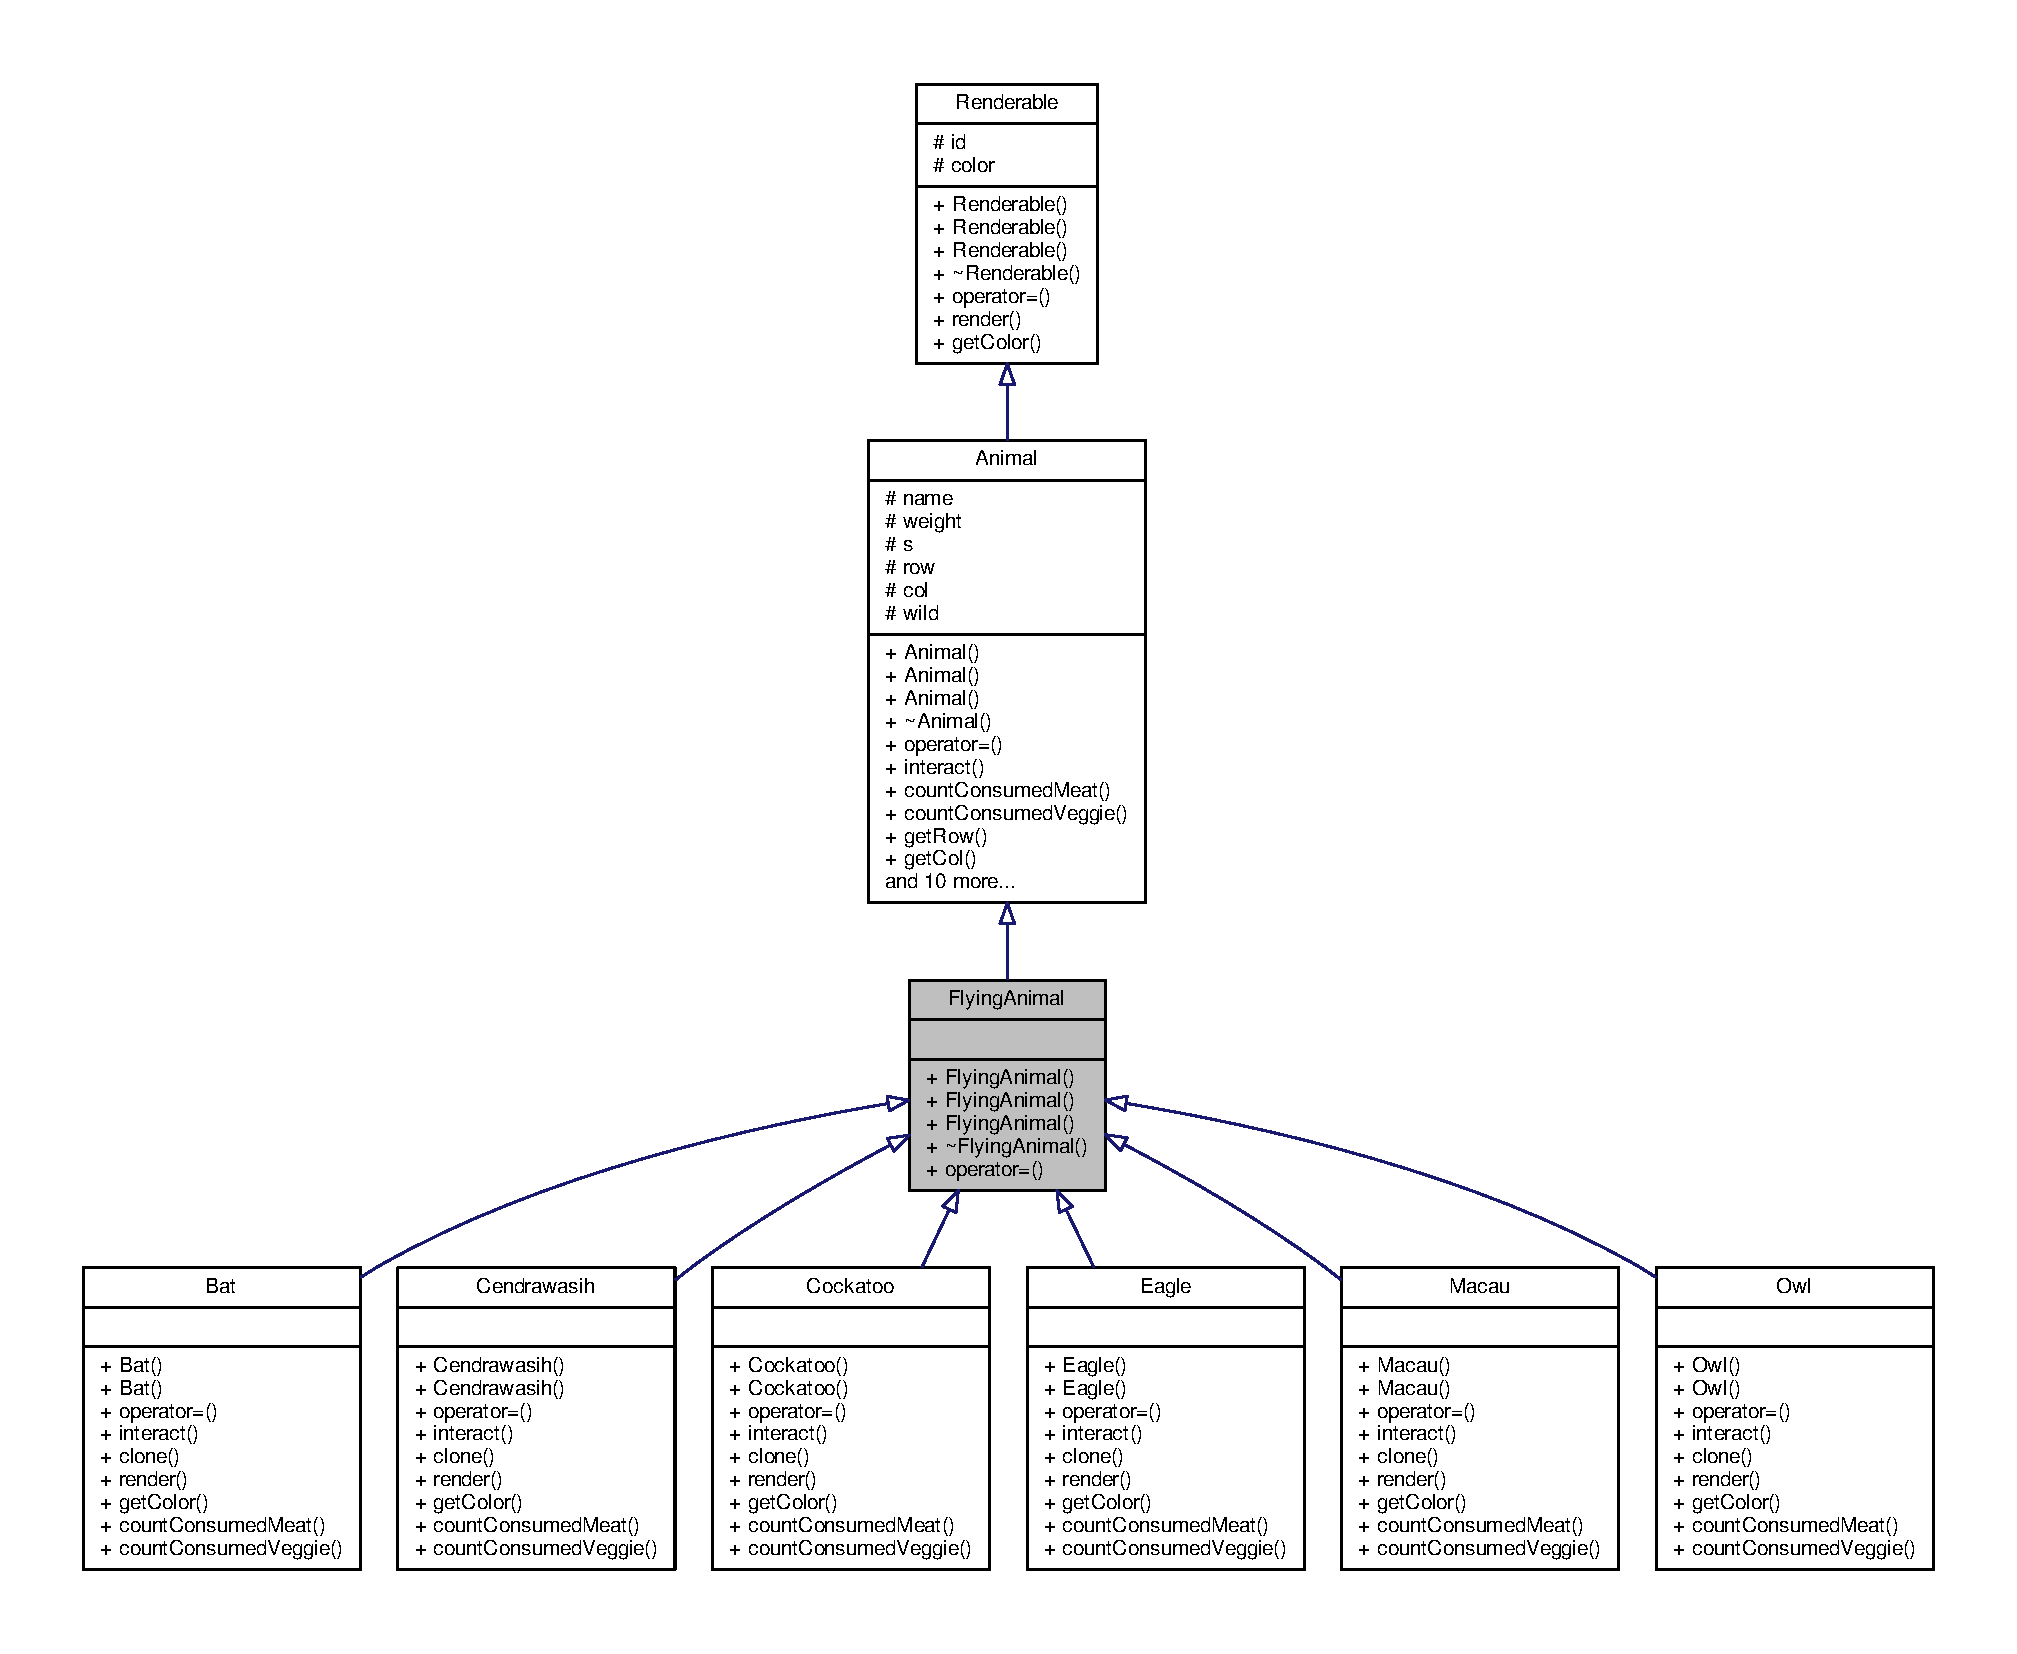
\includegraphics[width=350pt]{classFlyingAnimal__inherit__graph}
\end{center}
\end{figure}


Collaboration diagram for Flying\+Animal\+:
\nopagebreak
\begin{figure}[H]
\begin{center}
\leavevmode
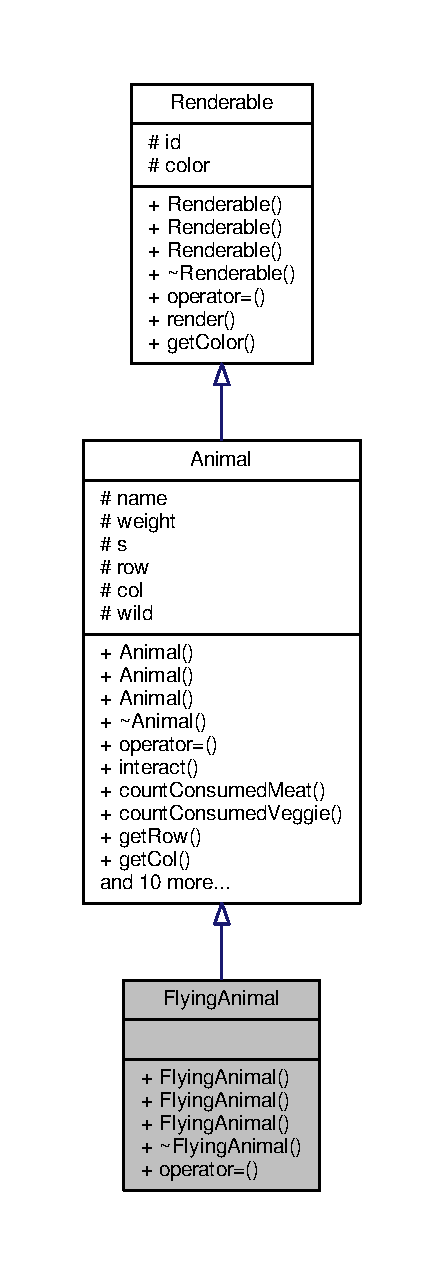
\includegraphics[height=550pt]{classFlyingAnimal__coll__graph}
\end{center}
\end{figure}
\subsection*{Public Member Functions}
\begin{DoxyCompactItemize}
\item 
\hyperlink{classFlyingAnimal_ab227c4204ac6c943f73ed58360d4d543}{Flying\+Animal} ()
\item 
\hyperlink{classFlyingAnimal_ad0a3cbbdb533fc87a5621a9af5db8280}{Flying\+Animal} (string \+\_\+name, double \+\_\+weight, \hyperlink{sex_8h_a2633cb393c68bb2ee8080db58fb7ba93}{Sex} \+\_\+s, int \+\_\+r, int \+\_\+c, char \+\_\+id, \hyperlink{color_8h_ab87bacfdad76e61b9412d7124be44c1c}{Color} \+\_\+color, bool \+\_\+w)
\begin{DoxyCompactList}\small\item\em Constructor. \end{DoxyCompactList}\item 
\hyperlink{classFlyingAnimal_ab2209a5b0286a65e2908a2fb7565e600}{Flying\+Animal} (const \hyperlink{classFlyingAnimal}{Flying\+Animal} \&)
\begin{DoxyCompactList}\small\item\em Copy Constructor. \end{DoxyCompactList}\item 
virtual \hyperlink{classFlyingAnimal_a50a93cfcb6d0f216032279f463347544}{$\sim$\+Flying\+Animal} ()
\begin{DoxyCompactList}\small\item\em Destructor. \end{DoxyCompactList}\item 
\hyperlink{classFlyingAnimal}{Flying\+Animal} \& \hyperlink{classFlyingAnimal_a7ec81003eaec2f95ab01419e373ee2b3}{operator=} (const \hyperlink{classFlyingAnimal}{Flying\+Animal} \&)
\begin{DoxyCompactList}\small\item\em Operator= Menjamin bukan bitwise copy. \end{DoxyCompactList}\end{DoxyCompactItemize}
\subsection*{Additional Inherited Members}


\subsection{Detailed Description}
Adalah kelas anak \hyperlink{classAnimal}{Animal}. Menggunakan virtual inheritance untuk menghindari ambiguitas karena diamond inheritance. 

\subsection{Constructor \& Destructor Documentation}
\index{Flying\+Animal@{Flying\+Animal}!Flying\+Animal@{Flying\+Animal}}
\index{Flying\+Animal@{Flying\+Animal}!Flying\+Animal@{Flying\+Animal}}
\subsubsection[{\texorpdfstring{Flying\+Animal()}{FlyingAnimal()}}]{\setlength{\rightskip}{0pt plus 5cm}Flying\+Animal\+::\+Flying\+Animal (
\begin{DoxyParamCaption}
{}
\end{DoxyParamCaption}
)}\hypertarget{classFlyingAnimal_ab227c4204ac6c943f73ed58360d4d543}{}\label{classFlyingAnimal_ab227c4204ac6c943f73ed58360d4d543}
\index{Flying\+Animal@{Flying\+Animal}!Flying\+Animal@{Flying\+Animal}}
\index{Flying\+Animal@{Flying\+Animal}!Flying\+Animal@{Flying\+Animal}}
\subsubsection[{\texorpdfstring{Flying\+Animal(string \+\_\+name, double \+\_\+weight, Sex \+\_\+s, int \+\_\+r, int \+\_\+c, char \+\_\+id, Color \+\_\+color, bool \+\_\+w)}{FlyingAnimal(string _name, double _weight, Sex _s, int _r, int _c, char _id, Color _color, bool _w)}}]{\setlength{\rightskip}{0pt plus 5cm}Flying\+Animal\+::\+Flying\+Animal (
\begin{DoxyParamCaption}
\item[{string}]{\+\_\+name, }
\item[{double}]{\+\_\+weight, }
\item[{{\bf Sex}}]{\+\_\+s, }
\item[{int}]{\+\_\+r, }
\item[{int}]{\+\_\+c, }
\item[{char}]{\+\_\+id, }
\item[{{\bf Color}}]{\+\_\+color, }
\item[{bool}]{\+\_\+w}
\end{DoxyParamCaption}
)}\hypertarget{classFlyingAnimal_ad0a3cbbdb533fc87a5621a9af5db8280}{}\label{classFlyingAnimal_ad0a3cbbdb533fc87a5621a9af5db8280}


Constructor. 

\index{Flying\+Animal@{Flying\+Animal}!Flying\+Animal@{Flying\+Animal}}
\index{Flying\+Animal@{Flying\+Animal}!Flying\+Animal@{Flying\+Animal}}
\subsubsection[{\texorpdfstring{Flying\+Animal(const Flying\+Animal \&)}{FlyingAnimal(const FlyingAnimal &)}}]{\setlength{\rightskip}{0pt plus 5cm}Flying\+Animal\+::\+Flying\+Animal (
\begin{DoxyParamCaption}
\item[{const {\bf Flying\+Animal} \&}]{F}
\end{DoxyParamCaption}
)}\hypertarget{classFlyingAnimal_ab2209a5b0286a65e2908a2fb7565e600}{}\label{classFlyingAnimal_ab2209a5b0286a65e2908a2fb7565e600}


Copy Constructor. 


\begin{DoxyParams}{Parameters}
{\em \hyperlink{classAnimal}{Animal}} & A yang ingin disalin. \\
\hline
\end{DoxyParams}
\index{Flying\+Animal@{Flying\+Animal}!````~Flying\+Animal@{$\sim$\+Flying\+Animal}}
\index{````~Flying\+Animal@{$\sim$\+Flying\+Animal}!Flying\+Animal@{Flying\+Animal}}
\subsubsection[{\texorpdfstring{$\sim$\+Flying\+Animal()}{~FlyingAnimal()}}]{\setlength{\rightskip}{0pt plus 5cm}Flying\+Animal\+::$\sim$\+Flying\+Animal (
\begin{DoxyParamCaption}
{}
\end{DoxyParamCaption}
)\hspace{0.3cm}{\ttfamily [virtual]}}\hypertarget{classFlyingAnimal_a50a93cfcb6d0f216032279f463347544}{}\label{classFlyingAnimal_a50a93cfcb6d0f216032279f463347544}


Destructor. 



\subsection{Member Function Documentation}
\index{Flying\+Animal@{Flying\+Animal}!operator=@{operator=}}
\index{operator=@{operator=}!Flying\+Animal@{Flying\+Animal}}
\subsubsection[{\texorpdfstring{operator=(const Flying\+Animal \&)}{operator=(const FlyingAnimal &)}}]{\setlength{\rightskip}{0pt plus 5cm}{\bf Flying\+Animal} \& Flying\+Animal\+::operator= (
\begin{DoxyParamCaption}
\item[{const {\bf Flying\+Animal} \&}]{F}
\end{DoxyParamCaption}
)}\hypertarget{classFlyingAnimal_a7ec81003eaec2f95ab01419e373ee2b3}{}\label{classFlyingAnimal_a7ec81003eaec2f95ab01419e373ee2b3}


Operator= Menjamin bukan bitwise copy. 

\begin{DoxyReturn}{Returns}
\hyperlink{classAnimal}{Animal} yang sudah di assign nilai dari current object. 
\end{DoxyReturn}


The documentation for this class was generated from the following files\+:\begin{DoxyCompactItemize}
\item 
src/renders/animals/\hyperlink{flying__animal_8h}{flying\+\_\+animal.\+h}\item 
src/renders/animals/\hyperlink{flying__animal_8cpp}{flying\+\_\+animal.\+cpp}\end{DoxyCompactItemize}

\hypertarget{classFrog}{}\section{Frog Class Reference}
\label{classFrog}\index{Frog@{Frog}}


{\ttfamily \#include $<$species.\+h$>$}



Inheritance diagram for Frog\+:
\nopagebreak
\begin{figure}[H]
\begin{center}
\leavevmode
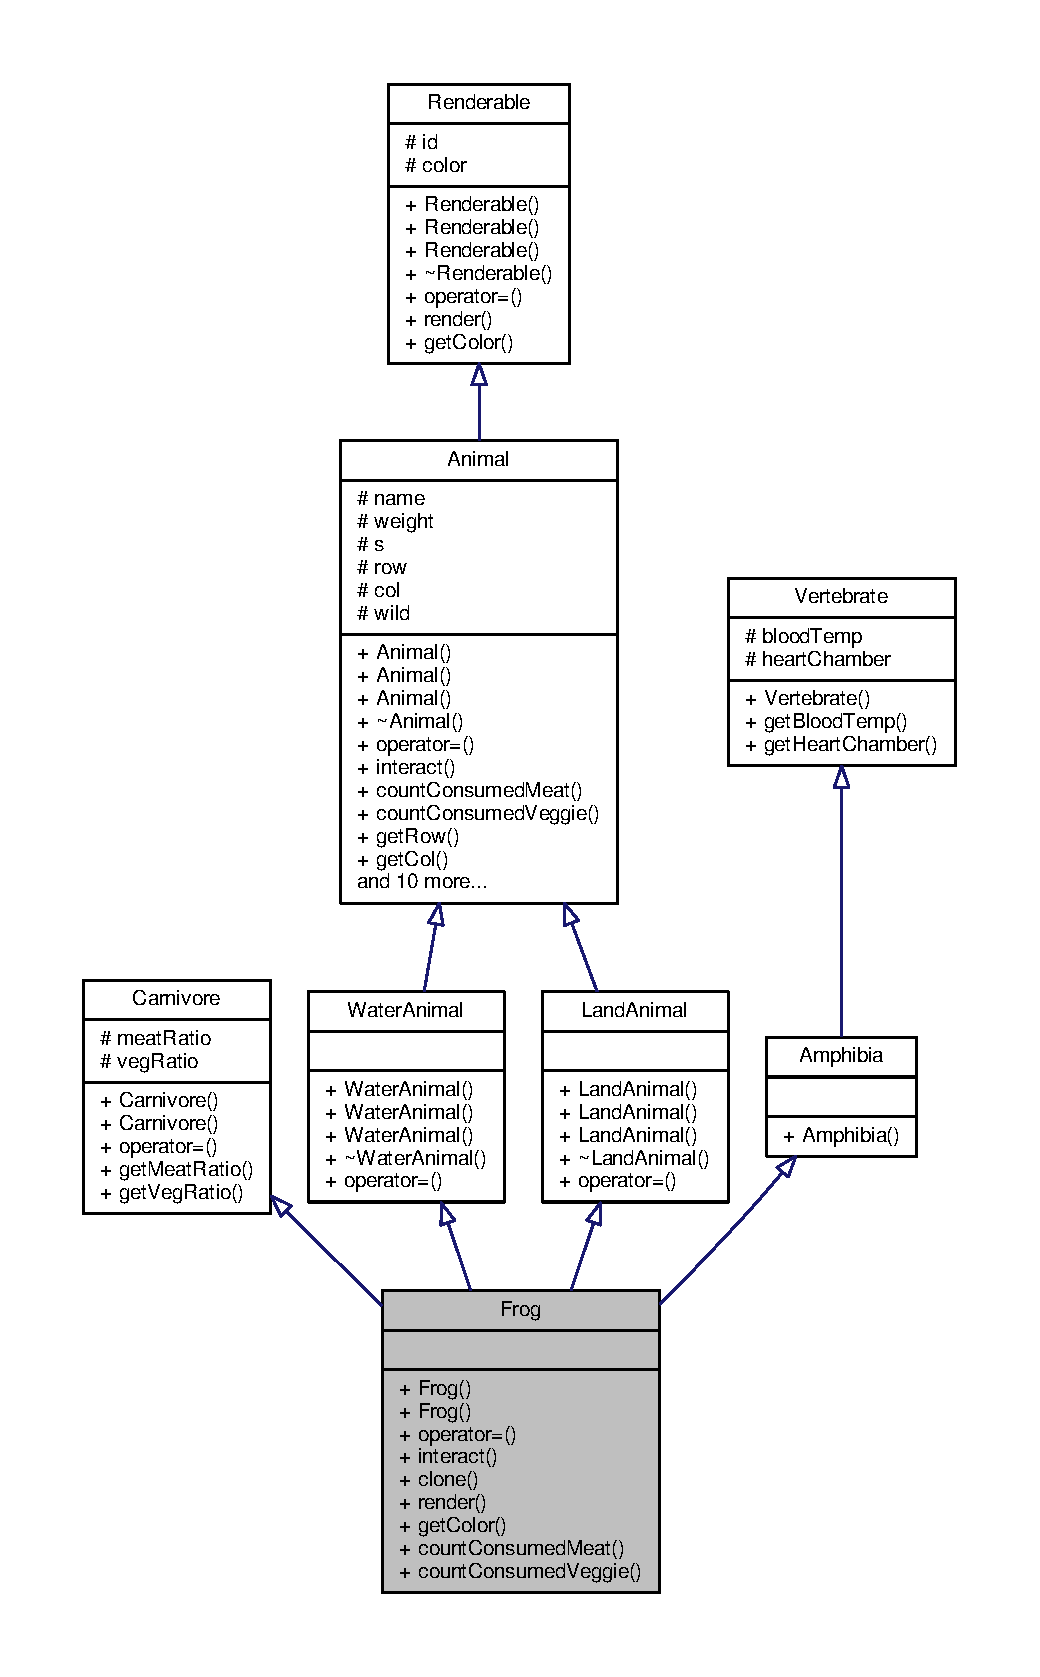
\includegraphics[height=550pt]{classFrog__inherit__graph}
\end{center}
\end{figure}


Collaboration diagram for Frog\+:
\nopagebreak
\begin{figure}[H]
\begin{center}
\leavevmode
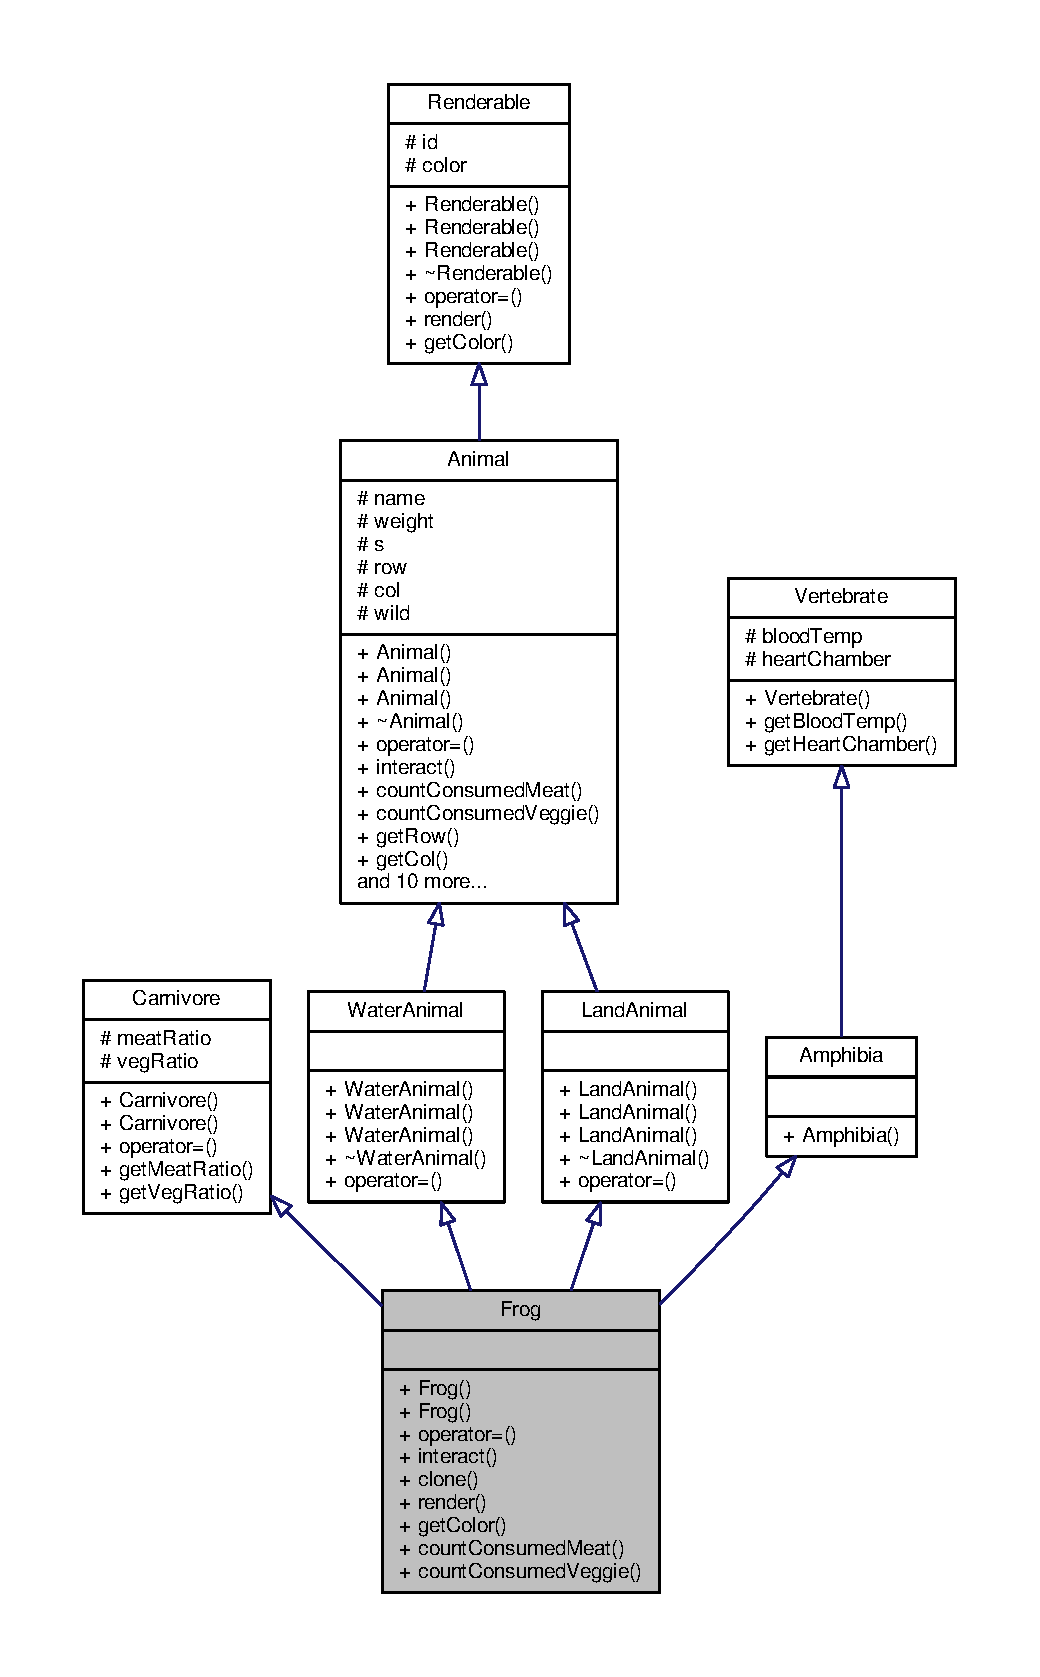
\includegraphics[height=550pt]{classFrog__coll__graph}
\end{center}
\end{figure}
\subsection*{Public Member Functions}
\begin{DoxyCompactItemize}
\item 
\hyperlink{classFrog_a9d2d178018dce67508988cfbee10a45b}{Frog} (string \+\_\+name, double \+\_\+weight, \hyperlink{sex_8h_a2633cb393c68bb2ee8080db58fb7ba93}{Sex} \+\_\+s, int \+\_\+r, int \+\_\+c)
\begin{DoxyCompactList}\small\item\em Consructor. \end{DoxyCompactList}\item 
\hyperlink{classFrog_ad799dd037bbf07877f47f512478f5971}{Frog} (const \hyperlink{classFrog}{Frog} \&F)
\begin{DoxyCompactList}\small\item\em Copy Consructor. \end{DoxyCompactList}\item 
\hyperlink{classFrog}{Frog} \& \hyperlink{classFrog_a6ae0b058647cf4fe8565f27029d1d02a}{operator=} (const \hyperlink{classFrog}{Frog} \&F)
\begin{DoxyCompactList}\small\item\em Operator=. Melakukan assignment pada objek. \end{DoxyCompactList}\item 
virtual void \hyperlink{classFrog_a1f48dff9c7eb100579f938c53c9fa25b}{interact} ()
\begin{DoxyCompactList}\small\item\em interact. Menampilkan interaksi hewan ke layar \end{DoxyCompactList}\item 
virtual \hyperlink{classFrog}{Frog} $\ast$ \hyperlink{classFrog_aab84684c4f6729ab89b1dd7470471d06}{clone} () const 
\begin{DoxyCompactList}\small\item\em clone Menduplikat diri sendiri \end{DoxyCompactList}\item 
virtual char \hyperlink{classFrog_a000e111ff655934cde3f06132841e736}{render} ()
\begin{DoxyCompactList}\small\item\em render Mengembalikan karakter id tiap hewan \end{DoxyCompactList}\item 
virtual \hyperlink{color_8h_ab87bacfdad76e61b9412d7124be44c1c}{Color} \hyperlink{classFrog_a6c7683144ff8beae2b66905178f74ed4}{get\+Color} ()
\begin{DoxyCompactList}\small\item\em get\+Color Mengembalikan warna dari hewan \end{DoxyCompactList}\item 
virtual double \hyperlink{classFrog_a5297e5e8eebab6d3f67c36e318db56fe}{count\+Consumed\+Meat} ()
\begin{DoxyCompactList}\small\item\em count\+Consumed\+Meat Mengembalikan jumlah daging yang dikonsumsi \end{DoxyCompactList}\item 
virtual double \hyperlink{classFrog_a0e6b1ee5d8a1dee1adde9ca4f3c7367e}{count\+Consumed\+Veggie} ()
\begin{DoxyCompactList}\small\item\em count\+Consumed\+Veggie Mengembalikan jumlah makanan tumbuhan yang dikonsumsi \end{DoxyCompactList}\end{DoxyCompactItemize}
\subsection*{Additional Inherited Members}


\subsection{Constructor \& Destructor Documentation}
\index{Frog@{Frog}!Frog@{Frog}}
\index{Frog@{Frog}!Frog@{Frog}}
\subsubsection[{\texorpdfstring{Frog(string \+\_\+name, double \+\_\+weight, Sex \+\_\+s, int \+\_\+r, int \+\_\+c)}{Frog(string _name, double _weight, Sex _s, int _r, int _c)}}]{\setlength{\rightskip}{0pt plus 5cm}Frog\+::\+Frog (
\begin{DoxyParamCaption}
\item[{string}]{\+\_\+name, }
\item[{double}]{\+\_\+weight, }
\item[{{\bf Sex}}]{\+\_\+s, }
\item[{int}]{\+\_\+r, }
\item[{int}]{\+\_\+c}
\end{DoxyParamCaption}
)}\hypertarget{classFrog_a9d2d178018dce67508988cfbee10a45b}{}\label{classFrog_a9d2d178018dce67508988cfbee10a45b}


Consructor. 


\begin{DoxyParams}{Parameters}
{\em \+\_\+name} & nama binatang \\
\hline
{\em \+\_\+weight} & berat \\
\hline
{\em \+\_\+s} & jenis kelamin \\
\hline
\end{DoxyParams}
\index{Frog@{Frog}!Frog@{Frog}}
\index{Frog@{Frog}!Frog@{Frog}}
\subsubsection[{\texorpdfstring{Frog(const Frog \&\+F)}{Frog(const Frog &F)}}]{\setlength{\rightskip}{0pt plus 5cm}Frog\+::\+Frog (
\begin{DoxyParamCaption}
\item[{const {\bf Frog} \&}]{F}
\end{DoxyParamCaption}
)}\hypertarget{classFrog_ad799dd037bbf07877f47f512478f5971}{}\label{classFrog_ad799dd037bbf07877f47f512478f5971}


Copy Consructor. 


\begin{DoxyParams}{Parameters}
{\em F} & objek yang akan disalin \\
\hline
\end{DoxyParams}


\subsection{Member Function Documentation}
\index{Frog@{Frog}!clone@{clone}}
\index{clone@{clone}!Frog@{Frog}}
\subsubsection[{\texorpdfstring{clone() const }{clone() const }}]{\setlength{\rightskip}{0pt plus 5cm}{\bf Frog} $\ast$ Frog\+::clone (
\begin{DoxyParamCaption}
{}
\end{DoxyParamCaption}
) const\hspace{0.3cm}{\ttfamily [virtual]}}\hypertarget{classFrog_aab84684c4f6729ab89b1dd7470471d06}{}\label{classFrog_aab84684c4f6729ab89b1dd7470471d06}


clone Menduplikat diri sendiri 

\begin{DoxyReturn}{Returns}
value object hasil kloning 
\end{DoxyReturn}


Implements \hyperlink{classAnimal_a1430e040ea4ff43bc453fa0ad19c308d}{Animal}.

\index{Frog@{Frog}!count\+Consumed\+Meat@{count\+Consumed\+Meat}}
\index{count\+Consumed\+Meat@{count\+Consumed\+Meat}!Frog@{Frog}}
\subsubsection[{\texorpdfstring{count\+Consumed\+Meat()}{countConsumedMeat()}}]{\setlength{\rightskip}{0pt plus 5cm}double Frog\+::count\+Consumed\+Meat (
\begin{DoxyParamCaption}
{}
\end{DoxyParamCaption}
)\hspace{0.3cm}{\ttfamily [virtual]}}\hypertarget{classFrog_a5297e5e8eebab6d3f67c36e318db56fe}{}\label{classFrog_a5297e5e8eebab6d3f67c36e318db56fe}


count\+Consumed\+Meat Mengembalikan jumlah daging yang dikonsumsi 

\begin{DoxyReturn}{Returns}
jumlah daging yang dikonsumsi 
\end{DoxyReturn}


Implements \hyperlink{classAnimal_a84ccc380d237650f2bf24d792627d376}{Animal}.

\index{Frog@{Frog}!count\+Consumed\+Veggie@{count\+Consumed\+Veggie}}
\index{count\+Consumed\+Veggie@{count\+Consumed\+Veggie}!Frog@{Frog}}
\subsubsection[{\texorpdfstring{count\+Consumed\+Veggie()}{countConsumedVeggie()}}]{\setlength{\rightskip}{0pt plus 5cm}double Frog\+::count\+Consumed\+Veggie (
\begin{DoxyParamCaption}
{}
\end{DoxyParamCaption}
)\hspace{0.3cm}{\ttfamily [virtual]}}\hypertarget{classFrog_a0e6b1ee5d8a1dee1adde9ca4f3c7367e}{}\label{classFrog_a0e6b1ee5d8a1dee1adde9ca4f3c7367e}


count\+Consumed\+Veggie Mengembalikan jumlah makanan tumbuhan yang dikonsumsi 

\begin{DoxyReturn}{Returns}
jumlah makanan tumbuhan yang dikonsumsi 
\end{DoxyReturn}


Implements \hyperlink{classAnimal_aaa7e4bdb7f5a10060b6dcaf09215f822}{Animal}.

\index{Frog@{Frog}!get\+Color@{get\+Color}}
\index{get\+Color@{get\+Color}!Frog@{Frog}}
\subsubsection[{\texorpdfstring{get\+Color()}{getColor()}}]{\setlength{\rightskip}{0pt plus 5cm}{\bf Color} Frog\+::get\+Color (
\begin{DoxyParamCaption}
{}
\end{DoxyParamCaption}
)\hspace{0.3cm}{\ttfamily [virtual]}}\hypertarget{classFrog_a6c7683144ff8beae2b66905178f74ed4}{}\label{classFrog_a6c7683144ff8beae2b66905178f74ed4}


get\+Color Mengembalikan warna dari hewan 

\begin{DoxyReturn}{Returns}
warna cetak hewan 
\end{DoxyReturn}


Implements \hyperlink{classRenderable_ab3bcc93b20929c6e92b64223344a73d5}{Renderable}.

\index{Frog@{Frog}!interact@{interact}}
\index{interact@{interact}!Frog@{Frog}}
\subsubsection[{\texorpdfstring{interact()}{interact()}}]{\setlength{\rightskip}{0pt plus 5cm}void Frog\+::interact (
\begin{DoxyParamCaption}
{}
\end{DoxyParamCaption}
)\hspace{0.3cm}{\ttfamily [virtual]}}\hypertarget{classFrog_a1f48dff9c7eb100579f938c53c9fa25b}{}\label{classFrog_a1f48dff9c7eb100579f938c53c9fa25b}


interact. Menampilkan interaksi hewan ke layar 



Implements \hyperlink{classAnimal_af47626b050b665e9a19525227d2b840f}{Animal}.

\index{Frog@{Frog}!operator=@{operator=}}
\index{operator=@{operator=}!Frog@{Frog}}
\subsubsection[{\texorpdfstring{operator=(const Frog \&\+F)}{operator=(const Frog &F)}}]{\setlength{\rightskip}{0pt plus 5cm}{\bf Frog} \& Frog\+::operator= (
\begin{DoxyParamCaption}
\item[{const {\bf Frog} \&}]{F}
\end{DoxyParamCaption}
)}\hypertarget{classFrog_a6ae0b058647cf4fe8565f27029d1d02a}{}\label{classFrog_a6ae0b058647cf4fe8565f27029d1d02a}


Operator=. Melakukan assignment pada objek. 


\begin{DoxyParams}{Parameters}
{\em F} & objek yang akan disalin \\
\hline
\end{DoxyParams}
\index{Frog@{Frog}!render@{render}}
\index{render@{render}!Frog@{Frog}}
\subsubsection[{\texorpdfstring{render()}{render()}}]{\setlength{\rightskip}{0pt plus 5cm}char Frog\+::render (
\begin{DoxyParamCaption}
{}
\end{DoxyParamCaption}
)\hspace{0.3cm}{\ttfamily [virtual]}}\hypertarget{classFrog_a000e111ff655934cde3f06132841e736}{}\label{classFrog_a000e111ff655934cde3f06132841e736}


render Mengembalikan karakter id tiap hewan 

\begin{DoxyReturn}{Returns}
karakter tiap hewan 
\end{DoxyReturn}


Implements \hyperlink{classRenderable_aafa9280e6dcfa557b3cd675221fd97b4}{Renderable}.



The documentation for this class was generated from the following files\+:\begin{DoxyCompactItemize}
\item 
src/renders/animals/\hyperlink{species_8h}{species.\+h}\item 
src/renders/animals/\hyperlink{species_8cpp}{species.\+cpp}\end{DoxyCompactItemize}

\hypertarget{classGiraffe}{}\section{Giraffe Class Reference}
\label{classGiraffe}\index{Giraffe@{Giraffe}}


{\ttfamily \#include $<$species.\+h$>$}



Inheritance diagram for Giraffe\+:
\nopagebreak
\begin{figure}[H]
\begin{center}
\leavevmode
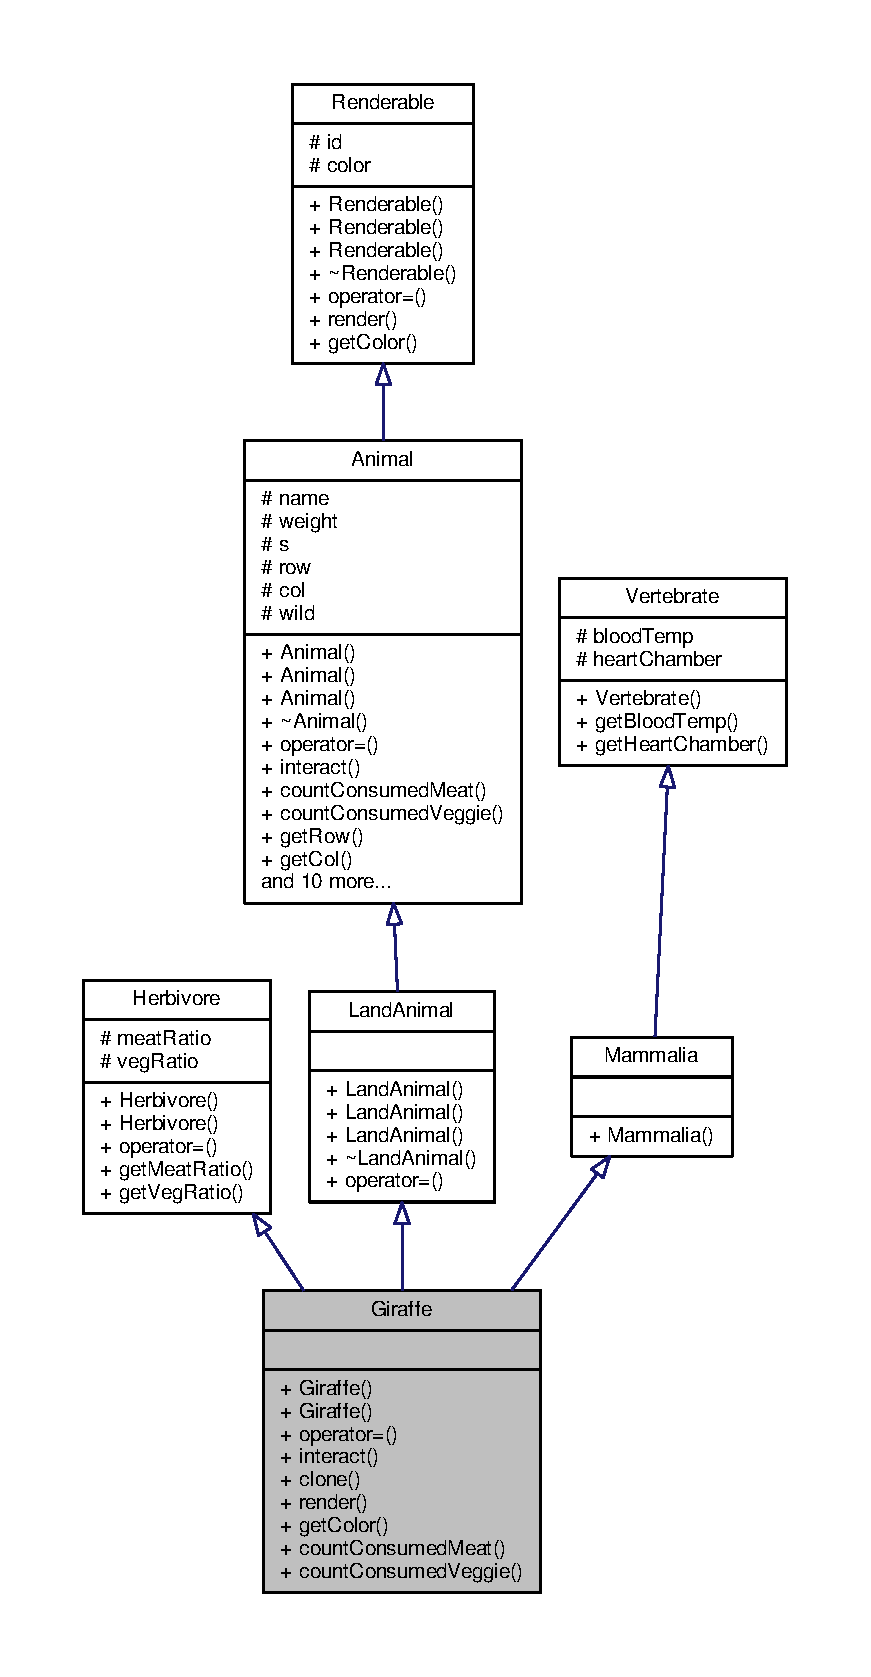
\includegraphics[height=550pt]{classGiraffe__inherit__graph}
\end{center}
\end{figure}


Collaboration diagram for Giraffe\+:
\nopagebreak
\begin{figure}[H]
\begin{center}
\leavevmode
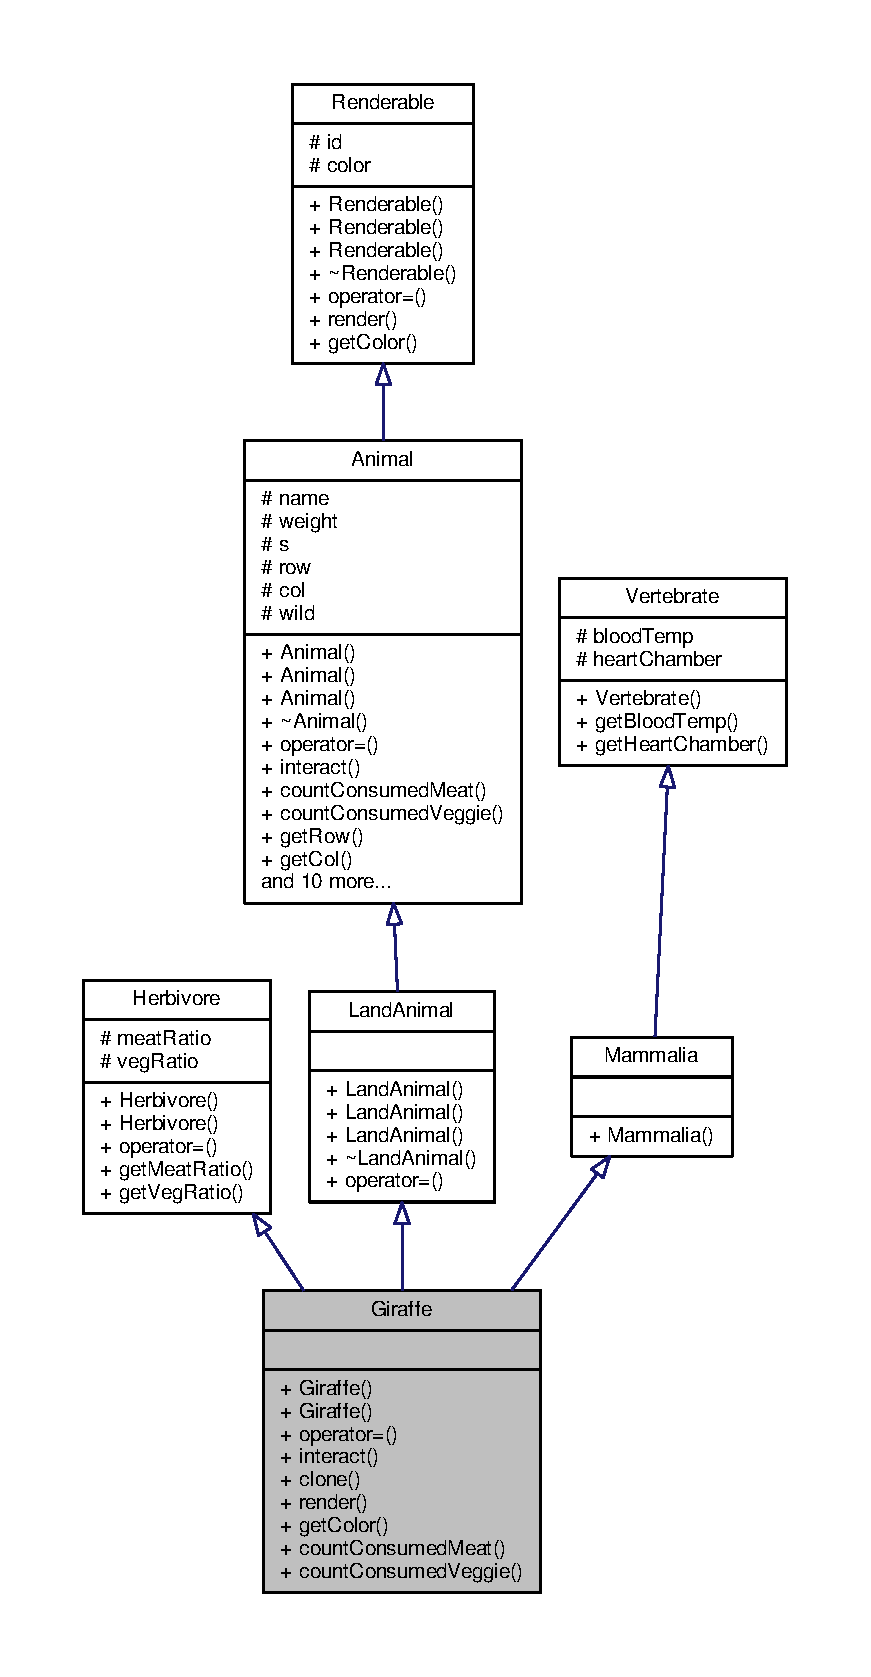
\includegraphics[height=550pt]{classGiraffe__coll__graph}
\end{center}
\end{figure}
\subsection*{Public Member Functions}
\begin{DoxyCompactItemize}
\item 
\hyperlink{classGiraffe_a9035d9accbc1aa1aba873b5f1ab7f350}{Giraffe} (string \+\_\+name, double \+\_\+weight, \hyperlink{sex_8h_a2633cb393c68bb2ee8080db58fb7ba93}{Sex} \+\_\+s, int \+\_\+r, int \+\_\+c)
\begin{DoxyCompactList}\small\item\em Consructor. \end{DoxyCompactList}\item 
\hyperlink{classGiraffe_ad0e9bb43e9f3ff379e21d70e6c9656ee}{Giraffe} (const \hyperlink{classGiraffe}{Giraffe} \&G)
\begin{DoxyCompactList}\small\item\em Copy Consructor. \end{DoxyCompactList}\item 
\hyperlink{classGiraffe}{Giraffe} \& \hyperlink{classGiraffe_a11f42a66f815b024ffa71f65934a1621}{operator=} (const \hyperlink{classGiraffe}{Giraffe} \&G)
\begin{DoxyCompactList}\small\item\em Operator=. Melakukan assignment pada objek. \end{DoxyCompactList}\item 
virtual void \hyperlink{classGiraffe_a70da7b25c32699f3b2a2bc85cd61b2e0}{interact} ()
\begin{DoxyCompactList}\small\item\em interact. Menampilkan interaksi hewan ke layar \end{DoxyCompactList}\item 
virtual \hyperlink{classGiraffe}{Giraffe} $\ast$ \hyperlink{classGiraffe_a37a4621ceb9515e1069a691971c4a31b}{clone} () const 
\begin{DoxyCompactList}\small\item\em clone Menduplikat diri sendiri \end{DoxyCompactList}\item 
virtual char \hyperlink{classGiraffe_a4dc522e81fb41129ecc73861180194ca}{render} ()
\begin{DoxyCompactList}\small\item\em render Mengembalikan karakter id tiap hewan \end{DoxyCompactList}\item 
virtual \hyperlink{color_8h_ab87bacfdad76e61b9412d7124be44c1c}{Color} \hyperlink{classGiraffe_a7ee9e17f63db1805a36a3d8ad209ef35}{get\+Color} ()
\begin{DoxyCompactList}\small\item\em get\+Color Mengembalikan warna dari hewan \end{DoxyCompactList}\item 
virtual double \hyperlink{classGiraffe_a18d770d4819d5c82ef9887a546765c89}{count\+Consumed\+Meat} ()
\begin{DoxyCompactList}\small\item\em count\+Consumed\+Meat Mengembalikan jumlah daging yang dikonsumsi \end{DoxyCompactList}\item 
virtual double \hyperlink{classGiraffe_ac998c481a5228750394bb8929174c618}{count\+Consumed\+Veggie} ()
\begin{DoxyCompactList}\small\item\em count\+Consumed\+Veggie Mengembalikan jumlah makanan tumbuhan yang dikonsumsi \end{DoxyCompactList}\end{DoxyCompactItemize}
\subsection*{Additional Inherited Members}


\subsection{Constructor \& Destructor Documentation}
\index{Giraffe@{Giraffe}!Giraffe@{Giraffe}}
\index{Giraffe@{Giraffe}!Giraffe@{Giraffe}}
\subsubsection[{\texorpdfstring{Giraffe(string \+\_\+name, double \+\_\+weight, Sex \+\_\+s, int \+\_\+r, int \+\_\+c)}{Giraffe(string _name, double _weight, Sex _s, int _r, int _c)}}]{\setlength{\rightskip}{0pt plus 5cm}Giraffe\+::\+Giraffe (
\begin{DoxyParamCaption}
\item[{string}]{\+\_\+name, }
\item[{double}]{\+\_\+weight, }
\item[{{\bf Sex}}]{\+\_\+s, }
\item[{int}]{\+\_\+r, }
\item[{int}]{\+\_\+c}
\end{DoxyParamCaption}
)}\hypertarget{classGiraffe_a9035d9accbc1aa1aba873b5f1ab7f350}{}\label{classGiraffe_a9035d9accbc1aa1aba873b5f1ab7f350}


Consructor. 


\begin{DoxyParams}{Parameters}
{\em \+\_\+name} & nama binatang \\
\hline
{\em \+\_\+weight} & berat \\
\hline
{\em \+\_\+s} & jenis kelamin \\
\hline
\end{DoxyParams}
\index{Giraffe@{Giraffe}!Giraffe@{Giraffe}}
\index{Giraffe@{Giraffe}!Giraffe@{Giraffe}}
\subsubsection[{\texorpdfstring{Giraffe(const Giraffe \&\+G)}{Giraffe(const Giraffe &G)}}]{\setlength{\rightskip}{0pt plus 5cm}Giraffe\+::\+Giraffe (
\begin{DoxyParamCaption}
\item[{const {\bf Giraffe} \&}]{G}
\end{DoxyParamCaption}
)}\hypertarget{classGiraffe_ad0e9bb43e9f3ff379e21d70e6c9656ee}{}\label{classGiraffe_ad0e9bb43e9f3ff379e21d70e6c9656ee}


Copy Consructor. 


\begin{DoxyParams}{Parameters}
{\em G} & objek yang akan disalin \\
\hline
\end{DoxyParams}


\subsection{Member Function Documentation}
\index{Giraffe@{Giraffe}!clone@{clone}}
\index{clone@{clone}!Giraffe@{Giraffe}}
\subsubsection[{\texorpdfstring{clone() const }{clone() const }}]{\setlength{\rightskip}{0pt plus 5cm}{\bf Giraffe} $\ast$ Giraffe\+::clone (
\begin{DoxyParamCaption}
{}
\end{DoxyParamCaption}
) const\hspace{0.3cm}{\ttfamily [virtual]}}\hypertarget{classGiraffe_a37a4621ceb9515e1069a691971c4a31b}{}\label{classGiraffe_a37a4621ceb9515e1069a691971c4a31b}


clone Menduplikat diri sendiri 

\begin{DoxyReturn}{Returns}
value object hasil kloning 
\end{DoxyReturn}


Implements \hyperlink{classAnimal_a1430e040ea4ff43bc453fa0ad19c308d}{Animal}.

\index{Giraffe@{Giraffe}!count\+Consumed\+Meat@{count\+Consumed\+Meat}}
\index{count\+Consumed\+Meat@{count\+Consumed\+Meat}!Giraffe@{Giraffe}}
\subsubsection[{\texorpdfstring{count\+Consumed\+Meat()}{countConsumedMeat()}}]{\setlength{\rightskip}{0pt plus 5cm}double Giraffe\+::count\+Consumed\+Meat (
\begin{DoxyParamCaption}
{}
\end{DoxyParamCaption}
)\hspace{0.3cm}{\ttfamily [virtual]}}\hypertarget{classGiraffe_a18d770d4819d5c82ef9887a546765c89}{}\label{classGiraffe_a18d770d4819d5c82ef9887a546765c89}


count\+Consumed\+Meat Mengembalikan jumlah daging yang dikonsumsi 

\begin{DoxyReturn}{Returns}
jumlah daging yang dikonsumsi 
\end{DoxyReturn}


Implements \hyperlink{classAnimal_a84ccc380d237650f2bf24d792627d376}{Animal}.

\index{Giraffe@{Giraffe}!count\+Consumed\+Veggie@{count\+Consumed\+Veggie}}
\index{count\+Consumed\+Veggie@{count\+Consumed\+Veggie}!Giraffe@{Giraffe}}
\subsubsection[{\texorpdfstring{count\+Consumed\+Veggie()}{countConsumedVeggie()}}]{\setlength{\rightskip}{0pt plus 5cm}double Giraffe\+::count\+Consumed\+Veggie (
\begin{DoxyParamCaption}
{}
\end{DoxyParamCaption}
)\hspace{0.3cm}{\ttfamily [virtual]}}\hypertarget{classGiraffe_ac998c481a5228750394bb8929174c618}{}\label{classGiraffe_ac998c481a5228750394bb8929174c618}


count\+Consumed\+Veggie Mengembalikan jumlah makanan tumbuhan yang dikonsumsi 

\begin{DoxyReturn}{Returns}
jumlah makanan tumbuhan yang dikonsumsi 
\end{DoxyReturn}


Implements \hyperlink{classAnimal_aaa7e4bdb7f5a10060b6dcaf09215f822}{Animal}.

\index{Giraffe@{Giraffe}!get\+Color@{get\+Color}}
\index{get\+Color@{get\+Color}!Giraffe@{Giraffe}}
\subsubsection[{\texorpdfstring{get\+Color()}{getColor()}}]{\setlength{\rightskip}{0pt plus 5cm}{\bf Color} Giraffe\+::get\+Color (
\begin{DoxyParamCaption}
{}
\end{DoxyParamCaption}
)\hspace{0.3cm}{\ttfamily [virtual]}}\hypertarget{classGiraffe_a7ee9e17f63db1805a36a3d8ad209ef35}{}\label{classGiraffe_a7ee9e17f63db1805a36a3d8ad209ef35}


get\+Color Mengembalikan warna dari hewan 

\begin{DoxyReturn}{Returns}
warna cetak hewan 
\end{DoxyReturn}


Implements \hyperlink{classRenderable_ab3bcc93b20929c6e92b64223344a73d5}{Renderable}.

\index{Giraffe@{Giraffe}!interact@{interact}}
\index{interact@{interact}!Giraffe@{Giraffe}}
\subsubsection[{\texorpdfstring{interact()}{interact()}}]{\setlength{\rightskip}{0pt plus 5cm}void Giraffe\+::interact (
\begin{DoxyParamCaption}
{}
\end{DoxyParamCaption}
)\hspace{0.3cm}{\ttfamily [virtual]}}\hypertarget{classGiraffe_a70da7b25c32699f3b2a2bc85cd61b2e0}{}\label{classGiraffe_a70da7b25c32699f3b2a2bc85cd61b2e0}


interact. Menampilkan interaksi hewan ke layar 



Implements \hyperlink{classAnimal_af47626b050b665e9a19525227d2b840f}{Animal}.

\index{Giraffe@{Giraffe}!operator=@{operator=}}
\index{operator=@{operator=}!Giraffe@{Giraffe}}
\subsubsection[{\texorpdfstring{operator=(const Giraffe \&\+G)}{operator=(const Giraffe &G)}}]{\setlength{\rightskip}{0pt plus 5cm}{\bf Giraffe} \& Giraffe\+::operator= (
\begin{DoxyParamCaption}
\item[{const {\bf Giraffe} \&}]{G}
\end{DoxyParamCaption}
)}\hypertarget{classGiraffe_a11f42a66f815b024ffa71f65934a1621}{}\label{classGiraffe_a11f42a66f815b024ffa71f65934a1621}


Operator=. Melakukan assignment pada objek. 


\begin{DoxyParams}{Parameters}
{\em G} & objek yang akan disalin \\
\hline
\end{DoxyParams}
\index{Giraffe@{Giraffe}!render@{render}}
\index{render@{render}!Giraffe@{Giraffe}}
\subsubsection[{\texorpdfstring{render()}{render()}}]{\setlength{\rightskip}{0pt plus 5cm}char Giraffe\+::render (
\begin{DoxyParamCaption}
{}
\end{DoxyParamCaption}
)\hspace{0.3cm}{\ttfamily [virtual]}}\hypertarget{classGiraffe_a4dc522e81fb41129ecc73861180194ca}{}\label{classGiraffe_a4dc522e81fb41129ecc73861180194ca}


render Mengembalikan karakter id tiap hewan 

\begin{DoxyReturn}{Returns}
karakter tiap hewan 
\end{DoxyReturn}


Implements \hyperlink{classRenderable_aafa9280e6dcfa557b3cd675221fd97b4}{Renderable}.



The documentation for this class was generated from the following files\+:\begin{DoxyCompactItemize}
\item 
src/renders/animals/\hyperlink{species_8h}{species.\+h}\item 
src/renders/animals/\hyperlink{species_8cpp}{species.\+cpp}\end{DoxyCompactItemize}

\hypertarget{classHabitat}{}\section{Habitat Class Reference}
\label{classHabitat}\index{Habitat@{Habitat}}


{\ttfamily \#include $<$habitat.\+h$>$}



Inheritance diagram for Habitat\+:
\nopagebreak
\begin{figure}[H]
\begin{center}
\leavevmode
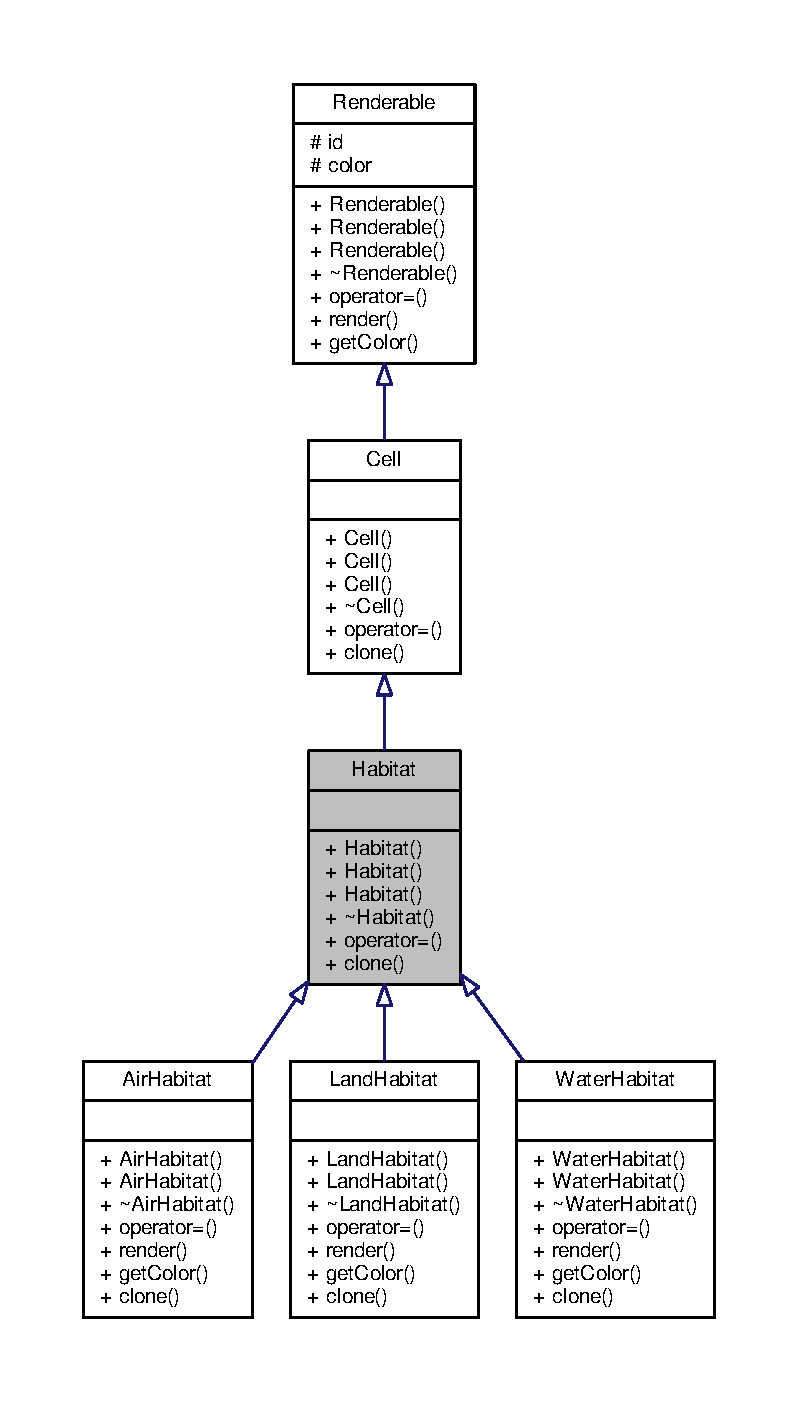
\includegraphics[height=550pt]{classHabitat__inherit__graph}
\end{center}
\end{figure}


Collaboration diagram for Habitat\+:
\nopagebreak
\begin{figure}[H]
\begin{center}
\leavevmode
\includegraphics[width=167pt]{classHabitat__coll__graph}
\end{center}
\end{figure}
\subsection*{Public Member Functions}
\begin{DoxyCompactItemize}
\item 
\hyperlink{classHabitat_ae46edb2802c122c0e7c8126e5895bf00}{Habitat} ()
\begin{DoxyCompactList}\small\item\em Constructor. Menciptakan \hyperlink{classHabitat}{Habitat} kosong. \end{DoxyCompactList}\item 
\hyperlink{classHabitat_ae3f26bd17b681c00eabb2cb4c8b2daba}{Habitat} (char \+\_\+id, \hyperlink{color_8h_ab87bacfdad76e61b9412d7124be44c1c}{Color} \+\_\+color)
\begin{DoxyCompactList}\small\item\em Constructor dengan parameter. Menciptakan \hyperlink{classHabitat}{Habitat} dengan parameter id dan color. \end{DoxyCompactList}\item 
\hyperlink{classHabitat_afde9178e3f2467ca26d0a8ff5af30a18}{Habitat} (const \hyperlink{classHabitat}{Habitat} \&)
\begin{DoxyCompactList}\small\item\em Copy Constructor. Menciptakan salinan dari \hyperlink{classHabitat}{Habitat}. \end{DoxyCompactList}\item 
virtual \hyperlink{classHabitat_afd413e46df54891b04262872f04b314f}{$\sim$\+Habitat} ()
\begin{DoxyCompactList}\small\item\em Destructor. \end{DoxyCompactList}\item 
\hyperlink{classHabitat}{Habitat} \& \hyperlink{classHabitat_a5469dca43cea4ace30c056b40f3371ef}{operator=} (const \hyperlink{classHabitat}{Habitat} \&)
\begin{DoxyCompactList}\small\item\em Operator=. Menginisialisasi \hyperlink{classHabitat}{Habitat} tanpa terjadi bitwise copy. \end{DoxyCompactList}\item 
virtual \hyperlink{classHabitat}{Habitat} $\ast$ \hyperlink{classHabitat_a640c071c99dbd3dc9cbf4971dbcaa463}{clone} () const =0
\begin{DoxyCompactList}\small\item\em clone. Menduplikasi \hyperlink{classHabitat}{Habitat} tanpa terjadi bitwise copy \end{DoxyCompactList}\end{DoxyCompactItemize}
\subsection*{Additional Inherited Members}


\subsection{Constructor \& Destructor Documentation}
\index{Habitat@{Habitat}!Habitat@{Habitat}}
\index{Habitat@{Habitat}!Habitat@{Habitat}}
\subsubsection[{\texorpdfstring{Habitat()}{Habitat()}}]{\setlength{\rightskip}{0pt plus 5cm}Habitat\+::\+Habitat (
\begin{DoxyParamCaption}
{}
\end{DoxyParamCaption}
)}\hypertarget{classHabitat_ae46edb2802c122c0e7c8126e5895bf00}{}\label{classHabitat_ae46edb2802c122c0e7c8126e5895bf00}


Constructor. Menciptakan \hyperlink{classHabitat}{Habitat} kosong. 

\index{Habitat@{Habitat}!Habitat@{Habitat}}
\index{Habitat@{Habitat}!Habitat@{Habitat}}
\subsubsection[{\texorpdfstring{Habitat(char \+\_\+id, Color \+\_\+color)}{Habitat(char _id, Color _color)}}]{\setlength{\rightskip}{0pt plus 5cm}Habitat\+::\+Habitat (
\begin{DoxyParamCaption}
\item[{char}]{\+\_\+id, }
\item[{{\bf Color}}]{\+\_\+color}
\end{DoxyParamCaption}
)}\hypertarget{classHabitat_ae3f26bd17b681c00eabb2cb4c8b2daba}{}\label{classHabitat_ae3f26bd17b681c00eabb2cb4c8b2daba}


Constructor dengan parameter. Menciptakan \hyperlink{classHabitat}{Habitat} dengan parameter id dan color. 


\begin{DoxyParams}{Parameters}
{\em id} & char renderable \\
\hline
{\em color} & warna renderable \\
\hline
\end{DoxyParams}
\index{Habitat@{Habitat}!Habitat@{Habitat}}
\index{Habitat@{Habitat}!Habitat@{Habitat}}
\subsubsection[{\texorpdfstring{Habitat(const Habitat \&)}{Habitat(const Habitat &)}}]{\setlength{\rightskip}{0pt plus 5cm}Habitat\+::\+Habitat (
\begin{DoxyParamCaption}
\item[{const {\bf Habitat} \&}]{H}
\end{DoxyParamCaption}
)}\hypertarget{classHabitat_afde9178e3f2467ca26d0a8ff5af30a18}{}\label{classHabitat_afde9178e3f2467ca26d0a8ff5af30a18}


Copy Constructor. Menciptakan salinan dari \hyperlink{classHabitat}{Habitat}. 


\begin{DoxyParams}{Parameters}
{\em H} & \hyperlink{classHabitat}{Habitat} yang ingin disalin. \\
\hline
\end{DoxyParams}
\index{Habitat@{Habitat}!````~Habitat@{$\sim$\+Habitat}}
\index{````~Habitat@{$\sim$\+Habitat}!Habitat@{Habitat}}
\subsubsection[{\texorpdfstring{$\sim$\+Habitat()}{~Habitat()}}]{\setlength{\rightskip}{0pt plus 5cm}Habitat\+::$\sim$\+Habitat (
\begin{DoxyParamCaption}
{}
\end{DoxyParamCaption}
)\hspace{0.3cm}{\ttfamily [virtual]}}\hypertarget{classHabitat_afd413e46df54891b04262872f04b314f}{}\label{classHabitat_afd413e46df54891b04262872f04b314f}


Destructor. 



\subsection{Member Function Documentation}
\index{Habitat@{Habitat}!clone@{clone}}
\index{clone@{clone}!Habitat@{Habitat}}
\subsubsection[{\texorpdfstring{clone() const =0}{clone() const =0}}]{\setlength{\rightskip}{0pt plus 5cm}virtual {\bf Habitat}$\ast$ Habitat\+::clone (
\begin{DoxyParamCaption}
{}
\end{DoxyParamCaption}
) const\hspace{0.3cm}{\ttfamily [pure virtual]}}\hypertarget{classHabitat_a640c071c99dbd3dc9cbf4971dbcaa463}{}\label{classHabitat_a640c071c99dbd3dc9cbf4971dbcaa463}


clone. Menduplikasi \hyperlink{classHabitat}{Habitat} tanpa terjadi bitwise copy 

\begin{DoxyReturn}{Returns}
\hyperlink{classHabitat}{Habitat} yang sudah diduplikasi. 
\end{DoxyReturn}


Implements \hyperlink{classCell_aafd03896d9a6131f14273752f9fb9815}{Cell}.



Implemented in \hyperlink{classAirHabitat_ab756521fcd5adca0283e9bfd0d0fd075}{Air\+Habitat}, \hyperlink{classLandHabitat_add986b725e19b857d3e3fa66689cda73}{Land\+Habitat}, and \hyperlink{classWaterHabitat_ab55d7a09373090cfafac504bc1431878}{Water\+Habitat}.

\index{Habitat@{Habitat}!operator=@{operator=}}
\index{operator=@{operator=}!Habitat@{Habitat}}
\subsubsection[{\texorpdfstring{operator=(const Habitat \&)}{operator=(const Habitat &)}}]{\setlength{\rightskip}{0pt plus 5cm}{\bf Habitat} \& Habitat\+::operator= (
\begin{DoxyParamCaption}
\item[{const {\bf Habitat} \&}]{H}
\end{DoxyParamCaption}
)}\hypertarget{classHabitat_a5469dca43cea4ace30c056b40f3371ef}{}\label{classHabitat_a5469dca43cea4ace30c056b40f3371ef}


Operator=. Menginisialisasi \hyperlink{classHabitat}{Habitat} tanpa terjadi bitwise copy. 

\begin{DoxyReturn}{Returns}
\hyperlink{classHabitat}{Habitat} yang sudah di assign nilai dari current object 
\end{DoxyReturn}


The documentation for this class was generated from the following files\+:\begin{DoxyCompactItemize}
\item 
src/renders/habitats/\hyperlink{habitat_8h}{habitat.\+h}\item 
src/renders/habitats/\hyperlink{habitat_8cpp}{habitat.\+cpp}\end{DoxyCompactItemize}

\hypertarget{classHerbivore}{}\section{Herbivore Class Reference}
\label{classHerbivore}\index{Herbivore@{Herbivore}}


{\ttfamily \#include $<$herbivore.\+h$>$}



Inheritance diagram for Herbivore\+:
\nopagebreak
\begin{figure}[H]
\begin{center}
\leavevmode
\includegraphics[width=350pt]{classHerbivore__inherit__graph}
\end{center}
\end{figure}


Collaboration diagram for Herbivore\+:
\nopagebreak
\begin{figure}[H]
\begin{center}
\leavevmode
\includegraphics[width=170pt]{classHerbivore__coll__graph}
\end{center}
\end{figure}
\subsection*{Public Member Functions}
\begin{DoxyCompactItemize}
\item 
\hyperlink{classHerbivore_aeed0ccda0f35ecc74f56a7ea21aa5286}{Herbivore} ()
\begin{DoxyCompactList}\small\item\em Constructor. \end{DoxyCompactList}\item 
\hyperlink{classHerbivore_a8158d0b440b52ed984c444367ef7990d}{Herbivore} (const \hyperlink{classHerbivore}{Herbivore} \&H)
\begin{DoxyCompactList}\small\item\em Copy Constructor. \end{DoxyCompactList}\item 
\hyperlink{classHerbivore}{Herbivore} \& \hyperlink{classHerbivore_a8c5a037a616f3475696e6984f1a60545}{operator=} (const \hyperlink{classHerbivore}{Herbivore} \&H)
\begin{DoxyCompactList}\small\item\em Operator=. Menjamin bukan bitwise copy. \end{DoxyCompactList}\item 
double \hyperlink{classHerbivore_a4c381eb2420800585b927caf008c48d8}{get\+Meat\+Ratio} () const 
\begin{DoxyCompactList}\small\item\em Getter. Mengembalikan nilai rasio daging. \end{DoxyCompactList}\item 
double \hyperlink{classHerbivore_aed86c22a9551c7ad0aab5488e6db6c94}{get\+Veg\+Ratio} () const 
\begin{DoxyCompactList}\small\item\em Getter. Mengembalikan nilai rasio daging. \end{DoxyCompactList}\end{DoxyCompactItemize}
\subsection*{Protected Attributes}
\begin{DoxyCompactItemize}
\item 
const double \hyperlink{classHerbivore_afc971698b03df63c433e8e6300f43347}{meat\+Ratio} = 0
\item 
double \hyperlink{classHerbivore_a4d0aec1023006ba35707eb15b7092360}{veg\+Ratio}
\end{DoxyCompactItemize}


\subsection{Detailed Description}
Kelas untuk hewan herbivora (pemakan tanaman) 

\subsection{Constructor \& Destructor Documentation}
\index{Herbivore@{Herbivore}!Herbivore@{Herbivore}}
\index{Herbivore@{Herbivore}!Herbivore@{Herbivore}}
\subsubsection[{\texorpdfstring{Herbivore()}{Herbivore()}}]{\setlength{\rightskip}{0pt plus 5cm}Herbivore\+::\+Herbivore (
\begin{DoxyParamCaption}
{}
\end{DoxyParamCaption}
)}\hypertarget{classHerbivore_aeed0ccda0f35ecc74f56a7ea21aa5286}{}\label{classHerbivore_aeed0ccda0f35ecc74f56a7ea21aa5286}


Constructor. 

\index{Herbivore@{Herbivore}!Herbivore@{Herbivore}}
\index{Herbivore@{Herbivore}!Herbivore@{Herbivore}}
\subsubsection[{\texorpdfstring{Herbivore(const Herbivore \&\+H)}{Herbivore(const Herbivore &H)}}]{\setlength{\rightskip}{0pt plus 5cm}Herbivore\+::\+Herbivore (
\begin{DoxyParamCaption}
\item[{const {\bf Herbivore} \&}]{H}
\end{DoxyParamCaption}
)}\hypertarget{classHerbivore_a8158d0b440b52ed984c444367ef7990d}{}\label{classHerbivore_a8158d0b440b52ed984c444367ef7990d}


Copy Constructor. 


\begin{DoxyParams}{Parameters}
{\em \hyperlink{classHerbivore}{Herbivore}} & H yang diacu cctor \\
\hline
\end{DoxyParams}


\subsection{Member Function Documentation}
\index{Herbivore@{Herbivore}!get\+Meat\+Ratio@{get\+Meat\+Ratio}}
\index{get\+Meat\+Ratio@{get\+Meat\+Ratio}!Herbivore@{Herbivore}}
\subsubsection[{\texorpdfstring{get\+Meat\+Ratio() const }{getMeatRatio() const }}]{\setlength{\rightskip}{0pt plus 5cm}double Herbivore\+::get\+Meat\+Ratio (
\begin{DoxyParamCaption}
{}
\end{DoxyParamCaption}
) const}\hypertarget{classHerbivore_a4c381eb2420800585b927caf008c48d8}{}\label{classHerbivore_a4c381eb2420800585b927caf008c48d8}


Getter. Mengembalikan nilai rasio daging. 

\begin{DoxyReturn}{Returns}
nilai rasio daging 
\end{DoxyReturn}
\index{Herbivore@{Herbivore}!get\+Veg\+Ratio@{get\+Veg\+Ratio}}
\index{get\+Veg\+Ratio@{get\+Veg\+Ratio}!Herbivore@{Herbivore}}
\subsubsection[{\texorpdfstring{get\+Veg\+Ratio() const }{getVegRatio() const }}]{\setlength{\rightskip}{0pt plus 5cm}double Herbivore\+::get\+Veg\+Ratio (
\begin{DoxyParamCaption}
{}
\end{DoxyParamCaption}
) const}\hypertarget{classHerbivore_aed86c22a9551c7ad0aab5488e6db6c94}{}\label{classHerbivore_aed86c22a9551c7ad0aab5488e6db6c94}


Getter. Mengembalikan nilai rasio daging. 

\begin{DoxyReturn}{Returns}
nilai rasio sayur 
\end{DoxyReturn}
\index{Herbivore@{Herbivore}!operator=@{operator=}}
\index{operator=@{operator=}!Herbivore@{Herbivore}}
\subsubsection[{\texorpdfstring{operator=(const Herbivore \&\+H)}{operator=(const Herbivore &H)}}]{\setlength{\rightskip}{0pt plus 5cm}{\bf Herbivore} \& Herbivore\+::operator= (
\begin{DoxyParamCaption}
\item[{const {\bf Herbivore} \&}]{H}
\end{DoxyParamCaption}
)}\hypertarget{classHerbivore_a8c5a037a616f3475696e6984f1a60545}{}\label{classHerbivore_a8c5a037a616f3475696e6984f1a60545}


Operator=. Menjamin bukan bitwise copy. 


\begin{DoxyParams}{Parameters}
{\em \hyperlink{classHerbivore}{Herbivore}} & H berisi data untuk diassign \\
\hline
\end{DoxyParams}


\subsection{Member Data Documentation}
\index{Herbivore@{Herbivore}!meat\+Ratio@{meat\+Ratio}}
\index{meat\+Ratio@{meat\+Ratio}!Herbivore@{Herbivore}}
\subsubsection[{\texorpdfstring{meat\+Ratio}{meatRatio}}]{\setlength{\rightskip}{0pt plus 5cm}const double Herbivore\+::meat\+Ratio = 0\hspace{0.3cm}{\ttfamily [protected]}}\hypertarget{classHerbivore_afc971698b03df63c433e8e6300f43347}{}\label{classHerbivore_afc971698b03df63c433e8e6300f43347}
\index{Herbivore@{Herbivore}!veg\+Ratio@{veg\+Ratio}}
\index{veg\+Ratio@{veg\+Ratio}!Herbivore@{Herbivore}}
\subsubsection[{\texorpdfstring{veg\+Ratio}{vegRatio}}]{\setlength{\rightskip}{0pt plus 5cm}double Herbivore\+::veg\+Ratio\hspace{0.3cm}{\ttfamily [protected]}}\hypertarget{classHerbivore_a4d0aec1023006ba35707eb15b7092360}{}\label{classHerbivore_a4d0aec1023006ba35707eb15b7092360}


The documentation for this class was generated from the following files\+:\begin{DoxyCompactItemize}
\item 
src/renders/animals/diet/\hyperlink{herbivore_8h}{herbivore.\+h}\item 
src/renders/animals/diet/\hyperlink{herbivore_8cpp}{herbivore.\+cpp}\end{DoxyCompactItemize}

\hypertarget{classHippopotamus}{}\section{Hippopotamus Class Reference}
\label{classHippopotamus}\index{Hippopotamus@{Hippopotamus}}


{\ttfamily \#include $<$species.\+h$>$}



Inheritance diagram for Hippopotamus\+:
\nopagebreak
\begin{figure}[H]
\begin{center}
\leavevmode
\includegraphics[height=550pt]{classHippopotamus__inherit__graph}
\end{center}
\end{figure}


Collaboration diagram for Hippopotamus\+:
\nopagebreak
\begin{figure}[H]
\begin{center}
\leavevmode
\includegraphics[height=550pt]{classHippopotamus__coll__graph}
\end{center}
\end{figure}
\subsection*{Public Member Functions}
\begin{DoxyCompactItemize}
\item 
\hyperlink{classHippopotamus_a2720f3349f57891bdd17c77b175b80a0}{Hippopotamus} (string \+\_\+name, double \+\_\+weight, \hyperlink{sex_8h_a2633cb393c68bb2ee8080db58fb7ba93}{Sex} \+\_\+s, int \+\_\+r, int \+\_\+c)
\begin{DoxyCompactList}\small\item\em Consructor. \end{DoxyCompactList}\item 
\hyperlink{classHippopotamus_a886733b750749ccf280d92cf14f1663e}{Hippopotamus} (const \hyperlink{classHippopotamus}{Hippopotamus} \&H)
\begin{DoxyCompactList}\small\item\em Copy Consructor. \end{DoxyCompactList}\item 
\hyperlink{classHippopotamus}{Hippopotamus} \& \hyperlink{classHippopotamus_ac6100e48b9175195a62f9652db5d7ce0}{operator=} (const \hyperlink{classHippopotamus}{Hippopotamus} \&H)
\begin{DoxyCompactList}\small\item\em Operator=. Melakukan assignment pada objek. \end{DoxyCompactList}\item 
virtual void \hyperlink{classHippopotamus_a36896f7daf07dbdf68153f371c2e5890}{interact} ()
\begin{DoxyCompactList}\small\item\em interact. Menampilkan interaksi hewan ke layar \end{DoxyCompactList}\item 
virtual \hyperlink{classHippopotamus}{Hippopotamus} $\ast$ \hyperlink{classHippopotamus_ae332973578e7a9a8bfde9cd7fb972d5e}{clone} () const 
\begin{DoxyCompactList}\small\item\em clone Menduplikat diri sendiri \end{DoxyCompactList}\item 
virtual char \hyperlink{classHippopotamus_a55c661408859ea2b5225931592b6d8e4}{render} ()
\begin{DoxyCompactList}\small\item\em render Mengembalikan karakter id tiap hewan \end{DoxyCompactList}\item 
virtual \hyperlink{color_8h_ab87bacfdad76e61b9412d7124be44c1c}{Color} \hyperlink{classHippopotamus_af719f3803c831533fa2709a9e6c8d015}{get\+Color} ()
\begin{DoxyCompactList}\small\item\em get\+Color Mengembalikan warna dari hewan \end{DoxyCompactList}\item 
virtual double \hyperlink{classHippopotamus_a55db3d0400a34c50b9dbf8718d31980c}{count\+Consumed\+Meat} ()
\begin{DoxyCompactList}\small\item\em count\+Consumed\+Meat Mengembalikan jumlah daging yang dikonsumsi \end{DoxyCompactList}\item 
virtual double \hyperlink{classHippopotamus_abf66ac77f92d82a60b76424e25fdd2fe}{count\+Consumed\+Veggie} ()
\begin{DoxyCompactList}\small\item\em count\+Consumed\+Veggie Mengembalikan jumlah makanan tumbuhan yang dikonsumsi \end{DoxyCompactList}\end{DoxyCompactItemize}
\subsection*{Additional Inherited Members}


\subsection{Constructor \& Destructor Documentation}
\index{Hippopotamus@{Hippopotamus}!Hippopotamus@{Hippopotamus}}
\index{Hippopotamus@{Hippopotamus}!Hippopotamus@{Hippopotamus}}
\subsubsection[{\texorpdfstring{Hippopotamus(string \+\_\+name, double \+\_\+weight, Sex \+\_\+s, int \+\_\+r, int \+\_\+c)}{Hippopotamus(string _name, double _weight, Sex _s, int _r, int _c)}}]{\setlength{\rightskip}{0pt plus 5cm}Hippopotamus\+::\+Hippopotamus (
\begin{DoxyParamCaption}
\item[{string}]{\+\_\+name, }
\item[{double}]{\+\_\+weight, }
\item[{{\bf Sex}}]{\+\_\+s, }
\item[{int}]{\+\_\+r, }
\item[{int}]{\+\_\+c}
\end{DoxyParamCaption}
)}\hypertarget{classHippopotamus_a2720f3349f57891bdd17c77b175b80a0}{}\label{classHippopotamus_a2720f3349f57891bdd17c77b175b80a0}


Consructor. 


\begin{DoxyParams}{Parameters}
{\em \+\_\+name} & nama binatang \\
\hline
{\em \+\_\+weight} & berat \\
\hline
{\em \+\_\+s} & jenis kelamin \\
\hline
\end{DoxyParams}
\index{Hippopotamus@{Hippopotamus}!Hippopotamus@{Hippopotamus}}
\index{Hippopotamus@{Hippopotamus}!Hippopotamus@{Hippopotamus}}
\subsubsection[{\texorpdfstring{Hippopotamus(const Hippopotamus \&\+H)}{Hippopotamus(const Hippopotamus &H)}}]{\setlength{\rightskip}{0pt plus 5cm}Hippopotamus\+::\+Hippopotamus (
\begin{DoxyParamCaption}
\item[{const {\bf Hippopotamus} \&}]{H}
\end{DoxyParamCaption}
)}\hypertarget{classHippopotamus_a886733b750749ccf280d92cf14f1663e}{}\label{classHippopotamus_a886733b750749ccf280d92cf14f1663e}


Copy Consructor. 


\begin{DoxyParams}{Parameters}
{\em H} & objek yang akan disalin \\
\hline
\end{DoxyParams}


\subsection{Member Function Documentation}
\index{Hippopotamus@{Hippopotamus}!clone@{clone}}
\index{clone@{clone}!Hippopotamus@{Hippopotamus}}
\subsubsection[{\texorpdfstring{clone() const }{clone() const }}]{\setlength{\rightskip}{0pt plus 5cm}{\bf Hippopotamus} $\ast$ Hippopotamus\+::clone (
\begin{DoxyParamCaption}
{}
\end{DoxyParamCaption}
) const\hspace{0.3cm}{\ttfamily [virtual]}}\hypertarget{classHippopotamus_ae332973578e7a9a8bfde9cd7fb972d5e}{}\label{classHippopotamus_ae332973578e7a9a8bfde9cd7fb972d5e}


clone Menduplikat diri sendiri 

\begin{DoxyReturn}{Returns}
value object hasil kloning 
\end{DoxyReturn}


Implements \hyperlink{classAnimal_a1430e040ea4ff43bc453fa0ad19c308d}{Animal}.

\index{Hippopotamus@{Hippopotamus}!count\+Consumed\+Meat@{count\+Consumed\+Meat}}
\index{count\+Consumed\+Meat@{count\+Consumed\+Meat}!Hippopotamus@{Hippopotamus}}
\subsubsection[{\texorpdfstring{count\+Consumed\+Meat()}{countConsumedMeat()}}]{\setlength{\rightskip}{0pt plus 5cm}double Hippopotamus\+::count\+Consumed\+Meat (
\begin{DoxyParamCaption}
{}
\end{DoxyParamCaption}
)\hspace{0.3cm}{\ttfamily [virtual]}}\hypertarget{classHippopotamus_a55db3d0400a34c50b9dbf8718d31980c}{}\label{classHippopotamus_a55db3d0400a34c50b9dbf8718d31980c}


count\+Consumed\+Meat Mengembalikan jumlah daging yang dikonsumsi 

\begin{DoxyReturn}{Returns}
jumlah daging yang dikonsumsi 
\end{DoxyReturn}


Implements \hyperlink{classAnimal_a84ccc380d237650f2bf24d792627d376}{Animal}.

\index{Hippopotamus@{Hippopotamus}!count\+Consumed\+Veggie@{count\+Consumed\+Veggie}}
\index{count\+Consumed\+Veggie@{count\+Consumed\+Veggie}!Hippopotamus@{Hippopotamus}}
\subsubsection[{\texorpdfstring{count\+Consumed\+Veggie()}{countConsumedVeggie()}}]{\setlength{\rightskip}{0pt plus 5cm}double Hippopotamus\+::count\+Consumed\+Veggie (
\begin{DoxyParamCaption}
{}
\end{DoxyParamCaption}
)\hspace{0.3cm}{\ttfamily [virtual]}}\hypertarget{classHippopotamus_abf66ac77f92d82a60b76424e25fdd2fe}{}\label{classHippopotamus_abf66ac77f92d82a60b76424e25fdd2fe}


count\+Consumed\+Veggie Mengembalikan jumlah makanan tumbuhan yang dikonsumsi 

\begin{DoxyReturn}{Returns}
jumlah makanan tumbuhan yang dikonsumsi 
\end{DoxyReturn}


Implements \hyperlink{classAnimal_aaa7e4bdb7f5a10060b6dcaf09215f822}{Animal}.

\index{Hippopotamus@{Hippopotamus}!get\+Color@{get\+Color}}
\index{get\+Color@{get\+Color}!Hippopotamus@{Hippopotamus}}
\subsubsection[{\texorpdfstring{get\+Color()}{getColor()}}]{\setlength{\rightskip}{0pt plus 5cm}{\bf Color} Hippopotamus\+::get\+Color (
\begin{DoxyParamCaption}
{}
\end{DoxyParamCaption}
)\hspace{0.3cm}{\ttfamily [virtual]}}\hypertarget{classHippopotamus_af719f3803c831533fa2709a9e6c8d015}{}\label{classHippopotamus_af719f3803c831533fa2709a9e6c8d015}


get\+Color Mengembalikan warna dari hewan 

\begin{DoxyReturn}{Returns}
warna cetak hewan 
\end{DoxyReturn}


Implements \hyperlink{classRenderable_ab3bcc93b20929c6e92b64223344a73d5}{Renderable}.

\index{Hippopotamus@{Hippopotamus}!interact@{interact}}
\index{interact@{interact}!Hippopotamus@{Hippopotamus}}
\subsubsection[{\texorpdfstring{interact()}{interact()}}]{\setlength{\rightskip}{0pt plus 5cm}void Hippopotamus\+::interact (
\begin{DoxyParamCaption}
{}
\end{DoxyParamCaption}
)\hspace{0.3cm}{\ttfamily [virtual]}}\hypertarget{classHippopotamus_a36896f7daf07dbdf68153f371c2e5890}{}\label{classHippopotamus_a36896f7daf07dbdf68153f371c2e5890}


interact. Menampilkan interaksi hewan ke layar 



Implements \hyperlink{classAnimal_af47626b050b665e9a19525227d2b840f}{Animal}.

\index{Hippopotamus@{Hippopotamus}!operator=@{operator=}}
\index{operator=@{operator=}!Hippopotamus@{Hippopotamus}}
\subsubsection[{\texorpdfstring{operator=(const Hippopotamus \&\+H)}{operator=(const Hippopotamus &H)}}]{\setlength{\rightskip}{0pt plus 5cm}{\bf Hippopotamus} \& Hippopotamus\+::operator= (
\begin{DoxyParamCaption}
\item[{const {\bf Hippopotamus} \&}]{H}
\end{DoxyParamCaption}
)}\hypertarget{classHippopotamus_ac6100e48b9175195a62f9652db5d7ce0}{}\label{classHippopotamus_ac6100e48b9175195a62f9652db5d7ce0}


Operator=. Melakukan assignment pada objek. 


\begin{DoxyParams}{Parameters}
{\em H} & objek yang akan disalin \\
\hline
\end{DoxyParams}
\index{Hippopotamus@{Hippopotamus}!render@{render}}
\index{render@{render}!Hippopotamus@{Hippopotamus}}
\subsubsection[{\texorpdfstring{render()}{render()}}]{\setlength{\rightskip}{0pt plus 5cm}char Hippopotamus\+::render (
\begin{DoxyParamCaption}
{}
\end{DoxyParamCaption}
)\hspace{0.3cm}{\ttfamily [virtual]}}\hypertarget{classHippopotamus_a55c661408859ea2b5225931592b6d8e4}{}\label{classHippopotamus_a55c661408859ea2b5225931592b6d8e4}


render Mengembalikan karakter id tiap hewan 

\begin{DoxyReturn}{Returns}
karakter tiap hewan 
\end{DoxyReturn}


Implements \hyperlink{classRenderable_aafa9280e6dcfa557b3cd675221fd97b4}{Renderable}.



The documentation for this class was generated from the following files\+:\begin{DoxyCompactItemize}
\item 
src/renders/animals/\hyperlink{species_8h}{species.\+h}\item 
src/renders/animals/\hyperlink{species_8cpp}{species.\+cpp}\end{DoxyCompactItemize}

\hypertarget{classKomodo}{}\section{Komodo Class Reference}
\label{classKomodo}\index{Komodo@{Komodo}}


{\ttfamily \#include $<$species.\+h$>$}



Inheritance diagram for Komodo\+:
\nopagebreak
\begin{figure}[H]
\begin{center}
\leavevmode
\includegraphics[height=550pt]{classKomodo__inherit__graph}
\end{center}
\end{figure}


Collaboration diagram for Komodo\+:
\nopagebreak
\begin{figure}[H]
\begin{center}
\leavevmode
\includegraphics[height=550pt]{classKomodo__coll__graph}
\end{center}
\end{figure}
\subsection*{Public Member Functions}
\begin{DoxyCompactItemize}
\item 
\hyperlink{classKomodo_a12511c3d4d7ce72ca541ab186afa1675}{Komodo} (string \+\_\+name, double \+\_\+weight, \hyperlink{sex_8h_a2633cb393c68bb2ee8080db58fb7ba93}{Sex} \+\_\+s, int \+\_\+r, int \+\_\+c)
\begin{DoxyCompactList}\small\item\em Consructor. \end{DoxyCompactList}\item 
\hyperlink{classKomodo_ad34e58c61b43c74e2d9a491da0c60f66}{Komodo} (const \hyperlink{classKomodo}{Komodo} \&K)
\begin{DoxyCompactList}\small\item\em Copy Consructor. \end{DoxyCompactList}\item 
\hyperlink{classKomodo}{Komodo} \& \hyperlink{classKomodo_a4ca2554dbb0e7b6af963721e4041e606}{operator=} (const \hyperlink{classKomodo}{Komodo} \&K)
\begin{DoxyCompactList}\small\item\em Operator=. Melakukan assignment pada objek. \end{DoxyCompactList}\item 
virtual void \hyperlink{classKomodo_a091e8c0374220bb60e86d55e52470efb}{interact} ()
\begin{DoxyCompactList}\small\item\em interact. Menampilkan interaksi hewan ke layar \end{DoxyCompactList}\item 
virtual \hyperlink{classKomodo}{Komodo} $\ast$ \hyperlink{classKomodo_a2b1b5b9e53444eb2aa9ac0784a492bae}{clone} () const 
\begin{DoxyCompactList}\small\item\em clone Menduplikat diri sendiri \end{DoxyCompactList}\item 
virtual char \hyperlink{classKomodo_a486c9f3aaf8a461692c2c2f65296a2a9}{render} ()
\begin{DoxyCompactList}\small\item\em render Mengembalikan karakter id tiap hewan \end{DoxyCompactList}\item 
virtual \hyperlink{color_8h_ab87bacfdad76e61b9412d7124be44c1c}{Color} \hyperlink{classKomodo_a58acc2573af0c6157658908e991539b8}{get\+Color} ()
\begin{DoxyCompactList}\small\item\em get\+Color Mengembalikan warna dari hewan \end{DoxyCompactList}\item 
virtual double \hyperlink{classKomodo_a3625afd11c1b671636f4e5bd78cf2101}{count\+Consumed\+Meat} ()
\begin{DoxyCompactList}\small\item\em count\+Consumed\+Meat Mengembalikan jumlah daging yang dikonsumsi \end{DoxyCompactList}\item 
virtual double \hyperlink{classKomodo_a00e61d238ddb66453c335f6fa340385d}{count\+Consumed\+Veggie} ()
\begin{DoxyCompactList}\small\item\em count\+Consumed\+Veggie Mengembalikan jumlah makanan tumbuhan yang dikonsumsi \end{DoxyCompactList}\end{DoxyCompactItemize}
\subsection*{Additional Inherited Members}


\subsection{Constructor \& Destructor Documentation}
\index{Komodo@{Komodo}!Komodo@{Komodo}}
\index{Komodo@{Komodo}!Komodo@{Komodo}}
\subsubsection[{\texorpdfstring{Komodo(string \+\_\+name, double \+\_\+weight, Sex \+\_\+s, int \+\_\+r, int \+\_\+c)}{Komodo(string _name, double _weight, Sex _s, int _r, int _c)}}]{\setlength{\rightskip}{0pt plus 5cm}Komodo\+::\+Komodo (
\begin{DoxyParamCaption}
\item[{string}]{\+\_\+name, }
\item[{double}]{\+\_\+weight, }
\item[{{\bf Sex}}]{\+\_\+s, }
\item[{int}]{\+\_\+r, }
\item[{int}]{\+\_\+c}
\end{DoxyParamCaption}
)}\hypertarget{classKomodo_a12511c3d4d7ce72ca541ab186afa1675}{}\label{classKomodo_a12511c3d4d7ce72ca541ab186afa1675}


Consructor. 


\begin{DoxyParams}{Parameters}
{\em \+\_\+name} & nama binatang \\
\hline
{\em \+\_\+weight} & berat \\
\hline
{\em \+\_\+s} & jenis kelamin \\
\hline
\end{DoxyParams}
\index{Komodo@{Komodo}!Komodo@{Komodo}}
\index{Komodo@{Komodo}!Komodo@{Komodo}}
\subsubsection[{\texorpdfstring{Komodo(const Komodo \&\+K)}{Komodo(const Komodo &K)}}]{\setlength{\rightskip}{0pt plus 5cm}Komodo\+::\+Komodo (
\begin{DoxyParamCaption}
\item[{const {\bf Komodo} \&}]{K}
\end{DoxyParamCaption}
)}\hypertarget{classKomodo_ad34e58c61b43c74e2d9a491da0c60f66}{}\label{classKomodo_ad34e58c61b43c74e2d9a491da0c60f66}


Copy Consructor. 


\begin{DoxyParams}{Parameters}
{\em K} & objek yang akan disalin \\
\hline
\end{DoxyParams}


\subsection{Member Function Documentation}
\index{Komodo@{Komodo}!clone@{clone}}
\index{clone@{clone}!Komodo@{Komodo}}
\subsubsection[{\texorpdfstring{clone() const }{clone() const }}]{\setlength{\rightskip}{0pt plus 5cm}{\bf Komodo} $\ast$ Komodo\+::clone (
\begin{DoxyParamCaption}
{}
\end{DoxyParamCaption}
) const\hspace{0.3cm}{\ttfamily [virtual]}}\hypertarget{classKomodo_a2b1b5b9e53444eb2aa9ac0784a492bae}{}\label{classKomodo_a2b1b5b9e53444eb2aa9ac0784a492bae}


clone Menduplikat diri sendiri 

\begin{DoxyReturn}{Returns}
value object hasil kloning 
\end{DoxyReturn}


Implements \hyperlink{classAnimal_a1430e040ea4ff43bc453fa0ad19c308d}{Animal}.

\index{Komodo@{Komodo}!count\+Consumed\+Meat@{count\+Consumed\+Meat}}
\index{count\+Consumed\+Meat@{count\+Consumed\+Meat}!Komodo@{Komodo}}
\subsubsection[{\texorpdfstring{count\+Consumed\+Meat()}{countConsumedMeat()}}]{\setlength{\rightskip}{0pt plus 5cm}double Komodo\+::count\+Consumed\+Meat (
\begin{DoxyParamCaption}
{}
\end{DoxyParamCaption}
)\hspace{0.3cm}{\ttfamily [virtual]}}\hypertarget{classKomodo_a3625afd11c1b671636f4e5bd78cf2101}{}\label{classKomodo_a3625afd11c1b671636f4e5bd78cf2101}


count\+Consumed\+Meat Mengembalikan jumlah daging yang dikonsumsi 

\begin{DoxyReturn}{Returns}
jumlah daging yang dikonsumsi 
\end{DoxyReturn}


Implements \hyperlink{classAnimal_a84ccc380d237650f2bf24d792627d376}{Animal}.

\index{Komodo@{Komodo}!count\+Consumed\+Veggie@{count\+Consumed\+Veggie}}
\index{count\+Consumed\+Veggie@{count\+Consumed\+Veggie}!Komodo@{Komodo}}
\subsubsection[{\texorpdfstring{count\+Consumed\+Veggie()}{countConsumedVeggie()}}]{\setlength{\rightskip}{0pt plus 5cm}double Komodo\+::count\+Consumed\+Veggie (
\begin{DoxyParamCaption}
{}
\end{DoxyParamCaption}
)\hspace{0.3cm}{\ttfamily [virtual]}}\hypertarget{classKomodo_a00e61d238ddb66453c335f6fa340385d}{}\label{classKomodo_a00e61d238ddb66453c335f6fa340385d}


count\+Consumed\+Veggie Mengembalikan jumlah makanan tumbuhan yang dikonsumsi 

\begin{DoxyReturn}{Returns}
jumlah makanan tumbuhan yang dikonsumsi 
\end{DoxyReturn}


Implements \hyperlink{classAnimal_aaa7e4bdb7f5a10060b6dcaf09215f822}{Animal}.

\index{Komodo@{Komodo}!get\+Color@{get\+Color}}
\index{get\+Color@{get\+Color}!Komodo@{Komodo}}
\subsubsection[{\texorpdfstring{get\+Color()}{getColor()}}]{\setlength{\rightskip}{0pt plus 5cm}{\bf Color} Komodo\+::get\+Color (
\begin{DoxyParamCaption}
{}
\end{DoxyParamCaption}
)\hspace{0.3cm}{\ttfamily [virtual]}}\hypertarget{classKomodo_a58acc2573af0c6157658908e991539b8}{}\label{classKomodo_a58acc2573af0c6157658908e991539b8}


get\+Color Mengembalikan warna dari hewan 

\begin{DoxyReturn}{Returns}
warna cetak hewan 
\end{DoxyReturn}


Implements \hyperlink{classRenderable_ab3bcc93b20929c6e92b64223344a73d5}{Renderable}.

\index{Komodo@{Komodo}!interact@{interact}}
\index{interact@{interact}!Komodo@{Komodo}}
\subsubsection[{\texorpdfstring{interact()}{interact()}}]{\setlength{\rightskip}{0pt plus 5cm}void Komodo\+::interact (
\begin{DoxyParamCaption}
{}
\end{DoxyParamCaption}
)\hspace{0.3cm}{\ttfamily [virtual]}}\hypertarget{classKomodo_a091e8c0374220bb60e86d55e52470efb}{}\label{classKomodo_a091e8c0374220bb60e86d55e52470efb}


interact. Menampilkan interaksi hewan ke layar 



Implements \hyperlink{classAnimal_af47626b050b665e9a19525227d2b840f}{Animal}.

\index{Komodo@{Komodo}!operator=@{operator=}}
\index{operator=@{operator=}!Komodo@{Komodo}}
\subsubsection[{\texorpdfstring{operator=(const Komodo \&\+K)}{operator=(const Komodo &K)}}]{\setlength{\rightskip}{0pt plus 5cm}{\bf Komodo} \& Komodo\+::operator= (
\begin{DoxyParamCaption}
\item[{const {\bf Komodo} \&}]{K}
\end{DoxyParamCaption}
)}\hypertarget{classKomodo_a4ca2554dbb0e7b6af963721e4041e606}{}\label{classKomodo_a4ca2554dbb0e7b6af963721e4041e606}


Operator=. Melakukan assignment pada objek. 


\begin{DoxyParams}{Parameters}
{\em K} & objek yang akan disalin \\
\hline
\end{DoxyParams}
\index{Komodo@{Komodo}!render@{render}}
\index{render@{render}!Komodo@{Komodo}}
\subsubsection[{\texorpdfstring{render()}{render()}}]{\setlength{\rightskip}{0pt plus 5cm}char Komodo\+::render (
\begin{DoxyParamCaption}
{}
\end{DoxyParamCaption}
)\hspace{0.3cm}{\ttfamily [virtual]}}\hypertarget{classKomodo_a486c9f3aaf8a461692c2c2f65296a2a9}{}\label{classKomodo_a486c9f3aaf8a461692c2c2f65296a2a9}


render Mengembalikan karakter id tiap hewan 

\begin{DoxyReturn}{Returns}
karakter tiap hewan 
\end{DoxyReturn}


Implements \hyperlink{classRenderable_aafa9280e6dcfa557b3cd675221fd97b4}{Renderable}.



The documentation for this class was generated from the following files\+:\begin{DoxyCompactItemize}
\item 
src/renders/animals/\hyperlink{species_8h}{species.\+h}\item 
src/renders/animals/\hyperlink{species_8cpp}{species.\+cpp}\end{DoxyCompactItemize}

\hypertarget{classLandAnimal}{}\section{Land\+Animal Class Reference}
\label{classLandAnimal}\index{Land\+Animal@{Land\+Animal}}


{\ttfamily \#include $<$land\+\_\+animal.\+h$>$}



Inheritance diagram for Land\+Animal\+:
\nopagebreak
\begin{figure}[H]
\begin{center}
\leavevmode
\includegraphics[width=350pt]{classLandAnimal__inherit__graph}
\end{center}
\end{figure}


Collaboration diagram for Land\+Animal\+:
\nopagebreak
\begin{figure}[H]
\begin{center}
\leavevmode
\includegraphics[height=550pt]{classLandAnimal__coll__graph}
\end{center}
\end{figure}
\subsection*{Public Member Functions}
\begin{DoxyCompactItemize}
\item 
\hyperlink{classLandAnimal_a95def5df7e0a8fe05ba953da1a7736c1}{Land\+Animal} ()
\item 
\hyperlink{classLandAnimal_aff1be0d673a2431e45ab1130bc30411e}{Land\+Animal} (std\+::string \+\_\+name, double \+\_\+weight, \hyperlink{sex_8h_a2633cb393c68bb2ee8080db58fb7ba93}{Sex} \+\_\+s, int \+\_\+r, int \+\_\+c, char \+\_\+id, \hyperlink{color_8h_ab87bacfdad76e61b9412d7124be44c1c}{Color} \+\_\+color, bool \+\_\+w)
\begin{DoxyCompactList}\small\item\em Constructor. \end{DoxyCompactList}\item 
\hyperlink{classLandAnimal_a30d3d693ec1a1d7589a75e93c0efcef7}{Land\+Animal} (const \hyperlink{classLandAnimal}{Land\+Animal} \&)
\begin{DoxyCompactList}\small\item\em Copy Constructor. \end{DoxyCompactList}\item 
virtual \hyperlink{classLandAnimal_a074c3e48f60792ee5da0daf23feb8a13}{$\sim$\+Land\+Animal} ()
\begin{DoxyCompactList}\small\item\em Destructor. \end{DoxyCompactList}\item 
\hyperlink{classLandAnimal}{Land\+Animal} \& \hyperlink{classLandAnimal_a6ddc4597ce67878a051745cf6e14b351}{operator=} (const \hyperlink{classLandAnimal}{Land\+Animal} \&)
\begin{DoxyCompactList}\small\item\em Operator= Menjamin bukan bitwise copy. \end{DoxyCompactList}\end{DoxyCompactItemize}
\subsection*{Additional Inherited Members}


\subsection{Detailed Description}
Adalah kelas anak \hyperlink{classAnimal}{Animal}. Menggunakan virtual inheritance untuk menghindari ambiguitas karena diamond inheritance. 

\subsection{Constructor \& Destructor Documentation}
\index{Land\+Animal@{Land\+Animal}!Land\+Animal@{Land\+Animal}}
\index{Land\+Animal@{Land\+Animal}!Land\+Animal@{Land\+Animal}}
\subsubsection[{\texorpdfstring{Land\+Animal()}{LandAnimal()}}]{\setlength{\rightskip}{0pt plus 5cm}Land\+Animal\+::\+Land\+Animal (
\begin{DoxyParamCaption}
{}
\end{DoxyParamCaption}
)}\hypertarget{classLandAnimal_a95def5df7e0a8fe05ba953da1a7736c1}{}\label{classLandAnimal_a95def5df7e0a8fe05ba953da1a7736c1}
\index{Land\+Animal@{Land\+Animal}!Land\+Animal@{Land\+Animal}}
\index{Land\+Animal@{Land\+Animal}!Land\+Animal@{Land\+Animal}}
\subsubsection[{\texorpdfstring{Land\+Animal(std\+::string \+\_\+name, double \+\_\+weight, Sex \+\_\+s, int \+\_\+r, int \+\_\+c, char \+\_\+id, Color \+\_\+color, bool \+\_\+w)}{LandAnimal(std::string _name, double _weight, Sex _s, int _r, int _c, char _id, Color _color, bool _w)}}]{\setlength{\rightskip}{0pt plus 5cm}Land\+Animal\+::\+Land\+Animal (
\begin{DoxyParamCaption}
\item[{std\+::string}]{\+\_\+name, }
\item[{double}]{\+\_\+weight, }
\item[{{\bf Sex}}]{\+\_\+s, }
\item[{int}]{\+\_\+r, }
\item[{int}]{\+\_\+c, }
\item[{char}]{\+\_\+id, }
\item[{{\bf Color}}]{\+\_\+color, }
\item[{bool}]{\+\_\+w}
\end{DoxyParamCaption}
)}\hypertarget{classLandAnimal_aff1be0d673a2431e45ab1130bc30411e}{}\label{classLandAnimal_aff1be0d673a2431e45ab1130bc30411e}


Constructor. 

\index{Land\+Animal@{Land\+Animal}!Land\+Animal@{Land\+Animal}}
\index{Land\+Animal@{Land\+Animal}!Land\+Animal@{Land\+Animal}}
\subsubsection[{\texorpdfstring{Land\+Animal(const Land\+Animal \&)}{LandAnimal(const LandAnimal &)}}]{\setlength{\rightskip}{0pt plus 5cm}Land\+Animal\+::\+Land\+Animal (
\begin{DoxyParamCaption}
\item[{const {\bf Land\+Animal} \&}]{L}
\end{DoxyParamCaption}
)}\hypertarget{classLandAnimal_a30d3d693ec1a1d7589a75e93c0efcef7}{}\label{classLandAnimal_a30d3d693ec1a1d7589a75e93c0efcef7}


Copy Constructor. 


\begin{DoxyParams}{Parameters}
{\em \hyperlink{classAnimal}{Animal}} & A yang ingin disalin. \\
\hline
\end{DoxyParams}
\index{Land\+Animal@{Land\+Animal}!````~Land\+Animal@{$\sim$\+Land\+Animal}}
\index{````~Land\+Animal@{$\sim$\+Land\+Animal}!Land\+Animal@{Land\+Animal}}
\subsubsection[{\texorpdfstring{$\sim$\+Land\+Animal()}{~LandAnimal()}}]{\setlength{\rightskip}{0pt plus 5cm}Land\+Animal\+::$\sim$\+Land\+Animal (
\begin{DoxyParamCaption}
{}
\end{DoxyParamCaption}
)\hspace{0.3cm}{\ttfamily [virtual]}}\hypertarget{classLandAnimal_a074c3e48f60792ee5da0daf23feb8a13}{}\label{classLandAnimal_a074c3e48f60792ee5da0daf23feb8a13}


Destructor. 



\subsection{Member Function Documentation}
\index{Land\+Animal@{Land\+Animal}!operator=@{operator=}}
\index{operator=@{operator=}!Land\+Animal@{Land\+Animal}}
\subsubsection[{\texorpdfstring{operator=(const Land\+Animal \&)}{operator=(const LandAnimal &)}}]{\setlength{\rightskip}{0pt plus 5cm}{\bf Land\+Animal} \& Land\+Animal\+::operator= (
\begin{DoxyParamCaption}
\item[{const {\bf Land\+Animal} \&}]{L}
\end{DoxyParamCaption}
)}\hypertarget{classLandAnimal_a6ddc4597ce67878a051745cf6e14b351}{}\label{classLandAnimal_a6ddc4597ce67878a051745cf6e14b351}


Operator= Menjamin bukan bitwise copy. 

\begin{DoxyReturn}{Returns}
\hyperlink{classAnimal}{Animal} yang sudah di assign nilai dari current object. 
\end{DoxyReturn}


The documentation for this class was generated from the following files\+:\begin{DoxyCompactItemize}
\item 
src/renders/animals/\hyperlink{land__animal_8h}{land\+\_\+animal.\+h}\item 
src/renders/animals/\hyperlink{land__animal_8cpp}{land\+\_\+animal.\+cpp}\end{DoxyCompactItemize}

\hypertarget{classLandHabitat}{}\section{Land\+Habitat Class Reference}
\label{classLandHabitat}\index{Land\+Habitat@{Land\+Habitat}}


{\ttfamily \#include $<$land\+\_\+habitat.\+h$>$}



Inheritance diagram for Land\+Habitat\+:
\nopagebreak
\begin{figure}[H]
\begin{center}
\leavevmode
\includegraphics[height=550pt]{classLandHabitat__inherit__graph}
\end{center}
\end{figure}


Collaboration diagram for Land\+Habitat\+:
\nopagebreak
\begin{figure}[H]
\begin{center}
\leavevmode
\includegraphics[height=550pt]{classLandHabitat__coll__graph}
\end{center}
\end{figure}
\subsection*{Public Member Functions}
\begin{DoxyCompactItemize}
\item 
\hyperlink{classLandHabitat_afa67ffdf6984ec7c1fcc6ec27d5628d3}{Land\+Habitat} ()
\begin{DoxyCompactList}\small\item\em Constructor. Menciptakan \hyperlink{classLandHabitat}{Land\+Habitat} kosong. \end{DoxyCompactList}\item 
\hyperlink{classLandHabitat_a972dfd8694705728d9d653bc1abfe218}{Land\+Habitat} (const \hyperlink{classLandHabitat}{Land\+Habitat} \&)
\begin{DoxyCompactList}\small\item\em Copy Constructor. Menciptakan salinan dari \hyperlink{classLandHabitat}{Land\+Habitat}. \end{DoxyCompactList}\item 
\hyperlink{classLandHabitat_a0c1aebc080f875b9053f3a776aea627a}{$\sim$\+Land\+Habitat} ()
\begin{DoxyCompactList}\small\item\em Destructor. \end{DoxyCompactList}\item 
\hyperlink{classLandHabitat}{Land\+Habitat} \& \hyperlink{classLandHabitat_ad29b62dd7904d2b3b60b6f9bb618a6c0}{operator=} (const \hyperlink{classLandHabitat}{Land\+Habitat} \&)
\begin{DoxyCompactList}\small\item\em Operator=. Menginisialisasi \hyperlink{classLandHabitat}{Land\+Habitat} tanpa terjadi bitwise copy. \end{DoxyCompactList}\item 
char \hyperlink{classLandHabitat_a5e7bbde5412a950bb3157783a54cd022}{render} ()
\begin{DoxyCompactList}\small\item\em Render. Mengembalikan karakter untuk ditampilkan ke layar. \end{DoxyCompactList}\item 
\hyperlink{color_8h_ab87bacfdad76e61b9412d7124be44c1c}{Color} \hyperlink{classLandHabitat_af4bf8c06bf6cd24f347030e420349ef1}{get\+Color} ()
\begin{DoxyCompactList}\small\item\em Get\+Color. Mengembalikan warna untuk ditampilkan ke layar. \end{DoxyCompactList}\item 
\hyperlink{classLandHabitat}{Land\+Habitat} $\ast$ \hyperlink{classLandHabitat_add986b725e19b857d3e3fa66689cda73}{clone} () const 
\begin{DoxyCompactList}\small\item\em Clone. Menduplikat diri sendiri. \end{DoxyCompactList}\end{DoxyCompactItemize}
\subsection*{Additional Inherited Members}


\subsection{Constructor \& Destructor Documentation}
\index{Land\+Habitat@{Land\+Habitat}!Land\+Habitat@{Land\+Habitat}}
\index{Land\+Habitat@{Land\+Habitat}!Land\+Habitat@{Land\+Habitat}}
\subsubsection[{\texorpdfstring{Land\+Habitat()}{LandHabitat()}}]{\setlength{\rightskip}{0pt plus 5cm}Land\+Habitat\+::\+Land\+Habitat (
\begin{DoxyParamCaption}
{}
\end{DoxyParamCaption}
)}\hypertarget{classLandHabitat_afa67ffdf6984ec7c1fcc6ec27d5628d3}{}\label{classLandHabitat_afa67ffdf6984ec7c1fcc6ec27d5628d3}


Constructor. Menciptakan \hyperlink{classLandHabitat}{Land\+Habitat} kosong. 

\index{Land\+Habitat@{Land\+Habitat}!Land\+Habitat@{Land\+Habitat}}
\index{Land\+Habitat@{Land\+Habitat}!Land\+Habitat@{Land\+Habitat}}
\subsubsection[{\texorpdfstring{Land\+Habitat(const Land\+Habitat \&)}{LandHabitat(const LandHabitat &)}}]{\setlength{\rightskip}{0pt plus 5cm}Land\+Habitat\+::\+Land\+Habitat (
\begin{DoxyParamCaption}
\item[{const {\bf Land\+Habitat} \&}]{L}
\end{DoxyParamCaption}
)}\hypertarget{classLandHabitat_a972dfd8694705728d9d653bc1abfe218}{}\label{classLandHabitat_a972dfd8694705728d9d653bc1abfe218}


Copy Constructor. Menciptakan salinan dari \hyperlink{classLandHabitat}{Land\+Habitat}. 


\begin{DoxyParams}{Parameters}
{\em L} & \hyperlink{classLandHabitat}{Land\+Habitat} yang ingin disalin. \\
\hline
\end{DoxyParams}
\index{Land\+Habitat@{Land\+Habitat}!````~Land\+Habitat@{$\sim$\+Land\+Habitat}}
\index{````~Land\+Habitat@{$\sim$\+Land\+Habitat}!Land\+Habitat@{Land\+Habitat}}
\subsubsection[{\texorpdfstring{$\sim$\+Land\+Habitat()}{~LandHabitat()}}]{\setlength{\rightskip}{0pt plus 5cm}Land\+Habitat\+::$\sim$\+Land\+Habitat (
\begin{DoxyParamCaption}
{}
\end{DoxyParamCaption}
)}\hypertarget{classLandHabitat_a0c1aebc080f875b9053f3a776aea627a}{}\label{classLandHabitat_a0c1aebc080f875b9053f3a776aea627a}


Destructor. 



\subsection{Member Function Documentation}
\index{Land\+Habitat@{Land\+Habitat}!clone@{clone}}
\index{clone@{clone}!Land\+Habitat@{Land\+Habitat}}
\subsubsection[{\texorpdfstring{clone() const }{clone() const }}]{\setlength{\rightskip}{0pt plus 5cm}{\bf Land\+Habitat} $\ast$ Land\+Habitat\+::clone (
\begin{DoxyParamCaption}
{}
\end{DoxyParamCaption}
) const\hspace{0.3cm}{\ttfamily [virtual]}}\hypertarget{classLandHabitat_add986b725e19b857d3e3fa66689cda73}{}\label{classLandHabitat_add986b725e19b857d3e3fa66689cda73}


Clone. Menduplikat diri sendiri. 

\begin{DoxyReturn}{Returns}
value object hasil kloning 
\end{DoxyReturn}


Implements \hyperlink{classHabitat_a640c071c99dbd3dc9cbf4971dbcaa463}{Habitat}.

\index{Land\+Habitat@{Land\+Habitat}!get\+Color@{get\+Color}}
\index{get\+Color@{get\+Color}!Land\+Habitat@{Land\+Habitat}}
\subsubsection[{\texorpdfstring{get\+Color()}{getColor()}}]{\setlength{\rightskip}{0pt plus 5cm}{\bf Color} Land\+Habitat\+::get\+Color (
\begin{DoxyParamCaption}
{}
\end{DoxyParamCaption}
)\hspace{0.3cm}{\ttfamily [virtual]}}\hypertarget{classLandHabitat_af4bf8c06bf6cd24f347030e420349ef1}{}\label{classLandHabitat_af4bf8c06bf6cd24f347030e420349ef1}


Get\+Color. Mengembalikan warna untuk ditampilkan ke layar. 

\begin{DoxyReturn}{Returns}
color warna renderable 
\end{DoxyReturn}


Implements \hyperlink{classRenderable_ab3bcc93b20929c6e92b64223344a73d5}{Renderable}.

\index{Land\+Habitat@{Land\+Habitat}!operator=@{operator=}}
\index{operator=@{operator=}!Land\+Habitat@{Land\+Habitat}}
\subsubsection[{\texorpdfstring{operator=(const Land\+Habitat \&)}{operator=(const LandHabitat &)}}]{\setlength{\rightskip}{0pt plus 5cm}{\bf Land\+Habitat} \& Land\+Habitat\+::operator= (
\begin{DoxyParamCaption}
\item[{const {\bf Land\+Habitat} \&}]{L}
\end{DoxyParamCaption}
)}\hypertarget{classLandHabitat_ad29b62dd7904d2b3b60b6f9bb618a6c0}{}\label{classLandHabitat_ad29b62dd7904d2b3b60b6f9bb618a6c0}


Operator=. Menginisialisasi \hyperlink{classLandHabitat}{Land\+Habitat} tanpa terjadi bitwise copy. 

\begin{DoxyReturn}{Returns}
\hyperlink{classLandHabitat}{Land\+Habitat} yang sudah di assign nilai dari current object 
\end{DoxyReturn}
\index{Land\+Habitat@{Land\+Habitat}!render@{render}}
\index{render@{render}!Land\+Habitat@{Land\+Habitat}}
\subsubsection[{\texorpdfstring{render()}{render()}}]{\setlength{\rightskip}{0pt plus 5cm}char Land\+Habitat\+::render (
\begin{DoxyParamCaption}
{}
\end{DoxyParamCaption}
)\hspace{0.3cm}{\ttfamily [virtual]}}\hypertarget{classLandHabitat_a5e7bbde5412a950bb3157783a54cd022}{}\label{classLandHabitat_a5e7bbde5412a950bb3157783a54cd022}


Render. Mengembalikan karakter untuk ditampilkan ke layar. 

\begin{DoxyReturn}{Returns}
id bertipe char 
\end{DoxyReturn}


Implements \hyperlink{classRenderable_aafa9280e6dcfa557b3cd675221fd97b4}{Renderable}.



The documentation for this class was generated from the following files\+:\begin{DoxyCompactItemize}
\item 
src/renders/habitats/\hyperlink{land__habitat_8h}{land\+\_\+habitat.\+h}\item 
src/renders/habitats/\hyperlink{land__habitat_8cpp}{land\+\_\+habitat.\+cpp}\end{DoxyCompactItemize}

\hypertarget{classLion}{}\section{Lion Class Reference}
\label{classLion}\index{Lion@{Lion}}


{\ttfamily \#include $<$species.\+h$>$}



Inheritance diagram for Lion\+:
\nopagebreak
\begin{figure}[H]
\begin{center}
\leavevmode
\includegraphics[height=550pt]{classLion__inherit__graph}
\end{center}
\end{figure}


Collaboration diagram for Lion\+:
\nopagebreak
\begin{figure}[H]
\begin{center}
\leavevmode
\includegraphics[height=550pt]{classLion__coll__graph}
\end{center}
\end{figure}
\subsection*{Public Member Functions}
\begin{DoxyCompactItemize}
\item 
\hyperlink{classLion_a313e00fc3a3f6d5a933f9df8c49b1630}{Lion} (string \+\_\+name, double \+\_\+weight, \hyperlink{sex_8h_a2633cb393c68bb2ee8080db58fb7ba93}{Sex} \+\_\+s, int \+\_\+r, int \+\_\+c)
\begin{DoxyCompactList}\small\item\em Consructor. \end{DoxyCompactList}\item 
\hyperlink{classLion_ad8f1422453d3eddb895596db203b6af0}{Lion} (const \hyperlink{classLion}{Lion} \&L)
\begin{DoxyCompactList}\small\item\em Copy Consructor. \end{DoxyCompactList}\item 
\hyperlink{classLion}{Lion} \& \hyperlink{classLion_abad282e42c825207050e3046f5ac118c}{operator=} (const \hyperlink{classLion}{Lion} \&L)
\begin{DoxyCompactList}\small\item\em Operator=. Melakukan assignment pada objek. \end{DoxyCompactList}\item 
virtual void \hyperlink{classLion_a4e12205d48a96d7cc32c8fa45cd1f5e0}{interact} ()
\begin{DoxyCompactList}\small\item\em interact. Menampilkan interaksi hewan ke layar \end{DoxyCompactList}\item 
virtual \hyperlink{classLion}{Lion} $\ast$ \hyperlink{classLion_a7c094b9988d5d1dae6136bca49f3b91b}{clone} () const 
\begin{DoxyCompactList}\small\item\em clone Menduplikat diri sendiri \end{DoxyCompactList}\item 
virtual char \hyperlink{classLion_a8a827731ad01527ff54bdd9a8e3a8f50}{render} ()
\begin{DoxyCompactList}\small\item\em render Mengembalikan karakter id tiap hewan \end{DoxyCompactList}\item 
virtual \hyperlink{color_8h_ab87bacfdad76e61b9412d7124be44c1c}{Color} \hyperlink{classLion_a152121feca5df18cb8a76cadb37770e1}{get\+Color} ()
\begin{DoxyCompactList}\small\item\em get\+Color Mengembalikan warna dari hewan \end{DoxyCompactList}\item 
virtual double \hyperlink{classLion_a3ab5c2ab285a4f098a1d37eba7624f01}{count\+Consumed\+Meat} ()
\begin{DoxyCompactList}\small\item\em count\+Consumed\+Meat Mengembalikan jumlah daging yang dikonsumsi \end{DoxyCompactList}\item 
virtual double \hyperlink{classLion_adcd29cbbaf55e6a930271980406e725d}{count\+Consumed\+Veggie} ()
\begin{DoxyCompactList}\small\item\em count\+Consumed\+Veggie Mengembalikan jumlah makanan tumbuhan yang dikonsumsi \end{DoxyCompactList}\end{DoxyCompactItemize}
\subsection*{Additional Inherited Members}


\subsection{Constructor \& Destructor Documentation}
\index{Lion@{Lion}!Lion@{Lion}}
\index{Lion@{Lion}!Lion@{Lion}}
\subsubsection[{\texorpdfstring{Lion(string \+\_\+name, double \+\_\+weight, Sex \+\_\+s, int \+\_\+r, int \+\_\+c)}{Lion(string _name, double _weight, Sex _s, int _r, int _c)}}]{\setlength{\rightskip}{0pt plus 5cm}Lion\+::\+Lion (
\begin{DoxyParamCaption}
\item[{string}]{\+\_\+name, }
\item[{double}]{\+\_\+weight, }
\item[{{\bf Sex}}]{\+\_\+s, }
\item[{int}]{\+\_\+r, }
\item[{int}]{\+\_\+c}
\end{DoxyParamCaption}
)}\hypertarget{classLion_a313e00fc3a3f6d5a933f9df8c49b1630}{}\label{classLion_a313e00fc3a3f6d5a933f9df8c49b1630}


Consructor. 


\begin{DoxyParams}{Parameters}
{\em \+\_\+name} & nama binatang \\
\hline
{\em \+\_\+weight} & berat \\
\hline
{\em \+\_\+s} & jenis kelamin \\
\hline
\end{DoxyParams}
\index{Lion@{Lion}!Lion@{Lion}}
\index{Lion@{Lion}!Lion@{Lion}}
\subsubsection[{\texorpdfstring{Lion(const Lion \&\+L)}{Lion(const Lion &L)}}]{\setlength{\rightskip}{0pt plus 5cm}Lion\+::\+Lion (
\begin{DoxyParamCaption}
\item[{const {\bf Lion} \&}]{L}
\end{DoxyParamCaption}
)}\hypertarget{classLion_ad8f1422453d3eddb895596db203b6af0}{}\label{classLion_ad8f1422453d3eddb895596db203b6af0}


Copy Consructor. 


\begin{DoxyParams}{Parameters}
{\em L} & objek yang akan disalin \\
\hline
\end{DoxyParams}


\subsection{Member Function Documentation}
\index{Lion@{Lion}!clone@{clone}}
\index{clone@{clone}!Lion@{Lion}}
\subsubsection[{\texorpdfstring{clone() const }{clone() const }}]{\setlength{\rightskip}{0pt plus 5cm}{\bf Lion} $\ast$ Lion\+::clone (
\begin{DoxyParamCaption}
{}
\end{DoxyParamCaption}
) const\hspace{0.3cm}{\ttfamily [virtual]}}\hypertarget{classLion_a7c094b9988d5d1dae6136bca49f3b91b}{}\label{classLion_a7c094b9988d5d1dae6136bca49f3b91b}


clone Menduplikat diri sendiri 

\begin{DoxyReturn}{Returns}
value object hasil kloning 
\end{DoxyReturn}


Implements \hyperlink{classAnimal_a1430e040ea4ff43bc453fa0ad19c308d}{Animal}.

\index{Lion@{Lion}!count\+Consumed\+Meat@{count\+Consumed\+Meat}}
\index{count\+Consumed\+Meat@{count\+Consumed\+Meat}!Lion@{Lion}}
\subsubsection[{\texorpdfstring{count\+Consumed\+Meat()}{countConsumedMeat()}}]{\setlength{\rightskip}{0pt plus 5cm}double Lion\+::count\+Consumed\+Meat (
\begin{DoxyParamCaption}
{}
\end{DoxyParamCaption}
)\hspace{0.3cm}{\ttfamily [virtual]}}\hypertarget{classLion_a3ab5c2ab285a4f098a1d37eba7624f01}{}\label{classLion_a3ab5c2ab285a4f098a1d37eba7624f01}


count\+Consumed\+Meat Mengembalikan jumlah daging yang dikonsumsi 

\begin{DoxyReturn}{Returns}
jumlah daging yang dikonsumsi 
\end{DoxyReturn}


Implements \hyperlink{classAnimal_a84ccc380d237650f2bf24d792627d376}{Animal}.

\index{Lion@{Lion}!count\+Consumed\+Veggie@{count\+Consumed\+Veggie}}
\index{count\+Consumed\+Veggie@{count\+Consumed\+Veggie}!Lion@{Lion}}
\subsubsection[{\texorpdfstring{count\+Consumed\+Veggie()}{countConsumedVeggie()}}]{\setlength{\rightskip}{0pt plus 5cm}double Lion\+::count\+Consumed\+Veggie (
\begin{DoxyParamCaption}
{}
\end{DoxyParamCaption}
)\hspace{0.3cm}{\ttfamily [virtual]}}\hypertarget{classLion_adcd29cbbaf55e6a930271980406e725d}{}\label{classLion_adcd29cbbaf55e6a930271980406e725d}


count\+Consumed\+Veggie Mengembalikan jumlah makanan tumbuhan yang dikonsumsi 

\begin{DoxyReturn}{Returns}
jumlah makanan tumbuhan yang dikonsumsi 
\end{DoxyReturn}


Implements \hyperlink{classAnimal_aaa7e4bdb7f5a10060b6dcaf09215f822}{Animal}.

\index{Lion@{Lion}!get\+Color@{get\+Color}}
\index{get\+Color@{get\+Color}!Lion@{Lion}}
\subsubsection[{\texorpdfstring{get\+Color()}{getColor()}}]{\setlength{\rightskip}{0pt plus 5cm}{\bf Color} Lion\+::get\+Color (
\begin{DoxyParamCaption}
{}
\end{DoxyParamCaption}
)\hspace{0.3cm}{\ttfamily [virtual]}}\hypertarget{classLion_a152121feca5df18cb8a76cadb37770e1}{}\label{classLion_a152121feca5df18cb8a76cadb37770e1}


get\+Color Mengembalikan warna dari hewan 

\begin{DoxyReturn}{Returns}
warna cetak hewan 
\end{DoxyReturn}


Implements \hyperlink{classRenderable_ab3bcc93b20929c6e92b64223344a73d5}{Renderable}.

\index{Lion@{Lion}!interact@{interact}}
\index{interact@{interact}!Lion@{Lion}}
\subsubsection[{\texorpdfstring{interact()}{interact()}}]{\setlength{\rightskip}{0pt plus 5cm}void Lion\+::interact (
\begin{DoxyParamCaption}
{}
\end{DoxyParamCaption}
)\hspace{0.3cm}{\ttfamily [virtual]}}\hypertarget{classLion_a4e12205d48a96d7cc32c8fa45cd1f5e0}{}\label{classLion_a4e12205d48a96d7cc32c8fa45cd1f5e0}


interact. Menampilkan interaksi hewan ke layar 



Implements \hyperlink{classAnimal_af47626b050b665e9a19525227d2b840f}{Animal}.

\index{Lion@{Lion}!operator=@{operator=}}
\index{operator=@{operator=}!Lion@{Lion}}
\subsubsection[{\texorpdfstring{operator=(const Lion \&\+L)}{operator=(const Lion &L)}}]{\setlength{\rightskip}{0pt plus 5cm}{\bf Lion} \& Lion\+::operator= (
\begin{DoxyParamCaption}
\item[{const {\bf Lion} \&}]{L}
\end{DoxyParamCaption}
)}\hypertarget{classLion_abad282e42c825207050e3046f5ac118c}{}\label{classLion_abad282e42c825207050e3046f5ac118c}


Operator=. Melakukan assignment pada objek. 


\begin{DoxyParams}{Parameters}
{\em L} & objek yang akan disalin \\
\hline
\end{DoxyParams}
\index{Lion@{Lion}!render@{render}}
\index{render@{render}!Lion@{Lion}}
\subsubsection[{\texorpdfstring{render()}{render()}}]{\setlength{\rightskip}{0pt plus 5cm}char Lion\+::render (
\begin{DoxyParamCaption}
{}
\end{DoxyParamCaption}
)\hspace{0.3cm}{\ttfamily [virtual]}}\hypertarget{classLion_a8a827731ad01527ff54bdd9a8e3a8f50}{}\label{classLion_a8a827731ad01527ff54bdd9a8e3a8f50}


render Mengembalikan karakter id tiap hewan 

\begin{DoxyReturn}{Returns}
karakter tiap hewan 
\end{DoxyReturn}


Implements \hyperlink{classRenderable_aafa9280e6dcfa557b3cd675221fd97b4}{Renderable}.



The documentation for this class was generated from the following files\+:\begin{DoxyCompactItemize}
\item 
src/renders/animals/\hyperlink{species_8h}{species.\+h}\item 
src/renders/animals/\hyperlink{species_8cpp}{species.\+cpp}\end{DoxyCompactItemize}

\hypertarget{classMacau}{}\section{Macau Class Reference}
\label{classMacau}\index{Macau@{Macau}}


{\ttfamily \#include $<$species.\+h$>$}



Inheritance diagram for Macau\+:
\nopagebreak
\begin{figure}[H]
\begin{center}
\leavevmode
\includegraphics[height=550pt]{classMacau__inherit__graph}
\end{center}
\end{figure}


Collaboration diagram for Macau\+:
\nopagebreak
\begin{figure}[H]
\begin{center}
\leavevmode
\includegraphics[height=550pt]{classMacau__coll__graph}
\end{center}
\end{figure}
\subsection*{Public Member Functions}
\begin{DoxyCompactItemize}
\item 
\hyperlink{classMacau_afb26f421e039ad900f086f1110ceb1d5}{Macau} (string \+\_\+name, double \+\_\+weight, \hyperlink{sex_8h_a2633cb393c68bb2ee8080db58fb7ba93}{Sex} \+\_\+s, int \+\_\+r, int \+\_\+c)
\begin{DoxyCompactList}\small\item\em Consructor. \end{DoxyCompactList}\item 
\hyperlink{classMacau_ae6972723c5aa607606d00b7b8ade4b85}{Macau} (const \hyperlink{classMacau}{Macau} \&M)
\begin{DoxyCompactList}\small\item\em Copy Consructor. \end{DoxyCompactList}\item 
\hyperlink{classMacau}{Macau} \& \hyperlink{classMacau_a6fde24d6bbdb7afa98f2ed7ed7eca92d}{operator=} (const \hyperlink{classMacau}{Macau} \&M)
\begin{DoxyCompactList}\small\item\em Operator=. Melakukan assignment pada objek. \end{DoxyCompactList}\item 
virtual void \hyperlink{classMacau_aeea725c520e0ae63e9565111df511f99}{interact} ()
\begin{DoxyCompactList}\small\item\em interact. Menampilkan interaksi hewan ke layar \end{DoxyCompactList}\item 
virtual \hyperlink{classMacau}{Macau} $\ast$ \hyperlink{classMacau_a66cffd38f3eeb221344a52b62591a06e}{clone} () const 
\begin{DoxyCompactList}\small\item\em clone Menduplikat diri sendiri \end{DoxyCompactList}\item 
virtual char \hyperlink{classMacau_a602bb3398d2a6fbdf9cd918b7c472ab2}{render} ()
\begin{DoxyCompactList}\small\item\em render Mengembalikan karakter id tiap hewan \end{DoxyCompactList}\item 
virtual \hyperlink{color_8h_ab87bacfdad76e61b9412d7124be44c1c}{Color} \hyperlink{classMacau_a1461b6b1bb3b72026cbf6e27b2053f89}{get\+Color} ()
\begin{DoxyCompactList}\small\item\em get\+Color Mengembalikan warna dari hewan \end{DoxyCompactList}\item 
virtual double \hyperlink{classMacau_aa02eae75670d3206147b4702bc5b70be}{count\+Consumed\+Meat} ()
\begin{DoxyCompactList}\small\item\em count\+Consumed\+Meat Mengembalikan jumlah daging yang dikonsumsi \end{DoxyCompactList}\item 
virtual double \hyperlink{classMacau_a423bd20b9c222540b146f9a783a82562}{count\+Consumed\+Veggie} ()
\begin{DoxyCompactList}\small\item\em count\+Consumed\+Veggie Mengembalikan jumlah makanan tumbuhan yang dikonsumsi \end{DoxyCompactList}\end{DoxyCompactItemize}
\subsection*{Additional Inherited Members}


\subsection{Constructor \& Destructor Documentation}
\index{Macau@{Macau}!Macau@{Macau}}
\index{Macau@{Macau}!Macau@{Macau}}
\subsubsection[{\texorpdfstring{Macau(string \+\_\+name, double \+\_\+weight, Sex \+\_\+s, int \+\_\+r, int \+\_\+c)}{Macau(string _name, double _weight, Sex _s, int _r, int _c)}}]{\setlength{\rightskip}{0pt plus 5cm}Macau\+::\+Macau (
\begin{DoxyParamCaption}
\item[{string}]{\+\_\+name, }
\item[{double}]{\+\_\+weight, }
\item[{{\bf Sex}}]{\+\_\+s, }
\item[{int}]{\+\_\+r, }
\item[{int}]{\+\_\+c}
\end{DoxyParamCaption}
)}\hypertarget{classMacau_afb26f421e039ad900f086f1110ceb1d5}{}\label{classMacau_afb26f421e039ad900f086f1110ceb1d5}


Consructor. 


\begin{DoxyParams}{Parameters}
{\em \+\_\+name} & nama binatang \\
\hline
{\em \+\_\+weight} & berat \\
\hline
{\em \+\_\+s} & jenis kelamin \\
\hline
\end{DoxyParams}
\index{Macau@{Macau}!Macau@{Macau}}
\index{Macau@{Macau}!Macau@{Macau}}
\subsubsection[{\texorpdfstring{Macau(const Macau \&\+M)}{Macau(const Macau &M)}}]{\setlength{\rightskip}{0pt plus 5cm}Macau\+::\+Macau (
\begin{DoxyParamCaption}
\item[{const {\bf Macau} \&}]{M}
\end{DoxyParamCaption}
)}\hypertarget{classMacau_ae6972723c5aa607606d00b7b8ade4b85}{}\label{classMacau_ae6972723c5aa607606d00b7b8ade4b85}


Copy Consructor. 


\begin{DoxyParams}{Parameters}
{\em M} & objek yang akan disalin \\
\hline
\end{DoxyParams}


\subsection{Member Function Documentation}
\index{Macau@{Macau}!clone@{clone}}
\index{clone@{clone}!Macau@{Macau}}
\subsubsection[{\texorpdfstring{clone() const }{clone() const }}]{\setlength{\rightskip}{0pt plus 5cm}{\bf Macau} $\ast$ Macau\+::clone (
\begin{DoxyParamCaption}
{}
\end{DoxyParamCaption}
) const\hspace{0.3cm}{\ttfamily [virtual]}}\hypertarget{classMacau_a66cffd38f3eeb221344a52b62591a06e}{}\label{classMacau_a66cffd38f3eeb221344a52b62591a06e}


clone Menduplikat diri sendiri 

\begin{DoxyReturn}{Returns}
value object hasil kloning 
\end{DoxyReturn}


Implements \hyperlink{classAnimal_a1430e040ea4ff43bc453fa0ad19c308d}{Animal}.

\index{Macau@{Macau}!count\+Consumed\+Meat@{count\+Consumed\+Meat}}
\index{count\+Consumed\+Meat@{count\+Consumed\+Meat}!Macau@{Macau}}
\subsubsection[{\texorpdfstring{count\+Consumed\+Meat()}{countConsumedMeat()}}]{\setlength{\rightskip}{0pt plus 5cm}double Macau\+::count\+Consumed\+Meat (
\begin{DoxyParamCaption}
{}
\end{DoxyParamCaption}
)\hspace{0.3cm}{\ttfamily [virtual]}}\hypertarget{classMacau_aa02eae75670d3206147b4702bc5b70be}{}\label{classMacau_aa02eae75670d3206147b4702bc5b70be}


count\+Consumed\+Meat Mengembalikan jumlah daging yang dikonsumsi 

\begin{DoxyReturn}{Returns}
jumlah daging yang dikonsumsi 
\end{DoxyReturn}


Implements \hyperlink{classAnimal_a84ccc380d237650f2bf24d792627d376}{Animal}.

\index{Macau@{Macau}!count\+Consumed\+Veggie@{count\+Consumed\+Veggie}}
\index{count\+Consumed\+Veggie@{count\+Consumed\+Veggie}!Macau@{Macau}}
\subsubsection[{\texorpdfstring{count\+Consumed\+Veggie()}{countConsumedVeggie()}}]{\setlength{\rightskip}{0pt plus 5cm}double Macau\+::count\+Consumed\+Veggie (
\begin{DoxyParamCaption}
{}
\end{DoxyParamCaption}
)\hspace{0.3cm}{\ttfamily [virtual]}}\hypertarget{classMacau_a423bd20b9c222540b146f9a783a82562}{}\label{classMacau_a423bd20b9c222540b146f9a783a82562}


count\+Consumed\+Veggie Mengembalikan jumlah makanan tumbuhan yang dikonsumsi 

\begin{DoxyReturn}{Returns}
jumlah makanan tumbuhan yang dikonsumsi 
\end{DoxyReturn}


Implements \hyperlink{classAnimal_aaa7e4bdb7f5a10060b6dcaf09215f822}{Animal}.

\index{Macau@{Macau}!get\+Color@{get\+Color}}
\index{get\+Color@{get\+Color}!Macau@{Macau}}
\subsubsection[{\texorpdfstring{get\+Color()}{getColor()}}]{\setlength{\rightskip}{0pt plus 5cm}{\bf Color} Macau\+::get\+Color (
\begin{DoxyParamCaption}
{}
\end{DoxyParamCaption}
)\hspace{0.3cm}{\ttfamily [virtual]}}\hypertarget{classMacau_a1461b6b1bb3b72026cbf6e27b2053f89}{}\label{classMacau_a1461b6b1bb3b72026cbf6e27b2053f89}


get\+Color Mengembalikan warna dari hewan 

\begin{DoxyReturn}{Returns}
warna cetak hewan 
\end{DoxyReturn}


Implements \hyperlink{classRenderable_ab3bcc93b20929c6e92b64223344a73d5}{Renderable}.

\index{Macau@{Macau}!interact@{interact}}
\index{interact@{interact}!Macau@{Macau}}
\subsubsection[{\texorpdfstring{interact()}{interact()}}]{\setlength{\rightskip}{0pt plus 5cm}void Macau\+::interact (
\begin{DoxyParamCaption}
{}
\end{DoxyParamCaption}
)\hspace{0.3cm}{\ttfamily [virtual]}}\hypertarget{classMacau_aeea725c520e0ae63e9565111df511f99}{}\label{classMacau_aeea725c520e0ae63e9565111df511f99}


interact. Menampilkan interaksi hewan ke layar 



Implements \hyperlink{classAnimal_af47626b050b665e9a19525227d2b840f}{Animal}.

\index{Macau@{Macau}!operator=@{operator=}}
\index{operator=@{operator=}!Macau@{Macau}}
\subsubsection[{\texorpdfstring{operator=(const Macau \&\+M)}{operator=(const Macau &M)}}]{\setlength{\rightskip}{0pt plus 5cm}{\bf Macau} \& Macau\+::operator= (
\begin{DoxyParamCaption}
\item[{const {\bf Macau} \&}]{M}
\end{DoxyParamCaption}
)}\hypertarget{classMacau_a6fde24d6bbdb7afa98f2ed7ed7eca92d}{}\label{classMacau_a6fde24d6bbdb7afa98f2ed7ed7eca92d}


Operator=. Melakukan assignment pada objek. 


\begin{DoxyParams}{Parameters}
{\em M} & objek yang akan disalin \\
\hline
\end{DoxyParams}
\index{Macau@{Macau}!render@{render}}
\index{render@{render}!Macau@{Macau}}
\subsubsection[{\texorpdfstring{render()}{render()}}]{\setlength{\rightskip}{0pt plus 5cm}char Macau\+::render (
\begin{DoxyParamCaption}
{}
\end{DoxyParamCaption}
)\hspace{0.3cm}{\ttfamily [virtual]}}\hypertarget{classMacau_a602bb3398d2a6fbdf9cd918b7c472ab2}{}\label{classMacau_a602bb3398d2a6fbdf9cd918b7c472ab2}


render Mengembalikan karakter id tiap hewan 

\begin{DoxyReturn}{Returns}
karakter tiap hewan 
\end{DoxyReturn}


Implements \hyperlink{classRenderable_aafa9280e6dcfa557b3cd675221fd97b4}{Renderable}.



The documentation for this class was generated from the following files\+:\begin{DoxyCompactItemize}
\item 
src/renders/animals/\hyperlink{species_8h}{species.\+h}\item 
src/renders/animals/\hyperlink{species_8cpp}{species.\+cpp}\end{DoxyCompactItemize}

\hypertarget{classMammalia}{}\section{Mammalia Class Reference}
\label{classMammalia}\index{Mammalia@{Mammalia}}


{\ttfamily \#include $<$mammalia.\+h$>$}



Inheritance diagram for Mammalia\+:
\nopagebreak
\begin{figure}[H]
\begin{center}
\leavevmode
\includegraphics[width=350pt]{classMammalia__inherit__graph}
\end{center}
\end{figure}


Collaboration diagram for Mammalia\+:
\nopagebreak
\begin{figure}[H]
\begin{center}
\leavevmode
\includegraphics[width=189pt]{classMammalia__coll__graph}
\end{center}
\end{figure}
\subsection*{Public Member Functions}
\begin{DoxyCompactItemize}
\item 
\hyperlink{classMammalia_aa68908f1fa269c7d58731188afcbd970}{Mammalia} ()
\begin{DoxyCompactList}\small\item\em Constructor. \end{DoxyCompactList}\end{DoxyCompactItemize}
\subsection*{Additional Inherited Members}


\subsection{Detailed Description}
Kelas taksonomi untuk hewan menyusui (mamalia) 

\subsection{Constructor \& Destructor Documentation}
\index{Mammalia@{Mammalia}!Mammalia@{Mammalia}}
\index{Mammalia@{Mammalia}!Mammalia@{Mammalia}}
\subsubsection[{\texorpdfstring{Mammalia()}{Mammalia()}}]{\setlength{\rightskip}{0pt plus 5cm}Mammalia\+::\+Mammalia (
\begin{DoxyParamCaption}
{}
\end{DoxyParamCaption}
)}\hypertarget{classMammalia_aa68908f1fa269c7d58731188afcbd970}{}\label{classMammalia_aa68908f1fa269c7d58731188afcbd970}


Constructor. 


\begin{DoxyParams}{Parameters}
{\em b} & temperatur tubuh (hot/cold) \\
\hline
{\em h} & jumlah ruang jantung \\
\hline
\end{DoxyParams}


The documentation for this class was generated from the following files\+:\begin{DoxyCompactItemize}
\item 
src/renders/animals/taxonomy/\hyperlink{mammalia_8h}{mammalia.\+h}\item 
src/renders/animals/taxonomy/\hyperlink{mammalia_8cpp}{mammalia.\+cpp}\end{DoxyCompactItemize}

\hypertarget{classOmnivore}{}\section{Omnivore Class Reference}
\label{classOmnivore}\index{Omnivore@{Omnivore}}


{\ttfamily \#include $<$omnivore.\+h$>$}



Inheritance diagram for Omnivore\+:
\nopagebreak
\begin{figure}[H]
\begin{center}
\leavevmode
\includegraphics[width=350pt]{classOmnivore__inherit__graph}
\end{center}
\end{figure}


Collaboration diagram for Omnivore\+:
\nopagebreak
\begin{figure}[H]
\begin{center}
\leavevmode
\includegraphics[width=170pt]{classOmnivore__coll__graph}
\end{center}
\end{figure}
\subsection*{Public Member Functions}
\begin{DoxyCompactItemize}
\item 
\hyperlink{classOmnivore_a4d11eb6aea5f74136b57ff122a3fce0f}{Omnivore} ()
\begin{DoxyCompactList}\small\item\em Constructor. \end{DoxyCompactList}\item 
\hyperlink{classOmnivore_acd127c58d1aeedcd355c6ea2f03428ba}{Omnivore} (const \hyperlink{classOmnivore}{Omnivore} \&O)
\begin{DoxyCompactList}\small\item\em Copy Constructor. \end{DoxyCompactList}\item 
\hyperlink{classOmnivore}{Omnivore} \& \hyperlink{classOmnivore_aac0b24e0ecddef1e3d2954a0d954c3a0}{operator=} (const \hyperlink{classOmnivore}{Omnivore} \&O)
\begin{DoxyCompactList}\small\item\em Operator=. Menjamin bukan bitwise copy. \end{DoxyCompactList}\item 
double \hyperlink{classOmnivore_adc5aa8eaf531a03278108d70b980e3d6}{get\+Meat\+Ratio} () const 
\begin{DoxyCompactList}\small\item\em Getter. Mengembalikan nilai rasio daging. \end{DoxyCompactList}\item 
double \hyperlink{classOmnivore_a4dbf38a7e0b9bc5357ab18643be79282}{get\+Veg\+Ratio} () const 
\begin{DoxyCompactList}\small\item\em Getter. Mengembalikan nilai rasio daging. \end{DoxyCompactList}\end{DoxyCompactItemize}
\subsection*{Protected Attributes}
\begin{DoxyCompactItemize}
\item 
double \hyperlink{classOmnivore_a41e3629de95c2055f5719d11b6af960d}{meat\+Ratio}
\item 
double \hyperlink{classOmnivore_af6acd414d9a4736ab647c72ccc9c1c87}{veg\+Ratio}
\end{DoxyCompactItemize}


\subsection{Detailed Description}
Kelas untuk hewan omnivora (pemakan segala) 

\subsection{Constructor \& Destructor Documentation}
\index{Omnivore@{Omnivore}!Omnivore@{Omnivore}}
\index{Omnivore@{Omnivore}!Omnivore@{Omnivore}}
\subsubsection[{\texorpdfstring{Omnivore()}{Omnivore()}}]{\setlength{\rightskip}{0pt plus 5cm}Omnivore\+::\+Omnivore (
\begin{DoxyParamCaption}
{}
\end{DoxyParamCaption}
)}\hypertarget{classOmnivore_a4d11eb6aea5f74136b57ff122a3fce0f}{}\label{classOmnivore_a4d11eb6aea5f74136b57ff122a3fce0f}


Constructor. 

\index{Omnivore@{Omnivore}!Omnivore@{Omnivore}}
\index{Omnivore@{Omnivore}!Omnivore@{Omnivore}}
\subsubsection[{\texorpdfstring{Omnivore(const Omnivore \&\+O)}{Omnivore(const Omnivore &O)}}]{\setlength{\rightskip}{0pt plus 5cm}Omnivore\+::\+Omnivore (
\begin{DoxyParamCaption}
\item[{const {\bf Omnivore} \&}]{O}
\end{DoxyParamCaption}
)}\hypertarget{classOmnivore_acd127c58d1aeedcd355c6ea2f03428ba}{}\label{classOmnivore_acd127c58d1aeedcd355c6ea2f03428ba}


Copy Constructor. 


\begin{DoxyParams}{Parameters}
{\em \hyperlink{classOmnivore}{Omnivore}} & O yang diacu cctor \\
\hline
\end{DoxyParams}


\subsection{Member Function Documentation}
\index{Omnivore@{Omnivore}!get\+Meat\+Ratio@{get\+Meat\+Ratio}}
\index{get\+Meat\+Ratio@{get\+Meat\+Ratio}!Omnivore@{Omnivore}}
\subsubsection[{\texorpdfstring{get\+Meat\+Ratio() const }{getMeatRatio() const }}]{\setlength{\rightskip}{0pt plus 5cm}double Omnivore\+::get\+Meat\+Ratio (
\begin{DoxyParamCaption}
{}
\end{DoxyParamCaption}
) const}\hypertarget{classOmnivore_adc5aa8eaf531a03278108d70b980e3d6}{}\label{classOmnivore_adc5aa8eaf531a03278108d70b980e3d6}


Getter. Mengembalikan nilai rasio daging. 

\begin{DoxyReturn}{Returns}
nilai rasio daging 
\end{DoxyReturn}
\index{Omnivore@{Omnivore}!get\+Veg\+Ratio@{get\+Veg\+Ratio}}
\index{get\+Veg\+Ratio@{get\+Veg\+Ratio}!Omnivore@{Omnivore}}
\subsubsection[{\texorpdfstring{get\+Veg\+Ratio() const }{getVegRatio() const }}]{\setlength{\rightskip}{0pt plus 5cm}double Omnivore\+::get\+Veg\+Ratio (
\begin{DoxyParamCaption}
{}
\end{DoxyParamCaption}
) const}\hypertarget{classOmnivore_a4dbf38a7e0b9bc5357ab18643be79282}{}\label{classOmnivore_a4dbf38a7e0b9bc5357ab18643be79282}


Getter. Mengembalikan nilai rasio daging. 

\begin{DoxyReturn}{Returns}
nilai rasio sayur 
\end{DoxyReturn}
\index{Omnivore@{Omnivore}!operator=@{operator=}}
\index{operator=@{operator=}!Omnivore@{Omnivore}}
\subsubsection[{\texorpdfstring{operator=(const Omnivore \&\+O)}{operator=(const Omnivore &O)}}]{\setlength{\rightskip}{0pt plus 5cm}{\bf Omnivore} \& Omnivore\+::operator= (
\begin{DoxyParamCaption}
\item[{const {\bf Omnivore} \&}]{O}
\end{DoxyParamCaption}
)}\hypertarget{classOmnivore_aac0b24e0ecddef1e3d2954a0d954c3a0}{}\label{classOmnivore_aac0b24e0ecddef1e3d2954a0d954c3a0}


Operator=. Menjamin bukan bitwise copy. 


\begin{DoxyParams}{Parameters}
{\em \hyperlink{classOmnivore}{Omnivore}} & O berisi data untuk diassign \\
\hline
\end{DoxyParams}


\subsection{Member Data Documentation}
\index{Omnivore@{Omnivore}!meat\+Ratio@{meat\+Ratio}}
\index{meat\+Ratio@{meat\+Ratio}!Omnivore@{Omnivore}}
\subsubsection[{\texorpdfstring{meat\+Ratio}{meatRatio}}]{\setlength{\rightskip}{0pt plus 5cm}double Omnivore\+::meat\+Ratio\hspace{0.3cm}{\ttfamily [protected]}}\hypertarget{classOmnivore_a41e3629de95c2055f5719d11b6af960d}{}\label{classOmnivore_a41e3629de95c2055f5719d11b6af960d}
\index{Omnivore@{Omnivore}!veg\+Ratio@{veg\+Ratio}}
\index{veg\+Ratio@{veg\+Ratio}!Omnivore@{Omnivore}}
\subsubsection[{\texorpdfstring{veg\+Ratio}{vegRatio}}]{\setlength{\rightskip}{0pt plus 5cm}double Omnivore\+::veg\+Ratio\hspace{0.3cm}{\ttfamily [protected]}}\hypertarget{classOmnivore_af6acd414d9a4736ab647c72ccc9c1c87}{}\label{classOmnivore_af6acd414d9a4736ab647c72ccc9c1c87}


The documentation for this class was generated from the following files\+:\begin{DoxyCompactItemize}
\item 
src/renders/animals/diet/\hyperlink{omnivore_8h}{omnivore.\+h}\item 
src/renders/animals/diet/\hyperlink{omnivore_8cpp}{omnivore.\+cpp}\end{DoxyCompactItemize}

\hypertarget{classOrangutan}{}\section{Orangutan Class Reference}
\label{classOrangutan}\index{Orangutan@{Orangutan}}


{\ttfamily \#include $<$species.\+h$>$}



Inheritance diagram for Orangutan\+:
\nopagebreak
\begin{figure}[H]
\begin{center}
\leavevmode
\includegraphics[height=550pt]{classOrangutan__inherit__graph}
\end{center}
\end{figure}


Collaboration diagram for Orangutan\+:
\nopagebreak
\begin{figure}[H]
\begin{center}
\leavevmode
\includegraphics[height=550pt]{classOrangutan__coll__graph}
\end{center}
\end{figure}
\subsection*{Public Member Functions}
\begin{DoxyCompactItemize}
\item 
\hyperlink{classOrangutan_a8045cd2c8d32a3be4e003cc05973e164}{Orangutan} (string \+\_\+name, double \+\_\+weight, \hyperlink{sex_8h_a2633cb393c68bb2ee8080db58fb7ba93}{Sex} \+\_\+s, int \+\_\+r, int \+\_\+c)
\begin{DoxyCompactList}\small\item\em Consructor. \end{DoxyCompactList}\item 
\hyperlink{classOrangutan_a638f8c50147a51e9fd8ba8a60b4b1e43}{Orangutan} (const \hyperlink{classOrangutan}{Orangutan} \&O)
\begin{DoxyCompactList}\small\item\em Copy Consructor. \end{DoxyCompactList}\item 
\hyperlink{classOrangutan}{Orangutan} \& \hyperlink{classOrangutan_abb5655e1d588f3f8390224ba4cf6e5fc}{operator=} (const \hyperlink{classOrangutan}{Orangutan} \&O)
\begin{DoxyCompactList}\small\item\em Operator=. Melakukan assignment pada objek. \end{DoxyCompactList}\item 
virtual void \hyperlink{classOrangutan_abd71dc2a59a85f5b2d358d6509589fc4}{interact} ()
\begin{DoxyCompactList}\small\item\em interact. Menampilkan interaksi hewan ke layar \end{DoxyCompactList}\item 
virtual \hyperlink{classOrangutan}{Orangutan} $\ast$ \hyperlink{classOrangutan_a58ca36d261bc661415f82c751f6d24b0}{clone} () const 
\begin{DoxyCompactList}\small\item\em clone Menduplikat diri sendiri \end{DoxyCompactList}\item 
virtual char \hyperlink{classOrangutan_a2a73ceba0a3143dd3b16955fb5bb6a29}{render} ()
\begin{DoxyCompactList}\small\item\em render Mengembalikan karakter id tiap hewan \end{DoxyCompactList}\item 
virtual \hyperlink{color_8h_ab87bacfdad76e61b9412d7124be44c1c}{Color} \hyperlink{classOrangutan_a8624ba4d752e4ee94d6b1227240cdbe2}{get\+Color} ()
\begin{DoxyCompactList}\small\item\em get\+Color Mengembalikan warna dari hewan \end{DoxyCompactList}\item 
virtual double \hyperlink{classOrangutan_afd19f58f4c885084e833f20cef147805}{count\+Consumed\+Meat} ()
\begin{DoxyCompactList}\small\item\em count\+Consumed\+Meat Mengembalikan jumlah daging yang dikonsumsi \end{DoxyCompactList}\item 
virtual double \hyperlink{classOrangutan_a1ce87d81f98728217b3e500034bc738e}{count\+Consumed\+Veggie} ()
\begin{DoxyCompactList}\small\item\em count\+Consumed\+Veggie Mengembalikan jumlah makanan tumbuhan yang dikonsumsi \end{DoxyCompactList}\end{DoxyCompactItemize}
\subsection*{Additional Inherited Members}


\subsection{Constructor \& Destructor Documentation}
\index{Orangutan@{Orangutan}!Orangutan@{Orangutan}}
\index{Orangutan@{Orangutan}!Orangutan@{Orangutan}}
\subsubsection[{\texorpdfstring{Orangutan(string \+\_\+name, double \+\_\+weight, Sex \+\_\+s, int \+\_\+r, int \+\_\+c)}{Orangutan(string _name, double _weight, Sex _s, int _r, int _c)}}]{\setlength{\rightskip}{0pt plus 5cm}Orangutan\+::\+Orangutan (
\begin{DoxyParamCaption}
\item[{string}]{\+\_\+name, }
\item[{double}]{\+\_\+weight, }
\item[{{\bf Sex}}]{\+\_\+s, }
\item[{int}]{\+\_\+r, }
\item[{int}]{\+\_\+c}
\end{DoxyParamCaption}
)}\hypertarget{classOrangutan_a8045cd2c8d32a3be4e003cc05973e164}{}\label{classOrangutan_a8045cd2c8d32a3be4e003cc05973e164}


Consructor. 


\begin{DoxyParams}{Parameters}
{\em \+\_\+name} & nama binatang \\
\hline
{\em \+\_\+weight} & berat \\
\hline
{\em \+\_\+s} & jenis kelamin \\
\hline
\end{DoxyParams}
\index{Orangutan@{Orangutan}!Orangutan@{Orangutan}}
\index{Orangutan@{Orangutan}!Orangutan@{Orangutan}}
\subsubsection[{\texorpdfstring{Orangutan(const Orangutan \&\+O)}{Orangutan(const Orangutan &O)}}]{\setlength{\rightskip}{0pt plus 5cm}Orangutan\+::\+Orangutan (
\begin{DoxyParamCaption}
\item[{const {\bf Orangutan} \&}]{O}
\end{DoxyParamCaption}
)}\hypertarget{classOrangutan_a638f8c50147a51e9fd8ba8a60b4b1e43}{}\label{classOrangutan_a638f8c50147a51e9fd8ba8a60b4b1e43}


Copy Consructor. 


\begin{DoxyParams}{Parameters}
{\em O} & objek yang akan disalin \\
\hline
\end{DoxyParams}


\subsection{Member Function Documentation}
\index{Orangutan@{Orangutan}!clone@{clone}}
\index{clone@{clone}!Orangutan@{Orangutan}}
\subsubsection[{\texorpdfstring{clone() const }{clone() const }}]{\setlength{\rightskip}{0pt plus 5cm}{\bf Orangutan} $\ast$ Orangutan\+::clone (
\begin{DoxyParamCaption}
{}
\end{DoxyParamCaption}
) const\hspace{0.3cm}{\ttfamily [virtual]}}\hypertarget{classOrangutan_a58ca36d261bc661415f82c751f6d24b0}{}\label{classOrangutan_a58ca36d261bc661415f82c751f6d24b0}


clone Menduplikat diri sendiri 

\begin{DoxyReturn}{Returns}
value object hasil kloning 
\end{DoxyReturn}


Implements \hyperlink{classAnimal_a1430e040ea4ff43bc453fa0ad19c308d}{Animal}.

\index{Orangutan@{Orangutan}!count\+Consumed\+Meat@{count\+Consumed\+Meat}}
\index{count\+Consumed\+Meat@{count\+Consumed\+Meat}!Orangutan@{Orangutan}}
\subsubsection[{\texorpdfstring{count\+Consumed\+Meat()}{countConsumedMeat()}}]{\setlength{\rightskip}{0pt plus 5cm}double Orangutan\+::count\+Consumed\+Meat (
\begin{DoxyParamCaption}
{}
\end{DoxyParamCaption}
)\hspace{0.3cm}{\ttfamily [virtual]}}\hypertarget{classOrangutan_afd19f58f4c885084e833f20cef147805}{}\label{classOrangutan_afd19f58f4c885084e833f20cef147805}


count\+Consumed\+Meat Mengembalikan jumlah daging yang dikonsumsi 

\begin{DoxyReturn}{Returns}
jumlah daging yang dikonsumsi 
\end{DoxyReturn}


Implements \hyperlink{classAnimal_a84ccc380d237650f2bf24d792627d376}{Animal}.

\index{Orangutan@{Orangutan}!count\+Consumed\+Veggie@{count\+Consumed\+Veggie}}
\index{count\+Consumed\+Veggie@{count\+Consumed\+Veggie}!Orangutan@{Orangutan}}
\subsubsection[{\texorpdfstring{count\+Consumed\+Veggie()}{countConsumedVeggie()}}]{\setlength{\rightskip}{0pt plus 5cm}double Orangutan\+::count\+Consumed\+Veggie (
\begin{DoxyParamCaption}
{}
\end{DoxyParamCaption}
)\hspace{0.3cm}{\ttfamily [virtual]}}\hypertarget{classOrangutan_a1ce87d81f98728217b3e500034bc738e}{}\label{classOrangutan_a1ce87d81f98728217b3e500034bc738e}


count\+Consumed\+Veggie Mengembalikan jumlah makanan tumbuhan yang dikonsumsi 

\begin{DoxyReturn}{Returns}
jumlah makanan tumbuhan yang dikonsumsi 
\end{DoxyReturn}


Implements \hyperlink{classAnimal_aaa7e4bdb7f5a10060b6dcaf09215f822}{Animal}.

\index{Orangutan@{Orangutan}!get\+Color@{get\+Color}}
\index{get\+Color@{get\+Color}!Orangutan@{Orangutan}}
\subsubsection[{\texorpdfstring{get\+Color()}{getColor()}}]{\setlength{\rightskip}{0pt plus 5cm}{\bf Color} Orangutan\+::get\+Color (
\begin{DoxyParamCaption}
{}
\end{DoxyParamCaption}
)\hspace{0.3cm}{\ttfamily [virtual]}}\hypertarget{classOrangutan_a8624ba4d752e4ee94d6b1227240cdbe2}{}\label{classOrangutan_a8624ba4d752e4ee94d6b1227240cdbe2}


get\+Color Mengembalikan warna dari hewan 

\begin{DoxyReturn}{Returns}
warna cetak hewan 
\end{DoxyReturn}


Implements \hyperlink{classRenderable_ab3bcc93b20929c6e92b64223344a73d5}{Renderable}.

\index{Orangutan@{Orangutan}!interact@{interact}}
\index{interact@{interact}!Orangutan@{Orangutan}}
\subsubsection[{\texorpdfstring{interact()}{interact()}}]{\setlength{\rightskip}{0pt plus 5cm}void Orangutan\+::interact (
\begin{DoxyParamCaption}
{}
\end{DoxyParamCaption}
)\hspace{0.3cm}{\ttfamily [virtual]}}\hypertarget{classOrangutan_abd71dc2a59a85f5b2d358d6509589fc4}{}\label{classOrangutan_abd71dc2a59a85f5b2d358d6509589fc4}


interact. Menampilkan interaksi hewan ke layar 



Implements \hyperlink{classAnimal_af47626b050b665e9a19525227d2b840f}{Animal}.

\index{Orangutan@{Orangutan}!operator=@{operator=}}
\index{operator=@{operator=}!Orangutan@{Orangutan}}
\subsubsection[{\texorpdfstring{operator=(const Orangutan \&\+O)}{operator=(const Orangutan &O)}}]{\setlength{\rightskip}{0pt plus 5cm}{\bf Orangutan} \& Orangutan\+::operator= (
\begin{DoxyParamCaption}
\item[{const {\bf Orangutan} \&}]{O}
\end{DoxyParamCaption}
)}\hypertarget{classOrangutan_abb5655e1d588f3f8390224ba4cf6e5fc}{}\label{classOrangutan_abb5655e1d588f3f8390224ba4cf6e5fc}


Operator=. Melakukan assignment pada objek. 


\begin{DoxyParams}{Parameters}
{\em O} & objek yang akan disalin \\
\hline
\end{DoxyParams}
\index{Orangutan@{Orangutan}!render@{render}}
\index{render@{render}!Orangutan@{Orangutan}}
\subsubsection[{\texorpdfstring{render()}{render()}}]{\setlength{\rightskip}{0pt plus 5cm}char Orangutan\+::render (
\begin{DoxyParamCaption}
{}
\end{DoxyParamCaption}
)\hspace{0.3cm}{\ttfamily [virtual]}}\hypertarget{classOrangutan_a2a73ceba0a3143dd3b16955fb5bb6a29}{}\label{classOrangutan_a2a73ceba0a3143dd3b16955fb5bb6a29}


render Mengembalikan karakter id tiap hewan 

\begin{DoxyReturn}{Returns}
karakter tiap hewan 
\end{DoxyReturn}


Implements \hyperlink{classRenderable_aafa9280e6dcfa557b3cd675221fd97b4}{Renderable}.



The documentation for this class was generated from the following files\+:\begin{DoxyCompactItemize}
\item 
src/renders/animals/\hyperlink{species_8h}{species.\+h}\item 
src/renders/animals/\hyperlink{species_8cpp}{species.\+cpp}\end{DoxyCompactItemize}

\hypertarget{classOwl}{}\section{Owl Class Reference}
\label{classOwl}\index{Owl@{Owl}}


{\ttfamily \#include $<$species.\+h$>$}



Inheritance diagram for Owl\+:
\nopagebreak
\begin{figure}[H]
\begin{center}
\leavevmode
\includegraphics[height=550pt]{classOwl__inherit__graph}
\end{center}
\end{figure}


Collaboration diagram for Owl\+:
\nopagebreak
\begin{figure}[H]
\begin{center}
\leavevmode
\includegraphics[height=550pt]{classOwl__coll__graph}
\end{center}
\end{figure}
\subsection*{Public Member Functions}
\begin{DoxyCompactItemize}
\item 
\hyperlink{classOwl_a4bb6bd3794000f439fbbfae52aad4da6}{Owl} (string \+\_\+name, double \+\_\+weight, \hyperlink{sex_8h_a2633cb393c68bb2ee8080db58fb7ba93}{Sex} \+\_\+s, int \+\_\+r, int \+\_\+c)
\begin{DoxyCompactList}\small\item\em Consructor. \end{DoxyCompactList}\item 
\hyperlink{classOwl_aa84b8620ad90ec3fd6490263129b9637}{Owl} (const \hyperlink{classOwl}{Owl} \&O)
\begin{DoxyCompactList}\small\item\em Copy Consructor. \end{DoxyCompactList}\item 
\hyperlink{classOwl}{Owl} \& \hyperlink{classOwl_a21cf9c6fec0e88ca7a14f5bcabfe0323}{operator=} (const \hyperlink{classOwl}{Owl} \&O)
\begin{DoxyCompactList}\small\item\em Operator=. Melakukan assignment pada objek. \end{DoxyCompactList}\item 
virtual void \hyperlink{classOwl_a1ffe69fc425d9f13cb045b8c49d62760}{interact} ()
\begin{DoxyCompactList}\small\item\em interact. Menampilkan interaksi hewan ke layar \end{DoxyCompactList}\item 
virtual \hyperlink{classOwl}{Owl} $\ast$ \hyperlink{classOwl_a2bb2b61736ff978ec96223cc67ba2dfa}{clone} () const 
\begin{DoxyCompactList}\small\item\em clone Menduplikat diri sendiri \end{DoxyCompactList}\item 
virtual char \hyperlink{classOwl_a9ff543ef6e2ee3d70cbb6189e743620a}{render} ()
\begin{DoxyCompactList}\small\item\em render Mengembalikan karakter id tiap hewan \end{DoxyCompactList}\item 
virtual \hyperlink{color_8h_ab87bacfdad76e61b9412d7124be44c1c}{Color} \hyperlink{classOwl_a5c11e4766ff63168dbbe81688f7c360b}{get\+Color} ()
\begin{DoxyCompactList}\small\item\em get\+Color Mengembalikan warna dari hewan \end{DoxyCompactList}\item 
virtual double \hyperlink{classOwl_ad17ff8e684fbf199bb191e3ecb6e3e37}{count\+Consumed\+Meat} ()
\begin{DoxyCompactList}\small\item\em count\+Consumed\+Meat Mengembalikan jumlah daging yang dikonsumsi \end{DoxyCompactList}\item 
virtual double \hyperlink{classOwl_ad8c5f218317a583204300a3ad353442b}{count\+Consumed\+Veggie} ()
\begin{DoxyCompactList}\small\item\em count\+Consumed\+Veggie Mengembalikan jumlah makanan tumbuhan yang dikonsumsi \end{DoxyCompactList}\end{DoxyCompactItemize}
\subsection*{Additional Inherited Members}


\subsection{Constructor \& Destructor Documentation}
\index{Owl@{Owl}!Owl@{Owl}}
\index{Owl@{Owl}!Owl@{Owl}}
\subsubsection[{\texorpdfstring{Owl(string \+\_\+name, double \+\_\+weight, Sex \+\_\+s, int \+\_\+r, int \+\_\+c)}{Owl(string _name, double _weight, Sex _s, int _r, int _c)}}]{\setlength{\rightskip}{0pt plus 5cm}Owl\+::\+Owl (
\begin{DoxyParamCaption}
\item[{string}]{\+\_\+name, }
\item[{double}]{\+\_\+weight, }
\item[{{\bf Sex}}]{\+\_\+s, }
\item[{int}]{\+\_\+r, }
\item[{int}]{\+\_\+c}
\end{DoxyParamCaption}
)}\hypertarget{classOwl_a4bb6bd3794000f439fbbfae52aad4da6}{}\label{classOwl_a4bb6bd3794000f439fbbfae52aad4da6}


Consructor. 


\begin{DoxyParams}{Parameters}
{\em \+\_\+name} & nama binatang \\
\hline
{\em \+\_\+weight} & berat \\
\hline
{\em \+\_\+s} & jenis kelamin \\
\hline
\end{DoxyParams}
\index{Owl@{Owl}!Owl@{Owl}}
\index{Owl@{Owl}!Owl@{Owl}}
\subsubsection[{\texorpdfstring{Owl(const Owl \&\+O)}{Owl(const Owl &O)}}]{\setlength{\rightskip}{0pt plus 5cm}Owl\+::\+Owl (
\begin{DoxyParamCaption}
\item[{const {\bf Owl} \&}]{O}
\end{DoxyParamCaption}
)}\hypertarget{classOwl_aa84b8620ad90ec3fd6490263129b9637}{}\label{classOwl_aa84b8620ad90ec3fd6490263129b9637}


Copy Consructor. 


\begin{DoxyParams}{Parameters}
{\em O} & objek yang akan disalin \\
\hline
\end{DoxyParams}


\subsection{Member Function Documentation}
\index{Owl@{Owl}!clone@{clone}}
\index{clone@{clone}!Owl@{Owl}}
\subsubsection[{\texorpdfstring{clone() const }{clone() const }}]{\setlength{\rightskip}{0pt plus 5cm}{\bf Owl} $\ast$ Owl\+::clone (
\begin{DoxyParamCaption}
{}
\end{DoxyParamCaption}
) const\hspace{0.3cm}{\ttfamily [virtual]}}\hypertarget{classOwl_a2bb2b61736ff978ec96223cc67ba2dfa}{}\label{classOwl_a2bb2b61736ff978ec96223cc67ba2dfa}


clone Menduplikat diri sendiri 

\begin{DoxyReturn}{Returns}
value object hasil kloning 
\end{DoxyReturn}


Implements \hyperlink{classAnimal_a1430e040ea4ff43bc453fa0ad19c308d}{Animal}.

\index{Owl@{Owl}!count\+Consumed\+Meat@{count\+Consumed\+Meat}}
\index{count\+Consumed\+Meat@{count\+Consumed\+Meat}!Owl@{Owl}}
\subsubsection[{\texorpdfstring{count\+Consumed\+Meat()}{countConsumedMeat()}}]{\setlength{\rightskip}{0pt plus 5cm}double Owl\+::count\+Consumed\+Meat (
\begin{DoxyParamCaption}
{}
\end{DoxyParamCaption}
)\hspace{0.3cm}{\ttfamily [virtual]}}\hypertarget{classOwl_ad17ff8e684fbf199bb191e3ecb6e3e37}{}\label{classOwl_ad17ff8e684fbf199bb191e3ecb6e3e37}


count\+Consumed\+Meat Mengembalikan jumlah daging yang dikonsumsi 

\begin{DoxyReturn}{Returns}
jumlah daging yang dikonsumsi 
\end{DoxyReturn}


Implements \hyperlink{classAnimal_a84ccc380d237650f2bf24d792627d376}{Animal}.

\index{Owl@{Owl}!count\+Consumed\+Veggie@{count\+Consumed\+Veggie}}
\index{count\+Consumed\+Veggie@{count\+Consumed\+Veggie}!Owl@{Owl}}
\subsubsection[{\texorpdfstring{count\+Consumed\+Veggie()}{countConsumedVeggie()}}]{\setlength{\rightskip}{0pt plus 5cm}double Owl\+::count\+Consumed\+Veggie (
\begin{DoxyParamCaption}
{}
\end{DoxyParamCaption}
)\hspace{0.3cm}{\ttfamily [virtual]}}\hypertarget{classOwl_ad8c5f218317a583204300a3ad353442b}{}\label{classOwl_ad8c5f218317a583204300a3ad353442b}


count\+Consumed\+Veggie Mengembalikan jumlah makanan tumbuhan yang dikonsumsi 

\begin{DoxyReturn}{Returns}
jumlah makanan tumbuhan yang dikonsumsi 
\end{DoxyReturn}


Implements \hyperlink{classAnimal_aaa7e4bdb7f5a10060b6dcaf09215f822}{Animal}.

\index{Owl@{Owl}!get\+Color@{get\+Color}}
\index{get\+Color@{get\+Color}!Owl@{Owl}}
\subsubsection[{\texorpdfstring{get\+Color()}{getColor()}}]{\setlength{\rightskip}{0pt plus 5cm}{\bf Color} Owl\+::get\+Color (
\begin{DoxyParamCaption}
{}
\end{DoxyParamCaption}
)\hspace{0.3cm}{\ttfamily [virtual]}}\hypertarget{classOwl_a5c11e4766ff63168dbbe81688f7c360b}{}\label{classOwl_a5c11e4766ff63168dbbe81688f7c360b}


get\+Color Mengembalikan warna dari hewan 

\begin{DoxyReturn}{Returns}
warna cetak hewan 
\end{DoxyReturn}


Implements \hyperlink{classRenderable_ab3bcc93b20929c6e92b64223344a73d5}{Renderable}.

\index{Owl@{Owl}!interact@{interact}}
\index{interact@{interact}!Owl@{Owl}}
\subsubsection[{\texorpdfstring{interact()}{interact()}}]{\setlength{\rightskip}{0pt plus 5cm}void Owl\+::interact (
\begin{DoxyParamCaption}
{}
\end{DoxyParamCaption}
)\hspace{0.3cm}{\ttfamily [virtual]}}\hypertarget{classOwl_a1ffe69fc425d9f13cb045b8c49d62760}{}\label{classOwl_a1ffe69fc425d9f13cb045b8c49d62760}


interact. Menampilkan interaksi hewan ke layar 



Implements \hyperlink{classAnimal_af47626b050b665e9a19525227d2b840f}{Animal}.

\index{Owl@{Owl}!operator=@{operator=}}
\index{operator=@{operator=}!Owl@{Owl}}
\subsubsection[{\texorpdfstring{operator=(const Owl \&\+O)}{operator=(const Owl &O)}}]{\setlength{\rightskip}{0pt plus 5cm}{\bf Owl} \& Owl\+::operator= (
\begin{DoxyParamCaption}
\item[{const {\bf Owl} \&}]{O}
\end{DoxyParamCaption}
)}\hypertarget{classOwl_a21cf9c6fec0e88ca7a14f5bcabfe0323}{}\label{classOwl_a21cf9c6fec0e88ca7a14f5bcabfe0323}


Operator=. Melakukan assignment pada objek. 


\begin{DoxyParams}{Parameters}
{\em O} & objek yang akan disalin \\
\hline
\end{DoxyParams}
\index{Owl@{Owl}!render@{render}}
\index{render@{render}!Owl@{Owl}}
\subsubsection[{\texorpdfstring{render()}{render()}}]{\setlength{\rightskip}{0pt plus 5cm}char Owl\+::render (
\begin{DoxyParamCaption}
{}
\end{DoxyParamCaption}
)\hspace{0.3cm}{\ttfamily [virtual]}}\hypertarget{classOwl_a9ff543ef6e2ee3d70cbb6189e743620a}{}\label{classOwl_a9ff543ef6e2ee3d70cbb6189e743620a}


render Mengembalikan karakter id tiap hewan 

\begin{DoxyReturn}{Returns}
karakter tiap hewan 
\end{DoxyReturn}


Implements \hyperlink{classRenderable_aafa9280e6dcfa557b3cd675221fd97b4}{Renderable}.



The documentation for this class was generated from the following files\+:\begin{DoxyCompactItemize}
\item 
src/renders/animals/\hyperlink{species_8h}{species.\+h}\item 
src/renders/animals/\hyperlink{species_8cpp}{species.\+cpp}\end{DoxyCompactItemize}

\hypertarget{classPark}{}\section{Park Class Reference}
\label{classPark}\index{Park@{Park}}


{\ttfamily \#include $<$park.\+h$>$}



Inheritance diagram for Park\+:
\nopagebreak
\begin{figure}[H]
\begin{center}
\leavevmode
\includegraphics[height=550pt]{classPark__inherit__graph}
\end{center}
\end{figure}


Collaboration diagram for Park\+:
\nopagebreak
\begin{figure}[H]
\begin{center}
\leavevmode
\includegraphics[height=550pt]{classPark__coll__graph}
\end{center}
\end{figure}
\subsection*{Public Member Functions}
\begin{DoxyCompactItemize}
\item 
\hyperlink{classPark_a56d1f4a8bbab72856a17a8de83898f1a}{Park} ()
\begin{DoxyCompactList}\small\item\em Constructor. Menciptakan \hyperlink{classPark}{Park}. \end{DoxyCompactList}\item 
\hyperlink{classPark_ab60984ca006dcb34568dba4308ea858c}{Park} (const \hyperlink{classPark}{Park} \&)
\begin{DoxyCompactList}\small\item\em Copy Constructor. Menciptakan salinan dari \hyperlink{classPark}{Park}. \end{DoxyCompactList}\item 
virtual \hyperlink{classPark_aae611d70a5a38a5716cb2358a4a62c7c}{$\sim$\+Park} ()
\begin{DoxyCompactList}\small\item\em Destructor. \end{DoxyCompactList}\item 
\hyperlink{classPark}{Park} \& \hyperlink{classPark_aefd718f71cb2061f2050d5af4b63d202}{operator=} (const \hyperlink{classPark}{Park} \&)
\begin{DoxyCompactList}\small\item\em Operator=. Menginisialisasi \hyperlink{classPark}{Park} tanpa terjadi bitwise copy. \end{DoxyCompactList}\item 
char \hyperlink{classPark_a43155d9ce8ce04264d004970e8e838be}{render} ()
\begin{DoxyCompactList}\small\item\em Render. Mengembalikan karakter untuk ditampilkan ke layar. \end{DoxyCompactList}\item 
\hyperlink{color_8h_ab87bacfdad76e61b9412d7124be44c1c}{Color} \hyperlink{classPark_ab03596b80f84ce005d879cae98d7ac5e}{get\+Color} ()
\begin{DoxyCompactList}\small\item\em Get\+Color. Mengembalikan warna untuk ditampilkan ke layar. \end{DoxyCompactList}\item 
virtual \hyperlink{classPark}{Park} $\ast$ \hyperlink{classPark_a94b4494ebee327cbee81ca6b95d11532}{clone} () const 
\begin{DoxyCompactList}\small\item\em Clone. Menduplikat diri sendiri. \end{DoxyCompactList}\end{DoxyCompactItemize}
\subsection*{Additional Inherited Members}


\subsection{Detailed Description}
Adalah kelas anak dari \hyperlink{classFacility}{Facility}. Adalah representasi dari taman di zoo. 

\subsection{Constructor \& Destructor Documentation}
\index{Park@{Park}!Park@{Park}}
\index{Park@{Park}!Park@{Park}}
\subsubsection[{\texorpdfstring{Park()}{Park()}}]{\setlength{\rightskip}{0pt plus 5cm}Park\+::\+Park (
\begin{DoxyParamCaption}
{}
\end{DoxyParamCaption}
)}\hypertarget{classPark_a56d1f4a8bbab72856a17a8de83898f1a}{}\label{classPark_a56d1f4a8bbab72856a17a8de83898f1a}


Constructor. Menciptakan \hyperlink{classPark}{Park}. 

\index{Park@{Park}!Park@{Park}}
\index{Park@{Park}!Park@{Park}}
\subsubsection[{\texorpdfstring{Park(const Park \&)}{Park(const Park &)}}]{\setlength{\rightskip}{0pt plus 5cm}Park\+::\+Park (
\begin{DoxyParamCaption}
\item[{const {\bf Park} \&}]{P}
\end{DoxyParamCaption}
)}\hypertarget{classPark_ab60984ca006dcb34568dba4308ea858c}{}\label{classPark_ab60984ca006dcb34568dba4308ea858c}


Copy Constructor. Menciptakan salinan dari \hyperlink{classPark}{Park}. 


\begin{DoxyParams}{Parameters}
{\em P} & \hyperlink{classPark}{Park} yang ingin disalin. \\
\hline
\end{DoxyParams}
\index{Park@{Park}!````~Park@{$\sim$\+Park}}
\index{````~Park@{$\sim$\+Park}!Park@{Park}}
\subsubsection[{\texorpdfstring{$\sim$\+Park()}{~Park()}}]{\setlength{\rightskip}{0pt plus 5cm}Park\+::$\sim$\+Park (
\begin{DoxyParamCaption}
{}
\end{DoxyParamCaption}
)\hspace{0.3cm}{\ttfamily [virtual]}}\hypertarget{classPark_aae611d70a5a38a5716cb2358a4a62c7c}{}\label{classPark_aae611d70a5a38a5716cb2358a4a62c7c}


Destructor. 



\subsection{Member Function Documentation}
\index{Park@{Park}!clone@{clone}}
\index{clone@{clone}!Park@{Park}}
\subsubsection[{\texorpdfstring{clone() const }{clone() const }}]{\setlength{\rightskip}{0pt plus 5cm}{\bf Park} $\ast$ Park\+::clone (
\begin{DoxyParamCaption}
{}
\end{DoxyParamCaption}
) const\hspace{0.3cm}{\ttfamily [virtual]}}\hypertarget{classPark_a94b4494ebee327cbee81ca6b95d11532}{}\label{classPark_a94b4494ebee327cbee81ca6b95d11532}


Clone. Menduplikat diri sendiri. 

\begin{DoxyReturn}{Returns}
value object hasil kloning 
\end{DoxyReturn}


Implements \hyperlink{classCell_aafd03896d9a6131f14273752f9fb9815}{Cell}.

\index{Park@{Park}!get\+Color@{get\+Color}}
\index{get\+Color@{get\+Color}!Park@{Park}}
\subsubsection[{\texorpdfstring{get\+Color()}{getColor()}}]{\setlength{\rightskip}{0pt plus 5cm}{\bf Color} Park\+::get\+Color (
\begin{DoxyParamCaption}
{}
\end{DoxyParamCaption}
)\hspace{0.3cm}{\ttfamily [virtual]}}\hypertarget{classPark_ab03596b80f84ce005d879cae98d7ac5e}{}\label{classPark_ab03596b80f84ce005d879cae98d7ac5e}


Get\+Color. Mengembalikan warna untuk ditampilkan ke layar. 

\begin{DoxyReturn}{Returns}
color warna untuk dirender 
\end{DoxyReturn}


Implements \hyperlink{classRenderable_ab3bcc93b20929c6e92b64223344a73d5}{Renderable}.

\index{Park@{Park}!operator=@{operator=}}
\index{operator=@{operator=}!Park@{Park}}
\subsubsection[{\texorpdfstring{operator=(const Park \&)}{operator=(const Park &)}}]{\setlength{\rightskip}{0pt plus 5cm}{\bf Park} \& Park\+::operator= (
\begin{DoxyParamCaption}
\item[{const {\bf Park} \&}]{P}
\end{DoxyParamCaption}
)}\hypertarget{classPark_aefd718f71cb2061f2050d5af4b63d202}{}\label{classPark_aefd718f71cb2061f2050d5af4b63d202}


Operator=. Menginisialisasi \hyperlink{classPark}{Park} tanpa terjadi bitwise copy. 

\begin{DoxyReturn}{Returns}
\hyperlink{classPark}{Park} yang sudah di assign nilai dari current object 
\end{DoxyReturn}
\index{Park@{Park}!render@{render}}
\index{render@{render}!Park@{Park}}
\subsubsection[{\texorpdfstring{render()}{render()}}]{\setlength{\rightskip}{0pt plus 5cm}char Park\+::render (
\begin{DoxyParamCaption}
{}
\end{DoxyParamCaption}
)\hspace{0.3cm}{\ttfamily [virtual]}}\hypertarget{classPark_a43155d9ce8ce04264d004970e8e838be}{}\label{classPark_a43155d9ce8ce04264d004970e8e838be}


Render. Mengembalikan karakter untuk ditampilkan ke layar. 

\begin{DoxyReturn}{Returns}
id bertipe char 
\end{DoxyReturn}


Implements \hyperlink{classRenderable_aafa9280e6dcfa557b3cd675221fd97b4}{Renderable}.



The documentation for this class was generated from the following files\+:\begin{DoxyCompactItemize}
\item 
src/renders/facilities/park/\hyperlink{park_8h}{park.\+h}\item 
src/renders/facilities/park/\hyperlink{park_8cpp}{park.\+cpp}\end{DoxyCompactItemize}

\hypertarget{classPiranha}{}\section{Piranha Class Reference}
\label{classPiranha}\index{Piranha@{Piranha}}


{\ttfamily \#include $<$species.\+h$>$}



Inheritance diagram for Piranha\+:
\nopagebreak
\begin{figure}[H]
\begin{center}
\leavevmode
\includegraphics[height=550pt]{classPiranha__inherit__graph}
\end{center}
\end{figure}


Collaboration diagram for Piranha\+:
\nopagebreak
\begin{figure}[H]
\begin{center}
\leavevmode
\includegraphics[height=550pt]{classPiranha__coll__graph}
\end{center}
\end{figure}
\subsection*{Public Member Functions}
\begin{DoxyCompactItemize}
\item 
\hyperlink{classPiranha_a943037a0b0d5f151052d39abace8af3c}{Piranha} (string \+\_\+name, double \+\_\+weight, \hyperlink{sex_8h_a2633cb393c68bb2ee8080db58fb7ba93}{Sex} \+\_\+s, int \+\_\+r, int \+\_\+c)
\begin{DoxyCompactList}\small\item\em Consructor. \end{DoxyCompactList}\item 
\hyperlink{classPiranha_a22d9ff01ea904789fbd3221f2789117b}{Piranha} (const \hyperlink{classPiranha}{Piranha} \&P)
\begin{DoxyCompactList}\small\item\em Copy Consructor. \end{DoxyCompactList}\item 
\hyperlink{classPiranha}{Piranha} \& \hyperlink{classPiranha_aee78b0eb2bea763ef07a75365463376e}{operator=} (const \hyperlink{classPiranha}{Piranha} \&P)
\begin{DoxyCompactList}\small\item\em Operator=. Melakukan assignment pada objek. \end{DoxyCompactList}\item 
virtual void \hyperlink{classPiranha_a115e6e7d67f93c005eaec8ba77d209a7}{interact} ()
\begin{DoxyCompactList}\small\item\em interact. Menampilkan interaksi hewan ke layar \end{DoxyCompactList}\item 
virtual \hyperlink{classPiranha}{Piranha} $\ast$ \hyperlink{classPiranha_a7f844252f5836441f77dc90e12822813}{clone} () const 
\begin{DoxyCompactList}\small\item\em clone Menduplikat diri sendiri \end{DoxyCompactList}\item 
virtual char \hyperlink{classPiranha_aa0cd9c03f7ce955dfa234eba4b3d7d7c}{render} ()
\begin{DoxyCompactList}\small\item\em render Mengembalikan karakter id tiap hewan \end{DoxyCompactList}\item 
virtual \hyperlink{color_8h_ab87bacfdad76e61b9412d7124be44c1c}{Color} \hyperlink{classPiranha_a50b9683cea9c7cd12f69ebc57b75f6cf}{get\+Color} ()
\begin{DoxyCompactList}\small\item\em get\+Color Mengembalikan warna dari hewan \end{DoxyCompactList}\item 
virtual double \hyperlink{classPiranha_a7dbc301f51652df5cbba42896ba4b54b}{count\+Consumed\+Meat} ()
\begin{DoxyCompactList}\small\item\em count\+Consumed\+Meat Mengembalikan jumlah daging yang dikonsumsi \end{DoxyCompactList}\item 
virtual double \hyperlink{classPiranha_a78ae3e98577fe780b1d768a08632df67}{count\+Consumed\+Veggie} ()
\begin{DoxyCompactList}\small\item\em count\+Consumed\+Veggie Mengembalikan jumlah makanan tumbuhan yang dikonsumsi \end{DoxyCompactList}\end{DoxyCompactItemize}
\subsection*{Additional Inherited Members}


\subsection{Constructor \& Destructor Documentation}
\index{Piranha@{Piranha}!Piranha@{Piranha}}
\index{Piranha@{Piranha}!Piranha@{Piranha}}
\subsubsection[{\texorpdfstring{Piranha(string \+\_\+name, double \+\_\+weight, Sex \+\_\+s, int \+\_\+r, int \+\_\+c)}{Piranha(string _name, double _weight, Sex _s, int _r, int _c)}}]{\setlength{\rightskip}{0pt plus 5cm}Piranha\+::\+Piranha (
\begin{DoxyParamCaption}
\item[{string}]{\+\_\+name, }
\item[{double}]{\+\_\+weight, }
\item[{{\bf Sex}}]{\+\_\+s, }
\item[{int}]{\+\_\+r, }
\item[{int}]{\+\_\+c}
\end{DoxyParamCaption}
)}\hypertarget{classPiranha_a943037a0b0d5f151052d39abace8af3c}{}\label{classPiranha_a943037a0b0d5f151052d39abace8af3c}


Consructor. 


\begin{DoxyParams}{Parameters}
{\em \+\_\+name} & nama binatang \\
\hline
{\em \+\_\+weight} & berat \\
\hline
{\em \+\_\+s} & jenis kelamin \\
\hline
\end{DoxyParams}
\index{Piranha@{Piranha}!Piranha@{Piranha}}
\index{Piranha@{Piranha}!Piranha@{Piranha}}
\subsubsection[{\texorpdfstring{Piranha(const Piranha \&\+P)}{Piranha(const Piranha &P)}}]{\setlength{\rightskip}{0pt plus 5cm}Piranha\+::\+Piranha (
\begin{DoxyParamCaption}
\item[{const {\bf Piranha} \&}]{P}
\end{DoxyParamCaption}
)}\hypertarget{classPiranha_a22d9ff01ea904789fbd3221f2789117b}{}\label{classPiranha_a22d9ff01ea904789fbd3221f2789117b}


Copy Consructor. 


\begin{DoxyParams}{Parameters}
{\em P} & objek yang akan disalin \\
\hline
\end{DoxyParams}


\subsection{Member Function Documentation}
\index{Piranha@{Piranha}!clone@{clone}}
\index{clone@{clone}!Piranha@{Piranha}}
\subsubsection[{\texorpdfstring{clone() const }{clone() const }}]{\setlength{\rightskip}{0pt plus 5cm}{\bf Piranha} $\ast$ Piranha\+::clone (
\begin{DoxyParamCaption}
{}
\end{DoxyParamCaption}
) const\hspace{0.3cm}{\ttfamily [virtual]}}\hypertarget{classPiranha_a7f844252f5836441f77dc90e12822813}{}\label{classPiranha_a7f844252f5836441f77dc90e12822813}


clone Menduplikat diri sendiri 

\begin{DoxyReturn}{Returns}
value object hasil kloning 
\end{DoxyReturn}


Implements \hyperlink{classAnimal_a1430e040ea4ff43bc453fa0ad19c308d}{Animal}.

\index{Piranha@{Piranha}!count\+Consumed\+Meat@{count\+Consumed\+Meat}}
\index{count\+Consumed\+Meat@{count\+Consumed\+Meat}!Piranha@{Piranha}}
\subsubsection[{\texorpdfstring{count\+Consumed\+Meat()}{countConsumedMeat()}}]{\setlength{\rightskip}{0pt plus 5cm}double Piranha\+::count\+Consumed\+Meat (
\begin{DoxyParamCaption}
{}
\end{DoxyParamCaption}
)\hspace{0.3cm}{\ttfamily [virtual]}}\hypertarget{classPiranha_a7dbc301f51652df5cbba42896ba4b54b}{}\label{classPiranha_a7dbc301f51652df5cbba42896ba4b54b}


count\+Consumed\+Meat Mengembalikan jumlah daging yang dikonsumsi 

\begin{DoxyReturn}{Returns}
jumlah daging yang dikonsumsi 
\end{DoxyReturn}


Implements \hyperlink{classAnimal_a84ccc380d237650f2bf24d792627d376}{Animal}.

\index{Piranha@{Piranha}!count\+Consumed\+Veggie@{count\+Consumed\+Veggie}}
\index{count\+Consumed\+Veggie@{count\+Consumed\+Veggie}!Piranha@{Piranha}}
\subsubsection[{\texorpdfstring{count\+Consumed\+Veggie()}{countConsumedVeggie()}}]{\setlength{\rightskip}{0pt plus 5cm}double Piranha\+::count\+Consumed\+Veggie (
\begin{DoxyParamCaption}
{}
\end{DoxyParamCaption}
)\hspace{0.3cm}{\ttfamily [virtual]}}\hypertarget{classPiranha_a78ae3e98577fe780b1d768a08632df67}{}\label{classPiranha_a78ae3e98577fe780b1d768a08632df67}


count\+Consumed\+Veggie Mengembalikan jumlah makanan tumbuhan yang dikonsumsi 

\begin{DoxyReturn}{Returns}
jumlah makanan tumbuhan yang dikonsumsi 
\end{DoxyReturn}


Implements \hyperlink{classAnimal_aaa7e4bdb7f5a10060b6dcaf09215f822}{Animal}.

\index{Piranha@{Piranha}!get\+Color@{get\+Color}}
\index{get\+Color@{get\+Color}!Piranha@{Piranha}}
\subsubsection[{\texorpdfstring{get\+Color()}{getColor()}}]{\setlength{\rightskip}{0pt plus 5cm}{\bf Color} Piranha\+::get\+Color (
\begin{DoxyParamCaption}
{}
\end{DoxyParamCaption}
)\hspace{0.3cm}{\ttfamily [virtual]}}\hypertarget{classPiranha_a50b9683cea9c7cd12f69ebc57b75f6cf}{}\label{classPiranha_a50b9683cea9c7cd12f69ebc57b75f6cf}


get\+Color Mengembalikan warna dari hewan 

\begin{DoxyReturn}{Returns}
warna cetak hewan 
\end{DoxyReturn}


Implements \hyperlink{classRenderable_ab3bcc93b20929c6e92b64223344a73d5}{Renderable}.

\index{Piranha@{Piranha}!interact@{interact}}
\index{interact@{interact}!Piranha@{Piranha}}
\subsubsection[{\texorpdfstring{interact()}{interact()}}]{\setlength{\rightskip}{0pt plus 5cm}void Piranha\+::interact (
\begin{DoxyParamCaption}
{}
\end{DoxyParamCaption}
)\hspace{0.3cm}{\ttfamily [virtual]}}\hypertarget{classPiranha_a115e6e7d67f93c005eaec8ba77d209a7}{}\label{classPiranha_a115e6e7d67f93c005eaec8ba77d209a7}


interact. Menampilkan interaksi hewan ke layar 



Implements \hyperlink{classAnimal_af47626b050b665e9a19525227d2b840f}{Animal}.

\index{Piranha@{Piranha}!operator=@{operator=}}
\index{operator=@{operator=}!Piranha@{Piranha}}
\subsubsection[{\texorpdfstring{operator=(const Piranha \&\+P)}{operator=(const Piranha &P)}}]{\setlength{\rightskip}{0pt plus 5cm}{\bf Piranha} \& Piranha\+::operator= (
\begin{DoxyParamCaption}
\item[{const {\bf Piranha} \&}]{P}
\end{DoxyParamCaption}
)}\hypertarget{classPiranha_aee78b0eb2bea763ef07a75365463376e}{}\label{classPiranha_aee78b0eb2bea763ef07a75365463376e}


Operator=. Melakukan assignment pada objek. 


\begin{DoxyParams}{Parameters}
{\em P} & objek yang akan disalin \\
\hline
\end{DoxyParams}
\index{Piranha@{Piranha}!render@{render}}
\index{render@{render}!Piranha@{Piranha}}
\subsubsection[{\texorpdfstring{render()}{render()}}]{\setlength{\rightskip}{0pt plus 5cm}char Piranha\+::render (
\begin{DoxyParamCaption}
{}
\end{DoxyParamCaption}
)\hspace{0.3cm}{\ttfamily [virtual]}}\hypertarget{classPiranha_aa0cd9c03f7ce955dfa234eba4b3d7d7c}{}\label{classPiranha_aa0cd9c03f7ce955dfa234eba4b3d7d7c}


render Mengembalikan karakter id tiap hewan 

\begin{DoxyReturn}{Returns}
karakter tiap hewan 
\end{DoxyReturn}


Implements \hyperlink{classRenderable_aafa9280e6dcfa557b3cd675221fd97b4}{Renderable}.



The documentation for this class was generated from the following files\+:\begin{DoxyCompactItemize}
\item 
src/renders/animals/\hyperlink{species_8h}{species.\+h}\item 
src/renders/animals/\hyperlink{species_8cpp}{species.\+cpp}\end{DoxyCompactItemize}

\hypertarget{classPisces}{}\section{Pisces Class Reference}
\label{classPisces}\index{Pisces@{Pisces}}


{\ttfamily \#include $<$pisces.\+h$>$}



Inheritance diagram for Pisces\+:
\nopagebreak
\begin{figure}[H]
\begin{center}
\leavevmode
\includegraphics[width=350pt]{classPisces__inherit__graph}
\end{center}
\end{figure}


Collaboration diagram for Pisces\+:
\nopagebreak
\begin{figure}[H]
\begin{center}
\leavevmode
\includegraphics[width=189pt]{classPisces__coll__graph}
\end{center}
\end{figure}
\subsection*{Public Member Functions}
\begin{DoxyCompactItemize}
\item 
\hyperlink{classPisces_ac17d1c44a3ff239771b6cce61713e0de}{Pisces} ()
\begin{DoxyCompactList}\small\item\em Constructor. \end{DoxyCompactList}\end{DoxyCompactItemize}
\subsection*{Additional Inherited Members}


\subsection{Detailed Description}
Kelas taksonomi untuk ikan 

\subsection{Constructor \& Destructor Documentation}
\index{Pisces@{Pisces}!Pisces@{Pisces}}
\index{Pisces@{Pisces}!Pisces@{Pisces}}
\subsubsection[{\texorpdfstring{Pisces()}{Pisces()}}]{\setlength{\rightskip}{0pt plus 5cm}Pisces\+::\+Pisces (
\begin{DoxyParamCaption}
{}
\end{DoxyParamCaption}
)}\hypertarget{classPisces_ac17d1c44a3ff239771b6cce61713e0de}{}\label{classPisces_ac17d1c44a3ff239771b6cce61713e0de}


Constructor. 



The documentation for this class was generated from the following files\+:\begin{DoxyCompactItemize}
\item 
src/renders/animals/taxonomy/\hyperlink{pisces_8h}{pisces.\+h}\item 
src/renders/animals/taxonomy/\hyperlink{pisces_8cpp}{pisces.\+cpp}\end{DoxyCompactItemize}

\hypertarget{classZoo_1_1Proxy}{}\section{Zoo\+:\+:Proxy Class Reference}
\label{classZoo_1_1Proxy}\index{Zoo\+::\+Proxy@{Zoo\+::\+Proxy}}


{\ttfamily \#include $<$zoo.\+h$>$}



Collaboration diagram for Zoo\+:\+:Proxy\+:
\nopagebreak
\begin{figure}[H]
\begin{center}
\leavevmode
\includegraphics[width=153pt]{classZoo_1_1Proxy__coll__graph}
\end{center}
\end{figure}
\subsection*{Public Member Functions}
\begin{DoxyCompactItemize}
\item 
\hyperlink{classCell}{Cell} $\ast$\& \hyperlink{classZoo_1_1Proxy_aeec5b3774a3566298b8fd672a30bf422}{operator\mbox{[}$\,$\mbox{]}} (int c)
\begin{DoxyCompactList}\small\item\em Operator\mbox{[}\mbox{]}\mbox{[}\mbox{]}. Mengakses kolom dari matriks pada zoo. \end{DoxyCompactList}\end{DoxyCompactItemize}
\subsection*{Friends}
\begin{DoxyCompactItemize}
\item 
class \hyperlink{classZoo_1_1Proxy_a7e530ae9a524cd92c4deed6deeb35b15}{Zoo}
\end{DoxyCompactItemize}


\subsection{Detailed Description}
kelas penjembatan yang berfungsi agar dapat melakukan overload operator\mbox{[}\mbox{]}\mbox{[}\mbox{]} 

\subsection{Member Function Documentation}
\index{Zoo\+::\+Proxy@{Zoo\+::\+Proxy}!operator\mbox{[}$\,$\mbox{]}@{operator[]}}
\index{operator\mbox{[}$\,$\mbox{]}@{operator[]}!Zoo\+::\+Proxy@{Zoo\+::\+Proxy}}
\subsubsection[{\texorpdfstring{operator[](int c)}{operator[](int c)}}]{\setlength{\rightskip}{0pt plus 5cm}{\bf Cell}$\ast$\& Zoo\+::\+Proxy\+::operator\mbox{[}$\,$\mbox{]} (
\begin{DoxyParamCaption}
\item[{int}]{c}
\end{DoxyParamCaption}
)\hspace{0.3cm}{\ttfamily [inline]}}\hypertarget{classZoo_1_1Proxy_aeec5b3774a3566298b8fd672a30bf422}{}\label{classZoo_1_1Proxy_aeec5b3774a3566298b8fd672a30bf422}


Operator\mbox{[}\mbox{]}\mbox{[}\mbox{]}. Mengakses kolom dari matriks pada zoo. 


\begin{DoxyParams}{Parameters}
{\em c} & indeks kolom. \\
\hline
\end{DoxyParams}


\subsection{Friends And Related Function Documentation}
\index{Zoo\+::\+Proxy@{Zoo\+::\+Proxy}!Zoo@{Zoo}}
\index{Zoo@{Zoo}!Zoo\+::\+Proxy@{Zoo\+::\+Proxy}}
\subsubsection[{\texorpdfstring{Zoo}{Zoo}}]{\setlength{\rightskip}{0pt plus 5cm}friend class {\bf Zoo}\hspace{0.3cm}{\ttfamily [friend]}}\hypertarget{classZoo_1_1Proxy_a7e530ae9a524cd92c4deed6deeb35b15}{}\label{classZoo_1_1Proxy_a7e530ae9a524cd92c4deed6deeb35b15}


The documentation for this class was generated from the following file\+:\begin{DoxyCompactItemize}
\item 
src/zoo/\hyperlink{zoo_8h}{zoo.\+h}\end{DoxyCompactItemize}

\hypertarget{classPuffFish}{}\section{Puff\+Fish Class Reference}
\label{classPuffFish}\index{Puff\+Fish@{Puff\+Fish}}


{\ttfamily \#include $<$species.\+h$>$}



Inheritance diagram for Puff\+Fish\+:
\nopagebreak
\begin{figure}[H]
\begin{center}
\leavevmode
\includegraphics[height=550pt]{classPuffFish__inherit__graph}
\end{center}
\end{figure}


Collaboration diagram for Puff\+Fish\+:
\nopagebreak
\begin{figure}[H]
\begin{center}
\leavevmode
\includegraphics[height=550pt]{classPuffFish__coll__graph}
\end{center}
\end{figure}
\subsection*{Public Member Functions}
\begin{DoxyCompactItemize}
\item 
\hyperlink{classPuffFish_aafea19bb86fb11ccd0736d97c23a4475}{Puff\+Fish} (string \+\_\+name, double \+\_\+weight, \hyperlink{sex_8h_a2633cb393c68bb2ee8080db58fb7ba93}{Sex} \+\_\+s, int \+\_\+r, int \+\_\+c)
\begin{DoxyCompactList}\small\item\em Consructor. \end{DoxyCompactList}\item 
\hyperlink{classPuffFish_a1379ba33f40ea4164b795dc5839445aa}{Puff\+Fish} (const \hyperlink{classPuffFish}{Puff\+Fish} \&P)
\begin{DoxyCompactList}\small\item\em Copy Consructor. \end{DoxyCompactList}\item 
\hyperlink{classPuffFish}{Puff\+Fish} \& \hyperlink{classPuffFish_ab3fd8767ee1571a35f472bd363275079}{operator=} (const \hyperlink{classPuffFish}{Puff\+Fish} \&P)
\begin{DoxyCompactList}\small\item\em Operator=. Melakukan assignment pada objek. \end{DoxyCompactList}\item 
virtual void \hyperlink{classPuffFish_abf242b48a31ec87e38d2c8d13d8470d4}{interact} ()
\begin{DoxyCompactList}\small\item\em interact. Menampilkan interaksi hewan ke layar \end{DoxyCompactList}\item 
virtual \hyperlink{classPuffFish}{Puff\+Fish} $\ast$ \hyperlink{classPuffFish_a4e8098eefcedd557fe9e490646ef14d9}{clone} () const 
\begin{DoxyCompactList}\small\item\em clone Menduplikat diri sendiri \end{DoxyCompactList}\item 
virtual char \hyperlink{classPuffFish_ae9b8d83c4f05909f28b62d69de792799}{render} ()
\begin{DoxyCompactList}\small\item\em render Mengembalikan karakter id tiap hewan \end{DoxyCompactList}\item 
virtual \hyperlink{color_8h_ab87bacfdad76e61b9412d7124be44c1c}{Color} \hyperlink{classPuffFish_aae2f0c82503fcf2d1d0d968b7e12d585}{get\+Color} ()
\begin{DoxyCompactList}\small\item\em get\+Color Mengembalikan warna dari hewan \end{DoxyCompactList}\item 
virtual double \hyperlink{classPuffFish_a4e3b5bc7adbe6a683fbe0ec03c00ea0c}{count\+Consumed\+Meat} ()
\begin{DoxyCompactList}\small\item\em count\+Consumed\+Meat Mengembalikan jumlah daging yang dikonsumsi \end{DoxyCompactList}\item 
virtual double \hyperlink{classPuffFish_a356a72134c1005851ffd5ee8d71a296c}{count\+Consumed\+Veggie} ()
\begin{DoxyCompactList}\small\item\em count\+Consumed\+Veggie Mengembalikan jumlah makanan tumbuhan yang dikonsumsi \end{DoxyCompactList}\end{DoxyCompactItemize}
\subsection*{Additional Inherited Members}


\subsection{Constructor \& Destructor Documentation}
\index{Puff\+Fish@{Puff\+Fish}!Puff\+Fish@{Puff\+Fish}}
\index{Puff\+Fish@{Puff\+Fish}!Puff\+Fish@{Puff\+Fish}}
\subsubsection[{\texorpdfstring{Puff\+Fish(string \+\_\+name, double \+\_\+weight, Sex \+\_\+s, int \+\_\+r, int \+\_\+c)}{PuffFish(string _name, double _weight, Sex _s, int _r, int _c)}}]{\setlength{\rightskip}{0pt plus 5cm}Puff\+Fish\+::\+Puff\+Fish (
\begin{DoxyParamCaption}
\item[{string}]{\+\_\+name, }
\item[{double}]{\+\_\+weight, }
\item[{{\bf Sex}}]{\+\_\+s, }
\item[{int}]{\+\_\+r, }
\item[{int}]{\+\_\+c}
\end{DoxyParamCaption}
)}\hypertarget{classPuffFish_aafea19bb86fb11ccd0736d97c23a4475}{}\label{classPuffFish_aafea19bb86fb11ccd0736d97c23a4475}


Consructor. 


\begin{DoxyParams}{Parameters}
{\em \+\_\+name} & nama binatang \\
\hline
{\em \+\_\+weight} & berat \\
\hline
{\em \+\_\+s} & jenis kelamin \\
\hline
\end{DoxyParams}
\index{Puff\+Fish@{Puff\+Fish}!Puff\+Fish@{Puff\+Fish}}
\index{Puff\+Fish@{Puff\+Fish}!Puff\+Fish@{Puff\+Fish}}
\subsubsection[{\texorpdfstring{Puff\+Fish(const Puff\+Fish \&\+P)}{PuffFish(const PuffFish &P)}}]{\setlength{\rightskip}{0pt plus 5cm}Puff\+Fish\+::\+Puff\+Fish (
\begin{DoxyParamCaption}
\item[{const {\bf Puff\+Fish} \&}]{P}
\end{DoxyParamCaption}
)}\hypertarget{classPuffFish_a1379ba33f40ea4164b795dc5839445aa}{}\label{classPuffFish_a1379ba33f40ea4164b795dc5839445aa}


Copy Consructor. 


\begin{DoxyParams}{Parameters}
{\em P} & objek yang akan disalin \\
\hline
\end{DoxyParams}


\subsection{Member Function Documentation}
\index{Puff\+Fish@{Puff\+Fish}!clone@{clone}}
\index{clone@{clone}!Puff\+Fish@{Puff\+Fish}}
\subsubsection[{\texorpdfstring{clone() const }{clone() const }}]{\setlength{\rightskip}{0pt plus 5cm}{\bf Puff\+Fish} $\ast$ Puff\+Fish\+::clone (
\begin{DoxyParamCaption}
{}
\end{DoxyParamCaption}
) const\hspace{0.3cm}{\ttfamily [virtual]}}\hypertarget{classPuffFish_a4e8098eefcedd557fe9e490646ef14d9}{}\label{classPuffFish_a4e8098eefcedd557fe9e490646ef14d9}


clone Menduplikat diri sendiri 

\begin{DoxyReturn}{Returns}
value object hasil kloning 
\end{DoxyReturn}


Implements \hyperlink{classAnimal_a1430e040ea4ff43bc453fa0ad19c308d}{Animal}.

\index{Puff\+Fish@{Puff\+Fish}!count\+Consumed\+Meat@{count\+Consumed\+Meat}}
\index{count\+Consumed\+Meat@{count\+Consumed\+Meat}!Puff\+Fish@{Puff\+Fish}}
\subsubsection[{\texorpdfstring{count\+Consumed\+Meat()}{countConsumedMeat()}}]{\setlength{\rightskip}{0pt plus 5cm}double Puff\+Fish\+::count\+Consumed\+Meat (
\begin{DoxyParamCaption}
{}
\end{DoxyParamCaption}
)\hspace{0.3cm}{\ttfamily [virtual]}}\hypertarget{classPuffFish_a4e3b5bc7adbe6a683fbe0ec03c00ea0c}{}\label{classPuffFish_a4e3b5bc7adbe6a683fbe0ec03c00ea0c}


count\+Consumed\+Meat Mengembalikan jumlah daging yang dikonsumsi 

\begin{DoxyReturn}{Returns}
jumlah daging yang dikonsumsi 
\end{DoxyReturn}


Implements \hyperlink{classAnimal_a84ccc380d237650f2bf24d792627d376}{Animal}.

\index{Puff\+Fish@{Puff\+Fish}!count\+Consumed\+Veggie@{count\+Consumed\+Veggie}}
\index{count\+Consumed\+Veggie@{count\+Consumed\+Veggie}!Puff\+Fish@{Puff\+Fish}}
\subsubsection[{\texorpdfstring{count\+Consumed\+Veggie()}{countConsumedVeggie()}}]{\setlength{\rightskip}{0pt plus 5cm}double Puff\+Fish\+::count\+Consumed\+Veggie (
\begin{DoxyParamCaption}
{}
\end{DoxyParamCaption}
)\hspace{0.3cm}{\ttfamily [virtual]}}\hypertarget{classPuffFish_a356a72134c1005851ffd5ee8d71a296c}{}\label{classPuffFish_a356a72134c1005851ffd5ee8d71a296c}


count\+Consumed\+Veggie Mengembalikan jumlah makanan tumbuhan yang dikonsumsi 

\begin{DoxyReturn}{Returns}
jumlah makanan tumbuhan yang dikonsumsi 
\end{DoxyReturn}


Implements \hyperlink{classAnimal_aaa7e4bdb7f5a10060b6dcaf09215f822}{Animal}.

\index{Puff\+Fish@{Puff\+Fish}!get\+Color@{get\+Color}}
\index{get\+Color@{get\+Color}!Puff\+Fish@{Puff\+Fish}}
\subsubsection[{\texorpdfstring{get\+Color()}{getColor()}}]{\setlength{\rightskip}{0pt plus 5cm}{\bf Color} Puff\+Fish\+::get\+Color (
\begin{DoxyParamCaption}
{}
\end{DoxyParamCaption}
)\hspace{0.3cm}{\ttfamily [virtual]}}\hypertarget{classPuffFish_aae2f0c82503fcf2d1d0d968b7e12d585}{}\label{classPuffFish_aae2f0c82503fcf2d1d0d968b7e12d585}


get\+Color Mengembalikan warna dari hewan 

\begin{DoxyReturn}{Returns}
warna cetak hewan 
\end{DoxyReturn}


Implements \hyperlink{classRenderable_ab3bcc93b20929c6e92b64223344a73d5}{Renderable}.

\index{Puff\+Fish@{Puff\+Fish}!interact@{interact}}
\index{interact@{interact}!Puff\+Fish@{Puff\+Fish}}
\subsubsection[{\texorpdfstring{interact()}{interact()}}]{\setlength{\rightskip}{0pt plus 5cm}void Puff\+Fish\+::interact (
\begin{DoxyParamCaption}
{}
\end{DoxyParamCaption}
)\hspace{0.3cm}{\ttfamily [virtual]}}\hypertarget{classPuffFish_abf242b48a31ec87e38d2c8d13d8470d4}{}\label{classPuffFish_abf242b48a31ec87e38d2c8d13d8470d4}


interact. Menampilkan interaksi hewan ke layar 



Implements \hyperlink{classAnimal_af47626b050b665e9a19525227d2b840f}{Animal}.

\index{Puff\+Fish@{Puff\+Fish}!operator=@{operator=}}
\index{operator=@{operator=}!Puff\+Fish@{Puff\+Fish}}
\subsubsection[{\texorpdfstring{operator=(const Puff\+Fish \&\+P)}{operator=(const PuffFish &P)}}]{\setlength{\rightskip}{0pt plus 5cm}{\bf Puff\+Fish} \& Puff\+Fish\+::operator= (
\begin{DoxyParamCaption}
\item[{const {\bf Puff\+Fish} \&}]{P}
\end{DoxyParamCaption}
)}\hypertarget{classPuffFish_ab3fd8767ee1571a35f472bd363275079}{}\label{classPuffFish_ab3fd8767ee1571a35f472bd363275079}


Operator=. Melakukan assignment pada objek. 


\begin{DoxyParams}{Parameters}
{\em P} & objek yang akan disalin \\
\hline
\end{DoxyParams}
\index{Puff\+Fish@{Puff\+Fish}!render@{render}}
\index{render@{render}!Puff\+Fish@{Puff\+Fish}}
\subsubsection[{\texorpdfstring{render()}{render()}}]{\setlength{\rightskip}{0pt plus 5cm}char Puff\+Fish\+::render (
\begin{DoxyParamCaption}
{}
\end{DoxyParamCaption}
)\hspace{0.3cm}{\ttfamily [virtual]}}\hypertarget{classPuffFish_ae9b8d83c4f05909f28b62d69de792799}{}\label{classPuffFish_ae9b8d83c4f05909f28b62d69de792799}


render Mengembalikan karakter id tiap hewan 

\begin{DoxyReturn}{Returns}
karakter tiap hewan 
\end{DoxyReturn}


Implements \hyperlink{classRenderable_aafa9280e6dcfa557b3cd675221fd97b4}{Renderable}.



The documentation for this class was generated from the following files\+:\begin{DoxyCompactItemize}
\item 
src/renders/animals/\hyperlink{species_8h}{species.\+h}\item 
src/renders/animals/\hyperlink{species_8cpp}{species.\+cpp}\end{DoxyCompactItemize}

\hypertarget{classRenderable}{}\section{Renderable Class Reference}
\label{classRenderable}\index{Renderable@{Renderable}}


{\ttfamily \#include $<$renderable.\+h$>$}



Inheritance diagram for Renderable\+:
\nopagebreak
\begin{figure}[H]
\begin{center}
\leavevmode
\includegraphics[width=350pt]{classRenderable__inherit__graph}
\end{center}
\end{figure}


Collaboration diagram for Renderable\+:
\nopagebreak
\begin{figure}[H]
\begin{center}
\leavevmode
\includegraphics[width=167pt]{classRenderable__coll__graph}
\end{center}
\end{figure}
\subsection*{Public Member Functions}
\begin{DoxyCompactItemize}
\item 
\hyperlink{classRenderable_a97a0f6efd2a058dfb003e64e63bdb255}{Renderable} ()
\begin{DoxyCompactList}\small\item\em Constructor. \end{DoxyCompactList}\item 
\hyperlink{classRenderable_a3f5a13e1efadd1ee9d4c3e0585821e92}{Renderable} (char \+\_\+id, \hyperlink{color_8h_ab87bacfdad76e61b9412d7124be44c1c}{Color} \+\_\+color)
\begin{DoxyCompactList}\small\item\em Constructor dengan parameter. Menciptakan renderable dengan parameter id dan color. \end{DoxyCompactList}\item 
\hyperlink{classRenderable_a76ee4c16f0f765d744738f3e5db908dc}{Renderable} (const \hyperlink{classRenderable}{Renderable} \&)
\begin{DoxyCompactList}\small\item\em Copy Constructor. Menciptakan salinan dari \hyperlink{classRenderable}{Renderable}. \end{DoxyCompactList}\item 
virtual \hyperlink{classRenderable_adcffa4f6fc140095255378ea4eea448d}{$\sim$\+Renderable} ()
\begin{DoxyCompactList}\small\item\em Destructor. \end{DoxyCompactList}\item 
\hyperlink{classRenderable}{Renderable} \& \hyperlink{classRenderable_a00dedf7e2ea477fcf5e9e3a5b0d2be47}{operator=} (const \hyperlink{classRenderable}{Renderable} \&)
\begin{DoxyCompactList}\small\item\em Operator=. Menginisialisasi \hyperlink{classRenderable}{Renderable} tanpa terjadi bitwise copy. \end{DoxyCompactList}\item 
virtual char \hyperlink{classRenderable_aafa9280e6dcfa557b3cd675221fd97b4}{render} ()=0
\begin{DoxyCompactList}\small\item\em Mengembalikan karakter sesuai dengan kelas yang memanggil fungsi ini. Adalah pure virtual function, diimplementasikan pada kelas anaknya. \end{DoxyCompactList}\item 
virtual \hyperlink{color_8h_ab87bacfdad76e61b9412d7124be44c1c}{Color} \hyperlink{classRenderable_ab3bcc93b20929c6e92b64223344a73d5}{get\+Color} ()=0
\begin{DoxyCompactList}\small\item\em Mengembalikan warna sesuai dengan kelas yang memanggil fungsi ini. Adalah pure virtual function, diimplementasikan pada kelas anaknya. \end{DoxyCompactList}\end{DoxyCompactItemize}
\subsection*{Protected Attributes}
\begin{DoxyCompactItemize}
\item 
const char \hyperlink{classRenderable_aaeefc7f2354d673f7de6ec3778f31e94}{id}
\item 
const \hyperlink{color_8h_ab87bacfdad76e61b9412d7124be44c1c}{Color} \hyperlink{classRenderable_a39a92825db6a8b7ee9222e1996fb76b8}{color}
\end{DoxyCompactItemize}


\subsection{Detailed Description}
Kelas abstrak yang memiliki metode render untuk mencetak karakter. 

\subsection{Constructor \& Destructor Documentation}
\index{Renderable@{Renderable}!Renderable@{Renderable}}
\index{Renderable@{Renderable}!Renderable@{Renderable}}
\subsubsection[{\texorpdfstring{Renderable()}{Renderable()}}]{\setlength{\rightskip}{0pt plus 5cm}Renderable\+::\+Renderable (
\begin{DoxyParamCaption}
{}
\end{DoxyParamCaption}
)}\hypertarget{classRenderable_a97a0f6efd2a058dfb003e64e63bdb255}{}\label{classRenderable_a97a0f6efd2a058dfb003e64e63bdb255}


Constructor. 

\index{Renderable@{Renderable}!Renderable@{Renderable}}
\index{Renderable@{Renderable}!Renderable@{Renderable}}
\subsubsection[{\texorpdfstring{Renderable(char \+\_\+id, Color \+\_\+color)}{Renderable(char _id, Color _color)}}]{\setlength{\rightskip}{0pt plus 5cm}Renderable\+::\+Renderable (
\begin{DoxyParamCaption}
\item[{char}]{\+\_\+id, }
\item[{{\bf Color}}]{\+\_\+color}
\end{DoxyParamCaption}
)}\hypertarget{classRenderable_a3f5a13e1efadd1ee9d4c3e0585821e92}{}\label{classRenderable_a3f5a13e1efadd1ee9d4c3e0585821e92}


Constructor dengan parameter. Menciptakan renderable dengan parameter id dan color. 


\begin{DoxyParams}{Parameters}
{\em id} & char renderable \\
\hline
{\em color} & warna renderable \\
\hline
\end{DoxyParams}
\index{Renderable@{Renderable}!Renderable@{Renderable}}
\index{Renderable@{Renderable}!Renderable@{Renderable}}
\subsubsection[{\texorpdfstring{Renderable(const Renderable \&)}{Renderable(const Renderable &)}}]{\setlength{\rightskip}{0pt plus 5cm}Renderable\+::\+Renderable (
\begin{DoxyParamCaption}
\item[{const {\bf Renderable} \&}]{R}
\end{DoxyParamCaption}
)}\hypertarget{classRenderable_a76ee4c16f0f765d744738f3e5db908dc}{}\label{classRenderable_a76ee4c16f0f765d744738f3e5db908dc}


Copy Constructor. Menciptakan salinan dari \hyperlink{classRenderable}{Renderable}. 


\begin{DoxyParams}{Parameters}
{\em R} & \hyperlink{classRenderable}{Renderable} yang ingin disalin. \\
\hline
\end{DoxyParams}
\index{Renderable@{Renderable}!````~Renderable@{$\sim$\+Renderable}}
\index{````~Renderable@{$\sim$\+Renderable}!Renderable@{Renderable}}
\subsubsection[{\texorpdfstring{$\sim$\+Renderable()}{~Renderable()}}]{\setlength{\rightskip}{0pt plus 5cm}Renderable\+::$\sim$\+Renderable (
\begin{DoxyParamCaption}
{}
\end{DoxyParamCaption}
)\hspace{0.3cm}{\ttfamily [virtual]}}\hypertarget{classRenderable_adcffa4f6fc140095255378ea4eea448d}{}\label{classRenderable_adcffa4f6fc140095255378ea4eea448d}


Destructor. 



\subsection{Member Function Documentation}
\index{Renderable@{Renderable}!get\+Color@{get\+Color}}
\index{get\+Color@{get\+Color}!Renderable@{Renderable}}
\subsubsection[{\texorpdfstring{get\+Color()=0}{getColor()=0}}]{\setlength{\rightskip}{0pt plus 5cm}virtual {\bf Color} Renderable\+::get\+Color (
\begin{DoxyParamCaption}
{}
\end{DoxyParamCaption}
)\hspace{0.3cm}{\ttfamily [pure virtual]}}\hypertarget{classRenderable_ab3bcc93b20929c6e92b64223344a73d5}{}\label{classRenderable_ab3bcc93b20929c6e92b64223344a73d5}


Mengembalikan warna sesuai dengan kelas yang memanggil fungsi ini. Adalah pure virtual function, diimplementasikan pada kelas anaknya. 

\begin{DoxyReturn}{Returns}
warna renderable. 
\end{DoxyReturn}


Implemented in \hyperlink{classTurtle_a11a455a38ad580da44b2a8099ae25af5}{Turtle}, \hyperlink{classHippopotamus_af719f3803c831533fa2709a9e6c8d015}{Hippopotamus}, \hyperlink{classAlligator_a5bf579134f95113f6a63784622249446}{Alligator}, \hyperlink{classFrog_a6c7683144ff8beae2b66905178f74ed4}{Frog}, \hyperlink{classCockatoo_a80fc63b29d23cee2b1744499dc577612}{Cockatoo}, \hyperlink{classMacau_a1461b6b1bb3b72026cbf6e27b2053f89}{Macau}, \hyperlink{classBat_a7f75f3924791ba21aef97876aed26475}{Bat}, \hyperlink{classOwl_a5c11e4766ff63168dbbe81688f7c360b}{Owl}, \hyperlink{classCendrawasih_aa042342a8a9b78489e049a5e31e36770}{Cendrawasih}, \hyperlink{classEagle_ac70f5c248aca36e5c3b7f64160bc139d}{Eagle}, \hyperlink{classPuffFish_aae2f0c82503fcf2d1d0d968b7e12d585}{Puff\+Fish}, \hyperlink{classPiranha_a50b9683cea9c7cd12f69ebc57b75f6cf}{Piranha}, \hyperlink{classBlueTang_a95f6a1192959bb77c51eb41c2fd0757e}{Blue\+Tang}, \hyperlink{classClownfish_a5c1bf33027516001957aa1e4d657ac04}{Clownfish}, \hyperlink{classDolphin_a425bde02c5be7ddd955380b99249469e}{Dolphin}, \hyperlink{classWhale_a0cc555d9f7a0d8792ddabd38f58ec43e}{Whale}, \hyperlink{classBear_ac9289a4721aa26c2f198555a9670d0d7}{Bear}, \hyperlink{classKomodo_a58acc2573af0c6157658908e991539b8}{Komodo}, \hyperlink{classChimpanzee_a5160b1aac99d3eb999e88b0e1826724c}{Chimpanzee}, \hyperlink{classOrangutan_a8624ba4d752e4ee94d6b1227240cdbe2}{Orangutan}, \hyperlink{classTiger_ac1a32c141c442b257ed0898462ca0b2b}{Tiger}, \hyperlink{classLion_a152121feca5df18cb8a76cadb37770e1}{Lion}, \hyperlink{classCage_a95f3b253744419722bf5ccbda06faf62}{Cage}, \hyperlink{classGiraffe_a7ee9e17f63db1805a36a3d8ad209ef35}{Giraffe}, \hyperlink{classRoad_a3c10c7a5d1064b7008d8b8245e7e9757}{Road}, \hyperlink{classElephant_a85d7fa33bebc6fc766b8d229a9f6f50f}{Elephant}, \hyperlink{classPark_ab03596b80f84ce005d879cae98d7ac5e}{Park}, \hyperlink{classRestaurant_ae8b0ec7efc32d519972c59f6928bb110}{Restaurant}, \hyperlink{classEntrance_aa0a541a0507a74635e08ccab7b9d6953}{Entrance}, \hyperlink{classExit_a8a409166c560f8b72b876e3d9711769a}{Exit}, \hyperlink{classAirHabitat_a098728ad7523cf75ea59f71271a2ace9}{Air\+Habitat}, \hyperlink{classLandHabitat_af4bf8c06bf6cd24f347030e420349ef1}{Land\+Habitat}, and \hyperlink{classWaterHabitat_a92b62eaa5bad358ed74c89cbbe64f96c}{Water\+Habitat}.

\index{Renderable@{Renderable}!operator=@{operator=}}
\index{operator=@{operator=}!Renderable@{Renderable}}
\subsubsection[{\texorpdfstring{operator=(const Renderable \&)}{operator=(const Renderable &)}}]{\setlength{\rightskip}{0pt plus 5cm}{\bf Renderable} \& Renderable\+::operator= (
\begin{DoxyParamCaption}
\item[{const {\bf Renderable} \&}]{R}
\end{DoxyParamCaption}
)}\hypertarget{classRenderable_a00dedf7e2ea477fcf5e9e3a5b0d2be47}{}\label{classRenderable_a00dedf7e2ea477fcf5e9e3a5b0d2be47}


Operator=. Menginisialisasi \hyperlink{classRenderable}{Renderable} tanpa terjadi bitwise copy. 

\begin{DoxyReturn}{Returns}
\hyperlink{classRenderable}{Renderable} yang sudah di assign nilai dari current object 
\end{DoxyReturn}
\index{Renderable@{Renderable}!render@{render}}
\index{render@{render}!Renderable@{Renderable}}
\subsubsection[{\texorpdfstring{render()=0}{render()=0}}]{\setlength{\rightskip}{0pt plus 5cm}virtual char Renderable\+::render (
\begin{DoxyParamCaption}
{}
\end{DoxyParamCaption}
)\hspace{0.3cm}{\ttfamily [pure virtual]}}\hypertarget{classRenderable_aafa9280e6dcfa557b3cd675221fd97b4}{}\label{classRenderable_aafa9280e6dcfa557b3cd675221fd97b4}


Mengembalikan karakter sesuai dengan kelas yang memanggil fungsi ini. Adalah pure virtual function, diimplementasikan pada kelas anaknya. 

\begin{DoxyReturn}{Returns}
id renderable. 
\end{DoxyReturn}


Implemented in \hyperlink{classTurtle_a15d2f519b18a2a141c98b32688928b1d}{Turtle}, \hyperlink{classHippopotamus_a55c661408859ea2b5225931592b6d8e4}{Hippopotamus}, \hyperlink{classAlligator_acc0c14bd7f158137577d158d774efe75}{Alligator}, \hyperlink{classFrog_a000e111ff655934cde3f06132841e736}{Frog}, \hyperlink{classCockatoo_af124198ac79414cd16e78ee673191585}{Cockatoo}, \hyperlink{classMacau_a602bb3398d2a6fbdf9cd918b7c472ab2}{Macau}, \hyperlink{classBat_a53f34e24e9247fb195c4114e53920bc3}{Bat}, \hyperlink{classOwl_a9ff543ef6e2ee3d70cbb6189e743620a}{Owl}, \hyperlink{classCendrawasih_aa669346ff22d3fb1c2df2f4e3170356d}{Cendrawasih}, \hyperlink{classEagle_a1a97b6a2a2dbe76a6ddf3dc15e5f36d4}{Eagle}, \hyperlink{classPuffFish_ae9b8d83c4f05909f28b62d69de792799}{Puff\+Fish}, \hyperlink{classPiranha_aa0cd9c03f7ce955dfa234eba4b3d7d7c}{Piranha}, \hyperlink{classBlueTang_a6679edaef26a7ae9c94e8a3ca633af54}{Blue\+Tang}, \hyperlink{classClownfish_a14417b8b2f3a9273eb9fedef9bbe9e92}{Clownfish}, \hyperlink{classDolphin_aa7c379b5806f594e54021429b99141a9}{Dolphin}, \hyperlink{classWhale_af9e70c8db18076c856da5bbad27c50b7}{Whale}, \hyperlink{classBear_a2a5f7a948404e599fd37538386c384d8}{Bear}, \hyperlink{classKomodo_a486c9f3aaf8a461692c2c2f65296a2a9}{Komodo}, \hyperlink{classChimpanzee_acad5b9a73a684b44138e842326090357}{Chimpanzee}, \hyperlink{classOrangutan_a2a73ceba0a3143dd3b16955fb5bb6a29}{Orangutan}, \hyperlink{classTiger_a8896e2f02f31532632f3681a8dedb0ea}{Tiger}, \hyperlink{classLion_a8a827731ad01527ff54bdd9a8e3a8f50}{Lion}, \hyperlink{classCage_aab864d541ada79ac83619b139bef5507}{Cage}, \hyperlink{classGiraffe_a4dc522e81fb41129ecc73861180194ca}{Giraffe}, \hyperlink{classElephant_a96ae3a5917af96a358079c57e0b2e3b5}{Elephant}, \hyperlink{classRoad_ac85e0bc6f4e956622724401f14bf7ac4}{Road}, \hyperlink{classPark_a43155d9ce8ce04264d004970e8e838be}{Park}, \hyperlink{classRestaurant_aa3c4a7f3b35c0313bdfccd5f222bc51e}{Restaurant}, \hyperlink{classEntrance_a7a2870f72aa2e300896b3fa78c8dcba9}{Entrance}, \hyperlink{classExit_aa02d10be39e89bb4f7d7f2934829863a}{Exit}, \hyperlink{classAirHabitat_a669080a10d4604141457ba113e5a47e1}{Air\+Habitat}, \hyperlink{classLandHabitat_a5e7bbde5412a950bb3157783a54cd022}{Land\+Habitat}, and \hyperlink{classWaterHabitat_a3b8c80fc2e2ea0ec9a0f3ea8a7304b58}{Water\+Habitat}.



\subsection{Member Data Documentation}
\index{Renderable@{Renderable}!color@{color}}
\index{color@{color}!Renderable@{Renderable}}
\subsubsection[{\texorpdfstring{color}{color}}]{\setlength{\rightskip}{0pt plus 5cm}const {\bf Color} Renderable\+::color\hspace{0.3cm}{\ttfamily [protected]}}\hypertarget{classRenderable_a39a92825db6a8b7ee9222e1996fb76b8}{}\label{classRenderable_a39a92825db6a8b7ee9222e1996fb76b8}
\index{Renderable@{Renderable}!id@{id}}
\index{id@{id}!Renderable@{Renderable}}
\subsubsection[{\texorpdfstring{id}{id}}]{\setlength{\rightskip}{0pt plus 5cm}const char Renderable\+::id\hspace{0.3cm}{\ttfamily [protected]}}\hypertarget{classRenderable_aaeefc7f2354d673f7de6ec3778f31e94}{}\label{classRenderable_aaeefc7f2354d673f7de6ec3778f31e94}


The documentation for this class was generated from the following files\+:\begin{DoxyCompactItemize}
\item 
src/renders/\hyperlink{renderable_8h}{renderable.\+h}\item 
src/renders/\hyperlink{renderable_8cpp}{renderable.\+cpp}\end{DoxyCompactItemize}

\hypertarget{classReptilia}{}\section{Reptilia Class Reference}
\label{classReptilia}\index{Reptilia@{Reptilia}}


{\ttfamily \#include $<$reptilia.\+h$>$}



Inheritance diagram for Reptilia\+:
\nopagebreak
\begin{figure}[H]
\begin{center}
\leavevmode
\includegraphics[width=350pt]{classReptilia__inherit__graph}
\end{center}
\end{figure}


Collaboration diagram for Reptilia\+:
\nopagebreak
\begin{figure}[H]
\begin{center}
\leavevmode
\includegraphics[width=189pt]{classReptilia__coll__graph}
\end{center}
\end{figure}
\subsection*{Public Member Functions}
\begin{DoxyCompactItemize}
\item 
\hyperlink{classReptilia_a3cf05b05eba484c961cb81123bb2abd3}{Reptilia} ()
\begin{DoxyCompactList}\small\item\em Constructor. \end{DoxyCompactList}\end{DoxyCompactItemize}
\subsection*{Additional Inherited Members}


\subsection{Detailed Description}
Kelas taksonomi untuk reptil 

\subsection{Constructor \& Destructor Documentation}
\index{Reptilia@{Reptilia}!Reptilia@{Reptilia}}
\index{Reptilia@{Reptilia}!Reptilia@{Reptilia}}
\subsubsection[{\texorpdfstring{Reptilia()}{Reptilia()}}]{\setlength{\rightskip}{0pt plus 5cm}Reptilia\+::\+Reptilia (
\begin{DoxyParamCaption}
{}
\end{DoxyParamCaption}
)}\hypertarget{classReptilia_a3cf05b05eba484c961cb81123bb2abd3}{}\label{classReptilia_a3cf05b05eba484c961cb81123bb2abd3}


Constructor. 



The documentation for this class was generated from the following files\+:\begin{DoxyCompactItemize}
\item 
src/renders/animals/taxonomy/\hyperlink{reptilia_8h}{reptilia.\+h}\item 
src/renders/animals/taxonomy/\hyperlink{reptilia_8cpp}{reptilia.\+cpp}\end{DoxyCompactItemize}

\hypertarget{classRestaurant}{}\section{Restaurant Class Reference}
\label{classRestaurant}\index{Restaurant@{Restaurant}}


{\ttfamily \#include $<$restaurant.\+h$>$}



Inheritance diagram for Restaurant\+:
\nopagebreak
\begin{figure}[H]
\begin{center}
\leavevmode
\includegraphics[height=550pt]{classRestaurant__inherit__graph}
\end{center}
\end{figure}


Collaboration diagram for Restaurant\+:
\nopagebreak
\begin{figure}[H]
\begin{center}
\leavevmode
\includegraphics[height=550pt]{classRestaurant__coll__graph}
\end{center}
\end{figure}
\subsection*{Public Member Functions}
\begin{DoxyCompactItemize}
\item 
\hyperlink{classRestaurant_af72b2ed0971d325dc5d5dbf91e8462b5}{Restaurant} ()
\begin{DoxyCompactList}\small\item\em Constructor. Menciptakan \hyperlink{classRestaurant}{Restaurant}. \end{DoxyCompactList}\item 
\hyperlink{classRestaurant_adaa766359f8815448607ff3b14ecb4b8}{Restaurant} (const \hyperlink{classRestaurant}{Restaurant} \&)
\begin{DoxyCompactList}\small\item\em Copy Constructor. Menciptakan salinan dari \hyperlink{classRestaurant}{Restaurant}. \end{DoxyCompactList}\item 
virtual \hyperlink{classRestaurant_acb1d786ab04bc4880e79f13d839b9cbc}{$\sim$\+Restaurant} ()
\begin{DoxyCompactList}\small\item\em Destructor. \end{DoxyCompactList}\item 
\hyperlink{classRestaurant}{Restaurant} \& \hyperlink{classRestaurant_a89e8a01e468e5654db9f7b80330d901c}{operator=} (const \hyperlink{classRestaurant}{Restaurant} \&)
\begin{DoxyCompactList}\small\item\em Operator=. Menginisialisasi \hyperlink{classRestaurant}{Restaurant} tanpa terjadi bitwise copy. \end{DoxyCompactList}\item 
char \hyperlink{classRestaurant_aa3c4a7f3b35c0313bdfccd5f222bc51e}{render} ()
\begin{DoxyCompactList}\small\item\em Render. Mengembalikan karakter untuk ditampilkan ke layar. \end{DoxyCompactList}\item 
\hyperlink{color_8h_ab87bacfdad76e61b9412d7124be44c1c}{Color} \hyperlink{classRestaurant_ae8b0ec7efc32d519972c59f6928bb110}{get\+Color} ()
\begin{DoxyCompactList}\small\item\em Get\+Color. Mengembalikan warna untuk ditampilkan ke layar. \end{DoxyCompactList}\item 
virtual \hyperlink{classRestaurant}{Restaurant} $\ast$ \hyperlink{classRestaurant_a8189dd83d787840811b90c2c5dbafda0}{clone} () const 
\begin{DoxyCompactList}\small\item\em Clone. Menduplikat diri sendiri. \end{DoxyCompactList}\end{DoxyCompactItemize}
\subsection*{Additional Inherited Members}


\subsection{Detailed Description}
Adalah kelas anak dari \hyperlink{classFacility}{Facility}. Adalah representasi dari restoran. 

\subsection{Constructor \& Destructor Documentation}
\index{Restaurant@{Restaurant}!Restaurant@{Restaurant}}
\index{Restaurant@{Restaurant}!Restaurant@{Restaurant}}
\subsubsection[{\texorpdfstring{Restaurant()}{Restaurant()}}]{\setlength{\rightskip}{0pt plus 5cm}Restaurant\+::\+Restaurant (
\begin{DoxyParamCaption}
{}
\end{DoxyParamCaption}
)}\hypertarget{classRestaurant_af72b2ed0971d325dc5d5dbf91e8462b5}{}\label{classRestaurant_af72b2ed0971d325dc5d5dbf91e8462b5}


Constructor. Menciptakan \hyperlink{classRestaurant}{Restaurant}. 

\index{Restaurant@{Restaurant}!Restaurant@{Restaurant}}
\index{Restaurant@{Restaurant}!Restaurant@{Restaurant}}
\subsubsection[{\texorpdfstring{Restaurant(const Restaurant \&)}{Restaurant(const Restaurant &)}}]{\setlength{\rightskip}{0pt plus 5cm}Restaurant\+::\+Restaurant (
\begin{DoxyParamCaption}
\item[{const {\bf Restaurant} \&}]{R}
\end{DoxyParamCaption}
)}\hypertarget{classRestaurant_adaa766359f8815448607ff3b14ecb4b8}{}\label{classRestaurant_adaa766359f8815448607ff3b14ecb4b8}


Copy Constructor. Menciptakan salinan dari \hyperlink{classRestaurant}{Restaurant}. 


\begin{DoxyParams}{Parameters}
{\em R} & \hyperlink{classRestaurant}{Restaurant} yang ingin disalin. \\
\hline
\end{DoxyParams}
\index{Restaurant@{Restaurant}!````~Restaurant@{$\sim$\+Restaurant}}
\index{````~Restaurant@{$\sim$\+Restaurant}!Restaurant@{Restaurant}}
\subsubsection[{\texorpdfstring{$\sim$\+Restaurant()}{~Restaurant()}}]{\setlength{\rightskip}{0pt plus 5cm}Restaurant\+::$\sim$\+Restaurant (
\begin{DoxyParamCaption}
{}
\end{DoxyParamCaption}
)\hspace{0.3cm}{\ttfamily [virtual]}}\hypertarget{classRestaurant_acb1d786ab04bc4880e79f13d839b9cbc}{}\label{classRestaurant_acb1d786ab04bc4880e79f13d839b9cbc}


Destructor. 



\subsection{Member Function Documentation}
\index{Restaurant@{Restaurant}!clone@{clone}}
\index{clone@{clone}!Restaurant@{Restaurant}}
\subsubsection[{\texorpdfstring{clone() const }{clone() const }}]{\setlength{\rightskip}{0pt plus 5cm}{\bf Restaurant} $\ast$ Restaurant\+::clone (
\begin{DoxyParamCaption}
{}
\end{DoxyParamCaption}
) const\hspace{0.3cm}{\ttfamily [virtual]}}\hypertarget{classRestaurant_a8189dd83d787840811b90c2c5dbafda0}{}\label{classRestaurant_a8189dd83d787840811b90c2c5dbafda0}


Clone. Menduplikat diri sendiri. 

\begin{DoxyReturn}{Returns}
value object hasil kloning 
\end{DoxyReturn}


Implements \hyperlink{classCell_aafd03896d9a6131f14273752f9fb9815}{Cell}.

\index{Restaurant@{Restaurant}!get\+Color@{get\+Color}}
\index{get\+Color@{get\+Color}!Restaurant@{Restaurant}}
\subsubsection[{\texorpdfstring{get\+Color()}{getColor()}}]{\setlength{\rightskip}{0pt plus 5cm}{\bf Color} Restaurant\+::get\+Color (
\begin{DoxyParamCaption}
{}
\end{DoxyParamCaption}
)\hspace{0.3cm}{\ttfamily [virtual]}}\hypertarget{classRestaurant_ae8b0ec7efc32d519972c59f6928bb110}{}\label{classRestaurant_ae8b0ec7efc32d519972c59f6928bb110}


Get\+Color. Mengembalikan warna untuk ditampilkan ke layar. 

\begin{DoxyReturn}{Returns}
color warna untuk dirender 
\end{DoxyReturn}


Implements \hyperlink{classRenderable_ab3bcc93b20929c6e92b64223344a73d5}{Renderable}.

\index{Restaurant@{Restaurant}!operator=@{operator=}}
\index{operator=@{operator=}!Restaurant@{Restaurant}}
\subsubsection[{\texorpdfstring{operator=(const Restaurant \&)}{operator=(const Restaurant &)}}]{\setlength{\rightskip}{0pt plus 5cm}{\bf Restaurant} \& Restaurant\+::operator= (
\begin{DoxyParamCaption}
\item[{const {\bf Restaurant} \&}]{R}
\end{DoxyParamCaption}
)}\hypertarget{classRestaurant_a89e8a01e468e5654db9f7b80330d901c}{}\label{classRestaurant_a89e8a01e468e5654db9f7b80330d901c}


Operator=. Menginisialisasi \hyperlink{classRestaurant}{Restaurant} tanpa terjadi bitwise copy. 

\begin{DoxyReturn}{Returns}
\hyperlink{classRestaurant}{Restaurant} yang sudah di assign nilai dari current object 
\end{DoxyReturn}
\index{Restaurant@{Restaurant}!render@{render}}
\index{render@{render}!Restaurant@{Restaurant}}
\subsubsection[{\texorpdfstring{render()}{render()}}]{\setlength{\rightskip}{0pt plus 5cm}char Restaurant\+::render (
\begin{DoxyParamCaption}
{}
\end{DoxyParamCaption}
)\hspace{0.3cm}{\ttfamily [virtual]}}\hypertarget{classRestaurant_aa3c4a7f3b35c0313bdfccd5f222bc51e}{}\label{classRestaurant_aa3c4a7f3b35c0313bdfccd5f222bc51e}


Render. Mengembalikan karakter untuk ditampilkan ke layar. 

\begin{DoxyReturn}{Returns}
id bertipe char 
\end{DoxyReturn}


Implements \hyperlink{classRenderable_aafa9280e6dcfa557b3cd675221fd97b4}{Renderable}.



The documentation for this class was generated from the following files\+:\begin{DoxyCompactItemize}
\item 
src/renders/facilities/restaurant/\hyperlink{restaurant_8h}{restaurant.\+h}\item 
src/renders/facilities/restaurant/\hyperlink{restaurant_8cpp}{restaurant.\+cpp}\end{DoxyCompactItemize}

\hypertarget{classRoad}{}\section{Road Class Reference}
\label{classRoad}\index{Road@{Road}}


{\ttfamily \#include $<$road.\+h$>$}



Inheritance diagram for Road\+:
\nopagebreak
\begin{figure}[H]
\begin{center}
\leavevmode
\includegraphics[height=550pt]{classRoad__inherit__graph}
\end{center}
\end{figure}


Collaboration diagram for Road\+:
\nopagebreak
\begin{figure}[H]
\begin{center}
\leavevmode
\includegraphics[height=550pt]{classRoad__coll__graph}
\end{center}
\end{figure}
\subsection*{Public Member Functions}
\begin{DoxyCompactItemize}
\item 
\hyperlink{classRoad_a90bb6be2a5c3b6997849a915e2af0cf0}{Road} ()
\begin{DoxyCompactList}\small\item\em Constructor. Menciptakan \hyperlink{classRoad}{Road}. \end{DoxyCompactList}\item 
\hyperlink{classRoad_a91233046ec07fb84ebd9864dfeef340e}{Road} (char \+\_\+id, \hyperlink{color_8h_ab87bacfdad76e61b9412d7124be44c1c}{Color} \+\_\+color)
\begin{DoxyCompactList}\small\item\em Constructor. Menciptakan \hyperlink{classRoad}{Road} dengan parameter \+\_\+id dan \+\_\+color. \end{DoxyCompactList}\item 
\hyperlink{classRoad_aa3071c703c996ca10117c265dd151b03}{Road} (const \hyperlink{classRoad}{Road} \&)
\begin{DoxyCompactList}\small\item\em Copy Constructor. Menciptakan salinan dari \hyperlink{classRoad}{Road}. \end{DoxyCompactList}\item 
virtual \hyperlink{classRoad_a3fa0feda8a96c3763d5f5a1f06f2972e}{$\sim$\+Road} ()
\begin{DoxyCompactList}\small\item\em Destructor. \end{DoxyCompactList}\item 
\hyperlink{classRoad}{Road} \& \hyperlink{classRoad_ac75dba35f2699126aabf59aca8728288}{operator=} (const \hyperlink{classRoad}{Road} \&)
\begin{DoxyCompactList}\small\item\em Operator=. Menginisialisasi \hyperlink{classRoad}{Road} tanpa terjadi bitwise copy. \end{DoxyCompactList}\item 
char \hyperlink{classRoad_ac85e0bc6f4e956622724401f14bf7ac4}{render} ()
\begin{DoxyCompactList}\small\item\em Render. Mengembalikan karakter untuk ditampilkan ke layar. \end{DoxyCompactList}\item 
\hyperlink{color_8h_ab87bacfdad76e61b9412d7124be44c1c}{Color} \hyperlink{classRoad_a3c10c7a5d1064b7008d8b8245e7e9757}{get\+Color} ()
\begin{DoxyCompactList}\small\item\em Get\+Color. Mengembalikan warna untuk ditampilkan ke layar. \end{DoxyCompactList}\item 
virtual \hyperlink{classRoad}{Road} $\ast$ \hyperlink{classRoad_a0dae048f0e2f56afa5e3fda6f30bf262}{clone} () const 
\begin{DoxyCompactList}\small\item\em Clone. Menduplikat diri sendiri. \end{DoxyCompactList}\end{DoxyCompactItemize}
\subsection*{Additional Inherited Members}


\subsection{Detailed Description}
Adalah kelas anak dari \hyperlink{classFacility}{Facility}. Adalah representasi dari jalanan di zoo. 

\subsection{Constructor \& Destructor Documentation}
\index{Road@{Road}!Road@{Road}}
\index{Road@{Road}!Road@{Road}}
\subsubsection[{\texorpdfstring{Road()}{Road()}}]{\setlength{\rightskip}{0pt plus 5cm}Road\+::\+Road (
\begin{DoxyParamCaption}
{}
\end{DoxyParamCaption}
)}\hypertarget{classRoad_a90bb6be2a5c3b6997849a915e2af0cf0}{}\label{classRoad_a90bb6be2a5c3b6997849a915e2af0cf0}


Constructor. Menciptakan \hyperlink{classRoad}{Road}. 

\index{Road@{Road}!Road@{Road}}
\index{Road@{Road}!Road@{Road}}
\subsubsection[{\texorpdfstring{Road(char \+\_\+id, Color \+\_\+color)}{Road(char _id, Color _color)}}]{\setlength{\rightskip}{0pt plus 5cm}Road\+::\+Road (
\begin{DoxyParamCaption}
\item[{char}]{\+\_\+id, }
\item[{{\bf Color}}]{\+\_\+color}
\end{DoxyParamCaption}
)}\hypertarget{classRoad_a91233046ec07fb84ebd9864dfeef340e}{}\label{classRoad_a91233046ec07fb84ebd9864dfeef340e}


Constructor. Menciptakan \hyperlink{classRoad}{Road} dengan parameter \+\_\+id dan \+\_\+color. 


\begin{DoxyParams}{Parameters}
{\em \+\_\+id} & bertipe char \\
\hline
{\em \+\_\+color} & bertipe Color \\
\hline
\end{DoxyParams}
\index{Road@{Road}!Road@{Road}}
\index{Road@{Road}!Road@{Road}}
\subsubsection[{\texorpdfstring{Road(const Road \&)}{Road(const Road &)}}]{\setlength{\rightskip}{0pt plus 5cm}Road\+::\+Road (
\begin{DoxyParamCaption}
\item[{const {\bf Road} \&}]{R}
\end{DoxyParamCaption}
)}\hypertarget{classRoad_aa3071c703c996ca10117c265dd151b03}{}\label{classRoad_aa3071c703c996ca10117c265dd151b03}


Copy Constructor. Menciptakan salinan dari \hyperlink{classRoad}{Road}. 


\begin{DoxyParams}{Parameters}
{\em D} & \hyperlink{classRoad}{Road} yang ingin disalin. \\
\hline
\end{DoxyParams}
\index{Road@{Road}!````~Road@{$\sim$\+Road}}
\index{````~Road@{$\sim$\+Road}!Road@{Road}}
\subsubsection[{\texorpdfstring{$\sim$\+Road()}{~Road()}}]{\setlength{\rightskip}{0pt plus 5cm}Road\+::$\sim$\+Road (
\begin{DoxyParamCaption}
{}
\end{DoxyParamCaption}
)\hspace{0.3cm}{\ttfamily [virtual]}}\hypertarget{classRoad_a3fa0feda8a96c3763d5f5a1f06f2972e}{}\label{classRoad_a3fa0feda8a96c3763d5f5a1f06f2972e}


Destructor. 



\subsection{Member Function Documentation}
\index{Road@{Road}!clone@{clone}}
\index{clone@{clone}!Road@{Road}}
\subsubsection[{\texorpdfstring{clone() const }{clone() const }}]{\setlength{\rightskip}{0pt plus 5cm}{\bf Road} $\ast$ Road\+::clone (
\begin{DoxyParamCaption}
{}
\end{DoxyParamCaption}
) const\hspace{0.3cm}{\ttfamily [virtual]}}\hypertarget{classRoad_a0dae048f0e2f56afa5e3fda6f30bf262}{}\label{classRoad_a0dae048f0e2f56afa5e3fda6f30bf262}


Clone. Menduplikat diri sendiri. 

\begin{DoxyReturn}{Returns}
value object hasil kloning 
\end{DoxyReturn}


Implements \hyperlink{classCell_aafd03896d9a6131f14273752f9fb9815}{Cell}.



Reimplemented in \hyperlink{classEntrance_a5f20360c5b495b5ed4163deb33ff06de}{Entrance}, and \hyperlink{classExit_a01a14491e2f7148b0e03b4297c60a0a0}{Exit}.

\index{Road@{Road}!get\+Color@{get\+Color}}
\index{get\+Color@{get\+Color}!Road@{Road}}
\subsubsection[{\texorpdfstring{get\+Color()}{getColor()}}]{\setlength{\rightskip}{0pt plus 5cm}{\bf Color} Road\+::get\+Color (
\begin{DoxyParamCaption}
{}
\end{DoxyParamCaption}
)\hspace{0.3cm}{\ttfamily [virtual]}}\hypertarget{classRoad_a3c10c7a5d1064b7008d8b8245e7e9757}{}\label{classRoad_a3c10c7a5d1064b7008d8b8245e7e9757}


Get\+Color. Mengembalikan warna untuk ditampilkan ke layar. 

\begin{DoxyReturn}{Returns}
color warna untuk dirender 
\end{DoxyReturn}


Implements \hyperlink{classRenderable_ab3bcc93b20929c6e92b64223344a73d5}{Renderable}.

\index{Road@{Road}!operator=@{operator=}}
\index{operator=@{operator=}!Road@{Road}}
\subsubsection[{\texorpdfstring{operator=(const Road \&)}{operator=(const Road &)}}]{\setlength{\rightskip}{0pt plus 5cm}{\bf Road} \& Road\+::operator= (
\begin{DoxyParamCaption}
\item[{const {\bf Road} \&}]{R}
\end{DoxyParamCaption}
)}\hypertarget{classRoad_ac75dba35f2699126aabf59aca8728288}{}\label{classRoad_ac75dba35f2699126aabf59aca8728288}


Operator=. Menginisialisasi \hyperlink{classRoad}{Road} tanpa terjadi bitwise copy. 

\begin{DoxyReturn}{Returns}
\hyperlink{classRoad}{Road} yang sudah di assign nilai dari current object 
\end{DoxyReturn}
\index{Road@{Road}!render@{render}}
\index{render@{render}!Road@{Road}}
\subsubsection[{\texorpdfstring{render()}{render()}}]{\setlength{\rightskip}{0pt plus 5cm}char Road\+::render (
\begin{DoxyParamCaption}
{}
\end{DoxyParamCaption}
)\hspace{0.3cm}{\ttfamily [virtual]}}\hypertarget{classRoad_ac85e0bc6f4e956622724401f14bf7ac4}{}\label{classRoad_ac85e0bc6f4e956622724401f14bf7ac4}


Render. Mengembalikan karakter untuk ditampilkan ke layar. 

\begin{DoxyReturn}{Returns}
id bertipe char 
\end{DoxyReturn}


Implements \hyperlink{classRenderable_aafa9280e6dcfa557b3cd675221fd97b4}{Renderable}.



The documentation for this class was generated from the following files\+:\begin{DoxyCompactItemize}
\item 
src/renders/facilities/road/\hyperlink{road_8h}{road.\+h}\item 
src/renders/facilities/road/\hyperlink{road_8cpp}{road.\+cpp}\end{DoxyCompactItemize}

\hypertarget{classTiger}{}\section{Tiger Class Reference}
\label{classTiger}\index{Tiger@{Tiger}}


{\ttfamily \#include $<$species.\+h$>$}



Inheritance diagram for Tiger\+:
\nopagebreak
\begin{figure}[H]
\begin{center}
\leavevmode
\includegraphics[height=550pt]{classTiger__inherit__graph}
\end{center}
\end{figure}


Collaboration diagram for Tiger\+:
\nopagebreak
\begin{figure}[H]
\begin{center}
\leavevmode
\includegraphics[height=550pt]{classTiger__coll__graph}
\end{center}
\end{figure}
\subsection*{Public Member Functions}
\begin{DoxyCompactItemize}
\item 
\hyperlink{classTiger_a226f75b71d3779e1257b822266d553a8}{Tiger} (string \+\_\+name, double \+\_\+weight, \hyperlink{sex_8h_a2633cb393c68bb2ee8080db58fb7ba93}{Sex} \+\_\+s, int \+\_\+r, int \+\_\+c)
\begin{DoxyCompactList}\small\item\em Consructor. \end{DoxyCompactList}\item 
\hyperlink{classTiger_a312f6ba4e6af4866e7891660b6b799a9}{Tiger} (const \hyperlink{classTiger}{Tiger} \&T)
\begin{DoxyCompactList}\small\item\em Copy Consructor. \end{DoxyCompactList}\item 
\hyperlink{classTiger}{Tiger} \& \hyperlink{classTiger_a24238e503c28e123a3fb7b273b828557}{operator=} (const \hyperlink{classTiger}{Tiger} \&T)
\begin{DoxyCompactList}\small\item\em Operator=. Melakukan assignment pada objek. \end{DoxyCompactList}\item 
virtual void \hyperlink{classTiger_ac1b9958a8e7c05090bf7283627d37745}{interact} ()
\begin{DoxyCompactList}\small\item\em interact. Menampilkan interaksi hewan ke layar \end{DoxyCompactList}\item 
virtual \hyperlink{classTiger}{Tiger} $\ast$ \hyperlink{classTiger_a9c253adc25d2ecf06da155a402e5437c}{clone} () const 
\begin{DoxyCompactList}\small\item\em clone Menduplikat diri sendiri \end{DoxyCompactList}\item 
virtual char \hyperlink{classTiger_a8896e2f02f31532632f3681a8dedb0ea}{render} ()
\begin{DoxyCompactList}\small\item\em render Mengembalikan karakter id tiap hewan \end{DoxyCompactList}\item 
virtual \hyperlink{color_8h_ab87bacfdad76e61b9412d7124be44c1c}{Color} \hyperlink{classTiger_ac1a32c141c442b257ed0898462ca0b2b}{get\+Color} ()
\begin{DoxyCompactList}\small\item\em get\+Color Mengembalikan warna dari hewan \end{DoxyCompactList}\item 
virtual double \hyperlink{classTiger_a049d69f6adde018719d8a661c22cd3de}{count\+Consumed\+Meat} ()
\begin{DoxyCompactList}\small\item\em count\+Consumed\+Meat Mengembalikan jumlah daging yang dikonsumsi \end{DoxyCompactList}\item 
virtual double \hyperlink{classTiger_aa1cfc0f2b4923202857925c699084cc3}{count\+Consumed\+Veggie} ()
\begin{DoxyCompactList}\small\item\em count\+Consumed\+Veggie Mengembalikan jumlah makanan tumbuhan yang dikonsumsi \end{DoxyCompactList}\end{DoxyCompactItemize}
\subsection*{Additional Inherited Members}


\subsection{Constructor \& Destructor Documentation}
\index{Tiger@{Tiger}!Tiger@{Tiger}}
\index{Tiger@{Tiger}!Tiger@{Tiger}}
\subsubsection[{\texorpdfstring{Tiger(string \+\_\+name, double \+\_\+weight, Sex \+\_\+s, int \+\_\+r, int \+\_\+c)}{Tiger(string _name, double _weight, Sex _s, int _r, int _c)}}]{\setlength{\rightskip}{0pt plus 5cm}Tiger\+::\+Tiger (
\begin{DoxyParamCaption}
\item[{string}]{\+\_\+name, }
\item[{double}]{\+\_\+weight, }
\item[{{\bf Sex}}]{\+\_\+s, }
\item[{int}]{\+\_\+r, }
\item[{int}]{\+\_\+c}
\end{DoxyParamCaption}
)}\hypertarget{classTiger_a226f75b71d3779e1257b822266d553a8}{}\label{classTiger_a226f75b71d3779e1257b822266d553a8}


Consructor. 


\begin{DoxyParams}{Parameters}
{\em \+\_\+name} & nama binatang \\
\hline
{\em \+\_\+weight} & berat \\
\hline
{\em \+\_\+s} & jenis kelamin \\
\hline
\end{DoxyParams}
\index{Tiger@{Tiger}!Tiger@{Tiger}}
\index{Tiger@{Tiger}!Tiger@{Tiger}}
\subsubsection[{\texorpdfstring{Tiger(const Tiger \&\+T)}{Tiger(const Tiger &T)}}]{\setlength{\rightskip}{0pt plus 5cm}Tiger\+::\+Tiger (
\begin{DoxyParamCaption}
\item[{const {\bf Tiger} \&}]{T}
\end{DoxyParamCaption}
)}\hypertarget{classTiger_a312f6ba4e6af4866e7891660b6b799a9}{}\label{classTiger_a312f6ba4e6af4866e7891660b6b799a9}


Copy Consructor. 


\begin{DoxyParams}{Parameters}
{\em T} & objek yang akan disalin \\
\hline
\end{DoxyParams}


\subsection{Member Function Documentation}
\index{Tiger@{Tiger}!clone@{clone}}
\index{clone@{clone}!Tiger@{Tiger}}
\subsubsection[{\texorpdfstring{clone() const }{clone() const }}]{\setlength{\rightskip}{0pt plus 5cm}{\bf Tiger} $\ast$ Tiger\+::clone (
\begin{DoxyParamCaption}
{}
\end{DoxyParamCaption}
) const\hspace{0.3cm}{\ttfamily [virtual]}}\hypertarget{classTiger_a9c253adc25d2ecf06da155a402e5437c}{}\label{classTiger_a9c253adc25d2ecf06da155a402e5437c}


clone Menduplikat diri sendiri 

\begin{DoxyReturn}{Returns}
value object hasil kloning 
\end{DoxyReturn}


Implements \hyperlink{classAnimal_a1430e040ea4ff43bc453fa0ad19c308d}{Animal}.

\index{Tiger@{Tiger}!count\+Consumed\+Meat@{count\+Consumed\+Meat}}
\index{count\+Consumed\+Meat@{count\+Consumed\+Meat}!Tiger@{Tiger}}
\subsubsection[{\texorpdfstring{count\+Consumed\+Meat()}{countConsumedMeat()}}]{\setlength{\rightskip}{0pt plus 5cm}double Tiger\+::count\+Consumed\+Meat (
\begin{DoxyParamCaption}
{}
\end{DoxyParamCaption}
)\hspace{0.3cm}{\ttfamily [virtual]}}\hypertarget{classTiger_a049d69f6adde018719d8a661c22cd3de}{}\label{classTiger_a049d69f6adde018719d8a661c22cd3de}


count\+Consumed\+Meat Mengembalikan jumlah daging yang dikonsumsi 

\begin{DoxyReturn}{Returns}
jumlah daging yang dikonsumsi 
\end{DoxyReturn}


Implements \hyperlink{classAnimal_a84ccc380d237650f2bf24d792627d376}{Animal}.

\index{Tiger@{Tiger}!count\+Consumed\+Veggie@{count\+Consumed\+Veggie}}
\index{count\+Consumed\+Veggie@{count\+Consumed\+Veggie}!Tiger@{Tiger}}
\subsubsection[{\texorpdfstring{count\+Consumed\+Veggie()}{countConsumedVeggie()}}]{\setlength{\rightskip}{0pt plus 5cm}double Tiger\+::count\+Consumed\+Veggie (
\begin{DoxyParamCaption}
{}
\end{DoxyParamCaption}
)\hspace{0.3cm}{\ttfamily [virtual]}}\hypertarget{classTiger_aa1cfc0f2b4923202857925c699084cc3}{}\label{classTiger_aa1cfc0f2b4923202857925c699084cc3}


count\+Consumed\+Veggie Mengembalikan jumlah makanan tumbuhan yang dikonsumsi 

\begin{DoxyReturn}{Returns}
jumlah makanan tumbuhan yang dikonsumsi 
\end{DoxyReturn}


Implements \hyperlink{classAnimal_aaa7e4bdb7f5a10060b6dcaf09215f822}{Animal}.

\index{Tiger@{Tiger}!get\+Color@{get\+Color}}
\index{get\+Color@{get\+Color}!Tiger@{Tiger}}
\subsubsection[{\texorpdfstring{get\+Color()}{getColor()}}]{\setlength{\rightskip}{0pt plus 5cm}{\bf Color} Tiger\+::get\+Color (
\begin{DoxyParamCaption}
{}
\end{DoxyParamCaption}
)\hspace{0.3cm}{\ttfamily [virtual]}}\hypertarget{classTiger_ac1a32c141c442b257ed0898462ca0b2b}{}\label{classTiger_ac1a32c141c442b257ed0898462ca0b2b}


get\+Color Mengembalikan warna dari hewan 

\begin{DoxyReturn}{Returns}
warna cetak hewan 
\end{DoxyReturn}


Implements \hyperlink{classRenderable_ab3bcc93b20929c6e92b64223344a73d5}{Renderable}.

\index{Tiger@{Tiger}!interact@{interact}}
\index{interact@{interact}!Tiger@{Tiger}}
\subsubsection[{\texorpdfstring{interact()}{interact()}}]{\setlength{\rightskip}{0pt plus 5cm}void Tiger\+::interact (
\begin{DoxyParamCaption}
{}
\end{DoxyParamCaption}
)\hspace{0.3cm}{\ttfamily [virtual]}}\hypertarget{classTiger_ac1b9958a8e7c05090bf7283627d37745}{}\label{classTiger_ac1b9958a8e7c05090bf7283627d37745}


interact. Menampilkan interaksi hewan ke layar 



Implements \hyperlink{classAnimal_af47626b050b665e9a19525227d2b840f}{Animal}.

\index{Tiger@{Tiger}!operator=@{operator=}}
\index{operator=@{operator=}!Tiger@{Tiger}}
\subsubsection[{\texorpdfstring{operator=(const Tiger \&\+T)}{operator=(const Tiger &T)}}]{\setlength{\rightskip}{0pt plus 5cm}{\bf Tiger} \& Tiger\+::operator= (
\begin{DoxyParamCaption}
\item[{const {\bf Tiger} \&}]{T}
\end{DoxyParamCaption}
)}\hypertarget{classTiger_a24238e503c28e123a3fb7b273b828557}{}\label{classTiger_a24238e503c28e123a3fb7b273b828557}


Operator=. Melakukan assignment pada objek. 


\begin{DoxyParams}{Parameters}
{\em T} & objek yang akan disalin \\
\hline
\end{DoxyParams}
\index{Tiger@{Tiger}!render@{render}}
\index{render@{render}!Tiger@{Tiger}}
\subsubsection[{\texorpdfstring{render()}{render()}}]{\setlength{\rightskip}{0pt plus 5cm}char Tiger\+::render (
\begin{DoxyParamCaption}
{}
\end{DoxyParamCaption}
)\hspace{0.3cm}{\ttfamily [virtual]}}\hypertarget{classTiger_a8896e2f02f31532632f3681a8dedb0ea}{}\label{classTiger_a8896e2f02f31532632f3681a8dedb0ea}


render Mengembalikan karakter id tiap hewan 

\begin{DoxyReturn}{Returns}
karakter tiap hewan 
\end{DoxyReturn}


Implements \hyperlink{classRenderable_aafa9280e6dcfa557b3cd675221fd97b4}{Renderable}.



The documentation for this class was generated from the following files\+:\begin{DoxyCompactItemize}
\item 
src/renders/animals/\hyperlink{species_8h}{species.\+h}\item 
src/renders/animals/\hyperlink{species_8cpp}{species.\+cpp}\end{DoxyCompactItemize}

\hypertarget{classTurtle}{}\section{Turtle Class Reference}
\label{classTurtle}\index{Turtle@{Turtle}}


{\ttfamily \#include $<$species.\+h$>$}



Inheritance diagram for Turtle\+:
\nopagebreak
\begin{figure}[H]
\begin{center}
\leavevmode
\includegraphics[height=550pt]{classTurtle__inherit__graph}
\end{center}
\end{figure}


Collaboration diagram for Turtle\+:
\nopagebreak
\begin{figure}[H]
\begin{center}
\leavevmode
\includegraphics[height=550pt]{classTurtle__coll__graph}
\end{center}
\end{figure}
\subsection*{Public Member Functions}
\begin{DoxyCompactItemize}
\item 
\hyperlink{classTurtle_ab76b834a435eb0b660a18c93861361a9}{Turtle} (string \+\_\+name, double \+\_\+weight, \hyperlink{sex_8h_a2633cb393c68bb2ee8080db58fb7ba93}{Sex} \+\_\+s, int \+\_\+r, int \+\_\+c)
\begin{DoxyCompactList}\small\item\em Consructor. \end{DoxyCompactList}\item 
\hyperlink{classTurtle_abc6d279e23ee90c4601277ff5a2ff8fd}{Turtle} (const \hyperlink{classTurtle}{Turtle} \&T)
\begin{DoxyCompactList}\small\item\em Copy Consructor. \end{DoxyCompactList}\item 
\hyperlink{classTurtle}{Turtle} \& \hyperlink{classTurtle_ac25721b76371d4993966a56a5dec083e}{operator=} (const \hyperlink{classTurtle}{Turtle} \&T)
\begin{DoxyCompactList}\small\item\em Operator=. Melakukan assignment pada objek. \end{DoxyCompactList}\item 
virtual void \hyperlink{classTurtle_a5ea131c173457031494504005395b511}{interact} ()
\begin{DoxyCompactList}\small\item\em interact. Menampilkan interaksi hewan ke layar \end{DoxyCompactList}\item 
virtual \hyperlink{classTurtle}{Turtle} $\ast$ \hyperlink{classTurtle_ae63e85cb0508d8cf7a254d8d02b05bf5}{clone} () const 
\begin{DoxyCompactList}\small\item\em clone Menduplikat diri sendiri \end{DoxyCompactList}\item 
virtual char \hyperlink{classTurtle_a15d2f519b18a2a141c98b32688928b1d}{render} ()
\begin{DoxyCompactList}\small\item\em render Mengembalikan karakter id tiap hewan \end{DoxyCompactList}\item 
virtual \hyperlink{color_8h_ab87bacfdad76e61b9412d7124be44c1c}{Color} \hyperlink{classTurtle_a11a455a38ad580da44b2a8099ae25af5}{get\+Color} ()
\begin{DoxyCompactList}\small\item\em get\+Color Mengembalikan warna dari hewan \end{DoxyCompactList}\item 
virtual double \hyperlink{classTurtle_a19ac999a6f58e77680581ce45effa577}{count\+Consumed\+Meat} ()
\begin{DoxyCompactList}\small\item\em count\+Consumed\+Meat Mengembalikan jumlah daging yang dikonsumsi \end{DoxyCompactList}\item 
virtual double \hyperlink{classTurtle_a663df986cfd11e65d96e9796c803617f}{count\+Consumed\+Veggie} ()
\begin{DoxyCompactList}\small\item\em count\+Consumed\+Veggie Mengembalikan jumlah makanan tumbuhan yang dikonsumsi \end{DoxyCompactList}\end{DoxyCompactItemize}
\subsection*{Additional Inherited Members}


\subsection{Constructor \& Destructor Documentation}
\index{Turtle@{Turtle}!Turtle@{Turtle}}
\index{Turtle@{Turtle}!Turtle@{Turtle}}
\subsubsection[{\texorpdfstring{Turtle(string \+\_\+name, double \+\_\+weight, Sex \+\_\+s, int \+\_\+r, int \+\_\+c)}{Turtle(string _name, double _weight, Sex _s, int _r, int _c)}}]{\setlength{\rightskip}{0pt plus 5cm}Turtle\+::\+Turtle (
\begin{DoxyParamCaption}
\item[{string}]{\+\_\+name, }
\item[{double}]{\+\_\+weight, }
\item[{{\bf Sex}}]{\+\_\+s, }
\item[{int}]{\+\_\+r, }
\item[{int}]{\+\_\+c}
\end{DoxyParamCaption}
)}\hypertarget{classTurtle_ab76b834a435eb0b660a18c93861361a9}{}\label{classTurtle_ab76b834a435eb0b660a18c93861361a9}


Consructor. 


\begin{DoxyParams}{Parameters}
{\em \+\_\+name} & nama binatang \\
\hline
{\em \+\_\+weight} & berat \\
\hline
{\em \+\_\+s} & jenis kelamin \\
\hline
\end{DoxyParams}
\index{Turtle@{Turtle}!Turtle@{Turtle}}
\index{Turtle@{Turtle}!Turtle@{Turtle}}
\subsubsection[{\texorpdfstring{Turtle(const Turtle \&\+T)}{Turtle(const Turtle &T)}}]{\setlength{\rightskip}{0pt plus 5cm}Turtle\+::\+Turtle (
\begin{DoxyParamCaption}
\item[{const {\bf Turtle} \&}]{T}
\end{DoxyParamCaption}
)}\hypertarget{classTurtle_abc6d279e23ee90c4601277ff5a2ff8fd}{}\label{classTurtle_abc6d279e23ee90c4601277ff5a2ff8fd}


Copy Consructor. 


\begin{DoxyParams}{Parameters}
{\em T} & objek yang akan disalin \\
\hline
\end{DoxyParams}


\subsection{Member Function Documentation}
\index{Turtle@{Turtle}!clone@{clone}}
\index{clone@{clone}!Turtle@{Turtle}}
\subsubsection[{\texorpdfstring{clone() const }{clone() const }}]{\setlength{\rightskip}{0pt plus 5cm}{\bf Turtle} $\ast$ Turtle\+::clone (
\begin{DoxyParamCaption}
{}
\end{DoxyParamCaption}
) const\hspace{0.3cm}{\ttfamily [virtual]}}\hypertarget{classTurtle_ae63e85cb0508d8cf7a254d8d02b05bf5}{}\label{classTurtle_ae63e85cb0508d8cf7a254d8d02b05bf5}


clone Menduplikat diri sendiri 

\begin{DoxyReturn}{Returns}
value object hasil kloning 
\end{DoxyReturn}


Implements \hyperlink{classAnimal_a1430e040ea4ff43bc453fa0ad19c308d}{Animal}.

\index{Turtle@{Turtle}!count\+Consumed\+Meat@{count\+Consumed\+Meat}}
\index{count\+Consumed\+Meat@{count\+Consumed\+Meat}!Turtle@{Turtle}}
\subsubsection[{\texorpdfstring{count\+Consumed\+Meat()}{countConsumedMeat()}}]{\setlength{\rightskip}{0pt plus 5cm}double Turtle\+::count\+Consumed\+Meat (
\begin{DoxyParamCaption}
{}
\end{DoxyParamCaption}
)\hspace{0.3cm}{\ttfamily [virtual]}}\hypertarget{classTurtle_a19ac999a6f58e77680581ce45effa577}{}\label{classTurtle_a19ac999a6f58e77680581ce45effa577}


count\+Consumed\+Meat Mengembalikan jumlah daging yang dikonsumsi 

\begin{DoxyReturn}{Returns}
jumlah daging yang dikonsumsi 
\end{DoxyReturn}


Implements \hyperlink{classAnimal_a84ccc380d237650f2bf24d792627d376}{Animal}.

\index{Turtle@{Turtle}!count\+Consumed\+Veggie@{count\+Consumed\+Veggie}}
\index{count\+Consumed\+Veggie@{count\+Consumed\+Veggie}!Turtle@{Turtle}}
\subsubsection[{\texorpdfstring{count\+Consumed\+Veggie()}{countConsumedVeggie()}}]{\setlength{\rightskip}{0pt plus 5cm}double Turtle\+::count\+Consumed\+Veggie (
\begin{DoxyParamCaption}
{}
\end{DoxyParamCaption}
)\hspace{0.3cm}{\ttfamily [virtual]}}\hypertarget{classTurtle_a663df986cfd11e65d96e9796c803617f}{}\label{classTurtle_a663df986cfd11e65d96e9796c803617f}


count\+Consumed\+Veggie Mengembalikan jumlah makanan tumbuhan yang dikonsumsi 

\begin{DoxyReturn}{Returns}
jumlah makanan tumbuhan yang dikonsumsi 
\end{DoxyReturn}


Implements \hyperlink{classAnimal_aaa7e4bdb7f5a10060b6dcaf09215f822}{Animal}.

\index{Turtle@{Turtle}!get\+Color@{get\+Color}}
\index{get\+Color@{get\+Color}!Turtle@{Turtle}}
\subsubsection[{\texorpdfstring{get\+Color()}{getColor()}}]{\setlength{\rightskip}{0pt plus 5cm}{\bf Color} Turtle\+::get\+Color (
\begin{DoxyParamCaption}
{}
\end{DoxyParamCaption}
)\hspace{0.3cm}{\ttfamily [virtual]}}\hypertarget{classTurtle_a11a455a38ad580da44b2a8099ae25af5}{}\label{classTurtle_a11a455a38ad580da44b2a8099ae25af5}


get\+Color Mengembalikan warna dari hewan 

\begin{DoxyReturn}{Returns}
warna cetak hewan 
\end{DoxyReturn}


Implements \hyperlink{classRenderable_ab3bcc93b20929c6e92b64223344a73d5}{Renderable}.

\index{Turtle@{Turtle}!interact@{interact}}
\index{interact@{interact}!Turtle@{Turtle}}
\subsubsection[{\texorpdfstring{interact()}{interact()}}]{\setlength{\rightskip}{0pt plus 5cm}void Turtle\+::interact (
\begin{DoxyParamCaption}
{}
\end{DoxyParamCaption}
)\hspace{0.3cm}{\ttfamily [virtual]}}\hypertarget{classTurtle_a5ea131c173457031494504005395b511}{}\label{classTurtle_a5ea131c173457031494504005395b511}


interact. Menampilkan interaksi hewan ke layar 



Implements \hyperlink{classAnimal_af47626b050b665e9a19525227d2b840f}{Animal}.

\index{Turtle@{Turtle}!operator=@{operator=}}
\index{operator=@{operator=}!Turtle@{Turtle}}
\subsubsection[{\texorpdfstring{operator=(const Turtle \&\+T)}{operator=(const Turtle &T)}}]{\setlength{\rightskip}{0pt plus 5cm}{\bf Turtle} \& Turtle\+::operator= (
\begin{DoxyParamCaption}
\item[{const {\bf Turtle} \&}]{T}
\end{DoxyParamCaption}
)}\hypertarget{classTurtle_ac25721b76371d4993966a56a5dec083e}{}\label{classTurtle_ac25721b76371d4993966a56a5dec083e}


Operator=. Melakukan assignment pada objek. 


\begin{DoxyParams}{Parameters}
{\em T} & objek yang akan disalin \\
\hline
\end{DoxyParams}
\index{Turtle@{Turtle}!render@{render}}
\index{render@{render}!Turtle@{Turtle}}
\subsubsection[{\texorpdfstring{render()}{render()}}]{\setlength{\rightskip}{0pt plus 5cm}char Turtle\+::render (
\begin{DoxyParamCaption}
{}
\end{DoxyParamCaption}
)\hspace{0.3cm}{\ttfamily [virtual]}}\hypertarget{classTurtle_a15d2f519b18a2a141c98b32688928b1d}{}\label{classTurtle_a15d2f519b18a2a141c98b32688928b1d}


render Mengembalikan karakter id tiap hewan 

\begin{DoxyReturn}{Returns}
karakter tiap hewan 
\end{DoxyReturn}


Implements \hyperlink{classRenderable_aafa9280e6dcfa557b3cd675221fd97b4}{Renderable}.



The documentation for this class was generated from the following files\+:\begin{DoxyCompactItemize}
\item 
src/renders/animals/\hyperlink{species_8h}{species.\+h}\item 
src/renders/animals/\hyperlink{species_8cpp}{species.\+cpp}\end{DoxyCompactItemize}

\hypertarget{classVertebrate}{}\section{Vertebrate Class Reference}
\label{classVertebrate}\index{Vertebrate@{Vertebrate}}


{\ttfamily \#include $<$vertebrate.\+h$>$}



Inheritance diagram for Vertebrate\+:
\nopagebreak
\begin{figure}[H]
\begin{center}
\leavevmode
\includegraphics[width=350pt]{classVertebrate__inherit__graph}
\end{center}
\end{figure}


Collaboration diagram for Vertebrate\+:
\nopagebreak
\begin{figure}[H]
\begin{center}
\leavevmode
\includegraphics[width=189pt]{classVertebrate__coll__graph}
\end{center}
\end{figure}
\subsection*{Public Member Functions}
\begin{DoxyCompactItemize}
\item 
\hyperlink{classVertebrate_a9cf12c51fa1af575a3e039d860081785}{Vertebrate} (char b, int h)
\begin{DoxyCompactList}\small\item\em Constructor. \end{DoxyCompactList}\item 
virtual char \hyperlink{classVertebrate_a6faea9b4ef9fb50a45ec7183e401a7eb}{get\+Blood\+Temp} () const 
\begin{DoxyCompactList}\small\item\em \hyperlink{classVertebrate_a6faea9b4ef9fb50a45ec7183e401a7eb}{get\+Blood\+Temp()} Mengembalikan temperatur tubuh hewan (hot/cold) \end{DoxyCompactList}\item 
virtual int \hyperlink{classVertebrate_ab65a08899a9d2668db0b399782af2183}{get\+Heart\+Chamber} () const 
\begin{DoxyCompactList}\small\item\em \hyperlink{classVertebrate_ab65a08899a9d2668db0b399782af2183}{get\+Heart\+Chamber()} Mengembalikan ruang jantung hewan \end{DoxyCompactList}\end{DoxyCompactItemize}
\subsection*{Protected Attributes}
\begin{DoxyCompactItemize}
\item 
const char \hyperlink{classVertebrate_a342ee5c957865426029753a4d2b92f97}{blood\+Temp}
\item 
const int \hyperlink{classVertebrate_ab8d6c50292c7a75103b057fbdc782f0b}{heart\+Chamber}
\end{DoxyCompactItemize}


\subsection{Detailed Description}
Kelas taksonomi untuk hewan bertulang belakang(vertebrata),mencakup mamalia, aves, pisces, amphibia, reptilia 

\subsection{Constructor \& Destructor Documentation}
\index{Vertebrate@{Vertebrate}!Vertebrate@{Vertebrate}}
\index{Vertebrate@{Vertebrate}!Vertebrate@{Vertebrate}}
\subsubsection[{\texorpdfstring{Vertebrate(char b, int h)}{Vertebrate(char b, int h)}}]{\setlength{\rightskip}{0pt plus 5cm}Vertebrate\+::\+Vertebrate (
\begin{DoxyParamCaption}
\item[{char}]{b, }
\item[{int}]{h}
\end{DoxyParamCaption}
)}\hypertarget{classVertebrate_a9cf12c51fa1af575a3e039d860081785}{}\label{classVertebrate_a9cf12c51fa1af575a3e039d860081785}


Constructor. 


\begin{DoxyParams}{Parameters}
{\em b} & temperatur tubuh \{hot,cold\} \\
\hline
{\em h} & jumlah ruang jantung \{2,3,4\} \\
\hline
\end{DoxyParams}


\subsection{Member Function Documentation}
\index{Vertebrate@{Vertebrate}!get\+Blood\+Temp@{get\+Blood\+Temp}}
\index{get\+Blood\+Temp@{get\+Blood\+Temp}!Vertebrate@{Vertebrate}}
\subsubsection[{\texorpdfstring{get\+Blood\+Temp() const }{getBloodTemp() const }}]{\setlength{\rightskip}{0pt plus 5cm}char Vertebrate\+::get\+Blood\+Temp (
\begin{DoxyParamCaption}
{}
\end{DoxyParamCaption}
) const\hspace{0.3cm}{\ttfamily [virtual]}}\hypertarget{classVertebrate_a6faea9b4ef9fb50a45ec7183e401a7eb}{}\label{classVertebrate_a6faea9b4ef9fb50a45ec7183e401a7eb}


\hyperlink{classVertebrate_a6faea9b4ef9fb50a45ec7183e401a7eb}{get\+Blood\+Temp()} Mengembalikan temperatur tubuh hewan (hot/cold) 

\begin{DoxyReturn}{Returns}
temperatur tubuh hewan \{\textquotesingle{}h\textquotesingle{},\textquotesingle{}c\textquotesingle{}\} 
\end{DoxyReturn}
\index{Vertebrate@{Vertebrate}!get\+Heart\+Chamber@{get\+Heart\+Chamber}}
\index{get\+Heart\+Chamber@{get\+Heart\+Chamber}!Vertebrate@{Vertebrate}}
\subsubsection[{\texorpdfstring{get\+Heart\+Chamber() const }{getHeartChamber() const }}]{\setlength{\rightskip}{0pt plus 5cm}int Vertebrate\+::get\+Heart\+Chamber (
\begin{DoxyParamCaption}
{}
\end{DoxyParamCaption}
) const\hspace{0.3cm}{\ttfamily [virtual]}}\hypertarget{classVertebrate_ab65a08899a9d2668db0b399782af2183}{}\label{classVertebrate_ab65a08899a9d2668db0b399782af2183}


\hyperlink{classVertebrate_ab65a08899a9d2668db0b399782af2183}{get\+Heart\+Chamber()} Mengembalikan ruang jantung hewan 

\begin{DoxyReturn}{Returns}
ruang jantung hewan \{2,3,4\} 
\end{DoxyReturn}


\subsection{Member Data Documentation}
\index{Vertebrate@{Vertebrate}!blood\+Temp@{blood\+Temp}}
\index{blood\+Temp@{blood\+Temp}!Vertebrate@{Vertebrate}}
\subsubsection[{\texorpdfstring{blood\+Temp}{bloodTemp}}]{\setlength{\rightskip}{0pt plus 5cm}const char Vertebrate\+::blood\+Temp\hspace{0.3cm}{\ttfamily [protected]}}\hypertarget{classVertebrate_a342ee5c957865426029753a4d2b92f97}{}\label{classVertebrate_a342ee5c957865426029753a4d2b92f97}
\index{Vertebrate@{Vertebrate}!heart\+Chamber@{heart\+Chamber}}
\index{heart\+Chamber@{heart\+Chamber}!Vertebrate@{Vertebrate}}
\subsubsection[{\texorpdfstring{heart\+Chamber}{heartChamber}}]{\setlength{\rightskip}{0pt plus 5cm}const int Vertebrate\+::heart\+Chamber\hspace{0.3cm}{\ttfamily [protected]}}\hypertarget{classVertebrate_ab8d6c50292c7a75103b057fbdc782f0b}{}\label{classVertebrate_ab8d6c50292c7a75103b057fbdc782f0b}


The documentation for this class was generated from the following files\+:\begin{DoxyCompactItemize}
\item 
src/renders/animals/taxonomy/\hyperlink{vertebrate_8h}{vertebrate.\+h}\item 
src/renders/animals/taxonomy/\hyperlink{vertebrate_8cpp}{vertebrate.\+cpp}\end{DoxyCompactItemize}

\hypertarget{classWaterAnimal}{}\section{Water\+Animal Class Reference}
\label{classWaterAnimal}\index{Water\+Animal@{Water\+Animal}}


{\ttfamily \#include $<$water\+\_\+animal.\+h$>$}



Inheritance diagram for Water\+Animal\+:
\nopagebreak
\begin{figure}[H]
\begin{center}
\leavevmode
\includegraphics[width=350pt]{classWaterAnimal__inherit__graph}
\end{center}
\end{figure}


Collaboration diagram for Water\+Animal\+:
\nopagebreak
\begin{figure}[H]
\begin{center}
\leavevmode
\includegraphics[height=550pt]{classWaterAnimal__coll__graph}
\end{center}
\end{figure}
\subsection*{Public Member Functions}
\begin{DoxyCompactItemize}
\item 
\hyperlink{classWaterAnimal_a1fc491e4b3c3eefa7c24ef56750c0c3d}{Water\+Animal} ()
\item 
\hyperlink{classWaterAnimal_a77010ba2fe67207ea2869126e0d54de1}{Water\+Animal} (std\+::string \+\_\+name, double \+\_\+weight, \hyperlink{sex_8h_a2633cb393c68bb2ee8080db58fb7ba93}{Sex} \+\_\+s, int \+\_\+r, int \+\_\+c, char \+\_\+id, \hyperlink{color_8h_ab87bacfdad76e61b9412d7124be44c1c}{Color} \+\_\+color, bool \+\_\+w)
\begin{DoxyCompactList}\small\item\em Constructor. \end{DoxyCompactList}\item 
\hyperlink{classWaterAnimal_a6b05aefda40def7833a1e8556faefbe2}{Water\+Animal} (const \hyperlink{classWaterAnimal}{Water\+Animal} \&)
\begin{DoxyCompactList}\small\item\em Copy Constructor. \end{DoxyCompactList}\item 
virtual \hyperlink{classWaterAnimal_a0afd9a4c91eef1c50b882efc9a5f2066}{$\sim$\+Water\+Animal} ()
\begin{DoxyCompactList}\small\item\em Destructor. \end{DoxyCompactList}\item 
\hyperlink{classWaterAnimal}{Water\+Animal} \& \hyperlink{classWaterAnimal_aa47c6f916c416fad25443f2e212a0387}{operator=} (const \hyperlink{classWaterAnimal}{Water\+Animal} \&)
\begin{DoxyCompactList}\small\item\em Operator= Menjamin bukan bitwise copy. \end{DoxyCompactList}\end{DoxyCompactItemize}
\subsection*{Additional Inherited Members}


\subsection{Detailed Description}
Adalah kelas anak \hyperlink{classAnimal}{Animal}. Menggunakan virtual inheritance untuk menghindari ambiguitas karena diamond inheritance. 

\subsection{Constructor \& Destructor Documentation}
\index{Water\+Animal@{Water\+Animal}!Water\+Animal@{Water\+Animal}}
\index{Water\+Animal@{Water\+Animal}!Water\+Animal@{Water\+Animal}}
\subsubsection[{\texorpdfstring{Water\+Animal()}{WaterAnimal()}}]{\setlength{\rightskip}{0pt plus 5cm}Water\+Animal\+::\+Water\+Animal (
\begin{DoxyParamCaption}
{}
\end{DoxyParamCaption}
)}\hypertarget{classWaterAnimal_a1fc491e4b3c3eefa7c24ef56750c0c3d}{}\label{classWaterAnimal_a1fc491e4b3c3eefa7c24ef56750c0c3d}
\index{Water\+Animal@{Water\+Animal}!Water\+Animal@{Water\+Animal}}
\index{Water\+Animal@{Water\+Animal}!Water\+Animal@{Water\+Animal}}
\subsubsection[{\texorpdfstring{Water\+Animal(std\+::string \+\_\+name, double \+\_\+weight, Sex \+\_\+s, int \+\_\+r, int \+\_\+c, char \+\_\+id, Color \+\_\+color, bool \+\_\+w)}{WaterAnimal(std::string _name, double _weight, Sex _s, int _r, int _c, char _id, Color _color, bool _w)}}]{\setlength{\rightskip}{0pt plus 5cm}Water\+Animal\+::\+Water\+Animal (
\begin{DoxyParamCaption}
\item[{std\+::string}]{\+\_\+name, }
\item[{double}]{\+\_\+weight, }
\item[{{\bf Sex}}]{\+\_\+s, }
\item[{int}]{\+\_\+r, }
\item[{int}]{\+\_\+c, }
\item[{char}]{\+\_\+id, }
\item[{{\bf Color}}]{\+\_\+color, }
\item[{bool}]{\+\_\+w}
\end{DoxyParamCaption}
)}\hypertarget{classWaterAnimal_a77010ba2fe67207ea2869126e0d54de1}{}\label{classWaterAnimal_a77010ba2fe67207ea2869126e0d54de1}


Constructor. 

\index{Water\+Animal@{Water\+Animal}!Water\+Animal@{Water\+Animal}}
\index{Water\+Animal@{Water\+Animal}!Water\+Animal@{Water\+Animal}}
\subsubsection[{\texorpdfstring{Water\+Animal(const Water\+Animal \&)}{WaterAnimal(const WaterAnimal &)}}]{\setlength{\rightskip}{0pt plus 5cm}Water\+Animal\+::\+Water\+Animal (
\begin{DoxyParamCaption}
\item[{const {\bf Water\+Animal} \&}]{W}
\end{DoxyParamCaption}
)}\hypertarget{classWaterAnimal_a6b05aefda40def7833a1e8556faefbe2}{}\label{classWaterAnimal_a6b05aefda40def7833a1e8556faefbe2}


Copy Constructor. 


\begin{DoxyParams}{Parameters}
{\em \hyperlink{classWaterAnimal}{Water\+Animal}} & A yang ingin disalin. \\
\hline
\end{DoxyParams}
\index{Water\+Animal@{Water\+Animal}!````~Water\+Animal@{$\sim$\+Water\+Animal}}
\index{````~Water\+Animal@{$\sim$\+Water\+Animal}!Water\+Animal@{Water\+Animal}}
\subsubsection[{\texorpdfstring{$\sim$\+Water\+Animal()}{~WaterAnimal()}}]{\setlength{\rightskip}{0pt plus 5cm}Water\+Animal\+::$\sim$\+Water\+Animal (
\begin{DoxyParamCaption}
{}
\end{DoxyParamCaption}
)\hspace{0.3cm}{\ttfamily [virtual]}}\hypertarget{classWaterAnimal_a0afd9a4c91eef1c50b882efc9a5f2066}{}\label{classWaterAnimal_a0afd9a4c91eef1c50b882efc9a5f2066}


Destructor. 



\subsection{Member Function Documentation}
\index{Water\+Animal@{Water\+Animal}!operator=@{operator=}}
\index{operator=@{operator=}!Water\+Animal@{Water\+Animal}}
\subsubsection[{\texorpdfstring{operator=(const Water\+Animal \&)}{operator=(const WaterAnimal &)}}]{\setlength{\rightskip}{0pt plus 5cm}{\bf Water\+Animal} \& Water\+Animal\+::operator= (
\begin{DoxyParamCaption}
\item[{const {\bf Water\+Animal} \&}]{W}
\end{DoxyParamCaption}
)}\hypertarget{classWaterAnimal_aa47c6f916c416fad25443f2e212a0387}{}\label{classWaterAnimal_aa47c6f916c416fad25443f2e212a0387}


Operator= Menjamin bukan bitwise copy. 

\begin{DoxyReturn}{Returns}
\hyperlink{classWaterAnimal}{Water\+Animal} yang sudah di assign nilai dari current object. 
\end{DoxyReturn}


The documentation for this class was generated from the following files\+:\begin{DoxyCompactItemize}
\item 
src/renders/animals/\hyperlink{water__animal_8h}{water\+\_\+animal.\+h}\item 
src/renders/animals/\hyperlink{water__animal_8cpp}{water\+\_\+animal.\+cpp}\end{DoxyCompactItemize}

\hypertarget{classWaterHabitat}{}\section{Water\+Habitat Class Reference}
\label{classWaterHabitat}\index{Water\+Habitat@{Water\+Habitat}}


{\ttfamily \#include $<$water\+\_\+habitat.\+h$>$}



Inheritance diagram for Water\+Habitat\+:
\nopagebreak
\begin{figure}[H]
\begin{center}
\leavevmode
\includegraphics[height=550pt]{classWaterHabitat__inherit__graph}
\end{center}
\end{figure}


Collaboration diagram for Water\+Habitat\+:
\nopagebreak
\begin{figure}[H]
\begin{center}
\leavevmode
\includegraphics[height=550pt]{classWaterHabitat__coll__graph}
\end{center}
\end{figure}
\subsection*{Public Member Functions}
\begin{DoxyCompactItemize}
\item 
\hyperlink{classWaterHabitat_a57a0d15fae5e17531835be2284df0fd1}{Water\+Habitat} ()
\begin{DoxyCompactList}\small\item\em Constructor. Menciptakan \hyperlink{classWaterHabitat}{Water\+Habitat} kosong. \end{DoxyCompactList}\item 
\hyperlink{classWaterHabitat_aec1ce01fc4e2f220bb70192e7708841e}{Water\+Habitat} (const \hyperlink{classWaterHabitat}{Water\+Habitat} \&)
\begin{DoxyCompactList}\small\item\em Copy Constructor. Menciptakan salinan dari \hyperlink{classWaterHabitat}{Water\+Habitat}. \end{DoxyCompactList}\item 
virtual \hyperlink{classWaterHabitat_abf6341b18b2fe62110998db3ffbde4b7}{$\sim$\+Water\+Habitat} ()
\begin{DoxyCompactList}\small\item\em Destructor. \end{DoxyCompactList}\item 
\hyperlink{classWaterHabitat}{Water\+Habitat} \& \hyperlink{classWaterHabitat_aa46af1e045fde91fd7cbcb5ba6ad1ed1}{operator=} (const \hyperlink{classWaterHabitat}{Water\+Habitat} \&)
\begin{DoxyCompactList}\small\item\em Operator=. Menginisialisasi \hyperlink{classWaterHabitat}{Water\+Habitat} tanpa terjadi bitwise copy. \end{DoxyCompactList}\item 
char \hyperlink{classWaterHabitat_a3b8c80fc2e2ea0ec9a0f3ea8a7304b58}{render} ()
\begin{DoxyCompactList}\small\item\em Render. Mengembalikan karakter untuk ditampilkan ke layar. \end{DoxyCompactList}\item 
\hyperlink{color_8h_ab87bacfdad76e61b9412d7124be44c1c}{Color} \hyperlink{classWaterHabitat_a92b62eaa5bad358ed74c89cbbe64f96c}{get\+Color} ()
\begin{DoxyCompactList}\small\item\em Get\+Color. Mengembalikan warna untuk ditampilkan ke layar. \end{DoxyCompactList}\item 
virtual \hyperlink{classWaterHabitat}{Water\+Habitat} $\ast$ \hyperlink{classWaterHabitat_ab55d7a09373090cfafac504bc1431878}{clone} () const 
\begin{DoxyCompactList}\small\item\em Clone. Menduplikat diri sendiri. \end{DoxyCompactList}\end{DoxyCompactItemize}
\subsection*{Additional Inherited Members}


\subsection{Constructor \& Destructor Documentation}
\index{Water\+Habitat@{Water\+Habitat}!Water\+Habitat@{Water\+Habitat}}
\index{Water\+Habitat@{Water\+Habitat}!Water\+Habitat@{Water\+Habitat}}
\subsubsection[{\texorpdfstring{Water\+Habitat()}{WaterHabitat()}}]{\setlength{\rightskip}{0pt plus 5cm}Water\+Habitat\+::\+Water\+Habitat (
\begin{DoxyParamCaption}
{}
\end{DoxyParamCaption}
)}\hypertarget{classWaterHabitat_a57a0d15fae5e17531835be2284df0fd1}{}\label{classWaterHabitat_a57a0d15fae5e17531835be2284df0fd1}


Constructor. Menciptakan \hyperlink{classWaterHabitat}{Water\+Habitat} kosong. 

\index{Water\+Habitat@{Water\+Habitat}!Water\+Habitat@{Water\+Habitat}}
\index{Water\+Habitat@{Water\+Habitat}!Water\+Habitat@{Water\+Habitat}}
\subsubsection[{\texorpdfstring{Water\+Habitat(const Water\+Habitat \&)}{WaterHabitat(const WaterHabitat &)}}]{\setlength{\rightskip}{0pt plus 5cm}Water\+Habitat\+::\+Water\+Habitat (
\begin{DoxyParamCaption}
\item[{const {\bf Water\+Habitat} \&}]{W}
\end{DoxyParamCaption}
)}\hypertarget{classWaterHabitat_aec1ce01fc4e2f220bb70192e7708841e}{}\label{classWaterHabitat_aec1ce01fc4e2f220bb70192e7708841e}


Copy Constructor. Menciptakan salinan dari \hyperlink{classWaterHabitat}{Water\+Habitat}. 


\begin{DoxyParams}{Parameters}
{\em W} & \hyperlink{classWaterHabitat}{Water\+Habitat} yang ingin disalin. \\
\hline
\end{DoxyParams}
\index{Water\+Habitat@{Water\+Habitat}!````~Water\+Habitat@{$\sim$\+Water\+Habitat}}
\index{````~Water\+Habitat@{$\sim$\+Water\+Habitat}!Water\+Habitat@{Water\+Habitat}}
\subsubsection[{\texorpdfstring{$\sim$\+Water\+Habitat()}{~WaterHabitat()}}]{\setlength{\rightskip}{0pt plus 5cm}Water\+Habitat\+::$\sim$\+Water\+Habitat (
\begin{DoxyParamCaption}
{}
\end{DoxyParamCaption}
)\hspace{0.3cm}{\ttfamily [virtual]}}\hypertarget{classWaterHabitat_abf6341b18b2fe62110998db3ffbde4b7}{}\label{classWaterHabitat_abf6341b18b2fe62110998db3ffbde4b7}


Destructor. 



\subsection{Member Function Documentation}
\index{Water\+Habitat@{Water\+Habitat}!clone@{clone}}
\index{clone@{clone}!Water\+Habitat@{Water\+Habitat}}
\subsubsection[{\texorpdfstring{clone() const }{clone() const }}]{\setlength{\rightskip}{0pt plus 5cm}{\bf Water\+Habitat} $\ast$ Water\+Habitat\+::clone (
\begin{DoxyParamCaption}
{}
\end{DoxyParamCaption}
) const\hspace{0.3cm}{\ttfamily [virtual]}}\hypertarget{classWaterHabitat_ab55d7a09373090cfafac504bc1431878}{}\label{classWaterHabitat_ab55d7a09373090cfafac504bc1431878}


Clone. Menduplikat diri sendiri. 

\begin{DoxyReturn}{Returns}
value object hasil kloning 
\end{DoxyReturn}


Implements \hyperlink{classHabitat_a640c071c99dbd3dc9cbf4971dbcaa463}{Habitat}.

\index{Water\+Habitat@{Water\+Habitat}!get\+Color@{get\+Color}}
\index{get\+Color@{get\+Color}!Water\+Habitat@{Water\+Habitat}}
\subsubsection[{\texorpdfstring{get\+Color()}{getColor()}}]{\setlength{\rightskip}{0pt plus 5cm}{\bf Color} Water\+Habitat\+::get\+Color (
\begin{DoxyParamCaption}
{}
\end{DoxyParamCaption}
)\hspace{0.3cm}{\ttfamily [virtual]}}\hypertarget{classWaterHabitat_a92b62eaa5bad358ed74c89cbbe64f96c}{}\label{classWaterHabitat_a92b62eaa5bad358ed74c89cbbe64f96c}


Get\+Color. Mengembalikan warna untuk ditampilkan ke layar. 

\begin{DoxyReturn}{Returns}
color warna renderable 
\end{DoxyReturn}


Implements \hyperlink{classRenderable_ab3bcc93b20929c6e92b64223344a73d5}{Renderable}.

\index{Water\+Habitat@{Water\+Habitat}!operator=@{operator=}}
\index{operator=@{operator=}!Water\+Habitat@{Water\+Habitat}}
\subsubsection[{\texorpdfstring{operator=(const Water\+Habitat \&)}{operator=(const WaterHabitat &)}}]{\setlength{\rightskip}{0pt plus 5cm}{\bf Water\+Habitat} \& Water\+Habitat\+::operator= (
\begin{DoxyParamCaption}
\item[{const {\bf Water\+Habitat} \&}]{W}
\end{DoxyParamCaption}
)}\hypertarget{classWaterHabitat_aa46af1e045fde91fd7cbcb5ba6ad1ed1}{}\label{classWaterHabitat_aa46af1e045fde91fd7cbcb5ba6ad1ed1}


Operator=. Menginisialisasi \hyperlink{classWaterHabitat}{Water\+Habitat} tanpa terjadi bitwise copy. 

\begin{DoxyReturn}{Returns}
\hyperlink{classWaterHabitat}{Water\+Habitat} yang sudah di assign nilai dari current object 
\end{DoxyReturn}
\index{Water\+Habitat@{Water\+Habitat}!render@{render}}
\index{render@{render}!Water\+Habitat@{Water\+Habitat}}
\subsubsection[{\texorpdfstring{render()}{render()}}]{\setlength{\rightskip}{0pt plus 5cm}char Water\+Habitat\+::render (
\begin{DoxyParamCaption}
{}
\end{DoxyParamCaption}
)\hspace{0.3cm}{\ttfamily [virtual]}}\hypertarget{classWaterHabitat_a3b8c80fc2e2ea0ec9a0f3ea8a7304b58}{}\label{classWaterHabitat_a3b8c80fc2e2ea0ec9a0f3ea8a7304b58}


Render. Mengembalikan karakter untuk ditampilkan ke layar. 

\begin{DoxyReturn}{Returns}
id bertipe char 
\end{DoxyReturn}


Implements \hyperlink{classRenderable_aafa9280e6dcfa557b3cd675221fd97b4}{Renderable}.



The documentation for this class was generated from the following files\+:\begin{DoxyCompactItemize}
\item 
src/renders/habitats/\hyperlink{water__habitat_8h}{water\+\_\+habitat.\+h}\item 
src/renders/habitats/\hyperlink{water__habitat_8cpp}{water\+\_\+habitat.\+cpp}\end{DoxyCompactItemize}

\hypertarget{classWhale}{}\section{Whale Class Reference}
\label{classWhale}\index{Whale@{Whale}}


{\ttfamily \#include $<$species.\+h$>$}



Inheritance diagram for Whale\+:
\nopagebreak
\begin{figure}[H]
\begin{center}
\leavevmode
\includegraphics[height=550pt]{classWhale__inherit__graph}
\end{center}
\end{figure}


Collaboration diagram for Whale\+:
\nopagebreak
\begin{figure}[H]
\begin{center}
\leavevmode
\includegraphics[height=550pt]{classWhale__coll__graph}
\end{center}
\end{figure}
\subsection*{Public Member Functions}
\begin{DoxyCompactItemize}
\item 
\hyperlink{classWhale_a69b176f8dd6eb515205d8a4a4aa3ff9a}{Whale} (string \+\_\+name, double \+\_\+weight, \hyperlink{sex_8h_a2633cb393c68bb2ee8080db58fb7ba93}{Sex} \+\_\+s, int \+\_\+r, int \+\_\+c)
\begin{DoxyCompactList}\small\item\em Consructor. \end{DoxyCompactList}\item 
\hyperlink{classWhale_a151e8c27f7142d945a16e14bd693077a}{Whale} (const \hyperlink{classWhale}{Whale} \&W)
\begin{DoxyCompactList}\small\item\em Copy Consructor. \end{DoxyCompactList}\item 
\hyperlink{classWhale}{Whale} \& \hyperlink{classWhale_a08dff5d0db8fa709a41e8958c5857eca}{operator=} (const \hyperlink{classWhale}{Whale} \&W)
\begin{DoxyCompactList}\small\item\em Operator=. Melakukan assignment pada objek. \end{DoxyCompactList}\item 
virtual void \hyperlink{classWhale_a4c8a19ea11861b215901cf6e8863f841}{interact} ()
\begin{DoxyCompactList}\small\item\em interact. Menampilkan interaksi hewan ke layar \end{DoxyCompactList}\item 
virtual \hyperlink{classWhale}{Whale} $\ast$ \hyperlink{classWhale_afaae0fbf8fa68bb122a8b977e174991b}{clone} () const 
\begin{DoxyCompactList}\small\item\em clone Menduplikat diri sendiri \end{DoxyCompactList}\item 
virtual char \hyperlink{classWhale_af9e70c8db18076c856da5bbad27c50b7}{render} ()
\begin{DoxyCompactList}\small\item\em render Mengembalikan karakter id tiap hewan \end{DoxyCompactList}\item 
virtual \hyperlink{color_8h_ab87bacfdad76e61b9412d7124be44c1c}{Color} \hyperlink{classWhale_a0cc555d9f7a0d8792ddabd38f58ec43e}{get\+Color} ()
\begin{DoxyCompactList}\small\item\em get\+Color Mengembalikan warna dari hewan \end{DoxyCompactList}\item 
virtual double \hyperlink{classWhale_a0b35a77b6aaea6b15ebc93d854fbb41d}{count\+Consumed\+Meat} ()
\begin{DoxyCompactList}\small\item\em count\+Consumed\+Meat Mengembalikan jumlah daging yang dikonsumsi \end{DoxyCompactList}\item 
virtual double \hyperlink{classWhale_ab11932aef7e81d1013eaf4a12ab835b3}{count\+Consumed\+Veggie} ()
\begin{DoxyCompactList}\small\item\em count\+Consumed\+Veggie Mengembalikan jumlah makanan tumbuhan yang dikonsumsi \end{DoxyCompactList}\end{DoxyCompactItemize}
\subsection*{Additional Inherited Members}


\subsection{Constructor \& Destructor Documentation}
\index{Whale@{Whale}!Whale@{Whale}}
\index{Whale@{Whale}!Whale@{Whale}}
\subsubsection[{\texorpdfstring{Whale(string \+\_\+name, double \+\_\+weight, Sex \+\_\+s, int \+\_\+r, int \+\_\+c)}{Whale(string _name, double _weight, Sex _s, int _r, int _c)}}]{\setlength{\rightskip}{0pt plus 5cm}Whale\+::\+Whale (
\begin{DoxyParamCaption}
\item[{string}]{\+\_\+name, }
\item[{double}]{\+\_\+weight, }
\item[{{\bf Sex}}]{\+\_\+s, }
\item[{int}]{\+\_\+r, }
\item[{int}]{\+\_\+c}
\end{DoxyParamCaption}
)}\hypertarget{classWhale_a69b176f8dd6eb515205d8a4a4aa3ff9a}{}\label{classWhale_a69b176f8dd6eb515205d8a4a4aa3ff9a}


Consructor. 


\begin{DoxyParams}{Parameters}
{\em \+\_\+name} & nama binatang \\
\hline
{\em \+\_\+weight} & berat \\
\hline
{\em \+\_\+s} & jenis kelamin \\
\hline
\end{DoxyParams}
\index{Whale@{Whale}!Whale@{Whale}}
\index{Whale@{Whale}!Whale@{Whale}}
\subsubsection[{\texorpdfstring{Whale(const Whale \&\+W)}{Whale(const Whale &W)}}]{\setlength{\rightskip}{0pt plus 5cm}Whale\+::\+Whale (
\begin{DoxyParamCaption}
\item[{const {\bf Whale} \&}]{W}
\end{DoxyParamCaption}
)}\hypertarget{classWhale_a151e8c27f7142d945a16e14bd693077a}{}\label{classWhale_a151e8c27f7142d945a16e14bd693077a}


Copy Consructor. 


\begin{DoxyParams}{Parameters}
{\em W} & objek yang akan disalin \\
\hline
\end{DoxyParams}


\subsection{Member Function Documentation}
\index{Whale@{Whale}!clone@{clone}}
\index{clone@{clone}!Whale@{Whale}}
\subsubsection[{\texorpdfstring{clone() const }{clone() const }}]{\setlength{\rightskip}{0pt plus 5cm}{\bf Whale} $\ast$ Whale\+::clone (
\begin{DoxyParamCaption}
{}
\end{DoxyParamCaption}
) const\hspace{0.3cm}{\ttfamily [virtual]}}\hypertarget{classWhale_afaae0fbf8fa68bb122a8b977e174991b}{}\label{classWhale_afaae0fbf8fa68bb122a8b977e174991b}


clone Menduplikat diri sendiri 

\begin{DoxyReturn}{Returns}
value object hasil kloning 
\end{DoxyReturn}


Implements \hyperlink{classAnimal_a1430e040ea4ff43bc453fa0ad19c308d}{Animal}.

\index{Whale@{Whale}!count\+Consumed\+Meat@{count\+Consumed\+Meat}}
\index{count\+Consumed\+Meat@{count\+Consumed\+Meat}!Whale@{Whale}}
\subsubsection[{\texorpdfstring{count\+Consumed\+Meat()}{countConsumedMeat()}}]{\setlength{\rightskip}{0pt plus 5cm}double Whale\+::count\+Consumed\+Meat (
\begin{DoxyParamCaption}
{}
\end{DoxyParamCaption}
)\hspace{0.3cm}{\ttfamily [virtual]}}\hypertarget{classWhale_a0b35a77b6aaea6b15ebc93d854fbb41d}{}\label{classWhale_a0b35a77b6aaea6b15ebc93d854fbb41d}


count\+Consumed\+Meat Mengembalikan jumlah daging yang dikonsumsi 

\begin{DoxyReturn}{Returns}
jumlah daging yang dikonsumsi 
\end{DoxyReturn}


Implements \hyperlink{classAnimal_a84ccc380d237650f2bf24d792627d376}{Animal}.

\index{Whale@{Whale}!count\+Consumed\+Veggie@{count\+Consumed\+Veggie}}
\index{count\+Consumed\+Veggie@{count\+Consumed\+Veggie}!Whale@{Whale}}
\subsubsection[{\texorpdfstring{count\+Consumed\+Veggie()}{countConsumedVeggie()}}]{\setlength{\rightskip}{0pt plus 5cm}double Whale\+::count\+Consumed\+Veggie (
\begin{DoxyParamCaption}
{}
\end{DoxyParamCaption}
)\hspace{0.3cm}{\ttfamily [virtual]}}\hypertarget{classWhale_ab11932aef7e81d1013eaf4a12ab835b3}{}\label{classWhale_ab11932aef7e81d1013eaf4a12ab835b3}


count\+Consumed\+Veggie Mengembalikan jumlah makanan tumbuhan yang dikonsumsi 

\begin{DoxyReturn}{Returns}
jumlah makanan tumbuhan yang dikonsumsi 
\end{DoxyReturn}


Implements \hyperlink{classAnimal_aaa7e4bdb7f5a10060b6dcaf09215f822}{Animal}.

\index{Whale@{Whale}!get\+Color@{get\+Color}}
\index{get\+Color@{get\+Color}!Whale@{Whale}}
\subsubsection[{\texorpdfstring{get\+Color()}{getColor()}}]{\setlength{\rightskip}{0pt plus 5cm}{\bf Color} Whale\+::get\+Color (
\begin{DoxyParamCaption}
{}
\end{DoxyParamCaption}
)\hspace{0.3cm}{\ttfamily [virtual]}}\hypertarget{classWhale_a0cc555d9f7a0d8792ddabd38f58ec43e}{}\label{classWhale_a0cc555d9f7a0d8792ddabd38f58ec43e}


get\+Color Mengembalikan warna dari hewan 

\begin{DoxyReturn}{Returns}
warna cetak hewan 
\end{DoxyReturn}


Implements \hyperlink{classRenderable_ab3bcc93b20929c6e92b64223344a73d5}{Renderable}.

\index{Whale@{Whale}!interact@{interact}}
\index{interact@{interact}!Whale@{Whale}}
\subsubsection[{\texorpdfstring{interact()}{interact()}}]{\setlength{\rightskip}{0pt plus 5cm}void Whale\+::interact (
\begin{DoxyParamCaption}
{}
\end{DoxyParamCaption}
)\hspace{0.3cm}{\ttfamily [virtual]}}\hypertarget{classWhale_a4c8a19ea11861b215901cf6e8863f841}{}\label{classWhale_a4c8a19ea11861b215901cf6e8863f841}


interact. Menampilkan interaksi hewan ke layar 



Implements \hyperlink{classAnimal_af47626b050b665e9a19525227d2b840f}{Animal}.

\index{Whale@{Whale}!operator=@{operator=}}
\index{operator=@{operator=}!Whale@{Whale}}
\subsubsection[{\texorpdfstring{operator=(const Whale \&\+W)}{operator=(const Whale &W)}}]{\setlength{\rightskip}{0pt plus 5cm}{\bf Whale} \& Whale\+::operator= (
\begin{DoxyParamCaption}
\item[{const {\bf Whale} \&}]{W}
\end{DoxyParamCaption}
)}\hypertarget{classWhale_a08dff5d0db8fa709a41e8958c5857eca}{}\label{classWhale_a08dff5d0db8fa709a41e8958c5857eca}


Operator=. Melakukan assignment pada objek. 


\begin{DoxyParams}{Parameters}
{\em W} & objek yang akan disalin \\
\hline
\end{DoxyParams}
\index{Whale@{Whale}!render@{render}}
\index{render@{render}!Whale@{Whale}}
\subsubsection[{\texorpdfstring{render()}{render()}}]{\setlength{\rightskip}{0pt plus 5cm}char Whale\+::render (
\begin{DoxyParamCaption}
{}
\end{DoxyParamCaption}
)\hspace{0.3cm}{\ttfamily [virtual]}}\hypertarget{classWhale_af9e70c8db18076c856da5bbad27c50b7}{}\label{classWhale_af9e70c8db18076c856da5bbad27c50b7}


render Mengembalikan karakter id tiap hewan 

\begin{DoxyReturn}{Returns}
karakter tiap hewan 
\end{DoxyReturn}


Implements \hyperlink{classRenderable_aafa9280e6dcfa557b3cd675221fd97b4}{Renderable}.



The documentation for this class was generated from the following files\+:\begin{DoxyCompactItemize}
\item 
src/renders/animals/\hyperlink{species_8h}{species.\+h}\item 
src/renders/animals/\hyperlink{species_8cpp}{species.\+cpp}\end{DoxyCompactItemize}

\hypertarget{classZoo}{}\section{Zoo Class Reference}
\label{classZoo}\index{Zoo@{Zoo}}


{\ttfamily \#include $<$zoo.\+h$>$}



Collaboration diagram for Zoo\+:
\nopagebreak
\begin{figure}[H]
\begin{center}
\leavevmode
\includegraphics[width=157pt]{classZoo__coll__graph}
\end{center}
\end{figure}
\subsection*{Classes}
\begin{DoxyCompactItemize}
\item 
class \hyperlink{classZoo_1_1Proxy}{Proxy}
\end{DoxyCompactItemize}
\subsection*{Public Member Functions}
\begin{DoxyCompactItemize}
\item 
\hyperlink{classZoo_aaa0bf87b544fccd087e471ee0913709c}{Zoo} ()
\begin{DoxyCompactList}\small\item\em Constructor. Menciptakan \hyperlink{classZoo}{Zoo} kosong yang berukuran default. \end{DoxyCompactList}\item 
\hyperlink{classZoo_a559a4e3e19625c596339a31d592088d3}{Zoo} (int \+\_\+r, int \+\_\+c)
\begin{DoxyCompactList}\small\item\em Constructor. Menciptakan \hyperlink{classZoo}{Zoo} kosong yang berukuran row x col. \end{DoxyCompactList}\item 
\hyperlink{classZoo_ac1b6823bf27cb41bfd547ff11c0d7972}{Zoo} (const \hyperlink{classZoo}{Zoo} \&Z)
\begin{DoxyCompactList}\small\item\em Copy constructor. \end{DoxyCompactList}\item 
\hyperlink{classZoo_ab65ebe1fa60f6cf2a7cc55f78ff06ba5}{$\sim$\+Zoo} ()
\begin{DoxyCompactList}\small\item\em Destructor. \end{DoxyCompactList}\item 
\hyperlink{classZoo}{Zoo} \& \hyperlink{classZoo_a21286d1efac894e030422f590f61e029}{operator=} (const \hyperlink{classZoo}{Zoo} \&Z)
\begin{DoxyCompactList}\small\item\em Operator=. Menjamin bukan bitwise copy. \end{DoxyCompactList}\item 
void \hyperlink{classZoo_a8515dac046792e51bc738390607f3dc4}{read\+All} (istream \&fzoo, istream \&fcg, istream \&fanim)
\begin{DoxyCompactList}\small\item\em Membaca zoo dari input streams. Membaca zoo dengan lengkap, yaitu membaca cell, cage, dan animal. I.\+S. fzoo adalah input stream untuk zoo, fcg adalah input stream untuk cage, fanim adalah input stream untuk animal. \end{DoxyCompactList}\item 
void \hyperlink{classZoo_a44f15c303d1457b3295b8ff77063cb71}{display} (int x1, int y1, int x2, int y2)
\begin{DoxyCompactList}\small\item\em Menampilkan peta zoo bersama hewan-\/hewannya Menerima 4 buah integer sebagai ujung kiri dan kanan daerah zoo yang dicetak. \end{DoxyCompactList}\item 
void \hyperlink{classZoo_a2cd2351087a82804dccefc72fc711a74}{display} ()
\begin{DoxyCompactList}\small\item\em Menampilkan peta zoo bersama hewan-\/hewannya Menampilkan peta dari ujung kiri (0,0) hingga ujung kanan (row-\/1,col-\/1) \end{DoxyCompactList}\item 
void \hyperlink{classZoo_a49fcd39d8c5b581c53207cc53db60aab}{Tour} ()
\begin{DoxyCompactList}\small\item\em Menampilkan interaksi pengunjung dengan hewan zoo. \end{DoxyCompactList}\item 
void \hyperlink{classZoo_adac2ff0ed102c46fb200f0432548a168}{show\+Food} ()
\begin{DoxyCompactList}\small\item\em Menampilkan jumlah daging dan sayur yang dikonsumsi seluruh hewan zoo. \end{DoxyCompactList}\item 
\hyperlink{classZoo_1_1Proxy}{Proxy} \hyperlink{classZoo_a7a4481f896713854f21bf4cfe745142e}{operator\mbox{[}$\,$\mbox{]}} (int x)
\begin{DoxyCompactList}\small\item\em Operator\mbox{[}\mbox{]}. Mengakses baris dari matriks pada zoo. \end{DoxyCompactList}\item 
void \hyperlink{classZoo_a0f792b8221f13dcf6d1ec4a0f0ece353}{Add\+Cage} (\hyperlink{classCage}{Cage} \&C)
\begin{DoxyCompactList}\small\item\em Menambah \hyperlink{classCage}{Cage} pada \hyperlink{classZoo}{Zoo}. \hyperlink{classCage}{Cage} C dimasukkan pada zoo apabila cage benar mencakup daerah habitat. \end{DoxyCompactList}\end{DoxyCompactItemize}
\subsection*{Friends}
\begin{DoxyCompactItemize}
\item 
istream \& \hyperlink{classZoo_ab9b338ffc1a00c3292f0c48b0cbb2417}{operator$>$$>$} (istream \&in, \hyperlink{classZoo}{Zoo} \&Z)
\begin{DoxyCompactList}\small\item\em Operator$>$$>$. Membaca zoo dari input stream. Yang dibaca hanyalah matriks of pointer to cell. \end{DoxyCompactList}\item 
ostream \& \hyperlink{classZoo_a0101e46aafb8bd82f62db5e69bc59c64}{operator$<$$<$} (ostream \&os, const \hyperlink{classZoo}{Zoo} \&Z)
\begin{DoxyCompactList}\small\item\em Operator$<$$<$. Menulis zoo pada output stream. Yang dibaca hanyalah matriks of pointer to cell. \end{DoxyCompactList}\end{DoxyCompactItemize}


\subsection{Detailed Description}
Kelas Kebun Binatang yang terdiri dari habitat dan fasilitas, kandang, dan hewan. 

\subsection{Constructor \& Destructor Documentation}
\index{Zoo@{Zoo}!Zoo@{Zoo}}
\index{Zoo@{Zoo}!Zoo@{Zoo}}
\subsubsection[{\texorpdfstring{Zoo()}{Zoo()}}]{\setlength{\rightskip}{0pt plus 5cm}Zoo\+::\+Zoo (
\begin{DoxyParamCaption}
{}
\end{DoxyParamCaption}
)}\hypertarget{classZoo_aaa0bf87b544fccd087e471ee0913709c}{}\label{classZoo_aaa0bf87b544fccd087e471ee0913709c}


Constructor. Menciptakan \hyperlink{classZoo}{Zoo} kosong yang berukuran default. 

\index{Zoo@{Zoo}!Zoo@{Zoo}}
\index{Zoo@{Zoo}!Zoo@{Zoo}}
\subsubsection[{\texorpdfstring{Zoo(int \+\_\+r, int \+\_\+c)}{Zoo(int _r, int _c)}}]{\setlength{\rightskip}{0pt plus 5cm}Zoo\+::\+Zoo (
\begin{DoxyParamCaption}
\item[{int}]{\+\_\+r, }
\item[{int}]{\+\_\+c}
\end{DoxyParamCaption}
)}\hypertarget{classZoo_a559a4e3e19625c596339a31d592088d3}{}\label{classZoo_a559a4e3e19625c596339a31d592088d3}


Constructor. Menciptakan \hyperlink{classZoo}{Zoo} kosong yang berukuran row x col. 

\index{Zoo@{Zoo}!Zoo@{Zoo}}
\index{Zoo@{Zoo}!Zoo@{Zoo}}
\subsubsection[{\texorpdfstring{Zoo(const Zoo \&\+Z)}{Zoo(const Zoo &Z)}}]{\setlength{\rightskip}{0pt plus 5cm}Zoo\+::\+Zoo (
\begin{DoxyParamCaption}
\item[{const {\bf Zoo} \&}]{Z}
\end{DoxyParamCaption}
)}\hypertarget{classZoo_ac1b6823bf27cb41bfd547ff11c0d7972}{}\label{classZoo_ac1b6823bf27cb41bfd547ff11c0d7972}


Copy constructor. 


\begin{DoxyParams}{Parameters}
{\em Z} & \hyperlink{classZoo}{Zoo} yang diacu cctor \\
\hline
\end{DoxyParams}
\index{Zoo@{Zoo}!````~Zoo@{$\sim$\+Zoo}}
\index{````~Zoo@{$\sim$\+Zoo}!Zoo@{Zoo}}
\subsubsection[{\texorpdfstring{$\sim$\+Zoo()}{~Zoo()}}]{\setlength{\rightskip}{0pt plus 5cm}Zoo\+::$\sim$\+Zoo (
\begin{DoxyParamCaption}
{}
\end{DoxyParamCaption}
)}\hypertarget{classZoo_ab65ebe1fa60f6cf2a7cc55f78ff06ba5}{}\label{classZoo_ab65ebe1fa60f6cf2a7cc55f78ff06ba5}


Destructor. 



\subsection{Member Function Documentation}
\index{Zoo@{Zoo}!Add\+Cage@{Add\+Cage}}
\index{Add\+Cage@{Add\+Cage}!Zoo@{Zoo}}
\subsubsection[{\texorpdfstring{Add\+Cage(\+Cage \&\+C)}{AddCage(Cage &C)}}]{\setlength{\rightskip}{0pt plus 5cm}void Zoo\+::\+Add\+Cage (
\begin{DoxyParamCaption}
\item[{{\bf Cage} \&}]{C}
\end{DoxyParamCaption}
)}\hypertarget{classZoo_a0f792b8221f13dcf6d1ec4a0f0ece353}{}\label{classZoo_a0f792b8221f13dcf6d1ec4a0f0ece353}


Menambah \hyperlink{classCage}{Cage} pada \hyperlink{classZoo}{Zoo}. \hyperlink{classCage}{Cage} C dimasukkan pada zoo apabila cage benar mencakup daerah habitat. 


\begin{DoxyParams}{Parameters}
{\em C} & \hyperlink{classCage}{Cage} yang dimasukkan pada \hyperlink{classZoo}{Zoo} \\
\hline
\end{DoxyParams}
\index{Zoo@{Zoo}!display@{display}}
\index{display@{display}!Zoo@{Zoo}}
\subsubsection[{\texorpdfstring{display(int x1, int y1, int x2, int y2)}{display(int x1, int y1, int x2, int y2)}}]{\setlength{\rightskip}{0pt plus 5cm}void Zoo\+::display (
\begin{DoxyParamCaption}
\item[{int}]{x1, }
\item[{int}]{y1, }
\item[{int}]{x2, }
\item[{int}]{y2}
\end{DoxyParamCaption}
)}\hypertarget{classZoo_a44f15c303d1457b3295b8ff77063cb71}{}\label{classZoo_a44f15c303d1457b3295b8ff77063cb71}


Menampilkan peta zoo bersama hewan-\/hewannya Menerima 4 buah integer sebagai ujung kiri dan kanan daerah zoo yang dicetak. 


\begin{DoxyParams}{Parameters}
{\em x1} & posisi baris ujung kiri \\
\hline
{\em y1} & posisi kolom ujung kiri \\
\hline
{\em x2} & posisi baris ujung kanan \\
\hline
{\em y2} & posisi kolom ujung kanan \\
\hline
\end{DoxyParams}
\index{Zoo@{Zoo}!display@{display}}
\index{display@{display}!Zoo@{Zoo}}
\subsubsection[{\texorpdfstring{display()}{display()}}]{\setlength{\rightskip}{0pt plus 5cm}void Zoo\+::display (
\begin{DoxyParamCaption}
{}
\end{DoxyParamCaption}
)}\hypertarget{classZoo_a2cd2351087a82804dccefc72fc711a74}{}\label{classZoo_a2cd2351087a82804dccefc72fc711a74}


Menampilkan peta zoo bersama hewan-\/hewannya Menampilkan peta dari ujung kiri (0,0) hingga ujung kanan (row-\/1,col-\/1) 

\index{Zoo@{Zoo}!operator=@{operator=}}
\index{operator=@{operator=}!Zoo@{Zoo}}
\subsubsection[{\texorpdfstring{operator=(const Zoo \&\+Z)}{operator=(const Zoo &Z)}}]{\setlength{\rightskip}{0pt plus 5cm}{\bf Zoo} \& Zoo\+::operator= (
\begin{DoxyParamCaption}
\item[{const {\bf Zoo} \&}]{Z}
\end{DoxyParamCaption}
)}\hypertarget{classZoo_a21286d1efac894e030422f590f61e029}{}\label{classZoo_a21286d1efac894e030422f590f61e029}


Operator=. Menjamin bukan bitwise copy. 


\begin{DoxyParams}{Parameters}
{\em Z} & \hyperlink{classZoo}{Zoo} berisi data untuk diassign \\
\hline
\end{DoxyParams}
\index{Zoo@{Zoo}!operator\mbox{[}$\,$\mbox{]}@{operator[]}}
\index{operator\mbox{[}$\,$\mbox{]}@{operator[]}!Zoo@{Zoo}}
\subsubsection[{\texorpdfstring{operator[](int x)}{operator[](int x)}}]{\setlength{\rightskip}{0pt plus 5cm}{\bf Proxy} Zoo\+::operator\mbox{[}$\,$\mbox{]} (
\begin{DoxyParamCaption}
\item[{int}]{x}
\end{DoxyParamCaption}
)\hspace{0.3cm}{\ttfamily [inline]}}\hypertarget{classZoo_a7a4481f896713854f21bf4cfe745142e}{}\label{classZoo_a7a4481f896713854f21bf4cfe745142e}


Operator\mbox{[}\mbox{]}. Mengakses baris dari matriks pada zoo. 


\begin{DoxyParams}{Parameters}
{\em x} & indeks baris. \\
\hline
\end{DoxyParams}
\index{Zoo@{Zoo}!read\+All@{read\+All}}
\index{read\+All@{read\+All}!Zoo@{Zoo}}
\subsubsection[{\texorpdfstring{read\+All(istream \&fzoo, istream \&fcg, istream \&fanim)}{readAll(istream &fzoo, istream &fcg, istream &fanim)}}]{\setlength{\rightskip}{0pt plus 5cm}void Zoo\+::read\+All (
\begin{DoxyParamCaption}
\item[{istream \&}]{fzoo, }
\item[{istream \&}]{fcg, }
\item[{istream \&}]{fanim}
\end{DoxyParamCaption}
)}\hypertarget{classZoo_a8515dac046792e51bc738390607f3dc4}{}\label{classZoo_a8515dac046792e51bc738390607f3dc4}


Membaca zoo dari input streams. Membaca zoo dengan lengkap, yaitu membaca cell, cage, dan animal. I.\+S. fzoo adalah input stream untuk zoo, fcg adalah input stream untuk cage, fanim adalah input stream untuk animal. 


\begin{DoxyParams}{Parameters}
{\em Z} & \hyperlink{classZoo}{Zoo} yang akan dituliskan pada output stream \\
\hline
\end{DoxyParams}
\index{Zoo@{Zoo}!show\+Food@{show\+Food}}
\index{show\+Food@{show\+Food}!Zoo@{Zoo}}
\subsubsection[{\texorpdfstring{show\+Food()}{showFood()}}]{\setlength{\rightskip}{0pt plus 5cm}void Zoo\+::show\+Food (
\begin{DoxyParamCaption}
{}
\end{DoxyParamCaption}
)}\hypertarget{classZoo_adac2ff0ed102c46fb200f0432548a168}{}\label{classZoo_adac2ff0ed102c46fb200f0432548a168}


Menampilkan jumlah daging dan sayur yang dikonsumsi seluruh hewan zoo. 

\index{Zoo@{Zoo}!Tour@{Tour}}
\index{Tour@{Tour}!Zoo@{Zoo}}
\subsubsection[{\texorpdfstring{Tour()}{Tour()}}]{\setlength{\rightskip}{0pt plus 5cm}void Zoo\+::\+Tour (
\begin{DoxyParamCaption}
{}
\end{DoxyParamCaption}
)}\hypertarget{classZoo_a49fcd39d8c5b581c53207cc53db60aab}{}\label{classZoo_a49fcd39d8c5b581c53207cc53db60aab}


Menampilkan interaksi pengunjung dengan hewan zoo. 



\subsection{Friends And Related Function Documentation}
\index{Zoo@{Zoo}!operator$<$$<$@{operator$<$$<$}}
\index{operator$<$$<$@{operator$<$$<$}!Zoo@{Zoo}}
\subsubsection[{\texorpdfstring{operator$<$$<$}{operator<<}}]{\setlength{\rightskip}{0pt plus 5cm}ostream\& operator$<$$<$ (
\begin{DoxyParamCaption}
\item[{ostream \&}]{os, }
\item[{const {\bf Zoo} \&}]{Z}
\end{DoxyParamCaption}
)\hspace{0.3cm}{\ttfamily [friend]}}\hypertarget{classZoo_a0101e46aafb8bd82f62db5e69bc59c64}{}\label{classZoo_a0101e46aafb8bd82f62db5e69bc59c64}


Operator$<$$<$. Menulis zoo pada output stream. Yang dibaca hanyalah matriks of pointer to cell. 


\begin{DoxyParams}{Parameters}
{\em Z} & \hyperlink{classZoo}{Zoo} yang akan dituliskan pada output stream \\
\hline
\end{DoxyParams}
\index{Zoo@{Zoo}!operator$>$$>$@{operator$>$$>$}}
\index{operator$>$$>$@{operator$>$$>$}!Zoo@{Zoo}}
\subsubsection[{\texorpdfstring{operator$>$$>$}{operator>>}}]{\setlength{\rightskip}{0pt plus 5cm}istream\& operator$>$$>$ (
\begin{DoxyParamCaption}
\item[{istream \&}]{in, }
\item[{{\bf Zoo} \&}]{Z}
\end{DoxyParamCaption}
)\hspace{0.3cm}{\ttfamily [friend]}}\hypertarget{classZoo_ab9b338ffc1a00c3292f0c48b0cbb2417}{}\label{classZoo_ab9b338ffc1a00c3292f0c48b0cbb2417}


Operator$>$$>$. Membaca zoo dari input stream. Yang dibaca hanyalah matriks of pointer to cell. 


\begin{DoxyParams}{Parameters}
{\em Z} & \hyperlink{classZoo}{Zoo} yang diubah nilainya dari Input\+Zoo \\
\hline
\end{DoxyParams}


The documentation for this class was generated from the following files\+:\begin{DoxyCompactItemize}
\item 
src/zoo/\hyperlink{zoo_8h}{zoo.\+h}\item 
src/zoo/\hyperlink{Zoo_8cpp}{Zoo.\+cpp}\end{DoxyCompactItemize}

\chapter{File Documentation}
\hypertarget{bin_2animal_8txt}{}\section{bin/animal.txt File Reference}
\label{bin_2animal_8txt}\index{bin/animal.\+txt@{bin/animal.\+txt}}

\hypertarget{src_2animal_8txt}{}\section{src/animal.txt File Reference}
\label{src_2animal_8txt}\index{src/animal.\+txt@{src/animal.\+txt}}

\hypertarget{bin_2cage_8txt}{}\section{bin/cage.txt File Reference}
\label{bin_2cage_8txt}\index{bin/cage.\+txt@{bin/cage.\+txt}}

\hypertarget{src_2cage_8txt}{}\section{src/cage.txt File Reference}
\label{src_2cage_8txt}\index{src/cage.\+txt@{src/cage.\+txt}}

\hypertarget{bin_2zoo_8txt}{}\section{bin/zoo.txt File Reference}
\label{bin_2zoo_8txt}\index{bin/zoo.\+txt@{bin/zoo.\+txt}}

\hypertarget{src_2zoo_8txt}{}\section{src/zoo.txt File Reference}
\label{src_2zoo_8txt}\index{src/zoo.\+txt@{src/zoo.\+txt}}

\hypertarget{files_8txt}{}\section{files.\+txt File Reference}
\label{files_8txt}\index{files.\+txt@{files.\+txt}}

\hypertarget{README_8md}{}\section{R\+E\+A\+D\+M\+E.\+md File Reference}
\label{README_8md}\index{R\+E\+A\+D\+M\+E.\+md@{R\+E\+A\+D\+M\+E.\+md}}

\hypertarget{driver_8cpp}{}\section{src/driver/driver.cpp File Reference}
\label{driver_8cpp}\index{src/driver/driver.\+cpp@{src/driver/driver.\+cpp}}
{\ttfamily \#include $<$iostream$>$}\\*
{\ttfamily \#include $<$fstream$>$}\\*
{\ttfamily \#include \char`\"{}driver.\+h\char`\"{}}\\*
Include dependency graph for driver.\+cpp\+:
\nopagebreak
\begin{figure}[H]
\begin{center}
\leavevmode
\includegraphics[width=350pt]{driver_8cpp__incl}
\end{center}
\end{figure}

\hypertarget{driver_8h}{}\section{src/driver/driver.h File Reference}
\label{driver_8h}\index{src/driver/driver.\+h@{src/driver/driver.\+h}}
{\ttfamily \#include \char`\"{}../zoo/zoo.\+h\char`\"{}}\\*
Include dependency graph for driver.\+h\+:
\nopagebreak
\begin{figure}[H]
\begin{center}
\leavevmode
\includegraphics[width=350pt]{driver_8h__incl}
\end{center}
\end{figure}
This graph shows which files directly or indirectly include this file\+:
\nopagebreak
\begin{figure}[H]
\begin{center}
\leavevmode
\includegraphics[width=274pt]{driver_8h__dep__incl}
\end{center}
\end{figure}
\subsection*{Classes}
\begin{DoxyCompactItemize}
\item 
class \hyperlink{classDriver}{Driver}
\end{DoxyCompactItemize}

\hypertarget{main_8cpp}{}\section{src/main.cpp File Reference}
\label{main_8cpp}\index{src/main.\+cpp@{src/main.\+cpp}}
{\ttfamily \#include $<$iostream$>$}\\*
{\ttfamily \#include $<$fstream$>$}\\*
{\ttfamily \#include \char`\"{}driver/driver.\+h\char`\"{}}\\*
Include dependency graph for main.\+cpp\+:
\nopagebreak
\begin{figure}[H]
\begin{center}
\leavevmode
\includegraphics[width=350pt]{main_8cpp__incl}
\end{center}
\end{figure}
\subsection*{Functions}
\begin{DoxyCompactItemize}
\item 
int \hyperlink{main_8cpp_ae66f6b31b5ad750f1fe042a706a4e3d4}{main} ()
\end{DoxyCompactItemize}


\subsection{Function Documentation}
\index{main.\+cpp@{main.\+cpp}!main@{main}}
\index{main@{main}!main.\+cpp@{main.\+cpp}}
\subsubsection[{\texorpdfstring{main()}{main()}}]{\setlength{\rightskip}{0pt plus 5cm}int main (
\begin{DoxyParamCaption}
{}
\end{DoxyParamCaption}
)}\hypertarget{main_8cpp_ae66f6b31b5ad750f1fe042a706a4e3d4}{}\label{main_8cpp_ae66f6b31b5ad750f1fe042a706a4e3d4}

\hypertarget{color_8cpp}{}\section{src/other/color.cpp File Reference}
\label{color_8cpp}\index{src/other/color.\+cpp@{src/other/color.\+cpp}}
{\ttfamily \#include $<$iostream$>$}\\*
{\ttfamily \#include $<$string$>$}\\*
{\ttfamily \#include \char`\"{}color.\+h\char`\"{}}\\*
Include dependency graph for color.\+cpp\+:
\nopagebreak
\begin{figure}[H]
\begin{center}
\leavevmode
\includegraphics[width=258pt]{color_8cpp__incl}
\end{center}
\end{figure}
\subsection*{Functions}
\begin{DoxyCompactItemize}
\item 
void \hyperlink{color_8cpp_a6ca71ae46de4c80d714db4a9ba5f985c}{print\+Color} (char k, \hyperlink{color_8h_ab87bacfdad76e61b9412d7124be44c1c}{Color} c)
\end{DoxyCompactItemize}


\subsection{Function Documentation}
\index{color.\+cpp@{color.\+cpp}!print\+Color@{print\+Color}}
\index{print\+Color@{print\+Color}!color.\+cpp@{color.\+cpp}}
\subsubsection[{\texorpdfstring{print\+Color(char k, Color c)}{printColor(char k, Color c)}}]{\setlength{\rightskip}{0pt plus 5cm}void print\+Color (
\begin{DoxyParamCaption}
\item[{char}]{k, }
\item[{{\bf Color}}]{c}
\end{DoxyParamCaption}
)}\hypertarget{color_8cpp_a6ca71ae46de4c80d714db4a9ba5f985c}{}\label{color_8cpp_a6ca71ae46de4c80d714db4a9ba5f985c}

\hypertarget{color_8h}{}\section{src/other/color.h File Reference}
\label{color_8h}\index{src/other/color.\+h@{src/other/color.\+h}}
This graph shows which files directly or indirectly include this file\+:
\nopagebreak
\begin{figure}[H]
\begin{center}
\leavevmode
\includegraphics[width=350pt]{color_8h__dep__incl}
\end{center}
\end{figure}
\subsection*{Macros}
\begin{DoxyCompactItemize}
\item 
\#define \hyperlink{color_8h_ac5d957e4fd3dc11cd97a54cf9ca057a4}{R\+ST}~\char`\"{}\textbackslash{}x1B\mbox{[}0m\char`\"{}
\item 
\#define \hyperlink{color_8h_a66290957baed5df3930ada4cb8caccf1}{K\+R\+ED}~\char`\"{}\textbackslash{}x1B\mbox{[}31m\char`\"{}
\item 
\#define \hyperlink{color_8h_ac081c83b067273757f7a2e54a5957d41}{K\+G\+RN}~\char`\"{}\textbackslash{}x1B\mbox{[}32m\char`\"{}
\item 
\#define \hyperlink{color_8h_a897b10d246533c95ba86cb79f92e465a}{K\+Y\+EL}~\char`\"{}\textbackslash{}x1B\mbox{[}33m\char`\"{}
\item 
\#define \hyperlink{color_8h_a3f838f2fc3a9a3b434be606fc908964b}{K\+B\+LU}~\char`\"{}\textbackslash{}x1B\mbox{[}34m\char`\"{}
\item 
\#define \hyperlink{color_8h_a6825f05d3b9d619d91d79d0ef18bb8b2}{K\+M\+AG}~\char`\"{}\textbackslash{}x1B\mbox{[}35m\char`\"{}
\item 
\#define \hyperlink{color_8h_a32036c94dbb166a3f874b7efc169841f}{K\+C\+YN}~\char`\"{}\textbackslash{}x1B\mbox{[}36m\char`\"{}
\item 
\#define \hyperlink{color_8h_af0036c8022c9980079ab17e5c87fd478}{K\+W\+HT}~\char`\"{}\textbackslash{}x1B\mbox{[}37m\char`\"{}
\item 
\#define \hyperlink{color_8h_a8d6c06f3e6f93ac985b046d40b63ae43}{B\+O\+LD}(x)~\char`\"{}\textbackslash{}x1B\mbox{[}1m\char`\"{} x R\+ST
\item 
\#define \hyperlink{color_8h_a83010912e47c70954b461dd1013b2d4e}{U\+N\+DL}(x)~\char`\"{}\textbackslash{}x1B\mbox{[}4m\char`\"{} x R\+ST
\end{DoxyCompactItemize}
\subsection*{Enumerations}
\begin{DoxyCompactItemize}
\item 
enum \hyperlink{color_8h_ab87bacfdad76e61b9412d7124be44c1c}{Color} \{ \\*
\hyperlink{color_8h_ab87bacfdad76e61b9412d7124be44c1caf80f9a890089d211842d59625e561f88}{R\+ED}, 
\hyperlink{color_8h_ab87bacfdad76e61b9412d7124be44c1cae735a848bf82163a19236ead1c3ef2d2}{Y\+E\+L\+L\+OW}, 
\hyperlink{color_8h_ab87bacfdad76e61b9412d7124be44c1caa60bd322f93178d68184e30e162571ca}{G\+R\+E\+EN}, 
\hyperlink{color_8h_ab87bacfdad76e61b9412d7124be44c1ca35d6719cb4d7577c031b3d79057a1b79}{B\+L\+UE}, 
\\*
\hyperlink{color_8h_ab87bacfdad76e61b9412d7124be44c1ca56926c820ad72d0977e7ee44d9916e62}{M\+A\+G\+E\+N\+TA}, 
\hyperlink{color_8h_ab87bacfdad76e61b9412d7124be44c1caafe71cad474c15ce63b300c470eef8cc}{C\+Y\+AN}, 
\hyperlink{color_8h_ab87bacfdad76e61b9412d7124be44c1ca283fc479650da98250635b9c3c0e7e50}{W\+H\+I\+TE}
 \}
\end{DoxyCompactItemize}
\subsection*{Functions}
\begin{DoxyCompactItemize}
\item 
void \hyperlink{color_8h_a6ca71ae46de4c80d714db4a9ba5f985c}{print\+Color} (char k, \hyperlink{color_8h_ab87bacfdad76e61b9412d7124be44c1c}{Color} c)
\end{DoxyCompactItemize}


\subsection{Macro Definition Documentation}
\index{color.\+h@{color.\+h}!B\+O\+LD@{B\+O\+LD}}
\index{B\+O\+LD@{B\+O\+LD}!color.\+h@{color.\+h}}
\subsubsection[{\texorpdfstring{B\+O\+LD}{BOLD}}]{\setlength{\rightskip}{0pt plus 5cm}\#define B\+O\+LD(
\begin{DoxyParamCaption}
\item[{}]{x}
\end{DoxyParamCaption}
)~\char`\"{}\textbackslash{}x1B\mbox{[}1m\char`\"{} x R\+ST}\hypertarget{color_8h_a8d6c06f3e6f93ac985b046d40b63ae43}{}\label{color_8h_a8d6c06f3e6f93ac985b046d40b63ae43}
\index{color.\+h@{color.\+h}!K\+B\+LU@{K\+B\+LU}}
\index{K\+B\+LU@{K\+B\+LU}!color.\+h@{color.\+h}}
\subsubsection[{\texorpdfstring{K\+B\+LU}{KBLU}}]{\setlength{\rightskip}{0pt plus 5cm}\#define K\+B\+LU~\char`\"{}\textbackslash{}x1B\mbox{[}34m\char`\"{}}\hypertarget{color_8h_a3f838f2fc3a9a3b434be606fc908964b}{}\label{color_8h_a3f838f2fc3a9a3b434be606fc908964b}
\index{color.\+h@{color.\+h}!K\+C\+YN@{K\+C\+YN}}
\index{K\+C\+YN@{K\+C\+YN}!color.\+h@{color.\+h}}
\subsubsection[{\texorpdfstring{K\+C\+YN}{KCYN}}]{\setlength{\rightskip}{0pt plus 5cm}\#define K\+C\+YN~\char`\"{}\textbackslash{}x1B\mbox{[}36m\char`\"{}}\hypertarget{color_8h_a32036c94dbb166a3f874b7efc169841f}{}\label{color_8h_a32036c94dbb166a3f874b7efc169841f}
\index{color.\+h@{color.\+h}!K\+G\+RN@{K\+G\+RN}}
\index{K\+G\+RN@{K\+G\+RN}!color.\+h@{color.\+h}}
\subsubsection[{\texorpdfstring{K\+G\+RN}{KGRN}}]{\setlength{\rightskip}{0pt plus 5cm}\#define K\+G\+RN~\char`\"{}\textbackslash{}x1B\mbox{[}32m\char`\"{}}\hypertarget{color_8h_ac081c83b067273757f7a2e54a5957d41}{}\label{color_8h_ac081c83b067273757f7a2e54a5957d41}
\index{color.\+h@{color.\+h}!K\+M\+AG@{K\+M\+AG}}
\index{K\+M\+AG@{K\+M\+AG}!color.\+h@{color.\+h}}
\subsubsection[{\texorpdfstring{K\+M\+AG}{KMAG}}]{\setlength{\rightskip}{0pt plus 5cm}\#define K\+M\+AG~\char`\"{}\textbackslash{}x1B\mbox{[}35m\char`\"{}}\hypertarget{color_8h_a6825f05d3b9d619d91d79d0ef18bb8b2}{}\label{color_8h_a6825f05d3b9d619d91d79d0ef18bb8b2}
\index{color.\+h@{color.\+h}!K\+R\+ED@{K\+R\+ED}}
\index{K\+R\+ED@{K\+R\+ED}!color.\+h@{color.\+h}}
\subsubsection[{\texorpdfstring{K\+R\+ED}{KRED}}]{\setlength{\rightskip}{0pt plus 5cm}\#define K\+R\+ED~\char`\"{}\textbackslash{}x1B\mbox{[}31m\char`\"{}}\hypertarget{color_8h_a66290957baed5df3930ada4cb8caccf1}{}\label{color_8h_a66290957baed5df3930ada4cb8caccf1}
\index{color.\+h@{color.\+h}!K\+W\+HT@{K\+W\+HT}}
\index{K\+W\+HT@{K\+W\+HT}!color.\+h@{color.\+h}}
\subsubsection[{\texorpdfstring{K\+W\+HT}{KWHT}}]{\setlength{\rightskip}{0pt plus 5cm}\#define K\+W\+HT~\char`\"{}\textbackslash{}x1B\mbox{[}37m\char`\"{}}\hypertarget{color_8h_af0036c8022c9980079ab17e5c87fd478}{}\label{color_8h_af0036c8022c9980079ab17e5c87fd478}
\index{color.\+h@{color.\+h}!K\+Y\+EL@{K\+Y\+EL}}
\index{K\+Y\+EL@{K\+Y\+EL}!color.\+h@{color.\+h}}
\subsubsection[{\texorpdfstring{K\+Y\+EL}{KYEL}}]{\setlength{\rightskip}{0pt plus 5cm}\#define K\+Y\+EL~\char`\"{}\textbackslash{}x1B\mbox{[}33m\char`\"{}}\hypertarget{color_8h_a897b10d246533c95ba86cb79f92e465a}{}\label{color_8h_a897b10d246533c95ba86cb79f92e465a}
\index{color.\+h@{color.\+h}!R\+ST@{R\+ST}}
\index{R\+ST@{R\+ST}!color.\+h@{color.\+h}}
\subsubsection[{\texorpdfstring{R\+ST}{RST}}]{\setlength{\rightskip}{0pt plus 5cm}\#define R\+ST~\char`\"{}\textbackslash{}x1B\mbox{[}0m\char`\"{}}\hypertarget{color_8h_ac5d957e4fd3dc11cd97a54cf9ca057a4}{}\label{color_8h_ac5d957e4fd3dc11cd97a54cf9ca057a4}
\index{color.\+h@{color.\+h}!U\+N\+DL@{U\+N\+DL}}
\index{U\+N\+DL@{U\+N\+DL}!color.\+h@{color.\+h}}
\subsubsection[{\texorpdfstring{U\+N\+DL}{UNDL}}]{\setlength{\rightskip}{0pt plus 5cm}\#define U\+N\+DL(
\begin{DoxyParamCaption}
\item[{}]{x}
\end{DoxyParamCaption}
)~\char`\"{}\textbackslash{}x1B\mbox{[}4m\char`\"{} x R\+ST}\hypertarget{color_8h_a83010912e47c70954b461dd1013b2d4e}{}\label{color_8h_a83010912e47c70954b461dd1013b2d4e}


\subsection{Enumeration Type Documentation}
\index{color.\+h@{color.\+h}!Color@{Color}}
\index{Color@{Color}!color.\+h@{color.\+h}}
\subsubsection[{\texorpdfstring{Color}{Color}}]{\setlength{\rightskip}{0pt plus 5cm}enum {\bf Color}}\hypertarget{color_8h_ab87bacfdad76e61b9412d7124be44c1c}{}\label{color_8h_ab87bacfdad76e61b9412d7124be44c1c}
\begin{Desc}
\item[Enumerator]\par
\begin{description}
\index{R\+ED@{R\+ED}!color.\+h@{color.\+h}}\index{color.\+h@{color.\+h}!R\+ED@{R\+ED}}\item[{\em 
R\+ED\hypertarget{color_8h_ab87bacfdad76e61b9412d7124be44c1caf80f9a890089d211842d59625e561f88}{}\label{color_8h_ab87bacfdad76e61b9412d7124be44c1caf80f9a890089d211842d59625e561f88}
}]\index{Y\+E\+L\+L\+OW@{Y\+E\+L\+L\+OW}!color.\+h@{color.\+h}}\index{color.\+h@{color.\+h}!Y\+E\+L\+L\+OW@{Y\+E\+L\+L\+OW}}\item[{\em 
Y\+E\+L\+L\+OW\hypertarget{color_8h_ab87bacfdad76e61b9412d7124be44c1cae735a848bf82163a19236ead1c3ef2d2}{}\label{color_8h_ab87bacfdad76e61b9412d7124be44c1cae735a848bf82163a19236ead1c3ef2d2}
}]\index{G\+R\+E\+EN@{G\+R\+E\+EN}!color.\+h@{color.\+h}}\index{color.\+h@{color.\+h}!G\+R\+E\+EN@{G\+R\+E\+EN}}\item[{\em 
G\+R\+E\+EN\hypertarget{color_8h_ab87bacfdad76e61b9412d7124be44c1caa60bd322f93178d68184e30e162571ca}{}\label{color_8h_ab87bacfdad76e61b9412d7124be44c1caa60bd322f93178d68184e30e162571ca}
}]\index{B\+L\+UE@{B\+L\+UE}!color.\+h@{color.\+h}}\index{color.\+h@{color.\+h}!B\+L\+UE@{B\+L\+UE}}\item[{\em 
B\+L\+UE\hypertarget{color_8h_ab87bacfdad76e61b9412d7124be44c1ca35d6719cb4d7577c031b3d79057a1b79}{}\label{color_8h_ab87bacfdad76e61b9412d7124be44c1ca35d6719cb4d7577c031b3d79057a1b79}
}]\index{M\+A\+G\+E\+N\+TA@{M\+A\+G\+E\+N\+TA}!color.\+h@{color.\+h}}\index{color.\+h@{color.\+h}!M\+A\+G\+E\+N\+TA@{M\+A\+G\+E\+N\+TA}}\item[{\em 
M\+A\+G\+E\+N\+TA\hypertarget{color_8h_ab87bacfdad76e61b9412d7124be44c1ca56926c820ad72d0977e7ee44d9916e62}{}\label{color_8h_ab87bacfdad76e61b9412d7124be44c1ca56926c820ad72d0977e7ee44d9916e62}
}]\index{C\+Y\+AN@{C\+Y\+AN}!color.\+h@{color.\+h}}\index{color.\+h@{color.\+h}!C\+Y\+AN@{C\+Y\+AN}}\item[{\em 
C\+Y\+AN\hypertarget{color_8h_ab87bacfdad76e61b9412d7124be44c1caafe71cad474c15ce63b300c470eef8cc}{}\label{color_8h_ab87bacfdad76e61b9412d7124be44c1caafe71cad474c15ce63b300c470eef8cc}
}]\index{W\+H\+I\+TE@{W\+H\+I\+TE}!color.\+h@{color.\+h}}\index{color.\+h@{color.\+h}!W\+H\+I\+TE@{W\+H\+I\+TE}}\item[{\em 
W\+H\+I\+TE\hypertarget{color_8h_ab87bacfdad76e61b9412d7124be44c1ca283fc479650da98250635b9c3c0e7e50}{}\label{color_8h_ab87bacfdad76e61b9412d7124be44c1ca283fc479650da98250635b9c3c0e7e50}
}]\end{description}
\end{Desc}


\subsection{Function Documentation}
\index{color.\+h@{color.\+h}!print\+Color@{print\+Color}}
\index{print\+Color@{print\+Color}!color.\+h@{color.\+h}}
\subsubsection[{\texorpdfstring{print\+Color(char k, Color c)}{printColor(char k, Color c)}}]{\setlength{\rightskip}{0pt plus 5cm}void print\+Color (
\begin{DoxyParamCaption}
\item[{char}]{k, }
\item[{{\bf Color}}]{c}
\end{DoxyParamCaption}
)}\hypertarget{color_8h_a6ca71ae46de4c80d714db4a9ba5f985c}{}\label{color_8h_a6ca71ae46de4c80d714db4a9ba5f985c}

\hypertarget{sex_8h}{}\section{src/other/sex.h File Reference}
\label{sex_8h}\index{src/other/sex.\+h@{src/other/sex.\+h}}
This graph shows which files directly or indirectly include this file\+:
\nopagebreak
\begin{figure}[H]
\begin{center}
\leavevmode
\includegraphics[width=350pt]{sex_8h__dep__incl}
\end{center}
\end{figure}
\subsection*{Enumerations}
\begin{DoxyCompactItemize}
\item 
enum \hyperlink{sex_8h_a2633cb393c68bb2ee8080db58fb7ba93}{Sex} \{ \hyperlink{sex_8h_a2633cb393c68bb2ee8080db58fb7ba93adf25e9c17aa25418942eca3003c33410}{male}, 
\hyperlink{sex_8h_a2633cb393c68bb2ee8080db58fb7ba93afc8285f7507b26f68c8b72f4dc38e34f}{female}
 \}
\end{DoxyCompactItemize}


\subsection{Enumeration Type Documentation}
\index{sex.\+h@{sex.\+h}!Sex@{Sex}}
\index{Sex@{Sex}!sex.\+h@{sex.\+h}}
\subsubsection[{\texorpdfstring{Sex}{Sex}}]{\setlength{\rightskip}{0pt plus 5cm}enum {\bf Sex}}\hypertarget{sex_8h_a2633cb393c68bb2ee8080db58fb7ba93}{}\label{sex_8h_a2633cb393c68bb2ee8080db58fb7ba93}
\begin{Desc}
\item[Enumerator]\par
\begin{description}
\index{male@{male}!sex.\+h@{sex.\+h}}\index{sex.\+h@{sex.\+h}!male@{male}}\item[{\em 
male\hypertarget{sex_8h_a2633cb393c68bb2ee8080db58fb7ba93adf25e9c17aa25418942eca3003c33410}{}\label{sex_8h_a2633cb393c68bb2ee8080db58fb7ba93adf25e9c17aa25418942eca3003c33410}
}]\index{female@{female}!sex.\+h@{sex.\+h}}\index{sex.\+h@{sex.\+h}!female@{female}}\item[{\em 
female\hypertarget{sex_8h_a2633cb393c68bb2ee8080db58fb7ba93afc8285f7507b26f68c8b72f4dc38e34f}{}\label{sex_8h_a2633cb393c68bb2ee8080db58fb7ba93afc8285f7507b26f68c8b72f4dc38e34f}
}]\end{description}
\end{Desc}

\hypertarget{animal_8cpp}{}\section{src/renders/animals/animal.cpp File Reference}
\label{animal_8cpp}\index{src/renders/animals/animal.\+cpp@{src/renders/animals/animal.\+cpp}}
{\ttfamily \#include $<$iostream$>$}\\*
{\ttfamily \#include $<$string$>$}\\*
{\ttfamily \#include \char`\"{}animal.\+h\char`\"{}}\\*
Include dependency graph for animal.\+cpp\+:
\nopagebreak
\begin{figure}[H]
\begin{center}
\leavevmode
\includegraphics[width=350pt]{animal_8cpp__incl}
\end{center}
\end{figure}

\hypertarget{animal_8h}{}\section{src/renders/animals/animal.h File Reference}
\label{animal_8h}\index{src/renders/animals/animal.\+h@{src/renders/animals/animal.\+h}}
{\ttfamily \#include \char`\"{}../renderable.\+h\char`\"{}}\\*
{\ttfamily \#include \char`\"{}diet/diet.\+h\char`\"{}}\\*
{\ttfamily \#include \char`\"{}taxonomy/taxonomy.\+h\char`\"{}}\\*
{\ttfamily \#include \char`\"{}../../other/sex.\+h\char`\"{}}\\*
{\ttfamily \#include $<$iostream$>$}\\*
{\ttfamily \#include $<$string$>$}\\*
Include dependency graph for animal.\+h\+:
\nopagebreak
\begin{figure}[H]
\begin{center}
\leavevmode
\includegraphics[width=350pt]{animal_8h__incl}
\end{center}
\end{figure}
This graph shows which files directly or indirectly include this file\+:
\nopagebreak
\begin{figure}[H]
\begin{center}
\leavevmode
\includegraphics[width=350pt]{animal_8h__dep__incl}
\end{center}
\end{figure}
\subsection*{Classes}
\begin{DoxyCompactItemize}
\item 
class \hyperlink{classAnimal}{Animal}
\end{DoxyCompactItemize}

\hypertarget{animals_8h}{}\section{src/renders/animals/animals.h File Reference}
\label{animals_8h}\index{src/renders/animals/animals.\+h@{src/renders/animals/animals.\+h}}
{\ttfamily \#include \char`\"{}land\+\_\+animal.\+h\char`\"{}}\\*
{\ttfamily \#include \char`\"{}flying\+\_\+animal.\+h\char`\"{}}\\*
{\ttfamily \#include \char`\"{}water\+\_\+animal.\+h\char`\"{}}\\*
{\ttfamily \#include \char`\"{}species.\+h\char`\"{}}\\*
Include dependency graph for animals.\+h\+:
\nopagebreak
\begin{figure}[H]
\begin{center}
\leavevmode
\includegraphics[width=350pt]{animals_8h__incl}
\end{center}
\end{figure}
This graph shows which files directly or indirectly include this file\+:
\nopagebreak
\begin{figure}[H]
\begin{center}
\leavevmode
\includegraphics[width=350pt]{animals_8h__dep__incl}
\end{center}
\end{figure}

\hypertarget{carnivore_8cpp}{}\section{src/renders/animals/diet/carnivore.cpp File Reference}
\label{carnivore_8cpp}\index{src/renders/animals/diet/carnivore.\+cpp@{src/renders/animals/diet/carnivore.\+cpp}}
{\ttfamily \#include \char`\"{}carnivore.\+h\char`\"{}}\\*
Include dependency graph for carnivore.\+cpp\+:
\nopagebreak
\begin{figure}[H]
\begin{center}
\leavevmode
\includegraphics[width=182pt]{carnivore_8cpp__incl}
\end{center}
\end{figure}

\hypertarget{carnivore_8h}{}\section{src/renders/animals/diet/carnivore.h File Reference}
\label{carnivore_8h}\index{src/renders/animals/diet/carnivore.\+h@{src/renders/animals/diet/carnivore.\+h}}
This graph shows which files directly or indirectly include this file\+:
\nopagebreak
\begin{figure}[H]
\begin{center}
\leavevmode
\includegraphics[width=350pt]{carnivore_8h__dep__incl}
\end{center}
\end{figure}
\subsection*{Classes}
\begin{DoxyCompactItemize}
\item 
class \hyperlink{classCarnivore}{Carnivore}
\end{DoxyCompactItemize}

\hypertarget{diet_8h}{}\section{src/renders/animals/diet/diet.h File Reference}
\label{diet_8h}\index{src/renders/animals/diet/diet.\+h@{src/renders/animals/diet/diet.\+h}}
{\ttfamily \#include \char`\"{}herbivore.\+h\char`\"{}}\\*
{\ttfamily \#include \char`\"{}carnivore.\+h\char`\"{}}\\*
{\ttfamily \#include \char`\"{}omnivore.\+h\char`\"{}}\\*
Include dependency graph for diet.\+h\+:
\nopagebreak
\begin{figure}[H]
\begin{center}
\leavevmode
\includegraphics[width=311pt]{diet_8h__incl}
\end{center}
\end{figure}
This graph shows which files directly or indirectly include this file\+:
\nopagebreak
\begin{figure}[H]
\begin{center}
\leavevmode
\includegraphics[width=350pt]{diet_8h__dep__incl}
\end{center}
\end{figure}

\hypertarget{herbivore_8cpp}{}\section{src/renders/animals/diet/herbivore.cpp File Reference}
\label{herbivore_8cpp}\index{src/renders/animals/diet/herbivore.\+cpp@{src/renders/animals/diet/herbivore.\+cpp}}
{\ttfamily \#include \char`\"{}herbivore.\+h\char`\"{}}\\*
Include dependency graph for herbivore.\+cpp\+:
\nopagebreak
\begin{figure}[H]
\begin{center}
\leavevmode
\includegraphics[width=182pt]{herbivore_8cpp__incl}
\end{center}
\end{figure}

\hypertarget{herbivore_8h}{}\section{src/renders/animals/diet/herbivore.h File Reference}
\label{herbivore_8h}\index{src/renders/animals/diet/herbivore.\+h@{src/renders/animals/diet/herbivore.\+h}}
This graph shows which files directly or indirectly include this file\+:
\nopagebreak
\begin{figure}[H]
\begin{center}
\leavevmode
\includegraphics[width=350pt]{herbivore_8h__dep__incl}
\end{center}
\end{figure}
\subsection*{Classes}
\begin{DoxyCompactItemize}
\item 
class \hyperlink{classHerbivore}{Herbivore}
\end{DoxyCompactItemize}

\hypertarget{omnivore_8cpp}{}\section{src/renders/animals/diet/omnivore.cpp File Reference}
\label{omnivore_8cpp}\index{src/renders/animals/diet/omnivore.\+cpp@{src/renders/animals/diet/omnivore.\+cpp}}
{\ttfamily \#include \char`\"{}omnivore.\+h\char`\"{}}\\*
Include dependency graph for omnivore.\+cpp\+:
\nopagebreak
\begin{figure}[H]
\begin{center}
\leavevmode
\includegraphics[width=182pt]{omnivore_8cpp__incl}
\end{center}
\end{figure}

\hypertarget{omnivore_8h}{}\section{src/renders/animals/diet/omnivore.h File Reference}
\label{omnivore_8h}\index{src/renders/animals/diet/omnivore.\+h@{src/renders/animals/diet/omnivore.\+h}}
This graph shows which files directly or indirectly include this file\+:
\nopagebreak
\begin{figure}[H]
\begin{center}
\leavevmode
\includegraphics[width=350pt]{omnivore_8h__dep__incl}
\end{center}
\end{figure}
\subsection*{Classes}
\begin{DoxyCompactItemize}
\item 
class \hyperlink{classOmnivore}{Omnivore}
\end{DoxyCompactItemize}

\hypertarget{flying__animal_8cpp}{}\section{src/renders/animals/flying\+\_\+animal.cpp File Reference}
\label{flying__animal_8cpp}\index{src/renders/animals/flying\+\_\+animal.\+cpp@{src/renders/animals/flying\+\_\+animal.\+cpp}}
{\ttfamily \#include $<$iostream$>$}\\*
{\ttfamily \#include $<$string$>$}\\*
{\ttfamily \#include \char`\"{}flying\+\_\+animal.\+h\char`\"{}}\\*
Include dependency graph for flying\+\_\+animal.\+cpp\+:
\nopagebreak
\begin{figure}[H]
\begin{center}
\leavevmode
\includegraphics[width=350pt]{flying__animal_8cpp__incl}
\end{center}
\end{figure}

\hypertarget{flying__animal_8h}{}\section{src/renders/animals/flying\+\_\+animal.h File Reference}
\label{flying__animal_8h}\index{src/renders/animals/flying\+\_\+animal.\+h@{src/renders/animals/flying\+\_\+animal.\+h}}
{\ttfamily \#include $<$iostream$>$}\\*
{\ttfamily \#include $<$string$>$}\\*
{\ttfamily \#include \char`\"{}animal.\+h\char`\"{}}\\*
Include dependency graph for flying\+\_\+animal.\+h\+:
\nopagebreak
\begin{figure}[H]
\begin{center}
\leavevmode
\includegraphics[width=350pt]{flying__animal_8h__incl}
\end{center}
\end{figure}
This graph shows which files directly or indirectly include this file\+:
\nopagebreak
\begin{figure}[H]
\begin{center}
\leavevmode
\includegraphics[width=350pt]{flying__animal_8h__dep__incl}
\end{center}
\end{figure}
\subsection*{Classes}
\begin{DoxyCompactItemize}
\item 
class \hyperlink{classFlyingAnimal}{Flying\+Animal}
\end{DoxyCompactItemize}

\hypertarget{land__animal_8cpp}{}\section{src/renders/animals/land\+\_\+animal.cpp File Reference}
\label{land__animal_8cpp}\index{src/renders/animals/land\+\_\+animal.\+cpp@{src/renders/animals/land\+\_\+animal.\+cpp}}
{\ttfamily \#include $<$iostream$>$}\\*
{\ttfamily \#include $<$string$>$}\\*
{\ttfamily \#include \char`\"{}land\+\_\+animal.\+h\char`\"{}}\\*
Include dependency graph for land\+\_\+animal.\+cpp\+:
\nopagebreak
\begin{figure}[H]
\begin{center}
\leavevmode
\includegraphics[width=350pt]{land__animal_8cpp__incl}
\end{center}
\end{figure}

\hypertarget{land__animal_8h}{}\section{src/renders/animals/land\+\_\+animal.h File Reference}
\label{land__animal_8h}\index{src/renders/animals/land\+\_\+animal.\+h@{src/renders/animals/land\+\_\+animal.\+h}}
{\ttfamily \#include $<$iostream$>$}\\*
{\ttfamily \#include $<$string$>$}\\*
{\ttfamily \#include \char`\"{}animal.\+h\char`\"{}}\\*
Include dependency graph for land\+\_\+animal.\+h\+:
\nopagebreak
\begin{figure}[H]
\begin{center}
\leavevmode
\includegraphics[width=350pt]{land__animal_8h__incl}
\end{center}
\end{figure}
This graph shows which files directly or indirectly include this file\+:
\nopagebreak
\begin{figure}[H]
\begin{center}
\leavevmode
\includegraphics[width=350pt]{land__animal_8h__dep__incl}
\end{center}
\end{figure}
\subsection*{Classes}
\begin{DoxyCompactItemize}
\item 
class \hyperlink{classLandAnimal}{Land\+Animal}
\end{DoxyCompactItemize}

\hypertarget{species_8cpp}{}\section{src/renders/animals/species.cpp File Reference}
\label{species_8cpp}\index{src/renders/animals/species.\+cpp@{src/renders/animals/species.\+cpp}}
{\ttfamily \#include $<$iostream$>$}\\*
{\ttfamily \#include $<$string$>$}\\*
{\ttfamily \#include \char`\"{}species.\+h\char`\"{}}\\*
Include dependency graph for species.\+cpp\+:
\nopagebreak
\begin{figure}[H]
\begin{center}
\leavevmode
\includegraphics[width=350pt]{species_8cpp__incl}
\end{center}
\end{figure}
\subsection*{Functions}
\begin{DoxyCompactItemize}
\item 
istream \& \hyperlink{species_8cpp_ae1c2dc52641f7001abeabd267e1a7dc9}{operator$>$$>$} (istream \&in, \hyperlink{classAnimal}{Animal} $\ast$\&A)
\end{DoxyCompactItemize}


\subsection{Function Documentation}
\index{species.\+cpp@{species.\+cpp}!operator$>$$>$@{operator$>$$>$}}
\index{operator$>$$>$@{operator$>$$>$}!species.\+cpp@{species.\+cpp}}
\subsubsection[{\texorpdfstring{operator$>$$>$(istream \&in, Animal $\ast$\&\+A)}{operator>>(istream &in, Animal *&A)}}]{\setlength{\rightskip}{0pt plus 5cm}istream\& operator$>$$>$ (
\begin{DoxyParamCaption}
\item[{istream \&}]{in, }
\item[{{\bf Animal} $\ast$\&}]{A}
\end{DoxyParamCaption}
)}\hypertarget{species_8cpp_ae1c2dc52641f7001abeabd267e1a7dc9}{}\label{species_8cpp_ae1c2dc52641f7001abeabd267e1a7dc9}

\begin{DoxyParams}{Parameters}
{\em in} & stream input \\
\hline
{\em \&A} & binatang yang ingin ditambahkan \\
\hline
\end{DoxyParams}

\hypertarget{species_8h}{}\section{src/renders/animals/species.h File Reference}
\label{species_8h}\index{src/renders/animals/species.\+h@{src/renders/animals/species.\+h}}
{\ttfamily \#include $<$iostream$>$}\\*
{\ttfamily \#include $<$string$>$}\\*
{\ttfamily \#include \char`\"{}land\+\_\+animal.\+h\char`\"{}}\\*
{\ttfamily \#include \char`\"{}flying\+\_\+animal.\+h\char`\"{}}\\*
{\ttfamily \#include \char`\"{}water\+\_\+animal.\+h\char`\"{}}\\*
{\ttfamily \#include \char`\"{}../renderable.\+h\char`\"{}}\\*
{\ttfamily \#include \char`\"{}taxonomy/taxonomy.\+h\char`\"{}}\\*
{\ttfamily \#include \char`\"{}diet/diet.\+h\char`\"{}}\\*
Include dependency graph for species.\+h\+:
\nopagebreak
\begin{figure}[H]
\begin{center}
\leavevmode
\includegraphics[width=350pt]{species_8h__incl}
\end{center}
\end{figure}
This graph shows which files directly or indirectly include this file\+:
\nopagebreak
\begin{figure}[H]
\begin{center}
\leavevmode
\includegraphics[width=350pt]{species_8h__dep__incl}
\end{center}
\end{figure}
\subsection*{Classes}
\begin{DoxyCompactItemize}
\item 
class \hyperlink{classElephant}{Elephant}
\item 
class \hyperlink{classGiraffe}{Giraffe}
\item 
class \hyperlink{classLion}{Lion}
\item 
class \hyperlink{classTiger}{Tiger}
\item 
class \hyperlink{classOrangutan}{Orangutan}
\item 
class \hyperlink{classChimpanzee}{Chimpanzee}
\item 
class \hyperlink{classKomodo}{Komodo}
\item 
class \hyperlink{classBear}{Bear}
\item 
class \hyperlink{classWhale}{Whale}
\item 
class \hyperlink{classDolphin}{Dolphin}
\item 
class \hyperlink{classClownfish}{Clownfish}
\item 
class \hyperlink{classBlueTang}{Blue\+Tang}
\item 
class \hyperlink{classPiranha}{Piranha}
\item 
class \hyperlink{classPuffFish}{Puff\+Fish}
\item 
class \hyperlink{classEagle}{Eagle}
\item 
class \hyperlink{classCendrawasih}{Cendrawasih}
\item 
class \hyperlink{classOwl}{Owl}
\item 
class \hyperlink{classBat}{Bat}
\item 
class \hyperlink{classMacau}{Macau}
\item 
class \hyperlink{classCockatoo}{Cockatoo}
\item 
class \hyperlink{classFrog}{Frog}
\item 
class \hyperlink{classAlligator}{Alligator}
\item 
class \hyperlink{classHippopotamus}{Hippopotamus}
\item 
class \hyperlink{classTurtle}{Turtle}
\end{DoxyCompactItemize}

\hypertarget{amphibia_8cpp}{}\section{src/renders/animals/taxonomy/amphibia.cpp File Reference}
\label{amphibia_8cpp}\index{src/renders/animals/taxonomy/amphibia.\+cpp@{src/renders/animals/taxonomy/amphibia.\+cpp}}
{\ttfamily \#include \char`\"{}amphibia.\+h\char`\"{}}\\*
Include dependency graph for amphibia.\+cpp\+:
\nopagebreak
\begin{figure}[H]
\begin{center}
\leavevmode
\includegraphics[width=203pt]{amphibia_8cpp__incl}
\end{center}
\end{figure}

\hypertarget{amphibia_8h}{}\section{src/renders/animals/taxonomy/amphibia.h File Reference}
\label{amphibia_8h}\index{src/renders/animals/taxonomy/amphibia.\+h@{src/renders/animals/taxonomy/amphibia.\+h}}
{\ttfamily \#include \char`\"{}vertebrate.\+h\char`\"{}}\\*
Include dependency graph for amphibia.\+h\+:
\nopagebreak
\begin{figure}[H]
\begin{center}
\leavevmode
\includegraphics[width=193pt]{amphibia_8h__incl}
\end{center}
\end{figure}
This graph shows which files directly or indirectly include this file\+:
\nopagebreak
\begin{figure}[H]
\begin{center}
\leavevmode
\includegraphics[width=350pt]{amphibia_8h__dep__incl}
\end{center}
\end{figure}
\subsection*{Classes}
\begin{DoxyCompactItemize}
\item 
class \hyperlink{classAmphibia}{Amphibia}
\end{DoxyCompactItemize}

\hypertarget{aves_8cpp}{}\section{src/renders/animals/taxonomy/aves.cpp File Reference}
\label{aves_8cpp}\index{src/renders/animals/taxonomy/aves.\+cpp@{src/renders/animals/taxonomy/aves.\+cpp}}
{\ttfamily \#include \char`\"{}aves.\+h\char`\"{}}\\*
Include dependency graph for aves.\+cpp\+:
\nopagebreak
\begin{figure}[H]
\begin{center}
\leavevmode
\includegraphics[width=185pt]{aves_8cpp__incl}
\end{center}
\end{figure}

\hypertarget{aves_8h}{}\section{src/renders/animals/taxonomy/aves.h File Reference}
\label{aves_8h}\index{src/renders/animals/taxonomy/aves.\+h@{src/renders/animals/taxonomy/aves.\+h}}
{\ttfamily \#include \char`\"{}vertebrate.\+h\char`\"{}}\\*
Include dependency graph for aves.\+h\+:
\nopagebreak
\begin{figure}[H]
\begin{center}
\leavevmode
\includegraphics[width=182pt]{aves_8h__incl}
\end{center}
\end{figure}
This graph shows which files directly or indirectly include this file\+:
\nopagebreak
\begin{figure}[H]
\begin{center}
\leavevmode
\includegraphics[width=350pt]{aves_8h__dep__incl}
\end{center}
\end{figure}
\subsection*{Classes}
\begin{DoxyCompactItemize}
\item 
class \hyperlink{classAves}{Aves}
\end{DoxyCompactItemize}

\hypertarget{mammalia_8cpp}{}\section{src/renders/animals/taxonomy/mammalia.cpp File Reference}
\label{mammalia_8cpp}\index{src/renders/animals/taxonomy/mammalia.\+cpp@{src/renders/animals/taxonomy/mammalia.\+cpp}}
{\ttfamily \#include \char`\"{}mammalia.\+h\char`\"{}}\\*
Include dependency graph for mammalia.\+cpp\+:
\nopagebreak
\begin{figure}[H]
\begin{center}
\leavevmode
\includegraphics[width=209pt]{mammalia_8cpp__incl}
\end{center}
\end{figure}

\hypertarget{mammalia_8h}{}\section{src/renders/animals/taxonomy/mammalia.h File Reference}
\label{mammalia_8h}\index{src/renders/animals/taxonomy/mammalia.\+h@{src/renders/animals/taxonomy/mammalia.\+h}}
{\ttfamily \#include \char`\"{}vertebrate.\+h\char`\"{}}\\*
Include dependency graph for mammalia.\+h\+:
\nopagebreak
\begin{figure}[H]
\begin{center}
\leavevmode
\includegraphics[width=199pt]{mammalia_8h__incl}
\end{center}
\end{figure}
This graph shows which files directly or indirectly include this file\+:
\nopagebreak
\begin{figure}[H]
\begin{center}
\leavevmode
\includegraphics[width=350pt]{mammalia_8h__dep__incl}
\end{center}
\end{figure}
\subsection*{Classes}
\begin{DoxyCompactItemize}
\item 
class \hyperlink{classMammalia}{Mammalia}
\end{DoxyCompactItemize}

\hypertarget{pisces_8cpp}{}\section{src/renders/animals/taxonomy/pisces.cpp File Reference}
\label{pisces_8cpp}\index{src/renders/animals/taxonomy/pisces.\+cpp@{src/renders/animals/taxonomy/pisces.\+cpp}}
{\ttfamily \#include \char`\"{}pisces.\+h\char`\"{}}\\*
Include dependency graph for pisces.\+cpp\+:
\nopagebreak
\begin{figure}[H]
\begin{center}
\leavevmode
\includegraphics[width=193pt]{pisces_8cpp__incl}
\end{center}
\end{figure}

\hypertarget{pisces_8h}{}\section{src/renders/animals/taxonomy/pisces.h File Reference}
\label{pisces_8h}\index{src/renders/animals/taxonomy/pisces.\+h@{src/renders/animals/taxonomy/pisces.\+h}}
{\ttfamily \#include \char`\"{}vertebrate.\+h\char`\"{}}\\*
Include dependency graph for pisces.\+h\+:
\nopagebreak
\begin{figure}[H]
\begin{center}
\leavevmode
\includegraphics[width=182pt]{pisces_8h__incl}
\end{center}
\end{figure}
This graph shows which files directly or indirectly include this file\+:
\nopagebreak
\begin{figure}[H]
\begin{center}
\leavevmode
\includegraphics[width=350pt]{pisces_8h__dep__incl}
\end{center}
\end{figure}
\subsection*{Classes}
\begin{DoxyCompactItemize}
\item 
class \hyperlink{classPisces}{Pisces}
\end{DoxyCompactItemize}

\hypertarget{reptilia_8cpp}{}\section{src/renders/animals/taxonomy/reptilia.cpp File Reference}
\label{reptilia_8cpp}\index{src/renders/animals/taxonomy/reptilia.\+cpp@{src/renders/animals/taxonomy/reptilia.\+cpp}}
{\ttfamily \#include \char`\"{}reptilia.\+h\char`\"{}}\\*
Include dependency graph for reptilia.\+cpp\+:
\nopagebreak
\begin{figure}[H]
\begin{center}
\leavevmode
\includegraphics[width=193pt]{reptilia_8cpp__incl}
\end{center}
\end{figure}

\hypertarget{reptilia_8h}{}\section{src/renders/animals/taxonomy/reptilia.h File Reference}
\label{reptilia_8h}\index{src/renders/animals/taxonomy/reptilia.\+h@{src/renders/animals/taxonomy/reptilia.\+h}}
{\ttfamily \#include \char`\"{}vertebrate.\+h\char`\"{}}\\*
Include dependency graph for reptilia.\+h\+:
\nopagebreak
\begin{figure}[H]
\begin{center}
\leavevmode
\includegraphics[width=182pt]{reptilia_8h__incl}
\end{center}
\end{figure}
This graph shows which files directly or indirectly include this file\+:
\nopagebreak
\begin{figure}[H]
\begin{center}
\leavevmode
\includegraphics[width=350pt]{reptilia_8h__dep__incl}
\end{center}
\end{figure}
\subsection*{Classes}
\begin{DoxyCompactItemize}
\item 
class \hyperlink{classReptilia}{Reptilia}
\end{DoxyCompactItemize}

\hypertarget{taxonomy_8h}{}\section{src/renders/animals/taxonomy/taxonomy.h File Reference}
\label{taxonomy_8h}\index{src/renders/animals/taxonomy/taxonomy.\+h@{src/renders/animals/taxonomy/taxonomy.\+h}}
{\ttfamily \#include \char`\"{}pisces.\+h\char`\"{}}\\*
{\ttfamily \#include \char`\"{}amphibia.\+h\char`\"{}}\\*
{\ttfamily \#include \char`\"{}reptilia.\+h\char`\"{}}\\*
{\ttfamily \#include \char`\"{}aves.\+h\char`\"{}}\\*
{\ttfamily \#include \char`\"{}mammalia.\+h\char`\"{}}\\*
Include dependency graph for taxonomy.\+h\+:
\nopagebreak
\begin{figure}[H]
\begin{center}
\leavevmode
\includegraphics[width=350pt]{taxonomy_8h__incl}
\end{center}
\end{figure}
This graph shows which files directly or indirectly include this file\+:
\nopagebreak
\begin{figure}[H]
\begin{center}
\leavevmode
\includegraphics[width=350pt]{taxonomy_8h__dep__incl}
\end{center}
\end{figure}

\hypertarget{vertebrate_8cpp}{}\section{src/renders/animals/taxonomy/vertebrate.cpp File Reference}
\label{vertebrate_8cpp}\index{src/renders/animals/taxonomy/vertebrate.\+cpp@{src/renders/animals/taxonomy/vertebrate.\+cpp}}
{\ttfamily \#include \char`\"{}vertebrate.\+h\char`\"{}}\\*
Include dependency graph for vertebrate.\+cpp\+:
\nopagebreak
\begin{figure}[H]
\begin{center}
\leavevmode
\includegraphics[width=208pt]{vertebrate_8cpp__incl}
\end{center}
\end{figure}

\hypertarget{vertebrate_8h}{}\section{src/renders/animals/taxonomy/vertebrate.h File Reference}
\label{vertebrate_8h}\index{src/renders/animals/taxonomy/vertebrate.\+h@{src/renders/animals/taxonomy/vertebrate.\+h}}
This graph shows which files directly or indirectly include this file\+:
\nopagebreak
\begin{figure}[H]
\begin{center}
\leavevmode
\includegraphics[width=350pt]{vertebrate_8h__dep__incl}
\end{center}
\end{figure}
\subsection*{Classes}
\begin{DoxyCompactItemize}
\item 
class \hyperlink{classVertebrate}{Vertebrate}
\end{DoxyCompactItemize}

\hypertarget{water__animal_8cpp}{}\section{src/renders/animals/water\+\_\+animal.cpp File Reference}
\label{water__animal_8cpp}\index{src/renders/animals/water\+\_\+animal.\+cpp@{src/renders/animals/water\+\_\+animal.\+cpp}}
{\ttfamily \#include $<$iostream$>$}\\*
{\ttfamily \#include $<$string$>$}\\*
{\ttfamily \#include \char`\"{}water\+\_\+animal.\+h\char`\"{}}\\*
Include dependency graph for water\+\_\+animal.\+cpp\+:
\nopagebreak
\begin{figure}[H]
\begin{center}
\leavevmode
\includegraphics[width=350pt]{water__animal_8cpp__incl}
\end{center}
\end{figure}

\hypertarget{water__animal_8h}{}\section{src/renders/animals/water\+\_\+animal.h File Reference}
\label{water__animal_8h}\index{src/renders/animals/water\+\_\+animal.\+h@{src/renders/animals/water\+\_\+animal.\+h}}
{\ttfamily \#include $<$iostream$>$}\\*
{\ttfamily \#include $<$string$>$}\\*
{\ttfamily \#include \char`\"{}animal.\+h\char`\"{}}\\*
Include dependency graph for water\+\_\+animal.\+h\+:
\nopagebreak
\begin{figure}[H]
\begin{center}
\leavevmode
\includegraphics[width=350pt]{water__animal_8h__incl}
\end{center}
\end{figure}
This graph shows which files directly or indirectly include this file\+:
\nopagebreak
\begin{figure}[H]
\begin{center}
\leavevmode
\includegraphics[width=350pt]{water__animal_8h__dep__incl}
\end{center}
\end{figure}
\subsection*{Classes}
\begin{DoxyCompactItemize}
\item 
class \hyperlink{classWaterAnimal}{Water\+Animal}
\end{DoxyCompactItemize}

\hypertarget{cage_8cpp}{}\section{src/renders/cage/cage.cpp File Reference}
\label{cage_8cpp}\index{src/renders/cage/cage.\+cpp@{src/renders/cage/cage.\+cpp}}
{\ttfamily \#include $<$iostream$>$}\\*
{\ttfamily \#include $<$vector$>$}\\*
{\ttfamily \#include $<$cctype$>$}\\*
{\ttfamily \#include \char`\"{}cage.\+h\char`\"{}}\\*
Include dependency graph for cage.\+cpp\+:
\nopagebreak
\begin{figure}[H]
\begin{center}
\leavevmode
\includegraphics[width=350pt]{cage_8cpp__incl}
\end{center}
\end{figure}
\subsection*{Functions}
\begin{DoxyCompactItemize}
\item 
istream \& \hyperlink{cage_8cpp_aafb3403e12ffcf026832b69fbf3ed778}{operator$>$$>$} (istream \&in, \hyperlink{classCage}{Cage} \&C)
\end{DoxyCompactItemize}


\subsection{Function Documentation}
\index{cage.\+cpp@{cage.\+cpp}!operator$>$$>$@{operator$>$$>$}}
\index{operator$>$$>$@{operator$>$$>$}!cage.\+cpp@{cage.\+cpp}}
\subsubsection[{\texorpdfstring{operator$>$$>$(istream \&in, Cage \&\+C)}{operator>>(istream &in, Cage &C)}}]{\setlength{\rightskip}{0pt plus 5cm}istream\& operator$>$$>$ (
\begin{DoxyParamCaption}
\item[{istream \&}]{in, }
\item[{{\bf Cage} \&}]{C}
\end{DoxyParamCaption}
)}\hypertarget{cage_8cpp_aafb3403e12ffcf026832b69fbf3ed778}{}\label{cage_8cpp_aafb3403e12ffcf026832b69fbf3ed778}

\begin{DoxyParams}{Parameters}
{\em A} & animal \\
\hline
\end{DoxyParams}

\hypertarget{cage_8h}{}\section{src/renders/cage/cage.h File Reference}
\label{cage_8h}\index{src/renders/cage/cage.\+h@{src/renders/cage/cage.\+h}}
{\ttfamily \#include $<$iostream$>$}\\*
{\ttfamily \#include \char`\"{}../renderable.\+h\char`\"{}}\\*
{\ttfamily \#include \char`\"{}../animals/animals.\+h\char`\"{}}\\*
{\ttfamily \#include \char`\"{}../habitats/habitats.\+h\char`\"{}}\\*
Include dependency graph for cage.\+h\+:
\nopagebreak
\begin{figure}[H]
\begin{center}
\leavevmode
\includegraphics[width=350pt]{cage_8h__incl}
\end{center}
\end{figure}
This graph shows which files directly or indirectly include this file\+:
\nopagebreak
\begin{figure}[H]
\begin{center}
\leavevmode
\includegraphics[width=350pt]{cage_8h__dep__incl}
\end{center}
\end{figure}
\subsection*{Classes}
\begin{DoxyCompactItemize}
\item 
class \hyperlink{classCage}{Cage}
\end{DoxyCompactItemize}

\hypertarget{cell_8cpp}{}\section{src/renders/cell.cpp File Reference}
\label{cell_8cpp}\index{src/renders/cell.\+cpp@{src/renders/cell.\+cpp}}
{\ttfamily \#include \char`\"{}cell.\+h\char`\"{}}\\*
Include dependency graph for cell.\+cpp\+:
\nopagebreak
\begin{figure}[H]
\begin{center}
\leavevmode
\includegraphics[width=182pt]{cell_8cpp__incl}
\end{center}
\end{figure}

\hypertarget{cell_8h}{}\section{src/renders/cell.h File Reference}
\label{cell_8h}\index{src/renders/cell.\+h@{src/renders/cell.\+h}}
{\ttfamily \#include \char`\"{}renderable.\+h\char`\"{}}\\*
Include dependency graph for cell.\+h\+:
\nopagebreak
\begin{figure}[H]
\begin{center}
\leavevmode
\includegraphics[width=172pt]{cell_8h__incl}
\end{center}
\end{figure}
This graph shows which files directly or indirectly include this file\+:
\nopagebreak
\begin{figure}[H]
\begin{center}
\leavevmode
\includegraphics[width=350pt]{cell_8h__dep__incl}
\end{center}
\end{figure}
\subsection*{Classes}
\begin{DoxyCompactItemize}
\item 
class \hyperlink{classCell}{Cell}
\end{DoxyCompactItemize}

\hypertarget{facilities_8h}{}\section{src/renders/facilities/facilities.h File Reference}
\label{facilities_8h}\index{src/renders/facilities/facilities.\+h@{src/renders/facilities/facilities.\+h}}
{\ttfamily \#include \char`\"{}road/entrance/entrance.\+h\char`\"{}}\\*
{\ttfamily \#include \char`\"{}road/exit/exit.\+h\char`\"{}}\\*
{\ttfamily \#include \char`\"{}park/park.\+h\char`\"{}}\\*
{\ttfamily \#include \char`\"{}restaurant/restaurant.\+h\char`\"{}}\\*
{\ttfamily \#include \char`\"{}road/road.\+h\char`\"{}}\\*
Include dependency graph for facilities.\+h\+:
\nopagebreak
\begin{figure}[H]
\begin{center}
\leavevmode
\includegraphics[width=350pt]{facilities_8h__incl}
\end{center}
\end{figure}
This graph shows which files directly or indirectly include this file\+:
\nopagebreak
\begin{figure}[H]
\begin{center}
\leavevmode
\includegraphics[width=350pt]{facilities_8h__dep__incl}
\end{center}
\end{figure}

\hypertarget{facility_8cpp}{}\section{src/renders/facilities/facility.cpp File Reference}
\label{facility_8cpp}\index{src/renders/facilities/facility.\+cpp@{src/renders/facilities/facility.\+cpp}}
{\ttfamily \#include $<$iostream$>$}\\*
{\ttfamily \#include \char`\"{}facility.\+h\char`\"{}}\\*
Include dependency graph for facility.\+cpp\+:
\nopagebreak
\begin{figure}[H]
\begin{center}
\leavevmode
\includegraphics[width=219pt]{facility_8cpp__incl}
\end{center}
\end{figure}

\hypertarget{facility_8h}{}\section{src/renders/facilities/facility.h File Reference}
\label{facility_8h}\index{src/renders/facilities/facility.\+h@{src/renders/facilities/facility.\+h}}
{\ttfamily \#include \char`\"{}../cell.\+h\char`\"{}}\\*
Include dependency graph for facility.\+h\+:
\nopagebreak
\begin{figure}[H]
\begin{center}
\leavevmode
\includegraphics[width=184pt]{facility_8h__incl}
\end{center}
\end{figure}
This graph shows which files directly or indirectly include this file\+:
\nopagebreak
\begin{figure}[H]
\begin{center}
\leavevmode
\includegraphics[width=350pt]{facility_8h__dep__incl}
\end{center}
\end{figure}
\subsection*{Classes}
\begin{DoxyCompactItemize}
\item 
class \hyperlink{classFacility}{Facility}
\end{DoxyCompactItemize}

\hypertarget{park_8cpp}{}\section{src/renders/facilities/park/park.cpp File Reference}
\label{park_8cpp}\index{src/renders/facilities/park/park.\+cpp@{src/renders/facilities/park/park.\+cpp}}
{\ttfamily \#include $<$iostream$>$}\\*
{\ttfamily \#include \char`\"{}park.\+h\char`\"{}}\\*
Include dependency graph for park.\+cpp\+:
\nopagebreak
\begin{figure}[H]
\begin{center}
\leavevmode
\includegraphics[width=214pt]{park_8cpp__incl}
\end{center}
\end{figure}

\hypertarget{park_8h}{}\section{src/renders/facilities/park/park.h File Reference}
\label{park_8h}\index{src/renders/facilities/park/park.\+h@{src/renders/facilities/park/park.\+h}}
{\ttfamily \#include \char`\"{}../facility.\+h\char`\"{}}\\*
Include dependency graph for park.\+h\+:
\nopagebreak
\begin{figure}[H]
\begin{center}
\leavevmode
\includegraphics[width=184pt]{park_8h__incl}
\end{center}
\end{figure}
This graph shows which files directly or indirectly include this file\+:
\nopagebreak
\begin{figure}[H]
\begin{center}
\leavevmode
\includegraphics[width=350pt]{park_8h__dep__incl}
\end{center}
\end{figure}
\subsection*{Classes}
\begin{DoxyCompactItemize}
\item 
class \hyperlink{classPark}{Park}
\end{DoxyCompactItemize}

\hypertarget{restaurant_8cpp}{}\section{src/renders/facilities/restaurant/restaurant.cpp File Reference}
\label{restaurant_8cpp}\index{src/renders/facilities/restaurant/restaurant.\+cpp@{src/renders/facilities/restaurant/restaurant.\+cpp}}
{\ttfamily \#include $<$iostream$>$}\\*
{\ttfamily \#include \char`\"{}restaurant.\+h\char`\"{}}\\*
Include dependency graph for restaurant.\+cpp\+:
\nopagebreak
\begin{figure}[H]
\begin{center}
\leavevmode
\includegraphics[width=226pt]{restaurant_8cpp__incl}
\end{center}
\end{figure}

\hypertarget{restaurant_8h}{}\section{src/renders/facilities/restaurant/restaurant.h File Reference}
\label{restaurant_8h}\index{src/renders/facilities/restaurant/restaurant.\+h@{src/renders/facilities/restaurant/restaurant.\+h}}
{\ttfamily \#include \char`\"{}../facility.\+h\char`\"{}}\\*
Include dependency graph for restaurant.\+h\+:
\nopagebreak
\begin{figure}[H]
\begin{center}
\leavevmode
\includegraphics[width=198pt]{restaurant_8h__incl}
\end{center}
\end{figure}
This graph shows which files directly or indirectly include this file\+:
\nopagebreak
\begin{figure}[H]
\begin{center}
\leavevmode
\includegraphics[width=350pt]{restaurant_8h__dep__incl}
\end{center}
\end{figure}
\subsection*{Classes}
\begin{DoxyCompactItemize}
\item 
class \hyperlink{classRestaurant}{Restaurant}
\end{DoxyCompactItemize}

\hypertarget{entrance_8cpp}{}\section{src/renders/facilities/road/entrance/entrance.cpp File Reference}
\label{entrance_8cpp}\index{src/renders/facilities/road/entrance/entrance.\+cpp@{src/renders/facilities/road/entrance/entrance.\+cpp}}
{\ttfamily \#include $<$iostream$>$}\\*
{\ttfamily \#include \char`\"{}entrance.\+h\char`\"{}}\\*
Include dependency graph for entrance.\+cpp\+:
\nopagebreak
\begin{figure}[H]
\begin{center}
\leavevmode
\includegraphics[width=227pt]{entrance_8cpp__incl}
\end{center}
\end{figure}

\hypertarget{entrance_8h}{}\section{src/renders/facilities/road/entrance/entrance.h File Reference}
\label{entrance_8h}\index{src/renders/facilities/road/entrance/entrance.\+h@{src/renders/facilities/road/entrance/entrance.\+h}}
{\ttfamily \#include \char`\"{}../road.\+h\char`\"{}}\\*
Include dependency graph for entrance.\+h\+:
\nopagebreak
\begin{figure}[H]
\begin{center}
\leavevmode
\includegraphics[width=208pt]{entrance_8h__incl}
\end{center}
\end{figure}
This graph shows which files directly or indirectly include this file\+:
\nopagebreak
\begin{figure}[H]
\begin{center}
\leavevmode
\includegraphics[width=350pt]{entrance_8h__dep__incl}
\end{center}
\end{figure}
\subsection*{Classes}
\begin{DoxyCompactItemize}
\item 
class \hyperlink{classEntrance}{Entrance}
\end{DoxyCompactItemize}

\hypertarget{exit_8cpp}{}\section{src/renders/facilities/road/exit/exit.cpp File Reference}
\label{exit_8cpp}\index{src/renders/facilities/road/exit/exit.\+cpp@{src/renders/facilities/road/exit/exit.\+cpp}}
{\ttfamily \#include $<$iostream$>$}\\*
{\ttfamily \#include \char`\"{}exit.\+h\char`\"{}}\\*
Include dependency graph for exit.\+cpp\+:
\nopagebreak
\begin{figure}[H]
\begin{center}
\leavevmode
\includegraphics[width=213pt]{exit_8cpp__incl}
\end{center}
\end{figure}

\hypertarget{exit_8h}{}\section{src/renders/facilities/road/exit/exit.h File Reference}
\label{exit_8h}\index{src/renders/facilities/road/exit/exit.\+h@{src/renders/facilities/road/exit/exit.\+h}}
{\ttfamily \#include \char`\"{}../road.\+h\char`\"{}}\\*
Include dependency graph for exit.\+h\+:
\nopagebreak
\begin{figure}[H]
\begin{center}
\leavevmode
\includegraphics[width=184pt]{exit_8h__incl}
\end{center}
\end{figure}
This graph shows which files directly or indirectly include this file\+:
\nopagebreak
\begin{figure}[H]
\begin{center}
\leavevmode
\includegraphics[width=350pt]{exit_8h__dep__incl}
\end{center}
\end{figure}
\subsection*{Classes}
\begin{DoxyCompactItemize}
\item 
class \hyperlink{classExit}{Exit}
\end{DoxyCompactItemize}

\hypertarget{road_8cpp}{}\section{src/renders/facilities/road/road.cpp File Reference}
\label{road_8cpp}\index{src/renders/facilities/road/road.\+cpp@{src/renders/facilities/road/road.\+cpp}}
{\ttfamily \#include $<$iostream$>$}\\*
{\ttfamily \#include \char`\"{}road.\+h\char`\"{}}\\*
Include dependency graph for road.\+cpp\+:
\nopagebreak
\begin{figure}[H]
\begin{center}
\leavevmode
\includegraphics[width=214pt]{road_8cpp__incl}
\end{center}
\end{figure}

\hypertarget{road_8h}{}\section{src/renders/facilities/road/road.h File Reference}
\label{road_8h}\index{src/renders/facilities/road/road.\+h@{src/renders/facilities/road/road.\+h}}
{\ttfamily \#include \char`\"{}../facility.\+h\char`\"{}}\\*
Include dependency graph for road.\+h\+:
\nopagebreak
\begin{figure}[H]
\begin{center}
\leavevmode
\includegraphics[width=184pt]{road_8h__incl}
\end{center}
\end{figure}
This graph shows which files directly or indirectly include this file\+:
\nopagebreak
\begin{figure}[H]
\begin{center}
\leavevmode
\includegraphics[width=350pt]{road_8h__dep__incl}
\end{center}
\end{figure}
\subsection*{Classes}
\begin{DoxyCompactItemize}
\item 
class \hyperlink{classRoad}{Road}
\end{DoxyCompactItemize}

\hypertarget{air__habitat_8cpp}{}\section{src/renders/habitats/air\+\_\+habitat.cpp File Reference}
\label{air__habitat_8cpp}\index{src/renders/habitats/air\+\_\+habitat.\+cpp@{src/renders/habitats/air\+\_\+habitat.\+cpp}}
{\ttfamily \#include \char`\"{}air\+\_\+habitat.\+h\char`\"{}}\\*
Include dependency graph for air\+\_\+habitat.\+cpp\+:
\nopagebreak
\begin{figure}[H]
\begin{center}
\leavevmode
\includegraphics[width=183pt]{air__habitat_8cpp__incl}
\end{center}
\end{figure}

\hypertarget{air__habitat_8h}{}\section{src/renders/habitats/air\+\_\+habitat.h File Reference}
\label{air__habitat_8h}\index{src/renders/habitats/air\+\_\+habitat.\+h@{src/renders/habitats/air\+\_\+habitat.\+h}}
{\ttfamily \#include \char`\"{}habitat.\+h\char`\"{}}\\*
Include dependency graph for air\+\_\+habitat.\+h\+:
\nopagebreak
\begin{figure}[H]
\begin{center}
\leavevmode
\includegraphics[width=183pt]{air__habitat_8h__incl}
\end{center}
\end{figure}
This graph shows which files directly or indirectly include this file\+:
\nopagebreak
\begin{figure}[H]
\begin{center}
\leavevmode
\includegraphics[width=350pt]{air__habitat_8h__dep__incl}
\end{center}
\end{figure}
\subsection*{Classes}
\begin{DoxyCompactItemize}
\item 
class \hyperlink{classAirHabitat}{Air\+Habitat}
\end{DoxyCompactItemize}

\hypertarget{habitat_8cpp}{}\section{src/renders/habitats/habitat.cpp File Reference}
\label{habitat_8cpp}\index{src/renders/habitats/habitat.\+cpp@{src/renders/habitats/habitat.\+cpp}}
{\ttfamily \#include \char`\"{}habitat.\+h\char`\"{}}\\*
Include dependency graph for habitat.\+cpp\+:
\nopagebreak
\begin{figure}[H]
\begin{center}
\leavevmode
\includegraphics[width=183pt]{habitat_8cpp__incl}
\end{center}
\end{figure}

\hypertarget{habitat_8h}{}\section{src/renders/habitats/habitat.h File Reference}
\label{habitat_8h}\index{src/renders/habitats/habitat.\+h@{src/renders/habitats/habitat.\+h}}
{\ttfamily \#include \char`\"{}../cell.\+h\char`\"{}}\\*
Include dependency graph for habitat.\+h\+:
\nopagebreak
\begin{figure}[H]
\begin{center}
\leavevmode
\includegraphics[width=183pt]{habitat_8h__incl}
\end{center}
\end{figure}
This graph shows which files directly or indirectly include this file\+:
\nopagebreak
\begin{figure}[H]
\begin{center}
\leavevmode
\includegraphics[width=350pt]{habitat_8h__dep__incl}
\end{center}
\end{figure}
\subsection*{Classes}
\begin{DoxyCompactItemize}
\item 
class \hyperlink{classHabitat}{Habitat}
\end{DoxyCompactItemize}

\hypertarget{habitats_8h}{}\section{src/renders/habitats/habitats.h File Reference}
\label{habitats_8h}\index{src/renders/habitats/habitats.\+h@{src/renders/habitats/habitats.\+h}}
{\ttfamily \#include \char`\"{}land\+\_\+habitat.\+h\char`\"{}}\\*
{\ttfamily \#include \char`\"{}water\+\_\+habitat.\+h\char`\"{}}\\*
{\ttfamily \#include \char`\"{}air\+\_\+habitat.\+h\char`\"{}}\\*
Include dependency graph for habitats.\+h\+:
\nopagebreak
\begin{figure}[H]
\begin{center}
\leavevmode
\includegraphics[width=347pt]{habitats_8h__incl}
\end{center}
\end{figure}
This graph shows which files directly or indirectly include this file\+:
\nopagebreak
\begin{figure}[H]
\begin{center}
\leavevmode
\includegraphics[width=350pt]{habitats_8h__dep__incl}
\end{center}
\end{figure}

\hypertarget{land__habitat_8cpp}{}\section{src/renders/habitats/land\+\_\+habitat.cpp File Reference}
\label{land__habitat_8cpp}\index{src/renders/habitats/land\+\_\+habitat.\+cpp@{src/renders/habitats/land\+\_\+habitat.\+cpp}}
{\ttfamily \#include \char`\"{}land\+\_\+habitat.\+h\char`\"{}}\\*
Include dependency graph for land\+\_\+habitat.\+cpp\+:
\nopagebreak
\begin{figure}[H]
\begin{center}
\leavevmode
\includegraphics[width=183pt]{land__habitat_8cpp__incl}
\end{center}
\end{figure}

\hypertarget{land__habitat_8h}{}\section{src/renders/habitats/land\+\_\+habitat.h File Reference}
\label{land__habitat_8h}\index{src/renders/habitats/land\+\_\+habitat.\+h@{src/renders/habitats/land\+\_\+habitat.\+h}}
{\ttfamily \#include \char`\"{}habitat.\+h\char`\"{}}\\*
Include dependency graph for land\+\_\+habitat.\+h\+:
\nopagebreak
\begin{figure}[H]
\begin{center}
\leavevmode
\includegraphics[width=183pt]{land__habitat_8h__incl}
\end{center}
\end{figure}
This graph shows which files directly or indirectly include this file\+:
\nopagebreak
\begin{figure}[H]
\begin{center}
\leavevmode
\includegraphics[width=350pt]{land__habitat_8h__dep__incl}
\end{center}
\end{figure}
\subsection*{Classes}
\begin{DoxyCompactItemize}
\item 
class \hyperlink{classLandHabitat}{Land\+Habitat}
\end{DoxyCompactItemize}

\hypertarget{water__habitat_8cpp}{}\section{src/renders/habitats/water\+\_\+habitat.cpp File Reference}
\label{water__habitat_8cpp}\index{src/renders/habitats/water\+\_\+habitat.\+cpp@{src/renders/habitats/water\+\_\+habitat.\+cpp}}
{\ttfamily \#include \char`\"{}water\+\_\+habitat.\+h\char`\"{}}\\*
Include dependency graph for water\+\_\+habitat.\+cpp\+:
\nopagebreak
\begin{figure}[H]
\begin{center}
\leavevmode
\includegraphics[width=183pt]{water__habitat_8cpp__incl}
\end{center}
\end{figure}

\hypertarget{water__habitat_8h}{}\section{src/renders/habitats/water\+\_\+habitat.h File Reference}
\label{water__habitat_8h}\index{src/renders/habitats/water\+\_\+habitat.\+h@{src/renders/habitats/water\+\_\+habitat.\+h}}
{\ttfamily \#include \char`\"{}habitat.\+h\char`\"{}}\\*
Include dependency graph for water\+\_\+habitat.\+h\+:
\nopagebreak
\begin{figure}[H]
\begin{center}
\leavevmode
\includegraphics[width=183pt]{water__habitat_8h__incl}
\end{center}
\end{figure}
This graph shows which files directly or indirectly include this file\+:
\nopagebreak
\begin{figure}[H]
\begin{center}
\leavevmode
\includegraphics[width=350pt]{water__habitat_8h__dep__incl}
\end{center}
\end{figure}
\subsection*{Classes}
\begin{DoxyCompactItemize}
\item 
class \hyperlink{classWaterHabitat}{Water\+Habitat}
\end{DoxyCompactItemize}

\hypertarget{renderable_8cpp}{}\section{src/renders/renderable.cpp File Reference}
\label{renderable_8cpp}\index{src/renders/renderable.\+cpp@{src/renders/renderable.\+cpp}}
{\ttfamily \#include \char`\"{}renderable.\+h\char`\"{}}\\*
Include dependency graph for renderable.\+cpp\+:
\nopagebreak
\begin{figure}[H]
\begin{center}
\leavevmode
\includegraphics[width=212pt]{renderable_8cpp__incl}
\end{center}
\end{figure}

\hypertarget{renderable_8h}{}\section{src/renders/renderable.h File Reference}
\label{renderable_8h}\index{src/renders/renderable.\+h@{src/renders/renderable.\+h}}
{\ttfamily \#include \char`\"{}../other/color.\+h\char`\"{}}\\*
Include dependency graph for renderable.\+h\+:
\nopagebreak
\begin{figure}[H]
\begin{center}
\leavevmode
\includegraphics[width=202pt]{renderable_8h__incl}
\end{center}
\end{figure}
This graph shows which files directly or indirectly include this file\+:
\nopagebreak
\begin{figure}[H]
\begin{center}
\leavevmode
\includegraphics[width=350pt]{renderable_8h__dep__incl}
\end{center}
\end{figure}
\subsection*{Classes}
\begin{DoxyCompactItemize}
\item 
class \hyperlink{classRenderable}{Renderable}
\end{DoxyCompactItemize}

\hypertarget{renders_8h}{}\section{src/renders/renders.h File Reference}
\label{renders_8h}\index{src/renders/renders.\+h@{src/renders/renders.\+h}}
{\ttfamily \#include \char`\"{}renderable.\+h\char`\"{}}\\*
{\ttfamily \#include \char`\"{}cell.\+h\char`\"{}}\\*
{\ttfamily \#include \char`\"{}cage/cage.\+h\char`\"{}}\\*
{\ttfamily \#include \char`\"{}animals/animals.\+h\char`\"{}}\\*
{\ttfamily \#include \char`\"{}facilities/facilities.\+h\char`\"{}}\\*
{\ttfamily \#include \char`\"{}habitats/habitats.\+h\char`\"{}}\\*
Include dependency graph for renders.\+h\+:
\nopagebreak
\begin{figure}[H]
\begin{center}
\leavevmode
\includegraphics[width=350pt]{renders_8h__incl}
\end{center}
\end{figure}
This graph shows which files directly or indirectly include this file\+:
\nopagebreak
\begin{figure}[H]
\begin{center}
\leavevmode
\includegraphics[width=350pt]{renders_8h__dep__incl}
\end{center}
\end{figure}

\hypertarget{Zoo_8cpp}{}\section{src/zoo/\+Zoo.cpp File Reference}
\label{Zoo_8cpp}\index{src/zoo/\+Zoo.\+cpp@{src/zoo/\+Zoo.\+cpp}}
{\ttfamily \#include $<$iostream$>$}\\*
{\ttfamily \#include $<$iomanip$>$}\\*
{\ttfamily \#include $<$cstdio$>$}\\*
{\ttfamily \#include $<$vector$>$}\\*
{\ttfamily \#include \char`\"{}zoo.\+h\char`\"{}}\\*
Include dependency graph for Zoo.\+cpp\+:
\nopagebreak
\begin{figure}[H]
\begin{center}
\leavevmode
\includegraphics[width=350pt]{Zoo_8cpp__incl}
\end{center}
\end{figure}
\subsection*{Functions}
\begin{DoxyCompactItemize}
\item 
istream \& \hyperlink{Zoo_8cpp_ab9b338ffc1a00c3292f0c48b0cbb2417}{operator$>$$>$} (istream \&in, \hyperlink{classZoo}{Zoo} \&Z)
\item 
ostream \& \hyperlink{Zoo_8cpp_a0101e46aafb8bd82f62db5e69bc59c64}{operator$<$$<$} (ostream \&os, const \hyperlink{classZoo}{Zoo} \&Z)
\end{DoxyCompactItemize}


\subsection{Function Documentation}
\index{Zoo.\+cpp@{Zoo.\+cpp}!operator$<$$<$@{operator$<$$<$}}
\index{operator$<$$<$@{operator$<$$<$}!Zoo.\+cpp@{Zoo.\+cpp}}
\subsubsection[{\texorpdfstring{operator$<$$<$(ostream \&os, const Zoo \&\+Z)}{operator<<(ostream &os, const Zoo &Z)}}]{\setlength{\rightskip}{0pt plus 5cm}ostream\& operator$<$$<$ (
\begin{DoxyParamCaption}
\item[{ostream \&}]{os, }
\item[{const {\bf Zoo} \&}]{Z}
\end{DoxyParamCaption}
)}\hypertarget{Zoo_8cpp_a0101e46aafb8bd82f62db5e69bc59c64}{}\label{Zoo_8cpp_a0101e46aafb8bd82f62db5e69bc59c64}

\begin{DoxyParams}{Parameters}
{\em Z} & \hyperlink{classZoo}{Zoo} yang akan dituliskan pada output stream \\
\hline
\end{DoxyParams}
\index{Zoo.\+cpp@{Zoo.\+cpp}!operator$>$$>$@{operator$>$$>$}}
\index{operator$>$$>$@{operator$>$$>$}!Zoo.\+cpp@{Zoo.\+cpp}}
\subsubsection[{\texorpdfstring{operator$>$$>$(istream \&in, Zoo \&\+Z)}{operator>>(istream &in, Zoo &Z)}}]{\setlength{\rightskip}{0pt plus 5cm}istream\& operator$>$$>$ (
\begin{DoxyParamCaption}
\item[{istream \&}]{in, }
\item[{{\bf Zoo} \&}]{Z}
\end{DoxyParamCaption}
)}\hypertarget{Zoo_8cpp_ab9b338ffc1a00c3292f0c48b0cbb2417}{}\label{Zoo_8cpp_ab9b338ffc1a00c3292f0c48b0cbb2417}

\begin{DoxyParams}{Parameters}
{\em Z} & \hyperlink{classZoo}{Zoo} yang diubah nilainya dari Input\+Zoo \\
\hline
\end{DoxyParams}

\hypertarget{zoo_8h}{}\section{src/zoo/zoo.h File Reference}
\label{zoo_8h}\index{src/zoo/zoo.\+h@{src/zoo/zoo.\+h}}
{\ttfamily \#include $<$iostream$>$}\\*
{\ttfamily \#include \char`\"{}../renders/renders.\+h\char`\"{}}\\*
Include dependency graph for zoo.\+h\+:
\nopagebreak
\begin{figure}[H]
\begin{center}
\leavevmode
\includegraphics[width=350pt]{zoo_8h__incl}
\end{center}
\end{figure}
This graph shows which files directly or indirectly include this file\+:
\nopagebreak
\begin{figure}[H]
\begin{center}
\leavevmode
\includegraphics[width=350pt]{zoo_8h__dep__incl}
\end{center}
\end{figure}
\subsection*{Classes}
\begin{DoxyCompactItemize}
\item 
class \hyperlink{classZoo}{Zoo}
\item 
class \hyperlink{classZoo_1_1Proxy}{Zoo\+::\+Proxy}
\end{DoxyCompactItemize}

\hypertarget{zoo__driver_8cpp}{}\section{src/zoo/zoo\+\_\+driver.cpp File Reference}
\label{zoo__driver_8cpp}\index{src/zoo/zoo\+\_\+driver.\+cpp@{src/zoo/zoo\+\_\+driver.\+cpp}}
{\ttfamily \#include $<$iostream$>$}\\*
{\ttfamily \#include $<$fstream$>$}\\*
{\ttfamily \#include \char`\"{}zoo.\+h\char`\"{}}\\*
Include dependency graph for zoo\+\_\+driver.\+cpp\+:
\nopagebreak
\begin{figure}[H]
\begin{center}
\leavevmode
\includegraphics[width=350pt]{zoo__driver_8cpp__incl}
\end{center}
\end{figure}

%--- End generated contents ---

% Index
\backmatter
\newpage
\phantomsection
\clearemptydoublepage
\addcontentsline{toc}{chapter}{Index}
\printindex

\end{document}
